% Options for packages loaded elsewhere
\PassOptionsToPackage{unicode}{hyperref}
\PassOptionsToPackage{hyphens}{url}
\PassOptionsToPackage{dvipsnames,svgnames,x11names}{xcolor}
%
\documentclass[
  a4paper,
  DIV=11,
  numbers=noendperiod,
  oneside]{scrreprt}

\usepackage{amsmath,amssymb}
\usepackage{iftex}
\ifPDFTeX
  \usepackage[T1]{fontenc}
  \usepackage[utf8]{inputenc}
  \usepackage{textcomp} % provide euro and other symbols
\else % if luatex or xetex
  \usepackage{unicode-math}
  \defaultfontfeatures{Scale=MatchLowercase}
  \defaultfontfeatures[\rmfamily]{Ligatures=TeX,Scale=1}
\fi
\usepackage{lmodern}
\ifPDFTeX\else  
    % xetex/luatex font selection
  \setmonofont[Scale=0.7]{Monaco}
\fi
% Use upquote if available, for straight quotes in verbatim environments
\IfFileExists{upquote.sty}{\usepackage{upquote}}{}
\IfFileExists{microtype.sty}{% use microtype if available
  \usepackage[]{microtype}
  \UseMicrotypeSet[protrusion]{basicmath} % disable protrusion for tt fonts
}{}
\makeatletter
\@ifundefined{KOMAClassName}{% if non-KOMA class
  \IfFileExists{parskip.sty}{%
    \usepackage{parskip}
  }{% else
    \setlength{\parindent}{0pt}
    \setlength{\parskip}{6pt plus 2pt minus 1pt}}
}{% if KOMA class
  \KOMAoptions{parskip=half}}
\makeatother
\usepackage{xcolor}
\setlength{\emergencystretch}{3em} % prevent overfull lines
\setcounter{secnumdepth}{4}
% Make \paragraph and \subparagraph free-standing
\ifx\paragraph\undefined\else
  \let\oldparagraph\paragraph
  \renewcommand{\paragraph}[1]{\oldparagraph{#1}\mbox{}}
\fi
\ifx\subparagraph\undefined\else
  \let\oldsubparagraph\subparagraph
  \renewcommand{\subparagraph}[1]{\oldsubparagraph{#1}\mbox{}}
\fi

\usepackage{color}
\usepackage{fancyvrb}
\newcommand{\VerbBar}{|}
\newcommand{\VERB}{\Verb[commandchars=\\\{\}]}
\DefineVerbatimEnvironment{Highlighting}{Verbatim}{commandchars=\\\{\}}
% Add ',fontsize=\small' for more characters per line
\newenvironment{Shaded}{}{}
\newcommand{\AlertTok}[1]{\textcolor[rgb]{1.00,0.33,0.33}{\textbf{#1}}}
\newcommand{\AnnotationTok}[1]{\textcolor[rgb]{0.42,0.45,0.49}{#1}}
\newcommand{\AttributeTok}[1]{\textcolor[rgb]{0.84,0.23,0.29}{#1}}
\newcommand{\BaseNTok}[1]{\textcolor[rgb]{0.00,0.36,0.77}{#1}}
\newcommand{\BuiltInTok}[1]{\textcolor[rgb]{0.84,0.23,0.29}{#1}}
\newcommand{\CharTok}[1]{\textcolor[rgb]{0.01,0.18,0.38}{#1}}
\newcommand{\CommentTok}[1]{\textcolor[rgb]{0.42,0.45,0.49}{#1}}
\newcommand{\CommentVarTok}[1]{\textcolor[rgb]{0.42,0.45,0.49}{#1}}
\newcommand{\ConstantTok}[1]{\textcolor[rgb]{0.00,0.36,0.77}{#1}}
\newcommand{\ControlFlowTok}[1]{\textcolor[rgb]{0.84,0.23,0.29}{#1}}
\newcommand{\DataTypeTok}[1]{\textcolor[rgb]{0.84,0.23,0.29}{#1}}
\newcommand{\DecValTok}[1]{\textcolor[rgb]{0.00,0.36,0.77}{#1}}
\newcommand{\DocumentationTok}[1]{\textcolor[rgb]{0.42,0.45,0.49}{#1}}
\newcommand{\ErrorTok}[1]{\textcolor[rgb]{1.00,0.33,0.33}{\underline{#1}}}
\newcommand{\ExtensionTok}[1]{\textcolor[rgb]{0.84,0.23,0.29}{\textbf{#1}}}
\newcommand{\FloatTok}[1]{\textcolor[rgb]{0.00,0.36,0.77}{#1}}
\newcommand{\FunctionTok}[1]{\textcolor[rgb]{0.44,0.26,0.76}{#1}}
\newcommand{\ImportTok}[1]{\textcolor[rgb]{0.01,0.18,0.38}{#1}}
\newcommand{\InformationTok}[1]{\textcolor[rgb]{0.42,0.45,0.49}{#1}}
\newcommand{\KeywordTok}[1]{\textcolor[rgb]{0.84,0.23,0.29}{#1}}
\newcommand{\NormalTok}[1]{\textcolor[rgb]{0.14,0.16,0.18}{#1}}
\newcommand{\OperatorTok}[1]{\textcolor[rgb]{0.14,0.16,0.18}{#1}}
\newcommand{\OtherTok}[1]{\textcolor[rgb]{0.44,0.26,0.76}{#1}}
\newcommand{\PreprocessorTok}[1]{\textcolor[rgb]{0.84,0.23,0.29}{#1}}
\newcommand{\RegionMarkerTok}[1]{\textcolor[rgb]{0.42,0.45,0.49}{#1}}
\newcommand{\SpecialCharTok}[1]{\textcolor[rgb]{0.00,0.36,0.77}{#1}}
\newcommand{\SpecialStringTok}[1]{\textcolor[rgb]{0.01,0.18,0.38}{#1}}
\newcommand{\StringTok}[1]{\textcolor[rgb]{0.01,0.18,0.38}{#1}}
\newcommand{\VariableTok}[1]{\textcolor[rgb]{0.89,0.38,0.04}{#1}}
\newcommand{\VerbatimStringTok}[1]{\textcolor[rgb]{0.01,0.18,0.38}{#1}}
\newcommand{\WarningTok}[1]{\textcolor[rgb]{1.00,0.33,0.33}{#1}}

\providecommand{\tightlist}{%
  \setlength{\itemsep}{0pt}\setlength{\parskip}{0pt}}\usepackage{longtable,booktabs,array}
\usepackage{calc} % for calculating minipage widths
% Correct order of tables after \paragraph or \subparagraph
\usepackage{etoolbox}
\makeatletter
\patchcmd\longtable{\par}{\if@noskipsec\mbox{}\fi\par}{}{}
\makeatother
% Allow footnotes in longtable head/foot
\IfFileExists{footnotehyper.sty}{\usepackage{footnotehyper}}{\usepackage{footnote}}
\makesavenoteenv{longtable}
\usepackage{graphicx}
\makeatletter
\def\maxwidth{\ifdim\Gin@nat@width>\linewidth\linewidth\else\Gin@nat@width\fi}
\def\maxheight{\ifdim\Gin@nat@height>\textheight\textheight\else\Gin@nat@height\fi}
\makeatother
% Scale images if necessary, so that they will not overflow the page
% margins by default, and it is still possible to overwrite the defaults
% using explicit options in \includegraphics[width, height, ...]{}
\setkeys{Gin}{width=\maxwidth,height=\maxheight,keepaspectratio}
% Set default figure placement to htbp
\makeatletter
\def\fps@figure{htbp}
\makeatother
% definitions for citeproc citations
\NewDocumentCommand\citeproctext{}{}
\NewDocumentCommand\citeproc{mm}{%
  \begingroup\def\citeproctext{#2}\cite{#1}\endgroup}
\makeatletter
 % allow citations to break across lines
 \let\@cite@ofmt\@firstofone
 % avoid brackets around text for \cite:
 \def\@biblabel#1{}
 \def\@cite#1#2{{#1\if@tempswa , #2\fi}}
\makeatother
\newlength{\cslhangindent}
\setlength{\cslhangindent}{1.5em}
\newlength{\csllabelwidth}
\setlength{\csllabelwidth}{3em}
\newenvironment{CSLReferences}[2] % #1 hanging-indent, #2 entry-spacing
 {\begin{list}{}{%
  \setlength{\itemindent}{0pt}
  \setlength{\leftmargin}{0pt}
  \setlength{\parsep}{0pt}
  % turn on hanging indent if param 1 is 1
  \ifodd #1
   \setlength{\leftmargin}{\cslhangindent}
   \setlength{\itemindent}{-1\cslhangindent}
  \fi
  % set entry spacing
  \setlength{\itemsep}{#2\baselineskip}}}
 {\end{list}}
\usepackage{calc}
\newcommand{\CSLBlock}[1]{\hfill\break\parbox[t]{\linewidth}{\strut\ignorespaces#1\strut}}
\newcommand{\CSLLeftMargin}[1]{\parbox[t]{\csllabelwidth}{\strut#1\strut}}
\newcommand{\CSLRightInline}[1]{\parbox[t]{\linewidth - \csllabelwidth}{\strut#1\strut}}
\newcommand{\CSLIndent}[1]{\hspace{\cslhangindent}#1}

\usepackage{makeidx}
\makeindex
\usepackage[top=25mm, left=15mm, right=65mm, bottom=25mm, marginparwidth=55mm, marginparsep=5mm]{geometry}
\usepackage{setspace} % For setting the line spacing
\usepackage{marginnote} % For improved margin notes
% Redefine the marginnote command to include setstretch
\let\oldmarginnote\marginnote
\renewcommand{\marginnote}[1]{%
\oldmarginnote{\setstretch{0.8}\selectfont#1}%
}
\KOMAoption{captions}{tableheading}
\makeatletter
\@ifpackageloaded{bookmark}{}{\usepackage{bookmark}}
\makeatother
\makeatletter
\@ifpackageloaded{caption}{}{\usepackage{caption}}
\AtBeginDocument{%
\ifdefined\contentsname
  \renewcommand*\contentsname{Table of contents}
\else
  \newcommand\contentsname{Table of contents}
\fi
\ifdefined\listfigurename
  \renewcommand*\listfigurename{List of Figures}
\else
  \newcommand\listfigurename{List of Figures}
\fi
\ifdefined\listtablename
  \renewcommand*\listtablename{List of Tables}
\else
  \newcommand\listtablename{List of Tables}
\fi
\ifdefined\figurename
  \renewcommand*\figurename{Figure}
\else
  \newcommand\figurename{Figure}
\fi
\ifdefined\tablename
  \renewcommand*\tablename{Table}
\else
  \newcommand\tablename{Table}
\fi
}
\@ifpackageloaded{float}{}{\usepackage{float}}
\floatstyle{ruled}
\@ifundefined{c@chapter}{\newfloat{codelisting}{h}{lop}}{\newfloat{codelisting}{h}{lop}[chapter]}
\floatname{codelisting}{Listing}
\newcommand*\listoflistings{\listof{codelisting}{List of Listings}}
\makeatother
\makeatletter
\makeatother
\makeatletter
\@ifpackageloaded{caption}{}{\usepackage{caption}}
\@ifpackageloaded{subcaption}{}{\usepackage{subcaption}}
\makeatother
\makeatletter
\@ifpackageloaded{tcolorbox}{}{\usepackage[skins,breakable]{tcolorbox}}
\makeatother
\makeatletter
\@ifundefined{shadecolor}{\definecolor{shadecolor}{rgb}{.97, .97, .97}}{}
\makeatother
\makeatletter
\@ifundefined{codebgcolor}{\definecolor{codebgcolor}{HTML}{F0F0F0}}{}
\makeatother
\makeatletter
\ifdefined\Shaded\renewenvironment{Shaded}{\begin{tcolorbox}[frame hidden, breakable, colback={codebgcolor}, enhanced, sharp corners, boxrule=0pt]}{\end{tcolorbox}}\fi
\makeatother
\makeatletter
\@ifpackageloaded{sidenotes}{}{\usepackage{sidenotes}}
\@ifpackageloaded{marginnote}{}{\usepackage{marginnote}}
\makeatother
\ifLuaTeX
  \usepackage{selnolig}  % disable illegal ligatures
\fi
\usepackage{bookmark}

\IfFileExists{xurl.sty}{\usepackage{xurl}}{} % add URL line breaks if available
\urlstyle{same} % disable monospaced font for URLs
\hypersetup{
  pdftitle={Complex systems research in Psychology},
  pdfauthor={Han L. J. van der Maas},
  colorlinks=true,
  linkcolor={blue},
  filecolor={Maroon},
  citecolor={Blue},
  urlcolor={Blue},
  pdfcreator={LaTeX via pandoc}}

\title{Complex systems research in Psychology}
\author{Han L. J. van der Maas}
\date{2024-06-02}

\begin{document}
\maketitle

\renewcommand*\contentsname{Table of contents}
{
\hypersetup{linkcolor=}
\setcounter{tocdepth}{7}
\tableofcontents
}
\bookmarksetup{startatroot}

\chapter*{Foreword}\label{foreword}
\addcontentsline{toc}{chapter}{Foreword}

\markboth{Foreword}{Foreword}

This book is intended for psychologists and social scientists interested
in modeling psychological processes using the tools of complex-systems
research.

The book has three primary objectives. The first is to provide a
comprehensive overview of complex-systems research, with a particular
emphasis on its applications in psychology and the social sciences. The
second is to provide skills for complex-systems research. Lastly, it
strives to foster critical thinking regarding the potential applications
of complex systems in psychology.

For many decades, with roots dating back to the 19th century, scientists
have been studying a wide variety of complex systems. Well-known
examples include lasers, tornadoes, chemical oscillations, ant nests and
flocks of birds. Scientists have built mathematical and computational
models of these complex systems and developed techniques to study them.

Applying these techniques requires a great deal of mathematical and
technical knowledge, as well as deep understanding of the nature of the
system. You don't just create a mathematical model off the top of your
head. In addition, testing such models requires extensive and reliable
quantitative data. Applying complex-systems theory to the behavioral and
social sciences is therefore not straightforward. Theories are often
verbal, and quantitative measurement in these sciences is a longstanding
issue. While there has been some reasonable progress over the past 150
years, it is fair to say that the behavioral and social sciences are
less mature than the ``hard'' sciences.

Despite these challenges, applying complex-systems theory to the
behavioral sciences is imperative. Whether we consider humans in
isolation, the billions of interacting neurons in the brain, or the
social networks in which we find ourselves, complexity is everywhere.
Humans, with our complex brains embedded in various hierarchies of
social systems, are the ultimate complex systems.

I believe that we can only succeed in exploring the psychological system
by understanding its complexity. We need to apply the tools of
complexity science to psychology, which is in desperate need of
breakthroughs. After all, the modern world revolves around human beings
who, through language and thought, have created an unimaginably complex
world. The greatest danger now are humans ourselves, and progress in the
field of psychology is necessary and urgent.

This book requires study. New theoretical concepts are illustrated with
simulations and examples. Running the simulations, studying the
examples, and solving the exercises will contribute to a deeper
understanding of the material. I have used the book's content in a
master's course for research-minded students in psychology. Readers
should have some background in psychology and its research methods.

I assume only pre-university knowledge of mathematics. An important
prerequisite is a basic knowledge of the programming language R. The
book uses R for the simulations and exercises. There are many online
resources for learning the basics of R. In addition to R, we will use
NetLogo, but no prior knowledge of NetLogo is expected. NetLogo is a
dedicated programming language for simulating complex natural and social
phenomena. It is freely available for all major computer platforms.

This book has been made available as open access courtesy of the Santa
Fe Institute Press, a non-profit publisher. Consistent with this
approach, I often cite open sources such as Wikipedia rather than
proprietary ones. It should be noted that open sources such as Wikipedia
have the potential for content changes, although this is unlikely in the
contexts I've referenced. I also use only open-source software for the
examples and exercises.

It should also say that this book is more a book for psychologists who
have very limited knowledge of complex systems research than the other
way around. Experts in complex systems who wonder how it can be applied
in psychology may have to wait for another text.

I have written this book based on thirty-five years of scientific work
in collaboration with fantastic colleagues and coauthors of many papers.
I'm part of the ecosystem of the psychology department, especially the
wonderful methods section, of the University of Amsterdam. Also
important is the Institute for Advanced Study in Amsterdam, which has
complex-systems research as a central theme. In recent years, I've also
been an external faculty member at the renowned Santa Fe Institute in
New Mexico. I am indebted to all of them and to many other colleagues
around the world. In my citations, I've made an effort to acknowledge
the extensive contributions to this vast field. Nevertheless, I
recognize that there may be omissions, for which I apologize.

Han L. J. van der Maas, Amsterdam 2024

\bookmarksetup{startatroot}

\chapter{Introduction}\label{sec-ch1}

\section{What are complex
systems?}\label{sec-What-are-complex-systems-secWhat}

Some things in life are simple. When you push a block, it moves. Pushing
harder makes it move faster, and stopping the push stops its movement
due to friction. When you open the tap, water starts to flow. If you
open it farther, it flows faster, and if you close it, it stops.
Cause-and-effect relationships like this are clear and roughly linear.
Such relationships are rare in psychology. Let's take fear as an
example. A fear stimulus---for example, a barking dog---can lead to fear
and flight, but also to anger and attack.
{\marginnote{\begin{footnotesize}In psychology, cause-and-effect
relationships are rarely simple, and effects are often
non-linear.\end{footnotesize}}} Whether the stimulus is perceived as
fearful might depend on subtle differences in context. It has also been
debated whether the flight response precedes the feeling of fear or vice
versa. Fear could also suddenly change into a panic attack.

These difficulties are not unique to psychology. Many systems studied in
physics, chemistry, and biology show such complex behavior (Weaver 1948;
Krakauer 2024). They are complex systems. Although there is no full
consensus on the definition of a complex system (Ladyman, Lambert, and
Wiesner 2013; Heylighen 2009), I believe the core aspects can be
summarized as follows.

{\marginnote{\begin{footnotesize}Complex systems exhibit emergent
behavior, meaning that the interactions between the units of the system
result in global patterns or properties that do not occur in the units
themselves.\end{footnotesize}}} Complex systems are made up of many
smaller interacting subsystems, such as atoms, molecules, cells,
neurons, and even entire organisms. I like the term \emph{subsystems}
because the lower-level elements can themselves be complex
systems.\footnote{As Simon (1962) noted, atoms were once considered
  elementary particles, whereas in modern nuclear physics they are
  themselves complex systems.} The interactions between subsystems can
be of different kinds, but they are generally local, fast, and
nonlinear. These interactions result in emergent behavior. The emergent
processes usually operate on a slower time scale. A typical example,
which will be discussed in more detail later, is the traffic jam. Cars
react mainly to cars in their vicinity, which can lead to global
patterns of congestion. Another example is magnetism which is not
present in any of the atoms of the magnet.

In general, these patterns emerge through self-organization.
{\marginnote{\begin{footnotesize}Self-organization is a process in which
some form of overall order or coordination develops from the local
interactions between the parts of an initially disordered
system.\end{footnotesize}}} An example is ants building an ant nest: no
one ant oversees or directs this process. Rather, it emerges from the
local interactions between many ants.\footnote{It is also argued that
  emergence is a consequence of symmetry breaking (Krakauer 2023).
  Symmetry breaking occurs when a system transitions from a symmetric
  state to an asymmetric state, resulting in the emergence of distinct
  properties or behaviors. An example of symmetry breaking can be
  observed in the formation of snowflakes. Initially, ice crystals have
  a symmetrical hexagonal shape due to the underlying molecular
  structure of water. However, as the crystal continues to grow,
  environmental factors such as temperature and humidity influence its
  growth pattern. Minute variations in these factors lead to the
  breaking of initial symmetry and the formation of diverse and
  beautiful snowflake structures.} I will explain this in more detail in
Chapter~\ref{sec-ch5n}, but in a completely closed system,
self-organization would not be possible. The emergent patterns in a
complex system may be stable for some time, but often change suddenly.
The study of phase transitions or tipping points is therefore central to
the study of complex systems. They may also exhibit chaotic behavior,
implying that they can be fundamentally unpredictable, the weather being
a notorious example. {\marginnote{\begin{footnotesize}Complex systems
are open systems, meaning that they use energy that they have absorbed
for the environment.\end{footnotesize}}}

Let's look at one famous case, the flocking of birds
(figure~\ref{fig-ch1-img1}). Flocks of birds move in a beautiful
choreography as they glide through the air, their formations shifting
and morphing as they twist and turn across the sky. Flocks are well
understood and easy to simulate, as we will see in
Chapter~\ref{sec-ch5n}. Flocks fulfill all the criteria of a complex
system (see Parisi 2023 for an extended analysis). They are open
systems, as birds use energy to fly. Each bird responds only to birds in
its local neighborhood. They follow roughly three rules: they try to fly
in the same direction as their neighbors, stay close to their neighbors,
and avoid collisions. These are fast and local interactions. If you
watch some videos of flocks of birds on the internet, you will see
globally organized behavior. This is a prime example of
self-organization. There is evidently no one bird in control ordering
other birds to change direction. {\marginnote{\begin{footnotesize}This
globally organized behavior of a flock is a form of spontaneous
order.\end{footnotesize}}} What you can also see in these movies is that
stable patterns, say an oval shape, can suddenly change. The birds may
change direction or split up. Such bifurcations or catastrophes (to be
explained in Chapter~\ref{sec-ch3}) are typical of complex systems. You
can also see that the behavior of these flocks is rather unpredictable.
Flocks, and swarms in general, are well understood and can be easily
simulated on a computer, but this does not mean that we can always
predict these systems, an issue that will be discussed further in
Chapter~\ref{sec-ch2}.

\begin{figure}

\centering{

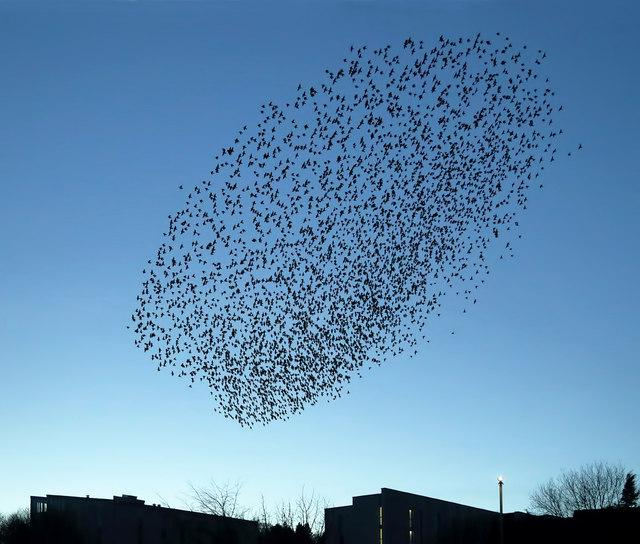
\includegraphics{media/ch1/image1.jpg}

}

\caption{\label{fig-ch1-img1}A flock of birds.}

\end{figure}%

Similar examples can be found in all natural sciences. Tornadoes, for
example, are made up of air molecules that also interact locally.
Tornadoes are unpredictable, self-organizing, global weather phenomena.
A famous chemical example is the Belousov---Zhabotinsky reaction, a
chemical oscillator (Kuramoto 1984). This reaction involves a mixture of
chemicals. As the reaction proceeds, the solution exhibits strikingly
colorful oscillations between clear and opaque or between different
colors, depending on the specific reactants used. We will see many more
examples in later chapters.

The prime example from psychology is the brain. About a hundred billion
neurons interact with thousands of other neurons in their neighborhood.
Compared to computers, brains are extremely energy-efficient, but like
all open systems, they do consume energy (the equivalent of a light bulb
according to Attwell and Iadecola 2002).
{\marginnote{\begin{footnotesize}Fast local interactions somehow form
global waves of electrical activity that make up thought processes and
even consciousness.\end{footnotesize}}} The letters you are reading
activate retinal neurons that initiate a cascade of electrical waves
across billions of neurons that somehow create your understanding of
this text (Roberts et al. 2019; Schöner 2020). How is this possible? For
me, this is the most fascinating scientific question of all time. It's
the main reason why I'm a psychologist and not a physicist. I view the
brain as the ultimate complex system.

\section{Emergentism}\label{sec-Emergentism}

What is the relation between complexity and reductionism? According to
reductionism, complex phenomena can be explained by reducing them to the
interactions of their individual parts or components. This raises two
questions, one related to weak emergence and one related to strong
emergence.

The first question is, why it is possible to do science in any field
other than physics, since ultimately chemistry, biology, and even
psychology are all about interacting elementary particles? Should we not
first finish the study of physics before starting to think about complex
molecules, cells, neurons, or higher-order human cognition?

Philip Anderson's renowned paper ``More Is Different'' convincingly
argues that the answer to this question is a resounding \emph{no} (P. W.
Anderson 1972). {\marginnote{\begin{footnotesize}Science is possible at
many different levels of description without fully understanding the
lower levels.\end{footnotesize}}} There is much to be said for
reductionism, but somehow the laws of quantum mechanics are irrelevant
when studying interactions between neurons or people. I don't think that
emergence in complex systems is inconsistent with a reductionist view of
science (Bechtel and Abrahamsen 2005). One could say that
complex-systems theory explains why emergent phenomena such as atoms or
neurons can be used as lower-order entities at even higher levels of
description to explain new higher-order phenomena, without being a
dualist.

This fundamental principle of emergence is what allows disciplines like
psychology to exist as distinct and independent fields of science (Fodor
1974). {\marginnote{\begin{footnotesize}``In the face of complexity, an
in-principle reductionist may be at the same time a pragmatic holist''
(Simon 1962).\end{footnotesize}}} The concept of level is central to
Herbert Simon's architecture of complexity, in which each subsystem is
itself a complex structure made up of smaller parts, and this pattern is
repeated at multiple levels.\footnote{See figure~\ref{fig-ch6-extra} for
  a visual illustration of this idea.} According to Simon, these nested
structures are ubiquitous in the natural world and in human-made systems
because they are robust and adaptable. For an in-depth discussion of
this level concept I refer to Wimsatt (1994).

The second, more controversial, question is whether emergent phenomena
have an independent causal role (strong emergence) or mainly have
descriptive value (weak emergence). Strong emergence is often associated
with downward causation (Chalmers 2006; Flack 2017; Kim 2006).
{\marginnote{\begin{footnotesize}Downward or circular causation is the
idea that higher-level entities or properties can influence the behavior
of lower-level entities or properties.\end{footnotesize}}}

I like to link this to the flocking example. Flocks of birds are
emergent phenomena that do not determine the behavior of the individual
birds. The birds only follow the local rules. Flocking is an example of
weak emergence. However, when predators enter the scene, things change.
Predators get confused by flocks of prey, not by the behavior of
individual birds. So the flock has some causal power. Moreover, the
birds react to the predator's movements. This could be seen as an
example of downward causation and thus strong emergence
(figure~\ref{fig-ch1-img4}). Recent work attempts to quantify such
causal emergence effects (see, e.g., Hoel, Albantakis, and Tononi 2013).

\begin{figure}

\centering{

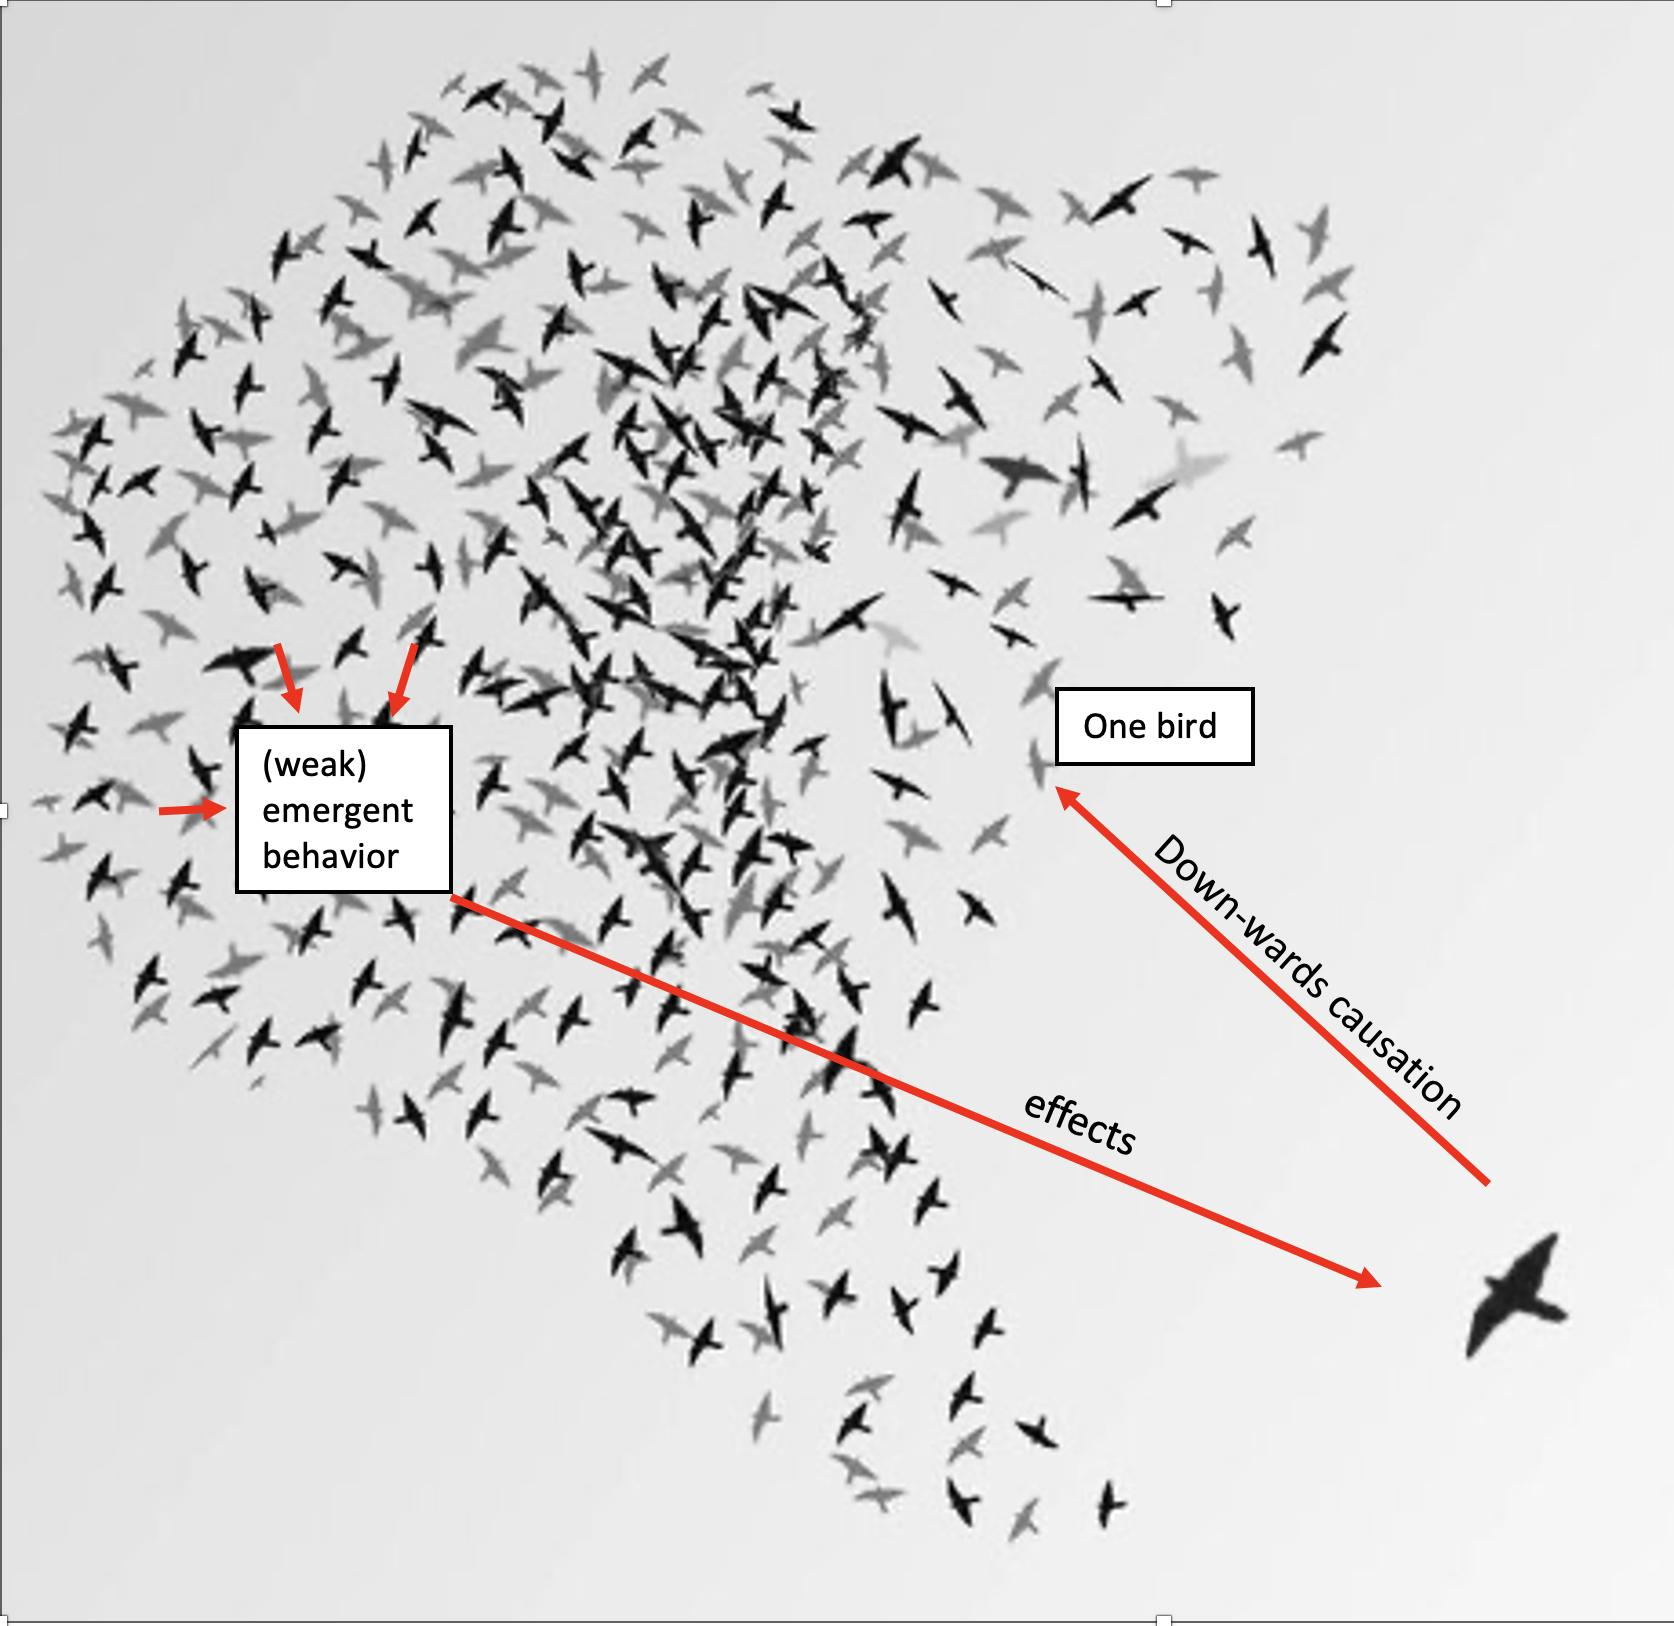
\includegraphics{media/ch1/image4.jpg}

}

\caption{\label{fig-ch1-img4}An illustration of downward or circular
causation in flocks due to a predator responding to the emerging
patterns of the flock and subsequently influencing the flight of
individual birds. (Adapted from \url{https://arxiv.org/abs/1108.1682})}

\end{figure}%

{\marginnote{\begin{footnotesize}Both weak and strong emergence are
essential to understanding psychological phenomena.\end{footnotesize}}}
Our minds, encompassing conscious thought, self-awareness, reasoning
abilities, natural language comprehension, emotions, and attitudes, are
not mere artifacts and cannot be simply reduced to intricate patterns of
neural activity. In my view, these mental constructs, such as
consciousness, possess their own causal influence, and this is one of
the reasons that psychology stands as a scientific discipline in its own
right.

Of course, the relationship between the mind and the brain is one of the
most debated topics in psychology. The neuro-reductionist view is
popular in the field of psychology, when it concerns the explanation of
both higher cognition (Schwartz et al. 2016) and psychological disorders
(for a critical review, see Borsboom, Cramer, and Kalis 2019).

\section{The field of psychology}\label{sec-The-field-of-psychology}

The study of complex systems in the natural sciences is highly
technical. I like to think of the field of complex systems as a toolbox
of empirical paradigms and mathematical models and techniques (Grauwin
et al. 2012). Models are often formulated in the form of difference or
differential equations and subjected to, for example, bifurcation
analysis. These are mathematical ways of describing the behavior of
complex systems. Additionally, advanced numerical analysis, commonly in
the form of computer simulation, is a standard approach. However,
educational programs in psychology do not usually include courses in
algebra, calculus and programming. Many psychologists lack the basic
knowledge and skills to apply the toolbox of complex-systems theory, as
these are not ordinarily part of the psychology curriculum.
Complex-systems research simply seems too complex for psychologists and
social scientists. One goal of this book is to provide psychologists
with a first introduction to this technical toolbox.

Unfortunately, there are additional complications in applying these
tools to our field. First, our subjects are much more complex than
flocks of birds or tornadoes and they display astonishing behavior. They
can do science! They can also walk out of the lab because they find the
experiment boring. This does not happen with lasers. Second, we have to
deal with the ethical constraints of experimenting on our subjects. We
cannot take them apart, a very successful approach in the natural
sciences. Finally, there is the measurement issue (Lumsden 1976; Michell
1999).

We tend to forget how incredibly precise the natural sciences,
especially physics, are. In 1985, Richard Feynman famously claimed that
the accuracy of calculating the size of the magnetic moment of the
electron was equivalent to measuring the distance from Los Angeles to
New York, a distance of over 3,000 miles, to the width of a human hair.
I find that shocking. Less famously, I would argue that psychologists
have not yet ``discovered'' continents and have no idea where New York
is. Our instruments generally fail to meet elementary requirements of
reliability and validity, we are plagued by replication failures, and
our theories are often imprecise (Eronen and Bringmann 2021).
{\marginnote{\begin{footnotesize}Navigating the behavioral and social
sciences and knowing which data to trust and which empirical phenomena
to model is an art in itself.\end{footnotesize}}}

This is all unfortunate because not only our brains but every subject in
our field seem to have the characteristics of a complex system. Social
systems are complex systems made up of individuals interacting to
produce emergent phenomena such as cultures and economic systems. The
human brain, the most complex system we know, is embedded in different
hierarchies of very complex social systems such as families, education,
economies, and cultures. We need the toolbox!

Despite all these problems, I'm not pessimistic. I believe that tangible
progress in the behavioral and social sciences is possible. It is not
that these sciences are completely unsuccessful. We know a lot about
people's attitudes, addictive behavior, cognition, and the social
systems in which they interact. We study these, with some success, using
advanced experimental designs, and we have developed (mainly) verbal
theories about almost everything.

We also have no choice; we must make progress. Personally, I feel a
strong tension between our struggle to elevate the behavioral and social
sciences as a science, on the one hand, and the enormous expectations of
society to deliver, on the other. Our most pressing global
problems---climate change, overpopulation, war and violence, poverty,
inequality, infectious diseases, addiction, to name but a few---are
unsolvable without breakthroughs in the behavioral and social sciences.
{\marginnote{\begin{footnotesize}J. Doyne Farmer: ``We have an
increasing need to model ourselves'' (Thurner 2016).\end{footnotesize}}}

The realization that the human mind in its social context is an
amazingly complex system also offers opportunities. Despite their
obvious differences, complex systems show remarkable similarities. A
predecessor of complex-systems theory, general-systems theory
(Bertalanffy 1969), explicitly assumed that all systems share important
characteristics. {\marginnote{\begin{footnotesize}Certain mechanisms and
phenomena seem to operate and to occur in similar ways at all possible
levels of description (Simon 1962).\end{footnotesize}}}. This is the
primary reason for providing numerous modeling examples in this book
that originate from disciplines beyond psychology.

An inspiring example for me comes from the study of shallow lakes
(Scheffer 2004). Shallow lakes tend to be either in a ``healthy'' state,
with clear water and a diverse population of fish and plants, or in an
``unhealthy'' turbid state. I like to compare these complex lake systems
in the turbid state to a person suffering from depression. This turbid
state usually occurs suddenly. There is a critical phosphorus load at
which the system turns over from being healthy to complete dominance by
algae and bream. Typical of this type of transition is the hysteresis
effect (figure~\ref{fig-ch1-img2}). This means that the turning point
from clear to turbid and from turbid to clear does not occur at the same
phosphorus load. The turning point to clear water only occurs at much
lower phosphorus loads. These tipping points may be so far apart that
reducing the cause, the phosphorus load, is not a viable option. Of
course, all sorts of interventions have been studied, such as
supplemental oxygen, chemicals, sunscreens, and stocking predatory fish.
These interventions have not been very successful, or only successful in
specific cases. The fact that they had some level of success brings to
mind the partial effectiveness of clinical interventions, such as those
used in the treatment of major depressive disorder.

\begin{figure}

\centering{

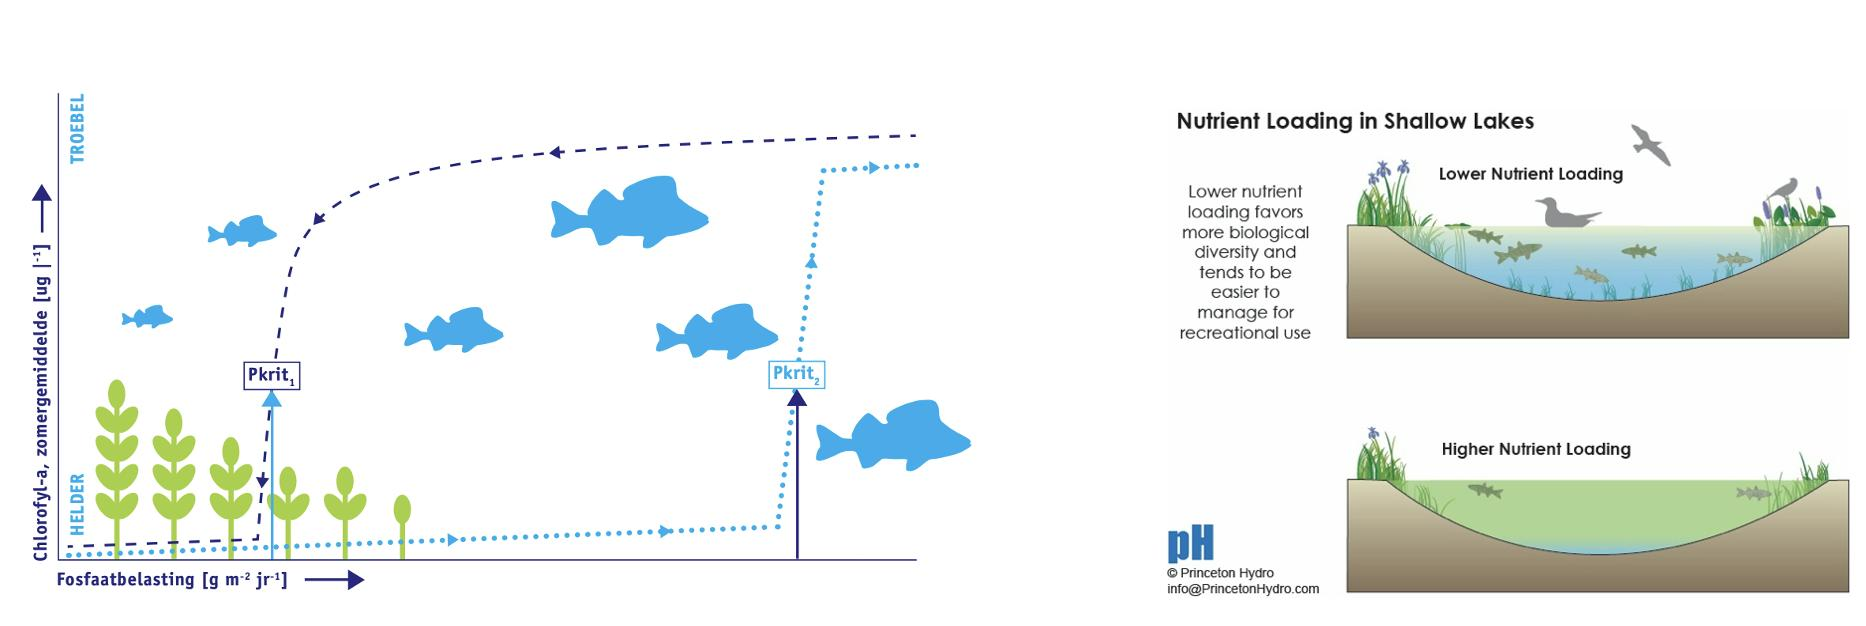
\includegraphics{media/ch1/image2.jpg}

}

\caption{\label{fig-ch1-img2}The transitions between clear and turbid
states of shallow lakes do not occur at the same phosphorus load. This
delay in jumps is called hysteresis. Hysteresis explains why transitions
are often difficult to reverse. This concept is discussed in detail in
Chapter~\ref{sec-ch3}.}

\end{figure}%

A breakthrough occurred in the 1980s. Removing all the fish proved to be
a very effective intervention. The ecologists caught almost all the fish
with nets during the winter. In the spring, a new, healthy equilibrium
emerged, characterized by aquatic plants, other fish species, and clear
water. This new state is often stable for long periods of time.
Remarkably, the analysis of the cause, the phosphorus load, was not part
of the solution: although the increasing phosphorus load is the primary
cause of the transition toward a turbid state, decreasing the phosphorus
load does not cause the system to transition back into the clear state.
{\marginnote{\begin{footnotesize}The dogma of intervention, that the
cause of the problem is the key to the solution, does not necessarily
apply to complex systems.\end{footnotesize}}} What this means for our
thinking about depressive disorders will be discussed in Chapters
\ref{sec-ch5n} and \ref{sec-ch6}.

I will discuss three reasons to be somewhat optimistic, based on three
key observations about complex systems. The first key observation has to
do with simplification, the second with the tendency of complex systems
to be characterized by a limited number of stable states, and the third
is that all complex systems seem to be describable as some kind of
network. Simplification is perhaps the most important one.

\section{The art of simplification}\label{sec-The-art-of-simplification}

{\marginnote{\begin{footnotesize}Einstein supposedly said that
everything should be made as simple as possible, but not one bit
simpler.\end{footnotesize}}} A fascinating and instructive example is
the traffic jam, which is made up of many people, with their amazingly
complex brains, in modern cars full of advanced technology. Where to
start modeling such a complex phenomenon? The answer is astonishing. It
seems that we can reduce people in cars to simple blocks in a lane,
speeding up when there is space in front of the artificial car and
braking when they get too close to the car in front. All lower levels of
modeling are ignored. This is even simpler than a flock of birds.

It is not difficult to set up a computer simulation for this case. I
recommend that you spend some time playing around with an
example.\footnote{A nice example is
  \url{https://www.traffic-simulation.de/})} It does not take long to
see that traffic jams can easily form and have an unexpected property:
while cars move forward, traffic jams move backward! Another interesting
observation is that variance in speed causes congestion. But the
variance is not in any of the cars. Variance and congestion are
properties at a higher level of description. With this simulation, you
can study different types of traffic situations and interventions. This
type of simulation seems to be very useful for designing of motorways
(Barceló 2010; Treiber, Hennecke, and Helbing 2000). There are actually
different ways to model traffic jams. Jusup et al. (2022) distinguish
between fluid-dynamical, kinetic, car-following, coupled-map lattice,
and cellular automata models. They all reproduce many phenomena of real
traffic jams.

{\marginnote{\begin{footnotesize}In complex systems, the qualitative
properties of large-scale phenomena do not depend on microscopic
details.\end{footnotesize}}} Only higher-level properties are relevant
to global behavior. A large part of the art of science is finding of the
right level of simplification. Suppose we are studying smoking. Do we
model the effects of nicotine on blood vessels, how the hand with the
cigarette moves from the mouth to the ashtray, or the number of
cigarettes smoked per day? Do we include the effects of marketing and
the smoker's social network?

What is relevant and what can be ignored? It can be challenging to
provide a definitive answer for specific cases. Nevertheless, in
general, it can be said that there is a limit to the lower levels that
must be considered. When examining traffic jams, it is necessary to
incorporate certain characteristics of individuals and vehicles, but
delving deeper into topics like neuronal firing, DNA replication, or the
intricate workings of car batteries becomes irrelevant. At that level of
modeling, there is no relevant information that would alter the
explanation of a traffic jam.

The traffic example shows that extreme simplification is sometimes
possible and necessary. But finding the right level of simplification is
not a simple task at all. In Borsboom et al. (2021) we propose a
\emph{theory-construction methodology} (TCM) consisting of five steps:

\begin{enumerate}
\def\labelenumi{\arabic{enumi}.}
\tightlist
\item
  Identify the empirical phenomena that become the target of
  explanation.
\item
  Formulate a set of theoretical principles that putatively explain
  these phenomena.
\item
  Use this set or prototheory to construct a formal model, a set of
  model equations that encode the explanatory principles.
\item
  Analyze the explanatory adequacy of the model, i.e., whether it
  actually reproduces the phenomena identified in step 1.
\item
  Determine whether the explanatory principles are sufficiently
  parsimonious and substantively plausible.
\end{enumerate}

The article explains these steps in detail and provides an example, the
mutualism model of general intelligence, which is explained in
Chapter~\ref{sec-ch6} of this book.

I will add a few comments to this list of steps. First of all, step 1 is
key. It is crucial to be precise about defining the phenomena to be
explained. Phenomena are not the same as data. Data are particular
empirical patterns (a concrete dataset), whereas phenomena are general
empirical patterns, stable and general features of the world (Haig
2014). As noted above, in the behavioral and social sciences, it is not
always clear which data patterns can be trusted. In the last ten years,
the replication crisis has led to a revolution in psychological methods,
but many results are collected using potentially biased methods. One
problem is publication bias: negative results are still harder to
publish than results that support hypotheses. In other cases, the
results of different studies contradict each other, and meta-analyses
show weak effects at best. {\marginnote{\begin{footnotesize}Drawing up a
list of the most important phenomena on a topic, such as depression,
forgetting, or discrimination, is often a challenge.\end{footnotesize}}}

The second observation is that taking these steps is not a linear
process. Often, when developing a model, you realize that some important
information is missing from the list of phenomena. For example, you
might be modeling addiction, but suddenly you need information about the
combination of addictive substances that people use. And such simple
questions are often impossible to answer. You can spend days searching
the literature for information that you expect to be readily available,
only to find that many basic things are simply unknown.

A third observation is that formal modeling is mostly a matter of
analogical reasoning. You have to study many examples of complex-systems
models to understand how to construct such a model. Indeed, in my own
work I often use established models developed in physics and biology as
a base model. We will see many examples of this later.

Fourth, good models do not build in phenomena but explain them from
basic principles. By building in, I mean that a phenomenon should not be
an assumption of the model. An example would be a model that says that
variance in the speed of cars causes traffic jams. Such a model may
explain other things, but not the role of speed variance, because that
effect is part of the assumptions. Models that make such assumptions are
called phenomenological models. We will see examples of phenomenological
models of complex systems, as well as explanatory models, where the
latter are based on fundamental principles.
{\marginnote{\begin{footnotesize}Building real explanatory models in our
fields is extremely difficult.\end{footnotesize}}}

Fifth, it is my conviction that a metaphorical use of the
complex-systems approach should be avoided by using concrete formal
models (Dongen et al. 2024). It is crucial to strive for the highest
level of scientific rigor. There are no special, more lenient,
methodological rules for complex-systems research (van der Maas 1995).

\section{A limited number of
equilibria}\label{sec-A-limited-number-of-equilibria}

The first key observation was that complex systems can be simplified.
The second is that complex systems tend to be characterized by a limited
number of equilibria. An important example is water. Water normally
exists in either a solid, liquid, or gaseous state (leaving aside the
plasma state). These are stable states over wide ranges of temperature
and pressure.

A biological example is the life stages of a butterfly (egg,
caterpillar, chrysalis, and butterfly). Except for brief periods of
transition, these insects are in one of these four relatively stable
states. Another example is the horse, which is either standing still,
walking, trotting, or galloping. I am convinced that we must always
start by identifying the equilibria of a complex system. This also
applies to psychological and social science applications. A bipolar
disorder seems to be characterized by two stable states (depressive and
manic). In the case of addiction, we may think of a three states:
non-use, recreational use, and heavy use (Epskamp et al. 2022).
Similarly, we could identify the stages in falling in love, in
understanding of calculus, in sleeping, and in radicalization.

Identifying discrete stages turns out to be more difficult than it first
appears. {\marginnote{\begin{footnotesize}There is an ongoing discussion
about the number of stages, even for something like sleep (Boostani,
Karimzadeh, and Nami 2017; de Mooij et al. 2020).\end{footnotesize}}} It
is often possible to come up with more substages. For instance, in the
case of horse movement, people tend to further subdivide trot into three
forms (working, medium, and collected). Subdivisions are also made in
the case of heavy alcohol consumption (Leggio et al. 2009). It is
possible to use objective statistical methods to support such
classifications using modern machine-learning techniques (automatic
clustering) as well as more traditional means (finite mixture models,
latent class analysis). I will say more about this in
section~\ref{sec-Multimodality}.

A further complication is that equilibria come in different forms. The
simplest form consists of fixed points or point attractors, an example
being a ball lying in a valley. Under undisturbed conditions, the ball
could also be resting on top of a hill, which is an unstable
equilibrium. An equilibrium could also be a limit cycle or oscillator.
For example, two pendulums could swing in phase or out of phase. It gets
even weirder when we consider strange attractors, which often take the
form of fractals. This will be explained in more detail in the next two
chapters.

Finally, it has also been argued that many complex systems, especially
living systems, never reach equilibrium because they are constantly
perturbed (Groot and Mazur 2013). {\marginnote{\begin{footnotesize}I see
this distinction between equilibrium and non-equilibrium complex systems
as gradual.\end{footnotesize}}} Some complex psychological systems are
clearly stable over the long term. Unfortunately, this is true of many
psychological disorders. In contrast, my understanding of the world,
psychological science, and complex-systems research is better described
as a continuously perturbed non-equilibrium system with just enough
stability to write this book (once).

I would claim that many psychological complex systems tend to be in one
attractor state most of the time, but they occasionally change states.
If certain control parameters slowly change their values, the current
equilibrium can become unstable and a transition to another equilibrium
can occur. This is what happens when we lower the temperature of water
to below zero. {\marginnote{\begin{footnotesize}Transitions can occur in
many ways, also depending on the types of equilibria
involved.\end{footnotesize}}} The family of transition models is
described by bifurcation theory. This is explained in
Chapter~\ref{sec-ch3}, where we focus on a very important transition
model, the cusp catastrophe, and in Chapter~\ref{sec-ch4n}, which
considers dynamical systems models.

\section{Networks are everywhere}\label{sec-Networks-are-everywhere}

The third key observation of great relevance to the attempt to use
complex-systems modeling in psychology is that complex systems are
networks, as they consist of interacting subelements. For me, the
network is the most interdisciplinary research topic in modern science.
Magnets, ecosystems, the brain, the internet, and social networks are
prime examples. {\marginnote{\begin{footnotesize}Network science is a
huge area of research with many fundamental insights and an important
tool in modern psychological science.\end{footnotesize}}}

Two applications in psychology are well known: the first is the study of
neural networks, which started seventy years ago and has become the main
foundation of the artificial intelligence (AI) revolution of the last
ten years. In Chapter~\ref{sec-ch5n} I will discuss neural networks. The
second is social networks, the simplest example being dyadic
interactions. Social media such as Facebook are infamous examples. Key
ideas relate to concepts such as weak and strong ties, central hubs and
homophily, which are discussed in Chapters 6 and 7. The analysis of
social-network data is an exciting area of research (Scott 2011). It
focuses on understanding how social entities are connected and how these
connections influence various outcomes and behaviors. Connections
between nodes (e.g., individuals, organizations, communities) can be
based on different dimensions, such as friendship, communication,
collaboration, information flow, or any other form of social
interaction. These interactions may also change over time, which is
studied in social-network dynamics (Snijders 2001).\footnote{Statnet.org
  provides an overview of R packages for social network analysis.}

Chapter~\ref{sec-ch6} focuses on a novel use of networks, which I call
\emph{network psychology}. This is a level of description between neural
networks and social networks. It involves modeling intelligence,
attitudes, and psychological disorders at the individual level.
Intelligence, for example, is modeled as an ecosystem of cooperating
cognitive functions. This is radically different from the standard view
that general intelligence is due to \(g\), a single underlying source.
In the mutualism model of general intelligence (van der Maas et al.
2006), the observed positive correlations between scores on subtests of
IQ test batteries are due to cumulative reciprocal developmental
interactions between cognitive subsystems such as working memory,
spatial cognition, and language.

{\marginnote{\begin{footnotesize}Similarly, depression can be thought of
as a network of mutually reinforcing symptoms.\end{footnotesize}}} As
another example, sleep problems, a symptom of depression, can lead to
increased fatigue and difficulty concentrating, which in turn can affect
a person's ability to manage daily tasks and engage in social
activities. This can then lead back to poorer sleep quality, creating a
cyclical pattern in which each symptom reinforces the others. This new
view of mental disorders originated in our research group and is now
very popular (Robinaugh et al. 2020). One reason for this is that many
statistical techniques have been developed to investigate this network
approach.

The latest line of this research is the integrated study of
psychological and social networks (van der Maas, Dalege, and Waldorp
2020). Chapter~\ref{sec-ch7} deals with models in which psychological
network models of attitudes are nested within social networks of opinion
change. This model provides a new explanation of polarization.
{\marginnote{\begin{footnotesize}In the process of polarization,
nonlinear intrapersonal and interpersonal dynamics
interact.\end{footnotesize}}}

\section{Methods for investigating complex
systems}\label{sec-Methods-for-Investigating-complex-systems}

Complex systems are studied in various ways across different
disciplines. We use computer simulations to examine the emergence in
complex system models, analyze their unpredictable behavior, categorize
the types of tipping points involved, derive equations that describe the
overall behavior of complex systems, collect and analyze time-series
data, or experimentally disrupt the system to test its resilience.
Following Sayama (2015), I categorize the models and methods into two
groups: those for systems with a small number of variables and those for
systems with many variables.

The first category is referred to as \emph{nonlinear dynamical system
theory}, which encompasses chaos theory and catastrophe or bifurcation
theory. The second category includes tools for studying multi-element
systems, such as agent-based modeling and network theory. One might
assume that the first category is irrelevant to complex systems, which
by definition have many variables. However, it has been found that the
global behavior of complex systems can often be described with a small
number of variables, often just one, that behave in a highly nonlinear
manner.{\marginnote{\begin{footnotesize}I consider nonlinear dynamical
system theory an essential part of complex-systems
research.\end{footnotesize}}}

This categorization is reflected in the book's structure. The next three
chapters are devoted to systems with a small number of variables:
Chapter~\ref{sec-ch2} discusses chaos theory, Chapter~\ref{sec-ch3}
addresses sudden transitions as studied in catastrophe and bifurcation
theory, and Chapter~\ref{sec-ch4n} provides an introduction to modeling
dynamical systems.

In the second part of the book, we shift our focus to tools for studying
systems with many variables, particularly agent-based modeling of
self-organization in Chapter~\ref{sec-ch5n}, network modeling in
Chapter~\ref{sec-ch6}, and the application of both to psychosocial
systems in Chapter~\ref{sec-ch7}.

\section{Other work and sources}\label{sec-Other-work-and-sources}

The complex-systems approach has often been introduced as the next new
thing, but those days are gone. Even in psychology it can no longer be
considered a new approach. Many different research groups have used the
toolbox of complex-systems research in all areas of psychology. This
book will give many examples. One could even argue that a lot of work
has been done that could be considered complex-systems research but has
not been published under that heading. For example, most neural-network
models of psychological processes are complex-systems models because
they investigate emergent computational properties of the interaction of
neural units. This is also true of much work in mathematical psychology,
for example when differential equations are used to study dynamical
systems. Older work in complex-systems research has often been published
with reference to nonlinear dynamical systems. Other related approaches
are computational social science and agent-based modeling.

Today, there are many interdisciplinary centers or hubs for complexity
research. The Santa Fe Institute in Santa Fe, New Mexico, is the pioneer
of complexity science. Its summer schools are highly recommended. Other
examples are the Complexity Science Hub in Vienna, Austria, and the
Centre for Complexity Science at the University of Warwick, in England.
In my own country, the Netherlands, we have at least four of these
centers. I'm a principal investigator at the Institute for Advanced
Study in Amsterdam and an external faculty member at the Santa Fe
Institute.

It is impossible to give a balanced review of all past and ongoing work
on complex systems. I'm naturally somewhat biased toward our own work
and contributions, but I do my best to point out relevant work. As a
general resource to complex systems research with a bit less technical
approach, I recommend the book of Mitchell (2009); for a bit more
mathematical approach I recommend the books of Serra and Zanarini
(1990), Sayama (2015), and Thurner, Klimek, and Hanel (2018). Overviews
of work in psychology are provided by Guastello, Koopmans, and Pincus
(2008) and Port and Gelder (1995). Other great books are written by
Heath (2000) and Kelso (1995).

\section{Exercises}\label{sec-Exercises-ch1}

\begin{enumerate}
\def\labelenumi{\arabic{enumi})}
\item
  Visit \url{https://www.traffic-simulation.de/}. In what direction do
  traffic jams move? For roundabouts: What is a bad priority rule? Do
  traffic jams appear and disappear for the same values of critical
  parameters? Take for instance the ring road and vary Politeness. (*)
\item
  Give your own example of a psychological process or theory where
  different stable stages or states are distinguished. (*)
\item
  Could consciousness be seen as a process of downward causation?
  Explain your answer. (**)
\end{enumerate}

\bookmarksetup{startatroot}

\chapter{Chaos and unpredictability}\label{sec-ch2}

\section{Introduction}\label{sec-Introduction-ch2}

Suppose we have immense amounts of genetic, biological, and
psychological data on millions of participants and knowledge of all
relevant environmental factors. Suppose also that these huge amounts of
data are of fantastic quality. Using state-of-the-art machine-learning
models and powerful computing resources, we could build advanced
statistical models that include main and higher-order interaction
effects of all variables, even incorporating nonlinear transformations.
Even then, prediction may not be possible. Why? Because of a phenomenon
called \emph{deterministic chaos}.
{\marginnote{\begin{footnotesize}Deterministic chaos refers to the
behavior of complex systems that is highly sensitive to initial
conditions, leading to unpredictable and seemingly random results
despite being governed by deterministic laws.\end{footnotesize}}}

Chaos is one of the most spectacular phenomena in complex systems, and
as psychologists we should know the basic results of chaos theory. It is
also great fun to learn about chaos and it allows me to introduce many
key concepts that we need in later chapters.

In my opinion, the direct applicability of chaos theory to psychology
and social science is somewhat limited. For a long time, researchers
have tried to show chaos in time series of psychophysiological measures,
but this seems to be difficult. I will briefly review this work at the
end of the chapter. The relevance of chaos theory may lie not in its
application but in its fundamental implication for prediction. What
chaos theory basically shows is that even in the best of circumstances,
where we have very accurate models and data, long-term prediction might
be impossible. {\marginnote{\begin{footnotesize}This is known as the
butterfly effect (E. N. Lorenz 1963): a butterfly flaps its wings in
India, and that tiny change in air pressure could eventually cause a
tornado in Iowa. How this works will become clear in this
chapter.\end{footnotesize}}}

\section{The population growth of
rabbits}\label{sec-The-population-growth-of-rabbits}

Chaos theory consists of many deep mathematical results, but
understanding the basics of chaos is not so hard. Below I will explain
chaos in difference equations at a very basic level of mathematics and
programming. The elementary example is the famous logistic map, usually
introduced as a model of population growth, for instance, of rabbits.
Suppose we have rabbits on an island, and they start to multiply. What
would the mathematical model be for such a process?

{\marginnote{\begin{footnotesize}Population growth is a typical example
of a dynamical system, as it is a model of change.\end{footnotesize}}}
In general, in a dynamical system, the change or growth of a variable
(say \(X\)) depends on the current state and some parameters. Time plays
a very special role. We can use discrete or continuous time steps. In
the first case, which is the focus of this chapter, we use difference
equations; in the second case, we use differential equations. In the
logistic map, time is discrete (population growth takes place in
generations). The simplest dynamical model for the population growth of
rabbits is:

\begin{equation}\phantomsection\label{eq-ch2-1}{
X_{t + 1} = rX_{t}}\end{equation}

This says that the new value of \(X\) is determined by the previous
value of \(X\), multiplied by \(r\). In this equation \(r\) is the
growth rate. We can simulate this model by choosing a value for \(r\),
\(r=2\), for instance. We also need an initial value, say \(X_{0} = 1.\)
If this is completely new to you, enter some values repeatedly. You will
see exponential growth
(\(X_{1} = 2,\ X_{2} = 4,X_{3} = 8,X_{4} = 16,\ etc.)\). In R we can
simulate this using a for loop (the result is shown in
figure~\ref{fig-ch2-img1}).

\begin{Shaded}
\begin{Highlighting}[]
\NormalTok{n }\OtherTok{\textless{}{-}} \DecValTok{15}
\NormalTok{r }\OtherTok{\textless{}{-}} \DecValTok{2}
\NormalTok{x }\OtherTok{\textless{}{-}} \FunctionTok{rep}\NormalTok{(}\DecValTok{0}\NormalTok{,n)}
\NormalTok{x[}\DecValTok{1}\NormalTok{] }\OtherTok{\textless{}{-}} \DecValTok{2} \CommentTok{\# initial state X0 = 1 and thus X1 = 2}
\ControlFlowTok{for}\NormalTok{ (i }\ControlFlowTok{in} \DecValTok{1}\SpecialCharTok{:}\NormalTok{(n }\SpecialCharTok{{-}} \DecValTok{1}\NormalTok{))}
\NormalTok{  x[i }\SpecialCharTok{+} \DecValTok{1}\NormalTok{] }\OtherTok{\textless{}{-}}\NormalTok{ r }\SpecialCharTok{*}\NormalTok{ x[i]}
\FunctionTok{plot}\NormalTok{(x, }\AttributeTok{type =} \StringTok{\textquotesingle{}b\textquotesingle{}}\NormalTok{, }\AttributeTok{xlab =} \StringTok{\textquotesingle{}time\textquotesingle{}}\NormalTok{, }\AttributeTok{bty =} \StringTok{\textquotesingle{}n\textquotesingle{}}\NormalTok{)}
\end{Highlighting}
\end{Shaded}

\begin{figure}

\centering{

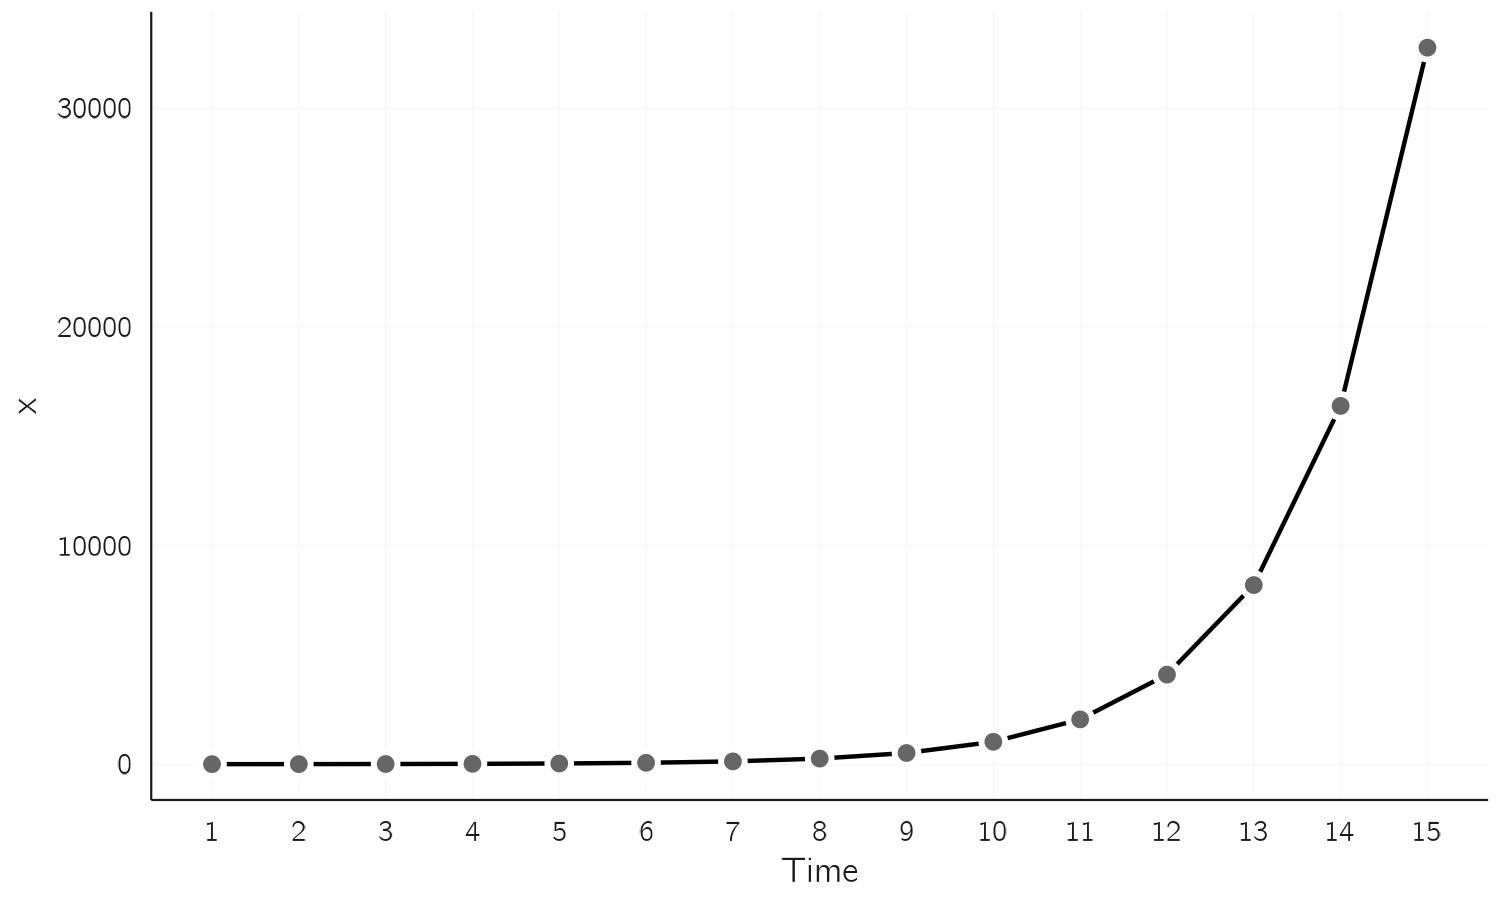
\includegraphics[width=8cm,height=\textheight]{media/ch2/fig-ch2-img1.jpg}

}

\caption{\label{fig-ch2-img1}Exponential growth.}

\end{figure}%

Note that we can find any \(X_{t}\) given \(X_{0}\) by iterating the
model as we do in the for loop. \(X_{t}\) is called the solution.
Simulation is a bit odd in this case. We can compute the solution
analytically. It is \(X_{t} = X_{0}r^{t}\). Thus for
\(X_{15} = 1 \times 2^{15} = 32768\).
{\marginnote{\begin{footnotesize}For more complex models, the analytical
solution is often not available, and we have to use simulation (the
numerical solution).\end{footnotesize}}}

Note that the exponential model ignores the fact that population growth
is limited by resources. At some point food will become scarce. One way
of making the model, introduced by Verhulst in 1838, more realistic is
to add a growth-limiting term:

\begin{equation}\phantomsection\label{eq-ch2-2}{
X_{t + 1} = f\left( X_{t} \right) = rX_{t}\left( 1 - \frac{X_{t}}{K} \right)}\end{equation}

What is the effect of this addition to the equation? If \(X\) is much
smaller than the resource \(K\), then the second term,
\(\left( 1 - {X_{t}}/{K} \right)\), is close to 1 and we will see
exponential growth. But as \(X\) approaches \(K\), this term becomes
very small, reducing the effect of exponential growth. \(X\) does not
actually grow up to \(K\), but to a lower value, if it converges at all.
We are going to see this in a moment. It also turns out that the actual
value of \(K\) is not of interest. Changing \(K\) does not change the
qualitative behavior. Therefore, \(K\) is usually set to 1, scaling the
population \(X\) between 0 and 1. The only remaining parameter is \(r\).
Changing \(r\), however, leads to a number of surprising
behaviors.\footnote{Verhulst proposed this model in the form of a
  differential equation in continuous time. We will discuss this type of
  model in Chapter~\ref{sec-ch4n}. In continuous time, nothing
  particularly spectacular happens, and we only see the kind of behavior
  displayed in figure~\ref{fig-ch2-img2}.}

\section{Stable and unstable fixed
points}\label{sec-Stable-and-unstable-fixed-points}

Let us study a ``boring'' case first, \(r = 2\)
(figure~\ref{fig-ch2-img2}).

\begin{Shaded}
\begin{Highlighting}[]
\NormalTok{n }\OtherTok{\textless{}{-}} \DecValTok{15}\NormalTok{; r }\OtherTok{\textless{}{-}} \DecValTok{2}\NormalTok{; x }\OtherTok{\textless{}{-}} \FunctionTok{rep}\NormalTok{(}\DecValTok{0}\NormalTok{,n)}
\NormalTok{x[}\DecValTok{1}\NormalTok{] }\OtherTok{\textless{}{-}}\NormalTok{ .}\DecValTok{01} \CommentTok{\# initial state}
\ControlFlowTok{for}\NormalTok{ (i }\ControlFlowTok{in} \DecValTok{1}\SpecialCharTok{:}\NormalTok{(n }\SpecialCharTok{{-}} \DecValTok{1}\NormalTok{))}
\NormalTok{  x[i }\SpecialCharTok{+} \DecValTok{1}\NormalTok{] }\OtherTok{=}\NormalTok{ r }\SpecialCharTok{*}\NormalTok{ x[i] }\SpecialCharTok{*}\NormalTok{ (}\DecValTok{1} \SpecialCharTok{{-}}\NormalTok{ x[i])}
\FunctionTok{plot}\NormalTok{(x, }\AttributeTok{type =} \StringTok{\textquotesingle{}b\textquotesingle{}}\NormalTok{, }\AttributeTok{xlab =} \StringTok{\textquotesingle{}time\textquotesingle{}}\NormalTok{, }\AttributeTok{bty =} \StringTok{\textquotesingle{}n\textquotesingle{}}\NormalTok{)}
\end{Highlighting}
\end{Shaded}

\begin{figure}

\centering{

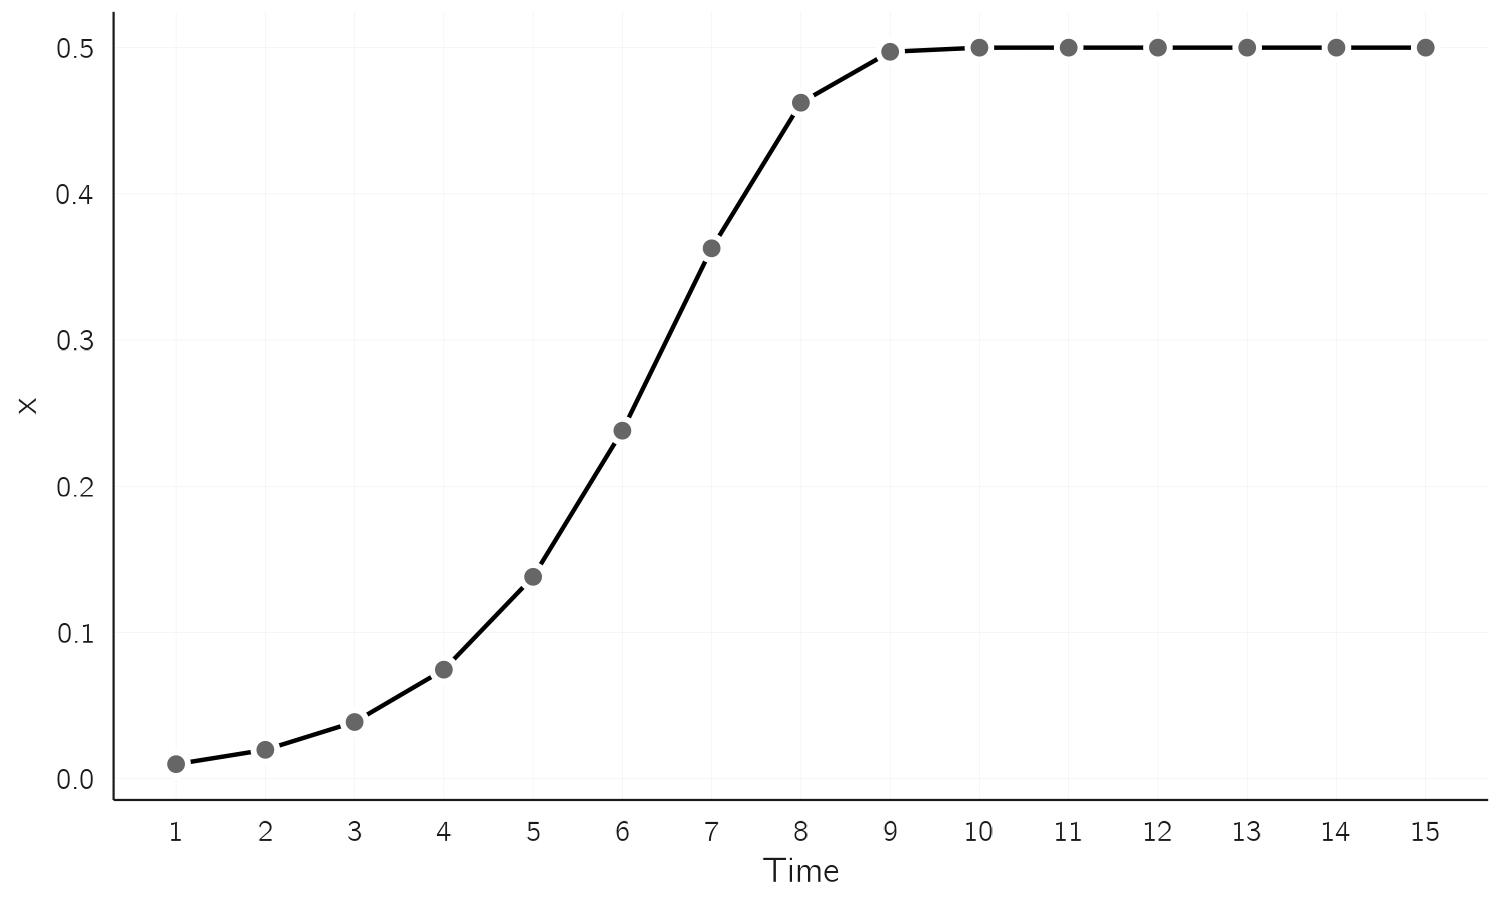
\includegraphics[width=8cm,height=\textheight]{media/ch2/fig-ch2-img2.jpg}

}

\caption{\label{fig-ch2-img2}The \(r=2\) case.}

\end{figure}%

This is the simple case. The population initially develops exponentially
but then levels off and reaches a stable state at \(X = .5\). We need to
understand a bit more about it. What you see here is that we have gone
from an unstable initial state to a stable state, a point attractor. The
next code shows that this point attractor attracts from a wide range of
initial values, but not all.

\begin{Shaded}
\begin{Highlighting}[]
\NormalTok{n }\OtherTok{\textless{}{-}} \DecValTok{30}\NormalTok{; r }\OtherTok{\textless{}{-}} \DecValTok{2}\NormalTok{; x }\OtherTok{\textless{}{-}} \FunctionTok{rep}\NormalTok{(}\DecValTok{0}\NormalTok{,n)}
\ControlFlowTok{for}\NormalTok{ (init }\ControlFlowTok{in} \FunctionTok{seq}\NormalTok{(}\DecValTok{0}\NormalTok{, .}\DecValTok{7}\NormalTok{, }\AttributeTok{by =}\NormalTok{ .}\DecValTok{01}\NormalTok{))}
  \CommentTok{\# start from different initial values}
\NormalTok{\{ }
\NormalTok{  x[}\DecValTok{1}\NormalTok{] }\OtherTok{\textless{}{-}}\NormalTok{ init}
  \ControlFlowTok{for}\NormalTok{ (i }\ControlFlowTok{in} \DecValTok{1}\SpecialCharTok{:}\NormalTok{(n }\SpecialCharTok{{-}} \DecValTok{1}\NormalTok{))}
\NormalTok{    x[i }\SpecialCharTok{+} \DecValTok{1}\NormalTok{] }\OtherTok{\textless{}{-}}\NormalTok{ r }\SpecialCharTok{*}\NormalTok{ x[i] }\SpecialCharTok{*}\NormalTok{ (}\DecValTok{1} \SpecialCharTok{{-}}\NormalTok{ x[i])}
  \ControlFlowTok{if}\NormalTok{ (x[i] }\SpecialCharTok{==} \DecValTok{0}\NormalTok{)}
    \FunctionTok{plot}\NormalTok{(x,}\AttributeTok{type =} \StringTok{\textquotesingle{}l\textquotesingle{}}\NormalTok{,}\AttributeTok{xlab =} \StringTok{\textquotesingle{}time\textquotesingle{}}\NormalTok{,}\AttributeTok{bty =} \StringTok{\textquotesingle{}n\textquotesingle{}}\NormalTok{,}\AttributeTok{ylim =} \FunctionTok{c}\NormalTok{(}\DecValTok{0}\NormalTok{, .}\DecValTok{8}\NormalTok{),}\AttributeTok{col =} \StringTok{\textquotesingle{}red\textquotesingle{}}\NormalTok{)}
  \ControlFlowTok{else}
    \FunctionTok{lines}\NormalTok{(x)}
\NormalTok{\}}
\end{Highlighting}
\end{Shaded}

If we start exactly at 0, \(X\) stays at 0 So, 0 is an equilibrium too,
but a special one. It is an unstable fixed point. A small perturbation
will cause \(X\) to move to .5, the stable fixed point. All initial
values in close proximity of 0 will move away from 0 (repellent), but if
\(X = 0\) exactly, then it remains 0 for all time. So, \(X = 0\) is a
fixed point but unstable (figure~\ref{fig-ch2-img1}).
{\marginnote{\begin{footnotesize}Fixed points can be stable or
unstable.\end{footnotesize}}}

\begin{figure}

\centering{

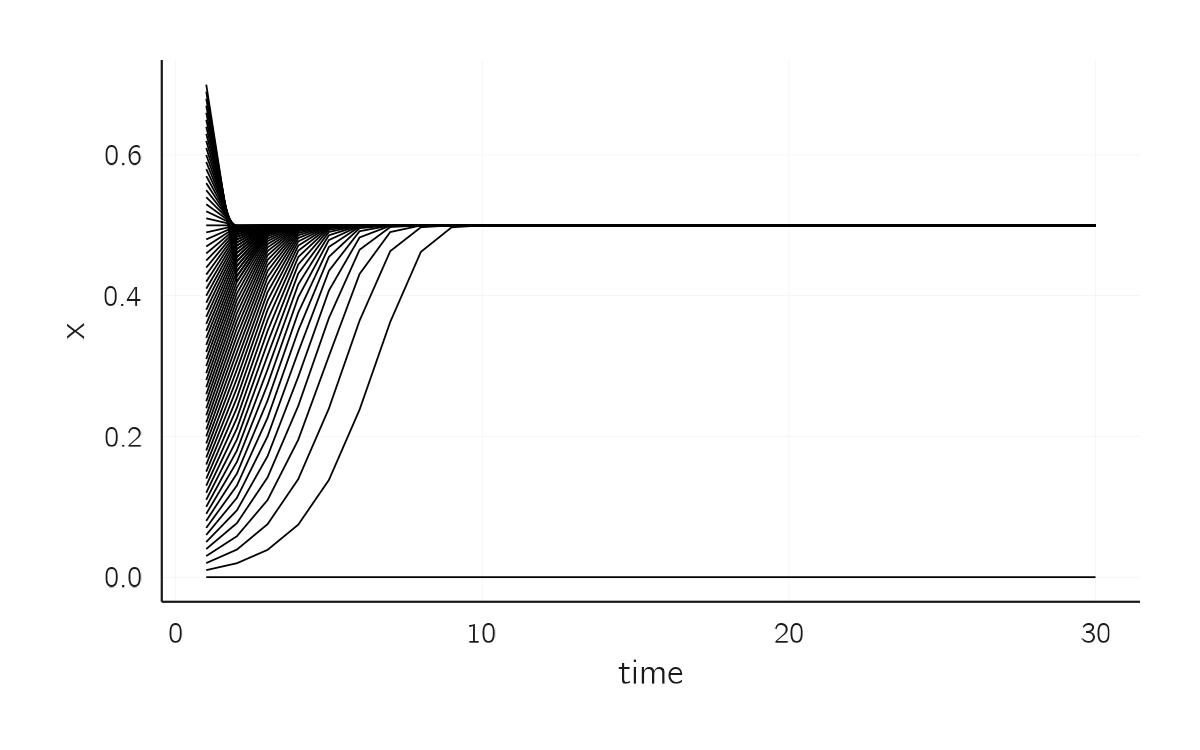
\includegraphics[width=10cm,height=\textheight]{media/ch2/fig-ch2-img3.jpg}

}

\caption{\label{fig-ch2-img3}Illustration of stable and unstable fixed
points. For many initial values, \(X = .5\) is an attractor. \(X = 0\)
is an unstable fixed point. Only if we start exactly at 0 do we stay
there.}

\end{figure}%

This concept of equilibrium, stable or unstable, is crucial for later
chapters. The essence of the next chapter is to change a control
parameter, here \(r\), and study how the pattern of equilibria (the
equilibrium landscape) changes. You can easily do this yourself by
setting \(r = .9\). For \(r < 1\), there is only stable attractor (0).

Simulating this is not really necessary. One has to realize that a fixed
point (\(X^{*}\)) is found when \(X_{t + 1} = X_{t} = X^{*}\). See for
yourself that:

\[
\begin{gathered}
X_{t + 1} = X_{t} = X^{*} \\
X^{*} = rX^{*}( 1 - X^{*}) \\
X^{*} = 0\ or\ 1 = r - rX^{*} \\
X^{*} = 0\ or\ X^{*} = \frac{r - 1}{r} \\
\end{gathered}
\]

So 0 and \((r - 1)/r\) are fixed points. Indeed, for \(r = 2\), we have
seen that 0 and .5 are equilibria, one stable and one unstable. To
determine whether fixed points are stable, we look at the derivative of
the function, \(f^{'}(x)\), which, as you can easily check, is
\(r - 2rX\).

The fixed point is stable if the absolute value of the derivative in the
fixed-point value is less than 1.\footnote{It is not too difficult to
  understand why this is. If you Google search ``fixed points of
  difference equations,'' you will quickly arrive at stackexchange.com,
  where several insightful explanations are given.} For \(r = 2\) the
fixed points are 0 and .5.
\(\left| f^{'}\left( X^{*} = 0 \right) \right| = |2 - 0| = 2\), which is
greater than 1 and thus \(X^{*} = 0\) is unstable.
\(\left| f^{'}\left( X^{*} = .5 \right) \right| = |2 - 2 \times 2 \times .5| = 0\),
which is less than 1 and thus \(X^{*} = .5\) is stable. You can check
for yourself that \(X^{*}=(r - 1)/r\) is stable for \(1 < r < 3\), both
with the R-code and with the absolute value of the derivative.

\section{Limit cycles}\label{sec-Limit-cycles}

So at \(r = 3\) the fixed point or \((r - 1)/r\) becomes unstable. Let's
study some cases. The plots in figure~\ref{fig-ch2-img4} are made with
the code for figure~\ref{fig-ch2-img2}.

\begin{figure}

\centering{

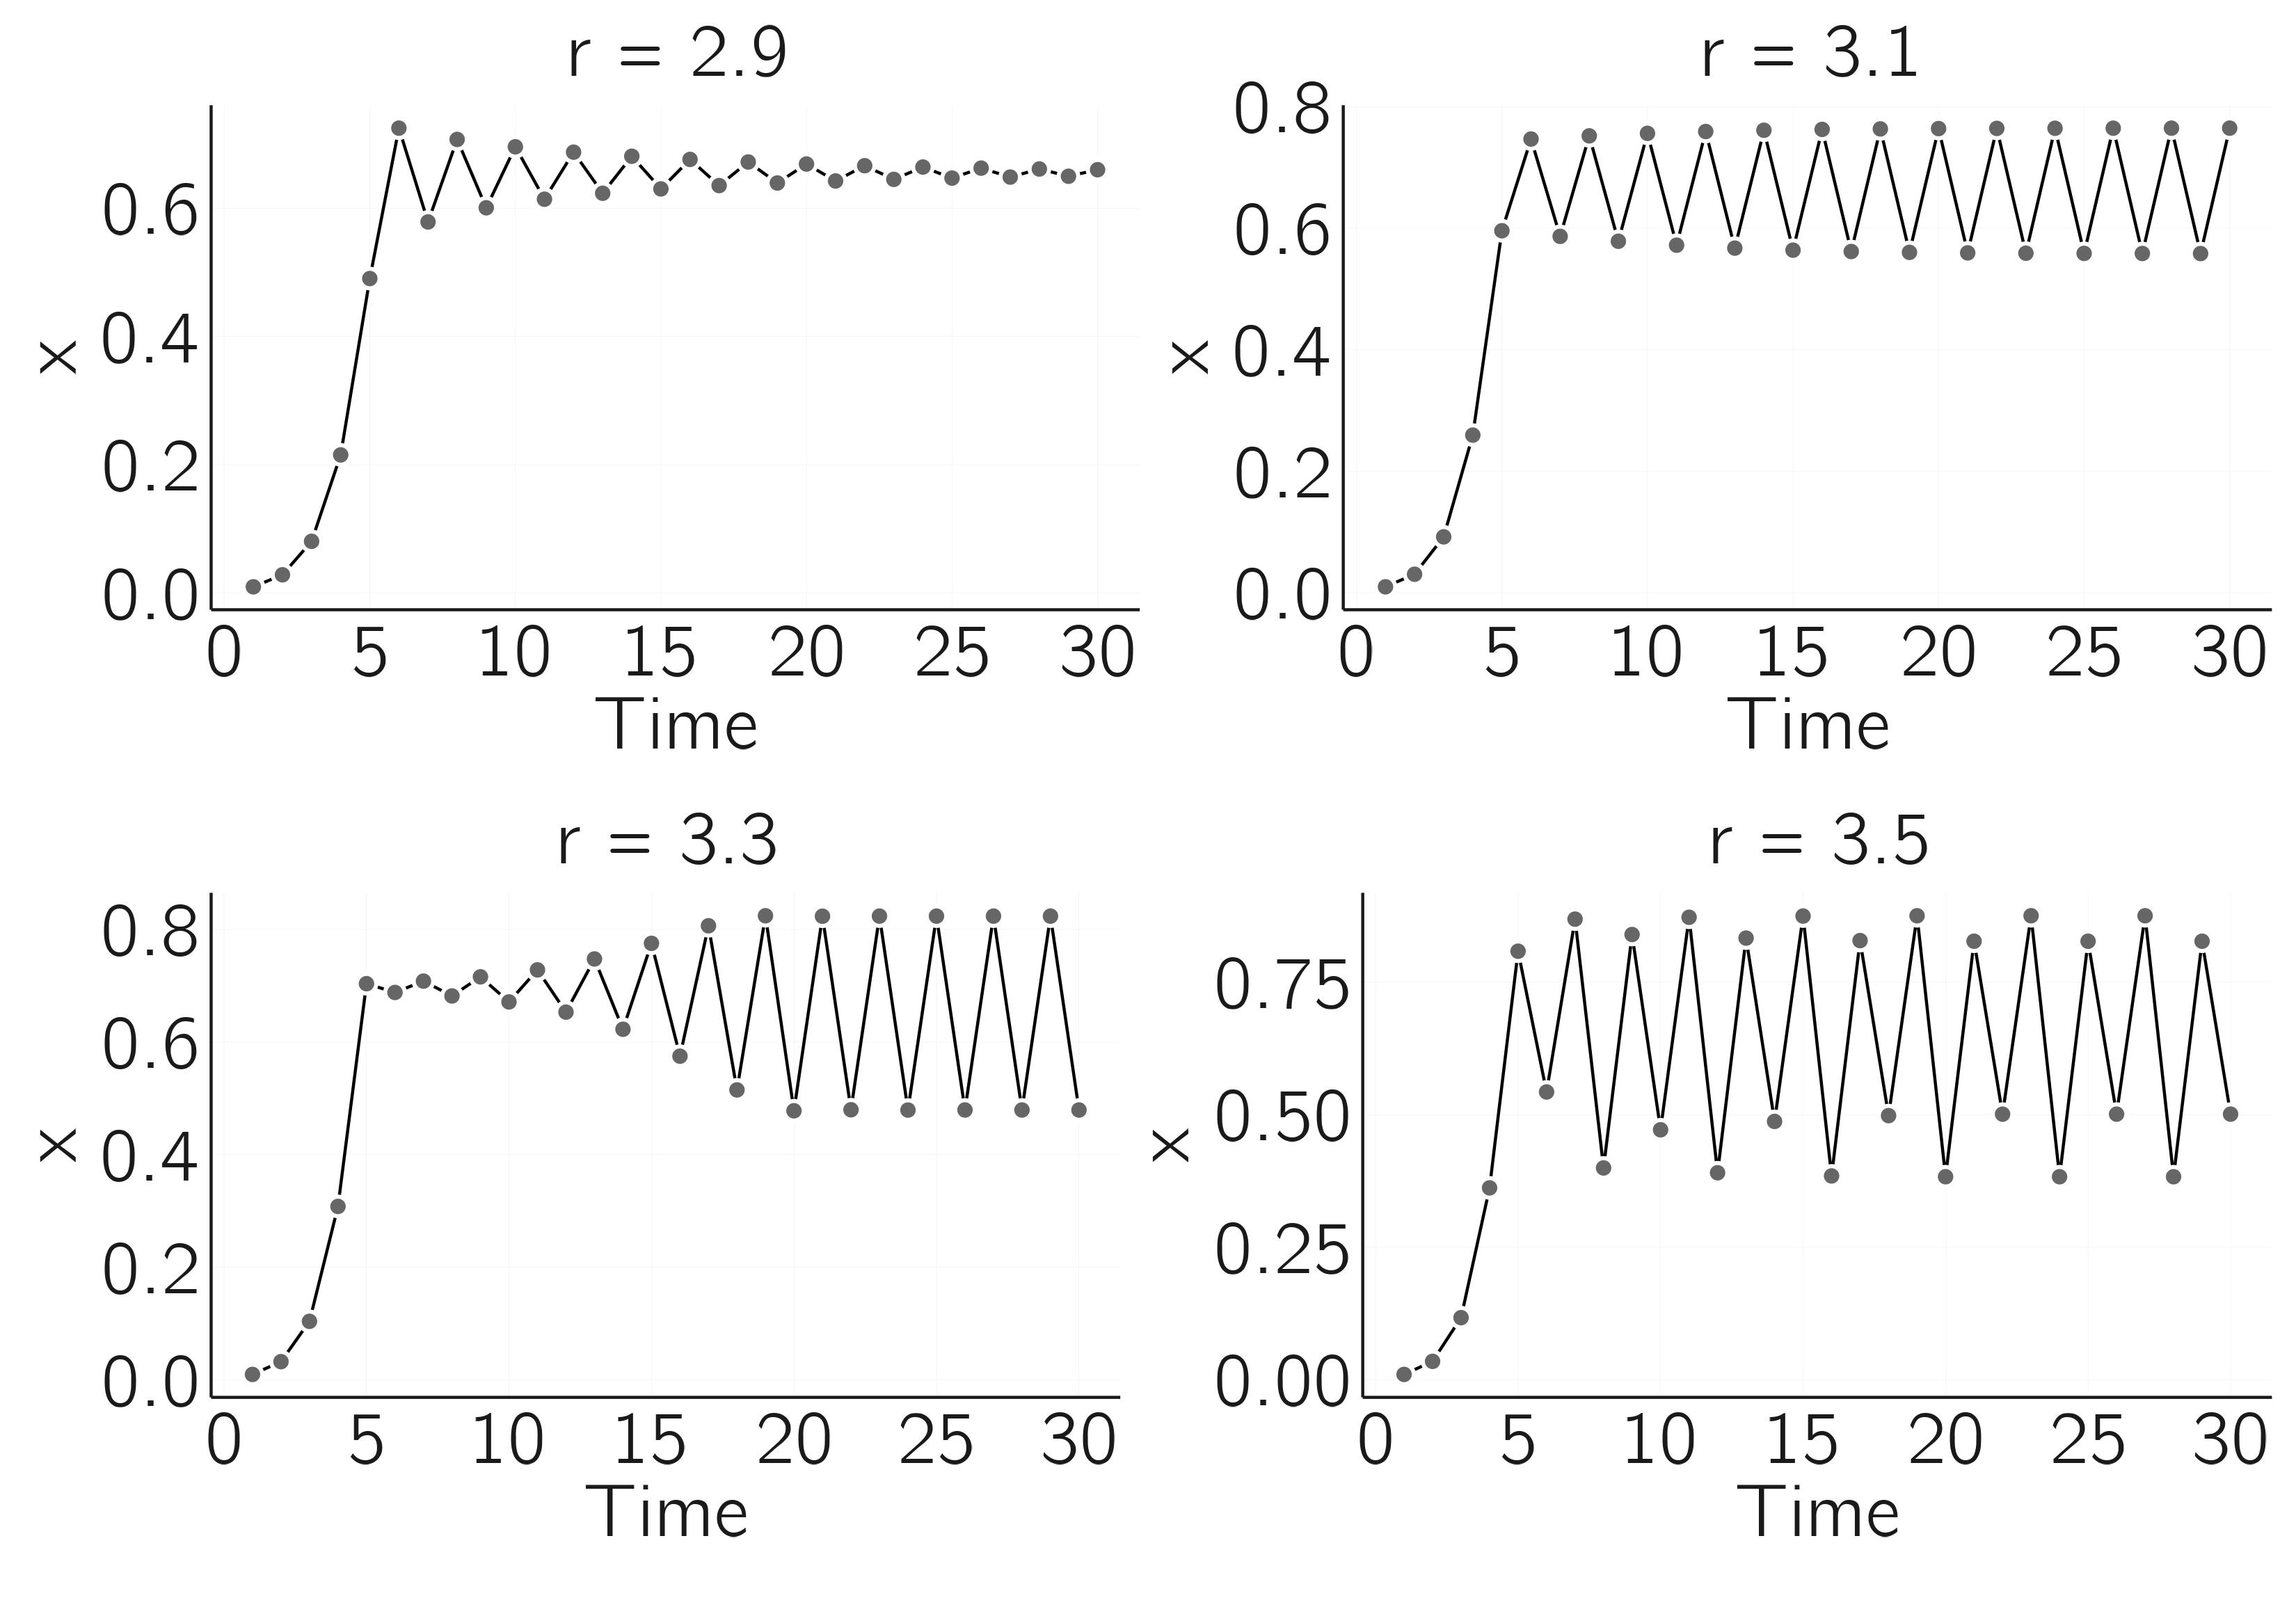
\includegraphics[width=13cm,height=\textheight]{media/ch2/fig-ch2-img4.jpg}

}

\caption{\label{fig-ch2-img4}Qualitative different behavior of the
logistic map for different values of \(r\).}

\end{figure}%

For \(r = 2.9\) we see that the series converges to the fixed point
\(\frac{1.9}{2.9} = .66,\) but in a process of over- and undershooting.
Between \(r = 3.1\) and \(r = 3.3\), a limit cycle of period 2 arises.
{\marginnote{\begin{footnotesize}In a limit cycle of period 2, the
population oscillates between two values.\end{footnotesize}}} For
\(r = 3.5\) this becomes even more remarkable, and we see a limit cycle
of period 4. For slightly larger values, we could get cycles with higher
periods.

It has been claimed that these limit cycles occur in real population
dynamics (Hassell, Lawton, and May 1976). Intuitively, it can be
understood as a process of over- and undershooting, which dampens out
for \(r\) a little below 3, but not for \(r > 3\).

\section{Chaos}\label{sec-Chaos}

If we increase \(r\) even further, the doubling of the periods changes
to even stranger behavior. Figure~\ref{fig-ch2-img4} shows what the time
series looks for \(r = 4\).

\begin{figure}

\centering{

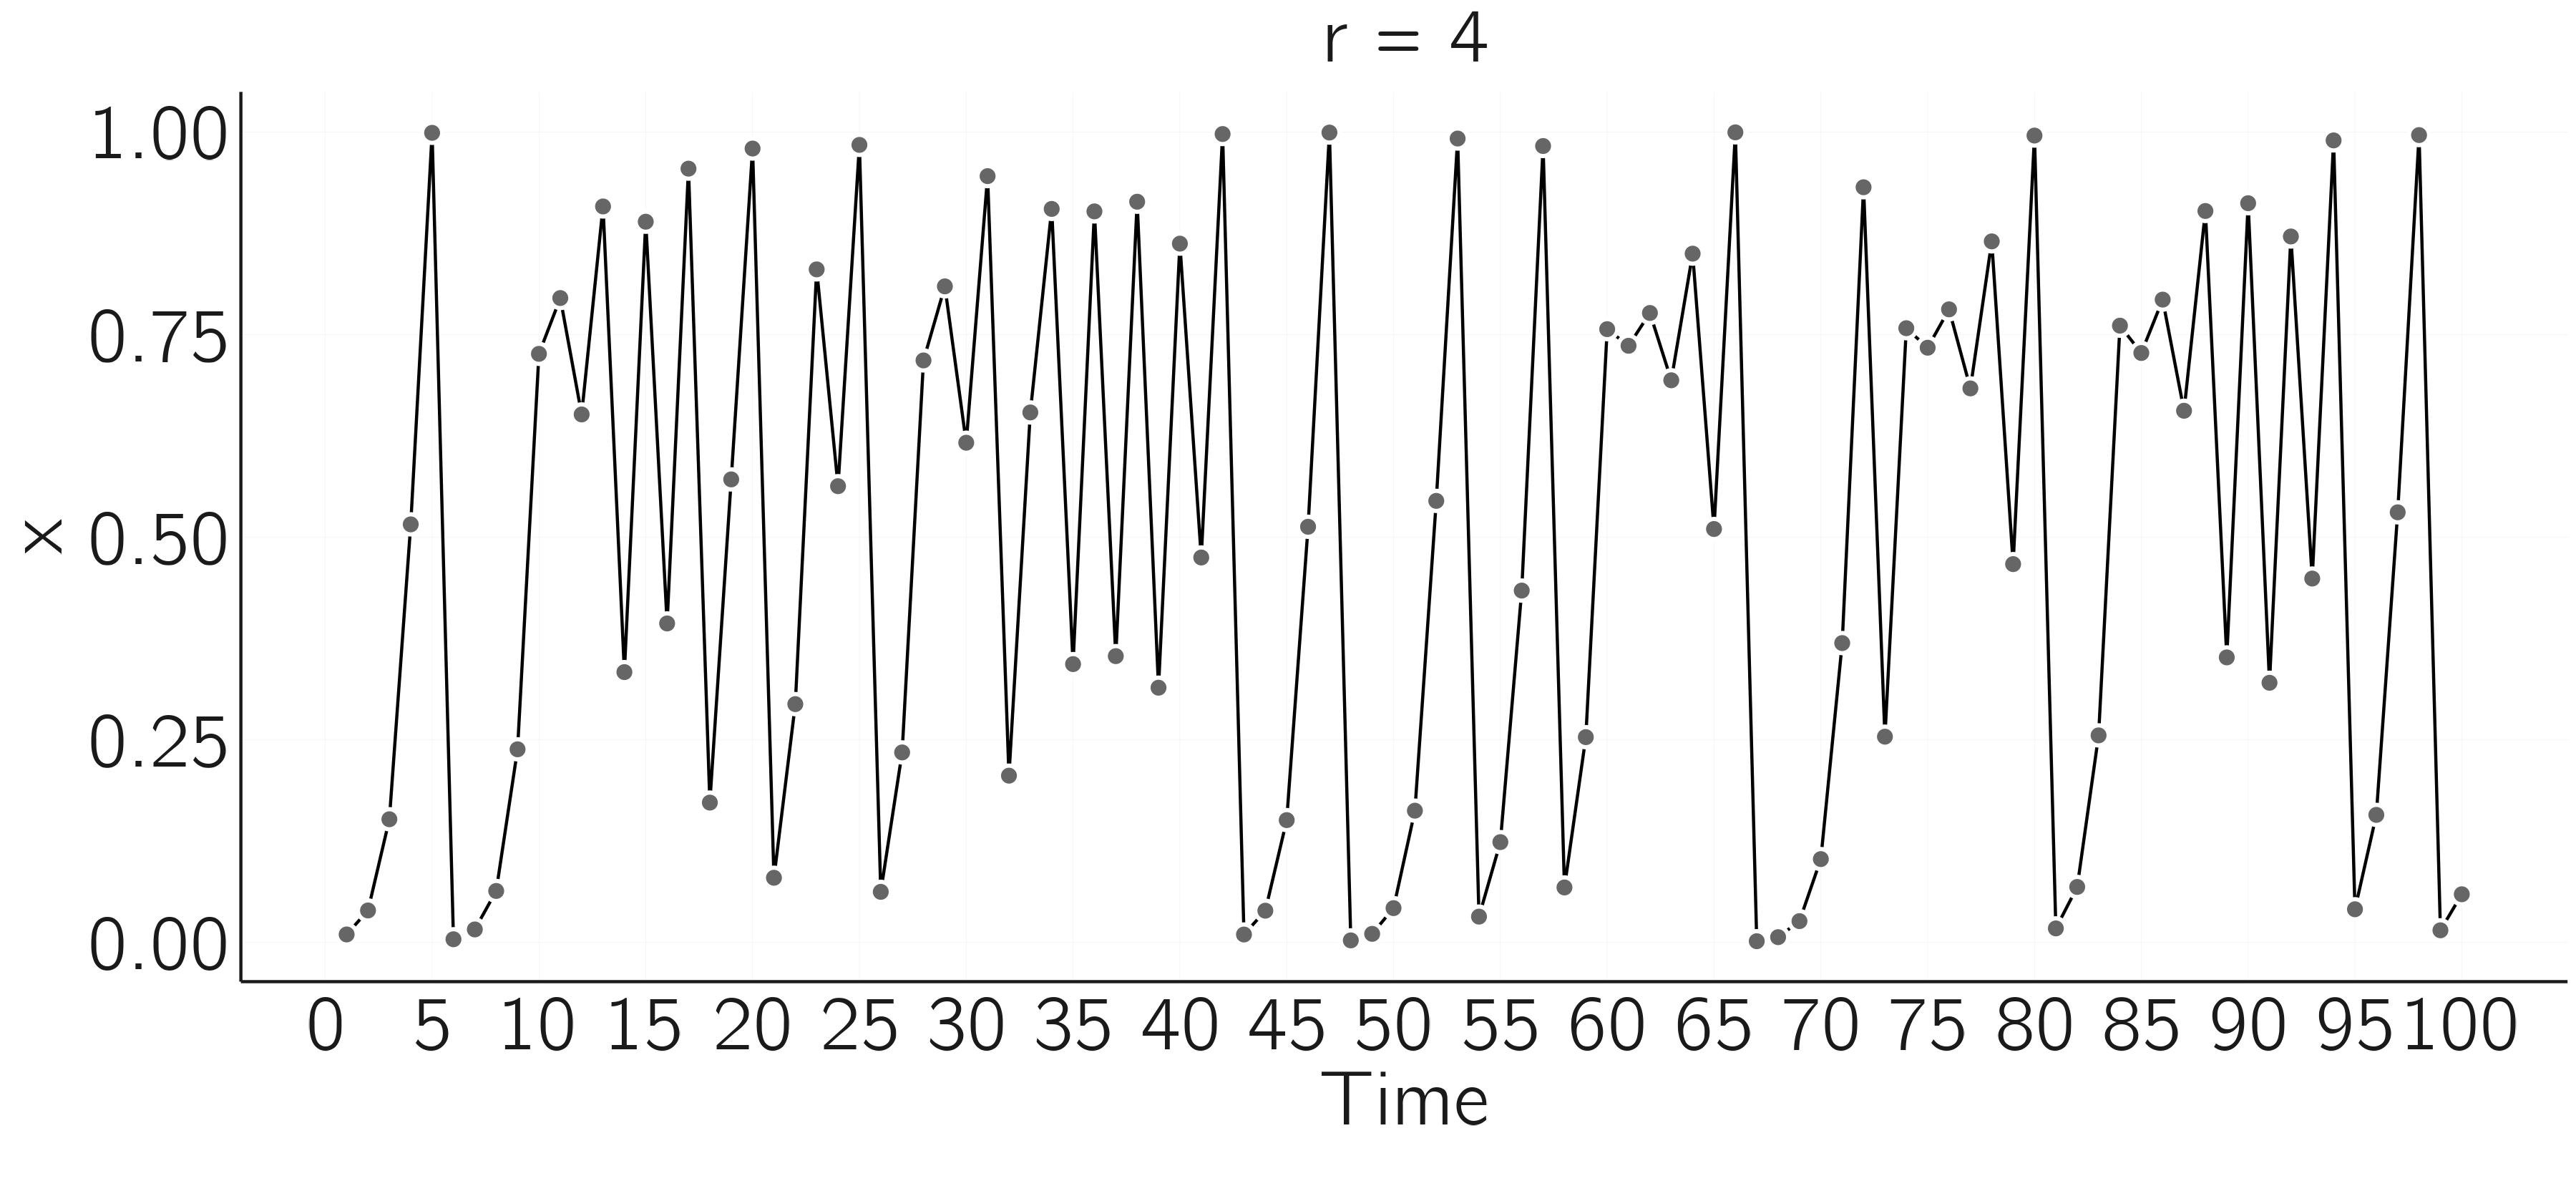
\includegraphics[width=10cm,height=\textheight]{media/ch2/fig-ch2-img5.jpg}

}

\caption{\label{fig-ch2-img5}Chaos for \(r = 4\).}

\end{figure}%

There seems to be no regularity. This is what we call deterministic
chaos. This time series is unpredictable, even though we know the
equation and the system is deterministic. What exactly do we mean by
this? Let me illustrate.

\begin{Shaded}
\begin{Highlighting}[]
\NormalTok{r }\OtherTok{\textless{}{-}} \DecValTok{4}\NormalTok{;  n }\OtherTok{\textless{}{-}} \DecValTok{50}\NormalTok{; x }\OtherTok{\textless{}{-}} \FunctionTok{rep}\NormalTok{(}\DecValTok{0}\NormalTok{,n)}
\NormalTok{x[}\DecValTok{1}\NormalTok{] }\OtherTok{\textless{}{-}}\NormalTok{ .}\DecValTok{001}
\ControlFlowTok{for}\NormalTok{ (i }\ControlFlowTok{in} \DecValTok{1}\SpecialCharTok{:}\NormalTok{(n }\SpecialCharTok{{-}} \DecValTok{1}\NormalTok{))}
\NormalTok{  x[i }\SpecialCharTok{+} \DecValTok{1}\NormalTok{] }\OtherTok{\textless{}{-}}\NormalTok{ r }\SpecialCharTok{*}\NormalTok{ x[i] }\SpecialCharTok{*}\NormalTok{ (}\DecValTok{1} \SpecialCharTok{{-}}\NormalTok{ x[i])}
\FunctionTok{plot}\NormalTok{(x, }\AttributeTok{type =} \StringTok{\textquotesingle{}l\textquotesingle{}}\NormalTok{, }\AttributeTok{xlab =} \StringTok{\textquotesingle{}time\textquotesingle{}}\NormalTok{, }\AttributeTok{bty =} \StringTok{\textquotesingle{}n\textquotesingle{}}\NormalTok{)}
\NormalTok{x[}\DecValTok{1}\NormalTok{] }\OtherTok{\textless{}{-}}\NormalTok{ .}\DecValTok{0010001}
\CommentTok{\# restart with sightly different initial state}
\ControlFlowTok{for}\NormalTok{ (i }\ControlFlowTok{in} \DecValTok{1}\SpecialCharTok{:}\NormalTok{(n }\SpecialCharTok{{-}} \DecValTok{1}\NormalTok{))}
\NormalTok{  x[i }\SpecialCharTok{+} \DecValTok{1}\NormalTok{] }\OtherTok{\textless{}{-}}\NormalTok{ r }\SpecialCharTok{*}\NormalTok{ x[i] }\SpecialCharTok{*}\NormalTok{ (}\DecValTok{1} \SpecialCharTok{{-}}\NormalTok{ x[i])}
\FunctionTok{lines}\NormalTok{(x, }\AttributeTok{col =} \StringTok{\textquotesingle{}red\textquotesingle{}}\NormalTok{)}
\end{Highlighting}
\end{Shaded}

\begin{figure}

\centering{

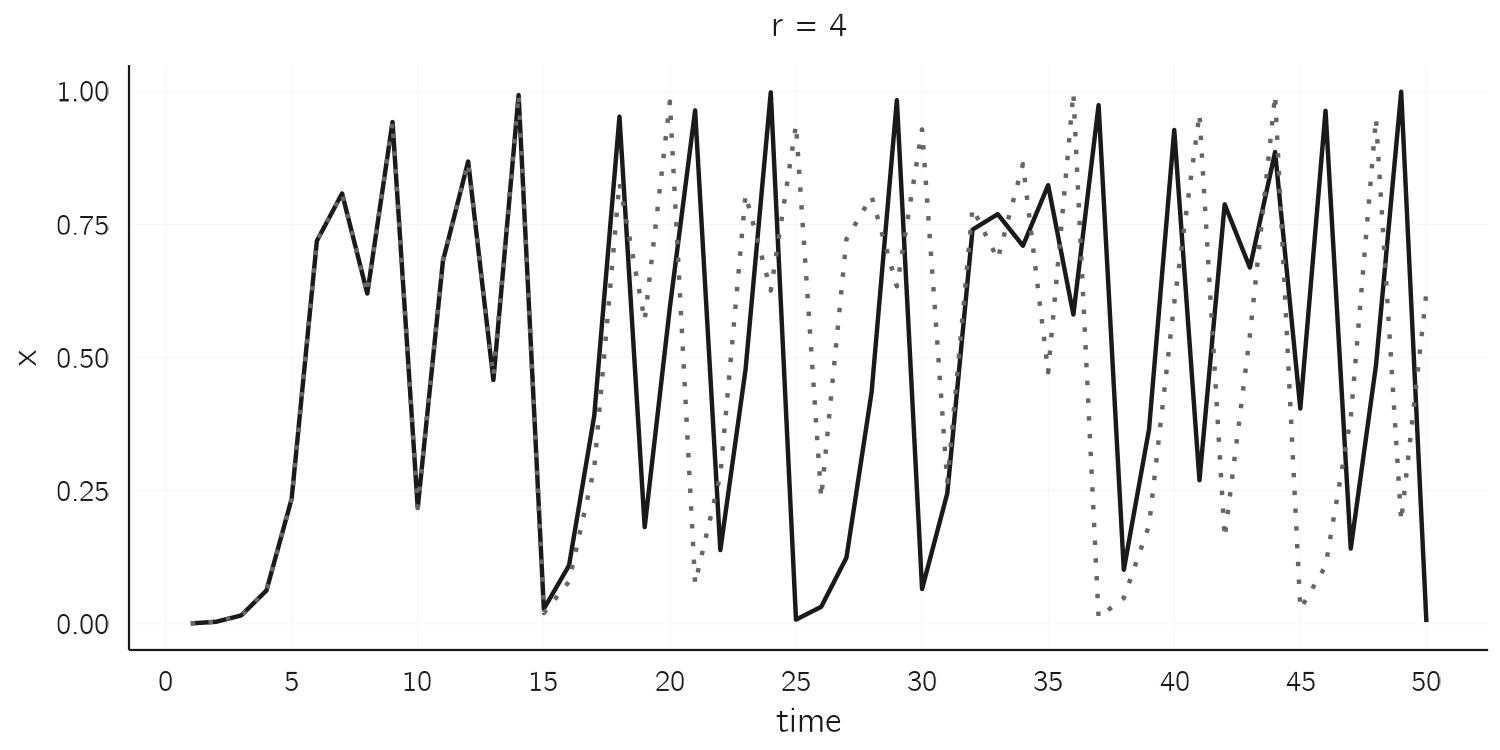
\includegraphics[width=10cm,height=\textheight]{media/ch2/fig-ch2-img6.jpg}

}

\caption{\label{fig-ch2-img6}The butterfly effect: A small difference in
initial state causes divergence in the long run.}

\end{figure}%

We can see that a run with a slightly different initial value will at
first follow the same path, but then it will diverge sharply
(figure~\ref{fig-ch2-img6}). A tiny perturbation (the butterfly flapping
its wings) propagates through the system and dramatically changes the
long-term course of the system.

{\marginnote{\begin{footnotesize}This is why long-term weather
prediction will never be possible, even if we develop much more precise
mathematical models, take more intensive and more accurate measurements,
and use more powerful computers.\end{footnotesize}}} Note that some
uncertainty about the exact value of the initial state is always
inevitable. Suppose we have an equation like the logistic map for
temperature in the weather system, and this equation perfectly describes
that system. To make a prediction, we need to feed the current
temperature into the computer. But we cannot measure temperature with
infinite precision. And even if we could, we do not have a computer that
can handle numbers with an infinite number of digits. So, we make a
small error in setting the initial state, and this will always mess up
our long-term forecast. The weather turns out to be a chaotic system.
Sensitivity to initial conditions is a necessary and perhaps sufficient
condition for deterministic chaos. For a discussion on the definition of
chaos, I refer to Banks et al. (1992) and Broer and Takens (2010).

{\marginnote{\begin{footnotesize}The Lyapunov coefficient quantifies
chaos.\end{footnotesize}}} The idea of the Lyapunov coefficient is to
take two very close initial conditions with a difference of
\(\varepsilon\). In the next iteration, this difference might be
smaller, the same, or bigger. In the last case, the time series diverge,
which is typical for chaos. The Lyapunov coefficient is defined as:

\begin{equation}\phantomsection\label{eq-ch2-3}{
{\lambda_{L} = \lim_{n \rightarrow \infty}}{\frac{1}{n}}{\sum_{i}^{n}{\ln\left| f^{'}\left( X_{i} \right) \right|}}}\end{equation}

where \(f^{'}\left( X_{i} \right) = r - 2rX_{i}\) for the logistic map
and \(\lambda_{L} > 0\) indicates chaos. You may verify in a simulation
that \(\lambda_{L} > 0\) for \(r = 4\), indicating chaos.

\section{Phase plot and bifurcation
diagrams}\label{sec-Phase-plot-and-bifurcation-diagrams}

Equation~\ref{eq-ch2-2} is very simple. It is just one equation, a
deterministic difference equation specifying how \(X_{t + 1}\) depends
on \(X_{t}\), but the variety of behavior is astonishing. One way to
better understand its behavior is to use phase plots.
{\marginnote{\begin{footnotesize}A phase plot is a graphical
representation of the relationship between two or more variables that
change over time.\end{footnotesize}}} In one-dimensional systems we plot
\(X_{t}\) against \(X_{t + 1}\) (see figure~\ref{fig-ch2-img7}). The
code for this figure is:

\begin{Shaded}
\begin{Highlighting}[]
\FunctionTok{layout}\NormalTok{(}\FunctionTok{matrix}\NormalTok{(}\DecValTok{1}\SpecialCharTok{:}\DecValTok{6}\NormalTok{,}\DecValTok{2}\NormalTok{,}\DecValTok{3}\NormalTok{))}
\NormalTok{r }\OtherTok{\textless{}{-}} \FloatTok{3.3}\NormalTok{; n }\OtherTok{\textless{}{-}} \DecValTok{200}\NormalTok{; x }\OtherTok{\textless{}{-}} \FunctionTok{rep}\NormalTok{(}\DecValTok{0}\NormalTok{,n)}
\NormalTok{x[}\DecValTok{1}\NormalTok{] }\OtherTok{\textless{}{-}}\NormalTok{ .}\DecValTok{001}
\ControlFlowTok{for}\NormalTok{(i }\ControlFlowTok{in} \DecValTok{1}\SpecialCharTok{:}\NormalTok{(n}\DecValTok{{-}1}\NormalTok{)) x[i}\SpecialCharTok{+}\DecValTok{1}\NormalTok{] }\OtherTok{=}\NormalTok{ r}\SpecialCharTok{*}\NormalTok{x[i]}\SpecialCharTok{*}\NormalTok{(}\DecValTok{1}\SpecialCharTok{{-}}\NormalTok{x[i])}
\NormalTok{x }\OtherTok{\textless{}{-}}\NormalTok{ x[}\SpecialCharTok{{-}}\DecValTok{1}\SpecialCharTok{:{-}}\DecValTok{100}\NormalTok{]}
\FunctionTok{plot}\NormalTok{(x,}\AttributeTok{type=}\StringTok{\textquotesingle{}l\textquotesingle{}}\NormalTok{,}\AttributeTok{xlab=}\StringTok{\textquotesingle{}time\textquotesingle{}}\NormalTok{,}\AttributeTok{bty=}\StringTok{\textquotesingle{}n\textquotesingle{}}\NormalTok{, }\AttributeTok{main=}\FunctionTok{paste}\NormalTok{(}\StringTok{\textquotesingle{}r = \textquotesingle{}}\NormalTok{,r),}
     \AttributeTok{ylim=}\DecValTok{0}\SpecialCharTok{:}\DecValTok{1}\NormalTok{,}\AttributeTok{cex.main=}\DecValTok{2}\NormalTok{) }
\FunctionTok{plot}\NormalTok{(x[}\SpecialCharTok{{-}}\FunctionTok{length}\NormalTok{(x)],x[}\SpecialCharTok{{-}}\DecValTok{1}\NormalTok{],}\AttributeTok{xlim=}\DecValTok{0}\SpecialCharTok{:}\DecValTok{1}\NormalTok{,}\AttributeTok{ylim=}\DecValTok{0}\SpecialCharTok{:}\DecValTok{1}\NormalTok{,}\AttributeTok{xlab=}\StringTok{\textquotesingle{}Xt\textquotesingle{}}\NormalTok{,}\AttributeTok{ylab=}\StringTok{\textquotesingle{}Xt+1\textquotesingle{}}\NormalTok{,}\AttributeTok{bty=}\StringTok{\textquotesingle{}n\textquotesingle{}}\NormalTok{)}
\NormalTok{r }\OtherTok{\textless{}{-}} \DecValTok{4}\NormalTok{; x[}\DecValTok{1}\NormalTok{] }\OtherTok{\textless{}{-}}\NormalTok{ .}\DecValTok{001}\NormalTok{;}
\ControlFlowTok{for}\NormalTok{(i }\ControlFlowTok{in} \DecValTok{1}\SpecialCharTok{:}\NormalTok{(n}\DecValTok{{-}1}\NormalTok{)) x[i}\SpecialCharTok{+}\DecValTok{1}\NormalTok{] }\OtherTok{\textless{}{-}}\NormalTok{ r}\SpecialCharTok{*}\NormalTok{x[i]}\SpecialCharTok{*}\NormalTok{(}\DecValTok{1}\SpecialCharTok{{-}}\NormalTok{x[i])}
\NormalTok{x }\OtherTok{\textless{}{-}}\NormalTok{ x[}\SpecialCharTok{{-}}\DecValTok{1}\SpecialCharTok{:{-}}\DecValTok{100}\NormalTok{]}
\FunctionTok{plot}\NormalTok{(x,}\AttributeTok{type=}\StringTok{\textquotesingle{}l\textquotesingle{}}\NormalTok{,}\AttributeTok{xlab=}\StringTok{\textquotesingle{}time\textquotesingle{}}\NormalTok{,}\AttributeTok{bty=}\StringTok{\textquotesingle{}n\textquotesingle{}}\NormalTok{,}\AttributeTok{main=}\FunctionTok{paste}\NormalTok{(}\StringTok{\textquotesingle{}r = \textquotesingle{}}\NormalTok{,r),}\AttributeTok{cex.main=}\DecValTok{2}\NormalTok{) }
\FunctionTok{plot}\NormalTok{(x[}\SpecialCharTok{{-}}\FunctionTok{length}\NormalTok{(x)],x[}\SpecialCharTok{{-}}\DecValTok{1}\NormalTok{],}\AttributeTok{xlim=}\DecValTok{0}\SpecialCharTok{:}\DecValTok{1}\NormalTok{,}\AttributeTok{ylim=}\DecValTok{0}\SpecialCharTok{:}\DecValTok{1}\NormalTok{,}\AttributeTok{xlab=}\StringTok{\textquotesingle{}Xt\textquotesingle{}}\NormalTok{,}\AttributeTok{ylab=}\StringTok{\textquotesingle{}Xt+1\textquotesingle{}}\NormalTok{,}\AttributeTok{bty=}\StringTok{\textquotesingle{}n\textquotesingle{}}\NormalTok{)}
\NormalTok{x }\OtherTok{\textless{}{-}} \FunctionTok{runif}\NormalTok{(}\DecValTok{200}\NormalTok{,}\DecValTok{0}\NormalTok{,}\DecValTok{1}\NormalTok{)}
\NormalTok{x }\OtherTok{\textless{}{-}}\NormalTok{ x[}\SpecialCharTok{{-}}\DecValTok{1}\SpecialCharTok{:{-}}\DecValTok{100}\NormalTok{]}
\FunctionTok{plot}\NormalTok{(x,}\AttributeTok{type=}\StringTok{\textquotesingle{}l\textquotesingle{}}\NormalTok{,}\AttributeTok{xlab=}\StringTok{\textquotesingle{}time\textquotesingle{}}\NormalTok{,}\AttributeTok{bty=}\StringTok{\textquotesingle{}n\textquotesingle{}}\NormalTok{,}\AttributeTok{main=}\StringTok{\textquotesingle{}random noise\textquotesingle{}}\NormalTok{,}\AttributeTok{cex.main=}\DecValTok{2}\NormalTok{) }
\FunctionTok{plot}\NormalTok{(x[}\SpecialCharTok{{-}}\FunctionTok{length}\NormalTok{(x)],x[}\SpecialCharTok{{-}}\DecValTok{1}\NormalTok{],}\AttributeTok{xlim=}\DecValTok{0}\SpecialCharTok{:}\DecValTok{1}\NormalTok{,}\AttributeTok{ylim=}\DecValTok{0}\SpecialCharTok{:}\DecValTok{1}\NormalTok{,}\AttributeTok{xlab=}\StringTok{\textquotesingle{}Xt\textquotesingle{}}\NormalTok{,}\AttributeTok{ylab=}\StringTok{\textquotesingle{}Xt+1\textquotesingle{}}\NormalTok{,}\AttributeTok{bty=}\StringTok{\textquotesingle{}n\textquotesingle{}}\NormalTok{)}
\end{Highlighting}
\end{Shaded}

\begin{figure}

\centering{

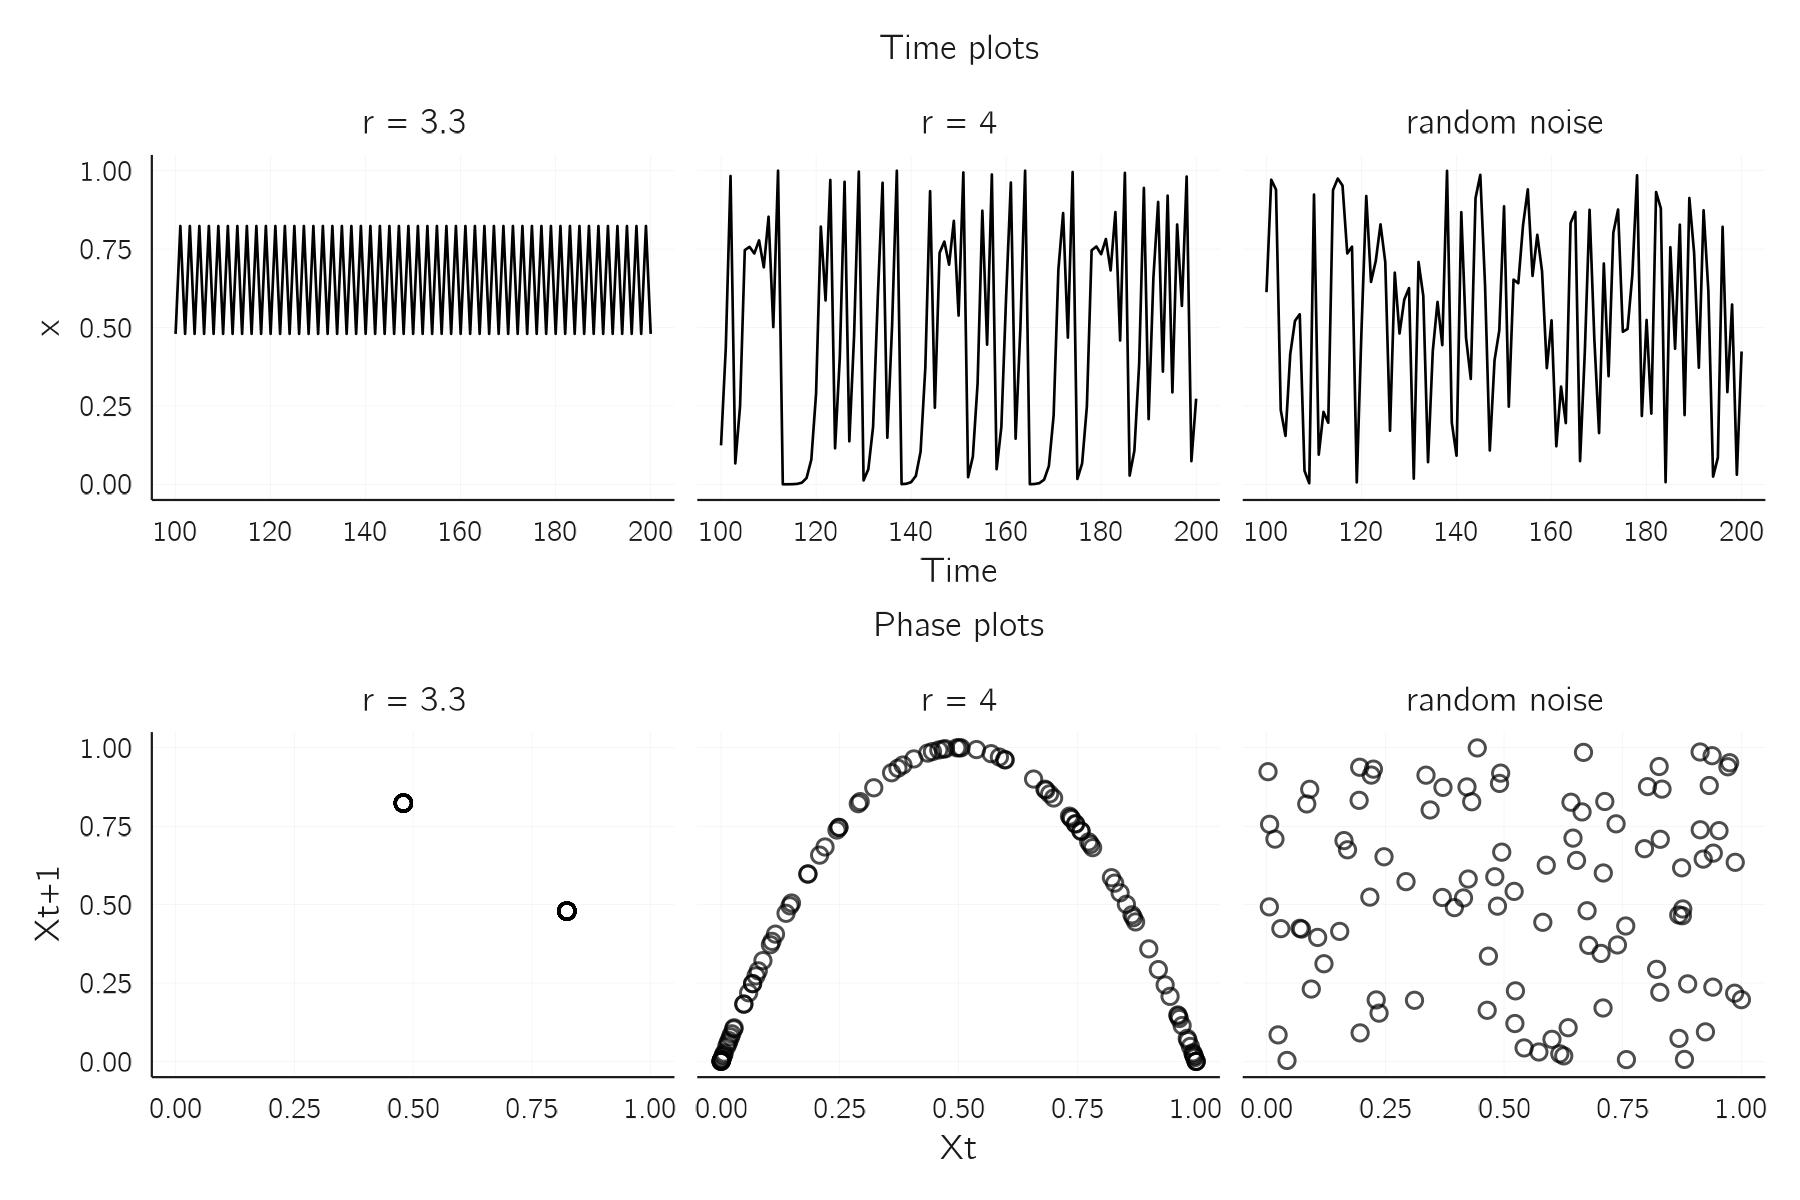
\includegraphics[width=13cm,height=\textheight]{media/ch2/fig-ch2-img7.jpg}

}

\caption{\label{fig-ch2-img7}Time (top) and phase (bottom) plots for
three cases. Chaos and random noise can be distinguished using the phase
plots.}

\end{figure}%

The top figures are time plots, and the lower figures are phase plots.
The first column shows a limit cycle of period 2, the second
deterministic chaos, and the third noise generated from a uniform
distribution. Although the time series of the second and third cases
look similar, the phase diagram reveals hidden structure in the chaos
time series. Phase plots can help us to distinguish chaos from noise.

The second useful graph is the bifurcation graph.
{\marginnote{\begin{footnotesize}A bifurcation graph is a diagram that
shows how the qualitative behavior of a system changes, for example,
from stable to chaotic, when one of its parameters
changes.\end{footnotesize}}} In case of the logistic map, it summarizes
the equilibrium behavior for different values of \(r\) in one figure.
The idea is to plot the equilibria as y-values for a range of
\(r\)-values on the x-axis. This means that if we take a low \(r\) value
\((r < 1)\), we will only plot 0s, as only \(X^{*} = 0\) is a stable
fixed point. Between 1 and 3, we will also see one fixed point equal to
\((r - 1)/r\). For \(r = 3.3\), we expect to see two points as the
attractor is a limit cycle with period 2. For higher \(r\) we get chaos.
How does this all look?

It is actually a good challenge to program this yourself. The trick is
to create time series for a range of values of \(r\), delete the first
part of this series (we only want the equilibrium behavior), and plot
these as y-values. So, if the logistic map has period 2 (\(r = 3.3\)),
we repeatedly plot only two points. For \(r = 4\) we get the whole chaos
band.

A clever way to do this is to use the \texttt{sapply} function in R.

\begin{Shaded}
\begin{Highlighting}[]
\FunctionTok{layout}\NormalTok{(}\DecValTok{1}\NormalTok{)}
\NormalTok{f }\OtherTok{\textless{}{-}} \ControlFlowTok{function}\NormalTok{(r, x, n, m)\{}
\NormalTok{  x }\OtherTok{\textless{}{-}} \FunctionTok{rep}\NormalTok{(x,n)}
  \ControlFlowTok{for}\NormalTok{(i }\ControlFlowTok{in} \DecValTok{1}\SpecialCharTok{:}\NormalTok{(n}\DecValTok{{-}1}\NormalTok{)) x[i}\SpecialCharTok{+}\DecValTok{1}\NormalTok{] }\OtherTok{\textless{}{-}}\NormalTok{ r}\SpecialCharTok{*}\NormalTok{x[i]}\SpecialCharTok{*}\NormalTok{(}\DecValTok{1}\SpecialCharTok{{-}}\NormalTok{x[i])}
\NormalTok{  x[}\FunctionTok{c}\NormalTok{((n}\SpecialCharTok{{-}}\NormalTok{m)}\SpecialCharTok{:}\NormalTok{n)] }\CommentTok{\# only return last m iterations}
\NormalTok{\}}
\NormalTok{r.range }\OtherTok{\textless{}{-}} \FunctionTok{seq}\NormalTok{(}\DecValTok{0}\NormalTok{, }\FloatTok{2.5}\NormalTok{, }\AttributeTok{by=}\FloatTok{0.01}\NormalTok{) }
\NormalTok{r.range }\OtherTok{\textless{}{-}} \FunctionTok{c}\NormalTok{(r.range,}\FunctionTok{seq}\NormalTok{(}\FloatTok{2.5}\NormalTok{, }\DecValTok{4}\NormalTok{, }\AttributeTok{by=}\FloatTok{0.001}\NormalTok{)) }
\NormalTok{n }\OtherTok{\textless{}{-}} \DecValTok{200}\NormalTok{; m }\OtherTok{\textless{}{-}}\DecValTok{100} 
\NormalTok{equilibria }\OtherTok{\textless{}{-}} \FunctionTok{as.vector}\NormalTok{(}\FunctionTok{sapply}\NormalTok{(r.range, f,  }\AttributeTok{x=}\FloatTok{0.1}\NormalTok{, }\AttributeTok{n=}\NormalTok{n, }\AttributeTok{m=}\NormalTok{m}\DecValTok{{-}1}\NormalTok{))}
\NormalTok{r }\OtherTok{\textless{}{-}} \FunctionTok{sort}\NormalTok{(}\FunctionTok{rep}\NormalTok{(r.range, m))}
\FunctionTok{plot}\NormalTok{(equilibria }\SpecialCharTok{\textasciitilde{}}\NormalTok{ r, }\AttributeTok{pch=}\DecValTok{19}\NormalTok{,}\AttributeTok{cex=}\NormalTok{.}\DecValTok{01}\NormalTok{,}\AttributeTok{bty=}\StringTok{\textquotesingle{}n\textquotesingle{}}\NormalTok{)}
\end{Highlighting}
\end{Shaded}

This results in figure~\ref{fig-ch2-img8}. We see indeed fixed stable
points for \(r < 3\), the period doubling of the limit cycles for
\(r > 3\), followed by chaos.

\begin{figure}

\centering{

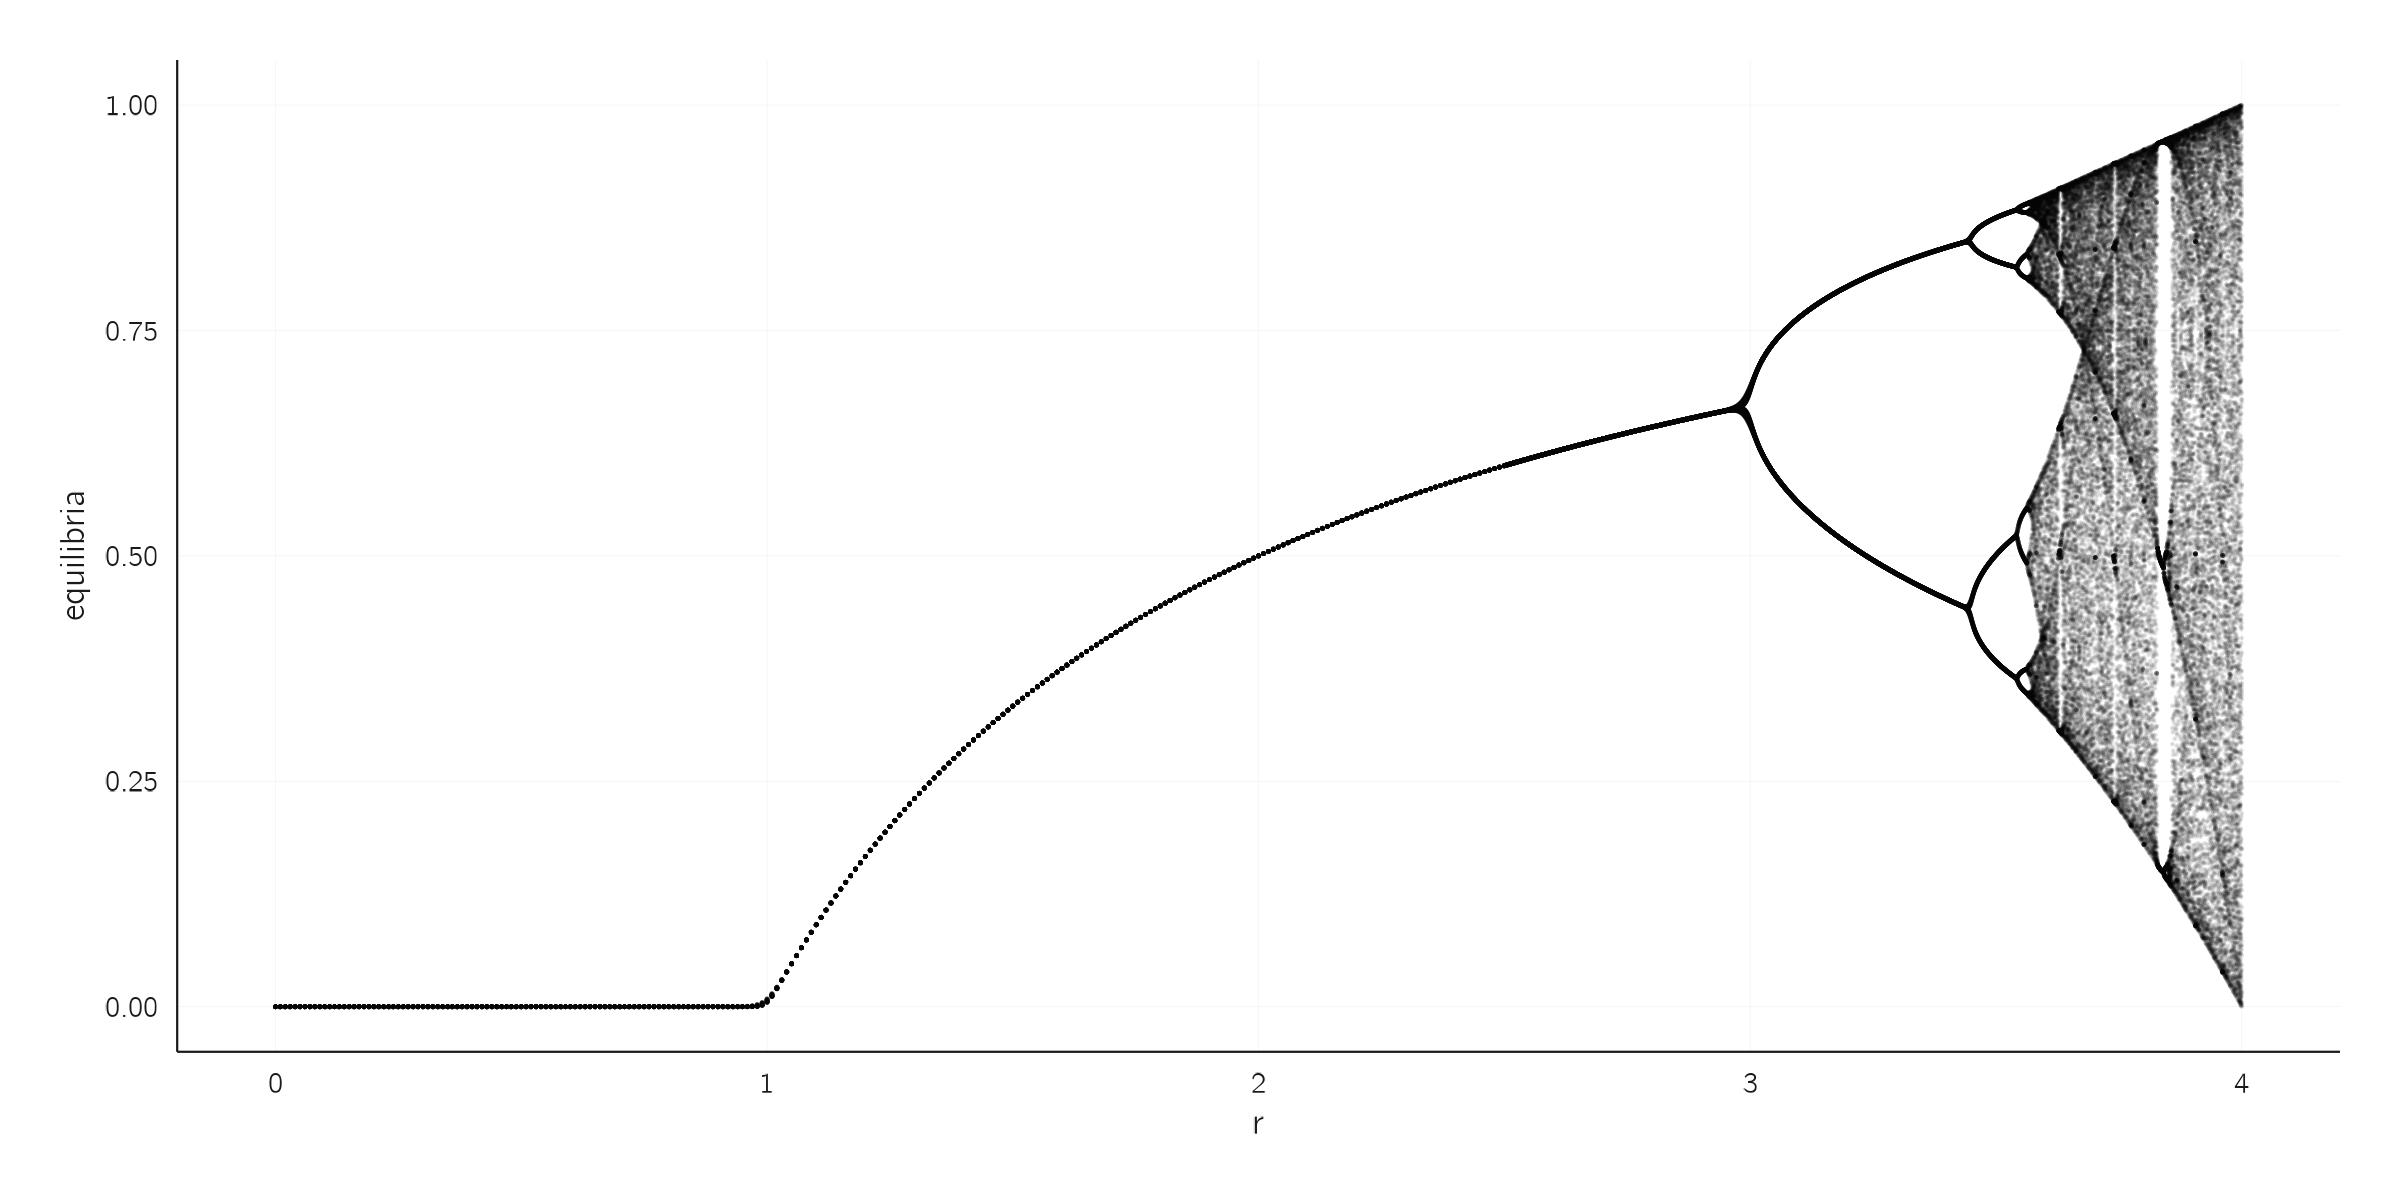
\includegraphics[width=13cm,height=\textheight]{media/ch2/fig-ch2-img8.jpg}

}

\caption{\label{fig-ch2-img8}The bifurcation diagram of the logistic
map.}

\end{figure}%

Fractals are a recurring phenomenon in many chaotic maps.
{\marginnote{\begin{footnotesize}Fractals are figures in which certain
patterns reappear when we zoom in on the figure, and this happens again
and again when we zoom in farther.\end{footnotesize}}} You can see the
fractal nature of the logistic map by zooming in on the interval of
\(r\) between 3.83 and 3.86 (see exercise 2). The three equilibria in
the limit cycle split again into period doubling cycles, as we saw in
the overall plot between \(r\) in 3 and 3.5.

One famous result on this period doubling route to chaos is the
Feigenbaum constant. The ratios of distances between consecutive period
doubling points (e.g., the distance between first and second divided by
the distance between the second and third point) converge to a value of
approximately 4.6692. The amazing thing is that this constant is the
same for any unimodal map.

\section{What did we learn?}\label{sec-What-did-we-learn}

I find these results stunning. I note again that the generating function
is deceptively simple, but its behavior is utterly complex and
beautiful. Mathematicians have studied every detail of these plots, and
most of it is beyond my comprehension. The Wikipedia on the logistic map
will introduce you to some more advanced concepts, but for our purposes
the present introduction will suffice.

First. let's review the concepts we have already learned. The first is
the concept of equilibrium. The states of dynamical systems tend to
converge to certain values. The simplest of these is the fixed point.
Fixed points can be stable or unstable (more on this in the next
chapter). If we start a system exactly at its unstable fixed point (and
there is no noise in the system), it will stay there. But any small
perturbation will cause it to escape and move to the fixed stable point.

The bifurcation diagram summarizes this behavior and also shows how the
equilibria change when a control parameter changes. For example, at
\(r = 1\) we see a bifurcation in the logistic map. Initially 0 was the
stable fixed point and \((r - 1)/r\) was unstable. At \(r = 1\) this is
reversed. At \(r = 3\) we see another bifurcation when limit cycles
appear.

We have learned that there are all sorts of equilibria. The strangest
ones are called strange attractors, which are associated with
deterministic chaos. You can see them by making a phase diagram. Phase
diagrams for other famous maps are often stunning. The most famous is
the Mandelbrot set (look on the internet). There is an R blog about the
Mandelbrot set.\footnote{\url{https://www.r-bloggers.com/2017/06/the-mandelbrot-set-in-r-2/}.
  Be sure to check the Shiny app.} Simulation helps understanding!

The last thing we learned is that even if our world were deterministic
(it is not!), and we knew all the laws of motion (say, the logistic
map), and we knew initial states with enormous precision, the world
would still be unpredictable.

This statement needs some nuance. I have already mentioned that the
weather can be chaotic and unpredictable. But the weather is not always
so unpredictable. Sometimes longer forecasts are possible. But forecasts
beyond, say, 10 days seem out of reach. We also see in the logistic map
that when \(r\) is close to 4, the forecast suffers from the butterfly
effect, but for \(r = 2\) the time course is very predictable, even more
predictable than in many linear systems. This is because there is only
one stable fixed point (.5). The initial state does not matter: we
always end up at .5! {\marginnote{\begin{footnotesize}The logistic map
is either extremely predictable or extremely unpredictable depending on
the value of \(r\).\end{footnotesize}}}

\section{Other maps and fractals}\label{sec-Other-maps-and-fractals}

There are many accessible sources on chaos theory. As always, Wikipedia
is a great resource. It helps me a lot by actually doing things, that
is, doing computer simulations. One example is the Henon map, which
consists of two coupled difference equations:

\begin{equation}\phantomsection\label{eq-ch2-4}{
\begin{gathered}
X_{t + 1} = 1 - aX_{t}^{2} + Y_{t} \\
Y_{t + 1} = bX_{t} 
\end{gathered}
}\end{equation}

Using the code example from the logistic map, you should be able to
generate time series and a phase diagram for this model. Try to
reproduce the first image of the Wikipedia page on the Henon map. The
amazing three-dimensional bifurcation diagram may be more challenging.

Fractals are another topic for further study. Another look at Wikipedia
is recommended. Making your own fractals in R is made easy by the R blog
by Martin Stefan (2020).

\section{Detecting chaos in psychophysiological
data}\label{sec-Detecting-chaos-in-psychophysiological-data}

Chaos theory and the logistic map were popularized about fifty years
ago, and since then researchers have been looking for chaos in all kinds
of time series (Ayers 1997; Robertson and Combs 2014; G. K. Schiepek et
al. 2017). One idea behind this work is the hypothesis that chaos might
be healthy (Pool 1989) or helpful. It would be helpful in learning
algorithms, such as neural networks, to prevent getting stuck in local
minima (Bertschinger and Natschläger 2004). My very first publication
was about chaos in neural networks (van der Maas, Verschure, and
Molenaar 1990).

There are many techniques for chaos detection in times series. However,
these empirical signals are inevitably contaminated with noise (Rosso et
al. 2007). One example is the computation of Lyapunov exponents,
quantifying how small differences in initial conditions evolve over
time. A positive Lyapunov exponent indicates chaos, signifying
exponential divergence of trajectories, which is a hallmark of chaotic
systems. This method involves reconstructing the phase space from
time-series data and calculating the average exponential rate of
separation of trajectories. With the Lyapunov function in the package
DChaos, you can compute the Lyapunov coefficient for times series
generated with the logistic map. You may verify that for \(r = 4\), you
get the Lyapunov coefficient as computed with the derivative earlier.
{\marginnote{\begin{footnotesize}Chaos detection is an active area of
research, with new methods being proposed on a regular basis (Zanin
2022).\end{footnotesize}}} There are several packages available in R,
including new methods based on machine-learning techniques (Sandubete
and Escot 2021; Toker, Sommer, and D'Esposito 2020).

These methods generally require long time series. Many publications
appeared on the detection of chaos in psychophysiological data. Examples
are electroencephalogram (EEG) (Pritchard and Duke 1992) heartbeat
(Freitas et al. 2009), electromyogram (EMG) (Lei, Wang, and Feng 2001),
and eye movements (Harezlak and Kasprowski 2018). Reviews of these lines
of research are provided by Stam (2005), Kargarnovin et al. (2023), and
Garc and Pe (2015).

\section{Exercises}\label{sec-Exercises-ch2}

\begin{enumerate}
\def\labelenumi{\arabic{enumi})}
\item
  For \(r=3.5\), the logistic map iterates between four points. For
  which value(s) does it iterate between 8 points? (*)
\item
  Section~\ref{sec-Phase-plot-and-bifurcation-diagrams} shows the code
  to make a bifurcation plot. First, run this code and look at the
  bifurcation plot. In this plot, you can also zoom in by changing the
  interval between the \(r\)'s on the x-axis. Adjust the code by
  changing the \texttt{r.range} to \texttt{seq(3.4,\ 4,\ by=0.0001)},
  also change \texttt{cex\ =\ 0.01} to a lower value. Zoom in on the
  interval of \(r\) between 3.83 and 3.86. In this interval the chaos
  suddenly disappears and limit cycles with period 3 appear. Check this
  with a time-series plot for a particular value of \(r\). (*)
\item
  Reproduce the first image from the Henon map Wikipedia page. Provide
  your R code and figure (*).
\item
  Make the bifurcation diagram of the Ricker model (see Wikipedia).
  Provide your R code and figure. Why is this model considered a more
  realistic representation of population growth than the logistic map?
  (*)
\item
  Also reproduce the three-dimensional bifurcation diagram of the Henon
  map. (**)
\item
  Have a look at the definition of the Lyapunov coefficient in
  section~\ref{sec-Chaos}. Calculate this Lyapunov coefficient for the
  logistic map where \(r = 4\) using the Dchaos package in R. This
  coefficient can also be calculated manually using the derivative
  (equation~\ref{eq-ch2-3}). Do this and check that the coefficients are
  approximately equal. (**)
\item
  Use the Rmusic library (installed with\\
  \texttt{devtools::install\_github("keithmcnulty/Rmusic",\ build\_vignettes\ =\ TRUE)}
  to create a chaos sound machine. Make one for white noise too. Can you
  hear the difference? (**)
\item
  Find a paper on chaos detection in psychology or psychophysiology and
  summarize it in 300---400 words. (*)
\end{enumerate}

\bookmarksetup{startatroot}

\chapter{Transitions in complex systems}\label{sec-ch3}

\section{Introduction}\label{sec-Introduction-ch3}

My dissertation research was on Jean Piaget's stage theory of cognitive
development. These stages were separated by transitions. One such
transition should occur between the pre-operational and
concrete-operational stages. In the concrete-operational stage, children
learn logical, concrete physical rules about objects, such as weight,
height, and volume. The most famous test to distinguish between the two
stages is the conservation task.

There are many conservation tasks, but the setup is always the same. For
example, you show a child two equal balls of clay, ask for confirmation
that they weigh the same, roll one into a sausage shape, and then ask
again for confirmation of equal weight. A nonconserving child will now
claim that the longer sausage weighs more. One can also do this with two
rows of coins (spreading one row out) or two glasses of water (pouring
the water from one glass into a smaller longer glass). It is actually a
fascinating task to do with children between five and eight years old.

From the 1960s to the 1980s, this was a topic of major interest in
developmental psychology. A key question was whether there really was a
stage transition, and there was a lot of confusion about what a
transition actually was. It was my task to clarify this and to prove
Piaget's hypothesis. I think I succeeded in clarifying the question, but
whether I succeeded in proving the stage theory is debatable.\footnote{Learning
  a particular conservation task does seem to be rather sudden, but
  there could easily be two years between learning conservation of
  number and conservation of volume (Kreitler and Kreitler 1989). This
  is inconsistent with the stage theory.}

My PhD advisor Peter Molenaar had the idea to use catastrophe theory to
define the concept of a transition in a precise way, to use the
so-called catastrophe flags to test the hypothesis of a transition, and
also to fit a cusp model to the conservation data. It took me, with the
help of many people, more than 20 years to do all these steps (van der
Maas and Molenaar 1992; Jansen and van der Maas 2001; Dolan and van der
Maas 1998; Grasman, van der Maas, and Wagenmakers 2009).

What is catastrophe theory, what are these flags, and what is the cusp?
These are the first questions I will answer in this chapter. But this
chapter is also about statistics. You will learn how to fit a cusp model
to data. I will present a methodology for studying transitions in areas
where we do not have a mathematical description of the underlying
system. I will present examples from very different subfields of
psychology. Finally, I will discuss the criticisms that were made in
response to the hype around catastrophe theory about fifty years ago.
This is a long chapter, but I have tried to include only what is
necessary in order to make intelligent use of this approach. This
requires some basic understanding of the mathematics of catastrophe
theory, a good overview of the possibilities for testing cusp models,
and knowledge of the controversies from the early days of the
popularization of this theory.

\section{Examples of transitions}\label{sec-Examples-of-transitions}

In Chapter 1, section~\ref{sec-A-limited-number-of-equilibria}, I stated
that complex systems tend to be characterized by a limited number of
equilibria. As we saw in the Chapter 2, these equilibria can take many
different forms, but in this chapter, we consider only stable and
unstable fixed points. We are particularly interested in the case where
the configuration of stable and unstable points changes due to a smooth
change in some external variable, a control variable. In such a case a
discontinuous change or a (first-order) phase transition can occur. A
transition or tipping point is an intriguing property of complex
systems.

I call it an intriguing property because in the linear systems we are
used to, smooth changes in control variables lead to similar
(proportional) changes in behavior variables. We may see a big change in
some behavior, but this requires a big change in the controls. An
example would be the speed of your bike and the force you apply. But in
the case of fear or panic, this process is often nonlinear.
{\marginnote{\begin{footnotesize}If a smooth change in an independent or
control variable, such as the smell of smoke, leads to a sudden jump in
fear (e.g., panic), we are likely to be dealing with a phase
transition.\end{footnotesize}}}

A key physical example is the change in state of water. Between, say, 10
and 80 degrees Celsius, a smooth change in temperature results in only a
slight change in the liquid state of water. But if we change the
temperature very slowly, close to the thresholds of 0 or 100 degrees
Celsius, we see sudden phase transitions.

We saw something similar for the logistic map when \(r\) crossed the
boundary at \(r = 1\). However, this did not lead to a sudden change in
\(X^{*}\). This is often called a second-order phase transition, meaning
that the configuration of stable and unstable points changes, but there
is no discontinuous change in behavior
(figure~\ref{fig-ch3-img1-old-13}).\footnote{A related and very similar
  distinction is that between a subcritical bifurcation and a
  supercritical bifurcation.}

\begin{figure}

\centering{

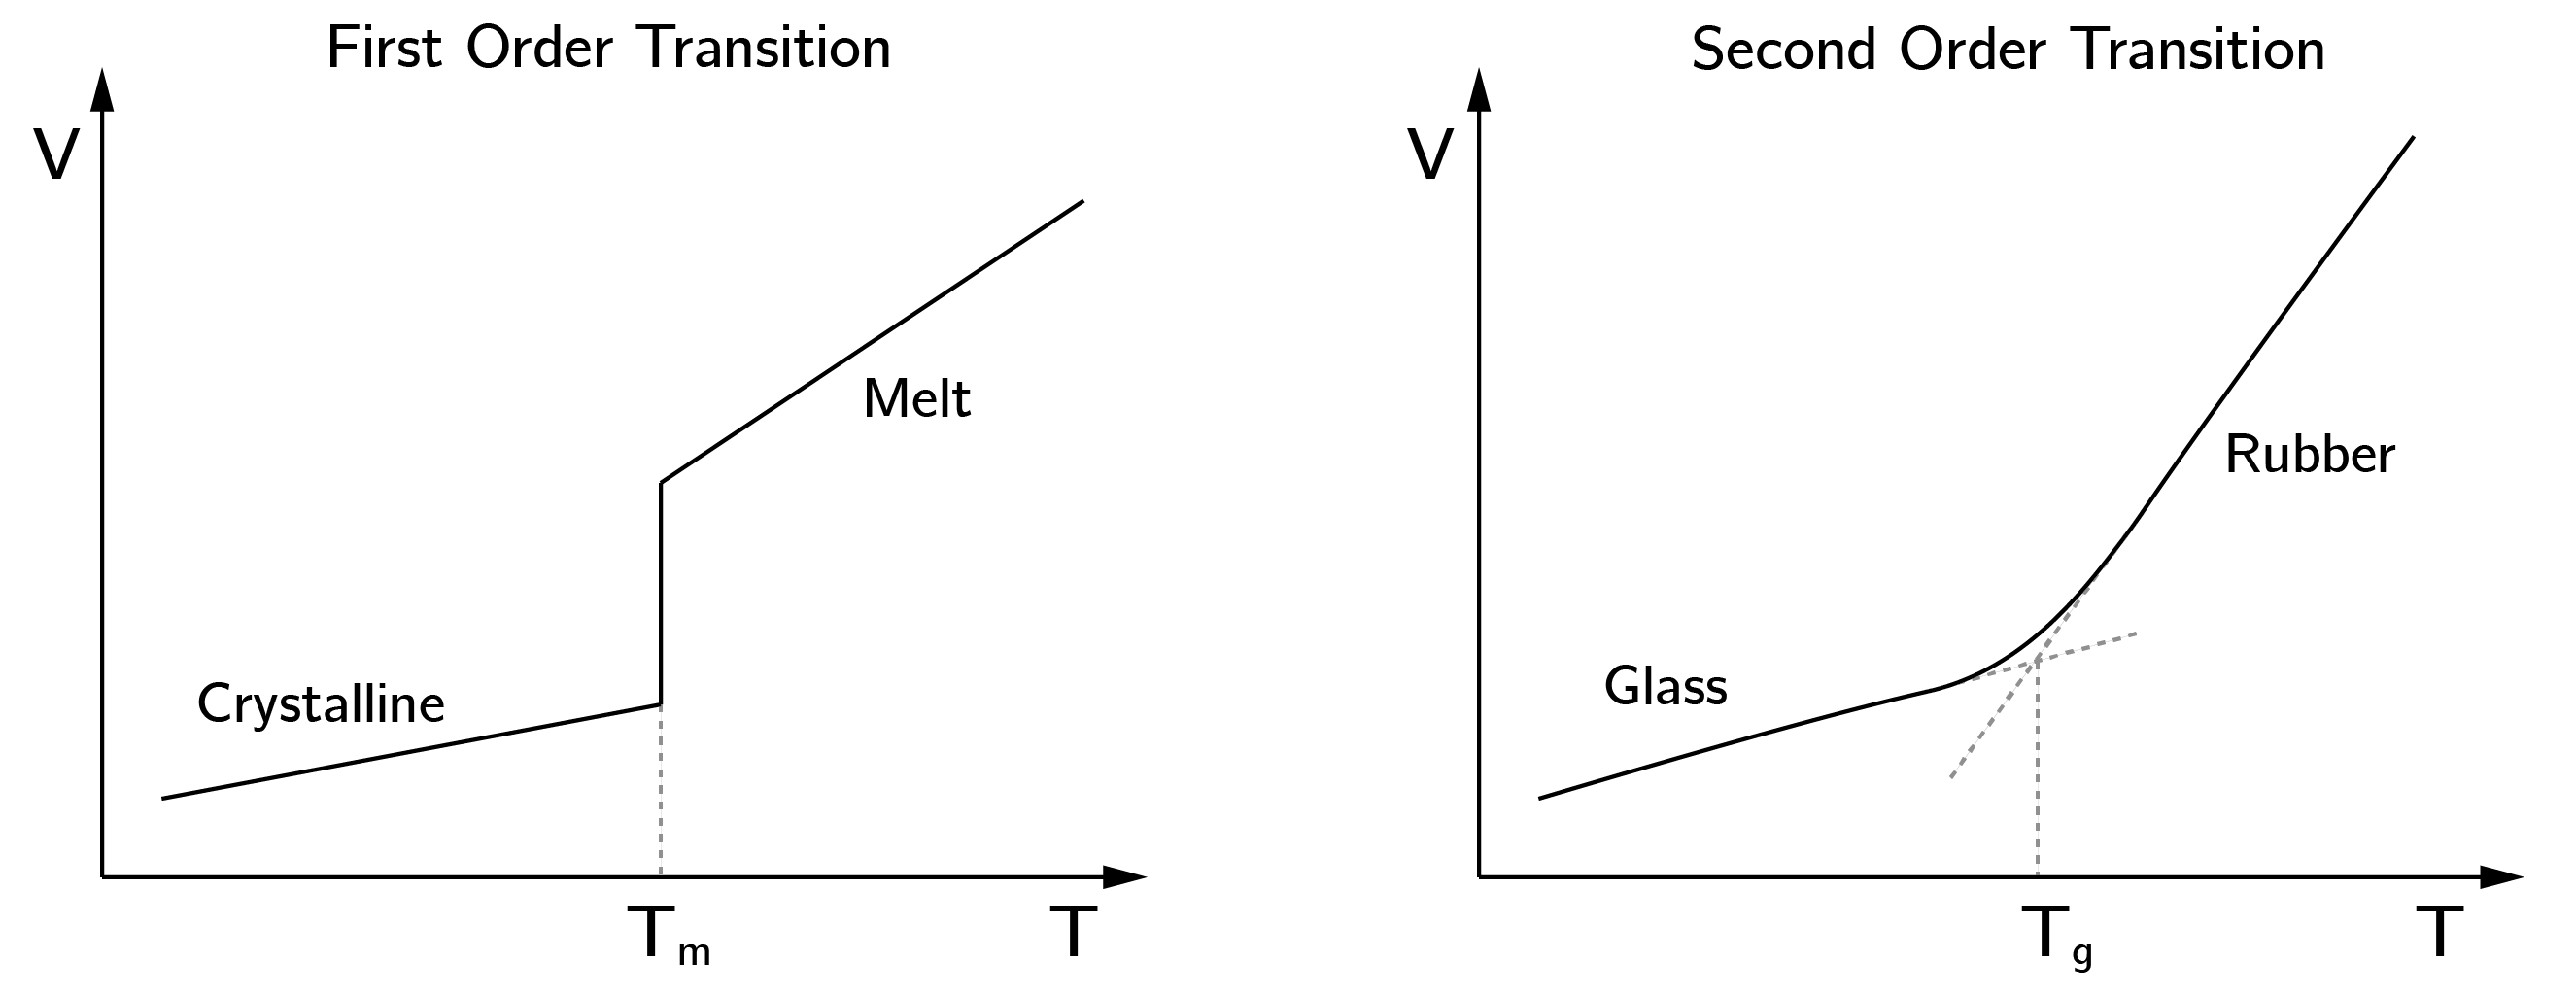
\includegraphics{media/ch3/ch3-1-may31.png}

}

\caption{\label{fig-ch3-img1-old-13}A first-order (discontinuous) and
second-order (continuous) phase transition. (Adapted from
\url{https://polymerdatabase.com/polymer\%20physics/ThemalTransitions.html})}

\end{figure}%

Discontinuous phase transitions such as melting and freezing occur in
many systems. Famous examples from the natural sciences include
collapsing bridges, capsizing ships, cell division, and climate
transitions such as the onset of ice ages. Examples from the social
sciences include conflict, war, and revolution. Some examples from
psychology are falling asleep, outbursts of aggression, radicalization,
falling in love, sudden insights, relapses into depression or addiction,
panic, and multistable perception. The perception of the Necker cube is
a famous example (figure~\ref{fig-ch3-img2-old-14}). Building and
testing models of these psychological transitions is challenging but
rewarding. These transitions involve large changes in behavior, in
contrast to the smaller, often marginally significant effects typically
observed in psychological intervention studies.

\begin{figure}

\centering{

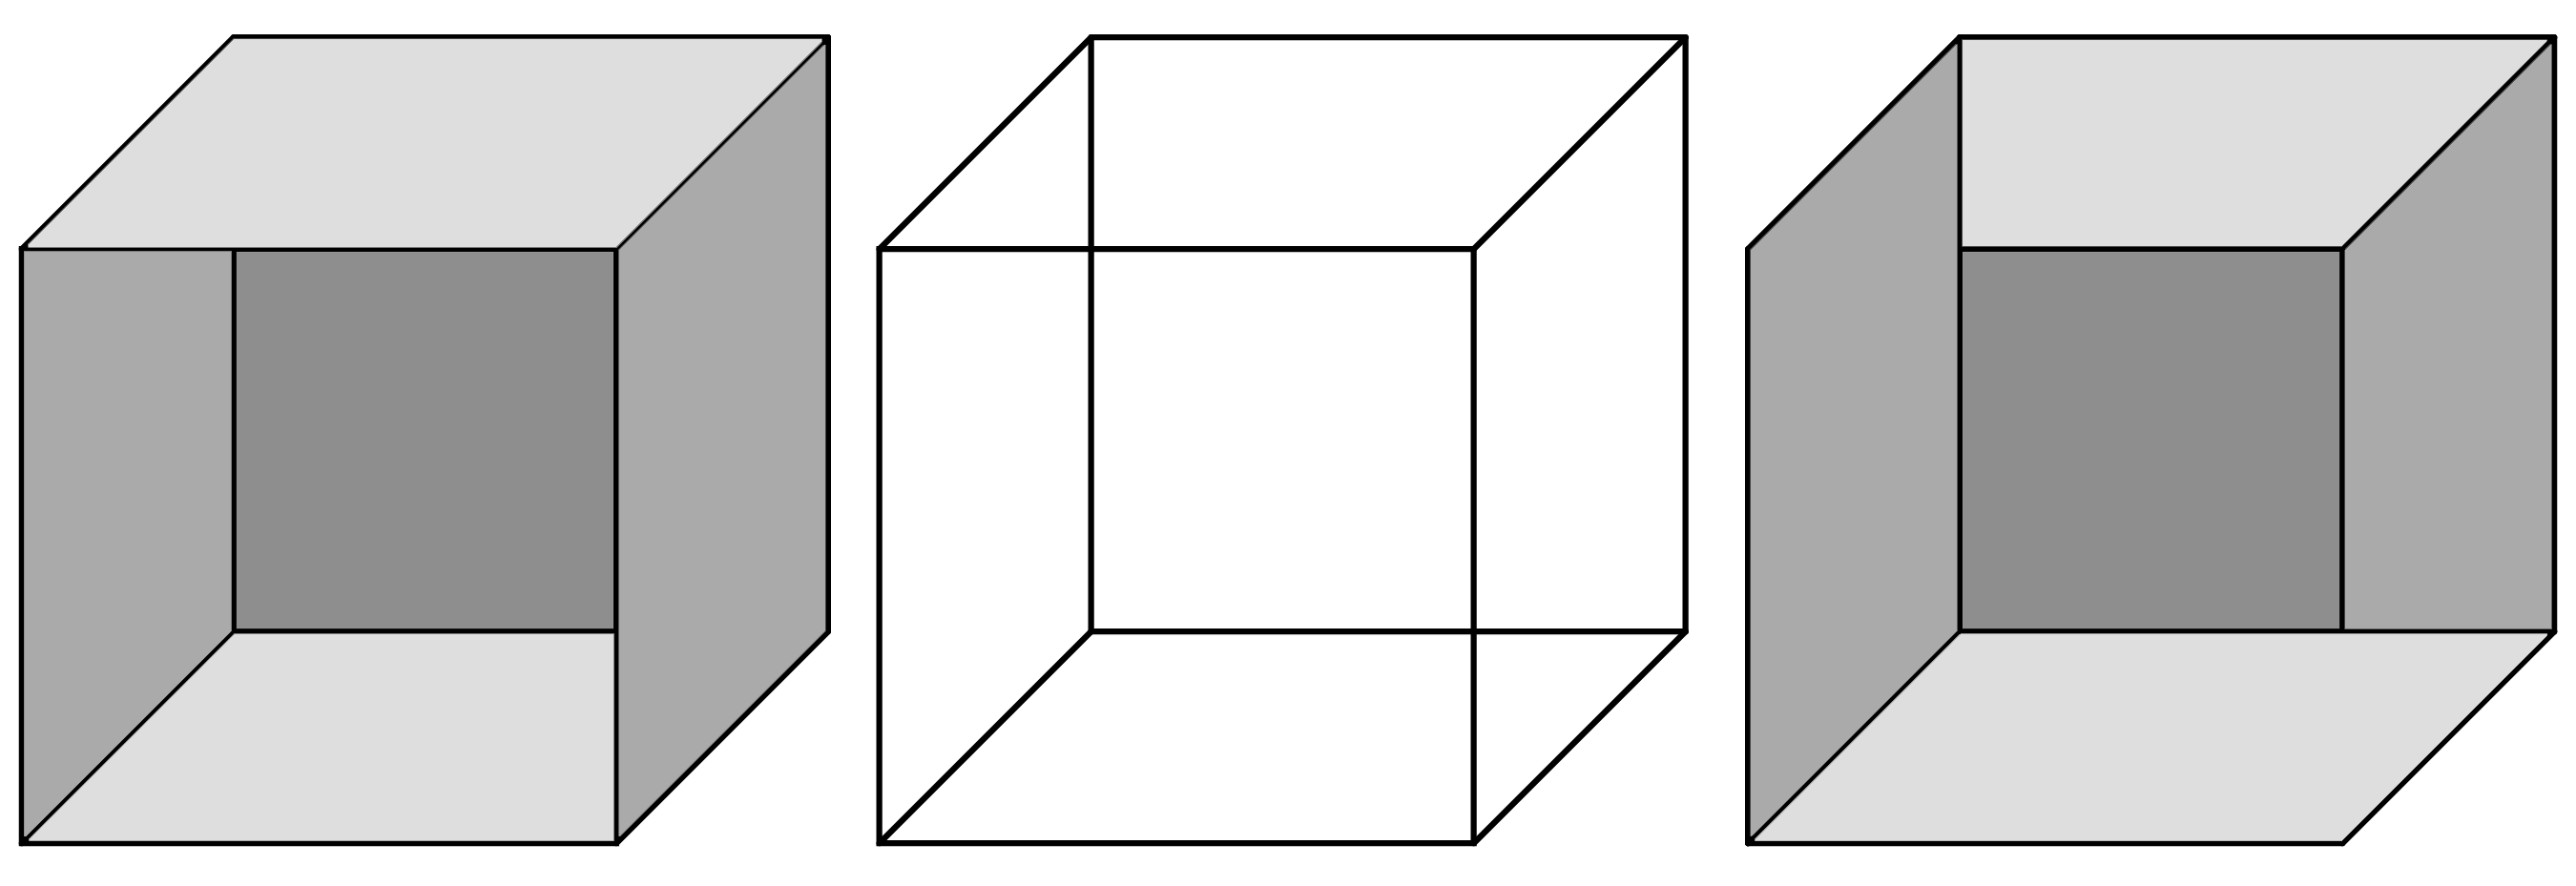
\includegraphics[width=13cm,height=\textheight]{media/ch3/ch3-02__figure14.png}

}

\caption{\label{fig-ch3-img2-old-14}Transitions in the perception of the
Necker cube. The perception of the middle cube is bistable, and sudden
transitions occur between the left (``front'') and right (``back'')
percepts. Multistable perception is a much-studied psychological
phenomenon that is still not fully understood.}

\end{figure}%

\section{Bifurcation and Catastrophe
theory}\label{sec-Bifurcation-and-Catastrophe-theory}

{\marginnote{\begin{footnotesize}Bifurcation theory is a branch of
mathematics that studies changes in the qualitative or topological
structure of a given family of dynamical systems as parameters are
smoothly varied.\end{footnotesize}}} Bifurcations occur when equilibria
disappear, appear, or split. Simply put, bifurcation theory studies how
small changes in parameters or conditions can lead to large changes in
outcomes in mathematical systems.

Catastrophe theory can be viewed as a branch of bifurcation theory,
describing a subclass of bifurcations. It was developed by René Thom
(1977) and popularized by Christopher Zeeman (1976). The reason I chose
to focus on catastrophe theory in this chapter is fourfold: First, it
provides one of the few systematic treatments of bifurcations. A
systematic treatment is more effective than simply listing all types of
bifurcations. Second, once you have a grasp of the basics of catastrophe
theory, it becomes easier to learn about other bifurcations not
encompassed by this theory. Third, it is the most widely used approach
in psychology and the social sciences. Finally, the field has developed
an empirical program and statistical procedures for the practical
application of catastrophe theory.

{\marginnote{\begin{footnotesize}In gradient systems some quantity is
minimized or maximized.\end{footnotesize}}} Catastrophe theory is
concerned with gradient systems. These are dynamic systems that can be
described by a potential function. Potential functions can be thought of
as landscapes with minima and maxima in which we throw a ball and see
where it ends up. The simplest case, discussed in the next section, is
the quadratic minimum. {\marginnote{\begin{footnotesize}A potential
function in mathematics describes the potential energy landscape of a
system, where the system's dynamics are determined by the gradients of
this function.\end{footnotesize}}} We can also study what happens to the
ball if the landscape changes shape smoothly and a minimum disappears.
Then sudden jumps can occur.

Minima and maxima are called critical points, points where the first
derivative of the potential function is 0. Catastrophe theory analyzes
so-called degenerate critical points of the potential function. Phase
transitions can occur at these bifurcation points. Thom proved that
there are only seven fundamental types of catastrophes (given a limited
set of control parameters). I will start with a mathematical
introduction and, after explaining the main concepts, give some
psychological examples. {\marginnote{\begin{footnotesize}Degenerate
critical points are points where not only the first derivative but also
the second derivative of the potential function is
zero.\end{footnotesize}}} An in-depth discussion of the role of
potential functions in catastrophe theory can be found in the
introduction of chapter 1 of Gilmore (1993).

\subsection{The quadratic case}\label{sec-The-quadratic-case}

Thom's theorems are known to be highly complicated, but the basic
concepts are not that difficult to grasp. The simplest potential
function is

\begin{equation}\phantomsection\label{eq-ch3-1-old-5}{
V(X) = X^{2}
}\end{equation}

\begin{figure}

\centering{

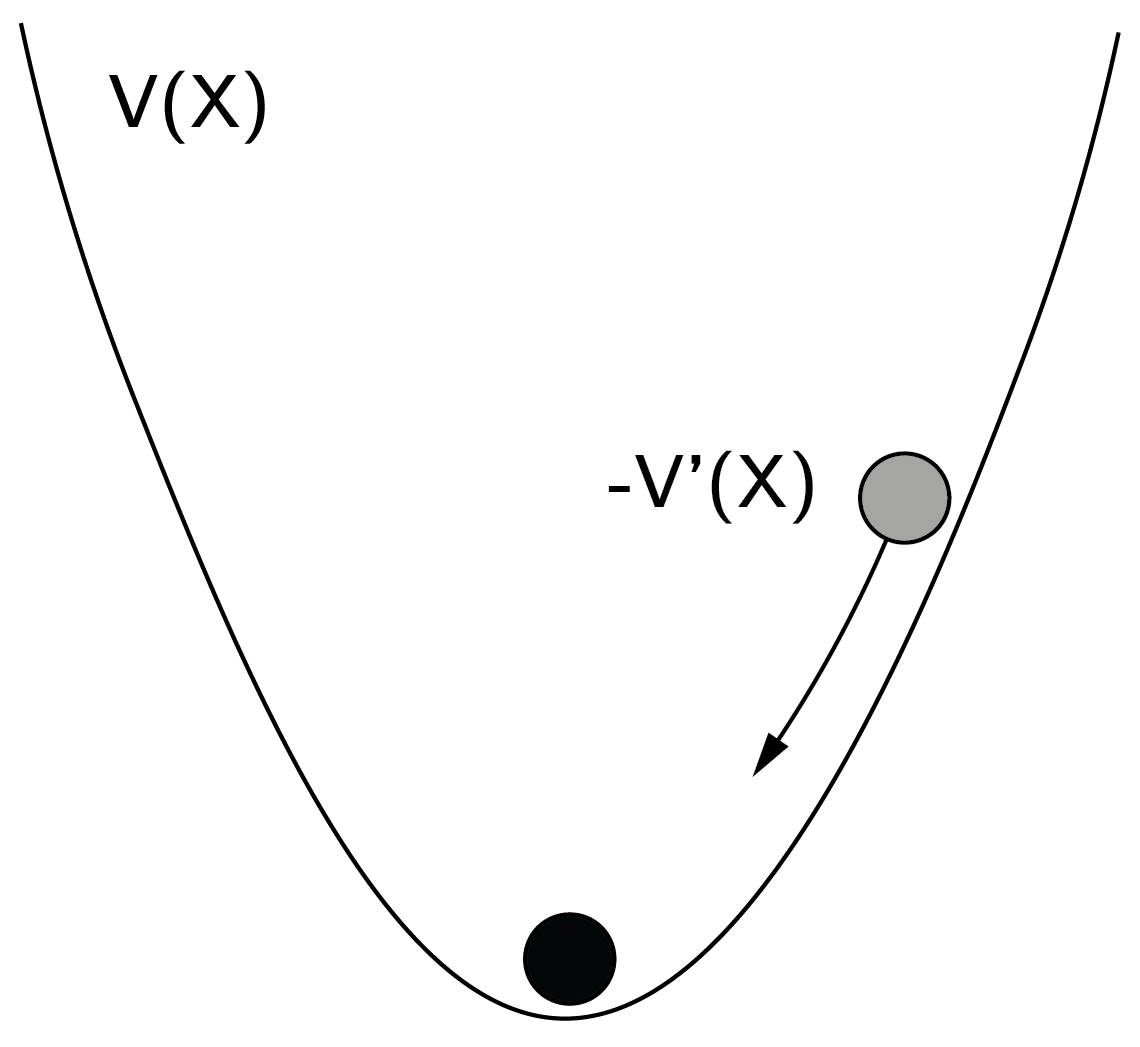
\includegraphics{media/ch3/ch3-3-may31.png}

}

\caption{\label{fig-ch3-img3-old-15}The quadratic potential function. A
ball rolls to the minimum value of \(V(X)\). Its change is defined by
the negative of the derivative of the potential function \(-V'(X)\).}

\end{figure}%

Imagine a ball in a landscape. The ball will roll to the minimum of the
potential function (figure~\ref{fig-ch3-img3-old-15}). We learned in
school that this is the point where the first derivative is 0 and the
second derivative is positive. The first and second derivatives are
\(V^{'}(X) = 2X\) and \(V^{''}(X) = 2\), respectively. At \(X = 0\) we
find the minimum.

The potential function describes a dynamical system defined by

\begin{equation}\phantomsection\label{eq-ch3-2-old-6}{
\frac{dX}{dt} = - V^{'}(X).
}\end{equation}

This makes sense. When the ball is in \((1,1)\), \(- V^{'}(X) = - 2\)
and the ball will move toward \(X = 0\). But if \(X = 0\),
\(- V^{'}(X) = 0\), and the ball will not move anymore. In the case of
the quadratic potential function, there is only one fixed point. By
adding parameters and lower order terms to \(V\), that is,
\({aX + X}^{2}\), we can move its location, but the qualitative form
(one stable fixed point) will not change. Also note that the second
derivative is positive, which tells us that we are dealing with a
minimum and not a maximum (the so-called second derivative test).

Many dynamical systems behave according to this potential
function.\footnote{As we will see in
  section~\ref{sec-Cobbs-maximum-likelihood-approach}, the statistical
  equivalent of the quadratic potential function is the normal
  distribution, the most popular distribution in our statistical work.}
Nothing spectacular happens: no bifurcations and no jumps. This is
different when we consider potential functions with higher order terms.

\subsection{The fold catastrophe}\label{sec-The-fold-catastrophe}

The fold catastrophe is defined by the potential function

\begin{equation}\phantomsection\label{eq-ch3-3-old-7}{
V(X) = {- aX + X}^{3}.
}\end{equation}

This function has a degenerate critical (bifurcation) point at
\(X = 0, a = 0\), because at this point \(V^{'}(X) = - a + 3X^{2} = 0\)
and \(V^{''}(X) = 6X = 0\), so both the first and second derivative are
0. What makes this point so special? This is illustrated in
figure~\ref{fig-ch3-img4-old-16}.

\begin{figure}

\centering{

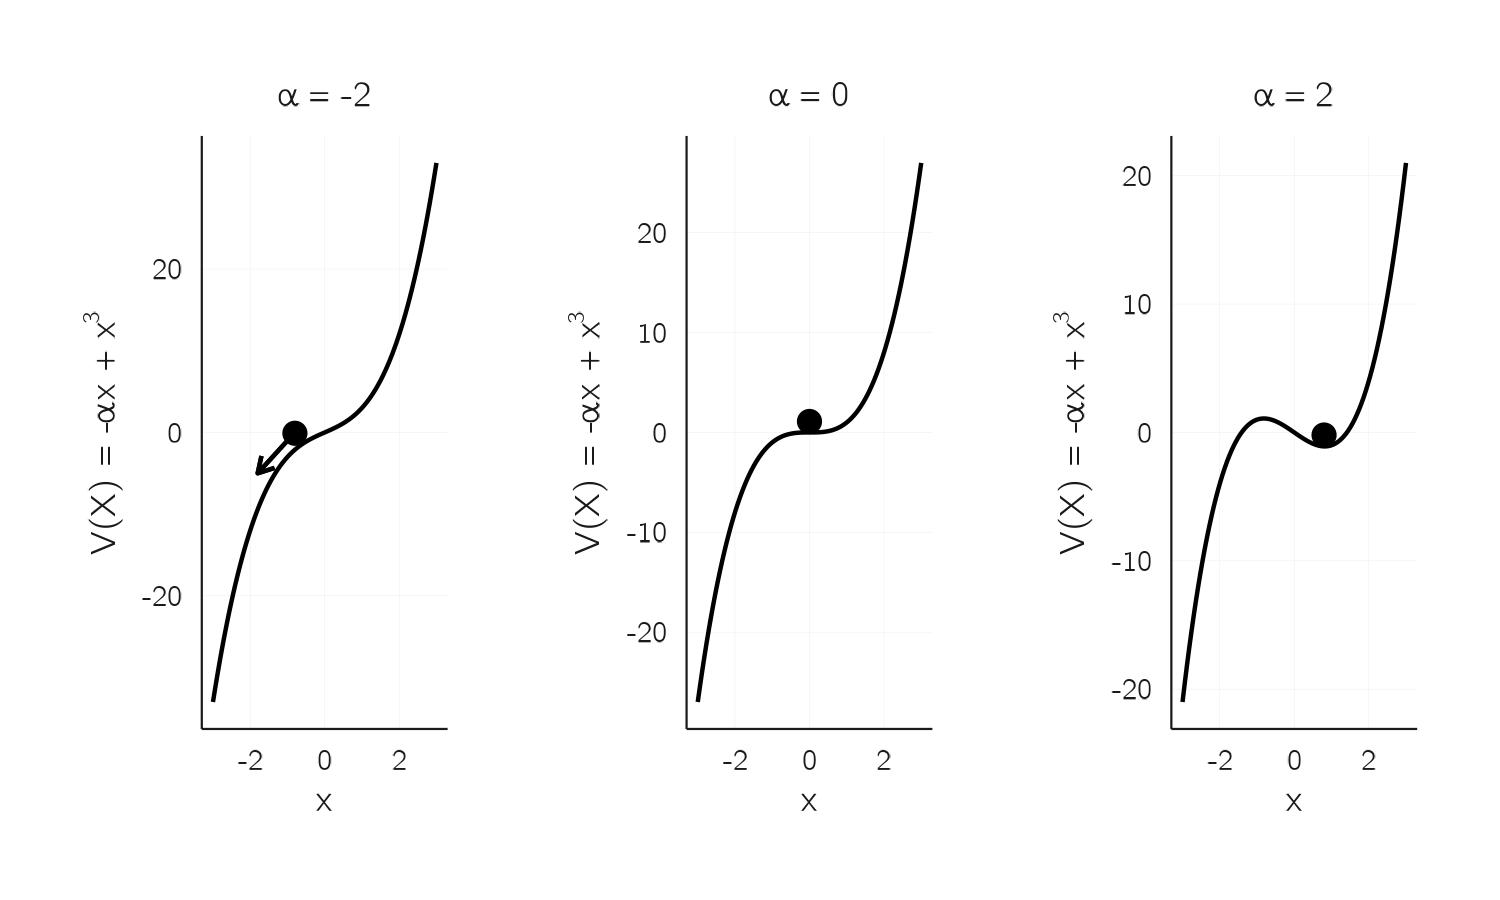
\includegraphics{media/ch3/fig-ch3-img4-old-16.jpg}

}

\caption{\label{fig-ch3-img4-old-16}A bifurcation at \(a = 0\): the
equilibria change qualitatively. For \(a<0\) there is no equilibrium;
for \(a>0\) we have a minimum and a maximum.}

\end{figure}%

\begin{Shaded}
\begin{Highlighting}[]
\FunctionTok{layout}\NormalTok{(}\FunctionTok{t}\NormalTok{(}\DecValTok{1}\SpecialCharTok{:}\DecValTok{3}\NormalTok{))}
\NormalTok{v }\OtherTok{\textless{}{-}} \ControlFlowTok{function}\NormalTok{(x,a) }\SpecialCharTok{{-}}\NormalTok{a }\SpecialCharTok{*}\NormalTok{ x }\SpecialCharTok{+}\NormalTok{ x}\SpecialCharTok{\^{}}\DecValTok{3} 
\FunctionTok{curve}\NormalTok{(}\FunctionTok{v}\NormalTok{(x,}\AttributeTok{a=}\SpecialCharTok{{-}}\DecValTok{2}\NormalTok{),}\SpecialCharTok{{-}}\DecValTok{3}\NormalTok{,}\DecValTok{3}\NormalTok{,}\AttributeTok{bty=}\StringTok{\textquotesingle{}n\textquotesingle{}}\NormalTok{)}
\FunctionTok{curve}\NormalTok{(}\FunctionTok{v}\NormalTok{(x,}\AttributeTok{a=}\DecValTok{0}\NormalTok{),}\SpecialCharTok{{-}}\DecValTok{3}\NormalTok{,}\DecValTok{3}\NormalTok{,}\AttributeTok{bty=}\StringTok{\textquotesingle{}n\textquotesingle{}}\NormalTok{)}
\FunctionTok{curve}\NormalTok{(}\FunctionTok{v}\NormalTok{(x,}\AttributeTok{a=}\DecValTok{2}\NormalTok{),}\SpecialCharTok{{-}}\DecValTok{3}\NormalTok{,}\DecValTok{3}\NormalTok{,}\AttributeTok{bty=}\StringTok{\textquotesingle{}n\textquotesingle{}}\NormalTok{)}
\end{Highlighting}
\end{Shaded}

In the left plot, \(a < 0\) and there is no fixed point; the ball rolls
away to minus infinity. This can be checked by setting the first
derivative to zero, which gives \(X = \pm \sqrt{{a}/{3}}\). For negative
\(a\) there is no solution. A positive value of \(a\) gives two
solutions, as shown on the right for \(a = 2\). The positive solution
\(X = \sqrt{2/3}\) is a stable fixed point because the second derivative
in this point is positive. The negative solution \(X = - \sqrt{2/3}\) is
an unstable fixed point because the second derivative in this point is
negative.

The middle figure depicts the case just in between these two cases. Here
the equilibrium is an inflection point, a degenerate critical point. The
bifurcation occurs at this point as we go from a landscape with no fixed
points to one with two, one stable and one unstable.

Another way to visualize this is by making a bifurcation diagram as we
did for the logistic map in Chapter~\ref{sec-ch2}. On the x-axis we put
\(a\), from \(-1\) to \(2\). On the y-axis we plot \(X^{*}\), the fixed
points of equation~\ref{eq-ch3-3-old-7}. We use lines for stable fixed
points and dashed lines for unstable points. The diagram is shown in
figure~\ref{fig-ch3-img5-old-17}. {\marginnote{\begin{footnotesize}Note
that the fold is not accompanied by sudden jumps in behavior. It is an
example of a second-order phase transition.\end{footnotesize}}}

\begin{figure}

\centering{

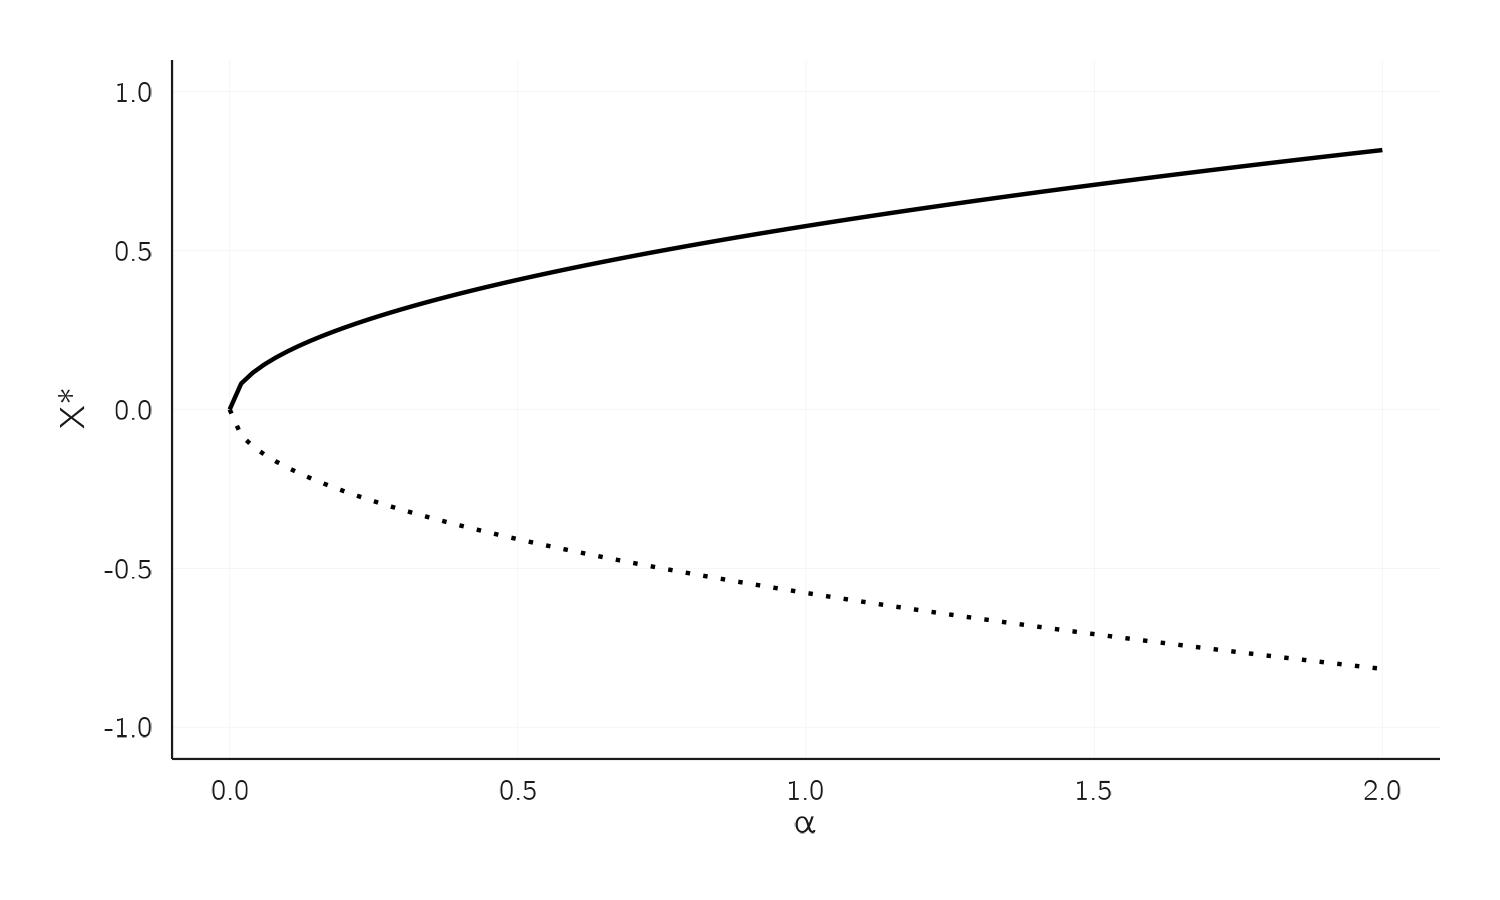
\includegraphics[width=10cm,height=\textheight]{media/ch3/fig-ch3-img5-old-17.jpg}

}

\caption{\label{fig-ch3-img5-old-17}The bifurcation diagram of the fold
catastrophe. Similar to what's shown in figure~\ref{fig-ch3-img4-old-16}
, when \(a=0\), there is a dramatic change in the equilibrium landscape.
Suddenly, both a stable and an unstable equilibrium emerge, seemingly
from nowhere.}

\end{figure}%

This bifurcation diagram may not look as spectacular as the logistic
map, but its importance cannot be overstated. The fold is everywhere! In
a fascinating book, \emph{The Seduction of Curves}, Allen McRobie (2017)
shows that whenever we see an edge, we see a fold.
Figure~\ref{fig-ch3-img6-old-18} is from the book, where he demonstrates
how different catastrophes appear in art. I also recommend his YouTube
lecture.\footnote{\url{https://www.youtube.com/watch?v=6ZQKzcw9Ulk}}

\begin{figure}

\centering{

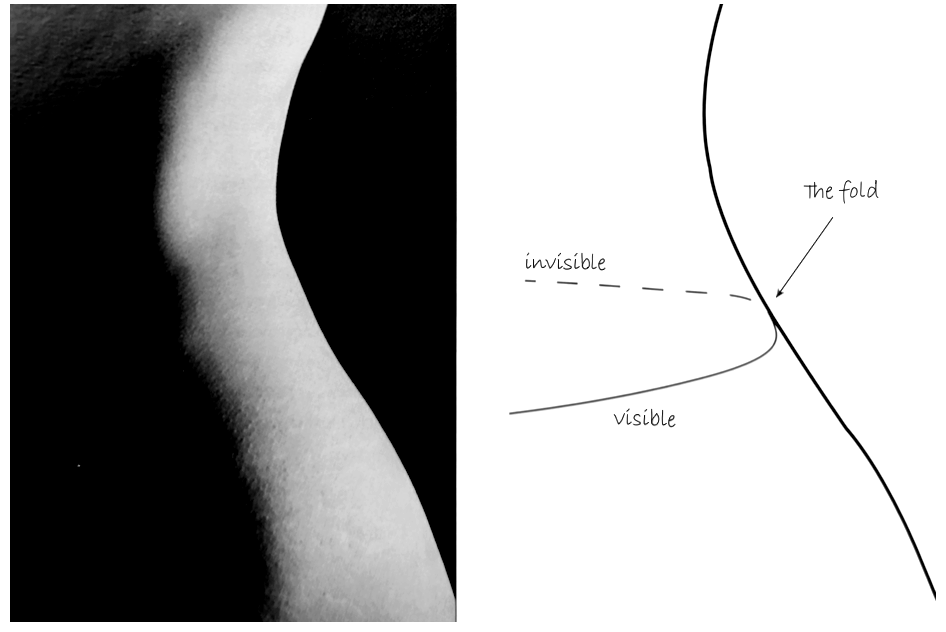
\includegraphics{media/ch3/ch3-6__figure18.png}

}

\caption{\label{fig-ch3-img6-old-18}The fold in drawings (from McRobie
2017). The fold line separates the parts that can be seen from the parts
that are hidden.}

\end{figure}%

The fold catastrophe has been studied in fields from evolution theory
(Dodson and Hallam 1977) to buoyancy in diving (Güémez, Fiolhais, and
Fiolhais 2002). In addition, higher-order catastrophes are composed of
folds. {\marginnote{\begin{footnotesize}The fold catastrophe is also
known as a saddle node, tangential, or blue-sky
bifurcation.\end{footnotesize}}}

\subsection{The cusp catastrophe}\label{sec-The-cusp-catastrophe}

{\marginnote{\begin{footnotesize}Sudden jumps between stable states are
associated with first order phase transitions.\end{footnotesize}}} The
cusp, the best-known catastrophe, is the simplest catastrophe showing
sudden jumps in behavior. The potential function of the cusp is

\begin{equation}\phantomsection\label{eq-ch3-4-old-8}{ V(X) = - aX - \frac{1}{2}bX^{2} + \frac{1}{4}X^{4}. }\end{equation}

The half and quarter are added to make later derivations a little
easier. The highest power is now 4. The first two terms contain the
control variables \(a\) and \(b\), known as the normal and splitting
variables. {\marginnote{\begin{footnotesize}Control variables are the
parameters whose gradual changes induce qualitative change in the
behavior of the system.\end{footnotesize}}} You might ask why there is
no third order term. The nontechnical answer is that such a term would
not change the qualitative behavior of the bifurcation. Catastrophe
theory studies bifurcations that are structurally stable, meaning that
perturbing the equations (and not just the parameters) does not
fundamentally change the behavior (see
section~\ref{sec-Other-bifurcations} and Stewart (1982) for further
explication).

I advise you to do some minimal research on this equation yourself,
using an online graphic calculator tool like Desmos or GeoGebra (paste
f(X)=-a X-(1/2) b X\^{}2+(1/4) X\^{}4). For example, set \(a = 1\) and
\(b = 3\) and look at the graph of the potential function. Think in
terms of the ball moving to a stable fixed point. What you should see is
that there are three fixed points, of which the middle one is unstable.
This bistability is important. Again, there is a relationship to
unpredictability. Although you know the potential function and the
values of \(a\) and \(b\), you are still not sure where the ball is. It
could be in either of the minima.

Other typical behavior occurs when we slowly vary \(a\ (\)up and down
from -2 to 2), for a positive \(b\) value (\(b = 2).\) This is shown in
figure~\ref{fig-ch3-img7-old-19}. At about \(a = 1.5\) we see the sudden
jump. The left fixed point loses its stability and the ball rolls to the
other minimum.

\begin{figure}

\centering{

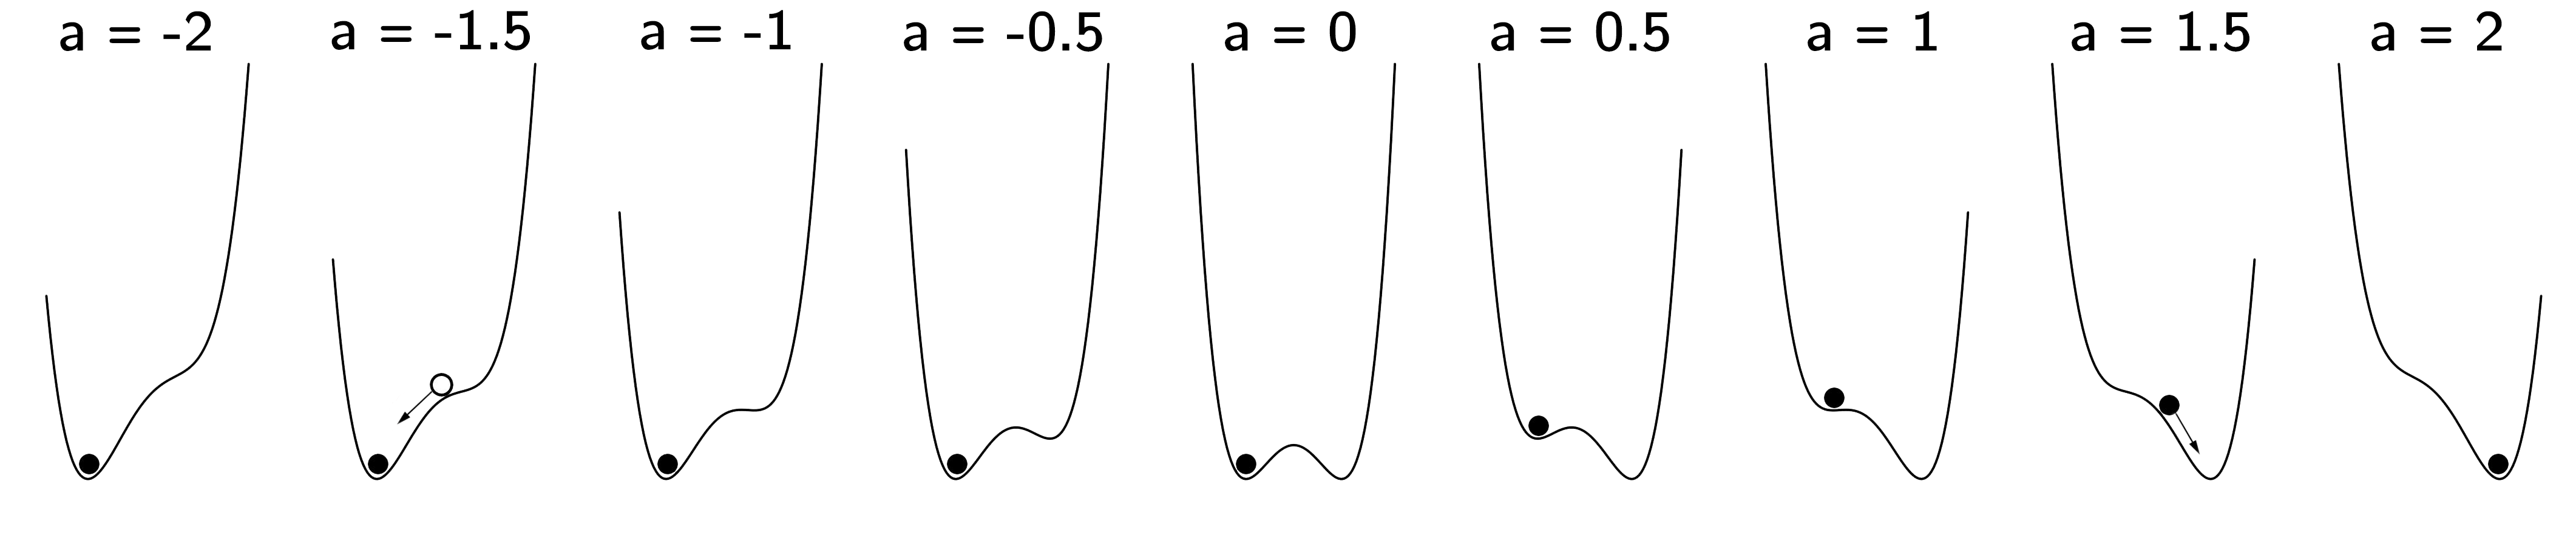
\includegraphics{media/ch3/ch3-7__figure19.png}

}

\caption{\label{fig-ch3-img7-old-19}The change in the potential function
of the cusp by varying \(a\). Note that the jump to the other state does
not happen at \(a=0\) but is delayed and depends on the direction of the
change in \(a\). This delay is called hysteresis.}

\end{figure}%

Now consider what will happen if we decrease \(a\) from 2 to -2.
{\marginnote{\begin{footnotesize}Hysteresis means lagging behind, or
resistance to change.\end{footnotesize}}}. In this case, the ball will
stay in the right minimum until \(a = - 1.5\). Where the jump takes
place depends on the direction of the change in \(a\), the normal
variable. The delay in jumps is called hysteresis. Hysteresis is of
great importance in understanding change or lack of change in complex
systems. The state in which the ball is the less deep minimum (for
\(a = 0.5\) in figure~\ref{fig-ch3-img7-old-19}) is often called a
metastable or locally stable state.
{\marginnote{\begin{footnotesize}Metastable states appear to be stable
for some time but are not in their globally stable
state.\end{footnotesize}}}

In his classic paper on the psychophysical law, Stevens (1957) reports
hysteresis in perceptual judgments when properties such as brightness
and loudness are systematically varied from low to high and vice versa.
In this paper he says: ``I'm trying to describe it, not explain it. I am
not sure I know how to explain it.'' To me the cusp at least partially
explains why hysteresis occurs.

Gilmore (1993) made an important point about noise in the system. If
there is a lot of noise, the jumps occur earlier and we see less or no
hysteresis effect. This is called the Maxwell convention as opposed to
the ``delay'' convention. Demonstrating hysteresis therefore requires
precise experimental control.

Another very interesting pattern occurs when \(a = 0\) and \(b\) is
increased (figure~\ref{fig-ch3-img8-old-20}).

\begin{figure}

\centering{

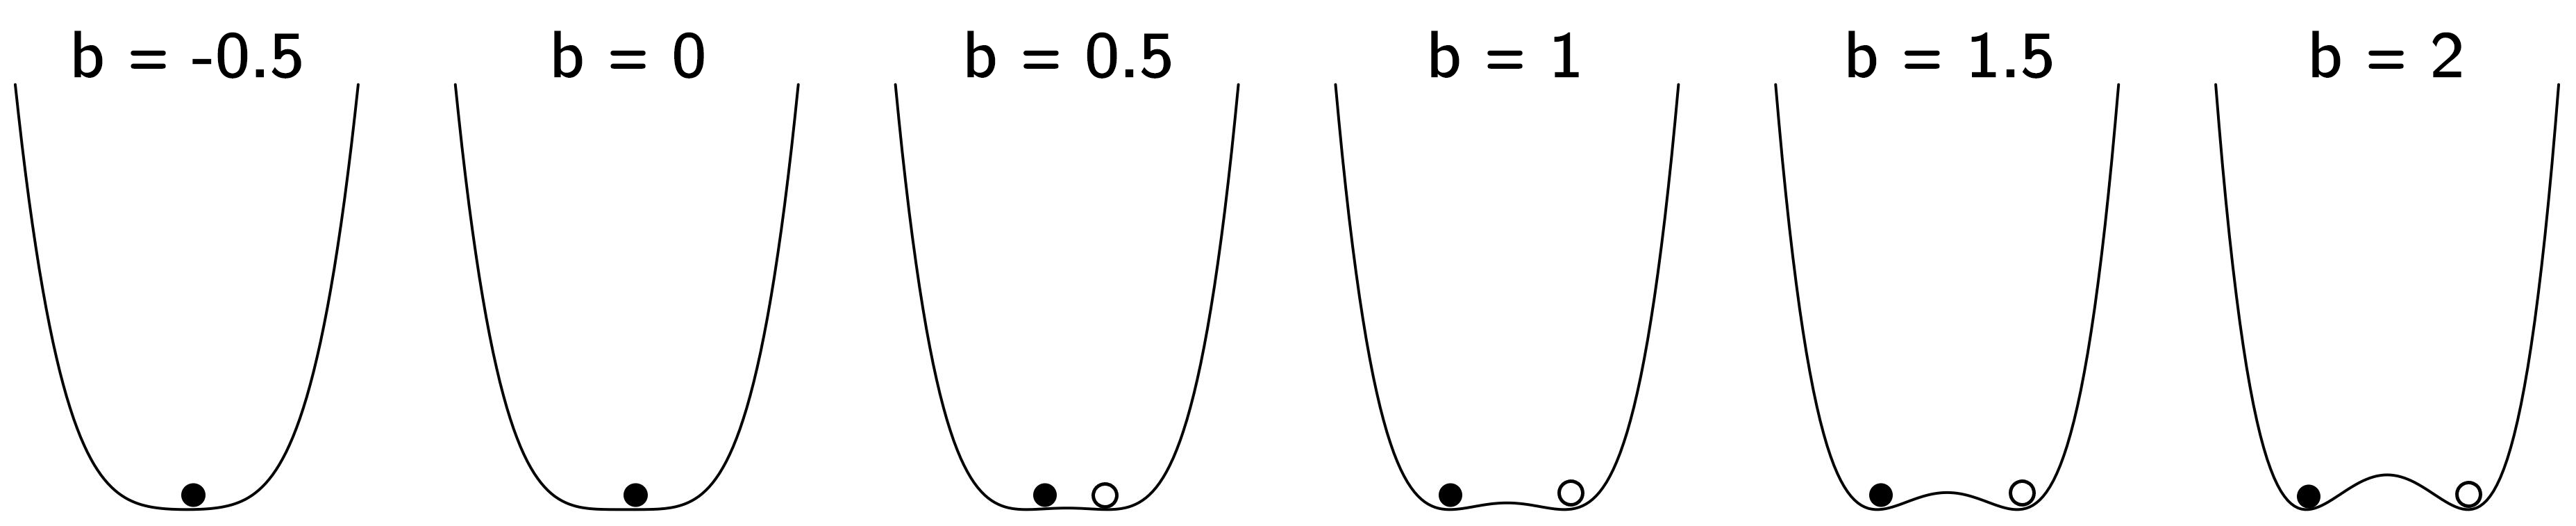
\includegraphics{media/ch3/ch3-8__figure20.png}

}

\caption{\label{fig-ch3-img8-old-20}The change in the potential function
of the cusp by varying \(b\). One minimum splits up in two.}

\end{figure}%

For low \(b\) there is one stable fixed point that becomes unstable. It
splits up into two new stable attractors.
{\marginnote{\begin{footnotesize}A pitchfork bifurcation occurs when a
single equilibrium splits into three (two stable and one unstable) as a
parameter changes, resembling a pitchfork's shape.\end{footnotesize}}}
As we did for the fold, we can make bifurcation diagrams showing the
equilibria of \(X\) as a function of \(a\) and \(b\). Along the
\(a\)-axis we see hysteresis and along the \(b\)-axis we see divergence
or what is often called a pitchfork bifurcation
(figure~\ref{fig-ch3-img9-old-21}).

\begin{figure}

\centering{

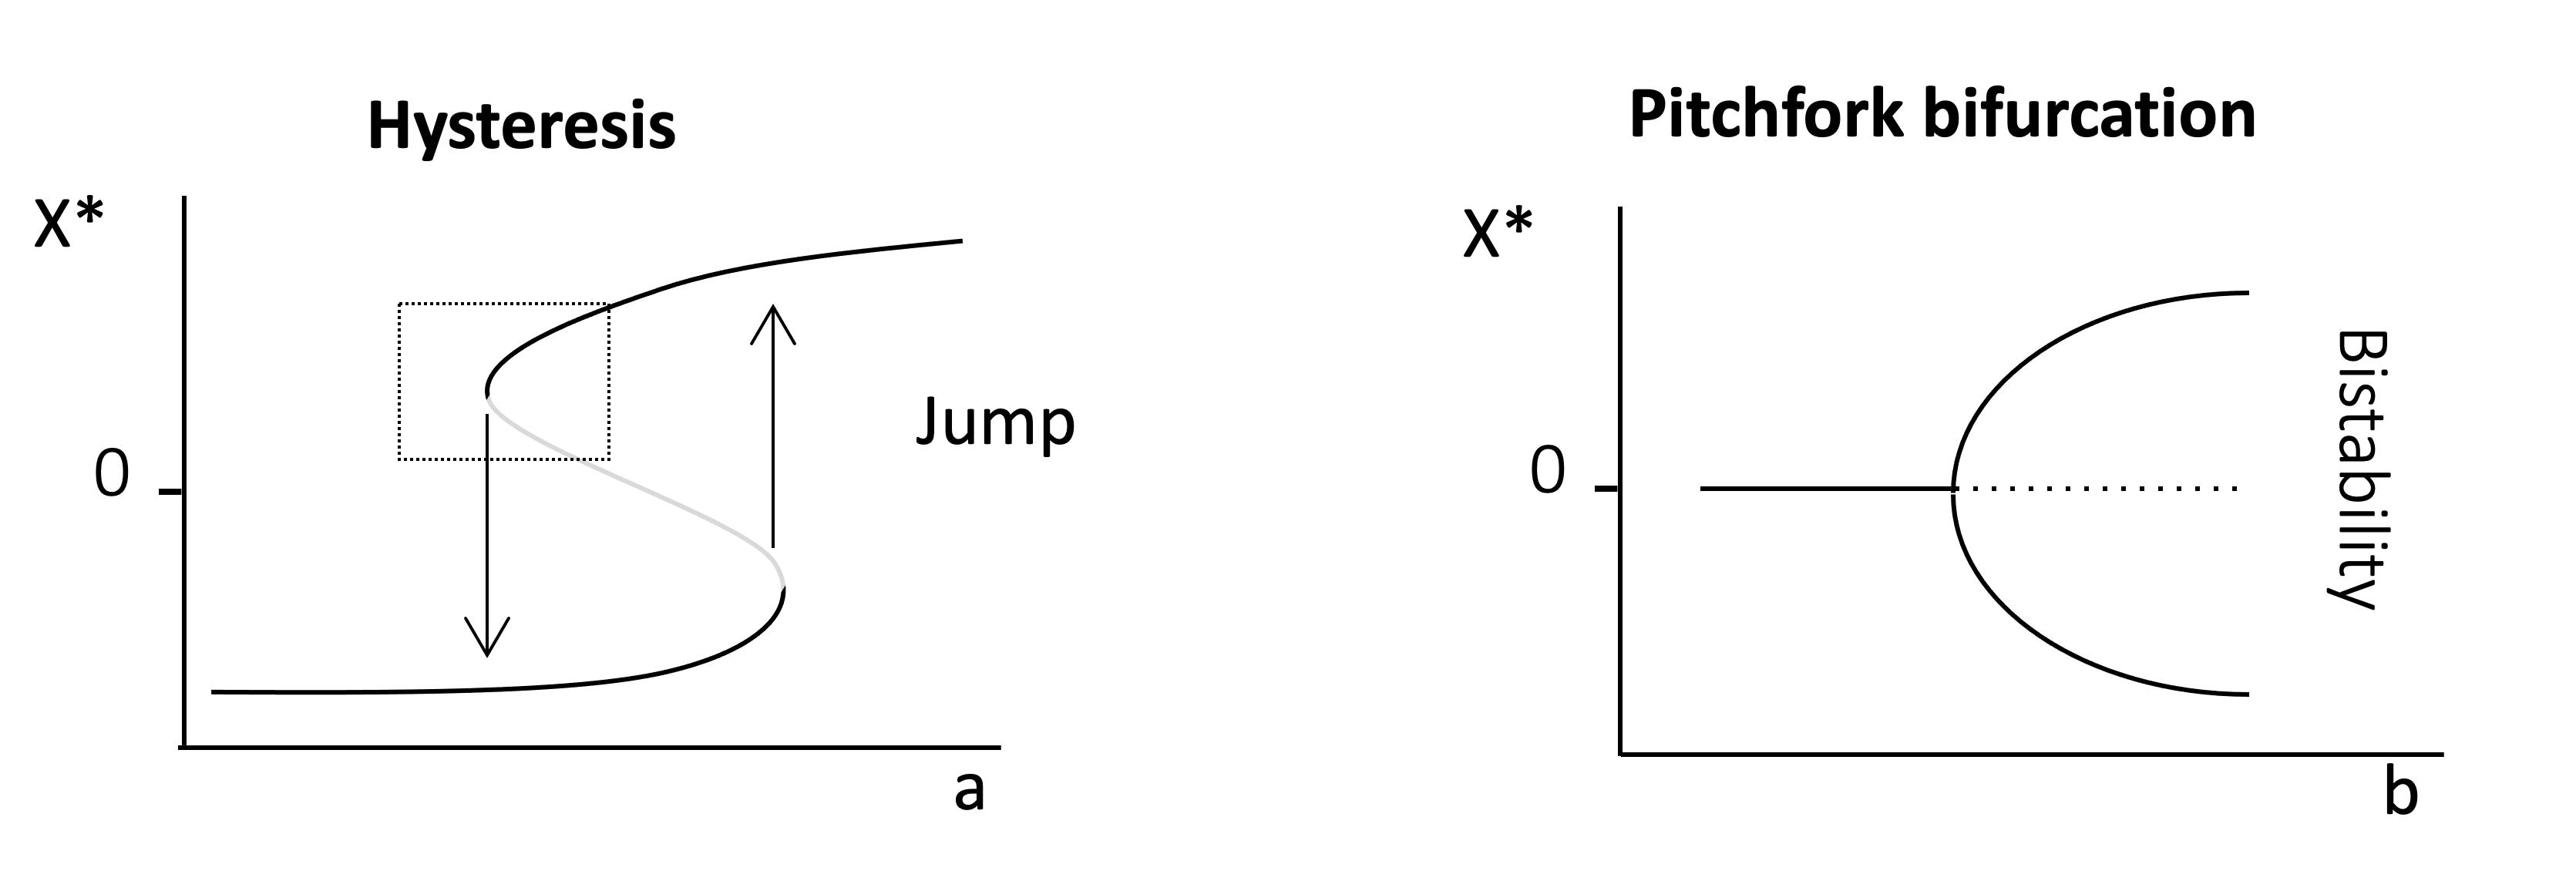
\includegraphics{media/ch3/image9.jpg}

}

\caption{\label{fig-ch3-img9-old-21}Bifurcation plots for the \(a\) and
\(b\) parameters of the cusp. Moving along the \(a\)-axis, assuming
\(b\) is positive, gives hysteresis. Moving along the \(b\) axis,
assuming \(a=0\), gives the pitchfork bifurcation or divergence. The
dotted lines represent unstable maxima. The area in the dotted box in
the first plot is a fold.}

\end{figure}%

Depicting the combined effects of \(a\) and \(b\) requires a
three-dimensional plot, which combines the hysteresis and pitchfork
diagrams (figure~\ref{fig-ch3-img10-old-22}).

\begin{figure}

\centering{

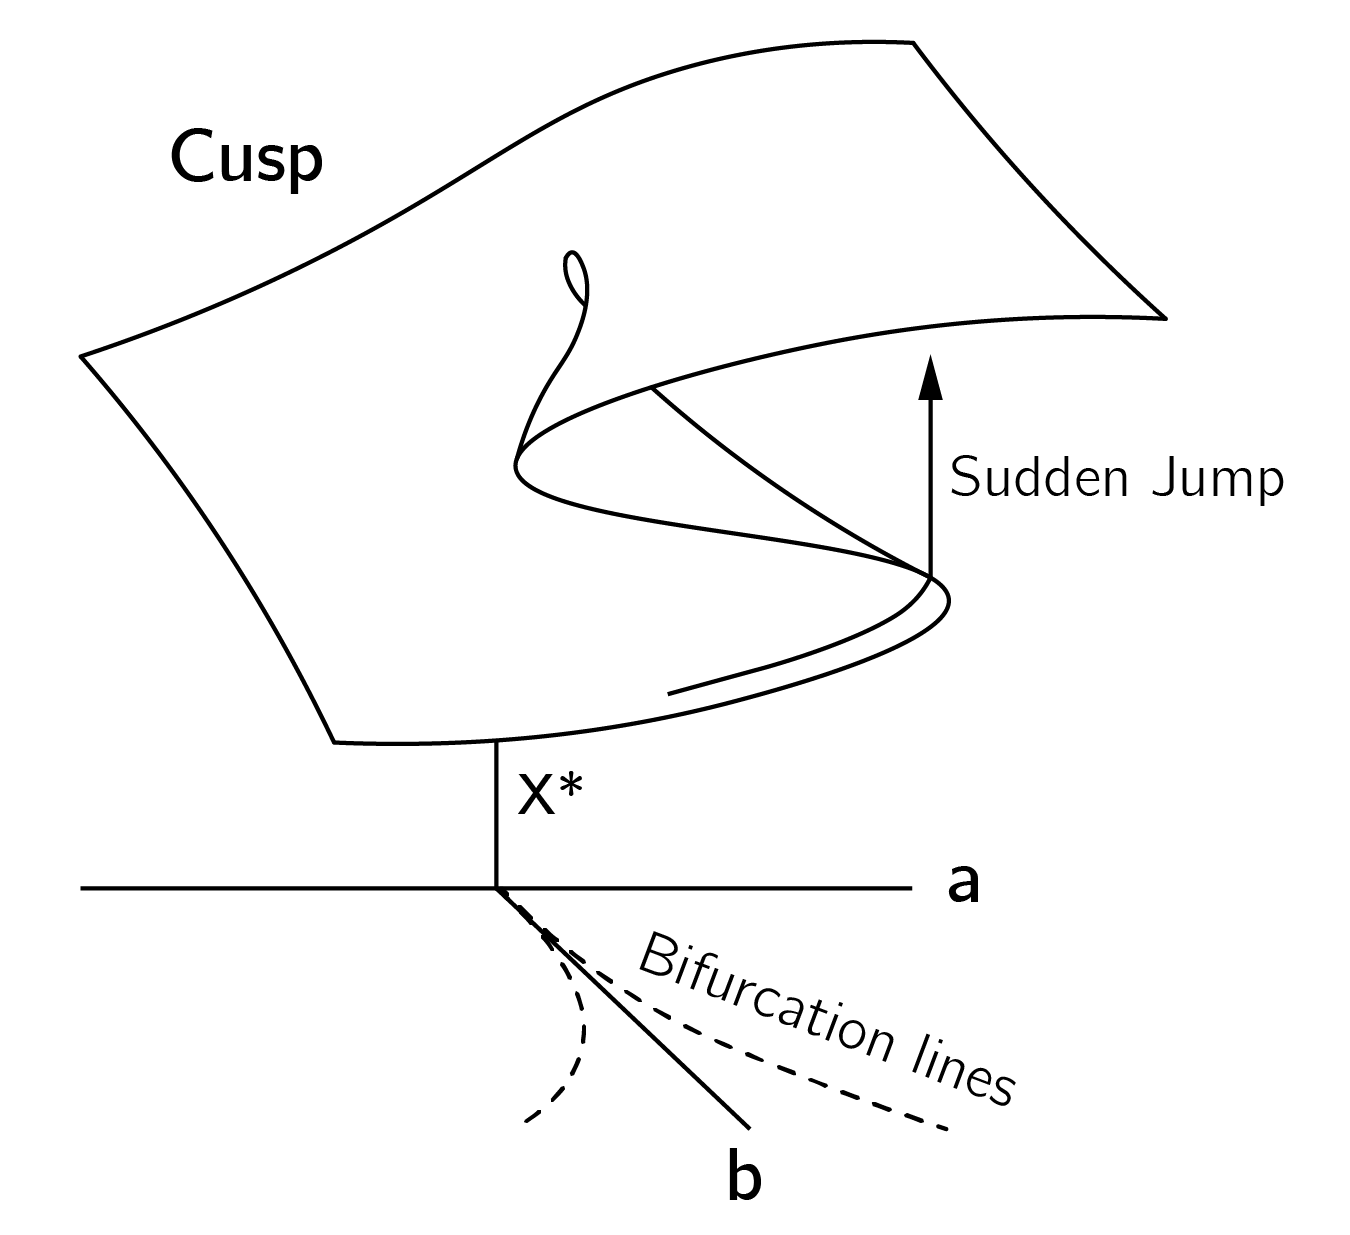
\includegraphics{media/ch3/ch3-10__figure22.png}

}

\caption{\label{fig-ch3-img10-old-22}The cusp catastrophe combines
hysteresis along the normal axis (\(a\)) and the pitchfork along the
splitting axis (\(b\)). At the back of the cusp, changes in \(a\) only
lead to smooth changes in the equilibrium behavior \(X^{*}\). At the
front, sudden jumps occur when we cross the bifurcation lines. These
jumps are typical of first order phase transitions. The area between the
bifurcation lines is called the bifurcation set. In this area there are
two stable and one unstable equilibrium (shaded gray).}

\end{figure}%

The cusp diagram can be expressed mathematically by setting the first
derivative to 0:

\begin{equation}\phantomsection\label{eq-ch3-5-old-9}{
V^{'}(X) = {- a - bX + X}^{3} = 0.
}\end{equation}

This type of equation is called a cubic equation.\footnote{The cubic
  equation cannot be solved easily. This is due to the fact that the
  cusp is not a function of the form \(y = f(x)\). Functions assign to
  each element of \(x\) exactly one element of \(y\). But in bistable
  systems we assign two values of \(y\) to one value of \(x\).} The
degenerate critical points of the cusp can be found by setting the first
and second derivative to 0. This is just within reach of your high
school mathematics training, and I leave this as an exercise. The result
is:

\begin{equation}\phantomsection\label{eq-ch3-6-old-10}{
27a^{2} = 4b^{3}.
}\end{equation}

This equation defines the bifurcation lines where the first and second
derivatives are both 0 and sudden jumps occur (see
figure~\ref{fig-ch3-img10-old-22}). The region between the bifurcation
lines is the bifurcation set. In this region, the bifurcation has three
fixed points, the middle of which is unstable. These unstable states in
the middle are called the inaccessible area, shaded gray in the cusp
diagram. The bifurcation lines meet at (0,0,0). At this point, the third
derivative is also 0. This is the cusp point.

\subsection{Examples of cusp models}\label{sec-Examples-of-cusp-models}

To illustrate the cusp, I always use the business card
(figure~\ref{fig-ch3-img11-old-23}). I recommend that you test this
example (not with your credit card). You can play with two forces.
\(Fv\) is the vertical force and the splitting control variable (\(b\))
in the cusp. \(Fh\) is the horizontal force and the normal variable
(\(a\)) in the cusp. Note that you will only get smooth changes when
\(Fv = 0\), but sudden jumps and hysteresis when you employ vertical
force. One very important phenomenon is that the card has no ``memory''
when \(Fv = 0\). You can push the card to a position, but as soon as you
release this force (\(Fh\) back to 0), the card moves back to the center
position. This is not the case with vertical pressure. If we force the
card to the left or right position, it will stay there, even if we
remove the horizontal force. The card has a memory.

\begin{figure}

\centering{

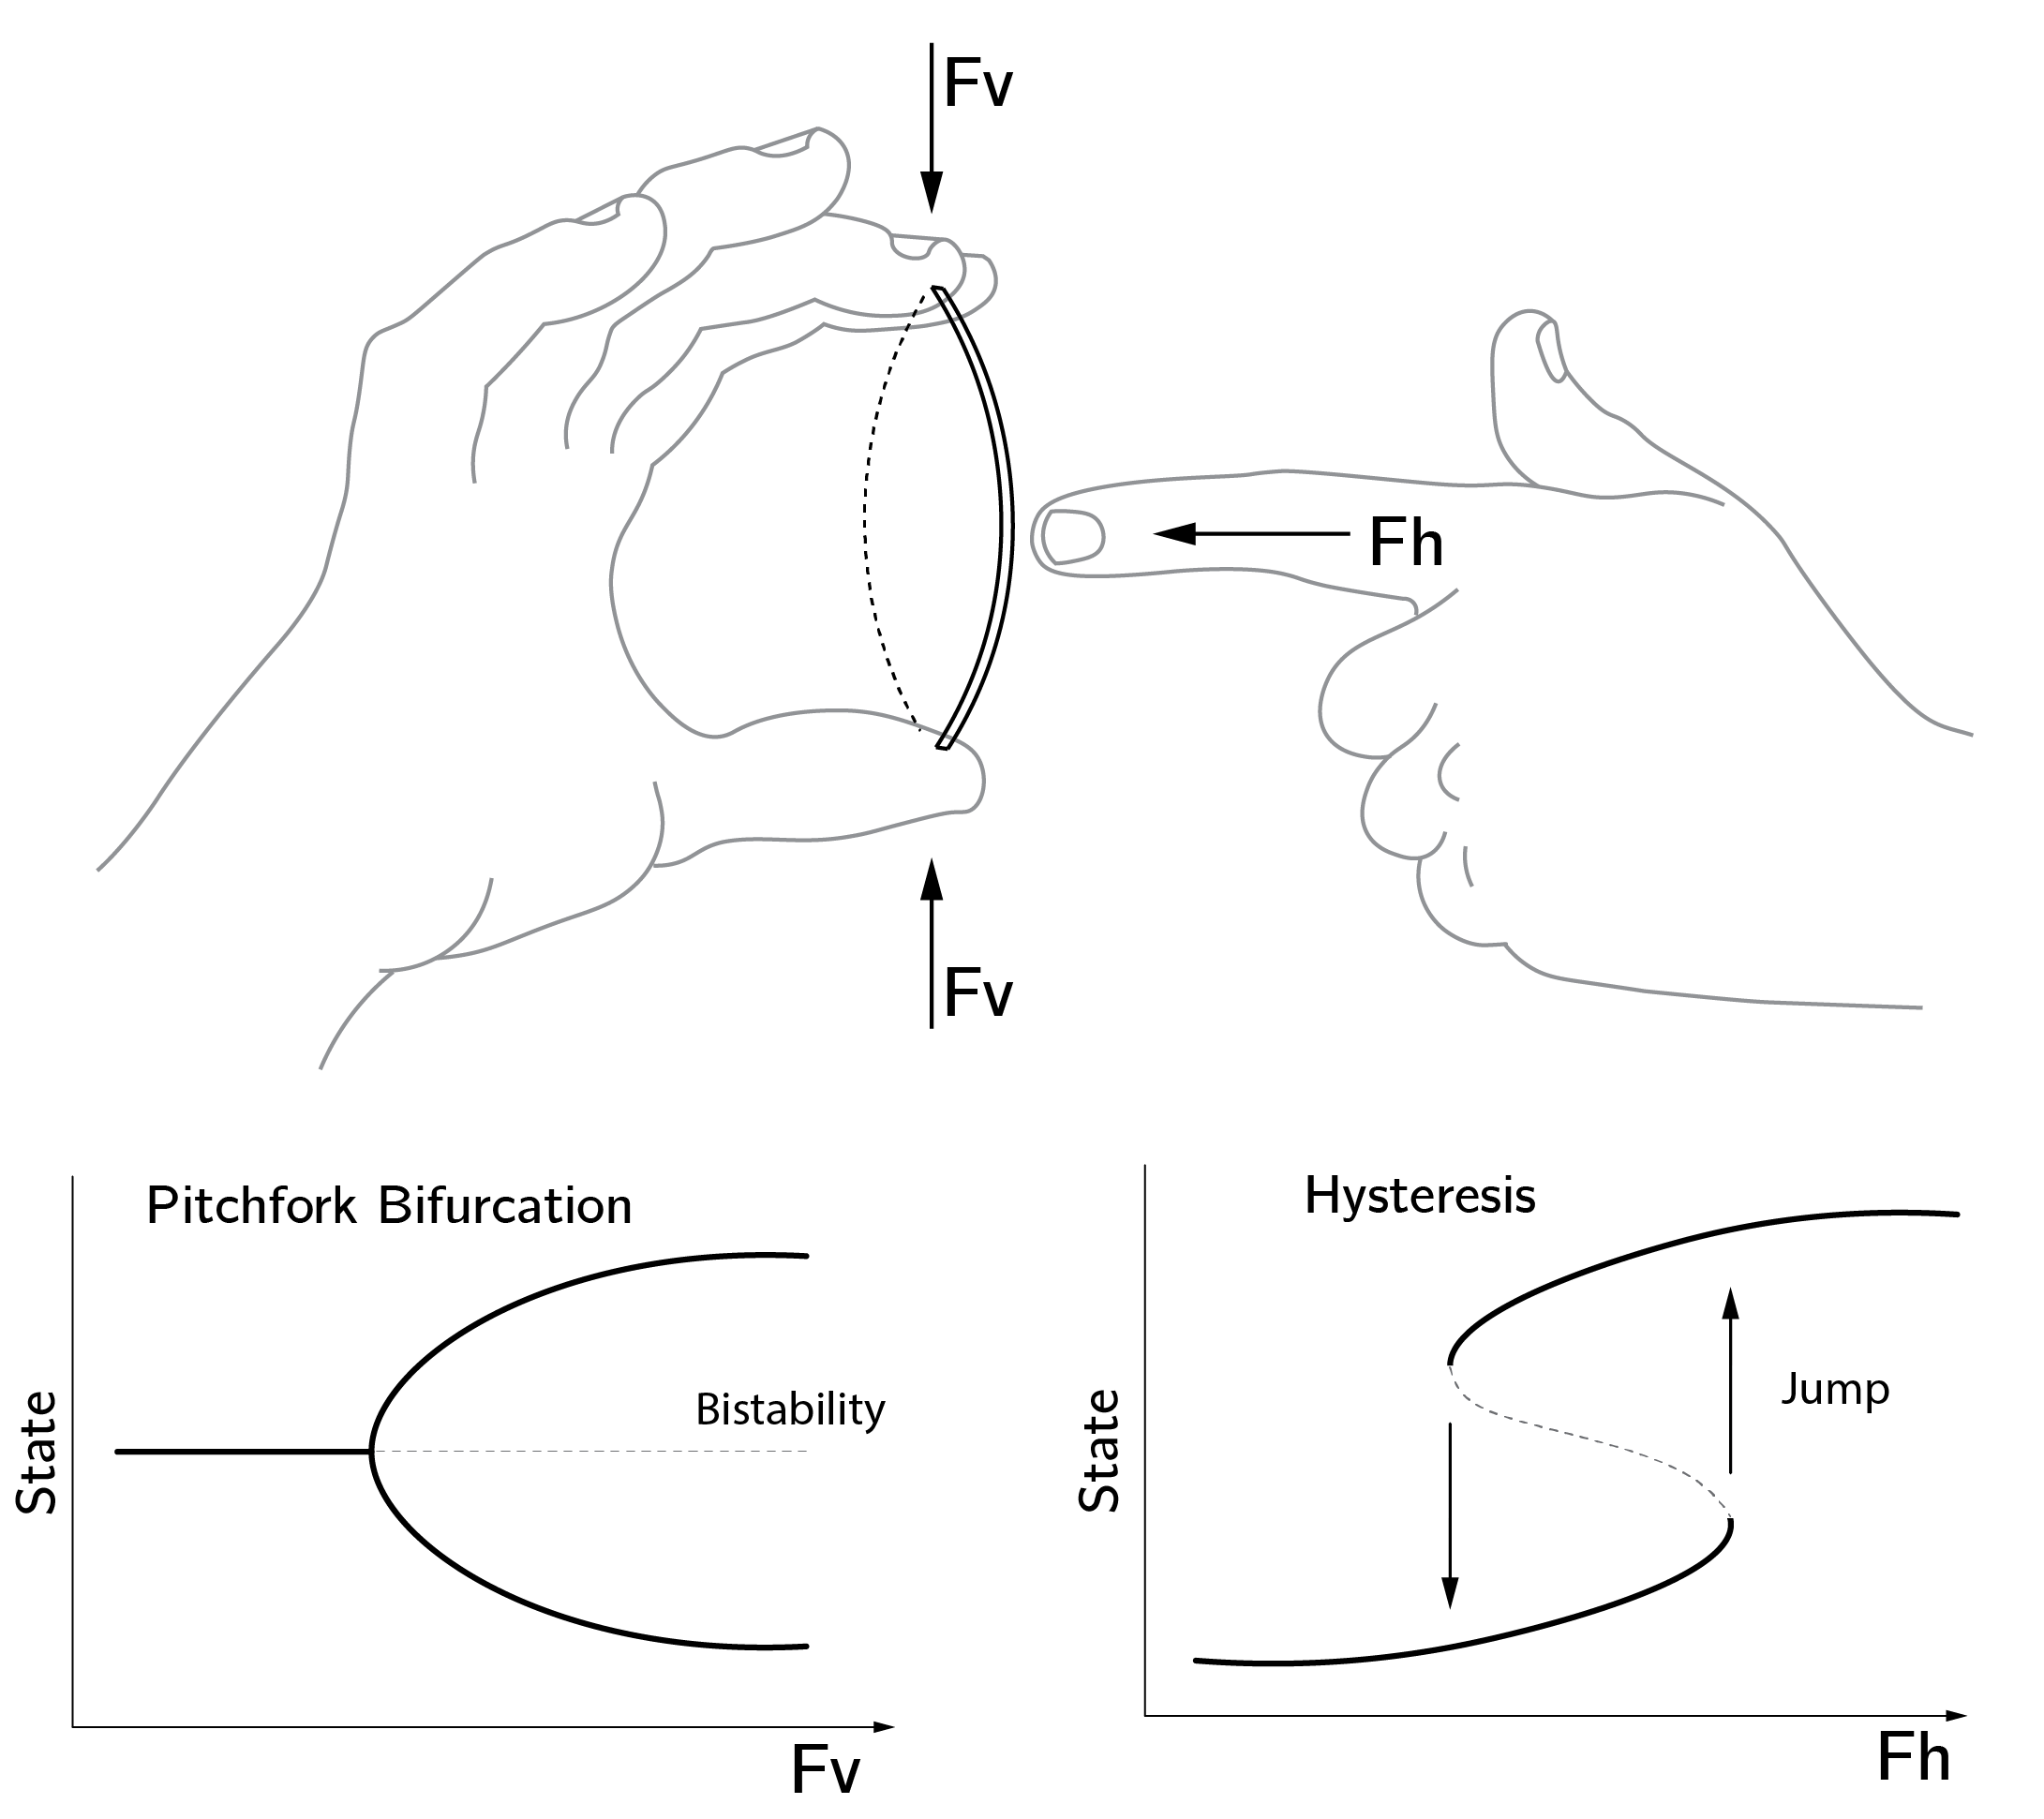
\includegraphics{media/ch3/ch3-11-may31.png}

}

\caption{\label{fig-ch3-img11-old-23}A simple business card can be used
to illustrate all the properties of the cusp (see main text).}

\end{figure}%

This seems simple, but the mathematical analysis of such elastic bending
structures is a huge topic in itself (Poston and Stewart 2014). The
freezing of water is also a cusp. As an approximation, we could say that
the density of water is the behavioral variable, temperature is the
normal variable, and pressure acts as a splitting variable (see chapter
14 of Poston and Stewart (2014), for a more nuanced analysis). It is
very instructive to study the full phase diagram of water
(figure~\ref{fig-ch3-img12-old-24}). It can be viewed as a map of the
equilibria. This type of mapping would be extremely useful in psychology
and the social sciences.

\begin{figure}

\centering{

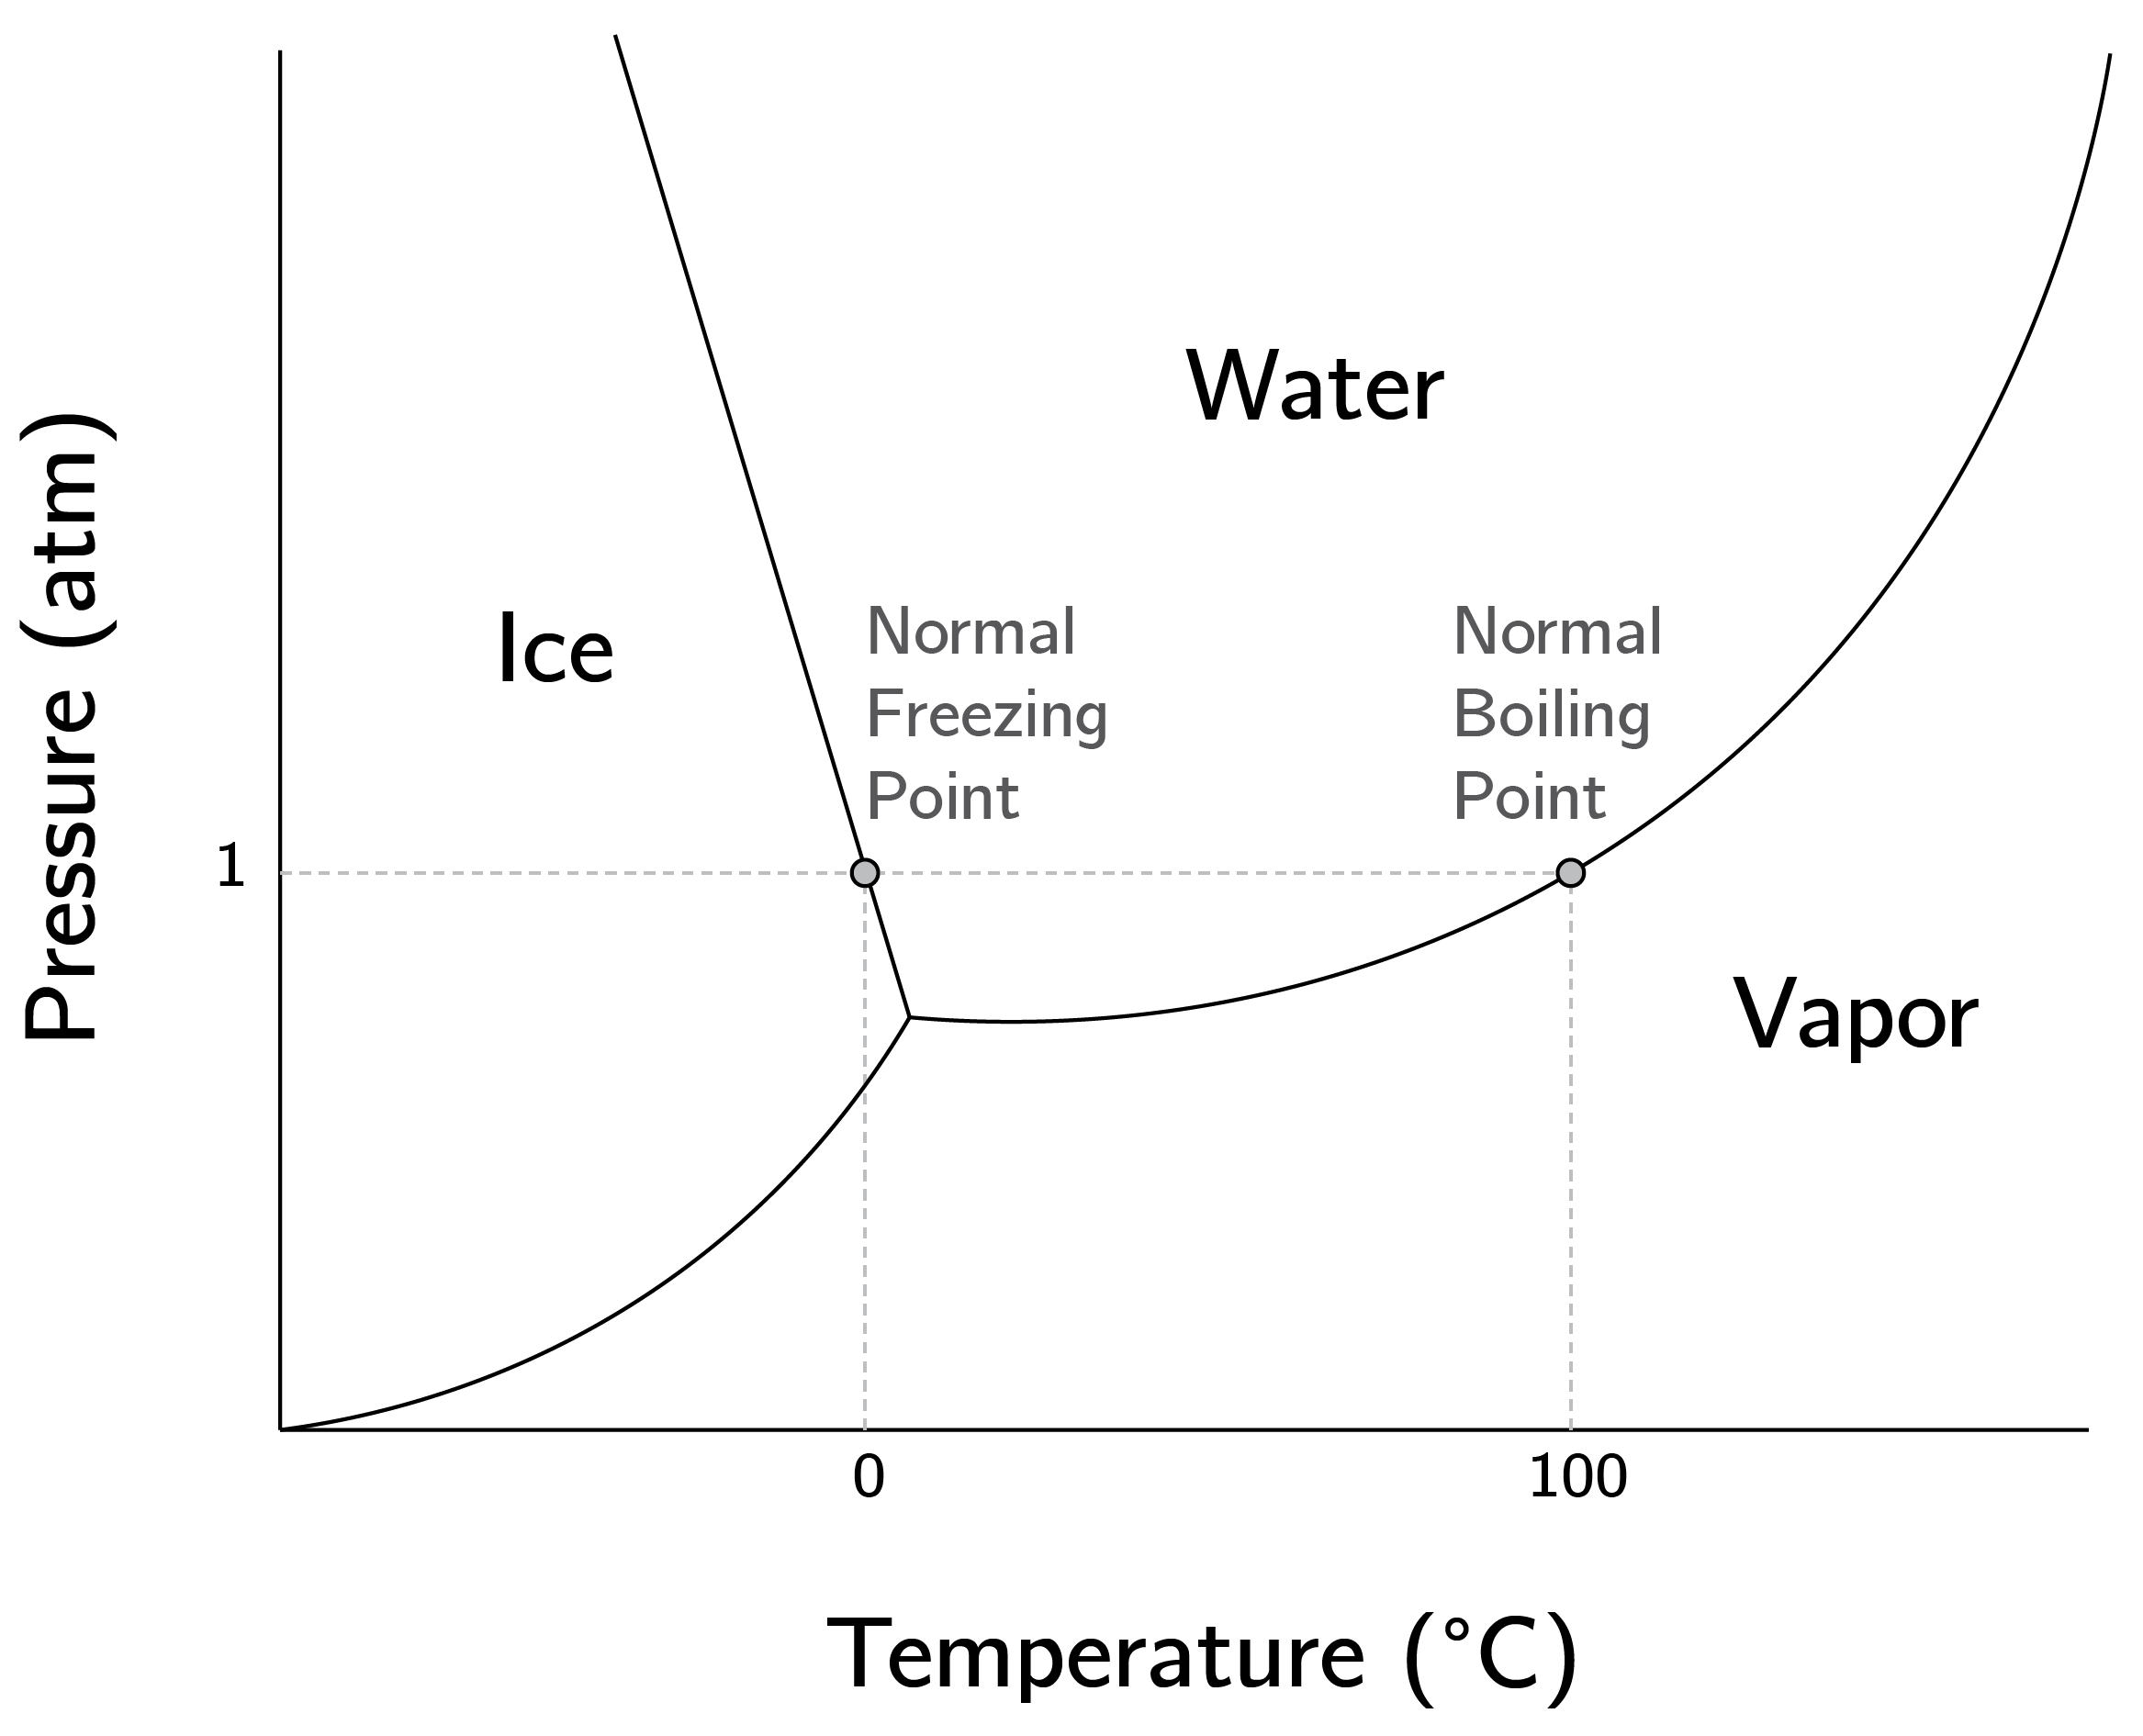
\includegraphics{media/ch3/ch3-12-may31.png}

}

\caption{\label{fig-ch3-img12-old-24}The phase diagram of water, which
summarizes the equilibria and transitions in the state of water as a
function of temperature and pressure.}

\end{figure}%

A psychological example of a cusp concerns sudden jumps in attitudes
(Latané and Nowak 1994; van der Maas, Kolstein, and van der Pligt 2003).
Attitudes will be discussed in much more detail in later chapters. In
general, we have relatively stable attitudes toward many things in life
(politics, snakes, hamburgers, and sports), but sometimes they change,
and in rare cases they change radically. For example, you may suddenly
become a conspiracy theorist, an atheist, or a vegetarian. One example
is the attitude toward abortion (figure~\ref{fig-ch3-img13-old-25}).

\begin{figure}

\centering{

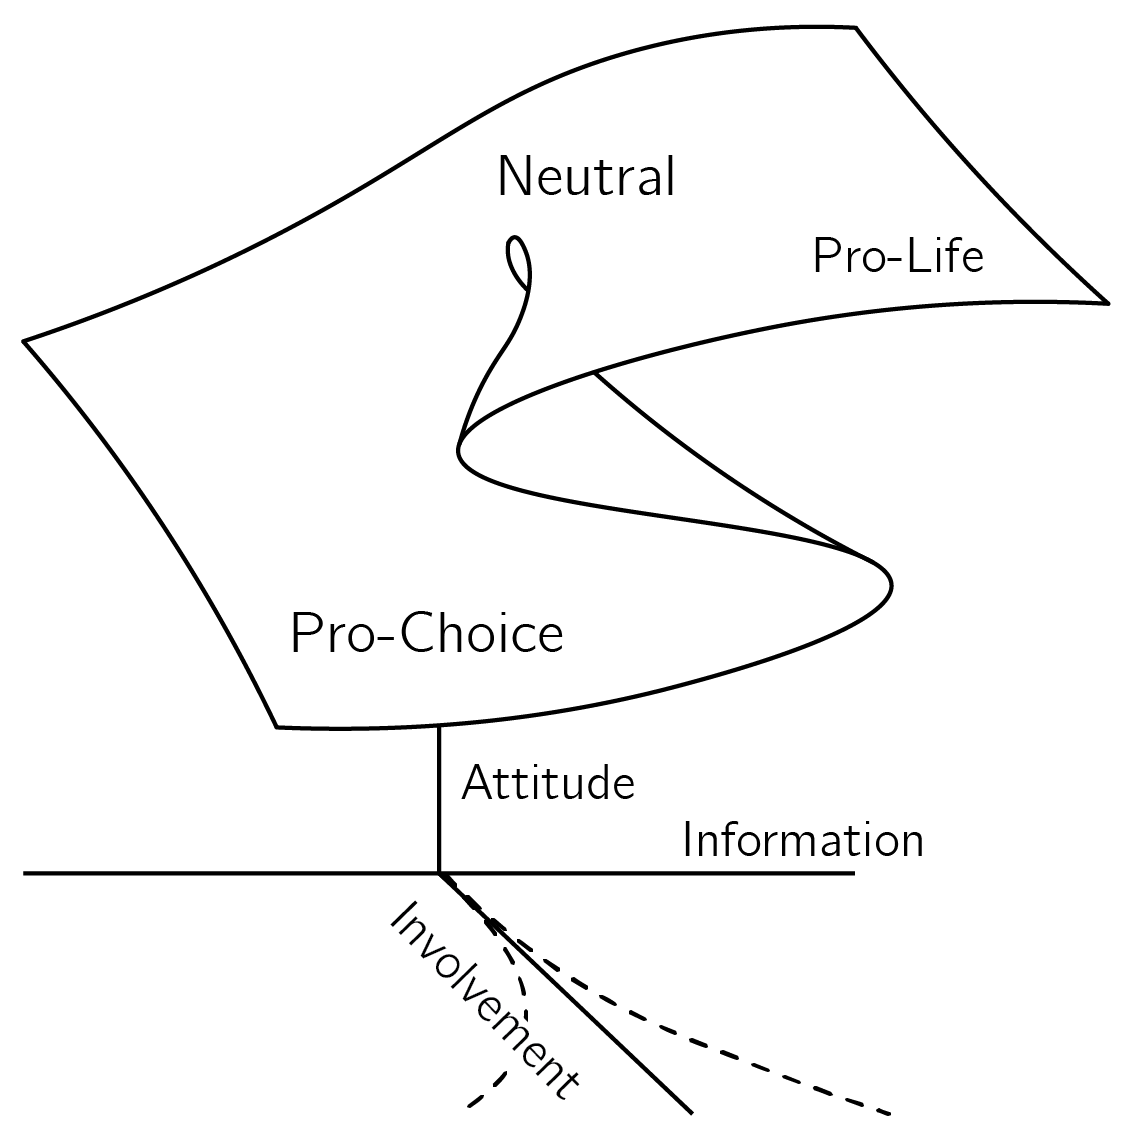
\includegraphics{media/ch3/ch3-13.png}

}

\caption{\label{fig-ch3-img13-old-25}The cusp model of attitudes (toward
abortion). Because of hysteresis, it is very difficult to persuade
highly involved people with new information, but if they change it will
be a sudden jump.}

\end{figure}%

Cusp modeling begins by defining the states of the behavioral variable.
In this case, the two states of the bistable cusp are the two opposing
positions, pro-life\footnote{Perhaps better to call this view
  anti-choice.} and pro-choice. The other state associated with
\(a = 0, b = 0\) is the neutral state, an ``I don't know'' or ``I don't
care'' position.

The normal (\(a\)) and splitting (\(b\)) variable are interpreted as
information and involvement. Information is a collection of factors that
influence whether people tend to be in the pro-life or pro-choice
position. Political and religious orientation as well as personal
experiences add to this overall factor. One way to construct this
information variable is through a factor analysis or principal component
analysis.

The splitting factor, involvement, also combines a number of effects
(importance, attention). The main idea is that there are two types of
independent variables. Some will work (mainly) along the normal axis,
and some will (mainly) impact the splitting axis.

The implications of this model are that, for low involvement, change is
continuous (figure~\ref{fig-ch3-img13-old-25}). Presenting people with
some new information supporting the pro-life or pro-choice position will
have a moderate effect. One problem, as demonstrated with the business
card, is that the uninvolved person has ``no memory.'' As soon as you
stop influencing this person, they drift to the neutral ``I don't care''
position. We have another problem when people are highly involved: they
experience hysteresis. {\marginnote{\begin{footnotesize}Because of the
hysteresis effect, it is very difficult to persuade people with new
information.\end{footnotesize}}} When this hysteresis effect is large,
persuasion just does not work. If you have been involved in political
discussions, you have probably experienced that yourself.

But if the underlying change in information is large enough, attitudes
can show a sudden jump. If they are central attitudes, they can be major
life events. There is a lot of anecdotal evidence for such transitions
(Ebaugh 1988), but it is very hard to capture such an effect in actual
time series of attitude measures. Another effect that is consistent with
the cusp model is ambivalence. {\marginnote{\begin{footnotesize}In the
cusp model of attitudes, ambivalence is not the same thing as being
neutral.\end{footnotesize}}} The neutral point is at the back of the
cusp and is associated with low involvement. Ambivalence is associated
with high involvement. Highly involved people with balanced information
(\(a = 0)\), may oscillate between extreme positions (see
figure~\ref{fig-ch4n-img2-old-50}). Finally, the pitchfork bifurcation
can explain issue or political polarization.
{\marginnote{\begin{footnotesize}When involvement increases in a group
of neutral people, for example, due to discussion, they may split into
two extreme positions (polarization).\end{footnotesize}}}

Another psychological example of the cusp-like behavior is multistable
perception. Stewart and Peregoy (1983) proposed a model in which the
perception of male face or female figure is used as a behavioral
variable, the splitting variable is the amount of detail, and the normal
variable is a change in detail related to the male/female distinction.
The results are shown in figure~\ref{fig-ch3-img14-old-26}.

\begin{figure}

\centering{

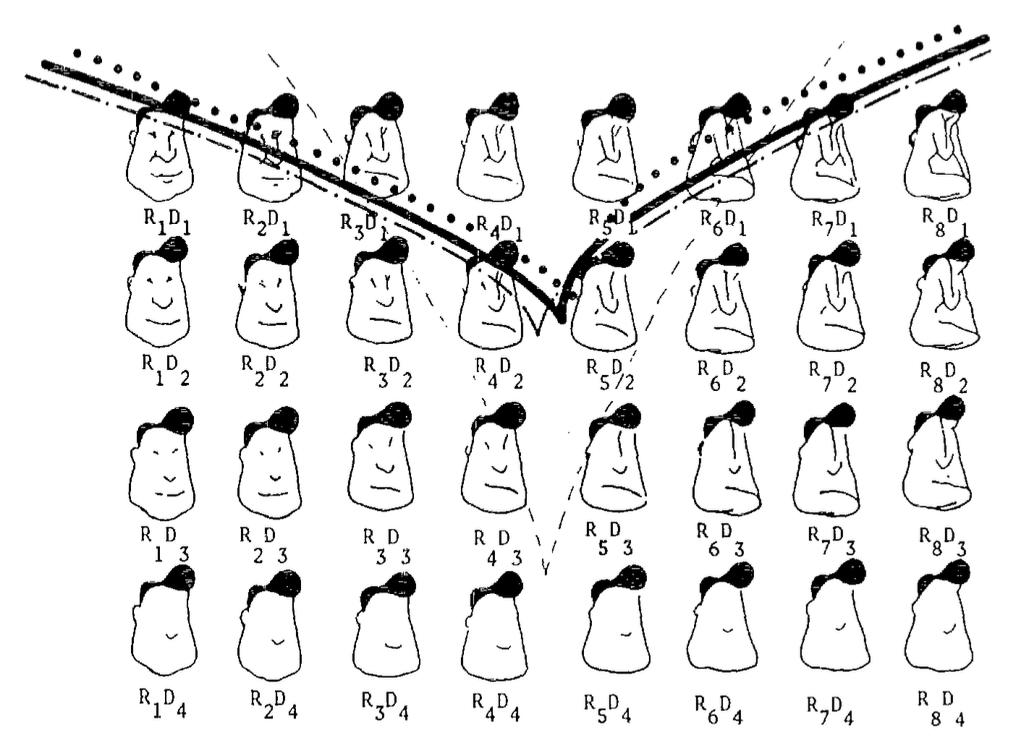
\includegraphics[width=13cm,height=\textheight]{media/ch3/image14.jpg}

}

\caption{\label{fig-ch3-img14-old-26}Multistable perceptual stimuli
positioned in the bifurcation set. The fitted bifurcation lines were
calculated using Cobb's method, which is explained in
section~\ref{sec-Cobbs-maximum-likelihood-approach}. (Adapted with
permission from Stewart and Peregoy (1983))}

\end{figure}%

\subsection{Higher-order
catastrophes}\label{sec-Higher-order-catastrophes}

Note that the cusp is made up of folds. This is best seen in the
hysteresis diagram in figure~\ref{fig-ch3-img9-old-21} (see the dotted
rectangle). Higher order catastrophes yield elements of cusps and folds.
The swallowtail catastrophe with potential function
\(V(X) = {- aX - \frac{1}{2}bX^{2} - \frac{1}{3}cX}^{3} + \frac{1}{5}X^{5}\)
consists of three surfaces of fold bifurcations meeting in two lines of
cusp bifurcations, which in turn meet in a single swallowtail
bifurcation point. We need a four-dimensional space to visualize this,
which is difficult. The Wikipedia page on catastrophe theory has some
rotating graphs that may help. The butterfly catastrophe has \(X^{6}\)
as the highest term (and four control variables).

{\marginnote{\begin{footnotesize}The butterfly catastrophe is of
interest when we observe trimodal behavior.\end{footnotesize}}} I will
discuss this catastrophe in section~\ref{sec-Tricriticality} in relation
to modeling attitudes.\footnote{I note that the butterfly catastrophe
  and the butterfly effect in chaos theory are completely unrelated
  concepts.} Other catastrophes have two behavioral variables, not one.
However, the vast majority of applications of catastrophe theory focus
on the cusp, which will also be the focus of the remainder of this
chapter. There are many good (but not easy) books that present the full
scope of catastrophe theory (Gilmore 1993; Poston and Stewart 2014).

\subsection{Other bifurcations}\label{sec-Other-bifurcations}

In contrast to bifurcation theory, catastrophe theory is limited to
structurally stable, local bifurcations.
{\marginnote{\begin{footnotesize}Bifurcation theory also deals with
nonstructurally stable bifurcations and so-called global
bifurcations.\end{footnotesize}}}

Examples of nonstructuraly stable local bifurcations are the
transcritical bifurcation (\(\frac{dX}{dt} = aX - X^{2})\) and pitchfork
bifurcation (\(\frac{dX}{dt} = bX - X^{3})\). The pitchfork is part of
the cusp and is not structurally stable because it can be perturbed by
an additional term \(a\), which, if unequal to 0, will distort the
pitchfork (see figure~\ref{fig-ch3-img15-old-27}).

\begin{figure}

\centering{

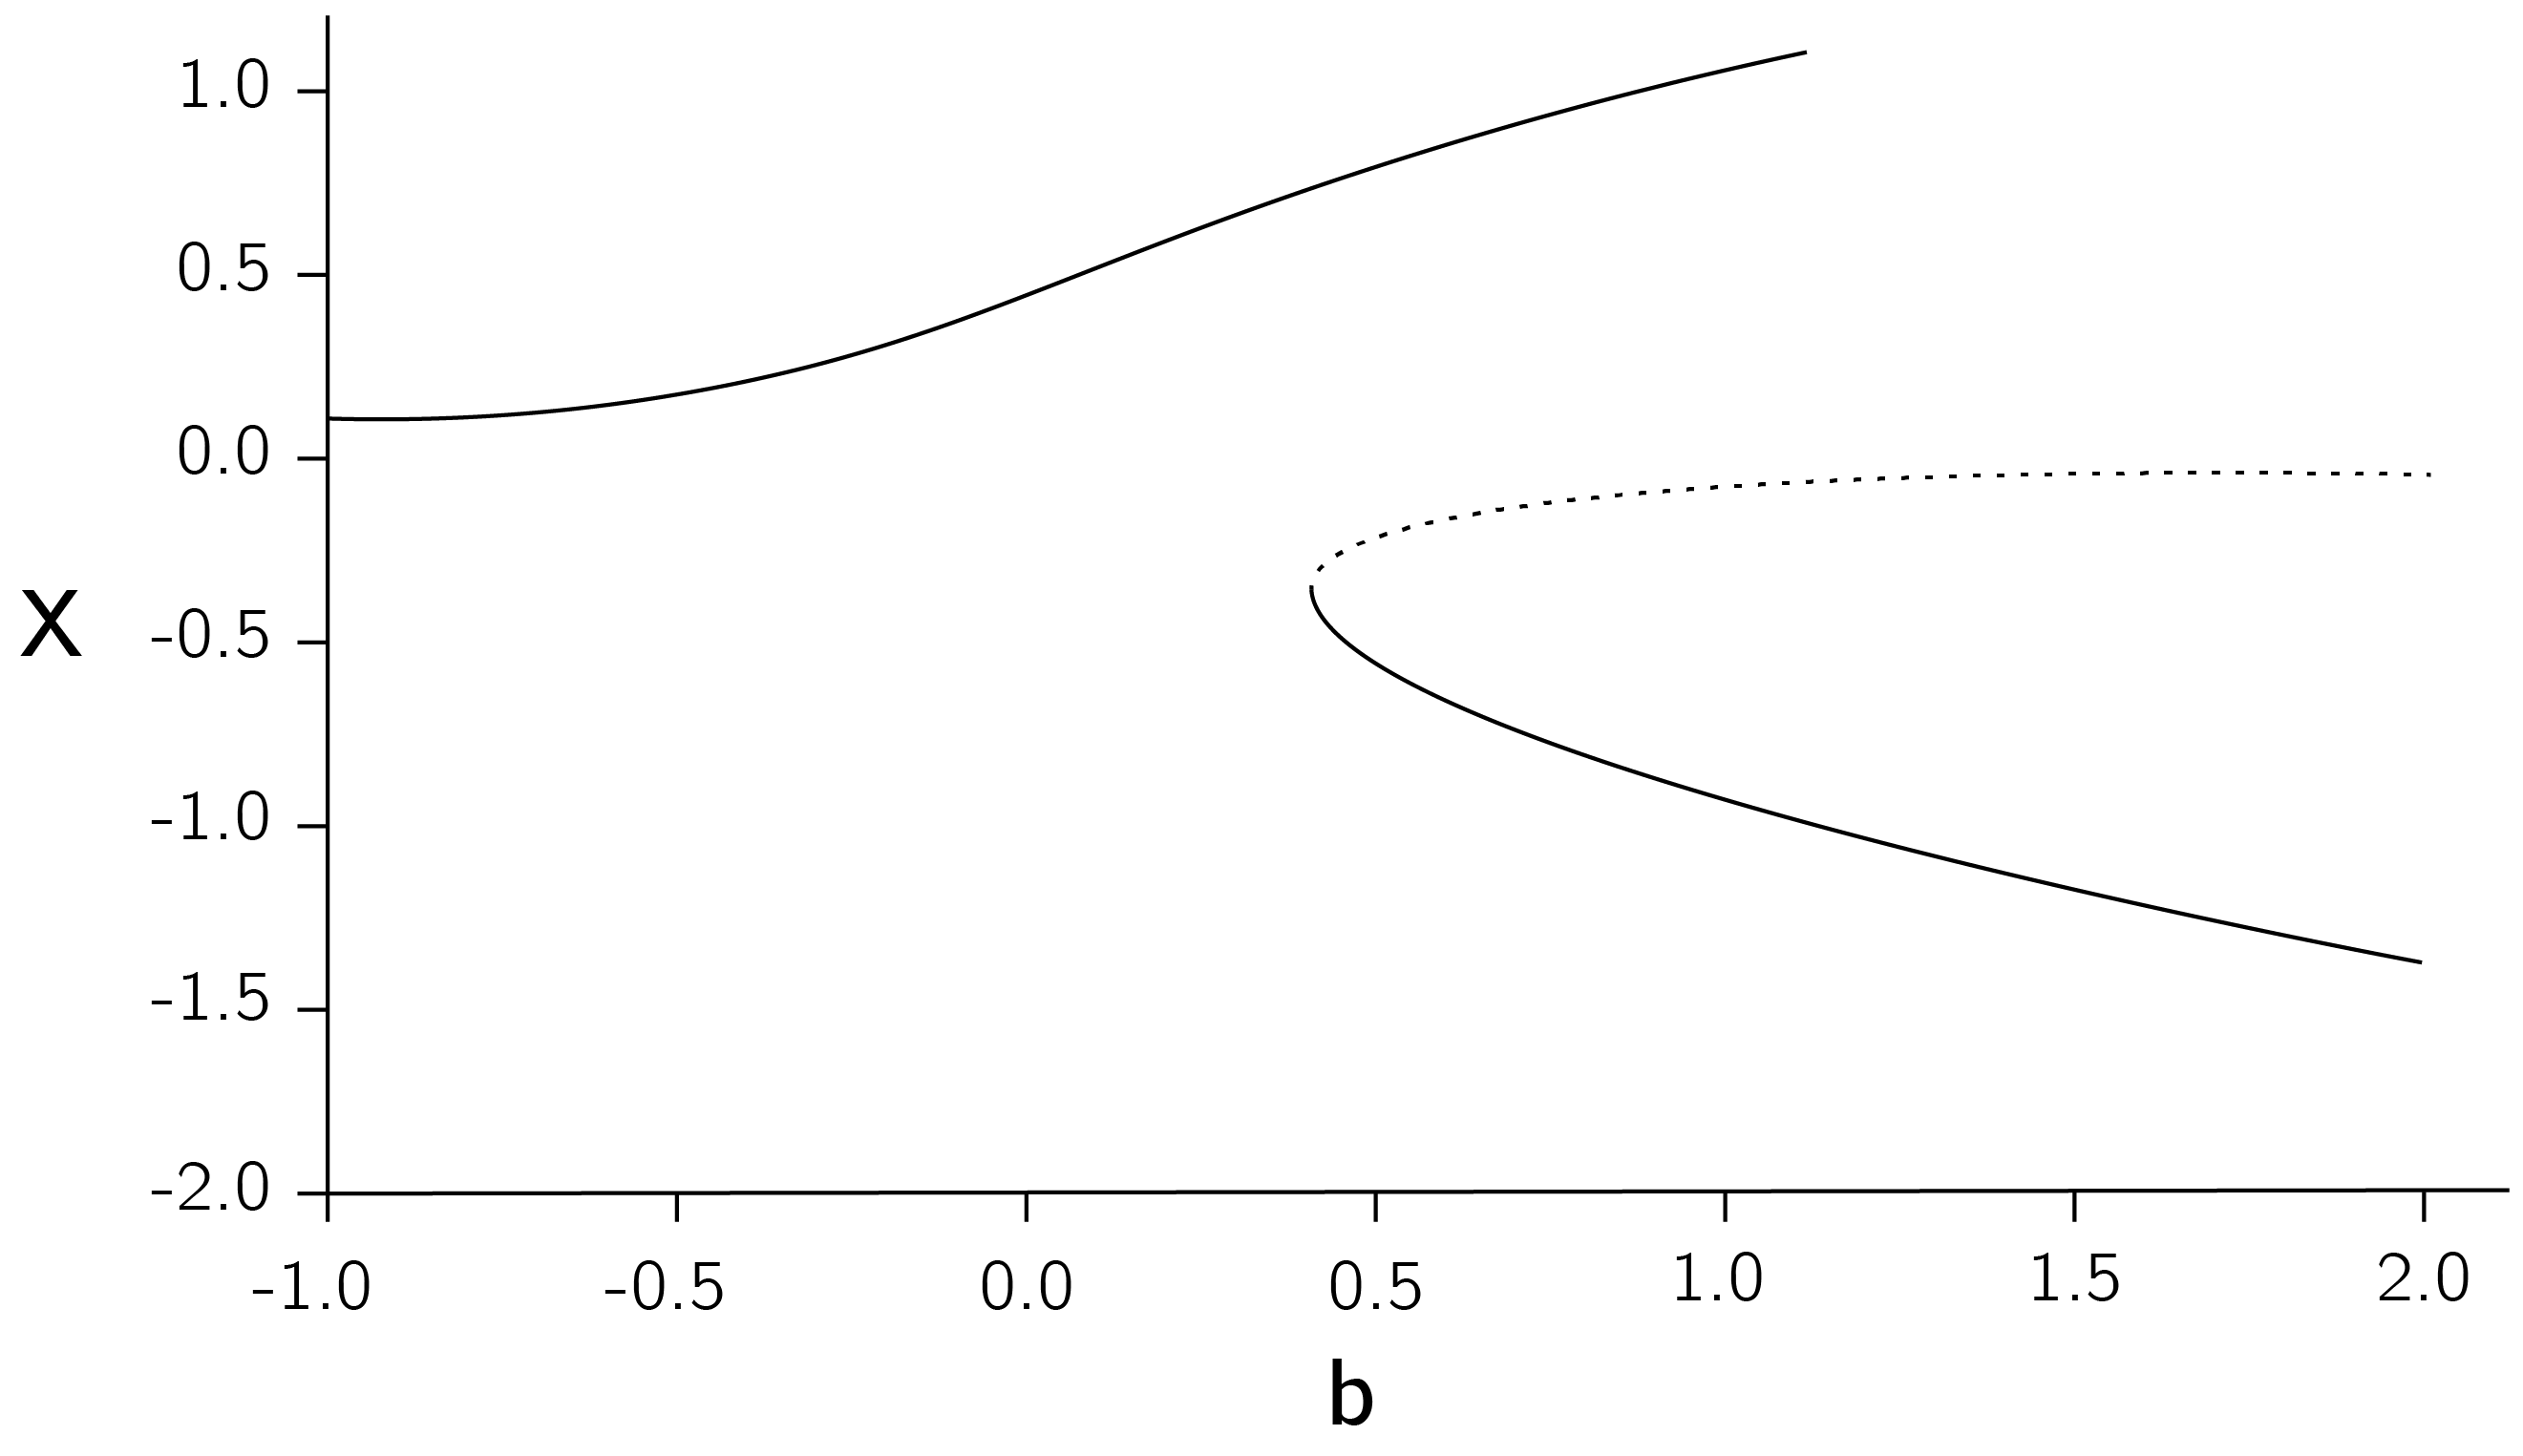
\includegraphics{media/ch3/ch3-15-may31.png}

}

\caption{\label{fig-ch3-img15-old-27}Perturbed pitchfork bifurcation
(\(a = .1\)). For \(a = 0\) we would get the pitchfork bifurcation as
shown in figure~\ref{fig-ch3-img9-old-21}. Thus, a perturbation in a
model parameter leads to qualitative change in this bifurcation, and
this is why it is not considered structurally stable.}

\end{figure}%

Another one we have already seen is the period doubling bifurcation.
This happened in the logistic map when the fixed point changed in a
limit cycle of period 2. Finally, global bifurcations cannot be
localized to a small neighborhood in the phase space, such as when a
limit cycle diverges (Guckenheimer and Holmes 1983). However, I don't
know of any applications of global bifurcations in psychology or the
social sciences.

\section{Building catastrophe
models}\label{sec-Building-catastrophe-models}

\subsection{Mechanistic models}\label{sec-Mechanistic-models}

The model of the attitude toward abortion is called a phenomenological
model, as opposed to a mechanistic model.
{\marginnote{\begin{footnotesize}In phenomenological models, we assume
the presence of a cusp, and make hypotheses about the involved
variables. In a mechanistic approach, the cusp is derived from basic
assumptions or first principles.\end{footnotesize}}}

The mechanistic approach is much more common in the physical and life
sciences. An example is the phase transition in water described by the
van der Waals equation. Poston and Stewart (2014) show how the van der
Waal equation can be reparametrized to take the form of the cusp
equation. The advantage is that we learn how temperature and pressure
are related to the control variables of the cusp. This gives us a full
understanding of the dynamics of this phase transition.

One model that I will use as a psychological model in Chapter 4,
section~\ref{sec-Analogical-modeling-Budworms-and-Beers}, is the model
of the spruce budworm outbreak, which occurs every 30 to 40 years and
results in the defoliation of tens of millions of hectares of trees
(Ludwig, Jones, and Holling 1978). The model is

\begin{equation}\phantomsection\label{eq-ch3-7-old-11}{
\frac{dN}{dt} = r_{b}N\left( 1 - \frac{N}{K} \right) - \frac{BN^{2}}{A^{2} + N^{2}}.
}\end{equation}

Where \(N\) is the size of budworm population, \(r_{b}\) is the growth
rate, \(K\) is the carrying capacity, \(B\) is the upper limit of
predation, and \(1/A\) is the responsiveness of the predator.

The first part is the logistic growth equation. \(N\) will grow to \(K\)
at a rate \(r_{b}\). Note that this is a differential equation, not a
difference equation. There is no chaos in logistic growth in continuous
time. The second part is the predation function and has a concave shape
flattening out at \(B\). The curvature of this function is determined by
\(A\). High \(A\) makes the concave shape less steep, meaning that
predation reacts rather slowly to the increase in budworms (more about
the construction of this model later).

The analytical approach to this model is to reparametrize the model so
that it takes the form of a cusp. Such reparameterizations are not so
easy to do yourself. The idea is to create a smaller set of new
variables that are functions of the model parameters. For this model a
convenient reparameterization is

\begin{equation}\phantomsection\label{eq-ch3-8-old-12}{
r = \frac{A\ r_{b}}{B}\ and\ q = \frac{K}{A}.
}\end{equation}

Using these two ``constructed'' control variables, we can depict the
bifurcation lines of the cusp as in figure~\ref{fig-ch3-img16-old-28}.

\begin{figure}

\centering{

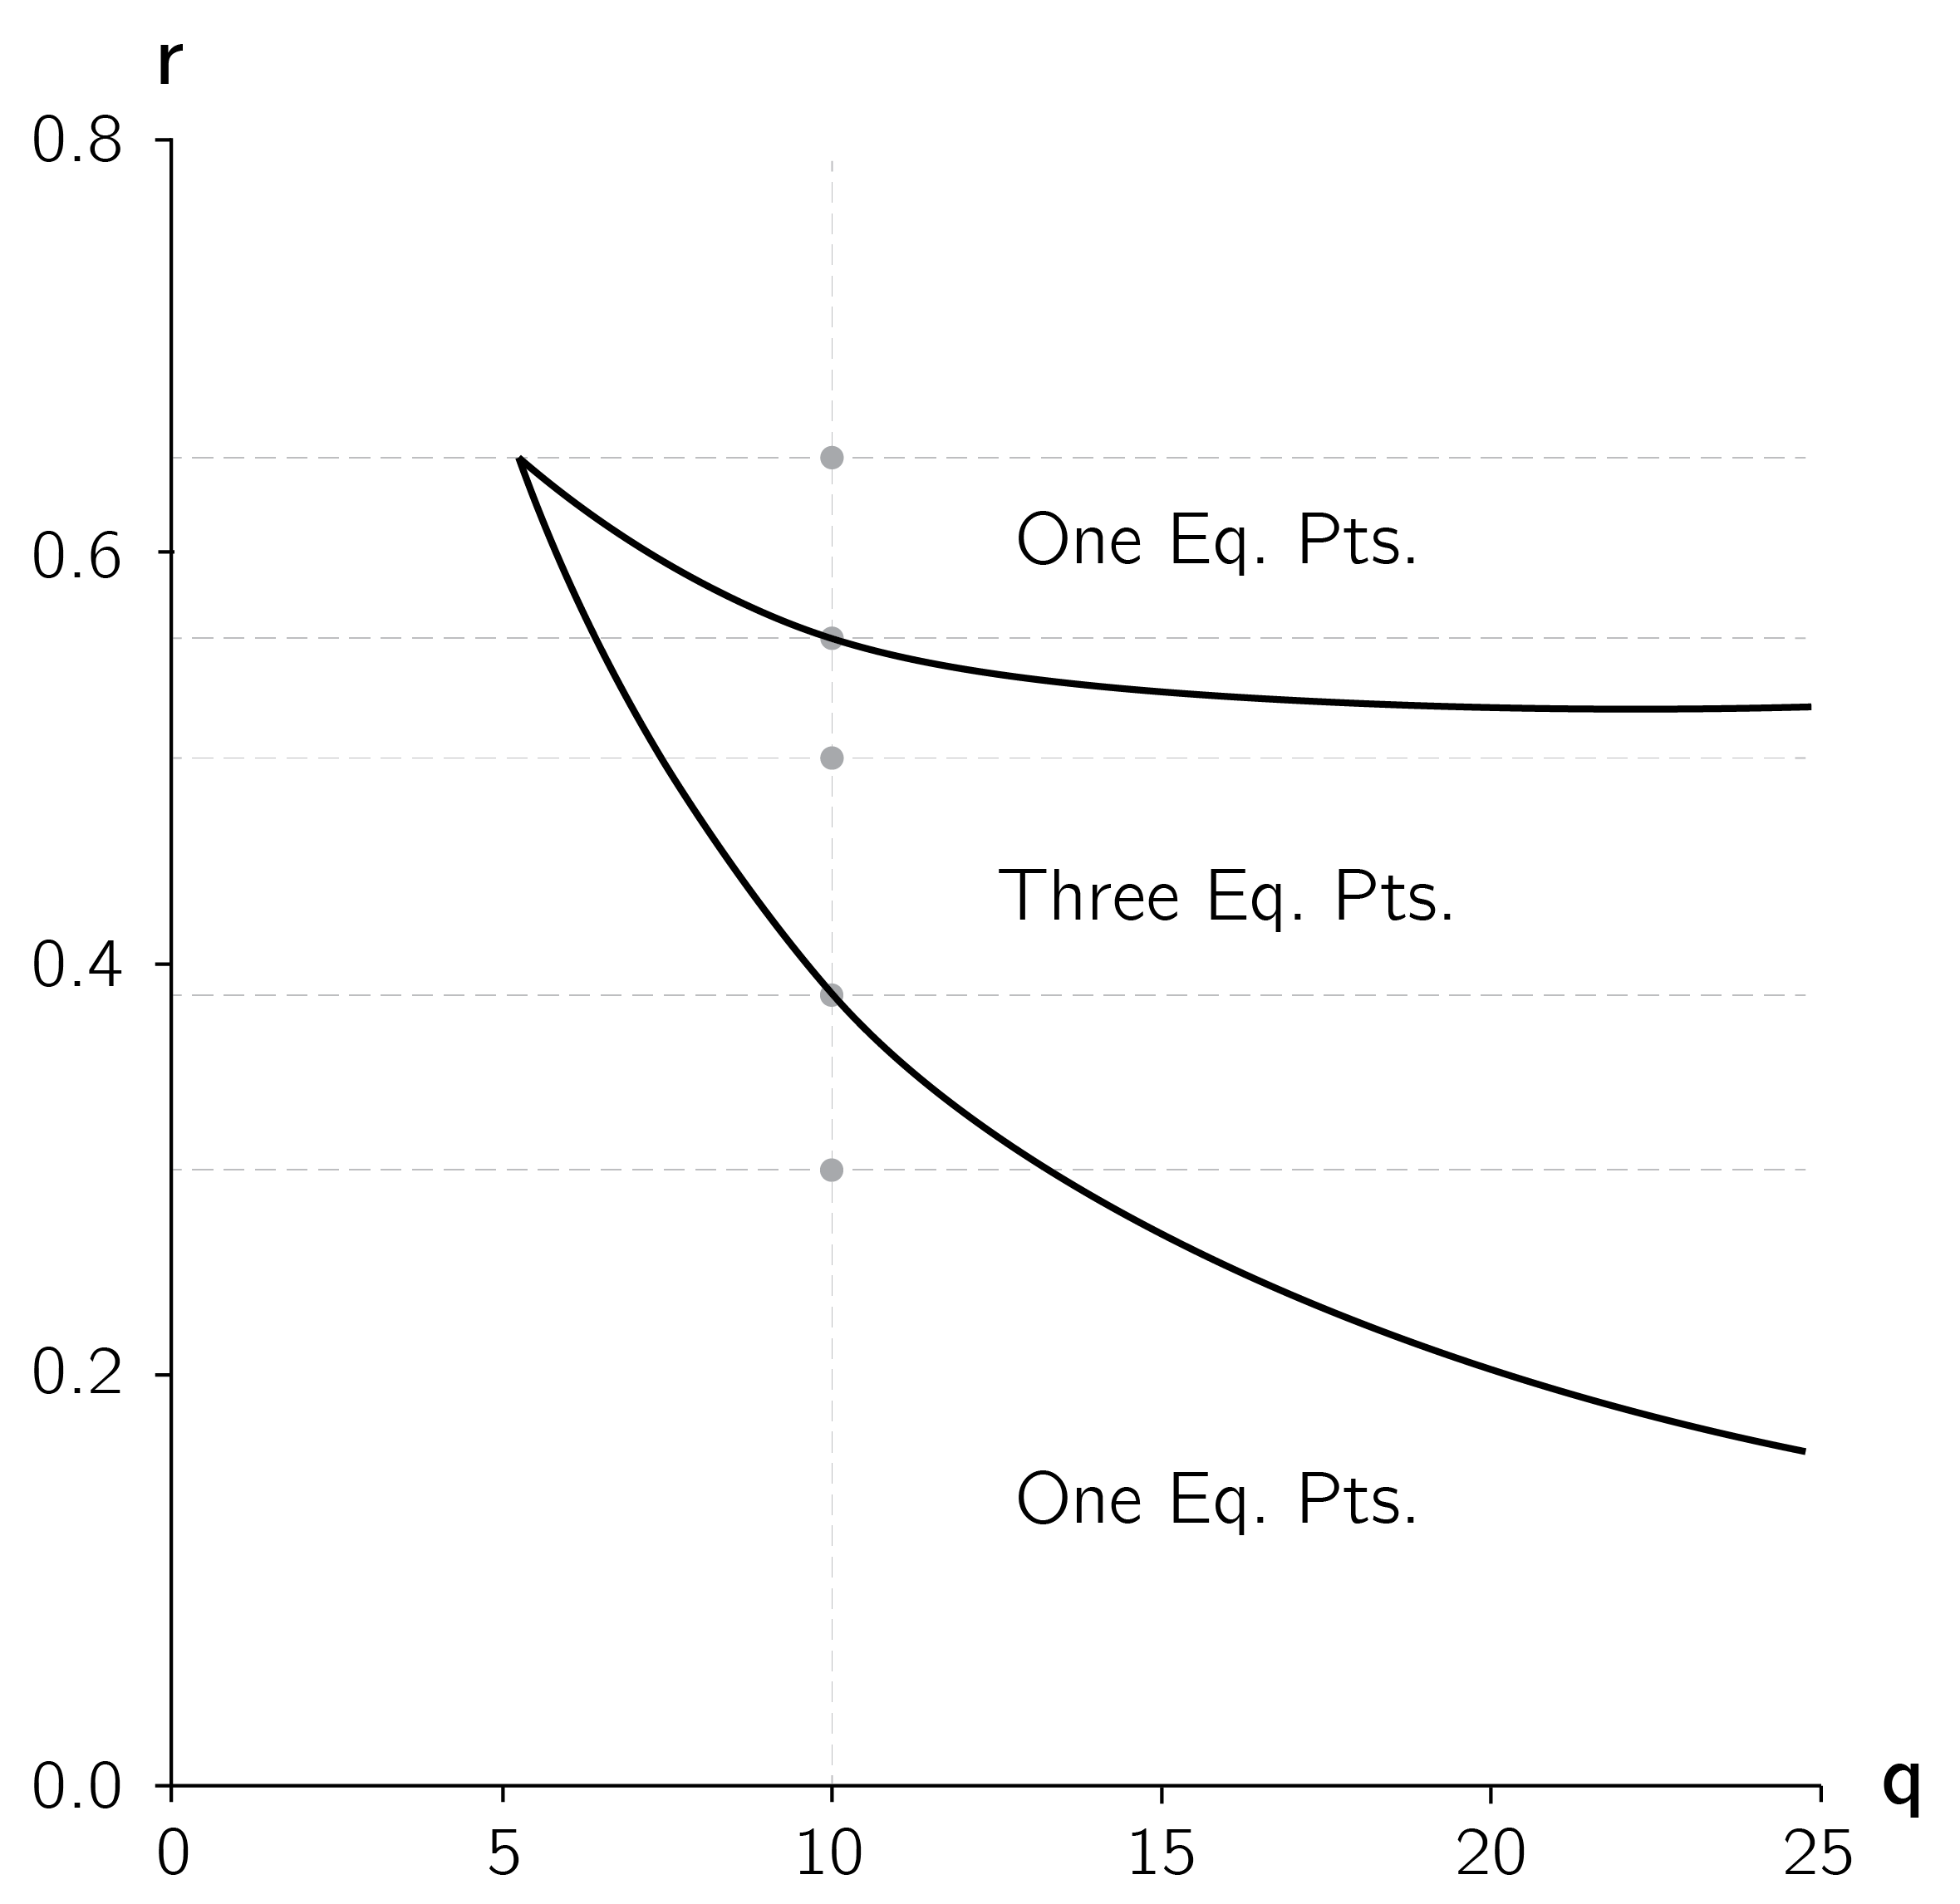
\includegraphics{media/ch3/ch3-16-may31.png}

}

\caption{\label{fig-ch3-img16-old-28}The bifurcation diagram of the
spruce budworm model.}

\end{figure}%

In later chapters we will discuss psychological examples of a
mechanistic approach, but as far as models of transitions are concerned,
these are rare. The phenomenological approach is much more common.

\subsection{Phenomenological models}\label{sec-Phenomenological-models}

The cusp model of attitude is a typical phenomenological model. We
simply assume that the cusp is a model of the attitude. Phenomenological
models are less convincing than mechanistic models because they do not
provide a deep understanding of the underlying mechanisms that drive the
system. But in psychology and the social sciences, we cannot be too
picky. Compared to many other, verbally stated attitude models, the cusp
attitude model is quite precise. It implies a number of phenomena and is
testable.

Setting up a phenomenological model is not a trivial task. I suggest
some guidelines for this. First, define the behavioral variable. It is
important to think about the bistable modes. What are they? What is the
inaccessible state in between? Can you have jumps between these states?
What is neutral state at the back of the cusp? If you cannot answer
these questions, you should reconsider whether a cusp is an appropriate
model.

Second, select the control variables. What could be a normal variable
and what could be a splitting variable? These are not easy questions.
Sometimes there are too many candidates. For the cusp model of
attitudes, instead of involvement, we could suggest interest,
importance, emotional value, etc. In this case, I think of the splitting
axis as a common factor of all these slightly different variables. In
other cases, we have no good candidates. In the example in
figure~\ref{fig-ch3-img14-old-26}, it is not clear exactly what is being
manipulated along the normal axis. If you made a choice, it is good to
check whether, at high values of the splitting values, variation of the
normal variable may lead to sudden jumps and hysteresis. Also check
whether the pitchfork bifurcation makes sense.

There is another issue here. {\marginnote{\begin{footnotesize}Control
variables in cusp models can be rotated for ease of
interpretation.\end{footnotesize}}} In some phenomenological models, the
control variables are rotated by 45 degrees. The most famous example is
Zeeman's (1976) model of dog aggression
(figure~\ref{fig-ch3-img17-old-29}).

\begin{figure}

\centering{

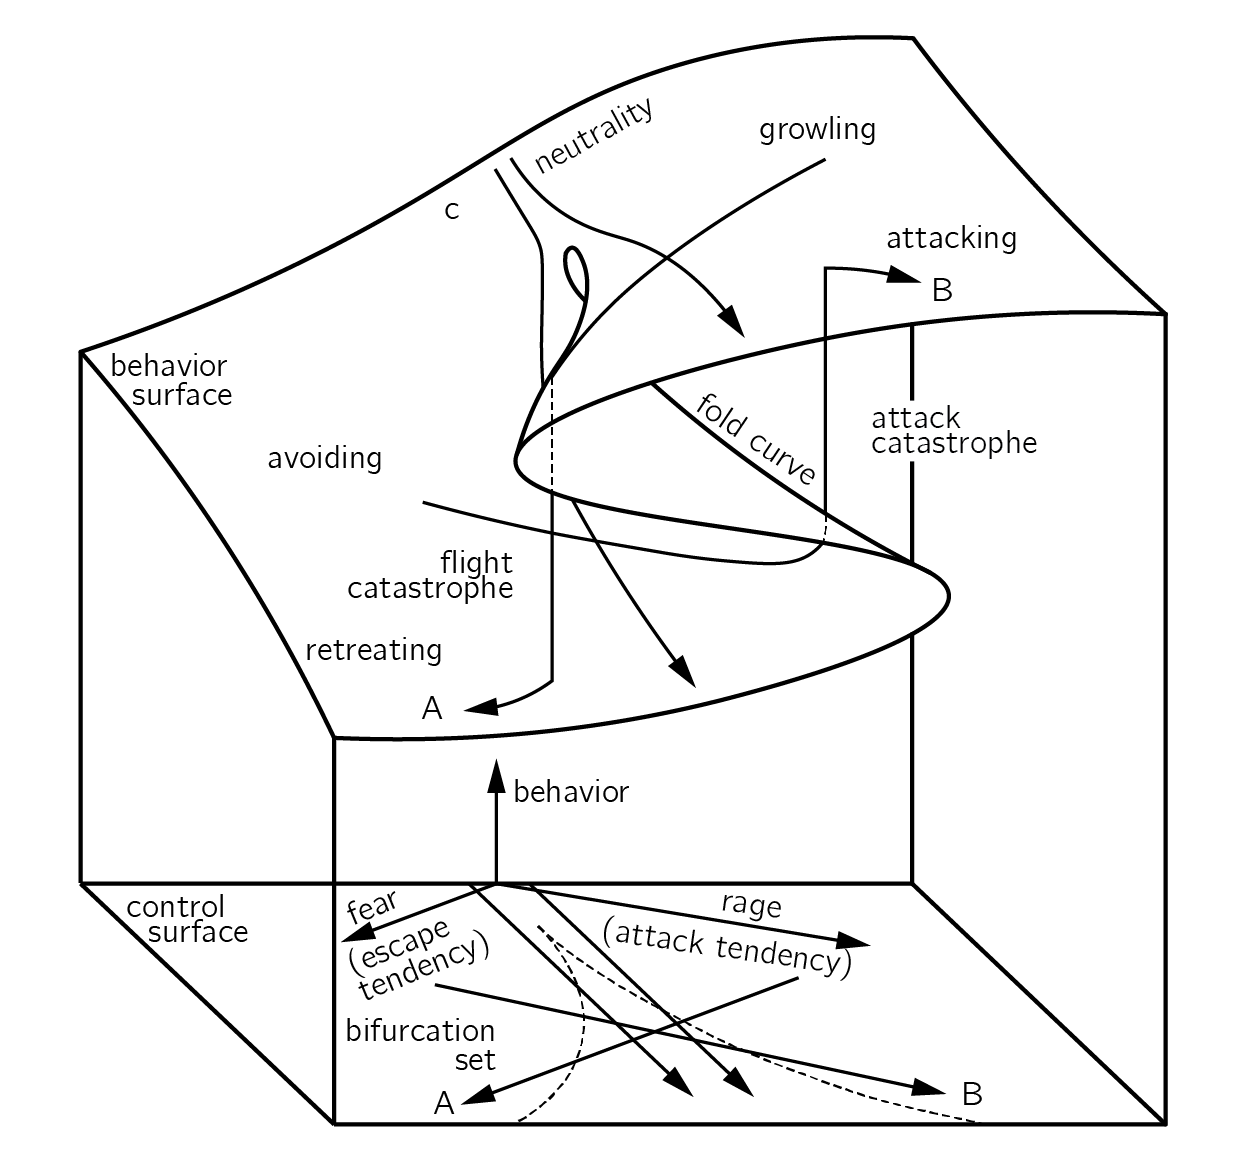
\includegraphics{media/ch3/ch3-17__figure29.png}

}

\caption{\label{fig-ch3-img17-old-29}Zeeman's dog aggression model with
rage and fear as rotated control variables.}

\end{figure}%

The control variables are fear and rage. In such a rotation the normal
variable is the difference between fear and rage, while the splitting
variable is the sum of fear and rage. Another example can be found in
our model of the speed-accuracy trade-off in reaction time tasks (Dutilh
et al. 2011). When constructing a phenomenological model, these two
options for setting the control variable should be considered.

To explain catastrophic drops in performance in work and sports, Hardy
and Parfitt (1991) proposed a cusp model with cognitive anxiety as the
splitting factor and physiological arousal as the normal factor. The
idea is that at high levels of cognitive anxiety, increases and
decreases in arousal lead to sudden changes, including a hysteresis
effect. Hardy (1996) presents further tests of this model, which has
been criticized by Cohen, Pargman, and Tenenbaum (2003). Extensions to
the butterfly model are presented in Guastello (1984) and Hardy,
Woodman, and Carrington (2004).

Cusp models have also been developed for addiction (Guastello 1984;
Mazanov and Byrne 2006). Witkiewitz et al. (2007) propose using distal
risk as the splitting axis and proximal risk as the normal axis. The
model is tested using the renowned dataset from Project MATCH, an
eight-year, multisite investigation of the effectiveness of various
treatments for alcoholism.

As a final example, I mention the model for humor presented by Paulos
(2008) in his fascinating book on mathematics and humor.\footnote{Given
  these guidelines and examples, it is an interesting exercise to
  develop one's own cusp model, for example, for falling in love. This
  is a tricky exercise.} Paulos explains his model in the context of
puns. His example is: ``Do you consider clubs appropriate for young
children?'' with the punchline ``Only when kindness fails,'' which is
probably only funny to people with children. Paulos uses the rotated
control axis as in the dog aggression model. Interpretation of the pun
is the behavioral axis. One axis represents the first meaning of
``clubs,'' the other axis represents the second meaning. The bifurcation
set represents the ambiguous region. A joke involves a jump from one
meaning to another. {\marginnote{\begin{footnotesize}The punch line
forces a catastrophic change in interpretation, accompanied by a release
of tension through laughter.\end{footnotesize}}} Paulos claims that this
cusp model combines cognitive incongruity theory, various psychological
theories of humor, and the release theory of laughter. Tschacher and
Haken (2023) propose a related complexity account of humor.

\section{Testing catastrophe
models}\label{sec-Testing-catastrophe-models}

\subsection{The catastrophe flags}\label{sec-The-catastrophe-flags}

How sudden is sudden? How can climate changes be seen as transitions
between stages (i.e., ice ages) when these transitions take hundreds of
years? Even when the ball is rolling toward its new minimum, it takes
time to roll. {\marginnote{\begin{footnotesize}Sudden transitions are
not instantaneous, but the in-between states are
unstable.\end{footnotesize}}}

But then what is the difference with an continuous acceleration, such as
we see in a logistic growth pattern? The time course of an acceleration
and a sudden, discontinuous jump may look very similar
(figure~\ref{fig-ch3-img18-old-30}).

\begin{figure}

\centering{

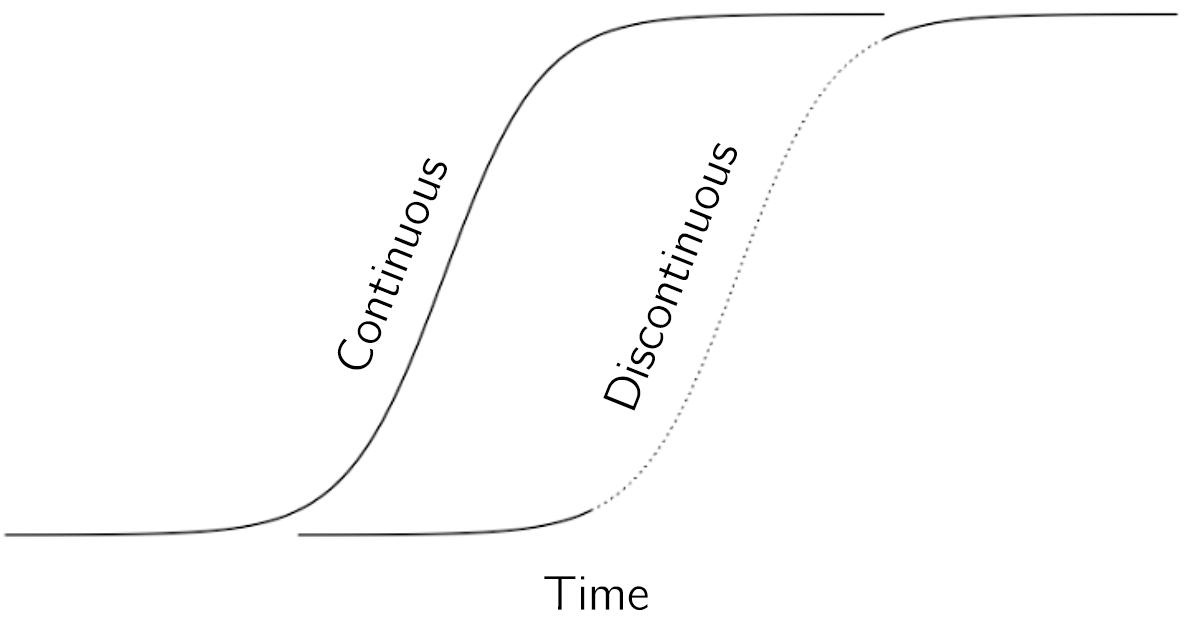
\includegraphics{media/ch3/ch3-18-may31.png}

}

\caption{\label{fig-ch3-img18-old-30}Continuous and discontinuous growth
curves my look very similar.}

\end{figure}%

In fact, in terms of time-series data, they may look exactly the same.
The main difference is that in the continuous case the intermediate
values are stable. An acceleration can be understood as a quadratic
minimum that changes its position quickly. If we stop the process by
freezing the manipulated control variable in the process, the state will
remain at an intermediate value. These intermediate values are all
stable values. If we freeze the manipulated variable in a discontinuous
process, it will continue to move to a stable state. In this case, the
intermediate state is unstable. The ball keeps rolling and unfortunately
the climate keeps changing.

In practice using time series data, this is a difficult distinction to
make. It means that simple time series are not sufficient to distinguish
accelerations from phase transitions. So how do we distinguish between
the two processes? In the context of catastrophe theory, Gilmore (1993)
proposed the catastrophe flags. These are cusp-related phenomena that
can be seen in the data. While no single one of these is sufficient to
indicate the cusp, when considered together they provide compelling
evidence for its existence.

In the following subsections, I will define the flags and illustrate
their applications in psychology using examples. The first flag is the
sudden jump.

\subsubsection{Sudden jump}\label{sec-Sudden-jump}

{\marginnote{\begin{footnotesize}The sudden jump is a large fast change
in equilibrium behavior.\end{footnotesize}}} Although the sudden jump is
not sufficient (it could be due to an acceleration), demonstrating a
sudden jump in time series is useful (also in relation to other flags).
Statistical detection of sudden jumps is possible using a number of
techniques. Figure~\ref{fig-ch3-img19-old-31} presents raw weekly
measurements of depressive symptoms using the SCL-90-R depression
subscale of a patient who gradually stopped antidepressant medication
during the study. The participant and researchers were blind to the dose
reduction scheme (Wichers, Groot, and Psychosystems 2016). One question
was whether this reduction led to a sudden jump to the depressed state.
Using a change point detection method (James and Matteson 2014), we
found a jump at 18 weeks with a bootstrapped \(p\)-value of .005 (with
the null hypothesis of no change point).

\begin{figure}

\centering{

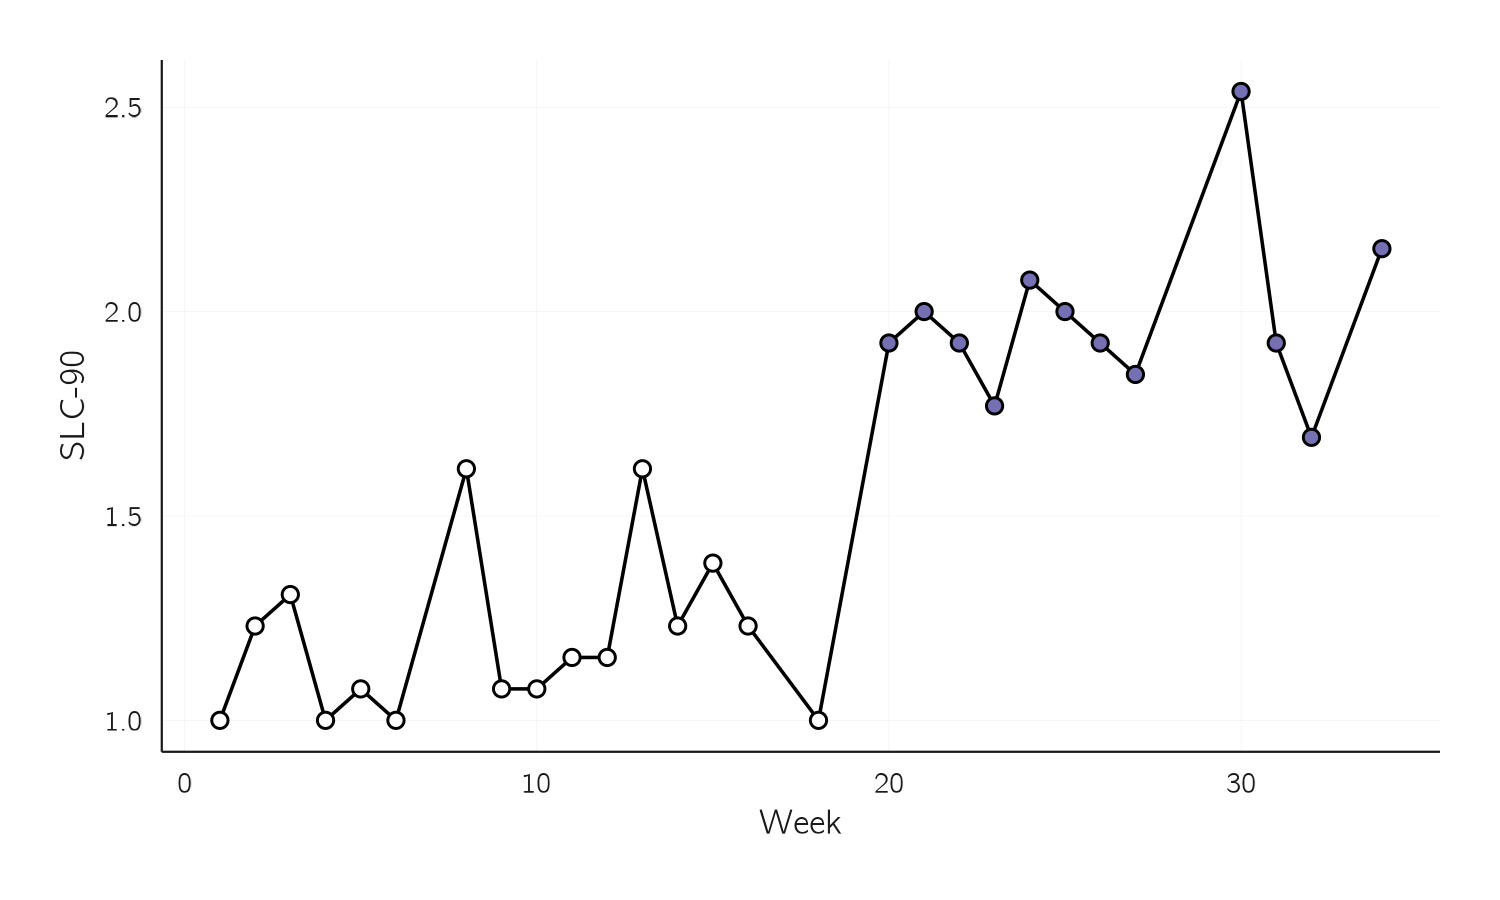
\includegraphics[width=9.375in,height=\textheight]{media/ch3/fig-ch3-img19-old-31.jpg}

}

\caption{\label{fig-ch3-img19-old-31}A sudden jump to depression (score
at the SLC-90) in a patient who gradually quit antidepressant medication
during the study.}

\end{figure}%

Many methods for change point analysis have been developed and compared
in Burg and Williams (2022).

The code for this figure is:

\begin{Shaded}
\begin{Highlighting}[]
\FunctionTok{layout}\NormalTok{(}\FunctionTok{t}\NormalTok{(}\DecValTok{1}\NormalTok{)); }\FunctionTok{par}\NormalTok{(}\AttributeTok{mar=}\FunctionTok{c}\NormalTok{(}\DecValTok{4}\NormalTok{,}\DecValTok{4}\NormalTok{,}\DecValTok{1}\NormalTok{,}\DecValTok{1}\NormalTok{))}
\NormalTok{x }\OtherTok{\textless{}{-}} \FunctionTok{read.table}\NormalTok{(}\StringTok{\textquotesingle{}data/PNAS\_patient\_data.txt\textquotesingle{}}\NormalTok{,}\AttributeTok{header=}\NormalTok{T)}
\FunctionTok{library}\NormalTok{(ecp) }\CommentTok{\# if error: install.packages(\textquotesingle{}ecp\textquotesingle{})}
\NormalTok{e1 }\OtherTok{\textless{}{-}} \FunctionTok{e.divisive}\NormalTok{(}\FunctionTok{matrix}\NormalTok{(x}\SpecialCharTok{$}\NormalTok{dep,,}\DecValTok{1}\NormalTok{),}\AttributeTok{sig=}\NormalTok{.}\DecValTok{01}\NormalTok{,}\AttributeTok{min.size=}\DecValTok{10}\NormalTok{)}
\FunctionTok{plot}\NormalTok{(x}\SpecialCharTok{$}\NormalTok{week,x}\SpecialCharTok{$}\NormalTok{dep,}\AttributeTok{type=}\StringTok{\textquotesingle{}b\textquotesingle{}}\NormalTok{,}\AttributeTok{pch=}\NormalTok{(e1}\SpecialCharTok{$}\NormalTok{cluster}\DecValTok{{-}1}\NormalTok{)}\SpecialCharTok{*}\DecValTok{16}\SpecialCharTok{+}\DecValTok{1}\NormalTok{,}\AttributeTok{xlab=}\StringTok{\textquotesingle{}Week\textquotesingle{}}\NormalTok{,}
     \AttributeTok{ylab=}\StringTok{\textquotesingle{}SLC{-}90\textquotesingle{}}\NormalTok{,}\AttributeTok{bty=}\StringTok{\textquotesingle{}n\textquotesingle{}}\NormalTok{,}\AttributeTok{main=}\StringTok{\textquotesingle{}Jump to depression\textquotesingle{}}\NormalTok{)}
\end{Highlighting}
\end{Shaded}

\subsubsection{Multimodality}\label{sec-Multimodality}

Multimodality (in the case of the cusp bimodality) is an important and
easy-to-use flag, as it can be tested with cross-sectional data. Finite
mixture models have been developed to test for multimodality in
frequency distributions (McLachlan, Lee, and Rathnayake 2019).

An example is shown in figure~\ref{fig-ch3-img20-old-32}. These data
come from a conservation anticipation task, where children have to
predict the level of water in the second glass when it is poured over.
The resulting data and the fit of a mixture of two normal distributions
are shown on the right. The data are clearly bimodal supporting the
hypothesis of a transition in conservation learning (van der Maas and
Molenaar 1992). These data were used in Dolan and van der Maas (1998) to
fit multivariate normal mixture distributions subject to a structural
equation model.

\begin{figure}

\centering{

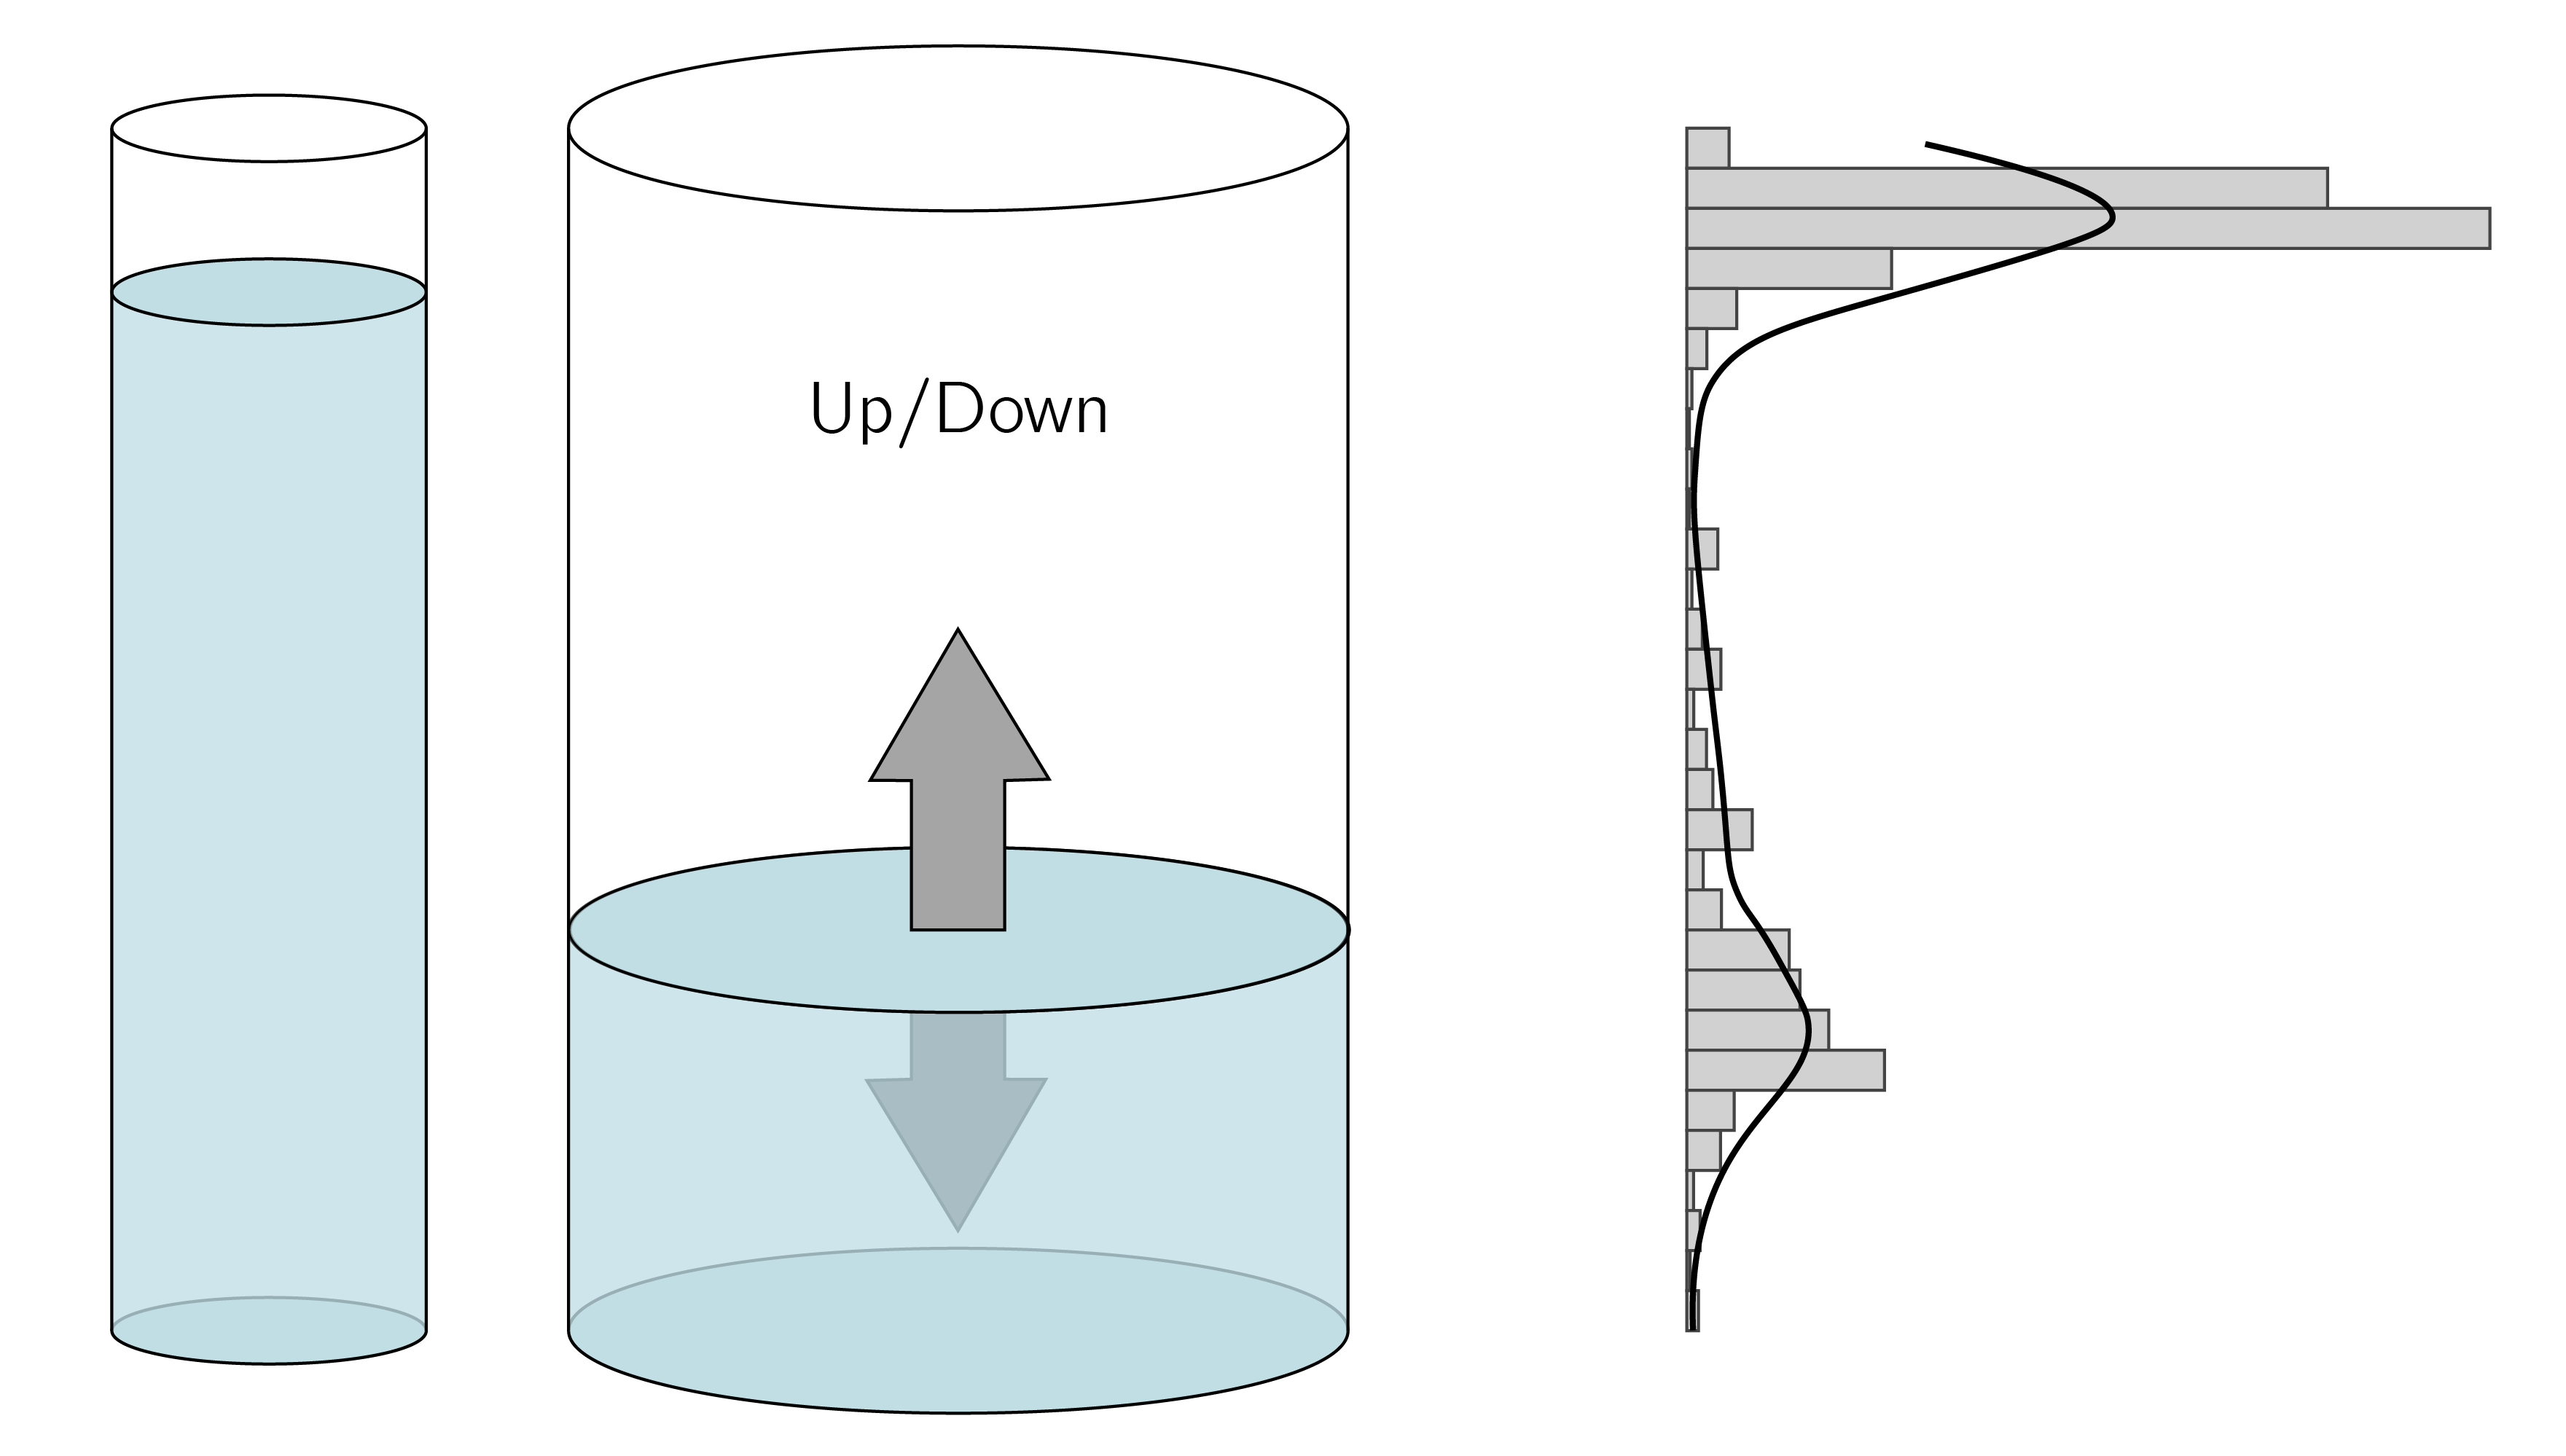
\includegraphics{media/ch3/ch3-20.png}

}

\caption{\label{fig-ch3-img20-old-32}Bimodality in the expected heights
of water when it is poured into a wider glass. This variation of the
Piagetian maintenance task is used with children ages five to eight.}

\end{figure}%

The code is:

\begin{Shaded}
\begin{Highlighting}[]
\NormalTok{x}\OtherTok{=}\FunctionTok{unlist}\NormalTok{(}\FunctionTok{read.table}\NormalTok{(}\StringTok{\textquotesingle{}data/conservation\_anticipation\_item3.txt\textquotesingle{}}\NormalTok{))}
\FunctionTok{library}\NormalTok{(mixtools) }\CommentTok{\# if error: install.packages(\textquotesingle{}mixtools\textquotesingle{})}
\NormalTok{result}\OtherTok{=}\FunctionTok{normalmixEM}\NormalTok{(x)}
\FunctionTok{plot}\NormalTok{(result,}\AttributeTok{whichplot=}\DecValTok{2}\NormalTok{,}\AttributeTok{breaks=}\DecValTok{30}\NormalTok{)}
\end{Highlighting}
\end{Shaded}

There is a whole field in statistics focused on multimodality, mixtures,
and clustering. There are some blogs that present overviews of the
relevant R packages (Arnaud 2021). Several detailed examples from
psychology, using hidden Markov models, are presented in Visser and
Speekenbrink (2022).

{\marginnote{\begin{footnotesize}The advantage of multimodality over the
sudden jump is that we can test it with cross-sectional
data.\end{footnotesize}}} To capture a sudden jump in a development
process, you need a lot of high-frequency data. Sudden shifts in opinion
are also rare. But it is easy to collect data on large numbers of people
who are asked to make judgments about statements on an issue such as
abortion. If these judgments are bimodally distributed, this is
consistent with a phase transition. Bimodal data may also be produced by
a process of acceleration, with time series consisting mainly of data
values before and after the acceleration. So, bimodality is not
sufficient. It can be considered necessary, so I always suggest starting
with cross-sectional multimodal studies. If they fail, you might
reconsider your hypothesis. I have often looked for multimodality in
measures of arithmetic learning and never found anything convincing,
which made me rethink my hypothesis.

\subsubsection{Inaccessibility}\label{sec-Inaccessibility}

Inaccessibility means that certain values of the behavioral variable are
unstable. The business card is a good example. Given some vertical
pressure, we can try what we want but we cannot force the card to stay
in the middle position; it is unstable.
{\marginnote{\begin{footnotesize}Inaccessibility is relevant to reject
the alternative hypothesis that the sudden jump and bimodality are due
to an acceleration.\end{footnotesize}}}

In Experiment 2 of Dutilh et al. (2011), we focused on this flag. Our
hypothesis was that in simple choice response tasks there is a phase
transition between a fast-guessing state and a slower stimulus-driven
response state. The idea is that if we force subjects to speed up, there
will be a catastrophic decline in performance (from almost 100\% correct
to 50\% correct).

We created a game in which subjects responded to a series of simple
choice items (a lexical decision task). The length of the series was not
known to the subject. At the end of a series, they were rewarded
according to how close their percentage correct was to 75\%. Speed was
also rewarded, but much less. So, we asked the subject to be in the
inaccessible state. The alternative hypothesis, based on information
accumulation models, was that there was no phase transition and that
responding with 75\% accuracy required the correct setting of a boundary
(see section~\ref{sec-Response-time-models}).

It appeared that subjects solved the task by switching between the
fast-guessing mode and the slower stimulus-controlled mode, even when
instructed according to the alternative model. Thus, the 75\%
intermediate state appeared to be unstable.

\subsubsection{Divergence}\label{sec-Divergence}

Divergence or the pitchfork bifurcation, the splitting up of an
equilibrium, requires the manipulation of the splitting variable. In the
case of attitudes, we hypothesize this to be involvement or some related
variable. In van der Maas, Kolstein, and van der Pligt (2003), we
reanalyzed a dataset from Stouffer et al. (1949), which Latané and Nowak
(1994) presented as evidence for the cusp model. The attitude concerned
demobilization (from 0, unfavorable, to 6, favorable), and respondents
were asked to indicate how strongly they felt about their answer (from
intensity 0 to intensity 5). For low intensities of feeling, the data
are normally distributed whereas for higher intensities, data are
bimodally distributed (see figure~\ref{fig-ch3-img21-old-33}).
{\marginnote{\begin{footnotesize}After testing for multimodality,
testing for divergence is a sensible next step.\end{footnotesize}}}

\begin{figure}

\centering{

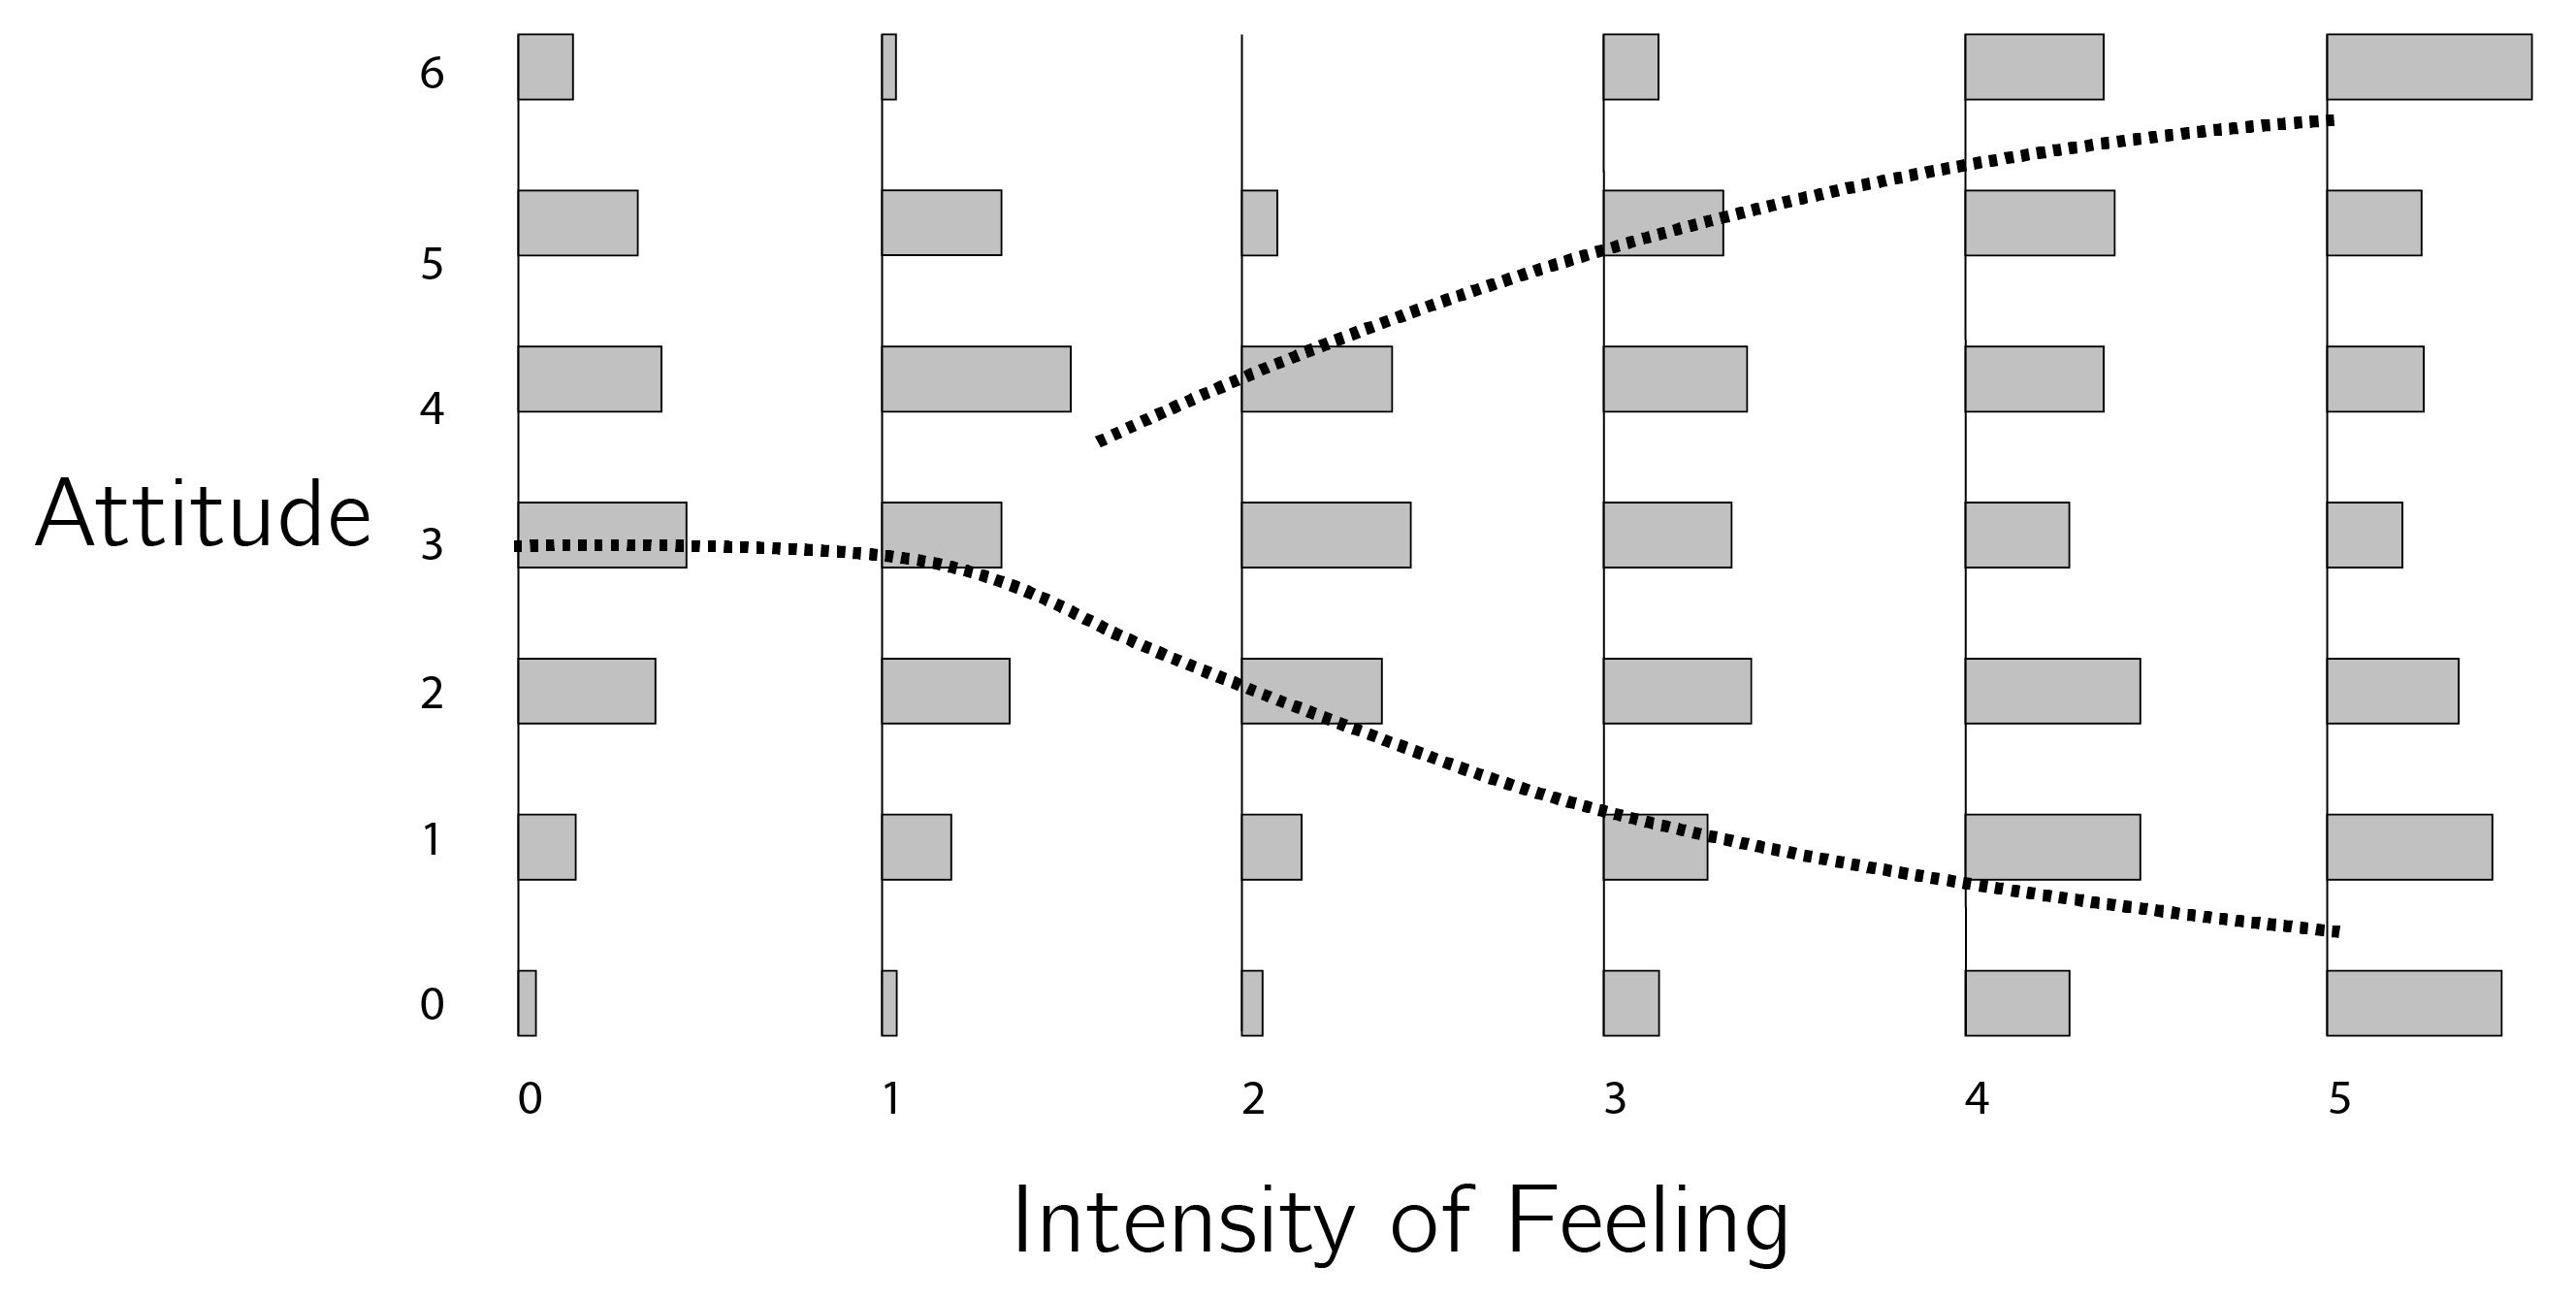
\includegraphics{media/ch3/ch3-21-may31.png}

}

\caption{\label{fig-ch3-img21-old-33}The pitchfork bifurcation in
attitudes. The dotted lines represent the fit of the cusp model to these
data. This technique will be discussed in
section~\ref{sec-Fitting-the-cusp-to-crosssectional-data}.}

\end{figure}%

\subsubsection{Hysteresis}\label{sec-Hysteresis}

{\marginnote{\begin{footnotesize}Hysteresis, the lagging behind of the
sudden jump, requires sophisticated manipulation of the normal control
variable.\end{footnotesize}}} To test for hysteresis, we need to slowly
increase and decrease this variable and test whether sudden jumps occur
with a delay. We have demonstrated hysteresis in proportional reasoning
using Piaget's balance scale test in which a specific dimension
(distance from the fulcrum) was systematically varied (Jansen and van
der Maas 2001). We also hypothesized that speeding up subjects in
response time tasks would eventually lead to a catastrophe in accuracy.
To support this claim, we demonstrated bimodality in response times and
hysteresis in the speed-accuracy trade-off (Dutilh et al. 2011). To
support the cusp model of multistable perception, we used the quartet
motion paradigm (Ploeger, van der Maas, and Hartelman 2002). In this
perceptual paradigm two lights are presented simultaneously, first a
pair from two of the diagonally opposite corners of the rectangle, and
then a second pair from the other two diagonally opposite corners of the
rectangle. Usually, either vertical or horizontal apparent motion is
perceived. By gradually increasing or decreasing the aspect ratio (i.e.,
the ratio of height to width of the quartet), hysteresis in the jumps
between the two percepts was demonstrated (see
figure~\ref{fig-ch3-img22-old-34}).

In Ploeger, van der Maas, and Hartelman (2002), we used a special
design, the method of modified limits, to rule out the alternative
explanation that hysteresis is simply due to delayed responses. It could
be that the switches always occur in the middle (at an aspect ratio of
1), but the self-report is delayed. In the modified limits method,
subjects do not respond during a trial, only after the entire trial. By
varying the length of the trials, it is possible to determine at which
parameter value the subject perceives a switch.

\begin{figure}

\centering{

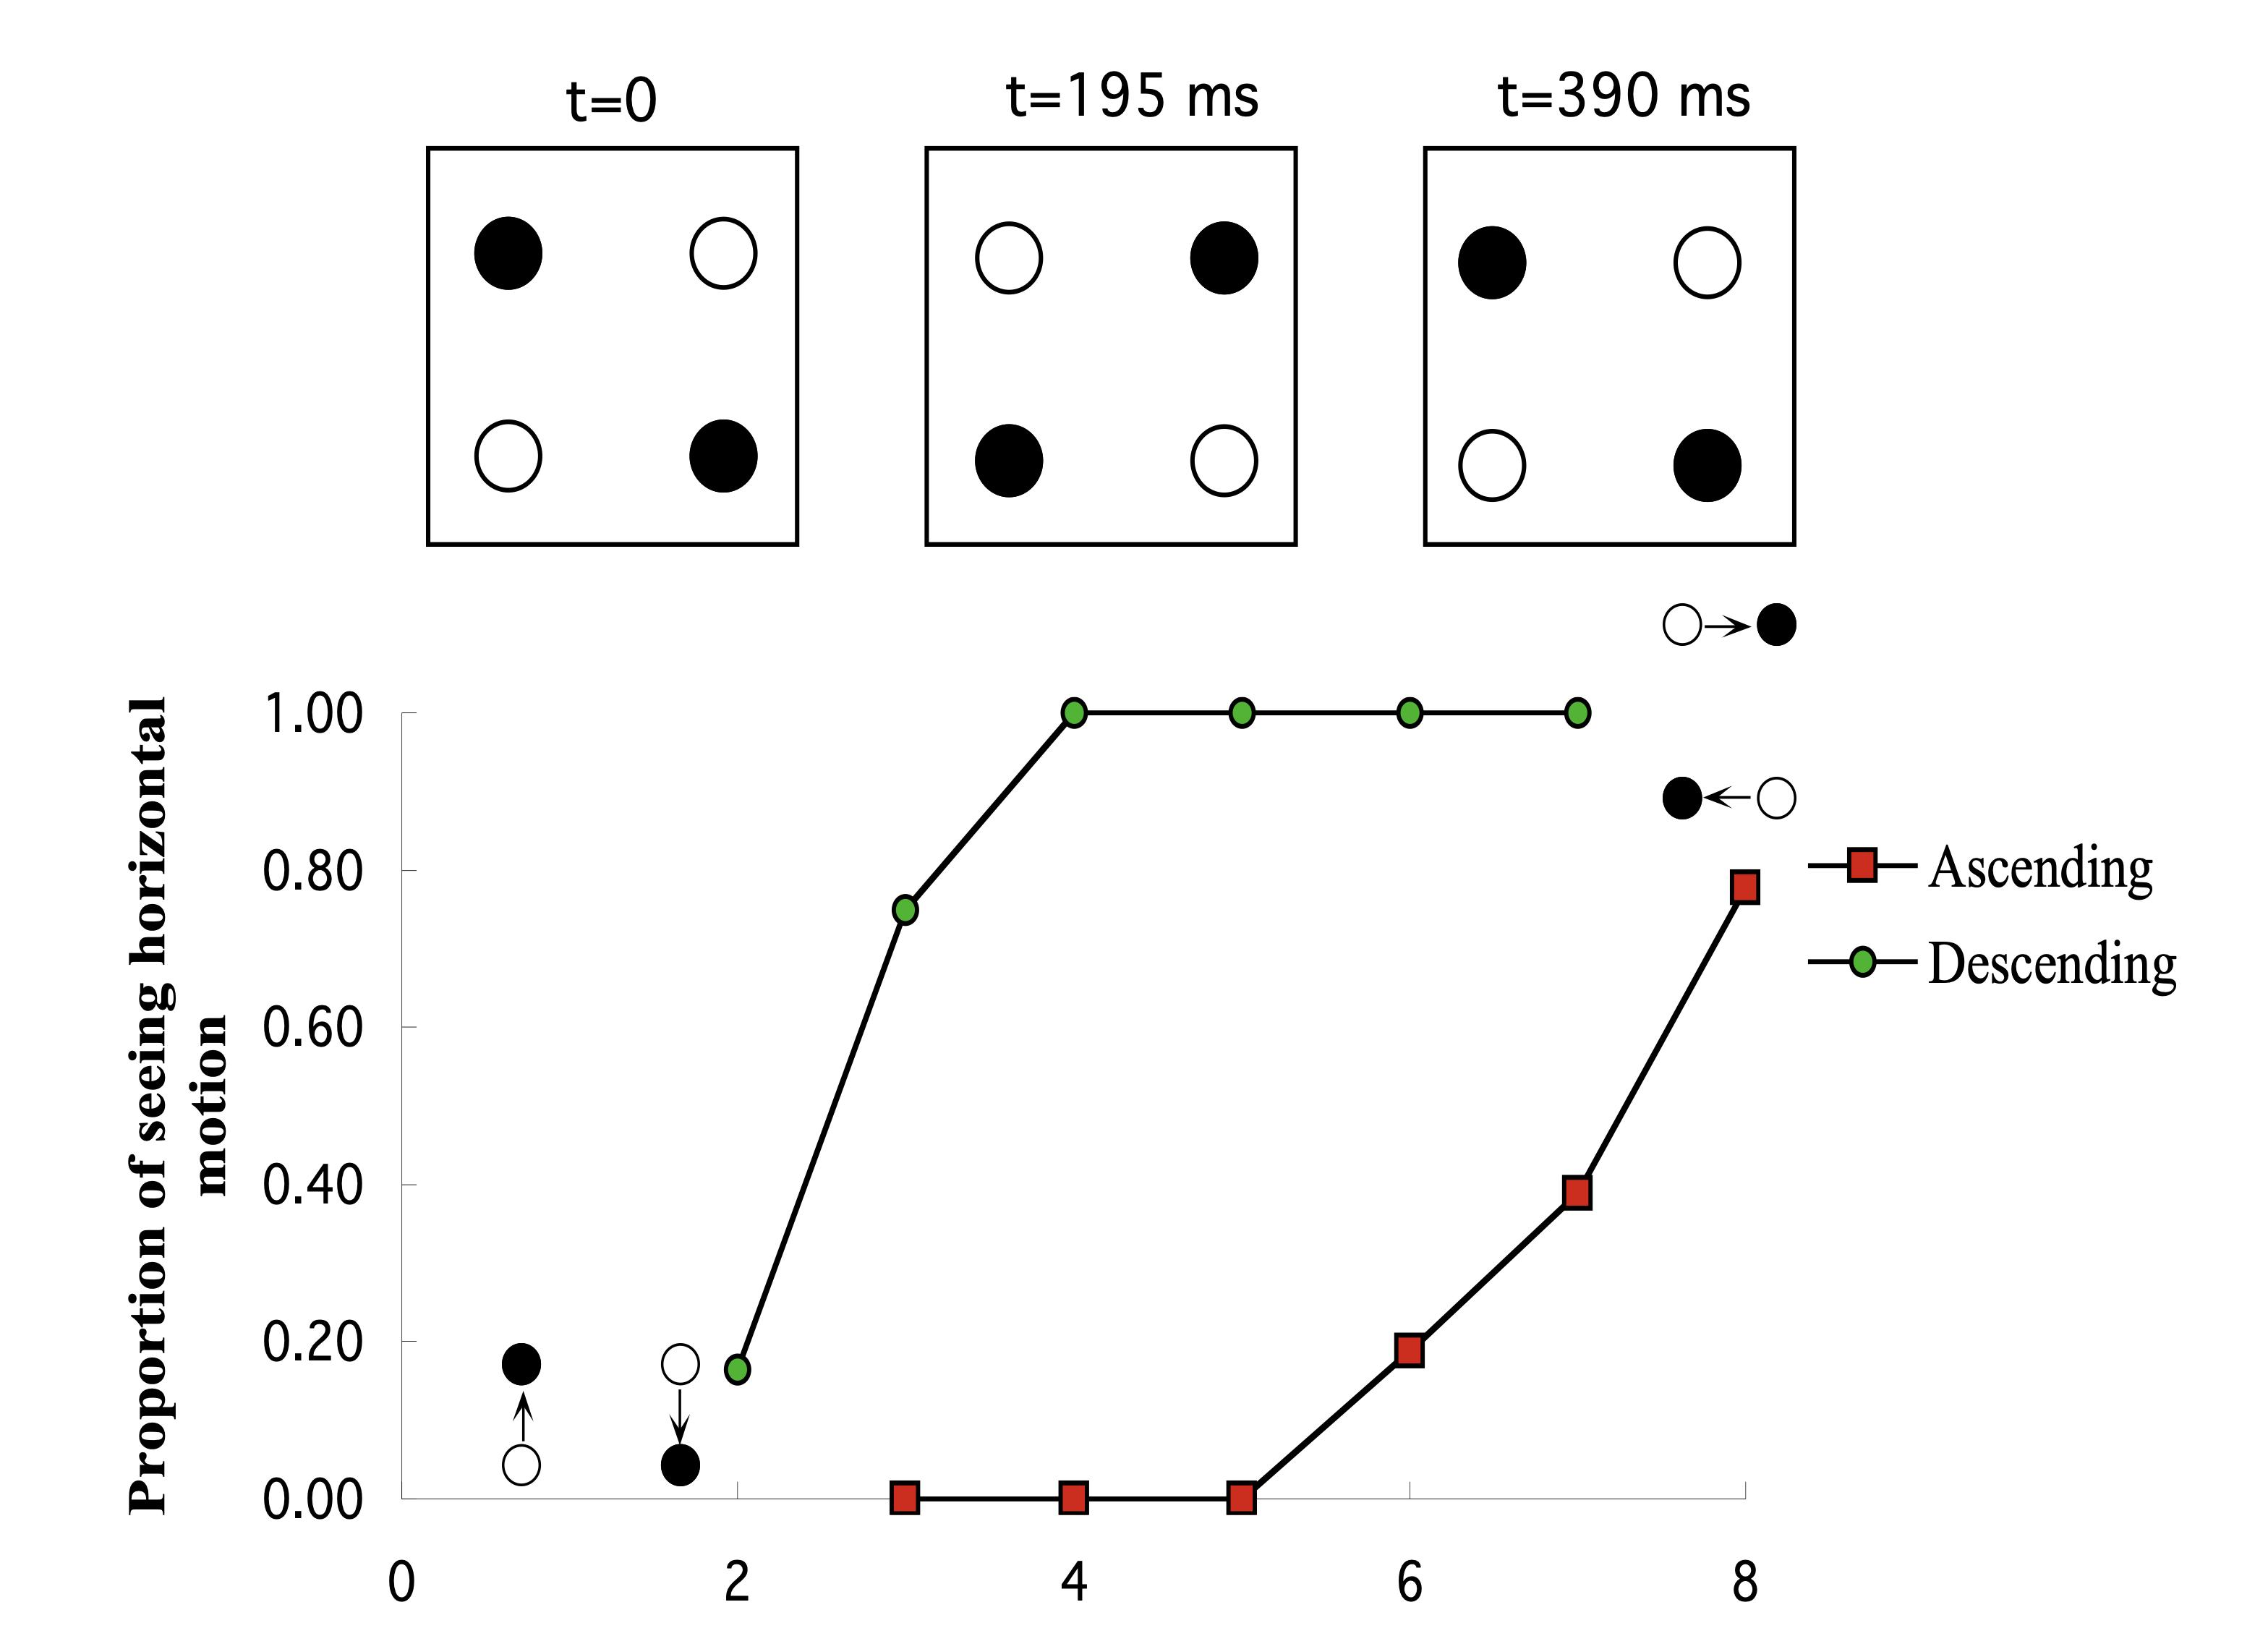
\includegraphics[width=13cm,height=\textheight]{media/ch3/image22.jpg}

}

\caption{\label{fig-ch3-img22-old-34}Hysteresis in the perception of
apparent motion. Switches between the perception of vertical or
horizontal apparent motion occur when the aspect ratio (horizontal axis)
is varied. The aspect ratio is the ratio of height to width of the
quartet. (Adapted from Ploeger, van der Maas, and Hartelman (2002) with
permission)}

\end{figure}%

\subsubsection{Anomalous variance, divergence of linear response, and
critical slowing
down}\label{sec-Anomalous-variance-divergence-of-linear-response-and-critical-slowing-down}

Gilmore's last three flags---anomalous variance, divergence of linear
response, and critical slowing down---are indicators that occur near the
bifurcation lines. They are also known as early warning signals and are
a popular topic of research (Dakos et al. 2012).
{\marginnote{\begin{footnotesize}Early warnings are indicators or
signals that precede and predict transitions within a system, allowing
for anticipation and potentially preventative
action.\end{footnotesize}}}

Anomalous variance occurs because near a bifurcation point the second
derivative diminishes, meaning that the minimum becomes less deep.
Assuming there is always some perturbation of the state, this will lead
to larger fluctuations in the state.

Divergence of linear response is the size of the effect of a small
perturbation of the state, which will be greater near a bifurcation
point. It will also take longer to return to equilibrium. This delay in
return time is known as critical slowing down and is also studied in
other approaches to nonlinear dynamical systems (e.g., synergetics,
Haken 1977). Examples of applications in psychology can be found in
Leemput et al. (2014) and Olthof et al. (2020). A somewhat critical
review is provided in Dablander et al. (2023).

In my experience, the problem with early warning signals is that both
type 1 and type 2 errors should be low for predicting transitions. This
is challenging even in simulations, let alone in noisy psychological
data. It would be fantastic if these early warnings really worked. For
example, being able to predict a relapse into depression or addiction
would be of great clinical value.

Together, the catastrophe flags provide a methodology for phase
transition research in psychology. A single flag may not be sufficient,
but the combination is. For example, the combination of evidence for
inaccessibility and hysteresis is convincing. I have given psychological
examples of most of the flags. Which flags to use in a particular case
depends on the knowledge and experimental control of the control
variables. Another approach is to fit the cusp model directly to the
data. This is the subject of the next section.

\subsection{Fitting the cusp to cross-sectional
data}\label{sec-Fitting-the-cusp-to-crosssectional-data}

\subsubsection{Cobb's maximum likelihood
approach}\label{sec-Cobbs-maximum-likelihood-approach}

In a series of papers, Loren Cobb and colleagues (Cobb and Zacks 1985;
Cobb 1978) developed a maximum likelihood approach\footnote{The is
  method finds the parameter values that make the observed data most
  probable.} to fit the cusp catastrophe to data consisting of
cross-sectional measurements of \(X\), \(a\), and \(b\). We have
implemented this approach in a cusp R package described in Grasman, van
der Maas, and Wagenmakers (2009).

The basic idea is to make catastrophe theory, a deterministic theory,
stochastic by adding a stochastic term, called Wiener noise (with
variance \(\sigma^{2})\), to equation~\ref{eq-ch3-2-old-6}\footnote{Many
  different notations exist for this. Perhaps clearer is
  \(dX(t) = - V^{'}\left( X(t) \right)dt + \sigma dW(t)\), as \(dX\) and
  \(dW\) depend on time.}:

\begin{equation}\phantomsection\label{eq-ch3-9-old-13}{
dX = - V^{'}(X)dt + \sigma dW(t).}\end{equation}

It is important to note that this type of stochasticity is not the same
as measurement noise. Measurement noise---that is, \(\varepsilon\) in
\(Y = X + \varepsilon\)---does not affect the dynamics of \(X\). Wiener
noise does; it is part of the updating equation of \(X\) itself.
{\marginnote{\begin{footnotesize}A stochastic differential equation
(SDE) is a differential equation that incorporates a term representing
random fluctuations.\end{footnotesize}}} This stochastic differential
equation is associated with a probability distribution of the form:

\begin{equation}\phantomsection\label{eq-ch3-10-old-14}{
f(X) = \frac{1}{{Z\sigma}^{2}}e^{\frac{- V(X)}{\sigma^{2}}},}\end{equation}

where \(Z\) is a normalizing constant\footnote{For consistency with
  later chapters, I define \(Z\) differently from the notation in
  Grasman, van der Maas, and Wagenmakers (2009). It is the inverse of
  \(Z\) in that paper.} necessary to ensure that the area under \(f(X)\)
is 1. This may look complicated, but for the quadratic case
\(V(X) = {\frac{1}{2}X}^{2}\), this results in the standard normal
distribution, with \(Z = {\sqrt{2\pi}}/{\sigma}\).

As in the case of the normal distribution, we want to allow for some
transformations of the variables. To simplify the necessary statistical
notation, we write the cusp as
\(V(y) = {- \alpha y - \frac{1}{2}\beta y^{2} + \frac{1}{4}y}^{4}\). The
probability distribution for the cusp is:

\begin{equation}\phantomsection\label{eq-ch3-11-old-15}{
f(y) = \frac{1}{{Z\sigma}^{2}}e^{\frac{\alpha y + \frac{1}{2}\beta y^{2} - \frac{1}{4}y^{4}}{\sigma^{2}}}.}\end{equation}

As in regression models, the cusp variables are modeled as linear
function of measured variables. That is, the dependent variables
\(Y_{i1},\ Y_{i2},\ldots,Y_{ip}\) and the independent variables
\(X_{i1},\ X_{i2},\ldots,X_{iq}\), for subjects \(i = 1,\ldots,n\), are
related to the cusp variables as follows:

\begin{equation}\phantomsection\label{eq-ch3-12-old-16}{
\begin{gathered}
y_{i} = w_{0} + w_{1}Y_{i1} + w_{2}Y_{i2} + \ldots + w_{p}Y_{ip} \\
\alpha_{i} = a_{0} + a_{1}X_{i1} + a_{2}X_{i2} + \ldots + a_{q}X_{iq} \\
\beta_{i} = b_{0} + b_{1}X_{i1} + b_{2}X_{i2} + \ldots + b_{q}X_{iq}
\end{gathered}
}\end{equation}

By estimating these regression parameters, we fit the cusp model to
empirical data. The cusp package in R makes this possible. I will first
demonstrate this using simulated data.
{\marginnote{\begin{footnotesize}My number-one rule when using
statistical techniques: Never use a statistical technique on real data
before you have tested it on simulated data.\end{footnotesize}}} I
strongly recommend this approach. First, it forces you to understand
what the statistical technique actually does, and second, it gives you a
way to test the power and investigate violations of the technique's
assumptions.

\begin{Shaded}
\begin{Highlighting}[]
\FunctionTok{library}\NormalTok{(cusp) }\CommentTok{\# if error: install.packages(\textquotesingle{}cusp\textquotesingle{})}
\FunctionTok{set.seed}\NormalTok{(}\DecValTok{1}\NormalTok{)}
\NormalTok{X1 }\OtherTok{\textless{}{-}} \FunctionTok{runif}\NormalTok{(}\DecValTok{1000}\NormalTok{) }\CommentTok{\# independent variable 1}
\NormalTok{X2 }\OtherTok{\textless{}{-}} \FunctionTok{runif}\NormalTok{(}\DecValTok{1000}\NormalTok{) }\CommentTok{\# independent variable 2}
\CommentTok{\# to be estimated parameters}
\NormalTok{w0 }\OtherTok{\textless{}{-}} \DecValTok{2}\NormalTok{; w1 }\OtherTok{\textless{}{-}} \DecValTok{4}\NormalTok{; a0 }\OtherTok{\textless{}{-}} \SpecialCharTok{{-}}\DecValTok{2}\NormalTok{; a1 }\OtherTok{\textless{}{-}} \DecValTok{3}\NormalTok{; b0 }\OtherTok{\textless{}{-}} \SpecialCharTok{{-}}\DecValTok{2}\NormalTok{; b1 }\OtherTok{\textless{}{-}} \DecValTok{4} 
\CommentTok{\# sample Y1 according to cusp using rcusp and the chosen parameter values}
\NormalTok{Y1 }\OtherTok{\textless{}{-}} \SpecialCharTok{{-}}\NormalTok{w0}\SpecialCharTok{/}\NormalTok{w1 }\SpecialCharTok{+}\NormalTok{ (}\DecValTok{1}\SpecialCharTok{/}\NormalTok{w1) }\SpecialCharTok{*} \FunctionTok{Vectorize}\NormalTok{(rcusp)(}\DecValTok{1}\NormalTok{, a0}\SpecialCharTok{+}\NormalTok{a1}\SpecialCharTok{*}\NormalTok{X1, b0}\SpecialCharTok{+}\NormalTok{b1}\SpecialCharTok{*}\NormalTok{X2) }
\NormalTok{data }\OtherTok{\textless{}{-}} \FunctionTok{data.frame}\NormalTok{(X1, X2, Y1) }\CommentTok{\# collect ‘measured’ variables in data}
\end{Highlighting}
\end{Shaded}

I recommend doing some descriptive analysis first. With
\texttt{hist(data\$Y1)} we can inspect whether there is some indication
of bimodality. \(X2\) is the splitting variable, so perhaps we see
stronger bimodality with
\texttt{hist(data\$Y1{[}data\$X2\textgreater{}mean(data\$X2){]}}). The
function pairs in R, \texttt{pairs(data)}, is also always recommended.
In this perfect simulated case, you will already see strong indications
of the cusp. Now we fit the full model with \(\alpha\) and \(\beta\)
both as function of \(X1\) and \(X2\).

\begin{Shaded}
\begin{Highlighting}[]
\NormalTok{fit }\OtherTok{\textless{}{-}} \FunctionTok{cusp}\NormalTok{(y }\SpecialCharTok{\textasciitilde{}}\NormalTok{ Y1, alpha }\SpecialCharTok{\textasciitilde{}}\NormalTok{ X1}\SpecialCharTok{+}\NormalTok{X2, beta }\SpecialCharTok{\textasciitilde{}}\NormalTok{ X1}\SpecialCharTok{+}\NormalTok{X2, data) }
\FunctionTok{summary}\NormalTok{(fit) }
\end{Highlighting}
\end{Shaded}

The table provides a summary:

\begin{longtable}[]{@{}
  >{\raggedright\arraybackslash}p{(\columnwidth - 8\tabcolsep) * \real{0.2687}}
  >{\centering\arraybackslash}p{(\columnwidth - 8\tabcolsep) * \real{0.1493}}
  >{\centering\arraybackslash}p{(\columnwidth - 8\tabcolsep) * \real{0.1791}}
  >{\centering\arraybackslash}p{(\columnwidth - 8\tabcolsep) * \real{0.1343}}
  >{\centering\arraybackslash}p{(\columnwidth - 8\tabcolsep) * \real{0.2687}}@{}}
\caption{Table 3.1: The parameter estimates including standard errors
and p-values generated by the cusp package.}\tabularnewline
\toprule\noalign{}
\begin{minipage}[b]{\linewidth}\raggedright
Coefficients
\end{minipage} & \begin{minipage}[b]{\linewidth}\centering
Estimate
\end{minipage} & \begin{minipage}[b]{\linewidth}\centering
Std. Error
\end{minipage} & \begin{minipage}[b]{\linewidth}\centering
z-value
\end{minipage} & \begin{minipage}[b]{\linewidth}\centering
Pr(\textgreater\textbar z\textbar)
\end{minipage} \\
\midrule\noalign{}
\endfirsthead
\toprule\noalign{}
\begin{minipage}[b]{\linewidth}\raggedright
Coefficients
\end{minipage} & \begin{minipage}[b]{\linewidth}\centering
Estimate
\end{minipage} & \begin{minipage}[b]{\linewidth}\centering
Std. Error
\end{minipage} & \begin{minipage}[b]{\linewidth}\centering
z-value
\end{minipage} & \begin{minipage}[b]{\linewidth}\centering
Pr(\textgreater\textbar z\textbar)
\end{minipage} \\
\midrule\noalign{}
\endhead
\bottomrule\noalign{}
\endlastfoot
a{[}(Intercept){]} & -2.13 & 0.19 & -11.0 & \textless{}
2e-16\textsuperscript{***} \\
a{[}X1{]} & 3.11 & 0.22 & 14.2 & \textless{}
2e-16\textsuperscript{***} \\
a{[}X2{]} & 0.15 & 0.17 & 0.9 & 0.39 \\
b{[}(Intercept){]} & -2.29 & 0.34 & -6.7 &
2.66e-11\textsuperscript{***} \\
b{[}X1{]} & -0.09 & 0.33 & -0.3 & 0.79 \\
b{[}X2{]} & 4.40 & 0.27 & 16.5 & \textless{}
2e-16\textsuperscript{***} \\
w{[}(Intercept){]} & 1.98 & 0.07 & 27.6 & \textless{}
2e-16\textsuperscript{***} \\
w{[}Y1{]} & 3.97 & 0.10 & 38.0 & \textless{}
2e-16\textsuperscript{***} \\
\end{longtable}

Note that we fit a model with too many parameters. We also estimated
\(a_{2}\) and \(b_{1}\) (because the model was specified as alpha
\textasciitilde{} \$X\(1+\)X\$2, beta \textasciitilde{} \$X\(1+\)X\$2).
These estimates are not significantly different from 0. The other
parameters are estimated reasonably close to their true values, since
the true values fall within the confidence interval of the estimates
(defined by twice the standard error on either side). We expect a better
fit in terms of AIC and BIC when we fit a reduced model without
\(a_{2}\) and \(b_{1}\). These fit indices penalize the goodness of fit
(e.g., the log-likelihood) for the number of parameters used to
discourage overfitting and to promote model parsimony.

\begin{Shaded}
\begin{Highlighting}[]
\NormalTok{fit\_correct\_model }\OtherTok{\textless{}{-}} \FunctionTok{cusp}\NormalTok{(y }\SpecialCharTok{\textasciitilde{}}\NormalTok{ Y1, alpha }\SpecialCharTok{\textasciitilde{}}\NormalTok{ X1, beta }\SpecialCharTok{\textasciitilde{}}\NormalTok{ X2, data) }
\FunctionTok{summary}\NormalTok{(fit\_correct\_model)}
\end{Highlighting}
\end{Shaded}

\begin{longtable}[]{@{}
  >{\raggedright\arraybackslash}p{(\columnwidth - 12\tabcolsep) * \real{0.2308}}
  >{\centering\arraybackslash}p{(\columnwidth - 12\tabcolsep) * \real{0.1692}}
  >{\centering\arraybackslash}p{(\columnwidth - 12\tabcolsep) * \real{0.1385}}
  >{\centering\arraybackslash}p{(\columnwidth - 12\tabcolsep) * \real{0.0923}}
  >{\centering\arraybackslash}p{(\columnwidth - 12\tabcolsep) * \real{0.1231}}
  >{\centering\arraybackslash}p{(\columnwidth - 12\tabcolsep) * \real{0.1231}}
  >{\centering\arraybackslash}p{(\columnwidth - 12\tabcolsep) * \real{0.1231}}@{}}
\caption{Table 3.2: The comparative fit measures AIC, AICc, and BIC
indicate that the reduced model should be the model of
choice.}\tabularnewline
\toprule\noalign{}
\begin{minipage}[b]{\linewidth}\raggedright
\end{minipage} & \begin{minipage}[b]{\linewidth}\centering
R.Squared
\end{minipage} & \begin{minipage}[b]{\linewidth}\centering
logLik
\end{minipage} & \begin{minipage}[b]{\linewidth}\centering
npar
\end{minipage} & \begin{minipage}[b]{\linewidth}\centering
AIC
\end{minipage} & \begin{minipage}[b]{\linewidth}\centering
AICc
\end{minipage} & \begin{minipage}[b]{\linewidth}\centering
BIC
\end{minipage} \\
\midrule\noalign{}
\endfirsthead
\toprule\noalign{}
\begin{minipage}[b]{\linewidth}\raggedright
\end{minipage} & \begin{minipage}[b]{\linewidth}\centering
R.Squared
\end{minipage} & \begin{minipage}[b]{\linewidth}\centering
logLik
\end{minipage} & \begin{minipage}[b]{\linewidth}\centering
npar
\end{minipage} & \begin{minipage}[b]{\linewidth}\centering
AIC
\end{minipage} & \begin{minipage}[b]{\linewidth}\centering
AICc
\end{minipage} & \begin{minipage}[b]{\linewidth}\centering
BIC
\end{minipage} \\
\midrule\noalign{}
\endhead
\bottomrule\noalign{}
\endlastfoot
Full model & 0.428 & -1058.7 & 8 & 2133.3 & 2133.5 & 2172.6 \\
Reduced model & 0.426 & -1059.0 & 6 & 2130.0 & 2130.1 & 2159.5 \\
\end{longtable}

The next simulation demonstrates that we can detect hysteresis using
this approach. We simulate data with \(- 2 < \alpha < 2,\) and fixed
\(\beta\). If \(\beta < 0\) we have no hysteresis, but if \(\beta > 0\),
we do have hysteresis. With the code below we simulate datasets for
different \(\beta\) and compare the goodness of fit between the linear
and cusp model. Figure~\ref{fig-ch3-img23-old-35} summarizes the
results. Note that a lower BIC indicated the better-fitting model.

\begin{Shaded}
\begin{Highlighting}[]
\FunctionTok{set.seed}\NormalTok{(}\DecValTok{10}\NormalTok{)}
\NormalTok{n }\OtherTok{\textless{}{-}} \DecValTok{500}
\NormalTok{X1 }\OtherTok{\textless{}{-}} \FunctionTok{seq}\NormalTok{(}\SpecialCharTok{{-}}\DecValTok{1}\NormalTok{,}\DecValTok{1}\NormalTok{,}\AttributeTok{le=}\NormalTok{n) }\CommentTok{\# rnorm(n) \#runif(1000) \# independent variable 1}
\NormalTok{a0 }\OtherTok{\textless{}{-}} \DecValTok{0}\NormalTok{; a1 }\OtherTok{\textless{}{-}} \DecValTok{2}\NormalTok{; b0 }\OtherTok{\textless{}{-}} \DecValTok{2} \CommentTok{\# to be estimated parameters}
\NormalTok{b0s }\OtherTok{\textless{}{-}} \FunctionTok{seq}\NormalTok{(}\SpecialCharTok{{-}}\DecValTok{1}\NormalTok{,}\DecValTok{2}\NormalTok{,}\AttributeTok{by=}\NormalTok{.}\DecValTok{25}\NormalTok{)}
\NormalTok{i }\OtherTok{\textless{}{-}} \DecValTok{0}
\NormalTok{dat }\OtherTok{\textless{}{-}} \FunctionTok{matrix}\NormalTok{(}\DecValTok{0}\NormalTok{,}\FunctionTok{length}\NormalTok{(b0s),}\DecValTok{7}\NormalTok{)}
\ControlFlowTok{for}\NormalTok{ (b0 }\ControlFlowTok{in}\NormalTok{ b0s)}
\NormalTok{\{}
\NormalTok{  i }\OtherTok{\textless{}{-}}\NormalTok{ i }\SpecialCharTok{+} \DecValTok{1}
\NormalTok{  Y1 }\OtherTok{\textless{}{-}} \FunctionTok{Vectorize}\NormalTok{(rcusp)(}\DecValTok{1}\NormalTok{, a1 }\SpecialCharTok{*}\NormalTok{ X1, b0)}
\NormalTok{  data }\OtherTok{\textless{}{-}} \FunctionTok{data.frame}\NormalTok{(X1, Y1) }\CommentTok{\# collect ‘measured’ variables in data}
\NormalTok{  fit }\OtherTok{\textless{}{-}} \FunctionTok{cusp}\NormalTok{(y }\SpecialCharTok{\textasciitilde{}}\NormalTok{ Y1, alpha }\SpecialCharTok{\textasciitilde{}}\NormalTok{ X1, beta }\SpecialCharTok{\textasciitilde{}} \DecValTok{1}\NormalTok{, data)}
\NormalTok{  sf }\OtherTok{\textless{}{-}} \FunctionTok{summary}\NormalTok{(fit)}
\NormalTok{  dat[i, ] }\OtherTok{\textless{}{-}} \FunctionTok{c}\NormalTok{(b0, sf}\SpecialCharTok{$}\NormalTok{r2lin.r.squared[}\DecValTok{1}\NormalTok{], sf}\SpecialCharTok{$}\NormalTok{r2cusp.r.squared[}\DecValTok{1}\NormalTok{],}
\NormalTok{                sf}\SpecialCharTok{$}\NormalTok{r2lin.bic[}\DecValTok{1}\NormalTok{],sf}\SpecialCharTok{$}\NormalTok{r2cusp.bic[}\DecValTok{1}\NormalTok{],}
\NormalTok{                sf}\SpecialCharTok{$}\NormalTok{r2lin.aic[}\DecValTok{1}\NormalTok{], sf}\SpecialCharTok{$}\NormalTok{r2cusp.aic[}\DecValTok{1}\NormalTok{])}
\NormalTok{\}}
\FunctionTok{par}\NormalTok{(}\AttributeTok{mar=}\FunctionTok{c}\NormalTok{(}\DecValTok{4}\NormalTok{,}\DecValTok{5}\NormalTok{,}\DecValTok{1}\NormalTok{,}\DecValTok{1}\NormalTok{))}
\FunctionTok{matplot}\NormalTok{(dat[,}\DecValTok{1}\NormalTok{],dat[,}\DecValTok{4}\SpecialCharTok{:}\DecValTok{5}\NormalTok{],}\AttributeTok{ylab=}\StringTok{\textquotesingle{}Bic\textquotesingle{}}\NormalTok{,}\AttributeTok{xlab=}\StringTok{\textquotesingle{}b0\textquotesingle{}}\NormalTok{,}\AttributeTok{bty=}\StringTok{\textquotesingle{}n\textquotesingle{}}\NormalTok{,}\AttributeTok{type=}\StringTok{\textquotesingle{}b\textquotesingle{}}\NormalTok{,}
        \AttributeTok{pch=}\DecValTok{1}\SpecialCharTok{:}\DecValTok{2}\NormalTok{,}\AttributeTok{cex.lab=}\FloatTok{1.5}\NormalTok{)}
\FunctionTok{legend}\NormalTok{(}\StringTok{\textquotesingle{}right\textquotesingle{}}\NormalTok{,}\AttributeTok{legend=}\FunctionTok{c}\NormalTok{(}\StringTok{\textquotesingle{}linear\textquotesingle{}}\NormalTok{,}\StringTok{\textquotesingle{}cusp\textquotesingle{}}\NormalTok{),}\AttributeTok{lty=}\DecValTok{1}\SpecialCharTok{:}\DecValTok{2}\NormalTok{,}\AttributeTok{pch=}\DecValTok{1}\SpecialCharTok{:}\DecValTok{2}\NormalTok{,}
       \AttributeTok{col=}\DecValTok{1}\SpecialCharTok{:}\DecValTok{2}\NormalTok{,}\AttributeTok{cex=}\FloatTok{1.5}\NormalTok{)}
\FunctionTok{abline}\NormalTok{(}\AttributeTok{v=}\DecValTok{0}\NormalTok{,}\AttributeTok{lty=}\DecValTok{3}\NormalTok{)}
\FunctionTok{text}\NormalTok{(}\SpecialCharTok{{-}}\NormalTok{.}\DecValTok{5}\NormalTok{,}\DecValTok{800}\NormalTok{, }\StringTok{\textquotesingle{}no hysteresis\textquotesingle{}}\NormalTok{,}\AttributeTok{cex=}\FloatTok{1.5}\NormalTok{)}
\FunctionTok{text}\NormalTok{(.}\DecValTok{5}\NormalTok{,}\DecValTok{800}\NormalTok{, }\StringTok{\textquotesingle{}hysteresis\textquotesingle{}}\NormalTok{,}\AttributeTok{cex=}\FloatTok{1.5}\NormalTok{)}
\end{Highlighting}
\end{Shaded}

\begin{figure}

\centering{

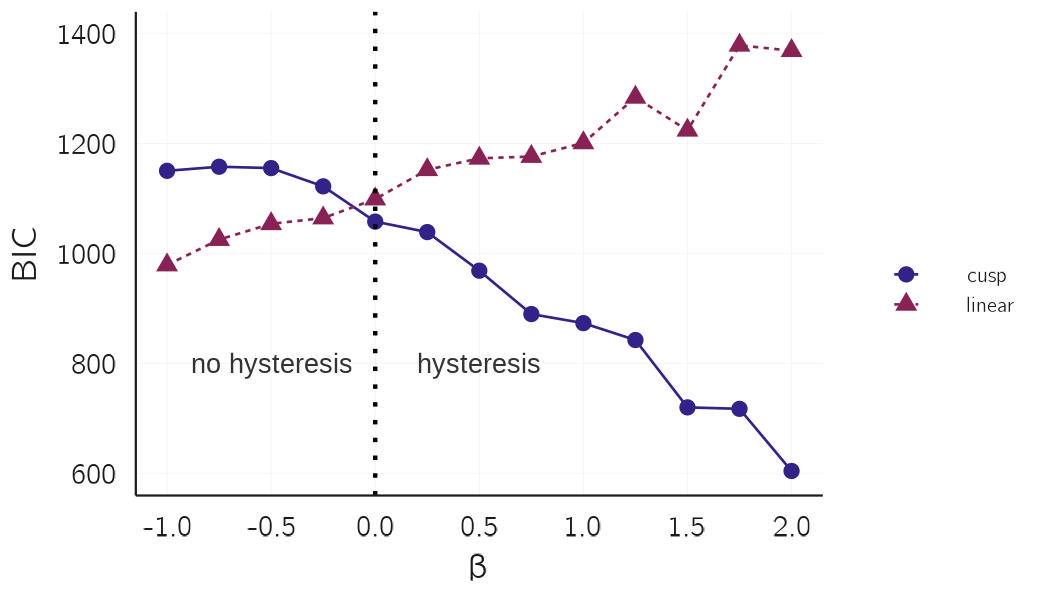
\includegraphics[width=8.33333in,height=\textheight]{media/ch3/fig-ch3-img23-old-35.jpg}

}

\caption{\label{fig-ch3-img23-old-35}At the back of the cusp (low
\(b_0\)), the cusp is approximately linear, the BIC favors this simpler
model (dotted line) over the cusp mode (solid line).}

\end{figure}%

\subsubsection{Empirical examples}\label{sec-Empirical-examples}

In Grasman, van der Maas, and Wagenmakers (2009), we present several
examples with real data. As another example, we use Stoufer's data,
which we used as an example of divergence before (see
figure~\ref{fig-ch3-img21-old-33}).

\begin{Shaded}
\begin{Highlighting}[]
\NormalTok{x }\OtherTok{\textless{}{-}} \FunctionTok{read.table}\NormalTok{(}\StringTok{\textquotesingle{}data/stoufer.txt\textquotesingle{}}\NormalTok{)}
\FunctionTok{colnames}\NormalTok{(x) }\OtherTok{\textless{}{-}} \FunctionTok{c}\NormalTok{(}\StringTok{\textquotesingle{}IntensityofFeeling\textquotesingle{}}\NormalTok{,}\StringTok{\textquotesingle{}Attitude\textquotesingle{}}\NormalTok{)}
\NormalTok{fit }\OtherTok{\textless{}{-}} \FunctionTok{cusp}\NormalTok{(y }\SpecialCharTok{\textasciitilde{}}\NormalTok{ Attitude, alpha }\SpecialCharTok{\textasciitilde{}}\NormalTok{ IntensityofFeeling, }
\NormalTok{            beta }\SpecialCharTok{\textasciitilde{}}\NormalTok{ IntensityofFeeling, x)}
\FunctionTok{summary}\NormalTok{(fit)}
\end{Highlighting}
\end{Shaded}

Inspection of the parameter estimates shows that, as expected, intensity
of feeling only loads on the splitting axis and not on the normal axis.
Figure~\ref{fig-ch3-img24-old-36} shows the location of the data in the
bifurcation set (\texttt{plot(fit)}).

\begin{figure}

\centering{

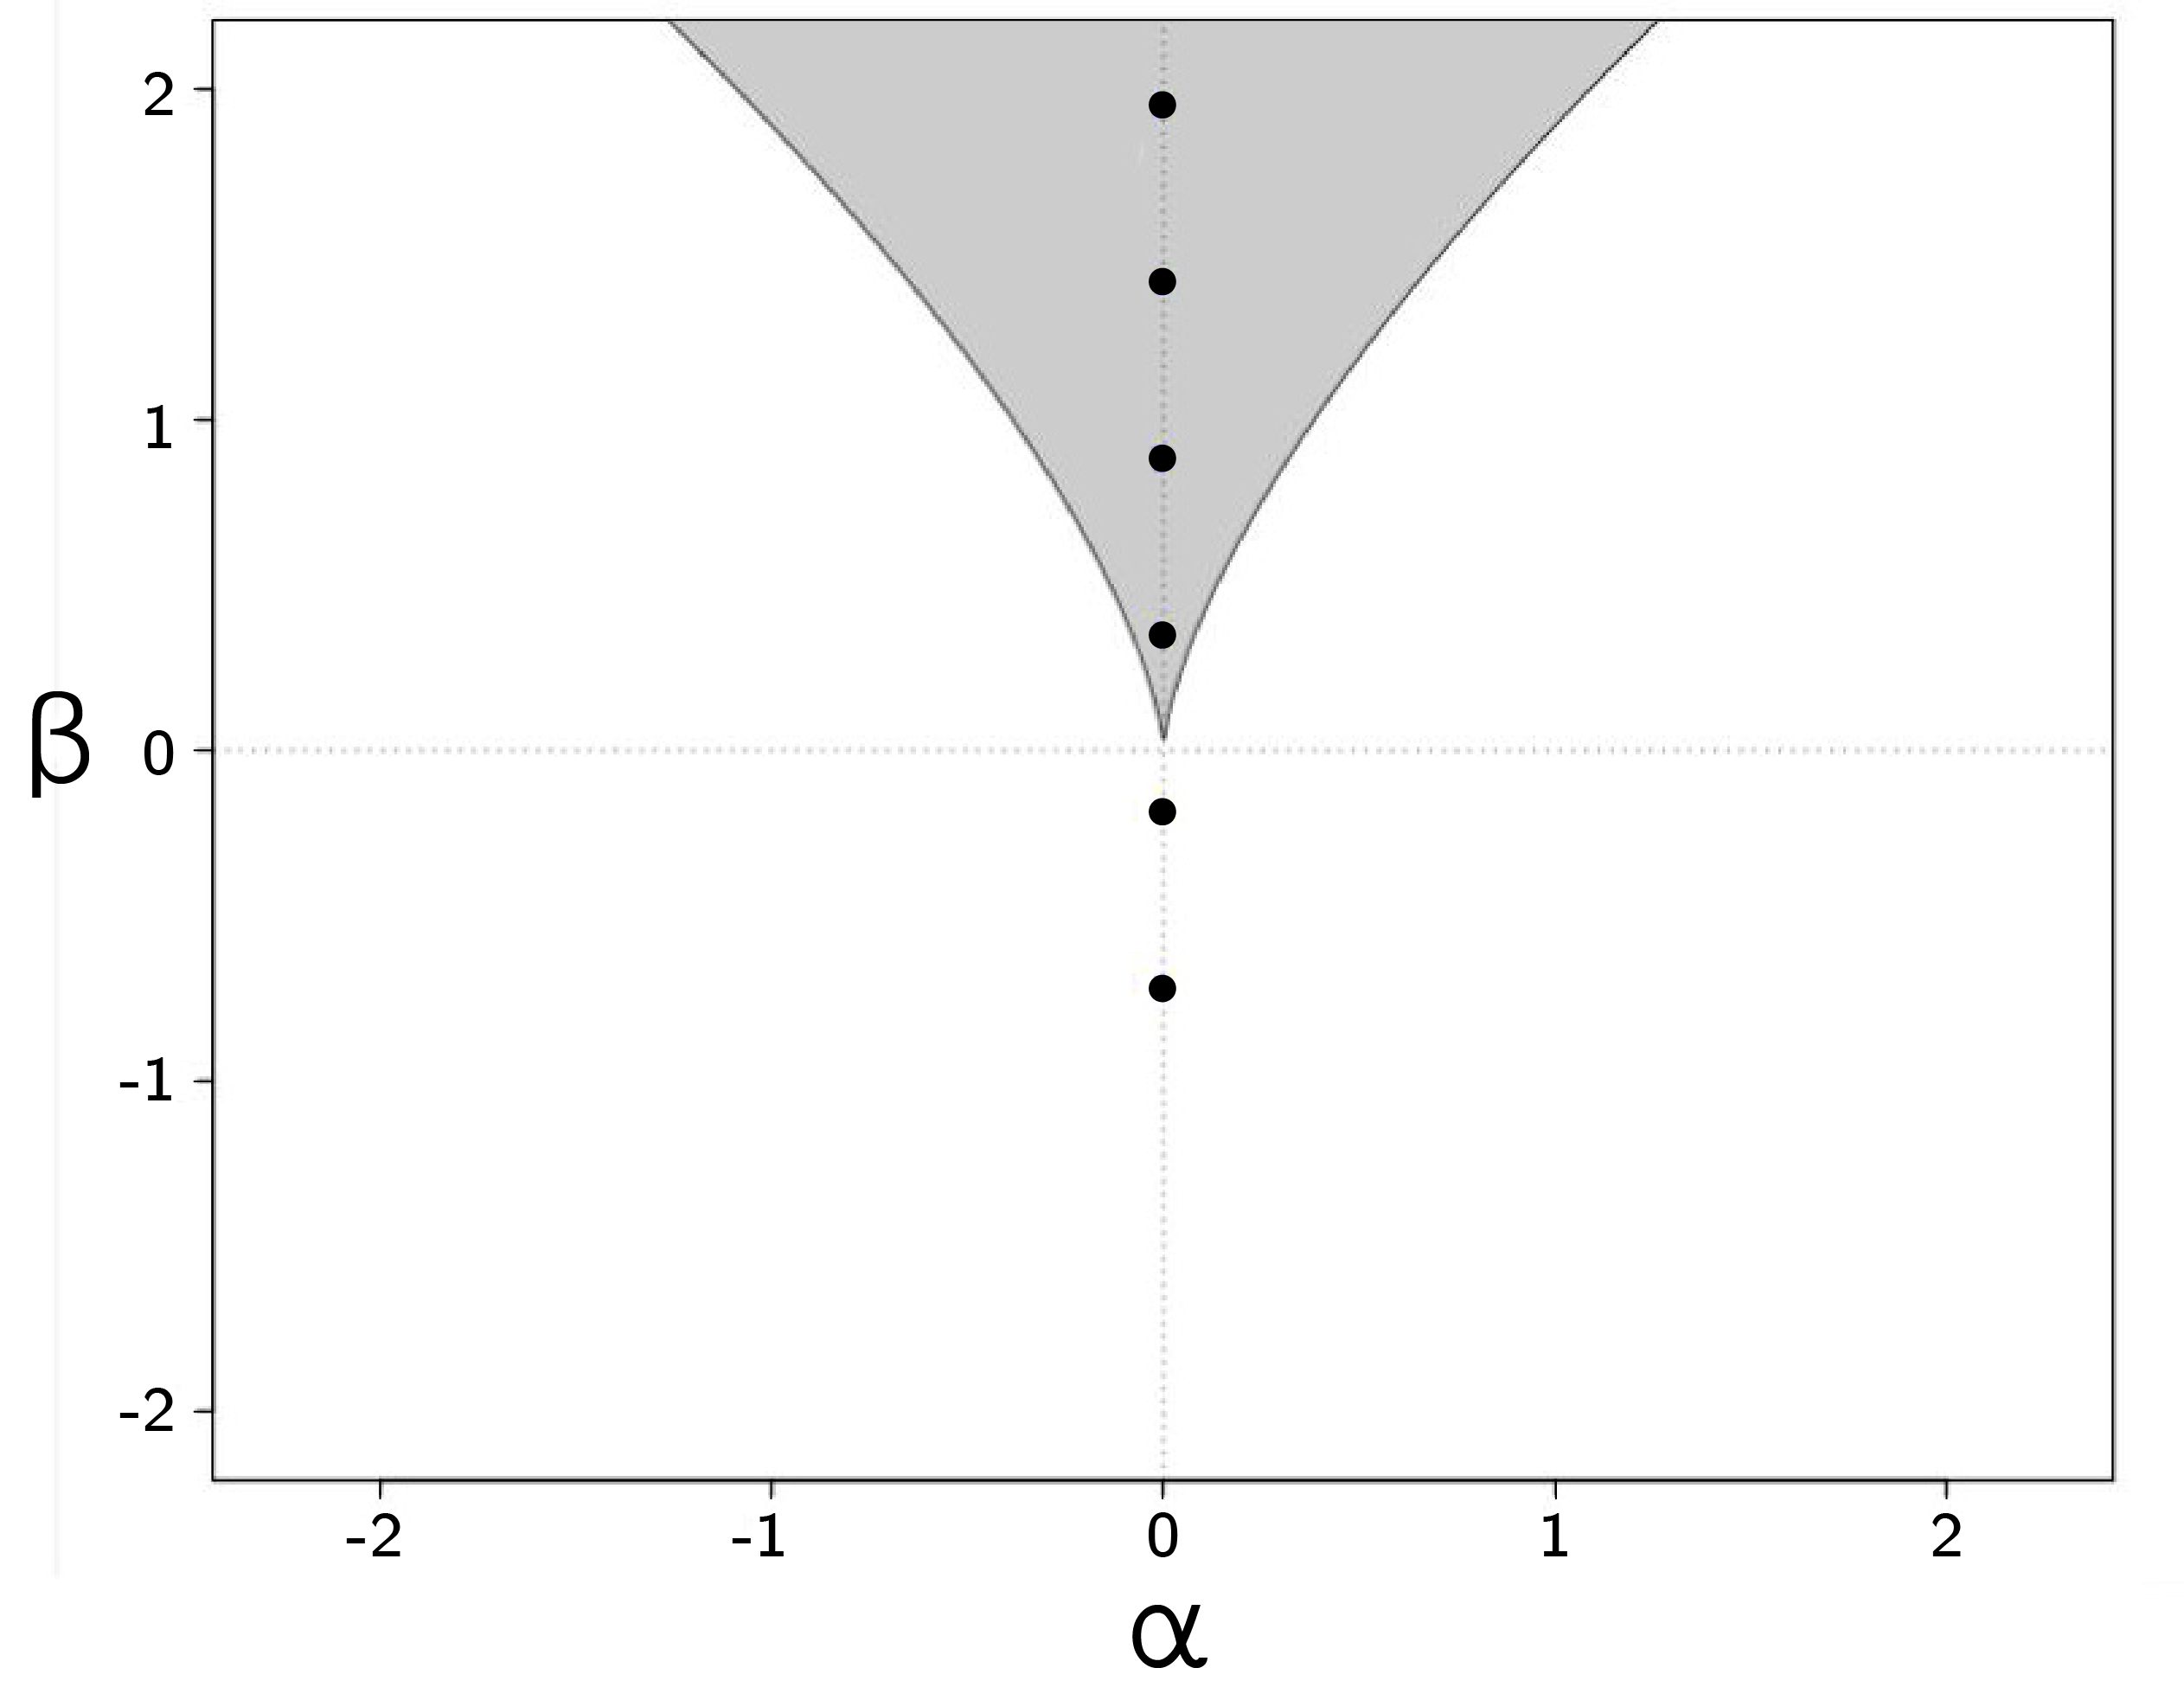
\includegraphics{media/ch3/ch3-24__figure36.png}

}

\caption{\label{fig-ch3-img24-old-36}Placement of the data of
figure~\ref{fig-ch3-img21-old-33} in the bifurcation set.}

\end{figure}%

Another example is the conservation dataset of Bentler (1970), which
contains the scores on a 12-item test from a conservation test of 560
children from eight different age groups
(figure~\ref{fig-ch3-img25-old-37}). These data are expected to be
bimodal and to move along the normal axis (van der Maas and Molenaar
1992).

\begin{Shaded}
\begin{Highlighting}[]
\NormalTok{x }\OtherTok{\textless{}{-}} \FunctionTok{read.table}\NormalTok{(}\StringTok{\textquotesingle{}data/bentler.txt\textquotesingle{}}\NormalTok{,}\AttributeTok{header=}\NormalTok{T)}
\FunctionTok{layout}\NormalTok{(}\FunctionTok{t}\NormalTok{(}\DecValTok{1}\SpecialCharTok{:}\DecValTok{8}\NormalTok{))}
\NormalTok{age }\OtherTok{\textless{}{-}} \FunctionTok{c}\NormalTok{(}\StringTok{\textquotesingle{}age 4 to 4.5\textquotesingle{}}\NormalTok{,}\StringTok{\textquotesingle{}age 4.5 to 5\textquotesingle{}}\NormalTok{,}\StringTok{\textquotesingle{}age 5 to 5.5\textquotesingle{}}\NormalTok{,}\StringTok{\textquotesingle{}age 5.5 to 6\textquotesingle{}}\NormalTok{,}
         \StringTok{\textquotesingle{}age 6 to 6.5\textquotesingle{}}\NormalTok{,}\StringTok{\textquotesingle{}age 6.5 to 7\textquotesingle{}}\NormalTok{,}\StringTok{\textquotesingle{}age 7 to 7.5\textquotesingle{}}\NormalTok{,}\StringTok{\textquotesingle{}age 7.5 to 8\textquotesingle{}}\NormalTok{)}
\ControlFlowTok{for}\NormalTok{(i }\ControlFlowTok{in} \DecValTok{1}\SpecialCharTok{:}\DecValTok{8}\NormalTok{)}
\NormalTok{\{}
  \ControlFlowTok{if}\NormalTok{(i}\SpecialCharTok{==}\DecValTok{1}\NormalTok{) \{}\FunctionTok{par}\NormalTok{(}\AttributeTok{mar=}\FunctionTok{c}\NormalTok{(}\DecValTok{4}\NormalTok{,}\DecValTok{3}\NormalTok{,}\DecValTok{2}\NormalTok{,}\DecValTok{1}\NormalTok{));names}\OtherTok{=}\DecValTok{0}\SpecialCharTok{:}\DecValTok{12}\NormalTok{\} }\ControlFlowTok{else} 
\NormalTok{    \{names}\OtherTok{=}\StringTok{\textquotesingle{}\textquotesingle{}}\NormalTok{;}\FunctionTok{par}\NormalTok{(}\AttributeTok{mar=}\FunctionTok{c}\NormalTok{(}\DecValTok{4}\NormalTok{,}\DecValTok{1}\NormalTok{,}\DecValTok{2}\NormalTok{,}\DecValTok{1}\NormalTok{))\}}
  \FunctionTok{barplot}\NormalTok{(}\FunctionTok{table}\NormalTok{(}\FunctionTok{factor}\NormalTok{(x[x[,}\DecValTok{1}\NormalTok{]}\SpecialCharTok{==}\NormalTok{i,}\DecValTok{2}\NormalTok{],}\AttributeTok{levels=}\DecValTok{0}\SpecialCharTok{:}\DecValTok{12}\NormalTok{)),}\AttributeTok{horiz=}\NormalTok{T,}\AttributeTok{axes=}\NormalTok{F,}
          \AttributeTok{main=}\NormalTok{age[i],}\AttributeTok{xlab=}\StringTok{\textquotesingle{}\textquotesingle{}}\NormalTok{,}
          \AttributeTok{names=}\NormalTok{names,}\AttributeTok{cex.main=}\FloatTok{1.5}\NormalTok{,}\AttributeTok{cex.names=}\FloatTok{1.5}\NormalTok{)}
\NormalTok{\}}
\NormalTok{fit }\OtherTok{\textless{}{-}} \FunctionTok{cusp}\NormalTok{(y }\SpecialCharTok{\textasciitilde{}}\NormalTok{ score, alpha }\SpecialCharTok{\textasciitilde{}}\NormalTok{ age\_range, beta }\SpecialCharTok{\textasciitilde{}}\NormalTok{ age\_range, x)}
\FunctionTok{summary}\NormalTok{(fit)}
\FunctionTok{plot}\NormalTok{(fit)}
\end{Highlighting}
\end{Shaded}

This is supported by results of the cusp fit. You can verify that a
model with beta \textasciitilde{} 1 fits better according to the AIC and
BIC.

\begin{figure}

\centering{

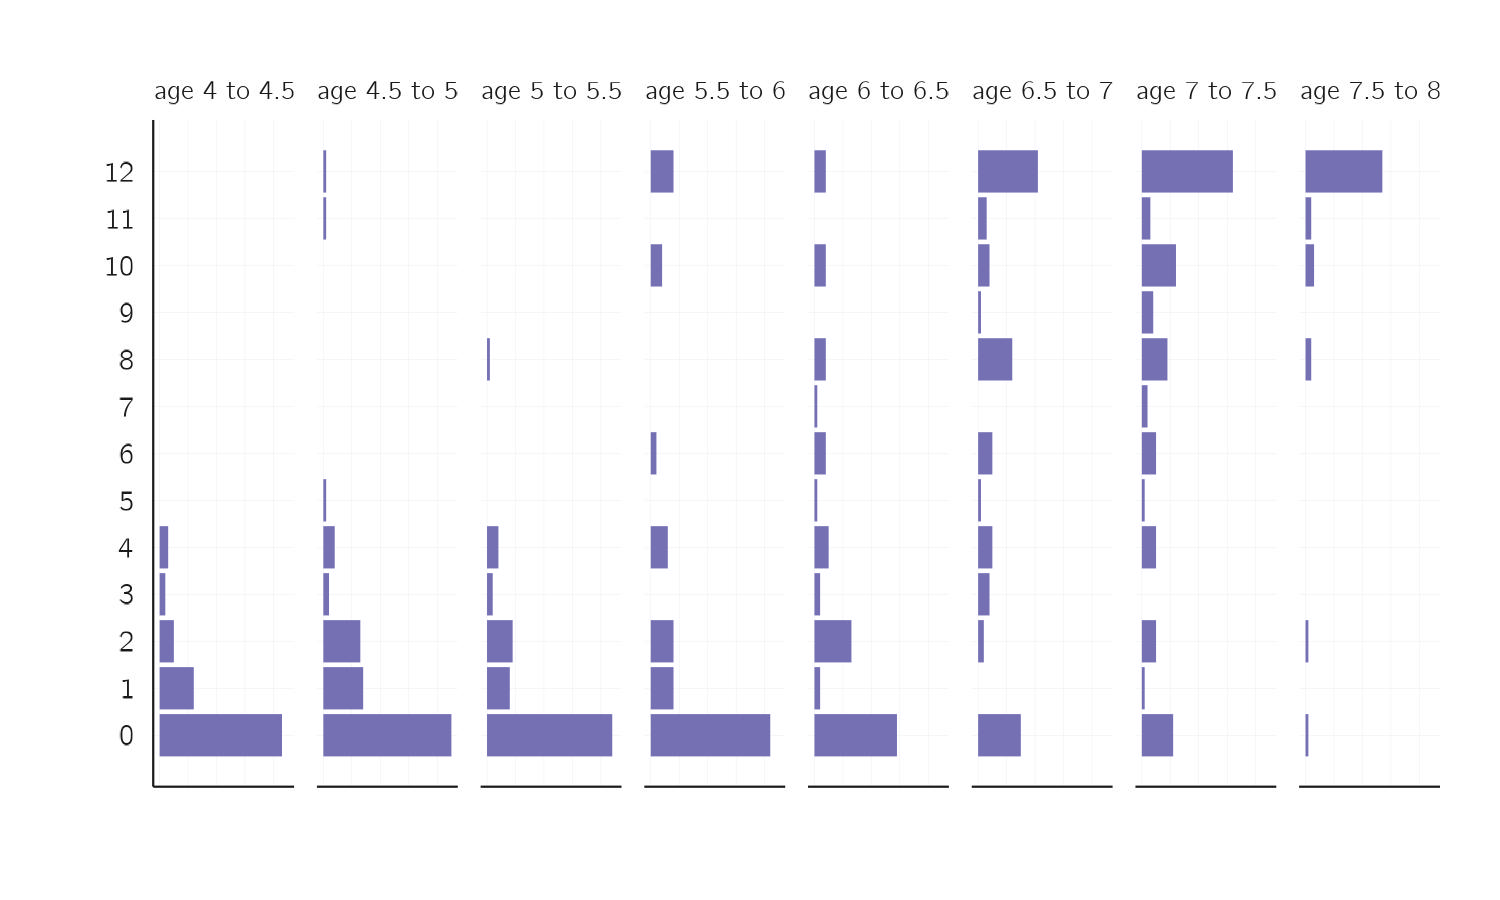
\includegraphics[width=9.375in,height=\textheight]{media/ch3/fig-ch3-img25-old-37.jpg}

}

\caption{\label{fig-ch3-img25-old-37}The Bentler conservation data.}

\end{figure}%

A great exercise we have often used in the classroom is to build a
Zeeman machine, collect data with it, and fit the cusp model to the data
(see Grasman, van der Maas, and Wagenmakers 2009 for details). Zeeman
invented this machine to demonstrate the properties of the cusp. Our
students were rewarded for the quality of the model and the artistic
value of their Zeeman machine (figure~\ref{fig-ch3-img26-old-38}).

\begin{figure}

\centering{

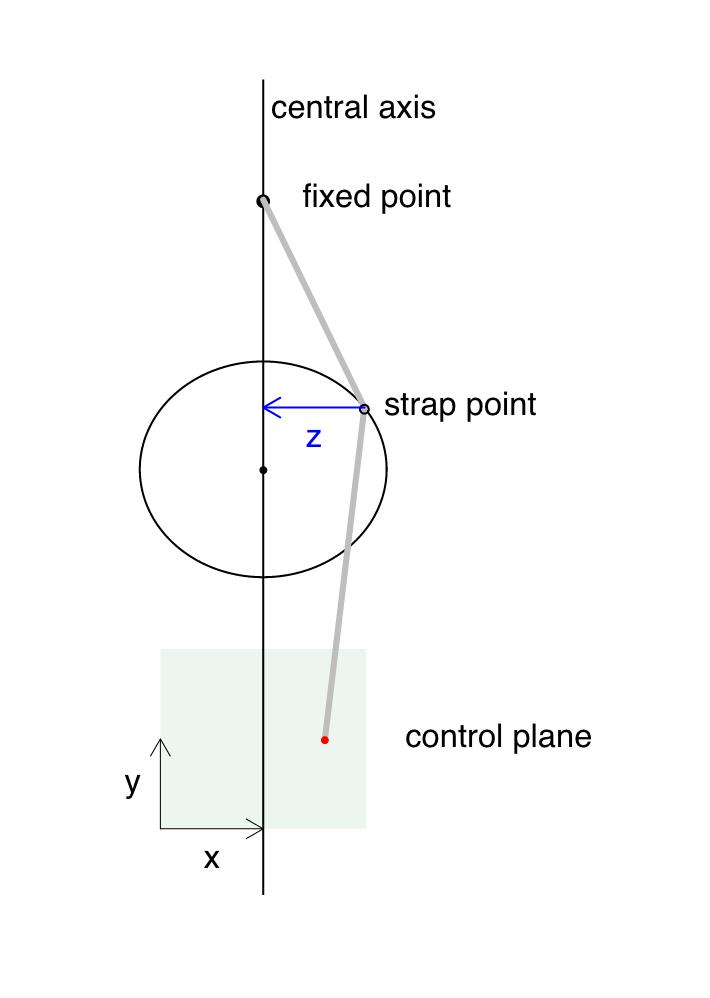
\includegraphics[width=8cm,height=\textheight]{media/ch3/image26.jpg}

}

\caption{\label{fig-ch3-img26-old-38}Zeeman's catastrophe machine. It
consists of a rotating disk and two elastic bands. The first elastic
band is attached to a fixed point and the strap point. The end of the
other elastic (red dot) is moved by hand through the control plan. The
strap point moves according to the cusp catastrophe. Data is gathered by
collecting a set of X, Y, and Z values. Typically, 50 to 100 data points
are sufficient to run cusp fit function in R.}

\end{figure}%

\subsubsection{Evaluation}\label{sec-Evaluation}

A few final remarks: First, Cobb's method can be used with
cross-sectional data. {\marginnote{\begin{footnotesize}Cobb's method is
not valid for time series.\end{footnotesize}}} Data points should be
independent. To test for hysteresis in time series, other approaches are
required. One option is to use hidden Markov models as in Dutilh et al.
(2011).

Second, there are some issues with Cobb's approach that are due to
fundamental differences between probability distributions and potential
functions. The latter can be transformed in many ways (so-called local
diffeomorphisms) without changing the qualitative properties of the
cusp. With the added constraint on probability distributions (area = 1),
the same transformations can lead to qualitative effects, such as a
change in the number of modes. Wagenmakers et al. (2005) suggest a
solution to this problem for time series.

Third, two alternative approaches have been proposed. Both Guastello's
(1982) change score least square regression approach and the Gemcat
approach (1987) use the first derivative of the cusp as point of
departure. A problem with both approaches is that they do not
distinguish between stable and unstable equilibrium states. Data points
in the inaccessible region improve the fit of the model, whereas they
should decrease the fit. Alexander et al. (1992) provide a detailed
critique.

\section{Criticism of catastrophe
theory}\label{sec-Criticism-of-catastrophe-theory}

Rosser (2007) speaks of the rise and the fall of catastrophe theory. The
hype following the publication of Zeeman (1976) in Scientific American
\footnote{To see Zeeman at work, I recommend the BBC documentary
  \emph{Case Study Catastrophe Theory Maths Foundation Course}
  (\url{https://www.youtube.com/watch?v=myDvcvox1V4&t=1435s}).}, in
which he introduced the phenomenological application of catastrophe
theory in the behavioral and social sciences, led to a strongly worded
reply by Zahler and Sussmann (1977) in Nature.

Because people still refer to Zeeman's paper when we use catastrophe
theory in our work, I will briefly respond to Zahler and Sussmann's main
points of criticism. In their introduction, they state that there may be
legitimate uses of catastrophe theory in physics and engineering.
{\marginnote{\begin{footnotesize}They do not question the correctness or
importance of catastrophe theory as a purely mathematical
subject.\end{footnotesize}}}

They raise 10 points, some of which I have already addressed. For
example, their first point is about how sudden a jump actually is, but
they call this a less serious criticism. As I explained earlier, it is
not the suddenness that matters but whether or not the intermediate
states are unstable.

A number of points are about inferring a cusp from data, which was
indeed done rather superficially in Zeeman's earlier work. They point
out that there are no testable predictions, that the location of the
cusp can be shifted, and that there is no way to decide whether the data
fit the cusp. I hope to have shown that these problems are largely
solved: the catastrophe flags allow us to make new testable predictions,
and with Cobb's maximum likelihood approach we can fit the model as we
would do with any other statistical model in modern science. Of course,
one can be critical of the use of statistics in psychology and the
social sciences, but these criticisms are not specific to catastrophe
theory.

Another, somewhat inconsistent, line of criticism is that many
catastrophe models in psychology and the social sciences are just wrong
and inconsistent with the data (which could be true), and they also
claim that Zeeman's models are not falsifiable. But you cannot have it
both ways: if it is wrong or inconsistent with the data, it is
falsifiable. Nevertheless, I agree that it is important to think about
falsifiability. Theories in psychology tend to be moving targets. As
soon as someone finds an empirical result that contradicts the theory,
the theory is quickly modified.

Then Zahler and Sussmann point out that catastrophe theorists often try
to make a discrete variable into a continuous one. Their example is
aggression, which they believe is inherently discrete. They call
Zeeman's interpretation of aggression as a continuous family of
behaviors absurd and utterly meaningless. This may be a bit strong. We
can think of situations in which aggression can vary from mild to
severe, or from verbal to physical, directed at a person's belongings,
mild physical directed at the person, to severe physical. A rich
ordering of aggressive acts is very useful for describing domestic
violence. Sometimes the change along these acts or variants is gradual,
and other times sudden. Whether such an ordering can be treated as a
quantitative continuum is one of the most difficult questions in our
field (Borsboom et al. 2016; Michell 2008).

Zahler and Sussmann's final point is that there are better alternatives,
such as quantum mechanics, discrete mathematics, and bifurcation theory.
There is work on quantum mechanics in psychology (especially in the
context of consciousness), but whether it will lead to breakthroughs in
this field remains to be seen. Discrete mathematics may be an
alternative in some cases (e.g., to model symbolic thinking). I see
catastrophe theory as a special branch of bifurcation theory, especially
useful when the system under study is difficult to describe in terms of
mathematical equations. This goes back to the distinction between
phenomenological and mechanistic models. I think we should put more
effort into developing mechanistic models based on first principles.
More on this in the next chapters.

Loehle (1989) presents an excellent discussion on the usefulness of
catastrophe theory in the context of modeling ecosystems. He concludes
that ``an unresolved problem in applying catastrophe models is that of
testing the goodness of fit of the model to data,'' but this problem has
now been largely solved. {\marginnote{\begin{footnotesize}The empirical
program, using catastrophe flags in conjunction with Cobb's method for
fitting cusp models, bypasses much of the previous criticism of
catastrophe theory.\end{footnotesize}}}

\section{Conclusion}\label{sec-Conclusion-ch3}

Psychologists are often concerned with psychological types and classes,
stages and phases, and the transitions between them. Our thinking about
transitions becomes much clearer and more advanced when we know the
basics of bifurcations.

Catastrophe theory comes with a toolbox for the behavioral and social
sciences. We can build phenomenological models, test for catastrophe
flags, and even fit cusp models to data. With the development of this
toolbox, most of the criticisms of catastrophe theory lose their
relevance.

However, there is room for improvement. Phenomenological models have
limited explanatory power. As explained in the next chapter on dynamical
system models, it is possible to create more mechanistic models that
support the use of phenomenological models. In Chapter 6,
section~\ref{sec-Ising-attitude-model}, another option is introduced
using networks. I will demonstrate that the behavior of the Ising
network model for attitudes is governed by the cusp model, which is very
similar to the cusp model proposed for the attitude toward abortion.

\section{Exercises}\label{sec-Exercises-ch3}

\begin{enumerate}
\def\labelenumi{\arabic{enumi})}
\item
  The equilibria of the fold are \(X = \pm \sqrt{\frac{a}{3}}\). This
  can can be checked by setting the first derivative to 0. Show this.
  (*)
\item
  In Zeeman's dog aggression model, fear and rage are ``rotated''
  control variables. How can we translate this to a model with unrotated
  axes? Provide the equations that specify the normal and splitting axis
  as function of fear and rage. (*)
\item
  Derive the equation for the bifurcation lines of the cusp
  (\(27a^{2} = 4b^{3})\), by setting the first and second derivatives to
  0. Plot the bifurcation lines in GeoGebra or Desmos. (**)
\item
  Some insight into the butterfly catastrophe
  \(V(X) = {- aX - bX^{2} - cX}^{3} - dX^{4} + X^{6}\) can be gained by
  entering the equation in free online graphing calculators such as
  Desmos or GeoGebra. Set \(a\), \(b\), \(c\), \(d\) to 0, -5, 0, 5.
  Then start varying \(a\) and \(c\). What is the difference in the
  effect of these two parameters on the appearance and disappearance of
  attractors? (*)
\item
  Set up a phenomenological cusp for falling in love. Follow my
  guidelines (see section~\ref{sec-Phenomenological-models}). (**)
\item
  Check whether indeed the Bentler data fit better when
  \texttt{age\_range} only loads on the normal axis (according to the
  AIC and BIC). What is the correct specification of \texttt{beta} in
  \texttt{cusp()} in this case? (*)
\item
  What is the best fitting cusp model (according to the BIC) for this
  tricky dataset created with this R code? Why? (**)

\begin{Shaded}
\begin{Highlighting}[]
\NormalTok{n}\OtherTok{=}\DecValTok{500}
\NormalTok{z }\OtherTok{=} \FunctionTok{Vectorize}\NormalTok{(rcusp)(}\DecValTok{1}\NormalTok{, .}\DecValTok{7}\SpecialCharTok{*}\FunctionTok{rnorm}\NormalTok{(n), }\DecValTok{2}\SpecialCharTok{+}\DecValTok{2}\SpecialCharTok{*}\FunctionTok{rnorm}\NormalTok{(n)) }\CommentTok{\# sample z }
\NormalTok{x }\OtherTok{=} \FunctionTok{rnorm}\NormalTok{(n) }
\NormalTok{y }\OtherTok{=} \FunctionTok{rnorm}\NormalTok{(n) }
\NormalTok{data }\OtherTok{\textless{}{-}} \FunctionTok{data.frame}\NormalTok{(z,x,y) }\CommentTok{\# collect variables in data}
\end{Highlighting}
\end{Shaded}
\item
  Build a Zeeman machine, collect data, and fit the cusp (see Example
  III of Grasman, van der Maas, and Wagenmakers 2009). What is your best
  fitting model? Provide a plot of the data in the bifurcation set and a
  picture of your Zeeman machine. (**)
\end{enumerate}

\bookmarksetup{startatroot}

\chapter{Building dynamic system models}\label{sec-ch4n}

Suppose you are in a bar in Amsterdam and someone asks if you would like
another beer. The number of drinks you have already had will probably
influence your decision. Perhaps your self-control, whatever it may be,
kicks in and you refuse, even though the alcohol already in your system
may be interfering with that self-control. Or you may have reached your
limit and simply collapse. In this chapter, we will see how such a
decision-making process can be modeled using nonlinear differential
equations.

This form of modeling is often called nonlinear dynamical systems theory
(NLDST), another branch of the complex-systems approach.
{\marginnote{\begin{footnotesize}A nonlinear dynamical system is one in
which the change of system variables over time is governed by nonlinear
equations, resulting in complex behavior such as chaos and
bifurcations.\end{footnotesize}}} We saw examples of nonlinear dynamical
system models in earlier chapters. The logistic map is an example of a
discrete-time nonlinear dynamical model defined as a difference
equation. The catastrophe models are also dynamical systems governed by
a potential function. In Chapter 3,
section~\ref{sec-Building-catastrophe-models}, I made a distinction
between phenomenological modeling (assuming the cusp) and mechanistic
modeling (deriving the cusp from first principles). Here we will focus
on the more mechanistic construction of dynamical system models.

In psychology, following the principle of parsimony (Occam's razor), we
must start with simple models. We don't have many first principles to
start with, and our data are often limited, making model testing
difficult. But we can learn a lot from other disciplines. Nonlinear
dynamical systems have been developed in all the natural sciences, but
my main inspiration comes from mathematical biology, especially
ecological modeling (Murray 1989). Mathematical psychology is generally
less developed than mathematical biology, but this depends somewhat on
the subfield. In areas such as neural modeling, speeded-decision making,
memory, choice, and psychometrics, there are advanced models, and I will
provide some examples later in this chapter.

I will first present a basic overview of dynamical systems modeling in
other sciences. Then I will discuss applications in psychology. I refer
to more advanced sources when necessary. I recommend the book by Gottman
et al. (2002) for its clear and basic explanation of the mathematical
aspects of dynamical systems modeling. Strogatz's online lectures on
nonlinear dynamics and chaos and his book (2018) are very helpful.
Murray's book (2002) on mathematical biology is also highly recommended.
Meadows's \emph{Thinking in Systems} (2008) offers a basic introduction.

This chapter will be hands-on again. We will use the Grind package in R
to simulate dynamical systems models. Grind (de Boer 2018) is based on
the R packages deSolve and rootSolve (Soetaert, Petzoldt, and Setzer
2010). It facilitates numerical integration, phase plane analysis, and
stability analysis of steady states.\footnote{The manual can be found at
  \url{https://github.com/hansschepers/grindr/blob/master/inst/documentation/GRIND\%20tutorial.pdf.}}

At the end of the chapter, I will introduce causal-loop diagrams and an
open-source tool, Insightmaker, that makes it easy to create causal-loop
diagrams. We will also use Insightmaker to simulate dynamical systems
models, for which I will provide some examples.

\section{Basic concepts}\label{sec-Basic-concepts}

\subsection{Back to the logistic
equation}\label{sec-Back-to-the-logistic-equation}

We saw the logistic equation in the form of the logistic map
(section~\ref{sec-The-population-growth-of-rabbits}), where time
progressed in discrete steps. The logistic map is a difference equation,
\(X_{t + 1} = f(X_{t})\), but in this chapter we will focus on
differential equations in continuous time. We will limit ourselves to
ordinary differential equations (ODEs).
{\marginnote{\begin{footnotesize}In ordinary differential equations, we
take the derivatives with respect to only one
variable.\end{footnotesize}}} The ODE for logistic growth\footnote{In
  many texts \(\frac{dX}{dt}\) is written as \(\dot{X}\).} is:

\begin{equation}\phantomsection\label{eq-ch4n-1-old-21}{
\frac{dX}{dt} = rX(1 - X).
}\end{equation}

The change in \(X\) is a function of \(X\) itself. The exponential
growth term \(rX\) dominates when \(X\) is close to 0, but the growth
levels off as \(X\) approaches 1. A solution to this equation expresses
\(X_{t}\) as a function of the initial state \(X_{0}\). In simple cases
we can do this using the math we learned in high school. For exponential
growth \(dX/dt = rX\), this is the derivation:

\begin{longtable}[]{@{}
  >{\raggedright\arraybackslash}p{(\columnwidth - 2\tabcolsep) * \real{0.6067}}
  >{\raggedright\arraybackslash}p{(\columnwidth - 2\tabcolsep) * \real{0.3933}}@{}}
\toprule\noalign{}
\endhead
\bottomrule\noalign{}
\endlastfoot
\(\frac{dX}{dt} = rX\)

\(\frac{dX}{X} = rdt\) & by separation of variables \\
\(\int_{}^{}\frac{dX}{X} = \int_{}^{}{rdt}\) & integrate \\
\(\ln X = rt + C\) & assuming \(X \geq 0\) \\
\(X = e^{rt + C} = e^{C}e^{rt}\) & by taking the exponent \\
\(X_{0} = e^{C}e^{r0} \Longrightarrow X_{0} = e^{C}\) & compute the
integration constant \\
\end{longtable}

\begin{equation}\phantomsection\label{eq-ch4n-2-old-22}{
\Longrightarrow X_{t} = {X_{0}e}^{rt}
}\end{equation}

But for more complex models, such an analytical solution is out of scope
and numerical solutions (by simulation) are required. This is not the
preferred choice. These simulations can be slow, they may accumulate
rounding errors, and it can be difficult to search the entire parameter
space, especially when multiple parameters are involved.

The naive implementation of differential equations in R is risky. This
would involve a for loop:

\begin{Shaded}
\begin{Highlighting}[]
\NormalTok{x }\OtherTok{\textless{}{-}}\NormalTok{ x0 }\OtherTok{\textless{}{-}}\NormalTok{ .}\DecValTok{1}  \CommentTok{\# initial value}
\NormalTok{r }\OtherTok{\textless{}{-}}\NormalTok{ .}\DecValTok{5} \CommentTok{\# growth rate}
\NormalTok{dt }\OtherTok{\textless{}{-}}\NormalTok{ .}\DecValTok{00001} \CommentTok{\# time step in simulation}
\NormalTok{t }\OtherTok{\textless{}{-}} \DecValTok{10}  \CommentTok{\# Nt, time we want to know the value of x}
\NormalTok{timesteps }\OtherTok{\textless{}{-}}\NormalTok{ t}\SpecialCharTok{/}\NormalTok{dt }\CommentTok{\# required time steps given t and dt}
\ControlFlowTok{for}\NormalTok{(i }\ControlFlowTok{in} \DecValTok{2}\SpecialCharTok{:}\NormalTok{timesteps) }\CommentTok{\# note the 2 to use the starting value}
\NormalTok{\{}
\NormalTok{  x[i] }\OtherTok{\textless{}{-}}\NormalTok{ x[i}\DecValTok{{-}1}\NormalTok{] }\SpecialCharTok{+}\NormalTok{ r}\SpecialCharTok{*}\NormalTok{x[i}\DecValTok{{-}1}\NormalTok{]}\SpecialCharTok{*}\NormalTok{dt}
\NormalTok{\}}
\NormalTok{x0}\SpecialCharTok{*}\FunctionTok{exp}\NormalTok{(r}\SpecialCharTok{*}\NormalTok{timesteps}\SpecialCharTok{*}\NormalTok{dt) }\CommentTok{\# analytical solution}
\NormalTok{x[timesteps] }\CommentTok{\# compare}
\NormalTok{timesteps }\CommentTok{\# length of simulation}
\end{Highlighting}
\end{Shaded}

where \(dt\) must be chosen by hand. If you test some values of \(dt\),
you will see that a value too high (.5) leads to a solution
(\texttt{x{[}timesteps{]}}) that is different from the analytical
solution. But if we set \(dt\) very low (.00001), it takes unnecessarily
long.

This is why we use solvers, numerical methods for ordinary differential
equations. {\marginnote{\begin{footnotesize}Solvers are specialized
algorithms designed to numerically approximate solutions to ODEs and
handle the complexities of integrating these equations over time to
predict the evolution of system states under different initial
conditions and parameters.\end{footnotesize}}} We will use the R package
Grind, although many other methods are available in R. One could also
directly use the R packages deSolve and rootSolve by Soetaert, Petzoldt,
and Setzer (2010), on which the Grind package is based. Grind has to be
installed from GitHub using:

\begin{Shaded}
\begin{Highlighting}[]
\FunctionTok{install.packages}\NormalTok{(}\StringTok{"remotes"}\NormalTok{)}
\NormalTok{remotes}\SpecialCharTok{::}\FunctionTok{install\_github}\NormalTok{(}\StringTok{"hansschepers/grindr"}\NormalTok{)}
\end{Highlighting}
\end{Shaded}

The packages required are:

\begin{Shaded}
\begin{Highlighting}[]
\FunctionTok{library}\NormalTok{(deSolve)}
\FunctionTok{library}\NormalTok{(rootSolve)}
\FunctionTok{library}\NormalTok{(FME)}
\FunctionTok{library}\NormalTok{(Grind)}
\end{Highlighting}
\end{Shaded}

The code consists of defining the model, the parameters \(p\), and the
initial values \(s\). Main functions are \texttt{run()},
\texttt{plane()}, \texttt{newton()}, \texttt{continue()}, and
\texttt{fit()}. They will be introduced using examples. With
\texttt{run()} we generate a time series for the model.

\begin{Shaded}
\begin{Highlighting}[]
\NormalTok{model }\OtherTok{\textless{}{-}} \ControlFlowTok{function}\NormalTok{(t, state, parms) \{}
  \FunctionTok{with}\NormalTok{(}\FunctionTok{as.list}\NormalTok{(}\FunctionTok{c}\NormalTok{(state,parms)), \{}
\NormalTok{    dX }\OtherTok{\textless{}{-}}\NormalTok{ r}\SpecialCharTok{*}\NormalTok{X            }\CommentTok{\# the exponential model}
      \FunctionTok{return}\NormalTok{(}\FunctionTok{list}\NormalTok{(}\FunctionTok{c}\NormalTok{(dX)))}
\NormalTok{  \})}
\NormalTok{\}}
\NormalTok{p }\OtherTok{\textless{}{-}} \FunctionTok{c}\NormalTok{(}\AttributeTok{r=}\NormalTok{.}\DecValTok{5}\NormalTok{) }\CommentTok{\# parameter r}
\NormalTok{s }\OtherTok{\textless{}{-}} \FunctionTok{c}\NormalTok{(}\AttributeTok{X=}\NormalTok{.}\DecValTok{1}\NormalTok{) }\CommentTok{\# initial value}
\FunctionTok{run}\NormalTok{(}\AttributeTok{tmax=}\DecValTok{5}\NormalTok{) }\CommentTok{\# run until t = 5, numerical solution}
\NormalTok{s[}\StringTok{\textquotesingle{}X\textquotesingle{}}\NormalTok{]}\SpecialCharTok{*}\FunctionTok{exp}\NormalTok{(p[}\StringTok{\textquotesingle{}r\textquotesingle{}}\NormalTok{]}\SpecialCharTok{*}\DecValTok{5}\NormalTok{) }\CommentTok{\# compare with analytical solution}
\end{Highlighting}
\end{Shaded}

We don't have to worry about time steps anymore, and the numerical and
analytical solutions converge. This is of course a trivial use of an ODE
solver, but much more can be done.

In analyzing the behavior of a dynamical system, first we want to know
what the equilibria \(X^{*}\) are\emph{.} To do this, we need to set the
time derivative equal to 0, \(dX/dt = 0\). For the exponential function,
this is simply \(rX = 0\), that is, when \(X\) is 0 Second, we want to
determine whether these equilibria are stable or unstable. Whether
\(X^{*}=0\) is stable can be determined by checking the second
derivative in \(X^{*}\). If this derivative is less than 0, then the
fixed point is stable. The second derivative is \(r\), so \(X^{*} = 0\)
is an unstable fixed point whenever \(r > 0\) and stable whenever
\(r < 0\). You can check this in Grind by using\(\ r\) values of -.1 and
.1, and start values equal to or just above or below 0.

For equation~\ref{eq-ch4n-1-old-21}, the logistic function, we also want
to know the equilibria, the stable and unstable fixed points. To do so
we follow the same steps as for the exponential function (see
exercises).

The continuous-time implementation of the logistic function is somewhat
boring compared to its discrete-time variant that we studied in
section~\ref{sec-The-population-growth-of-rabbits}. The difference is
that the overshooting and undershooting do not occur in continuous time.
By changing the logistic model in Grind to:\footnote{The \(-X\) is added
  because the difference equation has the form \(X_{t + 1} = f(X_{t})\),
  so the change \(dX\) is thus \(f(X_{t})-X_{t}\).}

\begin{Shaded}
\begin{Highlighting}[]
\NormalTok{dX }\OtherTok{\textless{}{-}}\NormalTok{ r}\SpecialCharTok{*}\NormalTok{X}\SpecialCharTok{*}\NormalTok{(}\DecValTok{1}\SpecialCharTok{{-}}\NormalTok{X) }\SpecialCharTok{{-}}\NormalTok{ X }
\end{Highlighting}
\end{Shaded}

and using \texttt{method=\textquotesingle{}euler\textquotesingle{}} in
the \texttt{run()} function, you can simulate the discrete-time logistic
map. Check if you get chaos for \(r = 4\). Use the Euler method only in
special cases, as it is generally the least accurate approach.

\subsection{The Lotka---Volterra
models}\label{sec-The-LotkaVolterra-models}

Perhaps the best-known population models are the Lotka---Volterra
equations (Murray 2002). {\marginnote{\begin{footnotesize}The
Lotka\end{footnotesize}}}---{\marginnote{\begin{footnotesize}Volterra
models describe the dynamics of biological systems in which two species
interact, one as a predator and the other as prey.\end{footnotesize}}}
These consist of coupled differential equations, one for the density of
the prey and one for the density of the predator:

\begin{equation}\phantomsection\label{eq-ch4n-3-old-23}{
\frac{dN}{dt} = aN - bPN
}\end{equation}

\begin{equation}\phantomsection\label{eq-ch4n-4-old-24}{
\frac{dP}{dt} = cPN - dP
}\end{equation}

Where \(N\) and \(P\) refer to the sizes of the prey and predator
populations, \(a\) and \(c\) determine the growth rates, and \(b\) and
\(d\) control the mortality rates. Note that the mortality rate of prey
depends on both \(N\) and \(P\), while the mortality rate of predators
depends only on \(P\). Similarly, the growth terms are also asymmetric,
predators increase as a function of both \(N\) and \(P\), and:they eat
prey. We will follow the simple example provided by Wikipedia (on
Lotka---Volterra equations).

To implement this model in Grind, we use:

\begin{Shaded}
\begin{Highlighting}[]
\NormalTok{LV }\OtherTok{\textless{}{-}} \ControlFlowTok{function}\NormalTok{(t, state, parms) \{}
  \FunctionTok{with}\NormalTok{(}\FunctionTok{as.list}\NormalTok{(}\FunctionTok{c}\NormalTok{(state,parms)), \{}
\NormalTok{    dN }\OtherTok{\textless{}{-}}\NormalTok{ a}\SpecialCharTok{*}\NormalTok{N }\SpecialCharTok{{-}}\NormalTok{ b}\SpecialCharTok{*}\NormalTok{P}\SpecialCharTok{*}\NormalTok{N}
\NormalTok{    dP }\OtherTok{\textless{}{-}}\NormalTok{ c}\SpecialCharTok{*}\NormalTok{P}\SpecialCharTok{*}\NormalTok{N }\SpecialCharTok{{-}}\NormalTok{ d}\SpecialCharTok{*}\NormalTok{P}
    \FunctionTok{return}\NormalTok{(}\FunctionTok{list}\NormalTok{(}\FunctionTok{c}\NormalTok{(dN, dP)))}
\NormalTok{  \})}
\NormalTok{\}}
\NormalTok{p }\OtherTok{\textless{}{-}} \FunctionTok{c}\NormalTok{(}\AttributeTok{a=}\FloatTok{1.1}\NormalTok{,}\AttributeTok{b=}\NormalTok{.}\DecValTok{4}\NormalTok{,}\AttributeTok{c=}\NormalTok{.}\DecValTok{1}\NormalTok{,}\AttributeTok{d=}\FloatTok{0.4}\NormalTok{) }\CommentTok{\# parameters}
\NormalTok{s }\OtherTok{\textless{}{-}} \FunctionTok{c}\NormalTok{(}\AttributeTok{N=}\DecValTok{10}\NormalTok{,}\AttributeTok{P=}\DecValTok{10}\NormalTok{)             }\CommentTok{\# 10 baboons and 10 cheetahs}
\end{Highlighting}
\end{Shaded}

Some typical uses of Grind are:

\begin{Shaded}
\begin{Highlighting}[]
\FunctionTok{layout}\NormalTok{(}\DecValTok{1}\SpecialCharTok{:}\DecValTok{2}\NormalTok{)}
\NormalTok{data}\OtherTok{=}\FunctionTok{run}\NormalTok{(}\AttributeTok{odes=}\NormalTok{LV,}\AttributeTok{tstep=}\NormalTok{.}\DecValTok{01}\NormalTok{,}\AttributeTok{table=}\NormalTok{T) }\CommentTok{\# set tstep to low value}
\CommentTok{\# phase plot for different starting values}
\FunctionTok{plane}\NormalTok{(}\AttributeTok{odes=}\NormalTok{LV,}\AttributeTok{portrait =} \ConstantTok{TRUE}\NormalTok{, }\AttributeTok{ymax=}\DecValTok{17}\NormalTok{, }\AttributeTok{xmax=}\DecValTok{50}\NormalTok{, }\AttributeTok{tstep=}\FloatTok{0.1}\NormalTok{,}\AttributeTok{grid=}\DecValTok{4}\NormalTok{)}
\end{Highlighting}
\end{Shaded}

The plane function makes a phase plot with \(N\) and \(P\) as axes. The
black points are initial states. What we learn from this is that the
equilibrium of the Lotka---Volterra equations is a limit cycle that
depends on the choice of the initial conditions.

A well-known improvement to this model is to make the prey growth
density dependent by using the logistic equation. This can be done by
setting \texttt{dN\ \textless{}-\ a*N\ *(1-N)\ -\ b*P*N} in the model.
This is the case used as an example in the Grind tutorial, which I
highly recommend reading (de Boer 2018). It also contains the
appropriate parameter values for this model variant. In this
density-dependent model, there are fixed points, in contrast to the
original model. This shows that such model choices can have a large
effect.

A famous example of a system of three coupled differential equations is
the Susceptible-Infected-Recovered (SIR) model used to model infectious
diseases and to understand the impact of interventions on disease
dynamics. {\marginnote{\begin{footnotesize}The
Susceptible-Infected-Recovered (SIR) model is a basic epidemiological
model that divides a population into susceptible (S), infected (I), and
recovered (R) individuals.\end{footnotesize}}} The states of the model
are susceptible, representing individuals who have not yet contracted
the disease but are at risk; infected, representing individuals who are
currently infected and can transmit the disease to susceptible
individuals; and recovered, representing individuals who have recovered
from the disease and are assumed to be immune and no longer susceptible.
The differential equations specify the change in susceptible, infected,
and recovered members of the population. You can now easily implement
this model yourself (see exercises).

\subsection{Fitting models: Stochasticity versus
noise}\label{sec-Fitting-models-stochasticity-versus-noise}

Grind includes an option to fit dynamical systems models. With
\texttt{fit()}, based on the \texttt{modFit()} function from the FME
package (Soetaert, Petzoldt, and Setzer 2010), one can estimate the
model parameters given a dataset. These functions also provide
confidence intervals and allow fixing parameters and bootstrap analysis.
Fitting nonlinear dynamical systems models to data is an art in itself.
For example, these methods can be very sensitive to the choice of
initial values.

I will illustrate the use of \texttt{fit()} on three datasets created
with the original Lotka---Volterra model from the previous section. The
first dataset is the deterministic dataset, the data that follow
directly from the code above. The second is created using a stochastic
Lotka---Volterra model. I will explain how this works in the next
section. The third is a deterministic dataset with measurement error. We
will see that the last two cases are very different.

\begin{Shaded}
\begin{Highlighting}[]
\FunctionTok{set.seed}\NormalTok{(}\DecValTok{1}\NormalTok{)}
\FunctionTok{layout}\NormalTok{(}\FunctionTok{matrix}\NormalTok{(}\DecValTok{1}\SpecialCharTok{:}\DecValTok{4}\NormalTok{,}\DecValTok{2}\NormalTok{,}\DecValTok{2}\NormalTok{,}\AttributeTok{byrow=}\NormalTok{T))}
\NormalTok{p }\OtherTok{\textless{}{-}} \FunctionTok{c}\NormalTok{(}\AttributeTok{a=}\FloatTok{1.1}\NormalTok{,}\AttributeTok{b=}\NormalTok{.}\DecValTok{4}\NormalTok{,}\AttributeTok{c=}\NormalTok{.}\DecValTok{1}\NormalTok{,}\AttributeTok{d=}\FloatTok{0.4}\NormalTok{) }\CommentTok{\# p is a named vector of parameters}
\NormalTok{s }\OtherTok{\textless{}{-}} \FunctionTok{c}\NormalTok{(}\AttributeTok{N=}\DecValTok{10}\NormalTok{,}\AttributeTok{P=}\DecValTok{10}\NormalTok{)             }\CommentTok{\# s is the state}
\NormalTok{n }\OtherTok{\textless{}{-}} \DecValTok{30}
\NormalTok{data\_deterministic }\OtherTok{\textless{}{-}} \FunctionTok{run}\NormalTok{(}\AttributeTok{odes=}\NormalTok{LV,n,}\AttributeTok{table=}\NormalTok{T,}\AttributeTok{timeplot =}\NormalTok{F) }\CommentTok{\# deterministic data}
\NormalTok{data\_stochastic }\OtherTok{\textless{}{-}} \FunctionTok{run}\NormalTok{(}\AttributeTok{odes=}\NormalTok{LV,n,}\AttributeTok{table=}\NormalTok{T,}\AttributeTok{after=}\StringTok{"state\textless{}{-}state+rnorm(2,0,.1)"}\NormalTok{,}
                       \AttributeTok{timeplot =}\NormalTok{F) }\CommentTok{\# add stochasticity}
\NormalTok{data\_error }\OtherTok{\textless{}{-}} \FunctionTok{run}\NormalTok{(}\AttributeTok{odes=}\NormalTok{LV,n,}\AttributeTok{table=}\NormalTok{T,}\AttributeTok{timeplot =}\NormalTok{F)}
\NormalTok{data\_error[,}\DecValTok{2}\SpecialCharTok{:}\DecValTok{3}\NormalTok{] }\OtherTok{\textless{}{-}}\NormalTok{ data\_error[,}\DecValTok{2}\SpecialCharTok{:}\DecValTok{3}\NormalTok{]}\SpecialCharTok{+}
  \FunctionTok{matrix}\NormalTok{(}\FunctionTok{rnorm}\NormalTok{(}\DecValTok{2}\SpecialCharTok{*}\NormalTok{n,}\DecValTok{0}\NormalTok{,}\DecValTok{2}\NormalTok{),,}\DecValTok{2}\NormalTok{) }\CommentTok{\# measurement error }
\CommentTok{\#fit \& plot}
\NormalTok{s}\OtherTok{\textless{}{-}}\NormalTok{ s}\SpecialCharTok{*}\FunctionTok{abs}\NormalTok{(}\FunctionTok{rnorm}\NormalTok{(}\DecValTok{2}\NormalTok{,}\DecValTok{1}\NormalTok{,}\FloatTok{0.1}\NormalTok{));s; p}\OtherTok{\textless{}{-}}\NormalTok{ p}\SpecialCharTok{*}\FunctionTok{abs}\NormalTok{(}\FunctionTok{rnorm}\NormalTok{(}\DecValTok{4}\NormalTok{,}\DecValTok{1}\NormalTok{,}\FloatTok{0.1}\NormalTok{));p    }\CommentTok{\# start values}
\NormalTok{f\_deter}\OtherTok{\textless{}{-}} \FunctionTok{fit}\NormalTok{(}\AttributeTok{odes=}\NormalTok{LV,data\_deterministic,}\AttributeTok{main=}\StringTok{\textquotesingle{}deterministic\textquotesingle{}}\NormalTok{)}
\NormalTok{f\_stoch}\OtherTok{\textless{}{-}} \FunctionTok{fit}\NormalTok{(}\AttributeTok{odes=}\NormalTok{LV,data\_stochastic,}\AttributeTok{main=}\StringTok{\textquotesingle{}stochastic\textquotesingle{}}\NormalTok{)}
\NormalTok{f\_error}\OtherTok{\textless{}{-}} \FunctionTok{fit}\NormalTok{(}\AttributeTok{odes=}\NormalTok{LV,data\_error,}\AttributeTok{main=}\StringTok{\textquotesingle{}error\textquotesingle{}}\NormalTok{)}
\NormalTok{pars }\OtherTok{\textless{}{-}} \FunctionTok{matrix}\NormalTok{(}\FunctionTok{c}\NormalTok{(f\_deter}\SpecialCharTok{$}\NormalTok{par[}\DecValTok{3}\SpecialCharTok{:}\DecValTok{6}\NormalTok{],f\_stoch}\SpecialCharTok{$}\NormalTok{par[}\DecValTok{3}\SpecialCharTok{:}\DecValTok{6}\NormalTok{],f\_error}\SpecialCharTok{$}\NormalTok{par[}\DecValTok{3}\SpecialCharTok{:}\DecValTok{6}\NormalTok{]),,}\DecValTok{3}\NormalTok{)}
\NormalTok{pars }\OtherTok{\textless{}{-}} \FunctionTok{rbind}\NormalTok{(pars,}\FunctionTok{c}\NormalTok{(}\FunctionTok{summary}\NormalTok{(f\_deter)}\SpecialCharTok{$}\NormalTok{sigma,}
                     \FunctionTok{summary}\NormalTok{(f\_stoch)}\SpecialCharTok{$}\NormalTok{sigma,}\FunctionTok{summary}\NormalTok{(f\_error)}\SpecialCharTok{$}\NormalTok{sigma))}
\FunctionTok{barplot}\NormalTok{(}\FunctionTok{t}\NormalTok{(pars),}\AttributeTok{beside=}\NormalTok{T,}\AttributeTok{names=}\FunctionTok{c}\NormalTok{(}\StringTok{\textquotesingle{}a\textquotesingle{}}\NormalTok{,}\StringTok{\textquotesingle{}b\textquotesingle{}}\NormalTok{,}\StringTok{\textquotesingle{}c\textquotesingle{}}\NormalTok{,}\StringTok{\textquotesingle{}d\textquotesingle{}}\NormalTok{,}\StringTok{\textquotesingle{}Residuals\textquotesingle{}}\NormalTok{),}
        \AttributeTok{legend.text=}\FunctionTok{c}\NormalTok{(}\StringTok{\textquotesingle{}deterministic\textquotesingle{}}\NormalTok{,}\StringTok{\textquotesingle{}stochastic\textquotesingle{}}\NormalTok{,}\StringTok{\textquotesingle{}error\textquotesingle{}}\NormalTok{),}
        \AttributeTok{args.legend=}\FunctionTok{c}\NormalTok{(}\AttributeTok{x=}\DecValTok{13}\NormalTok{))}
\end{Highlighting}
\end{Shaded}

This results in figure~\ref{fig-ch4n-img1-old-49}.

\begin{figure}

\centering{

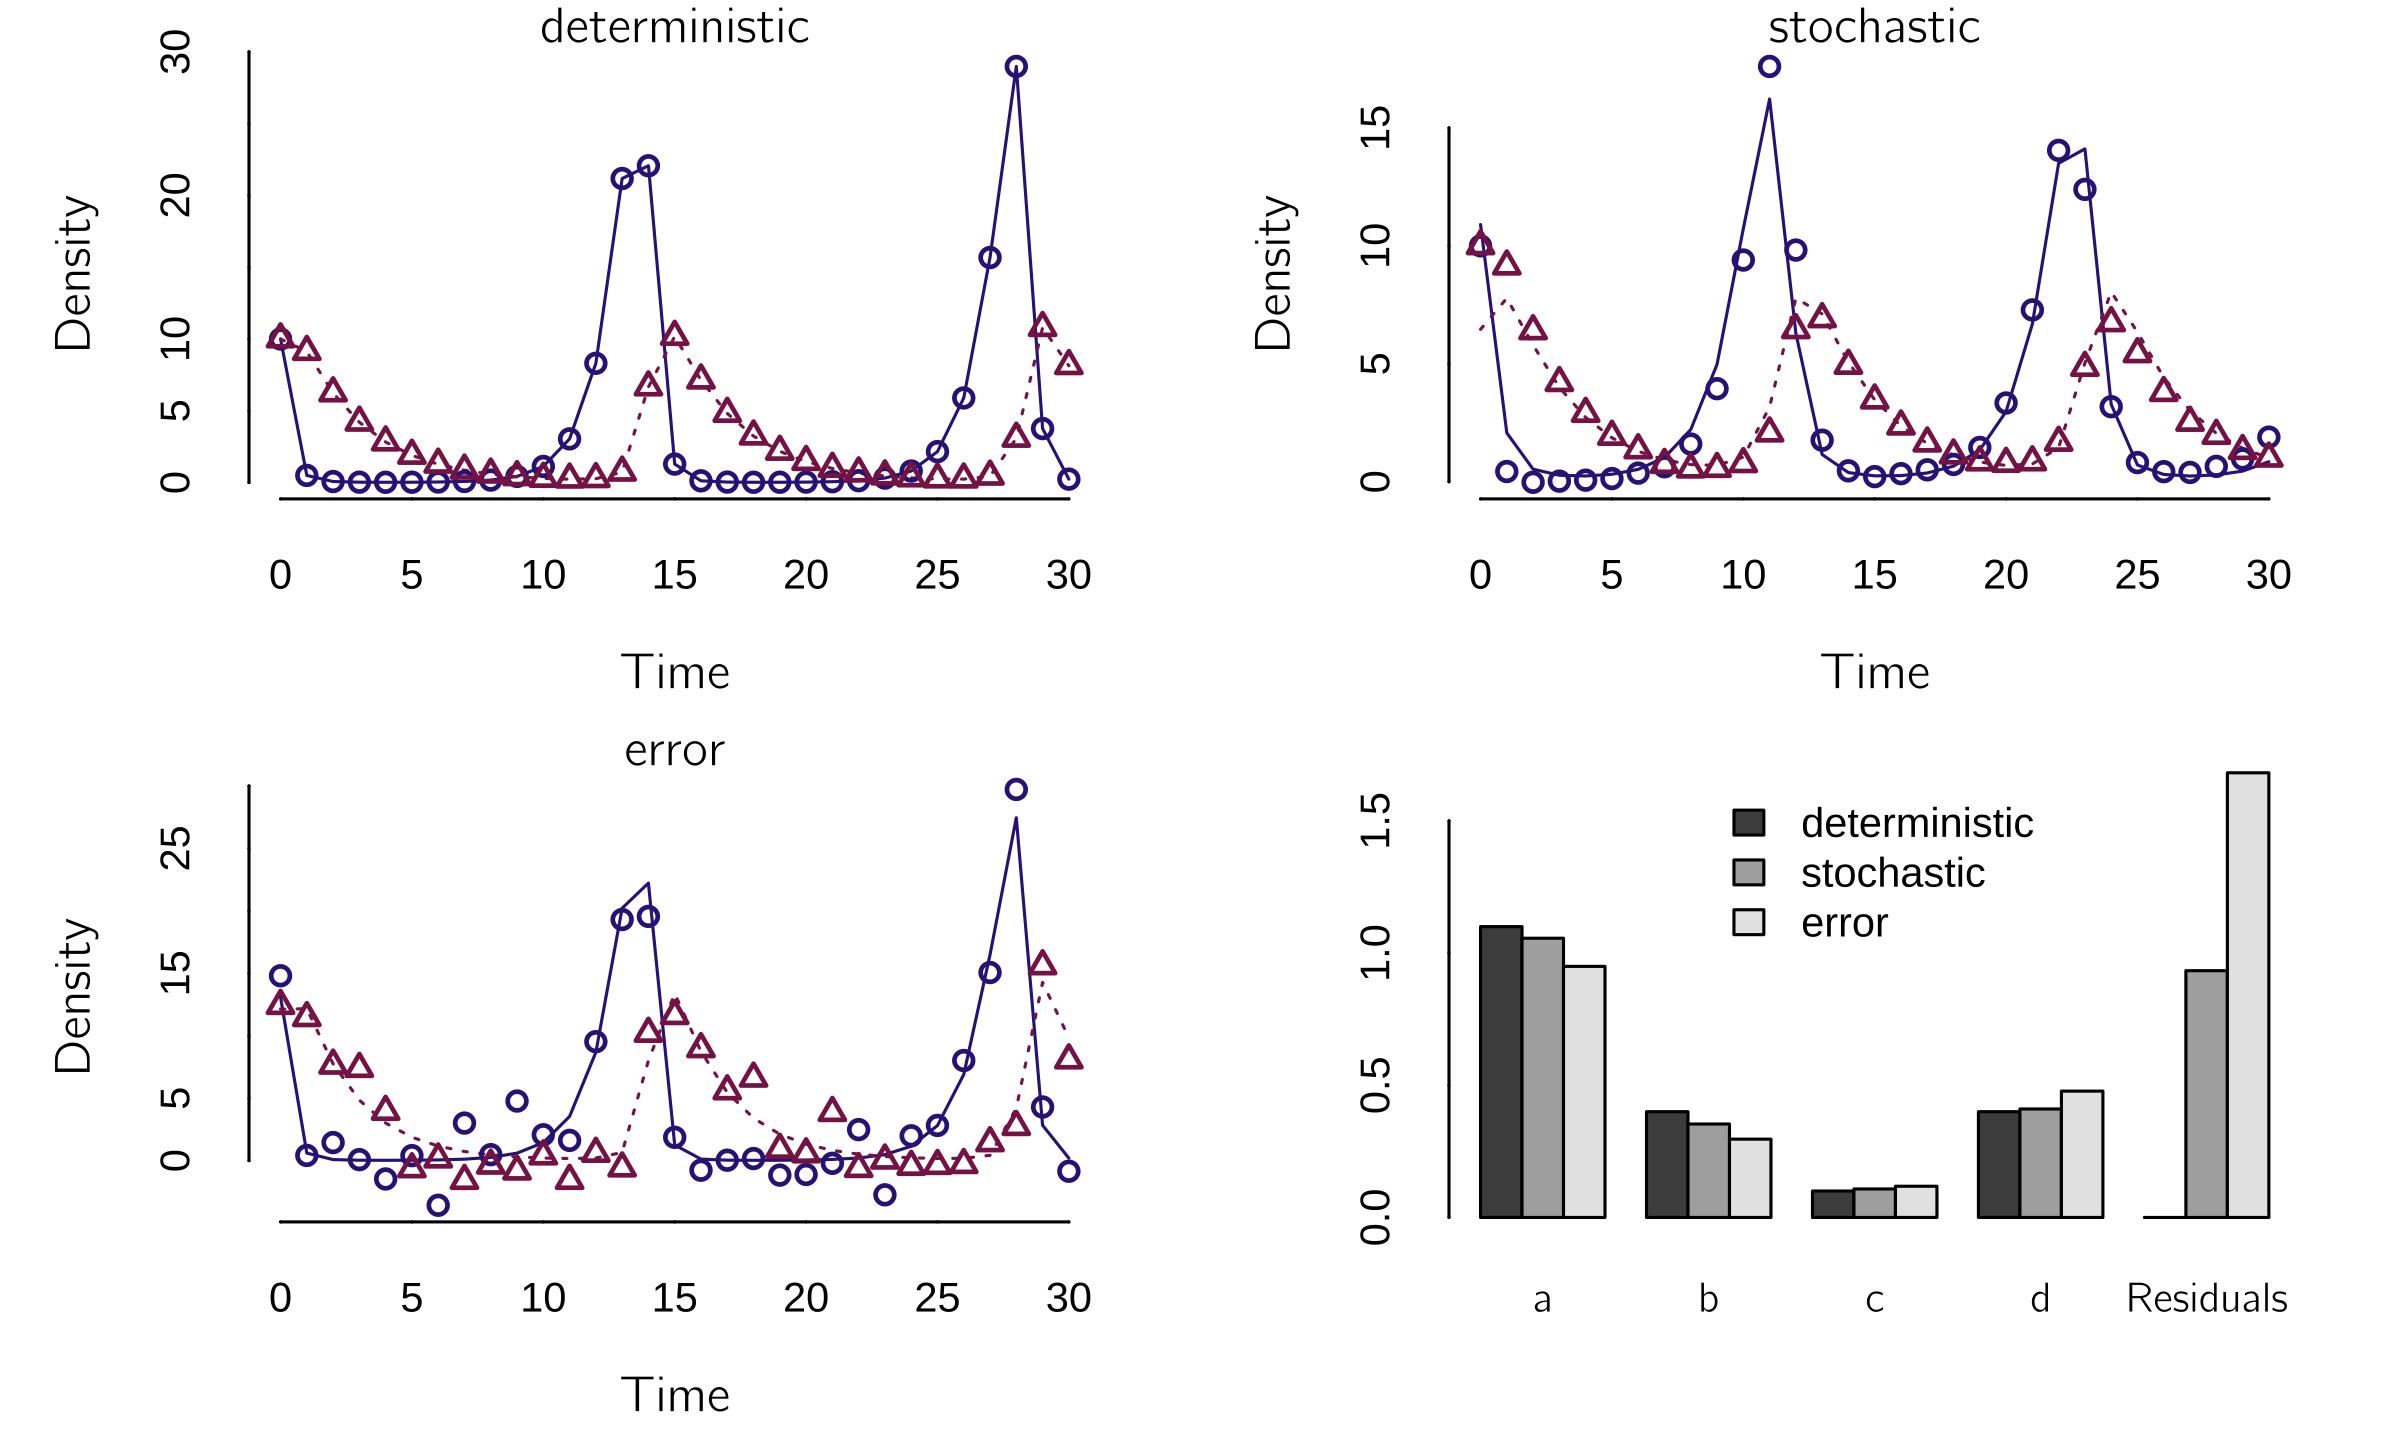
\includegraphics{media/ch4n/fig-ch4n-img1-old-49.png}

}

\caption{\label{fig-ch4n-img1-old-49}Fit of the Lotka---Volterra model
on three types of data. The lines represent the fitted curves. In the
stochastic case, noise is part of the system that affects the
computation of the state at the next time step. In the error case, noise
is a measurement error that does not affect the dynamics.}

\end{figure}%

Note that the error dataset looks very similar to the deterministic
dataset because it contains only the measurement error (\(X\) is true
score + error). The error does not affect the dynamics itself. In the
stochastic case, the error (noise) is added to the states after each
time step, which affects the dynamics. In
figure~\ref{fig-ch4n-img1-old-49}, you can see that the positions of the
waves change. In this well-chosen case, the fit is quite good in all
three cases, and the parameter estimates are all quite close to the true
values. Unfortunately, these results are quite unstable. You can do some
testing yourself.

\subsection{Back to the cusp}\label{sec-Back-to-the-cusp}

To illustrate how Grind can be used to perform bifurcation analysis, we
go back to the cusp. Recall that the differential equation for the cusp
is:

\begin{equation}\phantomsection\label{eq-ch4n-5-old-25}{
\frac{dX}{dt} = - V^{'}(X) = {a + bX - X}^{3}.
}\end{equation}

\begin{Shaded}
\begin{Highlighting}[]
\NormalTok{model }\OtherTok{\textless{}{-}} \ControlFlowTok{function}\NormalTok{(t, state, parms)\{}
  \FunctionTok{with}\NormalTok{(}\FunctionTok{as.list}\NormalTok{(}\FunctionTok{c}\NormalTok{(state,parms)),\{}
\NormalTok{    dX }\OtherTok{\textless{}{-}}\NormalTok{  a }\SpecialCharTok{+}\NormalTok{ b}\SpecialCharTok{*}\NormalTok{X }\SpecialCharTok{{-}}\NormalTok{ X}\SpecialCharTok{\^{}}\DecValTok{3}        \CommentTok{\# cusp}
    \FunctionTok{return}\NormalTok{(}\FunctionTok{list}\NormalTok{(dX))}
\NormalTok{  \})}
\NormalTok{\}}
\NormalTok{p }\OtherTok{\textless{}{-}} \FunctionTok{c}\NormalTok{(}\AttributeTok{a=}\DecValTok{0}\NormalTok{,}\AttributeTok{b=}\DecValTok{1}\NormalTok{); s }\OtherTok{\textless{}{-}} \FunctionTok{c}\NormalTok{(}\AttributeTok{X=}\NormalTok{.}\DecValTok{1}\NormalTok{); }\FunctionTok{run}\NormalTok{(}\AttributeTok{ymin=}\SpecialCharTok{{-}}\DecValTok{1}\NormalTok{)}
\NormalTok{s[}\DecValTok{1}\NormalTok{] }\OtherTok{\textless{}{-}} \SpecialCharTok{{-}}\NormalTok{.}\DecValTok{1}\NormalTok{; }\FunctionTok{run}\NormalTok{(}\AttributeTok{add=}\NormalTok{T)}
\end{Highlighting}
\end{Shaded}

This code simulates two runs demonstrating bistability for \(a = 0\) and
\(b = 1\).

A nicer way to demonstrate bistability in the time series is to make the
system stochastic. This was done in Chapter 3,
section~\ref{sec-Cobbs-maximum-likelihood-approach}, by using a
stochastic differential equation: \(dX = - V^{'}(X)dt + \sigma dW(t)\).
Grind has a great trick for this. With the ``after'' parameter in the
function call, we can add discrete events to the system. ``After'' can
also be used to change parameter or state values after a certain amount
of time or after some condition (see the manual). We use it here to add
a random number sampled from a normal distribution, with a mean of 0 and
a standard deviation of .4, to \(X\). The best way to simulate this in
Grind is using the Euler method with a small time step. The noise term
should be corrected with \(\sqrt{dt}\), as shown in the code. The
Wikipedia page on stochastic differential equations will tell you more
about the underlying ideas.

As can be seen in figure~\ref{fig-ch4n-img2-old-50}, the stochastic
force causes spontaneous jumps between the two modes of the cusp. When
noise or random fluctuations cause the entire equilibrium landscape of a
dynamical system to become observable, it is often referred to as
stochastic resonance. {\marginnote{\begin{footnotesize}Stochastic
resonance is a notable example of how noise, which is often considered
undesirable or disruptive, can actually play a constructive role in
certain systems, helping to reveal hidden patterns and structures that
might otherwise remain obscured.\end{footnotesize}}} You can see this by
comparing the figure with one generated with a standard deviation of .1
or less.

\begin{Shaded}
\begin{Highlighting}[]
\FunctionTok{layout}\NormalTok{(}\FunctionTok{t}\NormalTok{(}\FunctionTok{c}\NormalTok{(}\DecValTok{1}\NormalTok{,}\DecValTok{1}\NormalTok{,}\DecValTok{1}\NormalTok{,}\DecValTok{2}\NormalTok{)))}
\NormalTok{data }\OtherTok{\textless{}{-}} \FunctionTok{run}\NormalTok{(}\AttributeTok{table=}\NormalTok{T,}\AttributeTok{tmax=}\DecValTok{1000}\NormalTok{,}\AttributeTok{method=}\StringTok{\textquotesingle{}euler\textquotesingle{}}\NormalTok{,}\AttributeTok{tstep=}\NormalTok{.}\DecValTok{1}\NormalTok{,}
            \AttributeTok{after=}\StringTok{"state \textless{}{-} state + }
\StringTok{            rnorm(1,mean=0,sd=0.4) * sqrt(tstep)"}\NormalTok{,}
            \AttributeTok{ymax=}\DecValTok{2}\NormalTok{,}\AttributeTok{ymin=}\SpecialCharTok{{-}}\DecValTok{2}\NormalTok{,}\AttributeTok{timeplot=}\NormalTok{F)}
\FunctionTok{plot}\NormalTok{(data,}\AttributeTok{type=}\StringTok{\textquotesingle{}l\textquotesingle{}}\NormalTok{,}\AttributeTok{bty=}\StringTok{\textquotesingle{}n\textquotesingle{}}\NormalTok{)}
\FunctionTok{barplot}\NormalTok{(}\FunctionTok{hist}\NormalTok{(data[,}\DecValTok{2}\NormalTok{],}\DecValTok{30}\NormalTok{,}\AttributeTok{plot=}\NormalTok{F)}\SpecialCharTok{$}\NormalTok{counts,}\AttributeTok{xlab=}\StringTok{"X"}\NormalTok{,}\AttributeTok{hor=}\NormalTok{T)}
\end{Highlighting}
\end{Shaded}

\begin{figure}

\centering{

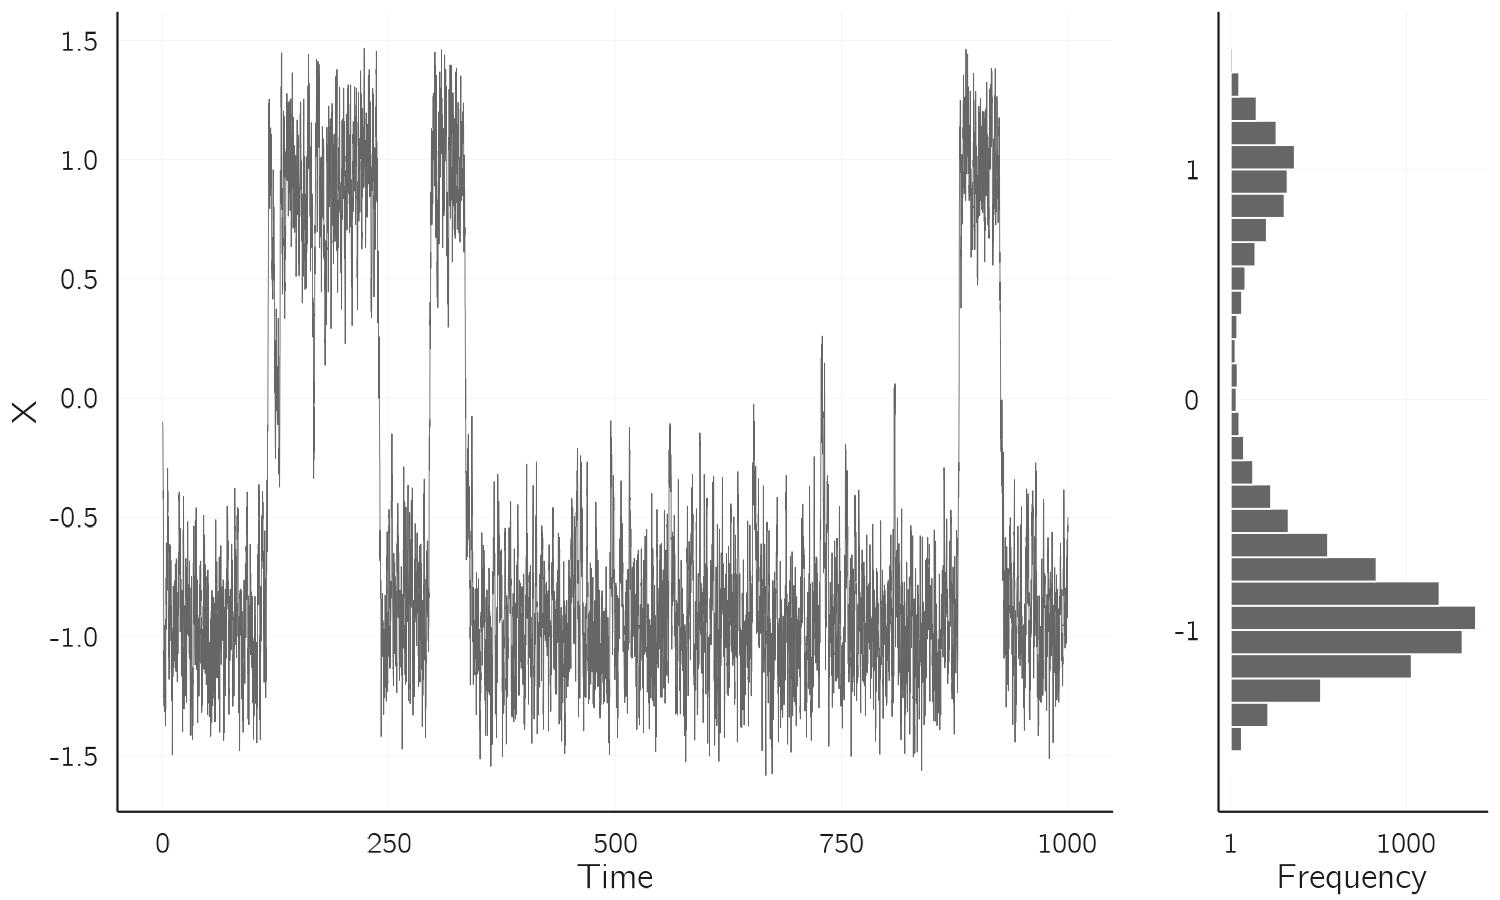
\includegraphics[width=9.375in,height=\textheight]{media/ch4n/fig-ch4n-img2-old-50.jpg}

}

\caption{\label{fig-ch4n-img2-old-50}Spontaneous jumps in the cusp due
to stochastics (noise). Due to stochastic perturbations, the system
occasionally jumps over the maxima that separate the minima.
Interestingly, when the noise is reduced, the time series tends to
become trapped in a single equilibrium. Conversely, increased noise
helps reveal the overall equilibrium landscape. This phenomenon is known
as stochastic resonance.}

\end{figure}%

\subsection{Bifurcation analysis}\label{sec-Bifurcation-analysis}

By combining the Grind functions \texttt{newton()} and
\texttt{continue()}, we can perform bifurcation analysis. The
\texttt{newton()} function finds stable and unstable fixed points, and
the \texttt{continue()} function implements the parameter continuation
of a steady state, providing a bifurcation diagram. It shows the change
in equilibria when we change a parameter. This is what we did in Chapter
2 for the logistic map, when we varied \(r\) and plotted the equilibria
(see figure~\ref{fig-ch2-img8}).

It is often necessary to run the combination of these two functions
repeatedly, starting from different initial states. The code to create
figure~\ref{fig-ch4n-img3-old-51} is:

\begin{Shaded}
\begin{Highlighting}[]
\NormalTok{p }\OtherTok{\textless{}{-}} \FunctionTok{c}\NormalTok{(}\AttributeTok{a=}\DecValTok{0}\NormalTok{,}\AttributeTok{b=}\DecValTok{1}\NormalTok{)}
\NormalTok{low }\OtherTok{\textless{}{-}} \FunctionTok{newton}\NormalTok{(}\AttributeTok{s=}\FunctionTok{c}\NormalTok{(}\AttributeTok{X=}\SpecialCharTok{{-}}\DecValTok{1}\NormalTok{)) }\CommentTok{\# finds a minimum starting from X = {-}1}
\CommentTok{\# Continue this steady state varying a}
\FunctionTok{continue}\NormalTok{(low,}\AttributeTok{x=}\StringTok{"a"}\NormalTok{,}\AttributeTok{y=}\StringTok{"X"}\NormalTok{,}\AttributeTok{xmin=}\SpecialCharTok{{-}}\DecValTok{2}\NormalTok{,}\AttributeTok{xmax=}\DecValTok{2}\NormalTok{,}\AttributeTok{ymax=}\DecValTok{2}\NormalTok{) }
\NormalTok{high }\OtherTok{\textless{}{-}} \FunctionTok{newton}\NormalTok{(}\AttributeTok{s=}\FunctionTok{c}\NormalTok{(}\AttributeTok{X=}\DecValTok{1}\NormalTok{)) }\CommentTok{\# again starting from X = 1}
\FunctionTok{continue}\NormalTok{(high,}\AttributeTok{x=}\StringTok{"a"}\NormalTok{,}\AttributeTok{y=}\StringTok{"X"}\NormalTok{,}\AttributeTok{xmin=}\SpecialCharTok{{-}}\DecValTok{2}\NormalTok{,}\AttributeTok{xmax=}\DecValTok{2}\NormalTok{,}\AttributeTok{ymax=}\DecValTok{2}\NormalTok{,}\AttributeTok{add=}\NormalTok{T)}
\end{Highlighting}
\end{Shaded}

\begin{figure}

\centering{

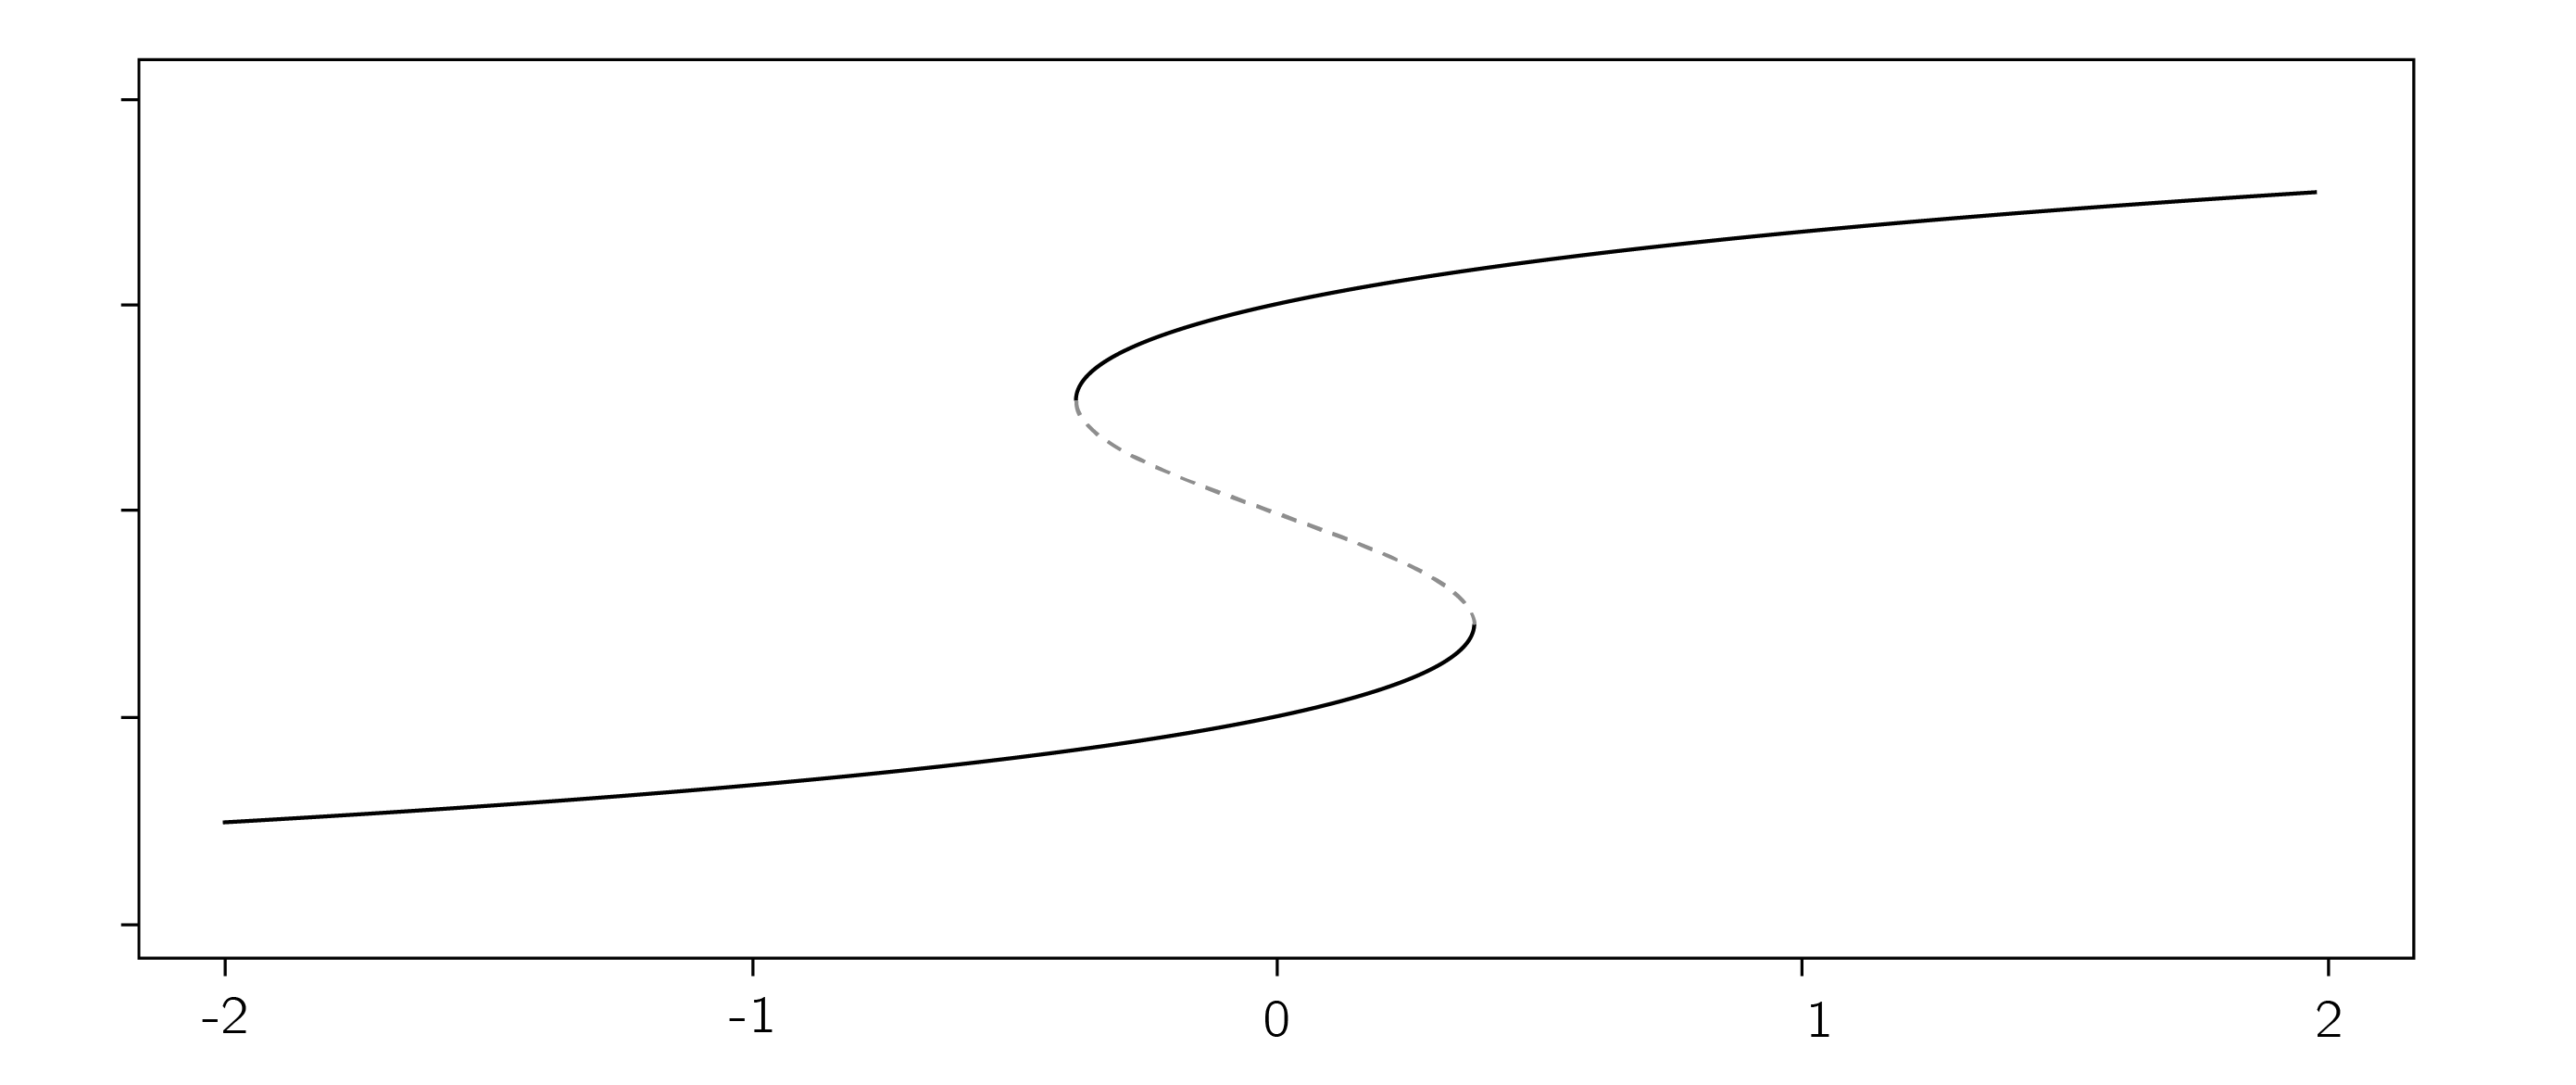
\includegraphics{media/ch4n/ch4n-2__figure51.png}

}

\caption{\label{fig-ch4n-img3-old-51}Hysteresis plot made with
\texttt{newton()} and \texttt{continue()}. The function
\texttt{newton()} finds an equilibrium, which is used in
\texttt{continue()} to vary the normal variable a until a bifurcation
point is found.}

\end{figure}%

Another great tool in R is the deBif package by de Roos.\footnote{\url{https://cran.r-project.org/web/packages/deBif/deBif.pdf}}
This is an R Shiny application that uses the same model specification
and allows for a more interactive investigation. Given our previous
model and the definition of \(s\) and \(p\), we can run:

\begin{Shaded}
\begin{Highlighting}[]
\FunctionTok{install.packages}\NormalTok{(}\StringTok{"deBif"}\NormalTok{)}
\FunctionTok{library}\NormalTok{(deBif)}
\FunctionTok{phaseplane}\NormalTok{(model,s,p)}
\end{Highlighting}
\end{Shaded}

The \texttt{phaseplane()} function returns a time plot and the steady
states. You can change parameters and initial states on the left side,
and plot parameters on the upper right side (click on the two gears).
The Steady States option is very useful as it shows the stable and
unstable fixed points. Make sure that the minima and maxima of the plot
axes are set correctly.

With

\begin{Shaded}
\begin{Highlighting}[]
\FunctionTok{bifurcation}\NormalTok{(model,s,p)}
\end{Highlighting}
\end{Shaded}

You can create one- and two-parameter bifurcation diagrams (using the LP
curve option, see figure~\ref{fig-ch4n-img4-old-52}). The two-parameter
bifurcation diagram (bottom left) cannot be created in Grind. See the
deBif help pages (with \texttt{??deBif}) for further instructions.

\begin{figure}

\centering{

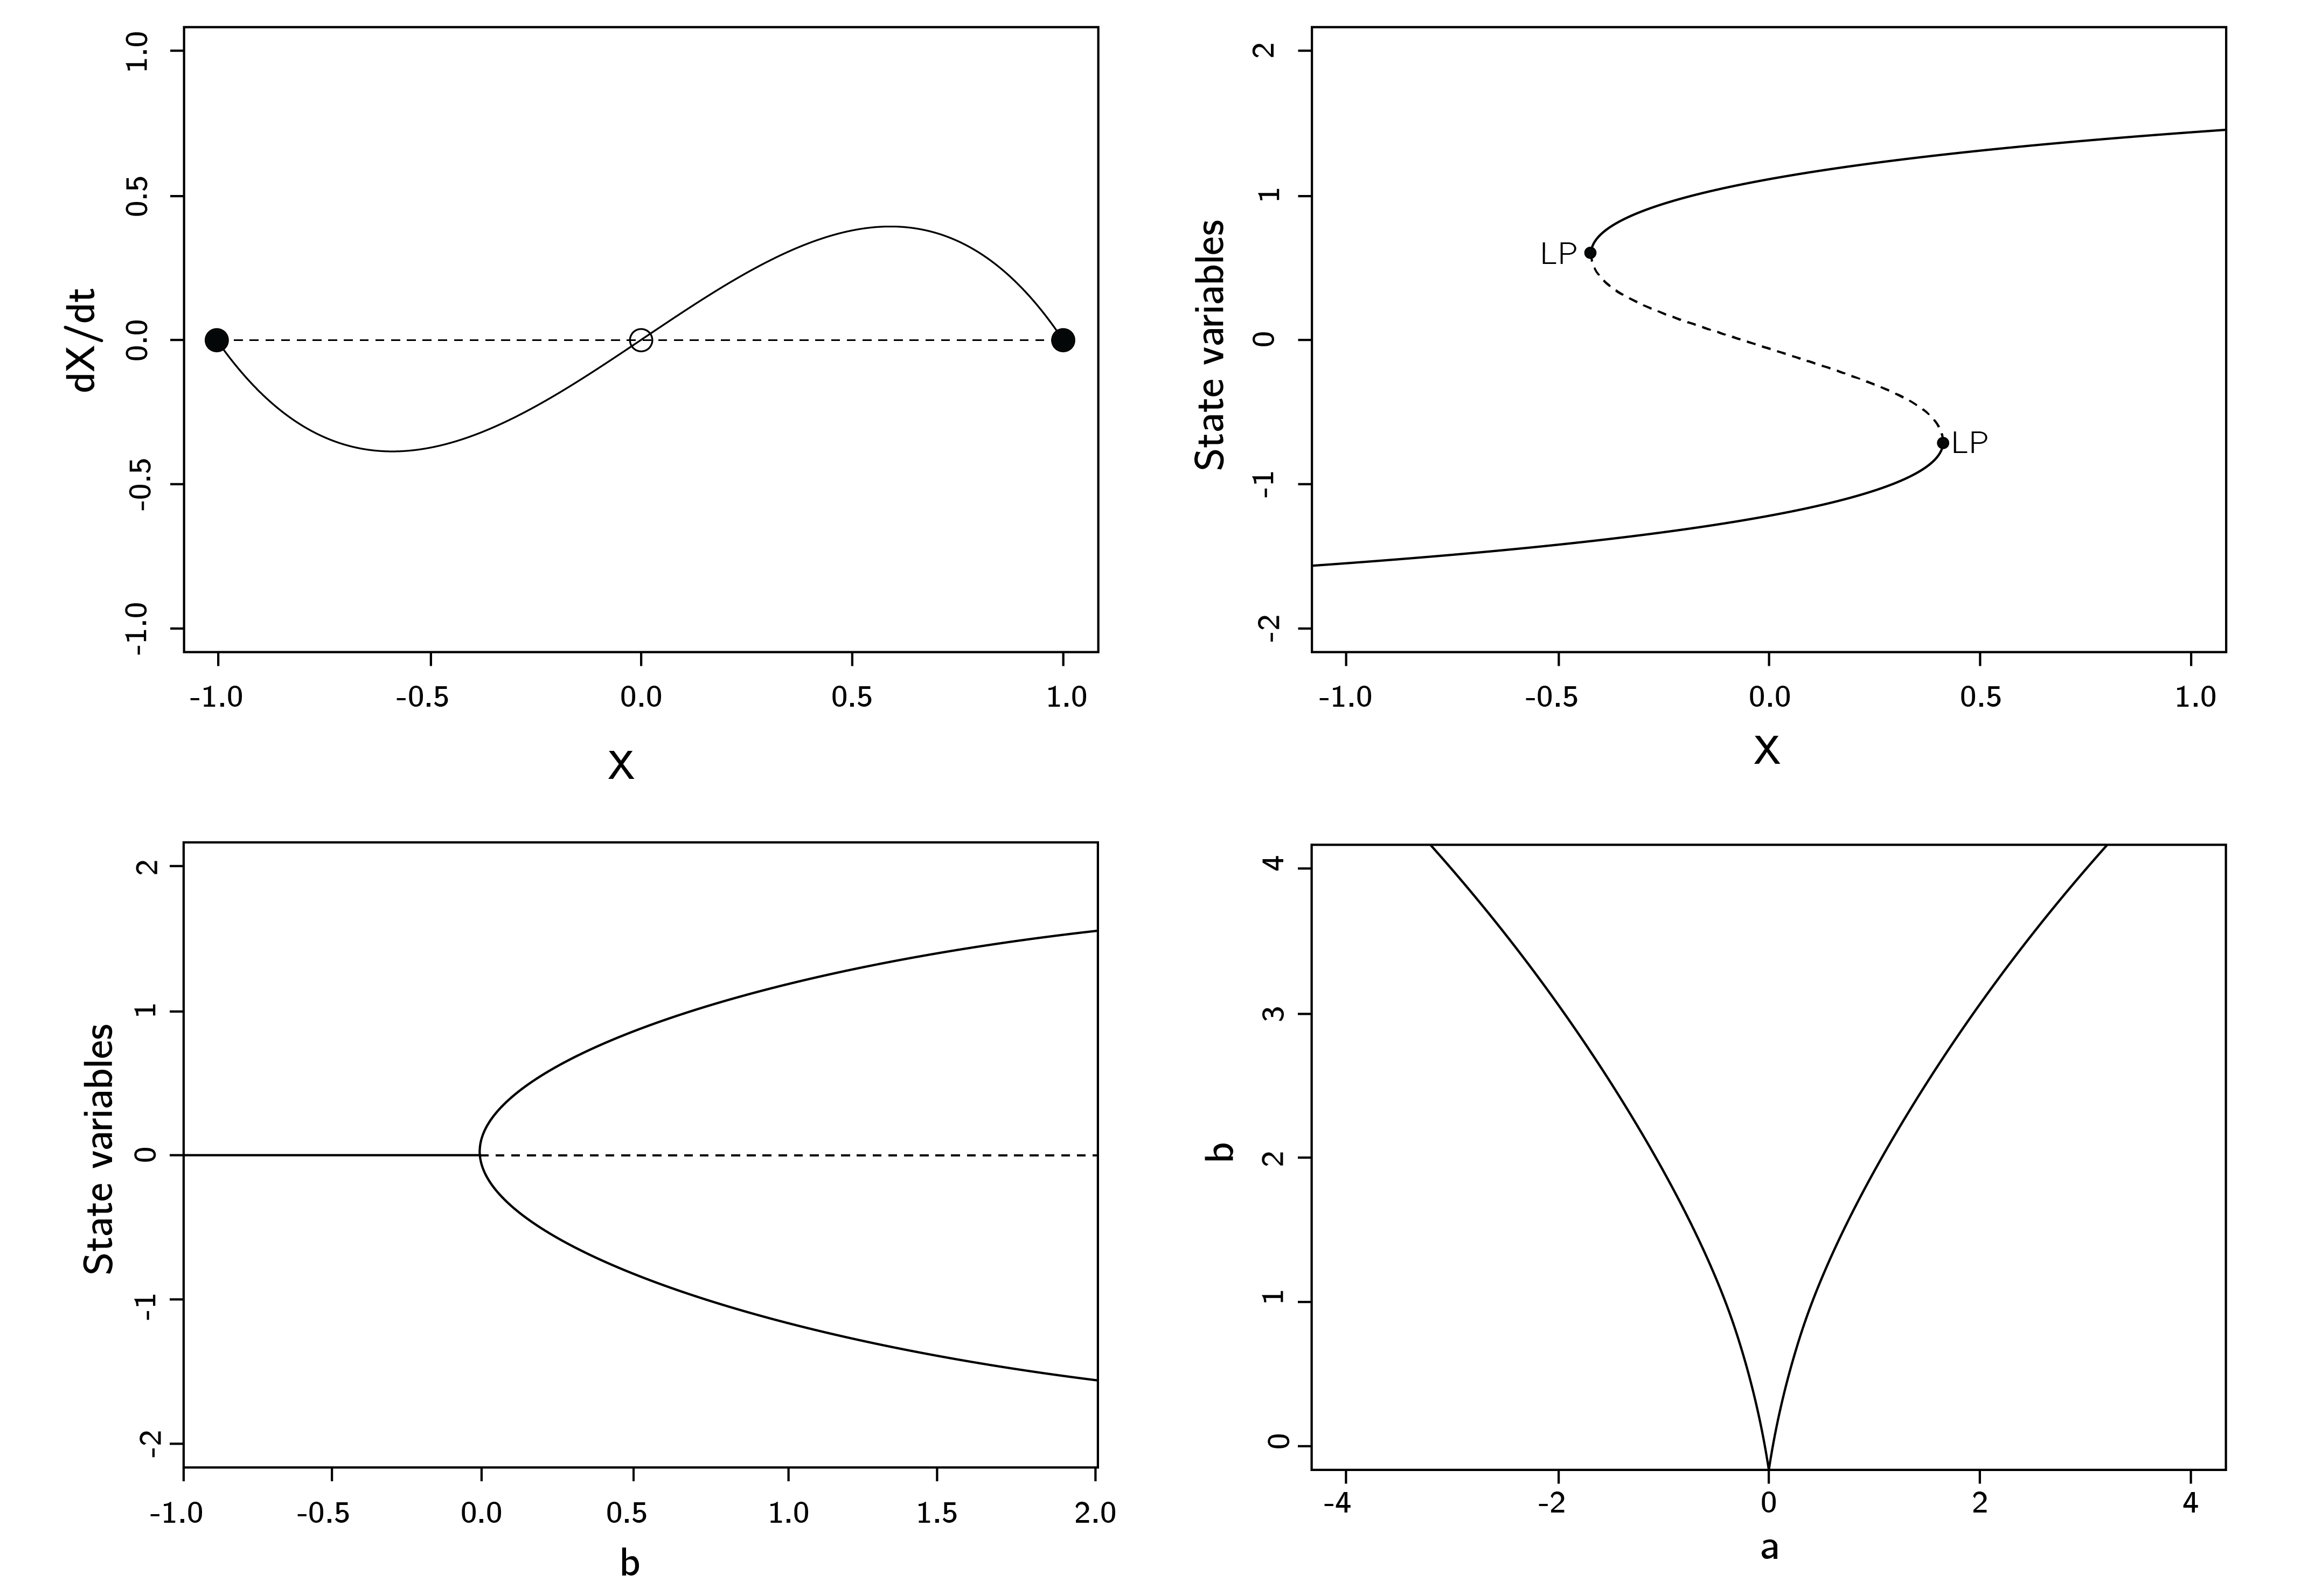
\includegraphics{media/ch4n/ch4n-4__figure53.png}

}

\caption{\label{fig-ch4n-img4-old-52}Output from Shiny app deBif. The
last plot is a two-dimensional bifurcation diagram showing the
bifurcation lines of the cusp in the \(a\), \(b\) plane. This plot
cannot be made with Grind.}

\end{figure}%

\subsection{Spruce budworm outbreak
model}\label{sec-Spruce-Budworm-outbreak-model}

In Chapter 3, section~\ref{sec-Mechanistic-models}, I introduced the
spruce budworm outbreak model. We will use this model later as a model
of addiction. The bifurcation diagram can be made with:

\begin{Shaded}
\begin{Highlighting}[]
\NormalTok{spruce }\OtherTok{\textless{}{-}} \ControlFlowTok{function}\NormalTok{(t, state, parms) \{}
  \FunctionTok{with}\NormalTok{(}\FunctionTok{as.list}\NormalTok{(}\FunctionTok{c}\NormalTok{(state,parms)), \{}
\NormalTok{    du }\OtherTok{=}\NormalTok{ r}\SpecialCharTok{*}\NormalTok{u}\SpecialCharTok{*}\NormalTok{(}\DecValTok{1} \SpecialCharTok{{-}}\NormalTok{ u}\SpecialCharTok{/}\NormalTok{q)}\SpecialCharTok{{-}}\NormalTok{u}\SpecialCharTok{\^{}}\DecValTok{2}\SpecialCharTok{/}\NormalTok{(}\DecValTok{1}\SpecialCharTok{+}\NormalTok{u}\SpecialCharTok{\^{}}\DecValTok{2}\NormalTok{)}
    \FunctionTok{return}\NormalTok{(}\FunctionTok{list}\NormalTok{(}\FunctionTok{c}\NormalTok{(du)))}
\NormalTok{  \})}
\NormalTok{\}}
\NormalTok{state }\OtherTok{\textless{}{-}} \FunctionTok{c}\NormalTok{(}\AttributeTok{u =} \FloatTok{0.5}\NormalTok{)}
\NormalTok{parms }\OtherTok{\textless{}{-}} \FunctionTok{c}\NormalTok{(}\AttributeTok{r =} \FloatTok{0.4}\NormalTok{, }\AttributeTok{q =} \DecValTok{10}\NormalTok{)}
\FunctionTok{bifurcation}\NormalTok{(spruce, state, parms)}
\end{Highlighting}
\end{Shaded}

Note that this predator-prey model consists of only one equation. There
is no separate dynamic equation for the birds. The reason is that these
budworm outbreaks happen in a few weeks. Birds do not reproduce on this
time scale. The variables are reparametrized (see
section~\ref{sec-Mechanistic-models}). The predation term, in the
original parametrization \(- BN^{2}/(A^{2} + N^{2})\), also has a
logistic form that starts to accelerate at \(N = A\) up to the maximum
level \(B\). The slow start \(A\) is used because birds only switch
their diet to budworms when this population reaches a certain level
(Ludwig, Jones, and Holling 1978). The fixed number of birds can only
eat \(B\) budworms. This specific predation term is called the Holling
type III model. All Holling types and their formulas are shown in
figure~\ref{fig-ch4n-img5-old-53}.

\begin{figure}

\centering{

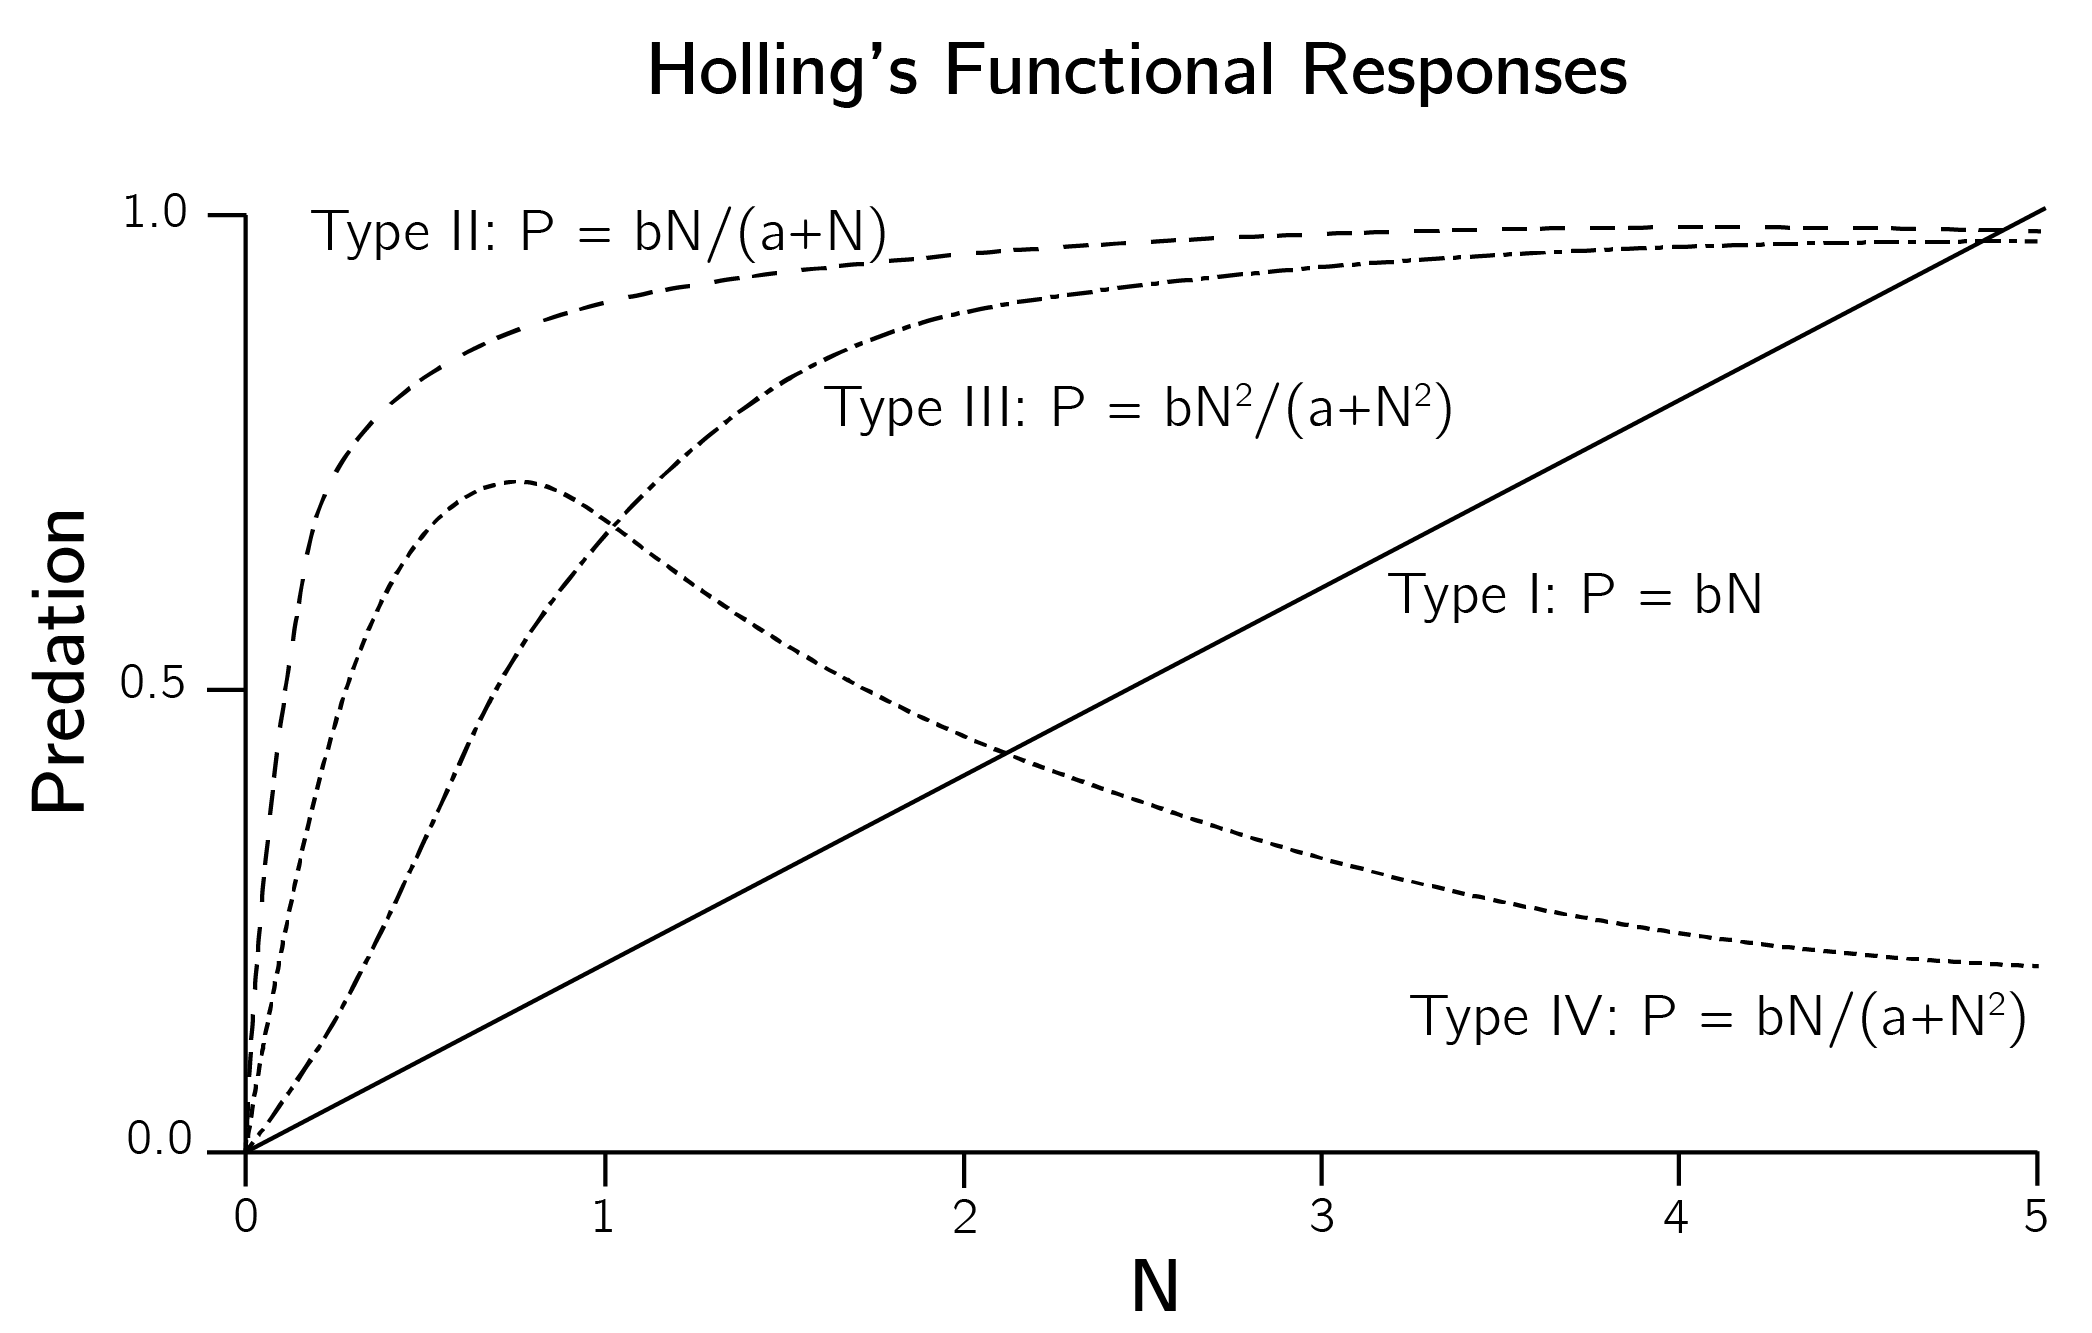
\includegraphics{media/ch4n/ch4-5-may31.png}

}

\caption{\label{fig-ch4n-img5-old-53}The Holling functional response
models. Type III is used in the spruce budworm model.}

\end{figure}%

\subsection{Evaluation of ecological
modeling}\label{sec-Evaluation-of-ecological-modelling}

Understanding the technical basics of dynamical systems theory is one
thing, but actually building useful dynamical system models is quite
another. Every term in each differential equation of a model needs some
underpinning. These models make many assumptions, both implicit and
explicit. The Lotka---Volterra model, for example, assumes that the prey
population grows exponentially in the absence of the predator, that the
predator population dies off with the prey population and does not
switch to other prey species, that the response of the predator
population to changes in the prey population is direct and not delayed,
that there is no spatial component to the model, and that the rates of
change of the populations are proportional to their sizes, to name just
a few. These assumptions are widely debated in the biological literature
(Abrams et al. 2000), and modifying these assumptions may have
significant consequences. {\marginnote{\begin{footnotesize}Hundreds of
extensions and variants of the
Lotka\end{footnotesize}}}---{\marginnote{\begin{footnotesize}Volterra
model have been proposed and studied.\end{footnotesize}}}

For example, the original Lotka---Volterra model has no stable points,
only limit cycles. While these cycles have been observed in nature, they
are not overwhelmingly common. As we have seen, the dynamics of the
system are significantly altered when prey growth is made dependent on
prey density. This model has fixed-point equilibria instead of limit
cycles.

Adding a spatial component can also make a big difference, as shown in
the example of hypercycles in see section~\ref{sec-Biology} (see
Szostak, Wasik, and Blazewicz (2016) for a brief review). Adding more
prey and predator species also makes a difference (Johnson, Mumma, and
St-Laurent 2019). There are many interesting options for the predator
term in the prey equation. Tyutyunov and Titova (2020) compare 12
trophic functions, alternatives to the Holling functional responses. The
options are overwhelming. Biologists face a problem here that I
discussed in Chapter 1, section~\ref{sec-The-art-of-simplification}.
Models easily become too complex. Recall that the traffic simulation
models were extremely simple, yet sufficient to explain key phenomena.

An additional problem is that empirically testing all these different
models is difficult. Although the quality of biological data is often
superior to that of psychological data, biologists must also rely on the
qualitative predictions of their models. Models in chemistry and
especially physics can often be tested quantitatively. Transitions occur
precisely at the predicted values of the control variables. Ecological
models, much like those in psychology, do not allow for this level of
prediction. This is a problem because if we can only test our model
qualitatively (Are there limit cycles? What type of transitions can be
detected? Is there hysteresis?), many model choices are not particularly
relevant. {\marginnote{\begin{footnotesize}One of the most significant
challenges in complex-systems research in the life sciences and
psychology is constructing dynamical system models that effectively
address these data-related issues.\end{footnotesize}}}

A case in which this is less of an issue is the traffic example that I
introduced in Chapter 1. I asked you to play around with the online
simulation. We now know the basics to better understand this model. The
Wikipedia page on this model (Intelligent Driver Model) presents the
equations, which are also coupled ordinary differential equations. The
implementation in Grind of the simplest case looks like this:

\begin{Shaded}
\begin{Highlighting}[]
\NormalTok{model }\OtherTok{\textless{}{-}} \ControlFlowTok{function}\NormalTok{(t, state, parms)\{}
  \FunctionTok{with}\NormalTok{(}\FunctionTok{as.list}\NormalTok{(}\FunctionTok{c}\NormalTok{(state,parms)),\{}
\NormalTok{    x }\OtherTok{\textless{}{-}}\NormalTok{ state[}\DecValTok{1}\SpecialCharTok{:}\NormalTok{n]}
\NormalTok{    v }\OtherTok{\textless{}{-}}\NormalTok{ state[(n}\SpecialCharTok{+}\DecValTok{1}\NormalTok{)}\SpecialCharTok{:}\NormalTok{(}\DecValTok{2}\SpecialCharTok{*}\NormalTok{n)]}
\NormalTok{    dx }\OtherTok{\textless{}{-}}\NormalTok{  v }\CommentTok{\# change in distance = speed}
\NormalTok{    delta\_v }\OtherTok{\textless{}{-}}\NormalTok{ v}\SpecialCharTok{{-}}\NormalTok{ m }\SpecialCharTok{\%*\%}\NormalTok{ v }\CommentTok{\# difference in speed to next car}
\NormalTok{    s\_alpha }\OtherTok{\textless{}{-}}\NormalTok{ m }\SpecialCharTok{\%*\%}\NormalTok{ x }\SpecialCharTok{{-}}\NormalTok{ x }\SpecialCharTok{{-}}\NormalTok{l }\CommentTok{\#  distance to next car}
\NormalTok{    s\_alpha[n] }\OtherTok{\textless{}{-}} \DecValTok{100} \CommentTok{\# front car has no car in front}
\NormalTok{    s\_star }\OtherTok{\textless{}{-}}\NormalTok{ s0 }\SpecialCharTok{+}\NormalTok{ v }\SpecialCharTok{*}\NormalTok{ T }\SpecialCharTok{+}\NormalTok{ v }\SpecialCharTok{*}\NormalTok{ delta\_v }\SpecialCharTok{/}\NormalTok{ (}\DecValTok{2}\SpecialCharTok{*}\FunctionTok{sqrt}\NormalTok{(a}\SpecialCharTok{*}\NormalTok{b))}
\NormalTok{    dv }\OtherTok{\textless{}{-}}\NormalTok{ a }\SpecialCharTok{*}\NormalTok{ (}\DecValTok{1} \SpecialCharTok{{-}}\NormalTok{ (v}\SpecialCharTok{/}\NormalTok{v0)}\SpecialCharTok{\^{}}\NormalTok{delta }\SpecialCharTok{{-}}\NormalTok{ (s\_star}\SpecialCharTok{/}\NormalTok{s\_alpha)}\SpecialCharTok{\^{}}\DecValTok{2}\NormalTok{) }\CommentTok{\# change in speed}
    \FunctionTok{return}\NormalTok{(}\FunctionTok{list}\NormalTok{(}\FunctionTok{c}\NormalTok{(dx,dv)))}
\NormalTok{  \})}
\NormalTok{\}}

\NormalTok{n}\OtherTok{=}\DecValTok{50}
\NormalTok{p }\OtherTok{\textless{}{-}} \FunctionTok{c}\NormalTok{(}\AttributeTok{l=}\DecValTok{5}\NormalTok{,}\AttributeTok{v0=}\DecValTok{30}\NormalTok{,}\AttributeTok{T=}\FloatTok{1.5}\NormalTok{,}\AttributeTok{a=}\NormalTok{.}\DecValTok{73}\NormalTok{,}\AttributeTok{b=}\FloatTok{1.67}\NormalTok{,}\AttributeTok{delta=}\DecValTok{4}\NormalTok{,}\AttributeTok{s0=}\DecValTok{2}\NormalTok{)}
\NormalTok{x\_init }\OtherTok{\textless{}{-}}\NormalTok{ (}\DecValTok{0}\SpecialCharTok{:}\NormalTok{(n}\DecValTok{{-}1}\NormalTok{))}\SpecialCharTok{*}\NormalTok{(p[}\StringTok{\textquotesingle{}s0\textquotesingle{}}\NormalTok{]}\SpecialCharTok{+}\NormalTok{p[}\StringTok{\textquotesingle{}l\textquotesingle{}}\NormalTok{])}
\NormalTok{v\_init }\OtherTok{\textless{}{-}} \FunctionTok{rep}\NormalTok{(}\DecValTok{0}\NormalTok{,n)}
\NormalTok{s }\OtherTok{\textless{}{-}} \FunctionTok{c}\NormalTok{(x\_init,v\_init)}

\NormalTok{m }\OtherTok{\textless{}{-}} \FunctionTok{diag}\NormalTok{(}\DecValTok{1}\NormalTok{, n, n); m}\OtherTok{=} \FunctionTok{rbind}\NormalTok{(m[}\SpecialCharTok{{-}}\DecValTok{1}\NormalTok{,],}\DecValTok{0}\NormalTok{) }\CommentTok{\# order cars}
\CommentTok{\# simulation with front car suddenly breaking at t = 150}
\NormalTok{data}\OtherTok{=}\FunctionTok{run}\NormalTok{(}\AttributeTok{tmax=}\DecValTok{300}\NormalTok{,}\AttributeTok{timeplot =}\NormalTok{ F,}\AttributeTok{table=}\NormalTok{T,}\AttributeTok{after =} \StringTok{\textquotesingle{}if (t==150) state[2*n] = 0\textquotesingle{}}\NormalTok{)}
\FunctionTok{matplot}\NormalTok{(data[,}\DecValTok{2}\SpecialCharTok{:}\NormalTok{(n}\SpecialCharTok{+}\DecValTok{1}\NormalTok{)],}\AttributeTok{type=}\StringTok{\textquotesingle{}l\textquotesingle{}}\NormalTok{,}\AttributeTok{bty=}\StringTok{\textquotesingle{}n\textquotesingle{}}\NormalTok{,}\AttributeTok{xlab=}\StringTok{\textquotesingle{}time\textquotesingle{}}\NormalTok{,}\AttributeTok{ylab =} \StringTok{\textquotesingle{}x\textquotesingle{}}\NormalTok{)}
\end{Highlighting}
\end{Shaded}

\begin{figure}

\centering{

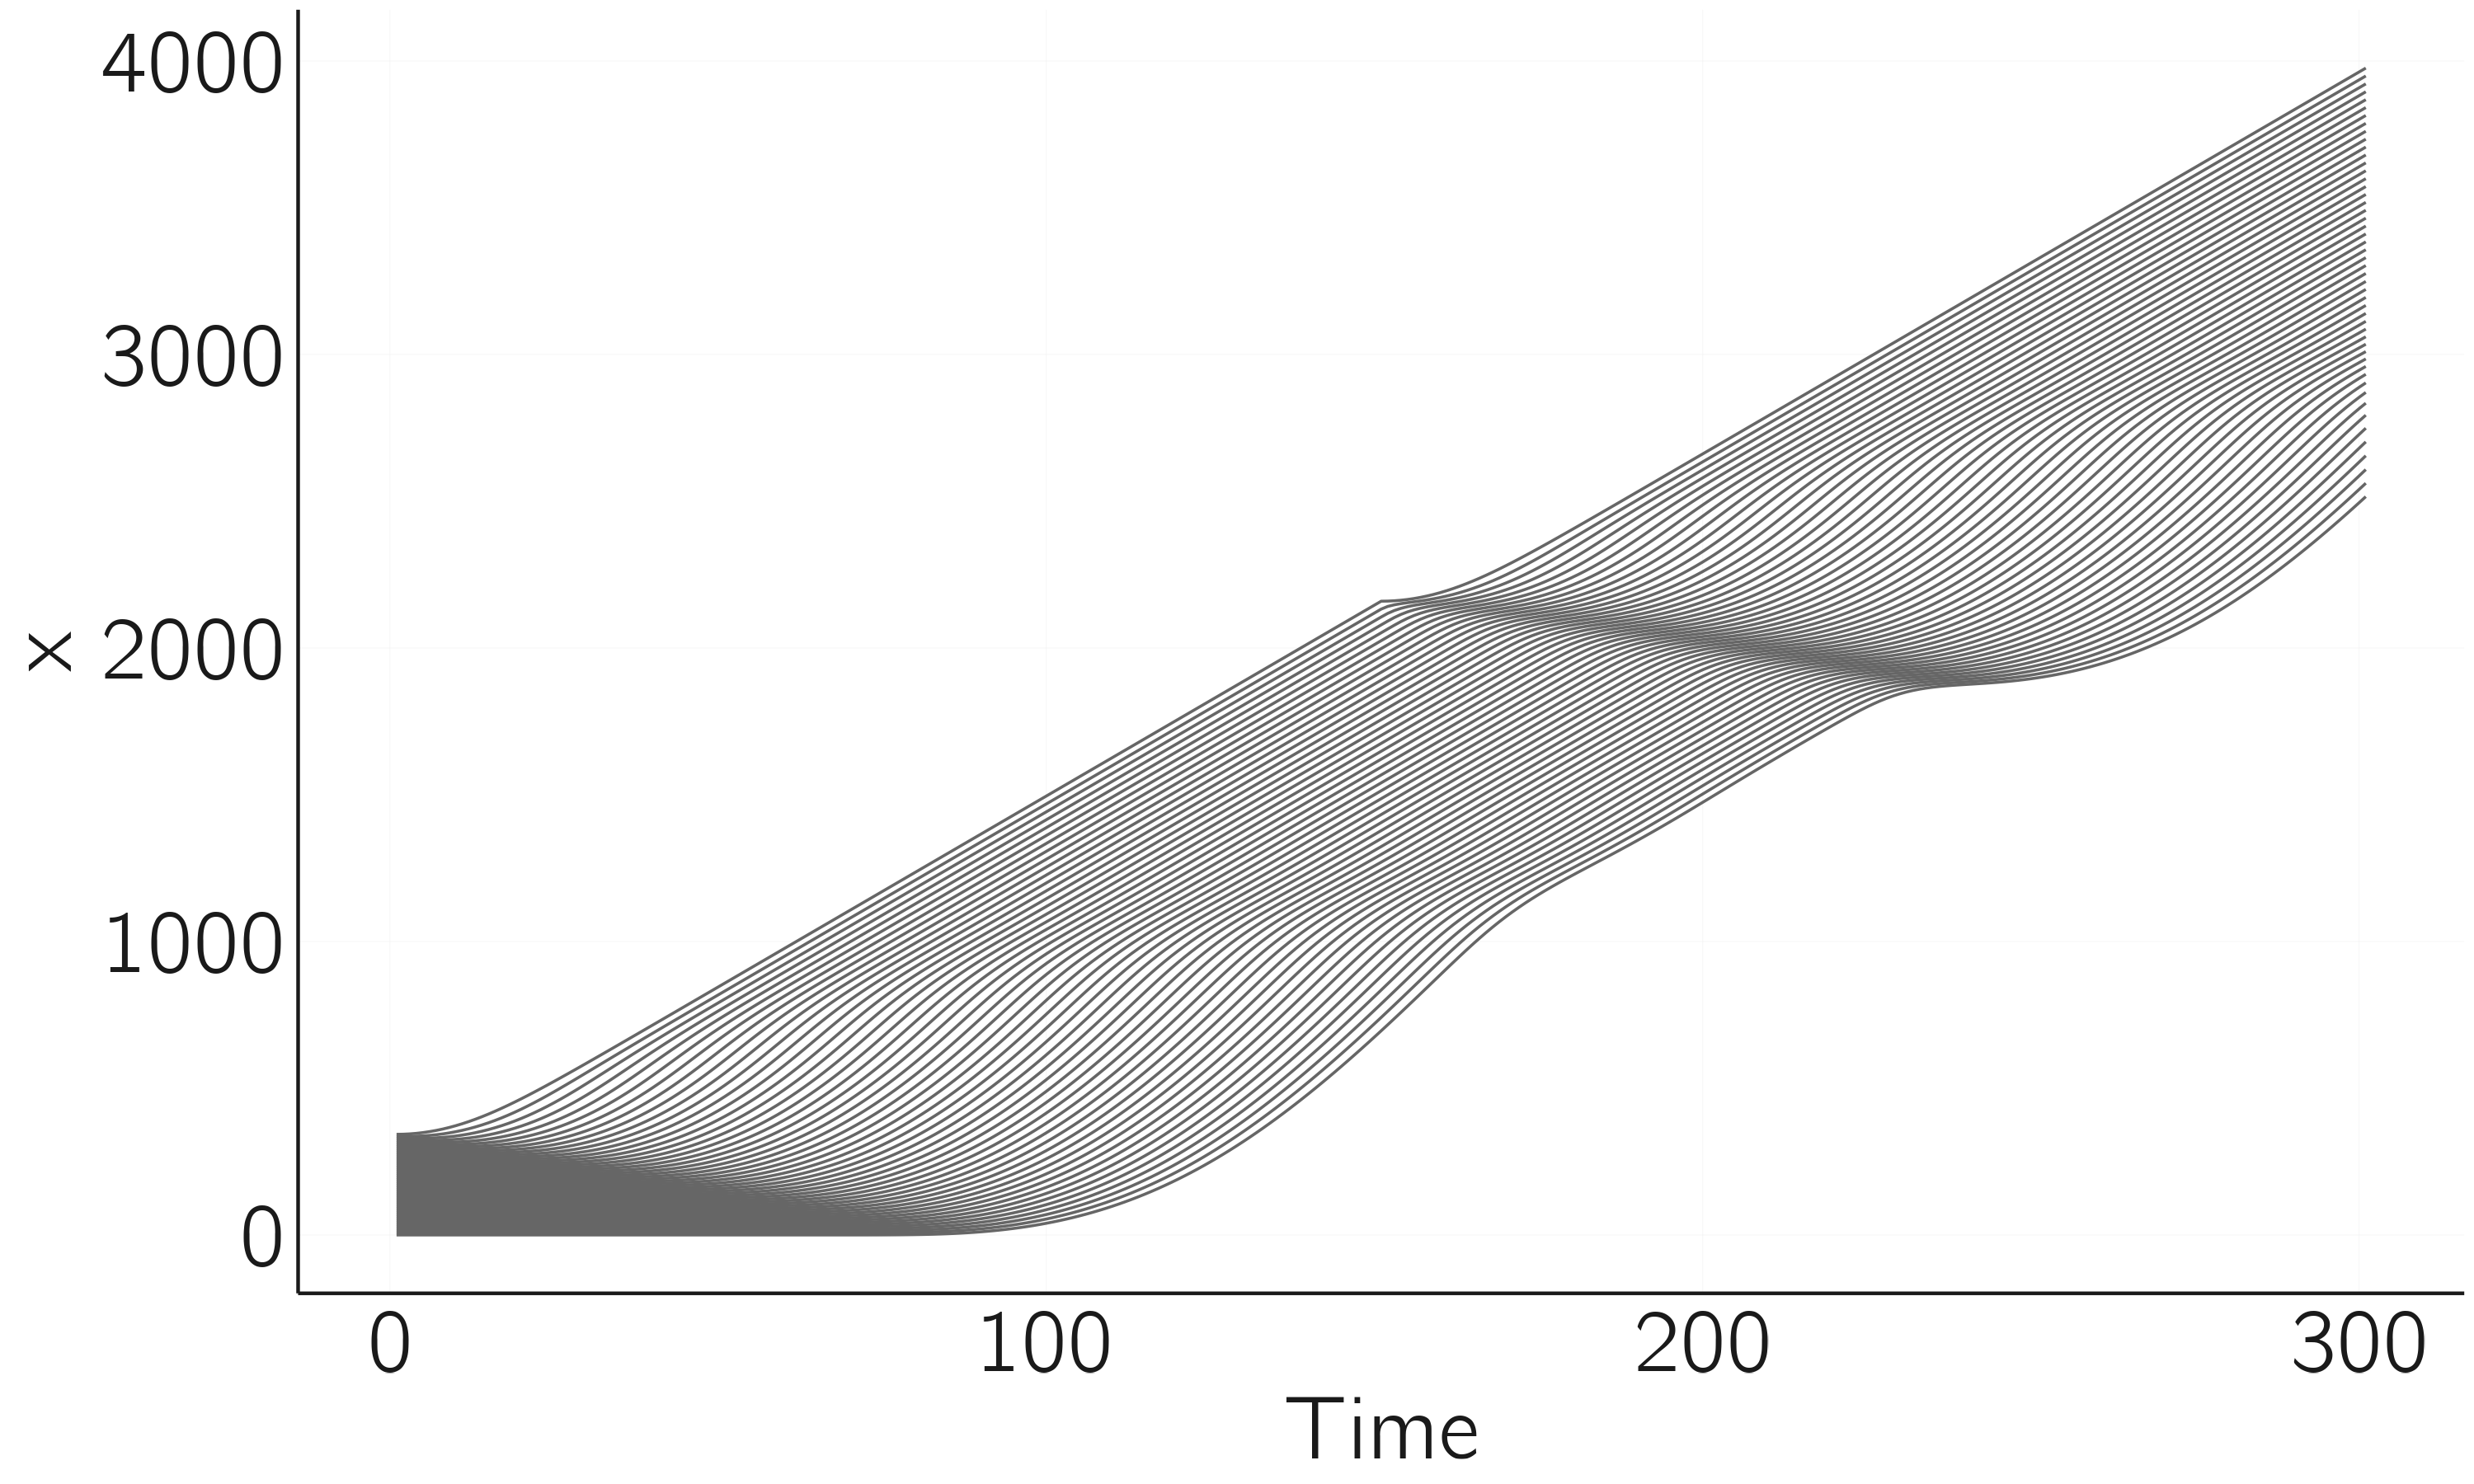
\includegraphics{media/ch4n/fig-ch4n-img6-old-54.png}

}

\caption{\label{fig-ch4n-img6-old-54}The traffic jam simulation. The top
line represents the front car, which moves off immediately. Other cars
are waiting for their turn. At \(t = 150\), the first car suddenly
breaks off, creating a traffic jam for the later cars. The effect of
this disturbance is greater for the last car than for the first car.
This simulated graph resembles the real data very well (see for example
figure 9 in Jusup et al. 2022).}

\end{figure}%

The result of this simulation is shown in
figure~\ref{fig-ch4n-img6-old-54}. Understanding the reasoning behind
the differential equation is not so easy, but I want to make another
point. The Wikipedia page gives parameters values with units (s, m/s, or
m/s\textsuperscript{2}). One can also have dimension-free parameters
(the acceleration exponent).
{\marginnote{\begin{footnotesize}Dimensional analysis involves analyzing
the dimensions of quantities to derive relationships and scaling laws,
ensuring that the equations are consistent.\end{footnotesize}}} This
dimensional analysis is a crucial step in modeling in physics but a weak
point in biological and especially psychological applications. This
hampers the quantitative test of models.

\section{Psychological models}\label{sec-Psychological-models}

In this section, I present an overview of dynamical systems models in
psychology, primarily in the form of systems of differential equations.
Although the list is extensive, it is not exhaustive. It is important to
explore different models and applications before embarking on your own
modeling efforts.

\subsection{Response time models}\label{sec-Response-time-models}

Many dynamic models have been proposed in the study of speeded
decision-making (Bogacz et al. 2006). The best-studied case is the
two-alternative forced-choice task, where a stimulus is presented, and a
choice must be made between two alternatives as quickly as possible. The
stimulus could be an arrow pointing left or right. Most popular are
accumulator models (figure~\ref{fig-ch4n-img7-old-55}).
{\marginnote{\begin{footnotesize}Accumulator models assume that noisy
information is accumulated over time until a decision bound is reached
and a motor response is initiated.\end{footnotesize}}}

\begin{figure}

\centering{

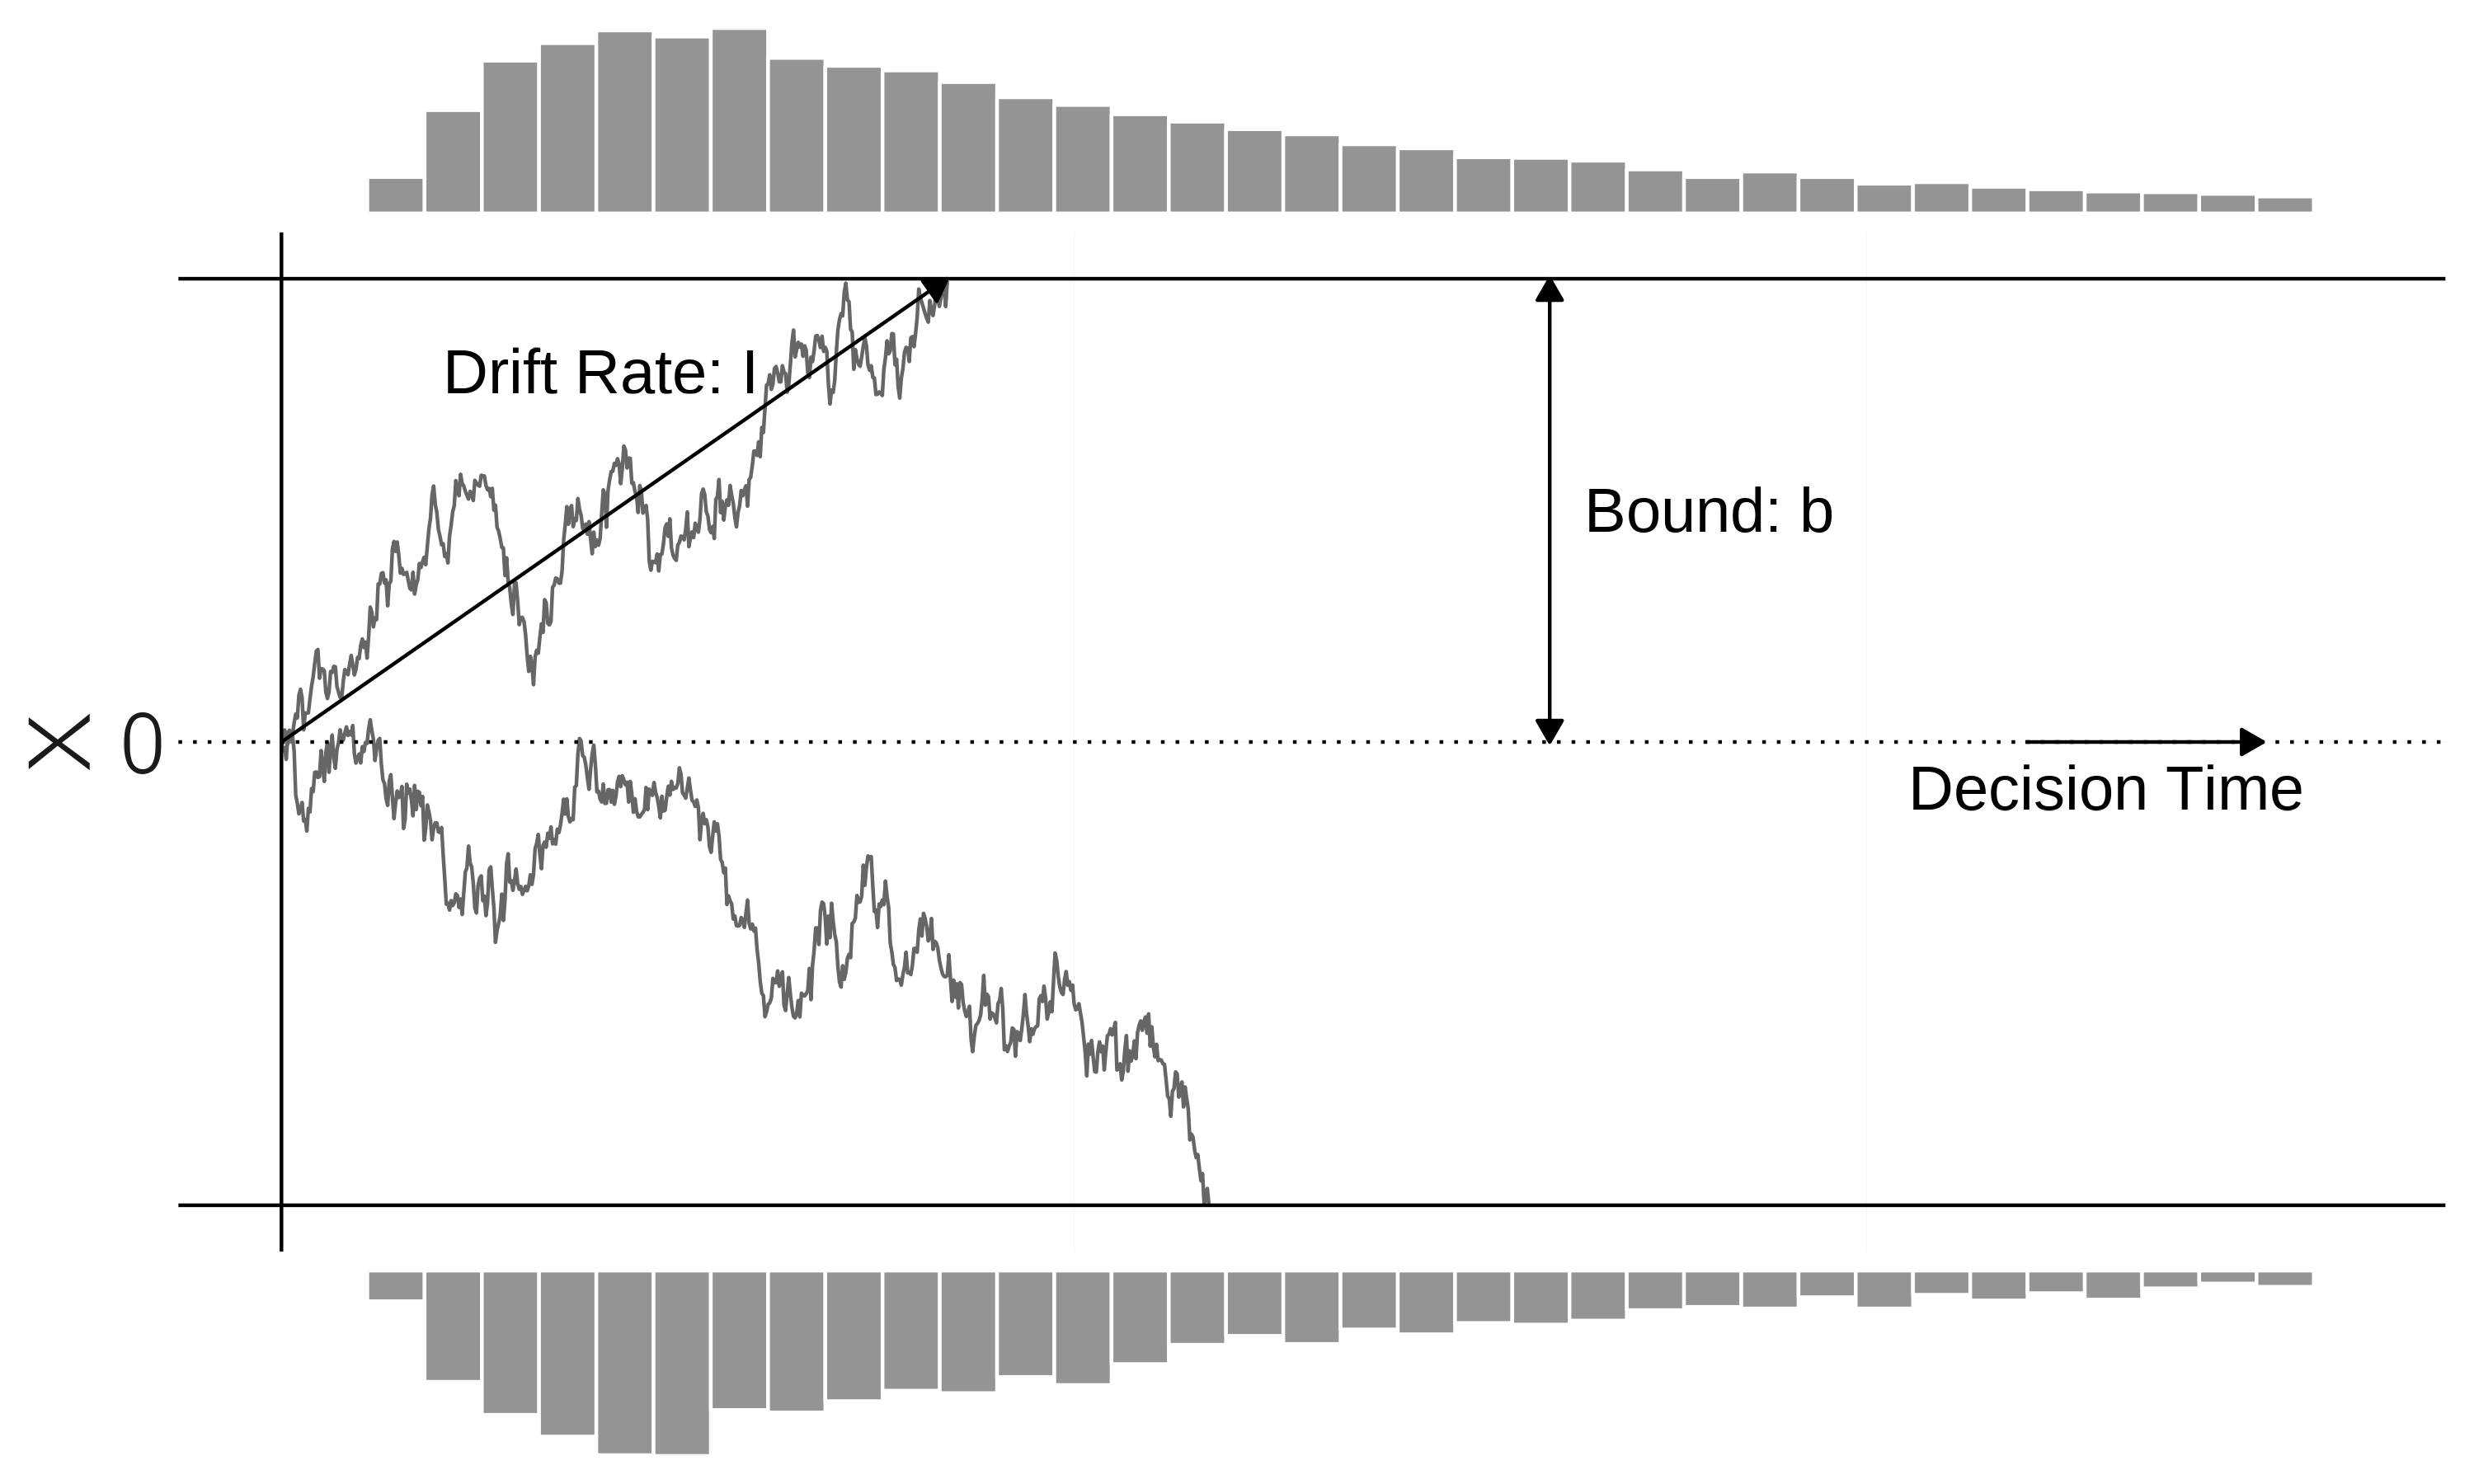
\includegraphics[width=8.33333in,height=\textheight]{media/ch4n/fig-ch4n-img7-old-55.png}

}

\caption{\label{fig-ch4n-img7-old-55}A stochastic accumulator model of
speeded decision-making. Evidence accumulates in stochastic steps biased
by the drift rate \(I\) (stimulus related). When one of the bounds is
reached, a response is generated that may be incorrect if the bounds are
too low.}

\end{figure}%

One way to model this process is with a single stochastic linear
differential equation, called the drift-diffusion model (DDM), with
\(I\) as the stimulus-driven input:

\begin{equation}\phantomsection\label{eq-ch4n-6-old-26}{
dX = Idt + \sigma dW
}\end{equation}

As before, \(dt\) is moved to the left-hand side of the equation. \(dW\)
is white noise, normally distributed with 0 mean and with standard
deviation \(\sigma\) (set to .1 by default). We start at 0,
\(X_{t = 0} = 0\), assuming no bias for one of the choice alternatives.

The implementation of the model in Grind is quite simple. The trick is
again in the run statement, which adds white noise after each
step.\footnote{Simulating this model correctly is more difficult than
  one might expect. I refer to Tuerlinckx et al. (2001) for a discussion
  of methods.} We stop the run when either the negative or positive
bound is reached.

\begin{Shaded}
\begin{Highlighting}[]
\NormalTok{model }\OtherTok{\textless{}{-}} \ControlFlowTok{function}\NormalTok{(t, state, parms) \{}
  \FunctionTok{with}\NormalTok{(}\FunctionTok{as.list}\NormalTok{(}\FunctionTok{c}\NormalTok{(state,parms)), \{}
\NormalTok{    dX }\OtherTok{=}\NormalTok{ I}
    \FunctionTok{return}\NormalTok{(}\FunctionTok{list}\NormalTok{(}\FunctionTok{c}\NormalTok{(dX)))}
\NormalTok{  \})}
\NormalTok{\}}
\NormalTok{p }\OtherTok{\textless{}{-}} \FunctionTok{c}\NormalTok{(}\AttributeTok{I=}\NormalTok{.}\DecValTok{01}\NormalTok{); s }\OtherTok{\textless{}{-}} \FunctionTok{c}\NormalTok{(}\AttributeTok{X=}\DecValTok{0}\NormalTok{)}
\NormalTok{bound }\OtherTok{\textless{}{-}} \DecValTok{1}
\FunctionTok{run}\NormalTok{(}\AttributeTok{table=}\NormalTok{T,}\AttributeTok{method=}\StringTok{\textquotesingle{}euler\textquotesingle{}}\NormalTok{, }\AttributeTok{tstep=}\NormalTok{.}\DecValTok{1}\NormalTok{,}
    \AttributeTok{tmax=}\DecValTok{500}\NormalTok{,}\AttributeTok{after=}\StringTok{"state\textless{}{-}state+rnorm(1,mean=0,sd=0.1)*sqrt(tstep);}
\StringTok{    if(abs(state)\textgreater{}bound) break"}\NormalTok{,}\AttributeTok{ymin=}\SpecialCharTok{{-}}\NormalTok{bound,}\AttributeTok{ymax=}\NormalTok{bound)}
\end{Highlighting}
\end{Shaded}

The model explains observed response time and accuracy in terms of the
underlying process parameters, drift rate, and confidence bound. By
fitting the model to the data, we can determine whether slow responses
are due to a low drift rate (low skill or difficult task) or a
conservatively chosen bound.
{\marginnote{\begin{footnotesize}Accumulator models such as the
drift-diffusion model explain the speed-accuracy trade-off. If we set
our confidence bound higher, we are slower but more
accurate.\end{footnotesize}}}

A well-known extension of the drift-diffusion model is the
Ornstein---Uhlenbeck model:

\begin{equation}\phantomsection\label{eq-ch4n-7-old-27}{
dX = (\lambda x + I)dt + \sigma dW
}\end{equation}

For \(\lambda < 0\) this process converges to \(I/\lambda\) (assuming
\(\sigma = 0\)), while for \(\lambda > 0\) it diverges. For the
psychological interpretation, I refer to Bogacz et al. (2006). The
simplest two-dimensional model is the race model:

\begin{equation}\phantomsection\label{eq-ch4n-8-old-28}{
\begin{gathered}
dX_{1} = I_{1}dt + \sigma W_{1} \\
dX_{2} = I_{2}dt + \sigma W_{2} 
\end{gathered}
}\end{equation}

Now two independent processes run (race) to one positive bound. The
first one to arrive wins. More biologically inspired models involve
inhibition. The equations of mutual inhibition model are:

\begin{equation}\phantomsection\label{eq-ch4n-9-old-29}{
\begin{gathered}
dX_{1} = (-k_{1}X_{1} - w_{1}X_{2} + I_{1})dt + \sigma W_{1} \\
dX_{2} = (-k_{2}X_{2} - w_{2}X_{1} + I_{2})dt + \sigma W_{2}
\end{gathered}
}\end{equation}

Note that these are all linear dynamical systems that do not exhibit
complex behavior. Examples of nonlinear alternatives are presented in
Roxin and Ledberg (2008) and Verdonck and Tuerlinckx (2014) and
discussed in Ratcliff et al. (2016).

The relations between different accumulator models are summarized in
figure~\ref{fig-ch4n-img8-old-56}. It shows that convenient models such
as the drift-diffusion mode can be derived by constraints on the
parameters from more biologically realistic models, such as the pooled
and mutual inhibition model.

\begin{figure}

\centering{

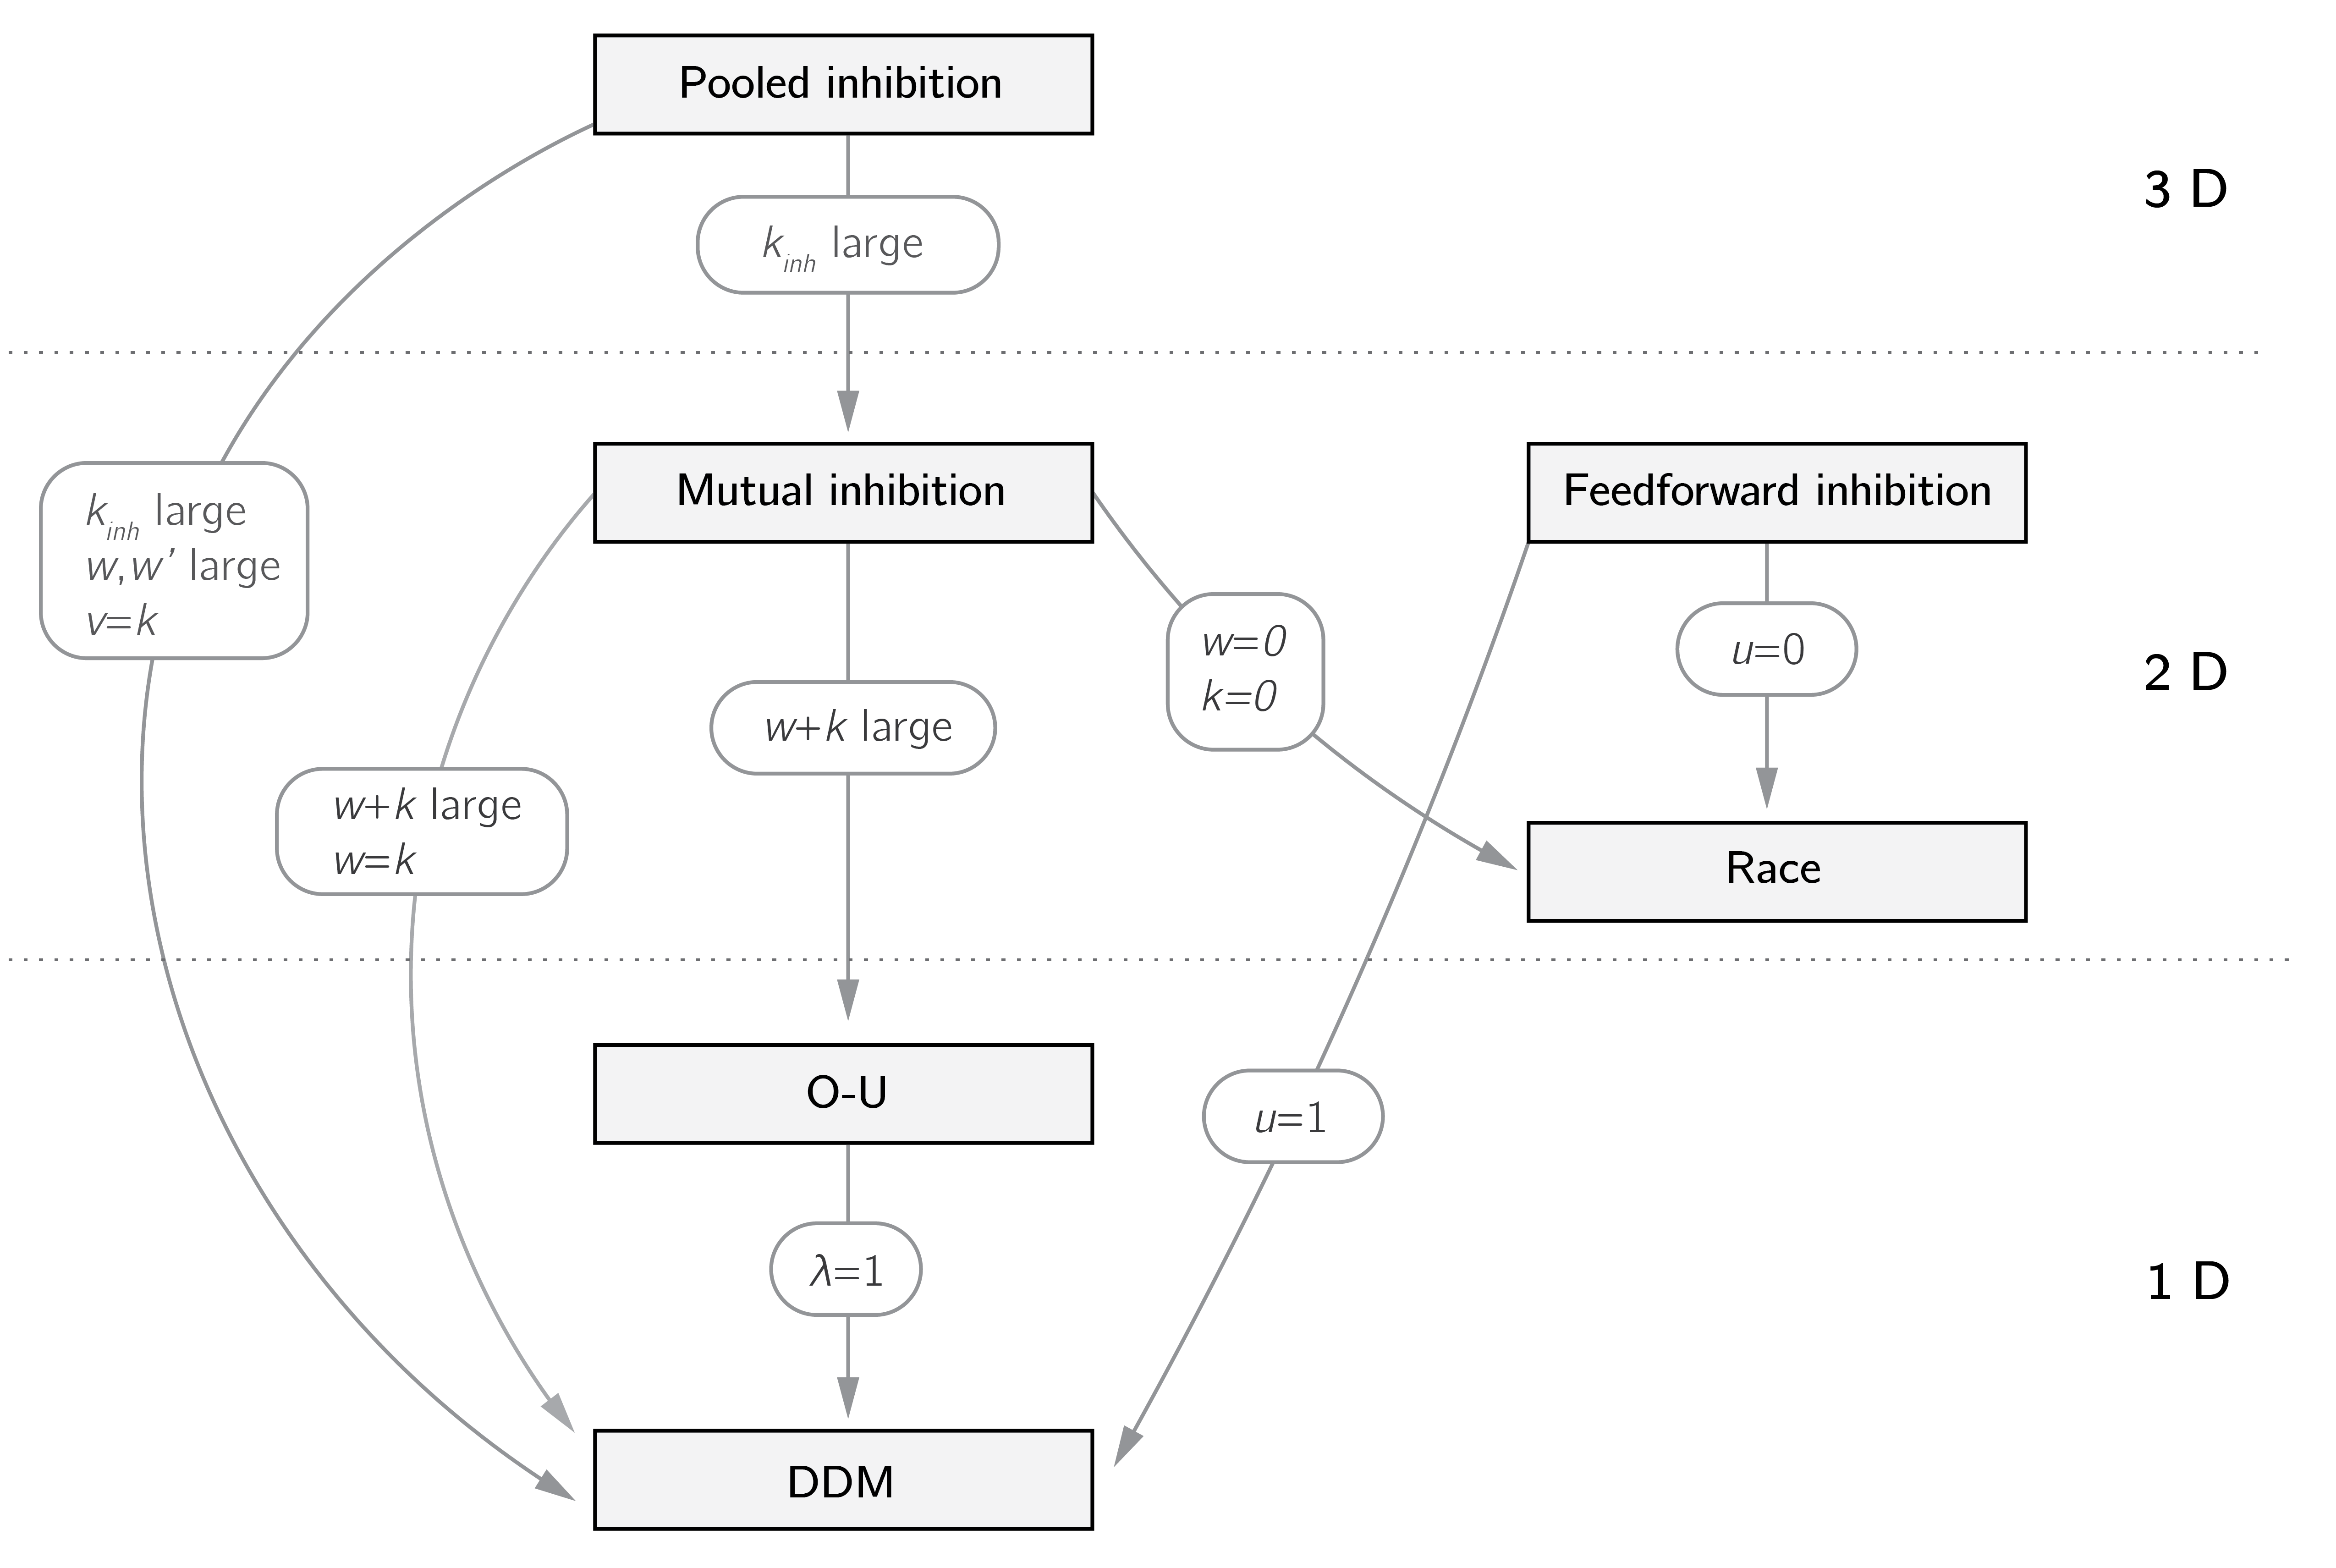
\includegraphics[width=8.33333in,height=\textheight]{media/ch4n/ch4n-8__figure57.png}

}

\caption{\label{fig-ch4n-img8-old-56}Relations between the main evidence
accumulator models of decision-making. DDM is the drift-diffusion model
which can be derived from the mutual inhibition model by setting
\(w = k\) and \(w + k\) to a large value. (Adapted from Bogacz et al.
2006).}

\end{figure}%

\subsection{Dyadic models}\label{sec-Dyadic-models}

The study of dyadic interaction lends itself to dynamic modeling. Dyadic
interactions have been studied extensively in the field of
caregiver-child interactions (Ainsworth et al. 2015). Here, we focus on
a dyadic interaction in romantic relationships.

\subsubsection{Romeo and Juliet}\label{sec-Romeo-and-Juliet}

One type of model can be traced back to publications by Rapoport (1960)
and Strogatz (1988). I follow the setup described by Sprott (2004). Note
that it was intended as a toy model to demonstrate dynamical modeling.

The model is about the interactions between Romeo and Juliet, where
\(R\) and \(J\) represent the feelings of Romeo and Juliet. The change
in feelings is supposed to be a function of the feelings of both people:

\begin{equation}\phantomsection\label{eq-ch4n-10-old-30}{\begin{gathered}
\frac{dR}{dt} = aR + bJ \\
\frac{dJ}{dt} = cR + dJ
\end{gathered}
}\end{equation}

First note that the case of \(b = c = 0\) resembles the exponential
model with solutions \(R = {R_{0}e}^{at}\) and \(J = {J_{0}e}^{dt}\),
which converge (to 0) or diverge (to infinity) depending on whether
\(a\) and \(d\) are negative or positive.
{\marginnote{\begin{footnotesize}Divergence in this model, unbounded
exponential growth of positive feelings, is an attractive concept but
unrealistic, I'm afraid.\end{footnotesize}}} We will see a more sensible
setup in the next model. Nevertheless, this system of coupled linear
differential equations is surprisingly rich in behavior. With the signs
of the parameters we define very different romantic styles. Strogatz
(1988) distinguishes the following:

\begin{itemize}
\item
  Eager beaver: \(a\  > \ 0,\ b\  > \ 0\), Romeo is encouraged by his
  own feelings as well as Juliet's.
\item
  Narcissistic nerd: \(a\  > \ 0,\ b\  < \ 0,\) Romeo wants more of what
  he feels but retreats from Juliet's feelings.
\item
  Cautious (secure) lover: \(a\  < \ 0,\ b\  > \ 0\), Romeo retreats
  from his own feelings but is encouraged by Juliet's.
\item
  Hermit: \(a\  < \ 0,\ b\  < \ 0,\) Romeo retreats from his own
  feelings as well as Juliet's.
\end{itemize}

Juliet may have her own style, which leads to complicated interactions.
Sprott (2004) and other sources give an extended analytical treatment of
this model. {\marginnote{\begin{footnotesize}Systems of linear
differential equations can be solved analytically, and the behavior of
the equilibria can be characterized by the eigenvalues. Some knowledge
of matrix algebra is required to understand this.\end{footnotesize}}} If
you want to learn more about dynamical systems, you should study matrix
algebra and its applications in linear dynamical systems. I have chosen
to leave it out of this book because most psychological dynamical
systems models are nonlinear. Here we just use Grind to test some cases.
I give three examples with three different sets of parameter values. In
the first case, the initial mutual interest fades; in the second case,
the relationship fizzles out after some ups and downs; and in the third
case, the couple ends up in a cycle of hate and love.

\begin{Shaded}
\begin{Highlighting}[]
\NormalTok{model }\OtherTok{\textless{}{-}} \ControlFlowTok{function}\NormalTok{(t, state, parms) \{}
  \FunctionTok{with}\NormalTok{(}\FunctionTok{as.list}\NormalTok{(}\FunctionTok{c}\NormalTok{(state,parms)), \{}
\NormalTok{    dR }\OtherTok{\textless{}{-}}\NormalTok{ a}\SpecialCharTok{*}\NormalTok{R}\SpecialCharTok{+}\NormalTok{b}\SpecialCharTok{*}\NormalTok{J}
\NormalTok{    dJ }\OtherTok{\textless{}{-}}\NormalTok{ c}\SpecialCharTok{*}\NormalTok{R}\SpecialCharTok{+}\NormalTok{d}\SpecialCharTok{*}\NormalTok{J}
    \FunctionTok{return}\NormalTok{(}\FunctionTok{list}\NormalTok{(}\FunctionTok{c}\NormalTok{(dR, dJ)))}
\NormalTok{  \})}
\NormalTok{\}}
\FunctionTok{layout}\NormalTok{(}\FunctionTok{matrix}\NormalTok{(}\DecValTok{1}\SpecialCharTok{:}\DecValTok{6}\NormalTok{,}\DecValTok{3}\NormalTok{,}\DecValTok{2}\NormalTok{,}\AttributeTok{byrow=}\NormalTok{T))}
\NormalTok{p }\OtherTok{\textless{}{-}} \FunctionTok{c}\NormalTok{(}\AttributeTok{a=}\SpecialCharTok{{-}}\DecValTok{1}\NormalTok{,}\AttributeTok{b=}\DecValTok{1}\NormalTok{,}\AttributeTok{c=}\NormalTok{.}\DecValTok{5}\NormalTok{,}\AttributeTok{d=}\SpecialCharTok{{-}}\DecValTok{1}\NormalTok{) }\CommentTok{\# parameters}
\NormalTok{s }\OtherTok{\textless{}{-}} \FunctionTok{c}\NormalTok{(}\AttributeTok{R=}\FloatTok{0.1}\NormalTok{,}\AttributeTok{J=}\NormalTok{.}\DecValTok{1}\NormalTok{) }
\FunctionTok{run}\NormalTok{()}
\FunctionTok{plane}\NormalTok{(}\AttributeTok{portrait=}\NormalTok{T,}\AttributeTok{ymin=}\SpecialCharTok{{-}}\DecValTok{1}\NormalTok{,}\AttributeTok{xmin=}\SpecialCharTok{{-}}\DecValTok{1}\NormalTok{,}\AttributeTok{grid=}\DecValTok{3}\NormalTok{,}\AttributeTok{vector=}\NormalTok{T,}\AttributeTok{legend=}\NormalTok{F)}
\NormalTok{p }\OtherTok{\textless{}{-}} \FunctionTok{c}\NormalTok{(}\AttributeTok{a=}\SpecialCharTok{{-}}\NormalTok{.}\DecValTok{2}\NormalTok{,}\AttributeTok{b=}\SpecialCharTok{{-}}\DecValTok{1}\NormalTok{,}\AttributeTok{c=}\DecValTok{1}\NormalTok{,}\AttributeTok{d=}\DecValTok{0}\NormalTok{) }\CommentTok{\# parameters}
\FunctionTok{run}\NormalTok{(}\AttributeTok{ymin=}\SpecialCharTok{{-}}\NormalTok{.}\DecValTok{2}\NormalTok{,}\AttributeTok{legend=}\NormalTok{F)}
\FunctionTok{plane}\NormalTok{(}\AttributeTok{portrait=}\NormalTok{T,}\AttributeTok{ymin=}\SpecialCharTok{{-}}\DecValTok{1}\NormalTok{,}\AttributeTok{xmin=}\SpecialCharTok{{-}}\DecValTok{1}\NormalTok{,}\AttributeTok{grid=}\DecValTok{2}\NormalTok{,}\AttributeTok{tstep=}\NormalTok{.}\DecValTok{001}\NormalTok{,}\AttributeTok{legend=}\NormalTok{F)}
\NormalTok{p }\OtherTok{\textless{}{-}} \FunctionTok{c}\NormalTok{(}\AttributeTok{a=}\SpecialCharTok{{-}}\NormalTok{.}\DecValTok{1}\NormalTok{,}\AttributeTok{b=}\SpecialCharTok{{-}}\DecValTok{1}\NormalTok{,}\AttributeTok{c=}\DecValTok{1}\NormalTok{,}\AttributeTok{d=}\FloatTok{0.1}\NormalTok{) }\CommentTok{\# parameters}
\FunctionTok{run}\NormalTok{(}\AttributeTok{ymin=}\SpecialCharTok{{-}}\NormalTok{.}\DecValTok{2}\NormalTok{,}\AttributeTok{legend=}\NormalTok{F)}
\FunctionTok{plane}\NormalTok{(}\AttributeTok{portrait=}\NormalTok{T,}\AttributeTok{ymin=}\SpecialCharTok{{-}}\DecValTok{1}\NormalTok{,}\AttributeTok{xmin=}\SpecialCharTok{{-}}\DecValTok{1}\NormalTok{,}\AttributeTok{grid=}\DecValTok{3}\NormalTok{,}\AttributeTok{tstep=}\NormalTok{.}\DecValTok{001}\NormalTok{,}\AttributeTok{legend=}\NormalTok{F)}
\end{Highlighting}
\end{Shaded}

\begin{figure}

\centering{

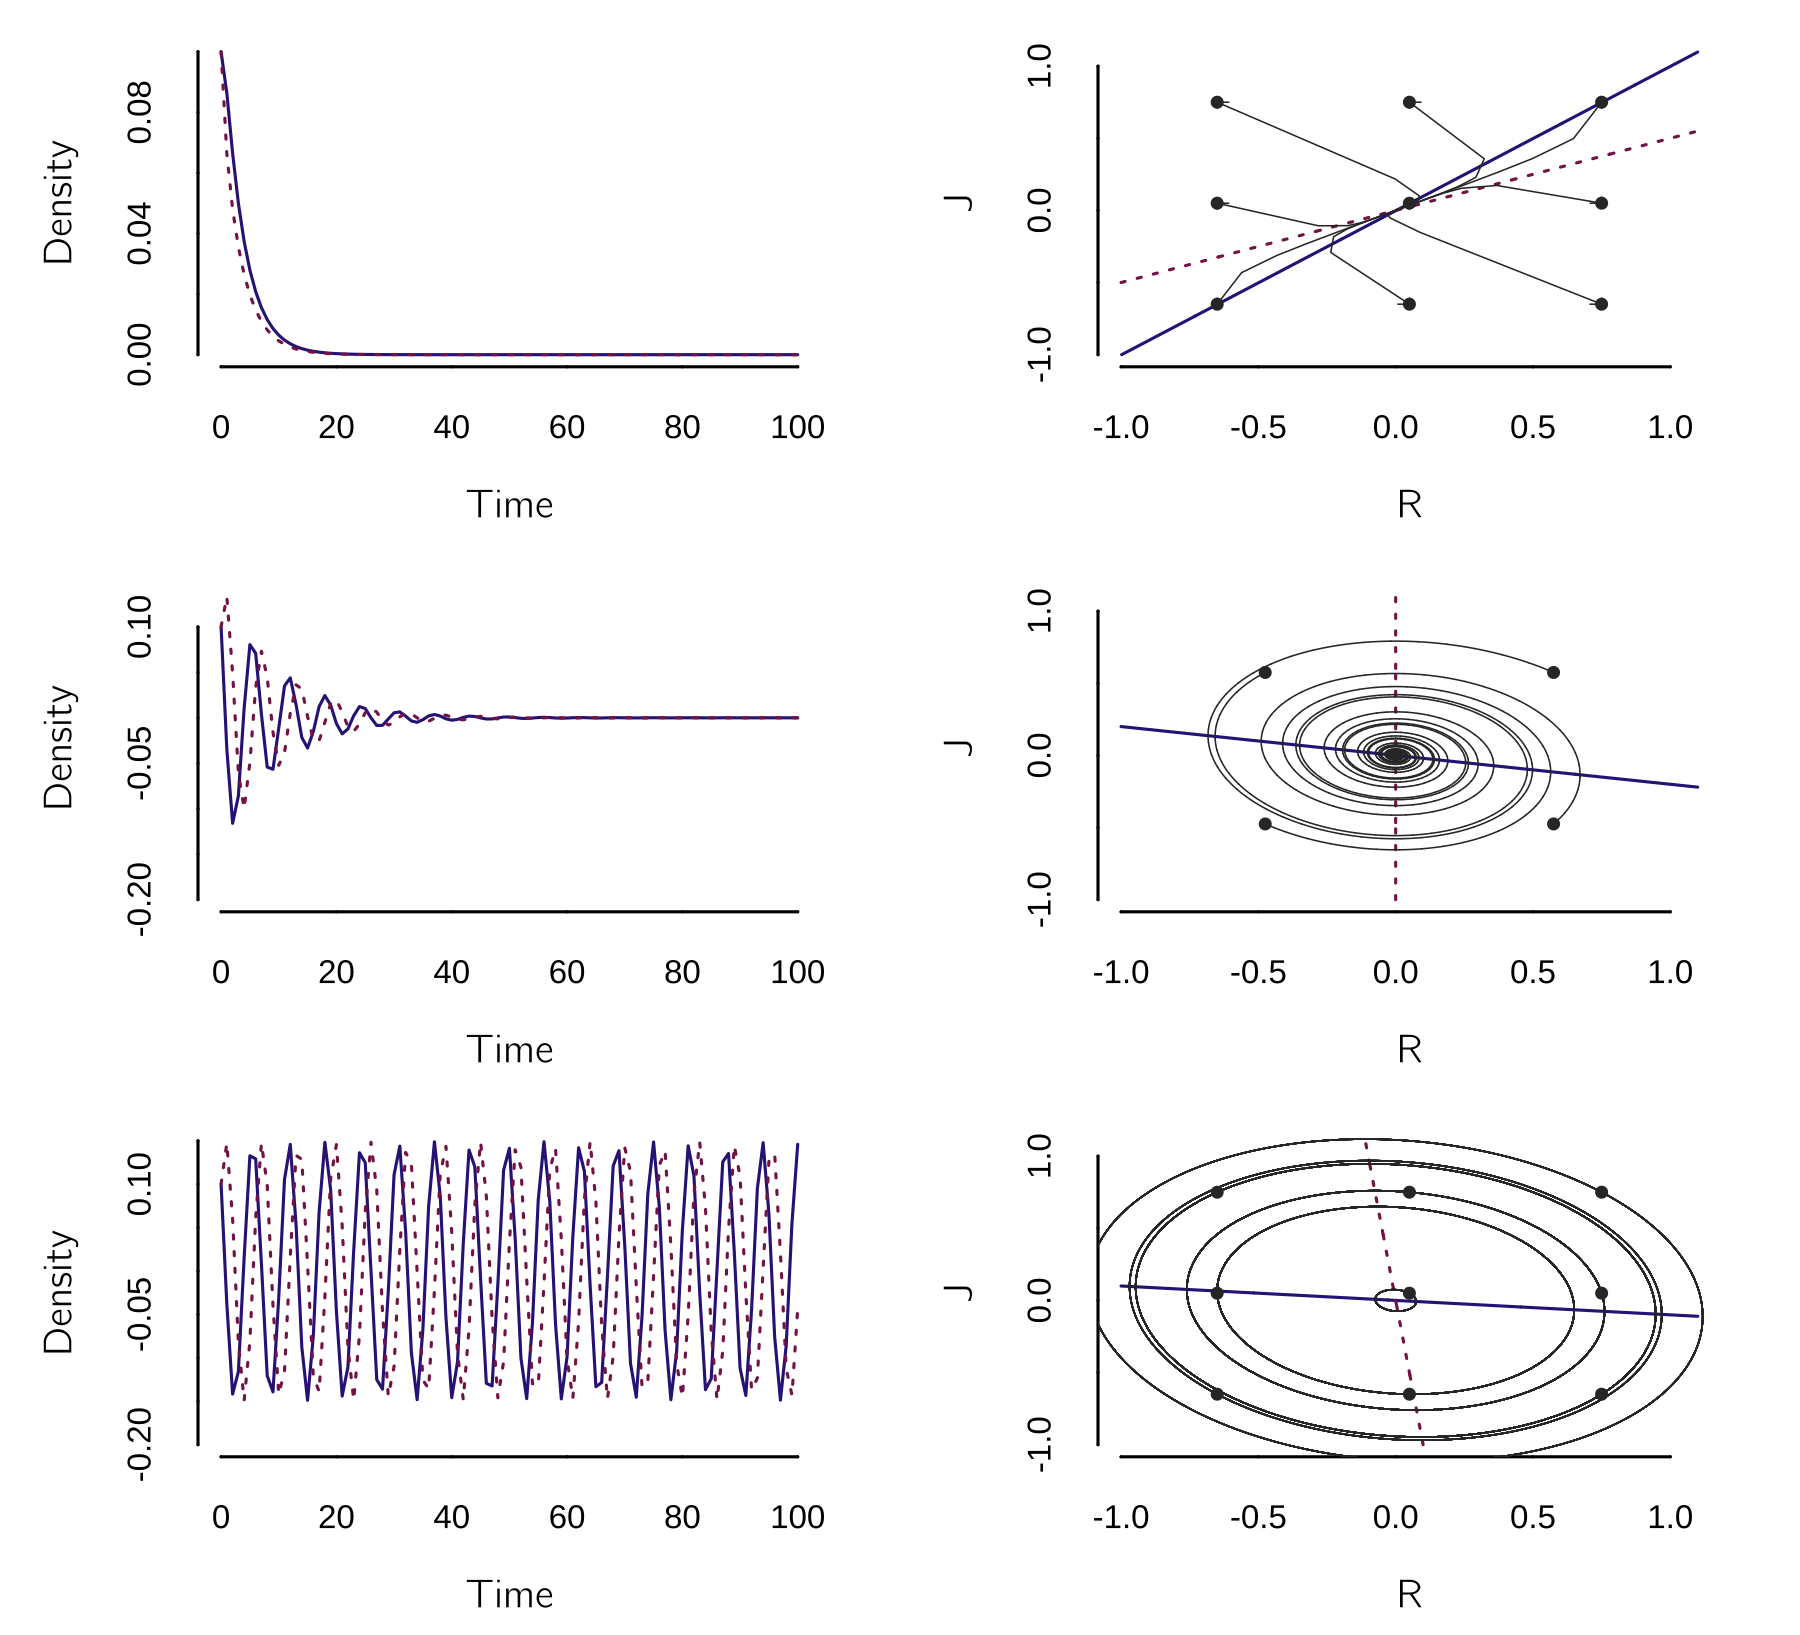
\includegraphics[width=9.375in,height=\textheight]{media/ch4n/fig-ch4n-img9-old-57.png}

}

\caption{\label{fig-ch4n-img9-old-57}Three different love affairs
between Romeo and Juliet.}

\end{figure}%

The lines in the phase plots in figure~\ref{fig-ch4n-img9-old-57} are
the nullclines. {\marginnote{\begin{footnotesize}Nullclines are the
curves for which the time derivatives of the behavioral variables \(R\)
and \(J\) are 0.\end{footnotesize}}} In linear dynamical system,
nullclines are straight lines. Where they intersect, stable or unstable
fixed points can occur. Depending on the angle between the nullclines,
we get a fixed point (first two cases), a limit cycle (last case), or
divergence (not shown).

Rinaldi (1998) proposed an extension and a constraint to the model that
makes it a bit more realistic and easier to study. The basic equation is
now \(dR/dt = - aR + bJ + A_{J}\), where \(a\) is interpreted as a
forgetting parameter (constrained to be positive) and \(A_{J}\) is the
attractiveness of the Juliet. In this case, a necessary and sufficient
condition for asymptotic stability (i.e., having a fixed point) is that
\(ad > bc\).

Rinaldi also considers the case of a population of heterosexual men and
women with different levels of attractiveness. The idea is that a man
and a woman will leave their current partners and bond together when
both reach a more optimal level of love. Rinaldi analyzes the conditions
under which the population reaches a stable state. This marriage
assignment problem, as it is called, is an example of a famous problem
in optimization theory known as an assignment problem. The goal is to
find a stable assignment of men to women, such that no man and woman
prefer each other to their current partners (Gale and Shapley 1962). We
use such algorithms to assign students to master tracks in our
educational program.

Some other advanced variations of this model have been proposed. In
these papers the analysis of the mathematical properties of the model
gets much more attention than the psychological theory. It is often
unclear what, exactly, the variables are and what the reasoning behind
certain model assumptions . The work of Murray and Gottman, discussed in
the next section, is more interesting in this regard.

\subsubsection{The mathematics of
marriage}\label{sec-The-mathematics-of-marriage}

The model of marriage developed by the psychologist John Gottman and the
mathematical biologist James Murray (2002) is firmly grounded in
psychological theory and data. The main phenomenon that inspired this
modeling work is Gottman and Levenson's (1992) finding that the patterns
of interaction between couples, when discussing a major area of ongoing
disagreement in their marriage, are predictive of divorce.

The model consists of two coupled difference equations, but I present it
in the form of differential equations.\footnote{Difference equations
  were used in the original model because the data consist of turn
  takings in a conversation. This, however, does not lead to qualitative
  different results. With
  \texttt{method=\textquotesingle{}euler\textquotesingle{}} and a change
  in \(r_{w}\) and \(r_{h}\) the difference model can be constructed.}

\begin{equation}\phantomsection\label{eq-ch4n-11-old-31}{
\begin{gathered}
\frac{dW}{dt} = I_{w}(H,a,b) - r_{w}W + W_{e}, \\
\frac{dH}{dt} = I_{h}(W,a,b) - r_{h}H + H_{e},
\end{gathered}
}\end{equation}

where the influence functions \(I_{w}\) and \(I_{h}\) are defined as:

\begin{equation}\phantomsection\label{eq-ch4n-12-old-32}{
I(x,a,b) = \frac{sign(x)}{1 + e^{a\left( |x| - b \right)}}.
}\end{equation}

I made up this flexible function to allow for very different forms of
influence (as we will see below). When both influences are 0
(\(a = - 8,b = - \infty\)), the state or mood of the wife (\(W\)) and
the husband (\(H\)) converge to \(W_{e}\) and \(H_{e}\), with rates
\(r_{w}\) and \(r_{h}\), respectively. \(W_{e}\) and \(H_{e}\) are the
uninfluenced steady states of mood when the spouses do not
interact.\footnote{I follow the definition and notation of the original
  source, but this model is clearly not restricted to heterosexual
  relationships.}

However, if the influence function (\(a = - 8, b = 0\)) is such that a
positive mood in one spouse provokes a positive mood in the other, while
a negative mood provokes a negative mood, we expect a negative and a
positive equilibrium depending on the initial states and uninfluenced
steady state values.

Another more complex influence function (\(a = - 8, b = 1\)) assumes
that only extreme mood states influence the other spouse.

This is implemented with:

\begin{Shaded}
\begin{Highlighting}[]
\NormalTok{model }\OtherTok{\textless{}{-}} \ControlFlowTok{function}\NormalTok{(t, state, parms) \{}
  \FunctionTok{with}\NormalTok{(}\FunctionTok{as.list}\NormalTok{(}\FunctionTok{c}\NormalTok{(state,parms)), \{}
\NormalTok{    dW }\OtherTok{\textless{}{-}} \FunctionTok{influence}\NormalTok{(H,a,b)}\SpecialCharTok{{-}}\NormalTok{rw}\SpecialCharTok{*}\NormalTok{W}\SpecialCharTok{+}\NormalTok{We}
\NormalTok{    dH }\OtherTok{\textless{}{-}} \FunctionTok{influence}\NormalTok{(W,a,b)}\SpecialCharTok{{-}}\NormalTok{rh}\SpecialCharTok{*}\NormalTok{H}\SpecialCharTok{+}\NormalTok{He}
    \FunctionTok{return}\NormalTok{(}\FunctionTok{list}\NormalTok{(}\FunctionTok{c}\NormalTok{(dW,dH)))}
\NormalTok{  \})}
\NormalTok{\}}
\FunctionTok{layout}\NormalTok{(}\FunctionTok{matrix}\NormalTok{(}\DecValTok{1}\SpecialCharTok{:}\DecValTok{9}\NormalTok{,}\DecValTok{3}\NormalTok{,}\DecValTok{3}\NormalTok{,}\AttributeTok{byrow=}\NormalTok{T))}
\FunctionTok{par}\NormalTok{(}\AttributeTok{mar=}\FunctionTok{c}\NormalTok{(}\DecValTok{4}\NormalTok{,}\DecValTok{4}\NormalTok{,}\DecValTok{1}\NormalTok{,}\DecValTok{2}\NormalTok{))}
\NormalTok{influence }\OtherTok{\textless{}{-}} \ControlFlowTok{function}\NormalTok{(x,}\AttributeTok{a=}\SpecialCharTok{{-}}\DecValTok{8}\NormalTok{,}\AttributeTok{b=}\DecValTok{1}\NormalTok{) }\FunctionTok{sign}\NormalTok{(x)}\SpecialCharTok{/}\NormalTok{(}\DecValTok{1}\SpecialCharTok{+}\FunctionTok{exp}\NormalTok{(a}\SpecialCharTok{*}\NormalTok{(}\FunctionTok{abs}\NormalTok{(x)}\SpecialCharTok{{-}}\NormalTok{b)))}
\NormalTok{p }\OtherTok{\textless{}{-}} \FunctionTok{c}\NormalTok{(}\AttributeTok{rw=}\NormalTok{.}\DecValTok{6}\NormalTok{,}\AttributeTok{rh=}\NormalTok{.}\DecValTok{6}\NormalTok{,}\AttributeTok{We=}\NormalTok{.}\DecValTok{18}\NormalTok{,}\AttributeTok{He=}\SpecialCharTok{{-}}\NormalTok{.}\DecValTok{18}\NormalTok{,}\AttributeTok{a=}\SpecialCharTok{{-}}\DecValTok{8}\NormalTok{,}\AttributeTok{b=}\ConstantTok{Inf}\NormalTok{)}
\NormalTok{s }\OtherTok{\textless{}{-}} \FunctionTok{c}\NormalTok{(}\AttributeTok{W=}\DecValTok{0}\NormalTok{,}\AttributeTok{H=}\DecValTok{0}\NormalTok{)}
\ControlFlowTok{for}\NormalTok{(b }\ControlFlowTok{in} \FunctionTok{c}\NormalTok{(}\ConstantTok{Inf}\NormalTok{,}\DecValTok{0}\NormalTok{,}\DecValTok{1}\NormalTok{))\{}
\NormalTok{p[}\StringTok{\textquotesingle{}b\textquotesingle{}}\NormalTok{] }\OtherTok{\textless{}{-}}\NormalTok{ b}
\FunctionTok{curve}\NormalTok{(}\FunctionTok{influence}\NormalTok{(x,}\SpecialCharTok{{-}}\DecValTok{8}\NormalTok{,b),}\SpecialCharTok{{-}}\DecValTok{3}\NormalTok{,}\DecValTok{3}\NormalTok{,}\AttributeTok{xlab=}\StringTok{\textquotesingle{}W\textquotesingle{}}\NormalTok{,}\AttributeTok{ylab=}\StringTok{\textquotesingle{}H\textquotesingle{}}\NormalTok{,}\AttributeTok{lwd=}\DecValTok{2}\NormalTok{)}
\FunctionTok{plane}\NormalTok{(}\AttributeTok{xmin=}\SpecialCharTok{{-}}\FloatTok{2.5}\NormalTok{,}\AttributeTok{xmax=}\FloatTok{2.5}\NormalTok{,}\AttributeTok{ymin=}\SpecialCharTok{{-}}\DecValTok{2}\NormalTok{,}\AttributeTok{ymax=}\DecValTok{2}\NormalTok{,}\AttributeTok{legend=}\NormalTok{F)}
\ControlFlowTok{for}\NormalTok{(i }\ControlFlowTok{in} \FunctionTok{seq}\NormalTok{(}\SpecialCharTok{{-}}\DecValTok{2}\NormalTok{,}\DecValTok{2}\NormalTok{,}\AttributeTok{by=}\NormalTok{.}\DecValTok{25}\NormalTok{)) }\FunctionTok{newton}\NormalTok{(}\AttributeTok{s=}\FunctionTok{c}\NormalTok{(}\AttributeTok{W=}\NormalTok{i,}\AttributeTok{H=}\NormalTok{i),}\AttributeTok{plot=}\NormalTok{T)}
\ControlFlowTok{for}\NormalTok{ (i }\ControlFlowTok{in} \DecValTok{1}\SpecialCharTok{:}\DecValTok{100}\NormalTok{)}
  \FunctionTok{run}\NormalTok{(}\AttributeTok{state=}\FunctionTok{c}\NormalTok{(}\AttributeTok{W=}\FunctionTok{rnorm}\NormalTok{(}\DecValTok{1}\NormalTok{,}\DecValTok{0}\NormalTok{,.}\DecValTok{5}\NormalTok{),}\AttributeTok{H=}\FunctionTok{rnorm}\NormalTok{(}\DecValTok{1}\NormalTok{,}\DecValTok{0}\NormalTok{,}\DecValTok{1}\NormalTok{)), }\AttributeTok{tmax=}\DecValTok{50}\NormalTok{,}\AttributeTok{ymin=}\SpecialCharTok{{-}}\DecValTok{2}\NormalTok{,}
      \AttributeTok{ymax=}\DecValTok{2}\NormalTok{,}\AttributeTok{add=}\NormalTok{(i}\SpecialCharTok{\textgreater{}}\DecValTok{1}\NormalTok{),}\AttributeTok{legend=}\NormalTok{F)}
\NormalTok{\}}
\end{Highlighting}
\end{Shaded}

This results in figure~\ref{fig-ch4n-img10-old-58}.

\begin{figure}

\centering{

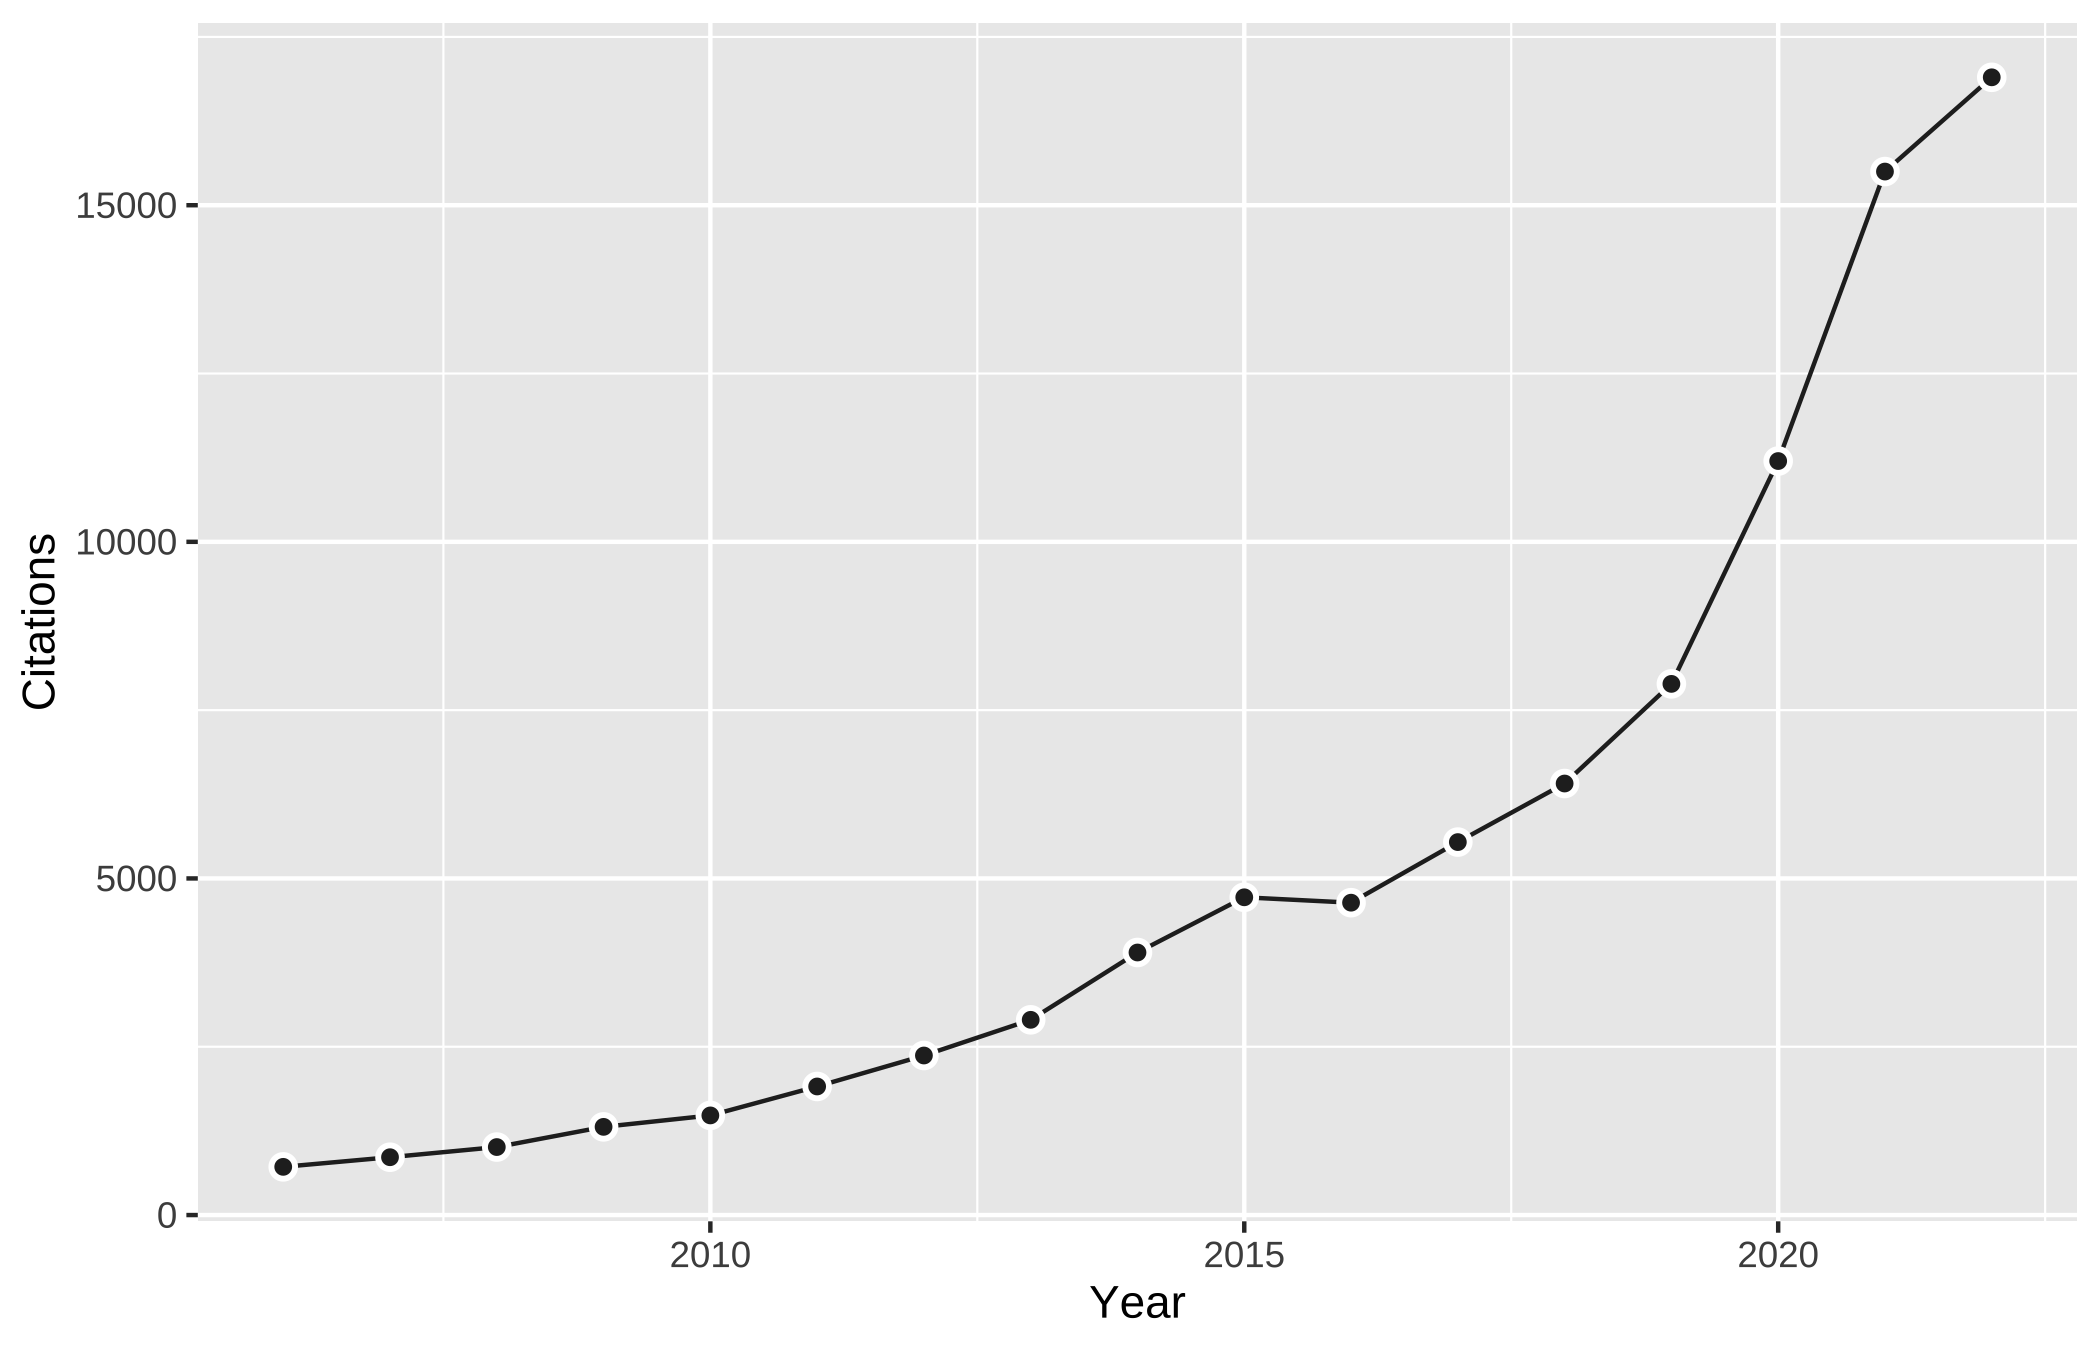
\includegraphics[width=9.375in,height=\textheight]{media/ch4n/fig-ch4n-img10-old-58.png}

}

\caption{\label{fig-ch4n-img10-old-58}Qualitative difference marriage
equilibrium landscapes depending on the form of the influence function.
In the first (top), they simply have no influence and both partners
converge to their uninfluenced steady states of mood. In the second
(middle) , the response to the partner's mood is extreme, resulting in
either a positive or negative mutual state. In the last case (bottom),
the response to low positive or negative moods is close to 0 but extreme
at higher levels. Now there are three stable states.}

\end{figure}%

The three influence functions are shown in the first column, the
nullclines in the second, and a series of runs from random initial
states in the third. The first case shows that the moods converge to
\(W_{e}\) and \(H_{e}\), when there is no mutual influence. The second
has two equilibria, with an unstable fixed point in the middle, while
the last case has five fixed points, three of which are stable.

I have kept the influence functions and most parameters the same for
both spouses, but this is not necessarily the case. It is possible to
derive the equilibria analytically and to determine the stability of
these equilibria (Gottman et al. 2002). They also propose a two-stage
procedure for fitting the model to data consisting of positive and
negative speaker interactions using a bilinear influence function. A
more advanced statistical approach is proposed in Ellen L. Hamaker,
Zhang, and van~der Maas (2009). For a related model for the interaction
between therapist and client, see Tschacher and Haken (2019).

\subsection{The van Geert models}\label{sec-The-van-Geert-models}

In a series of papers, Paul van Geert proposed dynamical systems models
for developmental processes (Den Hartigh et al. 2016; van Geert 1998,
1991). {\marginnote{\begin{footnotesize}It is thought that cognitive and
language abilities grow over time in an autocatalytic process
constrained by a limited capacity, similar to the logistic growth of
populations.\end{footnotesize}}}

Van Geert has proposed many different models, but I will give just one
example. Van Geert (1991) introduced a system of two coupled difference
equations to model where the growth rate of one cognitive ability
depends on the level of another cognitive ability:

\begin{equation}\phantomsection\label{eq-ch4n-13-old-33}{
\begin{gathered}
X_{t + 1} = (a - bY_{t})X_{t} - \frac{aX_{t}^{2}}{K} \\
Y_{t + 1} = (c - dX_{t})Y_{t} - \frac{cY_{t}^{2}}{K}
\end{gathered}
}\end{equation}

This can be implemented as follows:

\begin{Shaded}
\begin{Highlighting}[]
\NormalTok{model }\OtherTok{\textless{}{-}} \ControlFlowTok{function}\NormalTok{(t, state, parms) \{}
  \FunctionTok{with}\NormalTok{(}\FunctionTok{as.list}\NormalTok{(}\FunctionTok{c}\NormalTok{(state,parms)), \{}
\NormalTok{    dX }\OtherTok{\textless{}{-}}\NormalTok{ (a }\SpecialCharTok{+}\NormalTok{ b }\SpecialCharTok{*}\NormalTok{ Y) }\SpecialCharTok{*}\NormalTok{ X }\SpecialCharTok{{-}}\NormalTok{ a }\SpecialCharTok{*}\NormalTok{ X}\SpecialCharTok{\^{}}\DecValTok{2} \SpecialCharTok{/}\NormalTok{ K}
\NormalTok{    dY }\OtherTok{\textless{}{-}}\NormalTok{ (c }\SpecialCharTok{+}\NormalTok{ d }\SpecialCharTok{*}\NormalTok{ X) }\SpecialCharTok{*}\NormalTok{ Y }\SpecialCharTok{{-}}\NormalTok{ c }\SpecialCharTok{*}\NormalTok{ Y}\SpecialCharTok{\^{}}\DecValTok{2} \SpecialCharTok{/}\NormalTok{ K}
    \FunctionTok{return}\NormalTok{(}\FunctionTok{list}\NormalTok{(}\FunctionTok{c}\NormalTok{(dX, dY)))}
\NormalTok{  \}) \}}

\FunctionTok{layout}\NormalTok{(}\FunctionTok{matrix}\NormalTok{(}\DecValTok{1}\SpecialCharTok{:}\DecValTok{4}\NormalTok{,}\DecValTok{2}\NormalTok{,}\DecValTok{2}\NormalTok{))}
\CommentTok{\# Set parameter values and run the model:}
\NormalTok{p }\OtherTok{\textless{}{-}} \FunctionTok{c}\NormalTok{(}\AttributeTok{K =} \DecValTok{1}\NormalTok{, }\AttributeTok{a =} \FloatTok{0.4}\NormalTok{, }\AttributeTok{b =} \SpecialCharTok{{-}}\FloatTok{0.05}\NormalTok{, }\AttributeTok{c=}\NormalTok{.}\DecValTok{4}\NormalTok{, }\AttributeTok{d =} \SpecialCharTok{{-}}\FloatTok{0.15}\NormalTok{)}
\NormalTok{s }\OtherTok{\textless{}{-}} \FunctionTok{c}\NormalTok{(}\AttributeTok{X =} \FloatTok{0.01}\NormalTok{, }\AttributeTok{Y =} \FloatTok{0.01}\NormalTok{)}
\FunctionTok{run}\NormalTok{(}\AttributeTok{method =} \StringTok{"euler"}\NormalTok{, }\AttributeTok{tstep =} \DecValTok{1}\NormalTok{)}
\FunctionTok{plane}\NormalTok{(}\AttributeTok{portrait =} \ConstantTok{TRUE}\NormalTok{,}\AttributeTok{grid=}\DecValTok{4}\NormalTok{)}
\NormalTok{p }\OtherTok{\textless{}{-}} \FunctionTok{c}\NormalTok{(}\AttributeTok{K =} \DecValTok{1}\NormalTok{, }\AttributeTok{a =} \FloatTok{0.05}\NormalTok{, }\AttributeTok{b =} \SpecialCharTok{{-}}\FloatTok{0.1}\NormalTok{,  }\AttributeTok{c =} \FloatTok{0.05}\NormalTok{, }\AttributeTok{d =} \SpecialCharTok{{-}}\FloatTok{0.09}\NormalTok{)}
\NormalTok{s }\OtherTok{\textless{}{-}} \FunctionTok{c}\NormalTok{(}\AttributeTok{X =} \FloatTok{0.0126}\NormalTok{, }\AttributeTok{Y =} \FloatTok{0.01}\NormalTok{)}
\FunctionTok{run}\NormalTok{(}\AttributeTok{tmax =} \DecValTok{1500}\NormalTok{, }\AttributeTok{method =} \StringTok{"euler"}\NormalTok{, }\AttributeTok{tstep =} \DecValTok{1}\NormalTok{)}
\FunctionTok{plane}\NormalTok{(}\AttributeTok{portrait =} \ConstantTok{TRUE}\NormalTok{,}\AttributeTok{grid=}\DecValTok{4}\NormalTok{)}
\end{Highlighting}
\end{Shaded}

\begin{figure}

\centering{

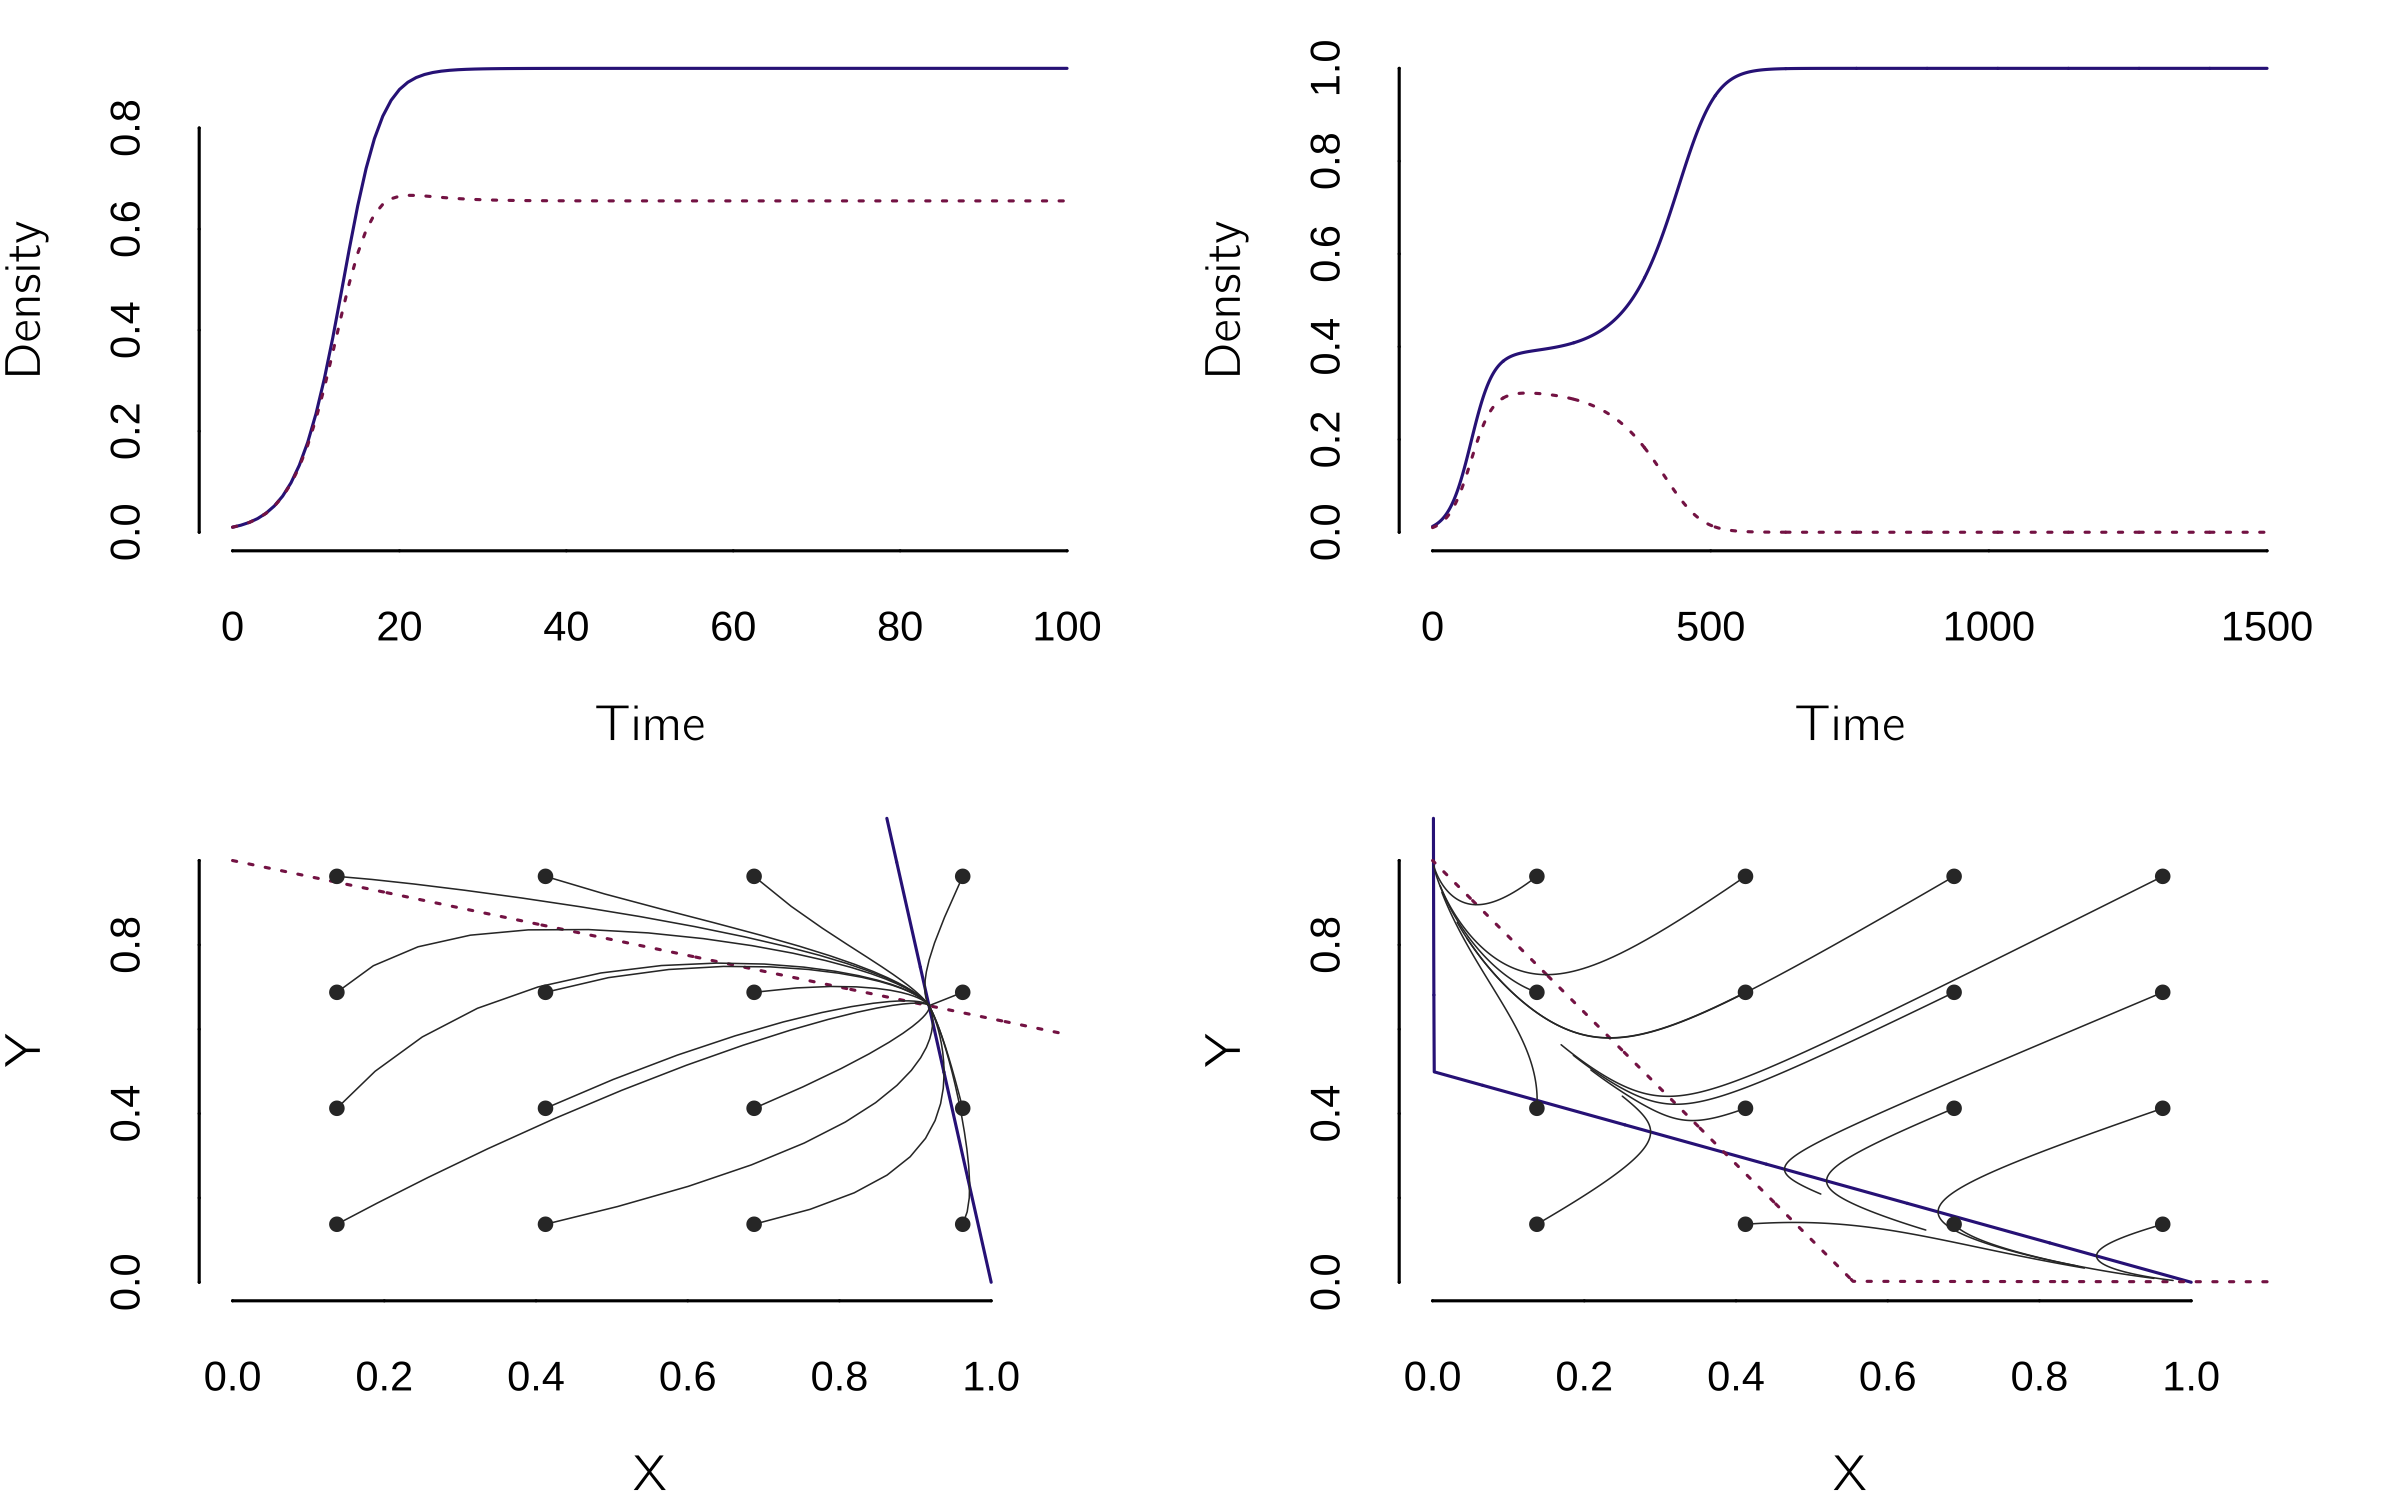
\includegraphics[width=9.375in,height=\textheight]{media/ch4n/fig-ch4n-img11-old-59.png}

}

\caption{\label{fig-ch4n-img11-old-59}The development of two
interrelated cognitive abilities in one of the van Geert models. In the
left case they coexist; in the right case one ability suppresses the
other.}

\end{figure}%

So, there are basically two outcomes: either both grow, or one grows and
suppresses the other (see figure~\ref{fig-ch4n-img11-old-59}). Note that
the method is set to ``Euler'' to simulate difference equations.

\subsection{The Pólya urn model of the third
source}\label{sec-The-Polya-Urn-model-of-the-third-source}

Another type of discrete dynamical systems model is the Pólya urn model,
which is relevant to understanding nonlinear developmental processes in
psychology. Molenaar, Boomsma, and Dolan (1993) propose the third-source
hypothesis. {\marginnote{\begin{footnotesize}The third-source hypothesis
proposes that the development of complex living systems is influenced by
three sources of variation: genetic variation, environmental variation,
and self-organizing processes.\end{footnotesize}}} Based on a series of
studies, Gärtner (1990) concluded that 70---80\% of the variation in
body weight in inbred mice appears to be due to a third component that
generates biological variability in addition to genetic and
environmental influences.

A simple, and in my opinion insightful, dynamical model for this effect
is the Pólya urn model (Mahmoud 2008). In this discrete dynamical model,
we add marbles to an urn containing some red and blue marbles. We could
start with two blue and one red marbles. We randomly take out a marble.
If it is blue, we put it back with another blue marble. If it is red, we
put it back and add a red marble. Initially, \(p(blue) = 2/3\), but what
will happen to that probability over time when we have more and more
marbles? Think about it for a moment.

My intuition was simply wrong, and in my experience, this is true for
the vast majority of people. What happens is shown in
figure~\ref{fig-ch4n-img12-old-60}. Each time you run the process,
\(p(blue)\) reaches a stable state, but the value of that state is
random. What happens is that early (random) samples have a huge
influence on the long-term dynamics. This creates a Matthew effect.
{\marginnote{\begin{footnotesize}The Matthew effect says that the rich
get richer and the poor get poorer.\end{footnotesize}}}

\begin{figure}

\centering{

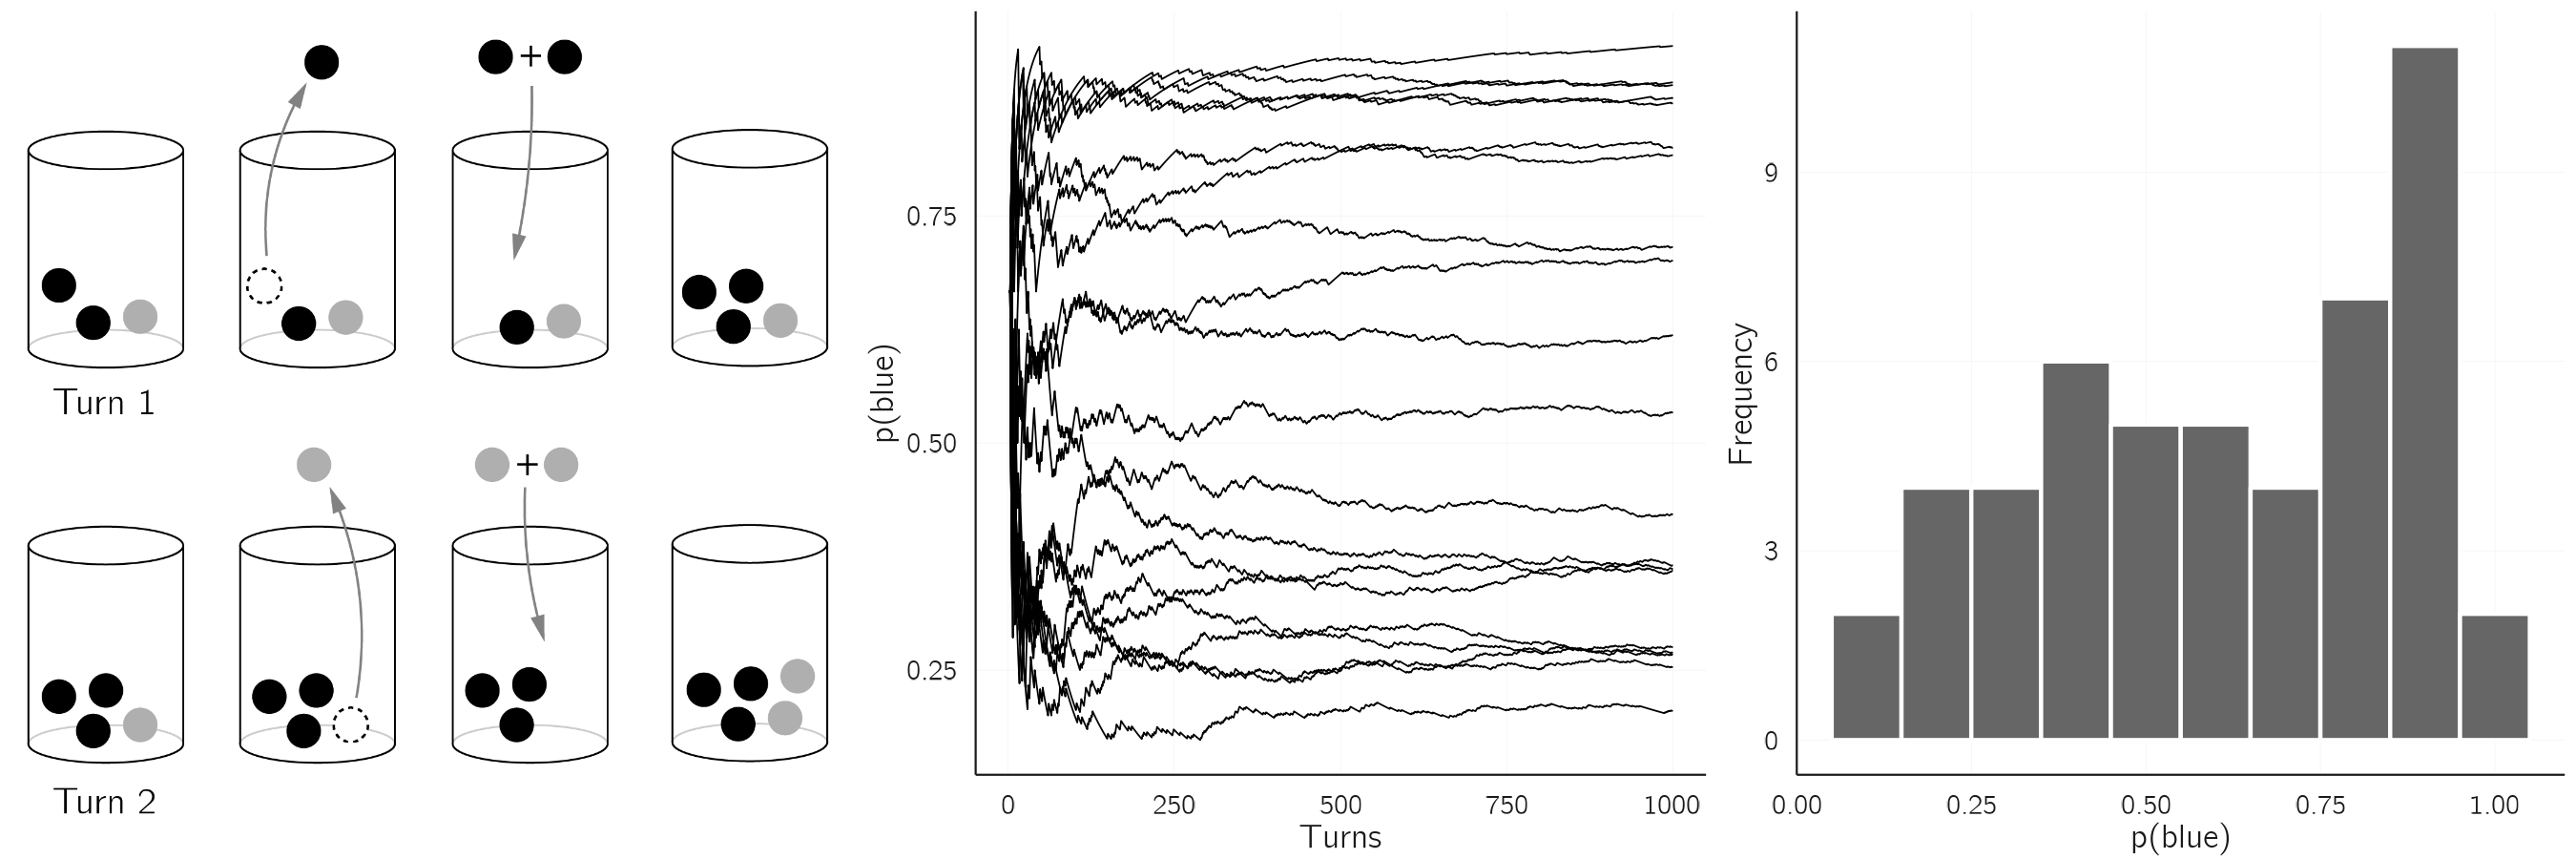
\includegraphics{media/ch4n/fig-ch4n-img12-old-60_latest.png}

}

\caption{\label{fig-ch4n-img12-old-60}The Pólya urn model. A random
marble is sampled and placed back with an extra marble of the same
color. The evolution of the probability of picking a blue marble is
unpredictable and converges to a random number. This mechanism may play
a role in the Matthew effect.}

\end{figure}%

Savi et al. (2019) provide a developmental interpretation. Imagine a
child receives a tennis racket for her birthday. First, she practices
the backhand twice at home, but incorrectly. Then, during her first
tennis lesson, her trainer demonstrates the correct backhand. She now
has three experiences, two incorrect and one correct. Now, suppose her
backhand development is based on a very simple learning schema. Whenever
a backhand return is required, she samples from her earlier experiences,
and the sampled backhand is then added to the set of earlier
experiences. Thus the cumulation of experiences follows the Pólya urn
scheme. While she has the potential to become a tennis master, her twin
sister, who had less fortunate initial experiences, decides to quit
tennis lessons within the first year. This model is consistent with many
developmental theories (e.g., the critical period hypothesis), but these
theories lack a formal approach.

\subsection{The panic model}\label{sec-The-panic-model}

In recent years, we have been working on a model of panic disorder
(Robinaugh et al. 2019). In theories of panic disorder, there is a
reinforcing feedback loop between arousal and perceived threat. When an
increase in arousal is perceived as a threat (e.g., a heart attack),
arousal increases further. This ``vicious cycle'' results in a panic
attack (D. M. Clark 1986). Thus, these theories posit two causal
effects: an effect of perceived threat on arousal and an effect of
arousal on perceived threat.

We will further assume that the effect of perceived threat on changes in
arousal is essentially linear while the causal effect of arousal on
perceived threat is nonlinear (S-shaped). For the argument, see
Robinaugh et al. (2019). It could be argued that both are nonlinear, but
this does not fundamentally change the qualitative behavior of the
model. The central part of the model consists of two coupled
differential equations:

\[\frac{dT}{dt} = - T + bA\]

\begin{equation}\phantomsection\label{eq-ch4n-14-old-34}{
\frac{dA}{dt} = \frac{1}{1 + e^{- \alpha(T + \beta)}} - A
}\end{equation}

This looks a bit like the Romeo and Juliet model, but now the effect of
perceived threat \(T\) on the change in arousal \(A\) is a logistic
function that starts at 0 and grows to 1. The location is determined by
\(\beta\), and the acceleration or steepness is determined by
\(\alpha\).

An implementation and simple illustration is:

\begin{Shaded}
\begin{Highlighting}[]
\NormalTok{model }\OtherTok{\textless{}{-}} \ControlFlowTok{function}\NormalTok{(t, state, parms) \{}
  \FunctionTok{with}\NormalTok{(}\FunctionTok{as.list}\NormalTok{(}\FunctionTok{c}\NormalTok{(state,parms)), \{}
\NormalTok{    dA }\OtherTok{\textless{}{-}} \SpecialCharTok{{-}}\NormalTok{A }\SpecialCharTok{+}\NormalTok{ b}\SpecialCharTok{*}\NormalTok{T  }
\NormalTok{    dT }\OtherTok{\textless{}{-}} \SpecialCharTok{{-}}\NormalTok{T }\SpecialCharTok{+} \DecValTok{1}\SpecialCharTok{/}\NormalTok{(}\DecValTok{1}\SpecialCharTok{+}\FunctionTok{exp}\NormalTok{(}\SpecialCharTok{{-}}\NormalTok{alpha}\SpecialCharTok{*}\NormalTok{(A}\SpecialCharTok{+}\NormalTok{beta)))}
    \FunctionTok{return}\NormalTok{(}\FunctionTok{list}\NormalTok{(}\FunctionTok{c}\NormalTok{(dA, dT)))}
\NormalTok{  \})}
\NormalTok{\}}
\NormalTok{p }\OtherTok{\textless{}{-}} \FunctionTok{c}\NormalTok{(}\AttributeTok{b=}\DecValTok{1}\NormalTok{, }\AttributeTok{alpha=}\DecValTok{12}\NormalTok{, }\AttributeTok{beta=}\SpecialCharTok{{-}}\NormalTok{.}\DecValTok{7}\NormalTok{) }
\NormalTok{s }\OtherTok{\textless{}{-}} \FunctionTok{c}\NormalTok{(}\AttributeTok{A=}\DecValTok{0}\NormalTok{, }\AttributeTok{T=}\DecValTok{0}\NormalTok{) }
\CommentTok{\# arousal increase for time t in 20:30, leads to panic, }
\CommentTok{\# which after some time (\textquotesingle{}30 min\textquotesingle{}) disappears}
\FunctionTok{layout}\NormalTok{(}\DecValTok{1}\SpecialCharTok{:}\DecValTok{2}\NormalTok{)}
\FunctionTok{plane}\NormalTok{(}\AttributeTok{vector=}\NormalTok{T,}\AttributeTok{xmin=}\DecValTok{0}\NormalTok{,}\AttributeTok{ymin=}\DecValTok{0}\NormalTok{,}\AttributeTok{xmax=}\DecValTok{1}\NormalTok{,}\AttributeTok{ymax=}\FloatTok{1.1}\NormalTok{,}\AttributeTok{legend=}\NormalTok{F) }
\FunctionTok{newton}\NormalTok{(}\AttributeTok{s=}\FunctionTok{c}\NormalTok{(}\AttributeTok{A=}\DecValTok{0}\NormalTok{,}\AttributeTok{T=}\DecValTok{0}\NormalTok{),}\AttributeTok{plot=}\NormalTok{T)}
\FunctionTok{newton}\NormalTok{(}\AttributeTok{s=}\FunctionTok{c}\NormalTok{(}\AttributeTok{A=}\FloatTok{0.8}\NormalTok{,}\AttributeTok{T=}\NormalTok{.}\DecValTok{8}\NormalTok{),}\AttributeTok{plot=}\NormalTok{T)}
\FunctionTok{newton}\NormalTok{(}\AttributeTok{s=}\FunctionTok{c}\NormalTok{(}\AttributeTok{A=}\DecValTok{1}\NormalTok{,}\AttributeTok{T=}\DecValTok{1}\NormalTok{),}\AttributeTok{plot=}\NormalTok{T);}
\FunctionTok{run}\NormalTok{(}\AttributeTok{after=}\StringTok{"if(t\textgreater{}20\&t\textless{}30)state[1]\textless{}{-}1;state\textless{}{-}state+rnorm(2,mean=0,sd=0.1)"}\NormalTok{)}
\end{Highlighting}
\end{Shaded}

The \(\beta\) parameter is set so that the nonpanic mode dominates, but
the panic mode is present (a metastable state). This state can be easily
disturbed (see plane). For \(20 < t < 30\), arousal is set to a high
value, resulting in a high perceived threat. But because we also added
some noise to both processes, after some time both arousal and perceived
threat jump back to low values.

This dynamic of this model is the cusp, as can be checked with (see
figure~\ref{fig-ch4n-img15-old-63}):

\begin{Shaded}
\begin{Highlighting}[]
\NormalTok{p }\OtherTok{\textless{}{-}} \FunctionTok{c}\NormalTok{(}\AttributeTok{b=}\DecValTok{1}\NormalTok{,}\AttributeTok{alpha=}\DecValTok{12}\NormalTok{,}\AttributeTok{beta=}\SpecialCharTok{{-}}\NormalTok{.}\DecValTok{5}\NormalTok{)}
\NormalTok{start }\OtherTok{\textless{}{-}} \FunctionTok{newton}\NormalTok{(}\AttributeTok{s=}\FunctionTok{c}\NormalTok{(}\AttributeTok{A=}\NormalTok{.}\DecValTok{1}\NormalTok{,}\AttributeTok{T=}\NormalTok{.}\DecValTok{1}\NormalTok{)) }
\FunctionTok{continue}\NormalTok{(start,}\AttributeTok{x=}\StringTok{"beta"}\NormalTok{,}\AttributeTok{y=}\StringTok{"T"}\NormalTok{,}\AttributeTok{xmin=}\SpecialCharTok{{-}}\DecValTok{1}\NormalTok{,}\AttributeTok{xmax=}\DecValTok{1}\NormalTok{,}\AttributeTok{ymax=}\DecValTok{1}\NormalTok{) }
\FunctionTok{continue}\NormalTok{(start,}\AttributeTok{x=}\StringTok{"alpha"}\NormalTok{,}\AttributeTok{y=}\StringTok{"T"}\NormalTok{,}\AttributeTok{xmin=}\SpecialCharTok{{-}}\DecValTok{1}\NormalTok{,}\AttributeTok{xmax=}\DecValTok{20}\NormalTok{,}\AttributeTok{ymax=}\DecValTok{1}\NormalTok{) }
\NormalTok{start }\OtherTok{\textless{}{-}} \FunctionTok{newton}\NormalTok{(}\AttributeTok{s=}\FunctionTok{c}\NormalTok{(}\AttributeTok{A=}\DecValTok{1}\NormalTok{,}\AttributeTok{T=}\DecValTok{1}\NormalTok{)) }\CommentTok{\# finds a minimum starting from X = {-}1}
\FunctionTok{continue}\NormalTok{(start,}\AttributeTok{x=}\StringTok{"alpha"}\NormalTok{,}\AttributeTok{y=}\StringTok{"T"}\NormalTok{,}\AttributeTok{xmin=}\SpecialCharTok{{-}}\DecValTok{1}\NormalTok{,}\AttributeTok{xmax=}\DecValTok{20}\NormalTok{,}\AttributeTok{ymax=}\DecValTok{1}\NormalTok{,}\AttributeTok{add=}\NormalTok{T) }
\end{Highlighting}
\end{Shaded}

In Robinaugh et al. (2019), this model is extended with other processes,
such as arousal and escape schemes, that operate on the parameters of
the basic model. These are slower processes that are modeled on
different time scales.

\begin{figure}

\centering{

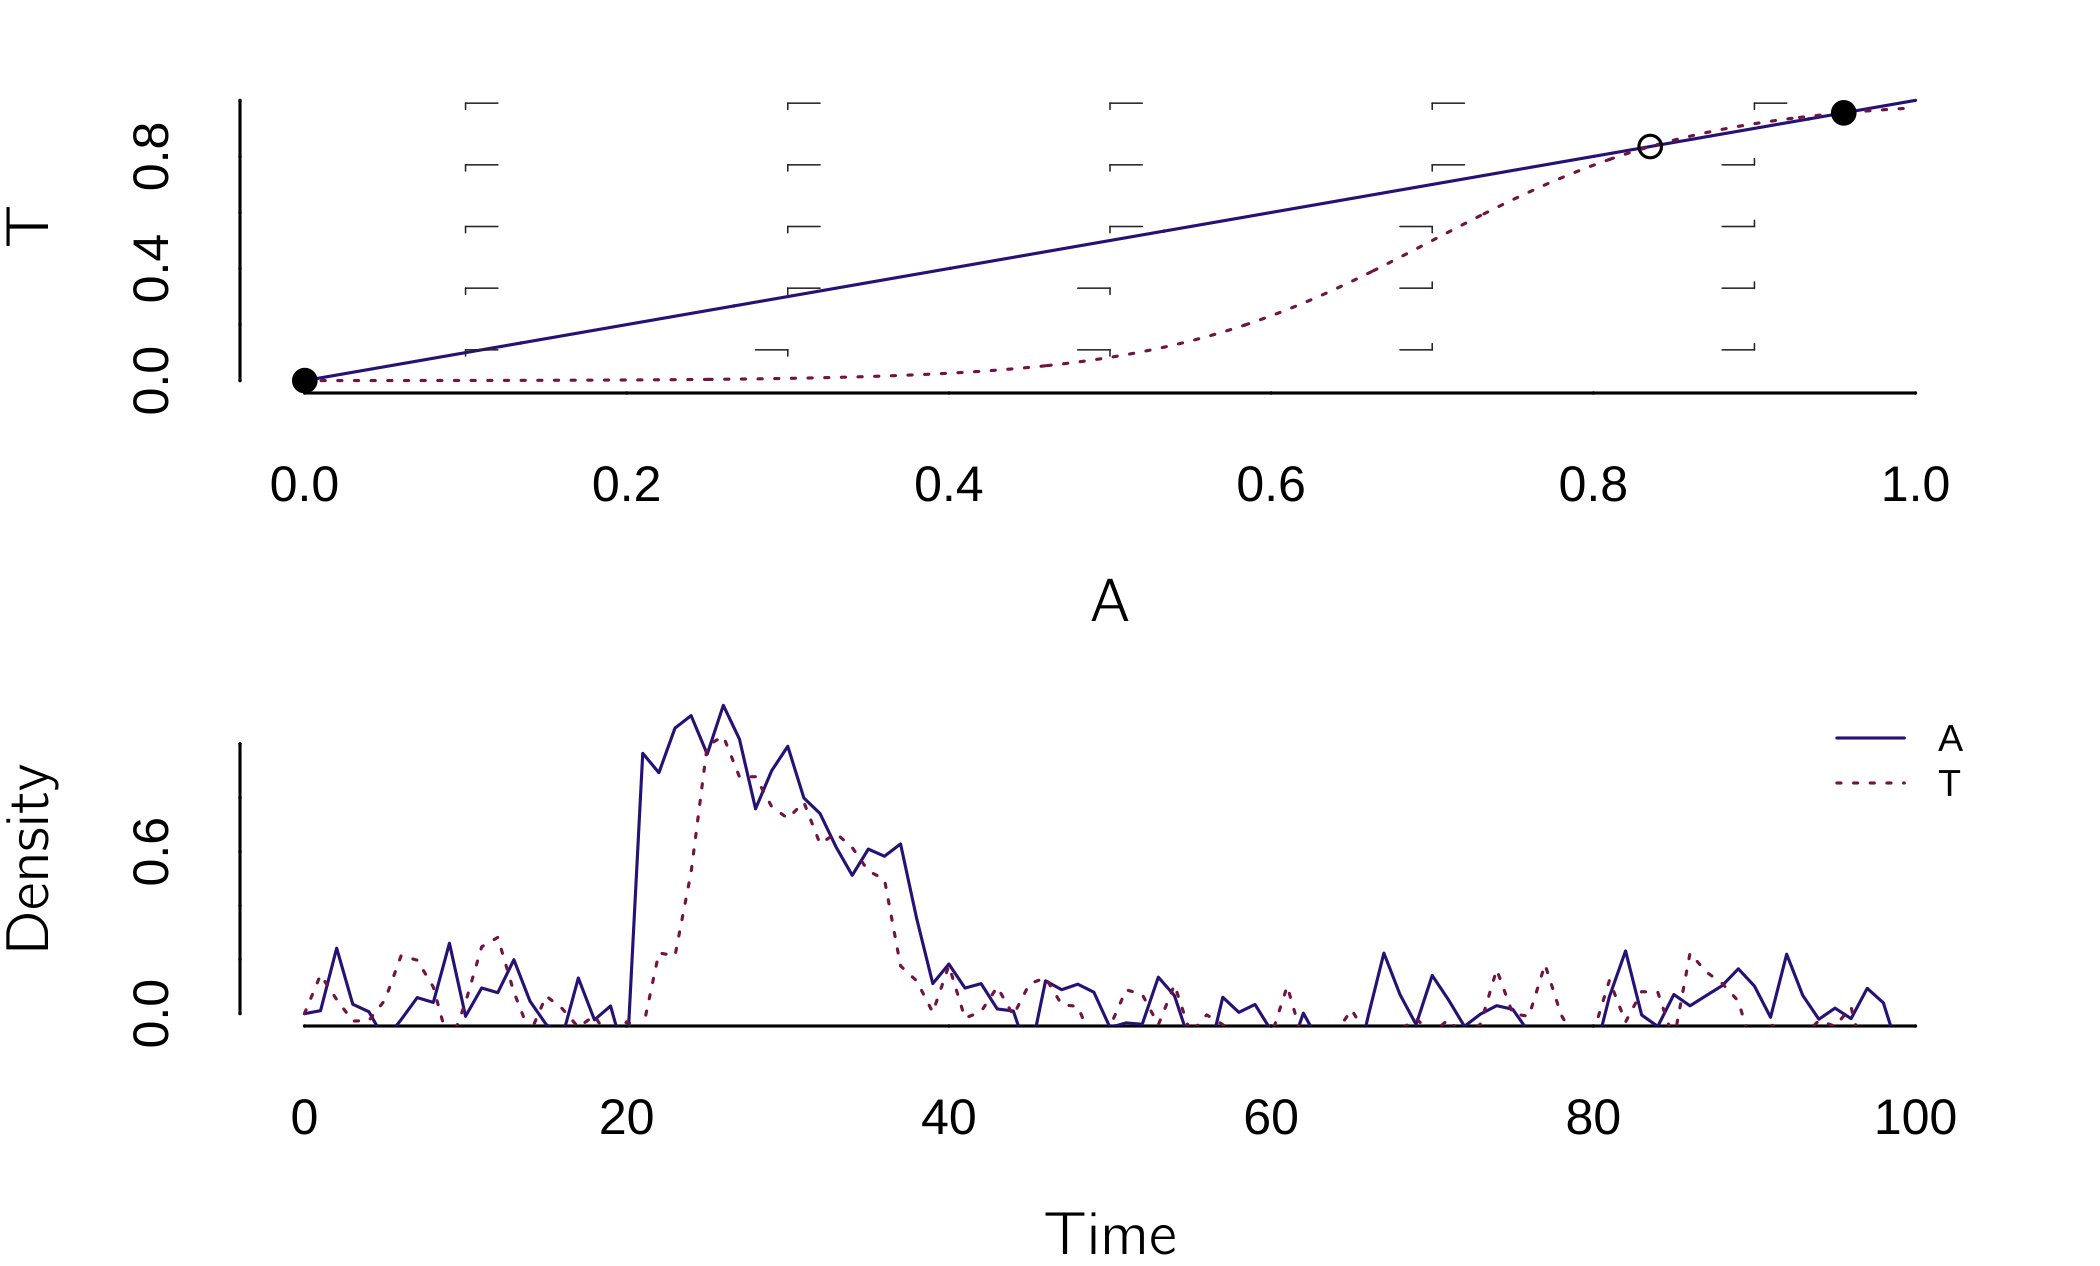
\includegraphics[width=8.33333in,height=\textheight]{media/ch4n/fig-ch4n-img13-old-61.png}

}

\caption{\label{fig-ch4n-img13-old-61}The panic model. Arousal is set
high between time is 20 and 30, but panic persists due to the hysteresis
effect. Eventually, due to noise, it escapes from the metastable
attractor at \(A = T = 1\).}

\end{figure}%

\subsection{Neural models: Van der Pol and different time
scales}\label{sec-Neural-models-van-der-Pol-and-different-time-scales}

In the panic model, we touched on differences in time scales.
{\marginnote{\begin{footnotesize}The difference in time scales refers to
the different rates at which system components or processes evolve,
affecting the overall behavior of the system.\end{footnotesize}}} Time
scales are critical to understanding and managing complex systems
because they allow fast dynamics to be separated from slow dynamics,
thereby simplifying analysis and modeling. I will explain this further
in the context of the van der Pol oscillator, which has many interesting
applications.

Imagine taking the cusp equation \(dX/dt = {a + bX - X}^{3}\), with
\(b=1\), such that we have hysteresis. But now we make \(a\), or
actually \(da/dt\), a function of \(X\): \(da/dt = - \varepsilon X\),
where \(\varepsilon\) is small constant. If we set \(\varepsilon\) to
.05, \(a\) changes 20 times slower than \(X\). What happens now is that
with \(X = 1\) and \(a = 0\), \(a\) decreases up to the point where
\(X\) jumps to a negative value. Now \(a\) increases, resulting to a new
jump to a positive value of \(X\). And this loop will continue
endlessly.

\begin{Shaded}
\begin{Highlighting}[]
\NormalTok{model }\OtherTok{\textless{}{-}} \ControlFlowTok{function}\NormalTok{(t, state, parms)\{}
  \FunctionTok{with}\NormalTok{(}\FunctionTok{as.list}\NormalTok{(}\FunctionTok{c}\NormalTok{(state,parms)),\{}
\NormalTok{    dX }\OtherTok{\textless{}{-}}\NormalTok{  a }\SpecialCharTok{+}\NormalTok{ b}\SpecialCharTok{*}\NormalTok{X }\SpecialCharTok{{-}}\NormalTok{ X}\SpecialCharTok{\^{}}\DecValTok{3}        \CommentTok{\# cusp}
\NormalTok{    da }\OtherTok{\textless{}{-}} \SpecialCharTok{{-}}\NormalTok{e}\SpecialCharTok{*}\NormalTok{X}
    \FunctionTok{return}\NormalTok{(}\FunctionTok{list}\NormalTok{(}\FunctionTok{c}\NormalTok{(dX,da)))}
\NormalTok{  \})}
\NormalTok{\}}

\NormalTok{s }\OtherTok{\textless{}{-}} \FunctionTok{c}\NormalTok{(}\AttributeTok{X=}\NormalTok{.}\DecValTok{1}\NormalTok{,}\AttributeTok{a=}\DecValTok{0}\NormalTok{); }\CommentTok{\# initial state and parameter values}
\FunctionTok{layout}\NormalTok{(}\FunctionTok{matrix}\NormalTok{(}\DecValTok{1}\SpecialCharTok{:}\DecValTok{4}\NormalTok{,}\DecValTok{2}\NormalTok{,}\DecValTok{2}\NormalTok{,}\AttributeTok{byrow=}\NormalTok{T))}
\NormalTok{p }\OtherTok{\textless{}{-}} \FunctionTok{c}\NormalTok{(}\AttributeTok{e=}\NormalTok{.}\DecValTok{05}\NormalTok{,}\AttributeTok{b=}\SpecialCharTok{{-}}\NormalTok{.}\DecValTok{5}\NormalTok{)}
\FunctionTok{run}\NormalTok{(}\AttributeTok{ymin=}\SpecialCharTok{{-}}\NormalTok{.}\DecValTok{1}\NormalTok{,}\AttributeTok{main=}\StringTok{\textquotesingle{}b = {-}.5\textquotesingle{}}\NormalTok{,}\AttributeTok{legend=}\NormalTok{F)}
\FunctionTok{plane}\NormalTok{(}\AttributeTok{xmax=}\DecValTok{2}\NormalTok{,}\AttributeTok{ymin=}\SpecialCharTok{{-}}\DecValTok{1}\NormalTok{,}\AttributeTok{ymax=}\DecValTok{2}\NormalTok{,}\AttributeTok{xmin=}\SpecialCharTok{{-}}\DecValTok{2}\NormalTok{,}\AttributeTok{portrait=}\NormalTok{T,}\AttributeTok{grid=}\DecValTok{2}\NormalTok{,}\AttributeTok{main=}\StringTok{\textquotesingle{}b = {-}.5\textquotesingle{}}\NormalTok{)}
\NormalTok{p }\OtherTok{\textless{}{-}} \FunctionTok{c}\NormalTok{(}\AttributeTok{e=}\NormalTok{.}\DecValTok{05}\NormalTok{,}\AttributeTok{b=}\DecValTok{1}\NormalTok{)}
\FunctionTok{run}\NormalTok{(}\AttributeTok{ymin=}\SpecialCharTok{{-}}\FloatTok{1.5}\NormalTok{,}\AttributeTok{main=}\StringTok{\textquotesingle{}b = 1\textquotesingle{}}\NormalTok{,}\AttributeTok{legend=}\NormalTok{F)}
\FunctionTok{plane}\NormalTok{(}\AttributeTok{xmax=}\DecValTok{2}\NormalTok{,}\AttributeTok{ymin=}\SpecialCharTok{{-}}\DecValTok{1}\NormalTok{,}\AttributeTok{ymax=}\DecValTok{2}\NormalTok{,}\AttributeTok{xmin=}\SpecialCharTok{{-}}\DecValTok{2}\NormalTok{,}\AttributeTok{portrait=}\NormalTok{T,}\AttributeTok{grid=}\DecValTok{2}\NormalTok{,}\AttributeTok{main=}\StringTok{\textquotesingle{}b = 1\textquotesingle{}}\NormalTok{)}
\end{Highlighting}
\end{Shaded}

\begin{figure}

\centering{

\includegraphics[width=8.33333in,height=\textheight]{media/ch4n/fig-ch4n-img14-old-62.png}

}

\caption{\label{fig-ch4n-img14-old-62}Two runs of the van der Pol
oscillator. For high b, this system oscillates between the two stables
states of the cusp. The black dots represent different initial states.}

\end{figure}%

The plots (figure~\ref{fig-ch4n-img15-old-63}) illustrate this behavior.
For \(b < 0\), \(X\) converges to a fixed point. For \(b > 0\), we see
cyclic jumps up and down. This oscillator is basically the famous van
der Pol oscillator, originally written in the form:

\begin{equation}\phantomsection\label{eq-ch4n-15-old-35}{
\frac{d^{2}X}{dt^{2}} = \mu\left( 1 - X^{2} \right)\frac{dX}{dt} + x
}\end{equation}

Such a second-order differential equation can be rewritten in the form
of a first-order system of multiple equations, which is the form
required for Grind.\footnote{The rewriting is based on the Liénard
  transformation.} This model form is of (neuro)psychological interest
because it relates to the FitzHugh---Nagumo model for neuronal
excitability (Izhikevich and FitzHugh 2006)\footnote{The
  FitzHugh---Nagumo model is itself a simplified version of the famous
  Hodgkin---Huxley model, which consists of four differential equations
  and models the activation and deactivation dynamics of a spiking
  neuron in more detail.}:

\begin{equation}\phantomsection\label{eq-ch4n-16-old-36}{
\begin{gathered}
\frac{dV}{dt} = V - \frac{V^{3}}{3} - W + I \\ 
\frac{dW}{dt} = .08(V + .7 - .8W)
\end{gathered}}\end{equation}

The equation for \(V\), the membrane potential, has a cubic nonlinearity
that allows regenerative self-excitation via positive feedback. \(W\), a
recovery variable, provides linear negative feedback. \(I\) represents
the input. The main phenomena in this model are shown in
figure~\ref{fig-ch4n-img15-old-63}.

\begin{figure}

\centering{

\includegraphics{media/ch4n/ch4-15-may31.png}

}

\caption{\label{fig-ch4n-img15-old-63}The dynamics of the
FitzHugh---Nagumo model. The horizontal axis represents the membrane
potential (\(V\)), which is the voltage across the membrane of a neuron.
The vertical axis represents the recovery variable (\(W\)). The
\(V\)-nullcline (where \(dV/dt = 0\)) and the \(W\)-nullcline (where
\(dW/dt = 0\)) cross at the unstable resting point. The lines with
arrows represent typical trajectories. In the depolarized state, the
membrane potential is higher than at rest, potentially leading to an
action potential. In the hyperpolarized state, the membrane potential is
lower than at rest. In the self-excitatory and regenerative phases, the
system can increase its own activity without external input. The active
region refers to a state in which the neuron is actively firing.
Absolute and relative refractory are periods following an action
potential when a neuron cannot fire again.}

\end{figure}%

This model is for a single neuron. Crucial is that second equation is a
slow process. Time-scale effects also play an important role in learning
in neural networks. In most neural networks, there is a fast equation
for updating neuron activities and a much slower equation for updating
the connection strengths.

Other applications of the van der Pol model concern extensions of the
Haken--Kelso--Bunz (HKB) model (see section~\ref{sec-Motor-action}),
multistable perception (Fürstenau 2014), developmental processes
(Molenaar and Oppenheimer 1985), and bipolar disorder (Daugherty et al.
2009). One case where it seems especially useful is in modeling the
wake---sleep cycle (Forger, Jewett, and Kronauer 1999).

\subsection{Analogical modeling: Budworms and
beers}\label{sec-Analogical-modeling-Budworms-and-Beers}

If we create a dynamic model from the ground up, there's a significant
chance that we might not completely grasp its intricacies. We have seen
that some very simple models already show amazingly complex behavior.

One approach to cope with these issues is analogical modeling, or
basically copying models. For instance, we used the Ising model to model
attitudes and the mutualistic Lotka---Volterra model to model
intelligence. Both are explained in Chapter~\ref{sec-ch6}. Here, I will
use addiction as an example, focusing on a selection of key phenomena
(and for now ignoring many others).

We have reviewed existing formal models of addiction in van den Ende et
al. (2022). Most of these models are quite complicated. I want the model
of the individual addict to be as simple as possible. The reasons for
this will become clear in Chapter~\ref{sec-ch7} when we include social
effects (Boot et al. submitted for publication). The key phenomena are
that initiation, cessation, and relapse are often discontinuous
processes. The verbal theories we adapt are dual-process models in which
an automatic process of using more and more is controlled by a
non-automatic process, self-control.

Instead of creating our own model, we look for well-studied models in
other sciences, which led me to the spruce budworm model:

\begin{equation}\phantomsection\label{eq-ch4n-17-old-37}{
\frac{dN}{dt} = r_{b}N\left( 1 - \frac{N}{K} \right) - \frac{BN^{2}}{A^{2} + N^{2}}
}\end{equation}

But now we interpret the variables and parameters as follows. We first
assume \(N\) is the number of drinks you consume. The time scale is a
day or an evening (depending on when you have your first beer). \(K\) is
the upper limit of drinks you can take, either because of lack of
availability or, worse, because you just collapse. \(r_{b}\) is the
addiction sensitivity. If this is too low (\(r_{b} < 0\)), the 0 state
is stable. The logistic function seems to be a reasonable choice.
Drinking might start off slow, then accelerate, and level off at \(K\).
This happens when there is only an autonomous process. The second term,
the predator term, is now interpreted as self-control. This is not
something that changes on the time scale of a day, so, as in the case of
the birds, a second equation is not required. \(A\) (or actually
\(1/A\)) is a responsiveness parameter, the number of drinks at which
self-control is activated, which may not be at the first or second beer.
\(B\) is the maximum level of self-control. As in the original model,
this term is a Holling type III form (see
figure~\ref{fig-ch4n-img5-old-53}). We could also insert a Holling type
IV form, with the idea that self-control deteriorates after too many
drinks. Depending on the values of the parameters, one may not drink at
all (\(r_{b} < 0\)), drink at a recreational level, or have an
``outbreak'' to heavy use.

The advantage of this type of analogical modeling is that we already
know everything about the model. We know it is a cusp, and we have
already made the bifurcation diagram. There are also disadvantages or
ambiguities.

First, the definition of \(N\) is imprecise. Is it the blood alcohol
concentration, the number of drinks, or some other quantity?

Second, the choice of a logistic function for the autonomous part seems
reasonable but is not derived from first principles. One could also
assume a linear function with a ceiling at \(K\).

Third, and relatedly, the self-control function is also not derived from
first principles. An additional problem is that we cannot measure this
term directly (Duckworth and Gross 2014).

Fourth, this model may not work for all addictions or should be adapted
to specific cases. An example is smoking. For smoking, the intermediate
recreational state is very unstable (Epskamp et al. 2022), and the
autocatalytic effect described by the logistic equation seems less
appropriate. For alcohol, the Holling type IV seems to be a good choice
for the self-control term as alcohol directly impairs brain regions
involved in self-control (Remmerswaal et al. 2019). For gambling,
Holling Type III may be sufficient.

Fifth, processes at other time scales are missing. The model seems to
work well for the time scale of a day or an evening. Other relevant time
scales are minutes (direct effect of alcohol intake on the brain), weeks
(abuse is often concentrated on weekends), and months. On time scales of
months or even years, the parameters \(r_{b}\), \(K\), and \(B\) may
change. For example, experienced drinkers can drink more. Also, the
\(r_{b}\), addiction sensitivity, may slowly increase over time. This
can be taken into account with additional equations. Furthermore, \(K\),
\(A\), and \(B\) could change as an effect of the social network.
Nondrinkers might increase \(A\), while other users in the social
network might increase \(K\) (availability).

These modeling issues are serious but also very interesting (Dongen et
al. 2024). {\marginnote{\begin{footnotesize}Ambiguities in our thinking
about psychological systems come to light in the process of building
concrete mathematical models.\end{footnotesize}}}

\subsection{Cascading transitions in multifigure multistable
perception}\label{sec-Cascading-transitions-in-multifigure-multistable-perception}

\subsubsection{Interacting cusps}\label{sec-Interacting-cusps}

In
section~\ref{sec-Neural-models-van-der-Pol-and-different-time-scales},
we studied the van der Pol oscillator. In that model the normal variable
of the cusp was itself a dynamic variable
\(\frac{da}{dt}= - \varepsilon X\). Instead of a linear equation, we
could also use a cusp. We then get:

\begin{equation}\phantomsection\label{eq-ch4n-18-old-38}{
\begin{gathered}
\frac{dX}{dt} = {aY + bX - X}^{3} \\
\frac{dY}{dt} = {cX + dY - Y}^{3} 
\end{gathered}
}\end{equation}

This model, first proposed by Kadyrov, was analyzed in detail by Abraham
et al. (1991). We can study this model in Grind by specifying:

\begin{Shaded}
\begin{Highlighting}[]
\NormalTok{model }\OtherTok{\textless{}{-}} \ControlFlowTok{function}\NormalTok{(t, state, parms) \{   }
  \FunctionTok{with}\NormalTok{(}\FunctionTok{as.list}\NormalTok{(}\FunctionTok{c}\NormalTok{(state,parms)), \{}
\NormalTok{    dX }\OtherTok{\textless{}{-}}\NormalTok{ a}\SpecialCharTok{*}\NormalTok{Y }\SpecialCharTok{+}\NormalTok{ b}\SpecialCharTok{*}\NormalTok{X }\SpecialCharTok{{-}}\NormalTok{ X}\SpecialCharTok{\^{}}\DecValTok{3} 
\NormalTok{    dY }\OtherTok{\textless{}{-}}\NormalTok{ c}\SpecialCharTok{*}\NormalTok{X }\SpecialCharTok{+}\NormalTok{ d}\SpecialCharTok{*}\NormalTok{Y }\SpecialCharTok{{-}}\NormalTok{ Y}\SpecialCharTok{\^{}}\DecValTok{3}
    \FunctionTok{return}\NormalTok{(}\FunctionTok{list}\NormalTok{(}\FunctionTok{c}\NormalTok{(dX, dY))) }
\NormalTok{  \})}
\NormalTok{\}}
\end{Highlighting}
\end{Shaded}

Depending on the choice of the parameters and initial values, many
different things can happen. Abraham et al. (1991) created bifurcation
diagrams to summarize the qualitatively different regimes. We will
restrict ourselves to the case where \(b = d = 1\), and \(a\) and \(c\)
are varied. The bifurcation diagrams and associated phase planes are
shown in figure~\ref{fig-ch4n-img16-old-64}.

\begin{figure}

\centering{

\includegraphics{media/ch4n/fig-ch4n-img16-old-64_latest.png}

}

\caption{\label{fig-ch4n-img16-old-64}On the left the bifurcation
diagram for the double cusp (\(b = d = 1\)) is shown. The figures on the
right show the phase planes associated with the four different cases in
the bifurcation diagram. Case a has 9 fixed points, 4 of which are
stable. Case b has 5 fixed points, 2 of which are stable. Case c has 3
fixed points, 2 of which are stable. Case d is special because it has a
limit cycle, the Kadyrov oscillator.}

\end{figure}%

The phase planes of figure~\ref{fig-ch4n-img16-old-64} can be made with:

\begin{Shaded}
\begin{Highlighting}[]
\FunctionTok{layout}\NormalTok{(}\FunctionTok{matrix}\NormalTok{(}\DecValTok{1}\SpecialCharTok{:}\DecValTok{4}\NormalTok{,}\DecValTok{2}\NormalTok{,}\DecValTok{2}\NormalTok{))}
\NormalTok{s }\OtherTok{\textless{}{-}} \FunctionTok{c}\NormalTok{(}\AttributeTok{X=}\DecValTok{0}\NormalTok{,}\AttributeTok{Y=}\DecValTok{0}\NormalTok{) }
\ControlFlowTok{for}\NormalTok{(i }\ControlFlowTok{in} \FunctionTok{c}\NormalTok{(}\StringTok{\textquotesingle{}a\textquotesingle{}}\NormalTok{,}\StringTok{\textquotesingle{}b\textquotesingle{}}\NormalTok{,}\StringTok{\textquotesingle{}c\textquotesingle{}}\NormalTok{,}\StringTok{\textquotesingle{}d\textquotesingle{}}\NormalTok{))}
\NormalTok{\{}
  \ControlFlowTok{if}\NormalTok{ (i }\SpecialCharTok{==} \StringTok{\textquotesingle{}a\textquotesingle{}}\NormalTok{) p }\OtherTok{\textless{}{-}} \FunctionTok{c}\NormalTok{(}\AttributeTok{a=}\NormalTok{.}\DecValTok{3}\NormalTok{,}\AttributeTok{b=}\DecValTok{1}\NormalTok{,}\AttributeTok{c=}\NormalTok{.}\DecValTok{3}\NormalTok{,}\AttributeTok{d=}\DecValTok{1}\NormalTok{)}
  \ControlFlowTok{if}\NormalTok{ (i }\SpecialCharTok{==} \StringTok{\textquotesingle{}b\textquotesingle{}}\NormalTok{) p }\OtherTok{\textless{}{-}} \FunctionTok{c}\NormalTok{(}\AttributeTok{a=}\NormalTok{.}\DecValTok{6}\NormalTok{,}\AttributeTok{b=}\DecValTok{1}\NormalTok{,}\AttributeTok{c=}\NormalTok{.}\DecValTok{6}\NormalTok{,}\AttributeTok{d=}\DecValTok{1}\NormalTok{)}
  \ControlFlowTok{if}\NormalTok{ (i }\SpecialCharTok{==} \StringTok{\textquotesingle{}c\textquotesingle{}}\NormalTok{) p }\OtherTok{\textless{}{-}} \FunctionTok{c}\NormalTok{(}\AttributeTok{a=}\DecValTok{1}\NormalTok{,}\AttributeTok{b=}\DecValTok{1}\NormalTok{,}\AttributeTok{c=}\DecValTok{1}\NormalTok{,}\AttributeTok{d=}\DecValTok{1}\NormalTok{)}
  \ControlFlowTok{if}\NormalTok{ (i }\SpecialCharTok{==} \StringTok{\textquotesingle{}d\textquotesingle{}}\NormalTok{) p }\OtherTok{\textless{}{-}} \FunctionTok{c}\NormalTok{(}\AttributeTok{a=}\DecValTok{1}\NormalTok{,}\AttributeTok{b=}\DecValTok{1}\NormalTok{,}\AttributeTok{c=}\SpecialCharTok{{-}}\DecValTok{1}\NormalTok{,}\AttributeTok{d=}\DecValTok{1}\NormalTok{)}
  \FunctionTok{plane}\NormalTok{(}\AttributeTok{tstep=}\FloatTok{0.5}\NormalTok{,}\AttributeTok{portrait=}\NormalTok{(i}\SpecialCharTok{==}\StringTok{\textquotesingle{}d\textquotesingle{}}\NormalTok{),}\AttributeTok{xmin=}\SpecialCharTok{{-}}\DecValTok{2}\NormalTok{,}\AttributeTok{ymin=}\SpecialCharTok{{-}}\DecValTok{2}\NormalTok{,}
        \AttributeTok{xmax=}\DecValTok{2}\NormalTok{,}\AttributeTok{ymax=}\DecValTok{2}\NormalTok{, }\AttributeTok{legend=}\NormalTok{F,}\AttributeTok{grid=}\DecValTok{2}\NormalTok{,}
        \AttributeTok{main =} \FunctionTok{paste}\NormalTok{(}\StringTok{"Case "}\NormalTok{,i)) }\CommentTok{\# make a phase portrait (Fig 1c)}
  \ControlFlowTok{if}\NormalTok{ (i }\SpecialCharTok{!=} \StringTok{\textquotesingle{}d\textquotesingle{}}\NormalTok{) }\ControlFlowTok{for}\NormalTok{(i }\ControlFlowTok{in} \DecValTok{1}\SpecialCharTok{:}\DecValTok{200}\NormalTok{) }\FunctionTok{newton}\NormalTok{(}\FunctionTok{c}\NormalTok{(}\AttributeTok{X=}\FunctionTok{runif}\NormalTok{(}\DecValTok{1}\NormalTok{,}\SpecialCharTok{{-}}\DecValTok{2}\NormalTok{,}\DecValTok{2}\NormalTok{),}
        \AttributeTok{Y=}\FunctionTok{runif}\NormalTok{(}\DecValTok{1}\NormalTok{,}\SpecialCharTok{{-}}\DecValTok{2}\NormalTok{,}\DecValTok{2}\NormalTok{)),}\AttributeTok{plot=}\NormalTok{T) }\ControlFlowTok{else}
    \FunctionTok{newton}\NormalTok{(}\FunctionTok{c}\NormalTok{(}\AttributeTok{X=}\DecValTok{0}\NormalTok{,}\AttributeTok{Y=}\DecValTok{0}\NormalTok{),}\AttributeTok{plot=}\NormalTok{T)}
\NormalTok{\}}
\NormalTok{s }\OtherTok{\textless{}{-}} \FunctionTok{c}\NormalTok{(}\AttributeTok{X=}\FloatTok{0.1}\NormalTok{,}\AttributeTok{Y=}\NormalTok{.}\DecValTok{1}\NormalTok{) }
\NormalTok{p }\OtherTok{\textless{}{-}} \FunctionTok{c}\NormalTok{(}\AttributeTok{a=}\DecValTok{1}\NormalTok{,}\AttributeTok{b=}\DecValTok{1}\NormalTok{,}\AttributeTok{c=}\SpecialCharTok{{-}}\DecValTok{1}\NormalTok{,}\AttributeTok{d=}\DecValTok{1}\NormalTok{)}
\FunctionTok{run}\NormalTok{(}\AttributeTok{tmax=}\DecValTok{20}\NormalTok{,}\AttributeTok{tstep=}\FloatTok{0.1}\NormalTok{,}\AttributeTok{ymin=}\SpecialCharTok{{-}}\DecValTok{2}\NormalTok{,}\AttributeTok{ymax=}\DecValTok{2}\NormalTok{) }\CommentTok{\# Kadyrov oscillator}
\end{Highlighting}
\end{Shaded}

The last three lines of this code show the Kadyrov oscillator
(figure~\ref{fig-ch4n-img17-old-65}).

\begin{figure}

\centering{

\includegraphics[width=8.33333in,height=\textheight]{media/ch4n/fig-ch4n-img17-old-65.png}

}

\caption{\label{fig-ch4n-img17-old-65}The Kadyrov oscillator. Y attracts
X to its state (as \(d = 1\)), but X pushes Y away (as \(c = - 1\)),
resulting in oscillations.}

\end{figure}%

If we simplify this analysis a bit to stable fixed points only, we see
three regimes:

\begin{itemize}
\item
  Case a (weak interactions): Each cusp has two stable states. The
  combination of a negative and a positive state is possible because the
  interaction strength \(a\) and \(c\) are too weak.
\item
  Case b and c (strong interactions): The combination of a negative and
  a positive state is now impossible because the interaction strengths
  \(a\) and \(c\) are too strong. The equilibria \(X\)* and \(Y\)* are
  both positive or both negative.
\item
  Case d (opposite interactions): \(a\) and \(c\) have opposite signs,
  leading to oscillations.
\end{itemize}

Abraham et al. (1991) generalize the model to:

\[\frac{dX}{dt} = {a_{0} + a_{1}Y + (b_{0} + b_{1}Y)X - X}^{3}\]

\begin{equation}\phantomsection\label{eq-ch4n-19-old-39}{
\frac{dY}{dt} = {c_{0} + c_{1}X + \left( d_{0} + d_{1}X \right)Y - Y}^{3}
}\end{equation}

such that now both the splitting and normal variable of the cusp are
linear functions of the behavioral state of the other cusp. This can be
further generalized to a system of \(N\) cusps by:

\begin{equation}\phantomsection\label{eq-ch4n-20-old-40}{
\frac{dX_{i}}{dt} = a_{0i} + \sum_{j\neq i}^{}{a_{ij}X_{j}} + b_{0i}X_{i} + \sum_{j\neq i}^{}{b_{ij}X_{i}X_{j}} - {X_{i}}^{3}
}\end{equation}

In this model, \(a_{0i}\) is the intercept of the normal variable and
the off-diagonal elements of matrix \(a\) are the slopes of the effect
of the other cusps on the normal variable. The diagonal elements of
\(a\) are set to 0. The \(b_{0i}\) values are the intercepts of the
splitting variable. The \(b_{ij}\) values of matrix \(b\) (with diagonal
= 0) are the slopes of the effect of other cusps on the splitting
variable value of \(X_{i}\).

The cascading transition model has been proposed independently in
various research areas. The idea of cuspoidal nets (\(N>3\)) as a neural
network has been mentioned in Abraham (1991) and analyzed in Hoffmann et
al. (1986) and Izhikevich (1998). Castro and Timmis (2003) discuss this
model in the context of adaptive immune systems. The most recent
application is in climate research (Dekker, von der Heydt, and Dijkstra
2018; von der Heydt, Dekker, and Dijkstra 2019; Klose et al. 2020).
{\marginnote{\begin{footnotesize}The idea of a cascade of collapsing
subsystems in the climate is a frightening one.\end{footnotesize}}} The
applications involve special cases of equation~\ref{eq-ch4n-20-old-40},
such as the case where one cusp influences the other, but not vice
versa. To my knowledge, the case where \(b_{ij} \neq 0\) has not been
applied. A recent related approach using coupled van der Pol oscillators
is described in Monsivais-Velazquez et al. (2020).

I will give a psychological example of this multivariate model,
concerning perception, in the next section.

\subsubsection{Application to
perception}\label{sec-Application-to-perception}

Take a look at figure~\ref{fig-ch4n-img18-old-66}. This is a special
case of multistable perception, which I call multifigure multistable
perception.

\begin{figure}

\centering{

\includegraphics{media/ch4n/image18.jpg}

}

\caption{\label{fig-ch4n-img18-old-66}Multifigure multistable
perception. Verify three phenomena: (1) some attention or focus is
required to see three-dimensional cubes, (2) spontaneous transitions in
the perception of cubes occur, (3) such transitions affect the
perception of neighboring cubes.}

\end{figure}%

We can build a dynamical systems model of these perceptual phenomena by
using the cascading transition model setup. We define \(X\) as the
percept of the cube. \(X = 0\) means that no cubes are perceived, only
lines and colored parallelograms. \(X > 0\) represents the ``front''
view, and \(X < 0\) the ``back'' view (cf.
fig.~\ref{fig-ch3-img2-old-14}). The cusp model for one cube is
\(\frac{dX}{dt} = {a + bX - X}^{3}\) , where \(a\) is the bias parameter
and \(b\) is the attention parameter. If \(a = 0\) and \(b > 1\) (no
bias and some attention to the figure), we get bistable percepts and
spontaneous switches in perception (assuming we add some noise; see
figure~\ref{fig-ch4n-img2-old-50}).

Now we consider figure~\ref{fig-ch4n-img16-old-64} and apply
equation~\ref{eq-ch4n-20-old-40} . We have \(N = 25\) (a bit depending
on how you count). The values of the parameters \(a_{0i}\) should be
estimated from data, but for now we will assume no bias, so
\(a_{0i} = 0\). We set \(a_{ij} > 0\), meaning that we expect positive
coupling between the cusps. The \(b_{0}\) is the attention vector. In
the simulation we first assume that attention is low
(\(b_{0i} = -0.3)\). After an initial phase, we will set \(b_{01} = 1\),
that is we suddenly attend to one cube. A bit later we set \(b_{01}\)
back to \(-0.3\). However, we also set \(b_{ij} > 0\), based on the idea
that three-dimensional perception in one cube increases attention in the
other cubes.

To make this model work, we need to make one adjustment. We replace
\(\sum_{j \neq i}^{}{b_{ij}X_{i}X_{j}}\) with
\(\sum_{j \neq i}^{}{b_{ij}X_{i}|X_{j}|}\).\footnote{We could also use
  \(X_j^2\).} This is because the increase in attention by the
three-dimensional perception of neighboring cubes does not depend on
whether we perceive the front or the back view. Thus, the model for
multifigure multistable perception is:

\begin{equation}\phantomsection\label{eq-ch4n-21-old-41}{
\frac{dX_{i}}{dt} = a_{0i} + \sum_{j \neq i}^{}{a_{ij}X_{j}} + b_{0i}X_{i} + \sum_{j \neq i}^{}{b_{ij}X_{i}\left| X_{j} \right|} - {X_{i}}^{3}
}\end{equation}

The code to simulate this model is:

\begin{Shaded}
\begin{Highlighting}[]
\FunctionTok{set.seed}\NormalTok{(}\DecValTok{1}\NormalTok{)}
\NormalTok{model }\OtherTok{\textless{}{-}} \ControlFlowTok{function}\NormalTok{(t, state, parms)\{}
  \FunctionTok{with}\NormalTok{(}\FunctionTok{as.list}\NormalTok{(}\FunctionTok{c}\NormalTok{(state,parms)),\{}
\NormalTok{    X }\OtherTok{\textless{}{-}}\NormalTok{ state[}\DecValTok{1}\SpecialCharTok{:}\NormalTok{N]}
\NormalTok{    b0\_i }\OtherTok{\textless{}{-}}\NormalTok{ parms[}\DecValTok{1}\SpecialCharTok{:}\NormalTok{N]}
\NormalTok{    dX }\OtherTok{\textless{}{-}} \SpecialCharTok{{-}}\NormalTok{X}\SpecialCharTok{\^{}}\DecValTok{3} \SpecialCharTok{+}\NormalTok{ a0\_i }\SpecialCharTok{+}\NormalTok{ a\_ij }\SpecialCharTok{\%*\%}\NormalTok{ X }\SpecialCharTok{+}\NormalTok{ b0\_i}\SpecialCharTok{*}\NormalTok{X }\SpecialCharTok{+} 
\NormalTok{      (X }\SpecialCharTok{*}\NormalTok{ b\_ij }\SpecialCharTok{\%*\%}  \FunctionTok{abs}\NormalTok{(X))  }\CommentTok{\# note abs(X)}
    \FunctionTok{return}\NormalTok{(}\FunctionTok{list}\NormalTok{(dX))}
\NormalTok{  \})}
\NormalTok{\}}
\NormalTok{N}\OtherTok{=}\DecValTok{10} \CommentTok{\# 10 necker cubes}
\NormalTok{X }\OtherTok{\textless{}{-}} \FunctionTok{runif}\NormalTok{(N,}\SpecialCharTok{{-}}\FloatTok{0.1}\NormalTok{,}\FloatTok{0.1}\NormalTok{) }\CommentTok{\# initial state of X}
\NormalTok{a0\_i }\OtherTok{\textless{}{-}} \FunctionTok{rep}\NormalTok{(}\DecValTok{0}\NormalTok{,N) }\CommentTok{\# no  bias in percepts}
\NormalTok{a\_ij }\OtherTok{\textless{}{-}} \FunctionTok{matrix}\NormalTok{(.}\DecValTok{02}\NormalTok{,N,N) }\CommentTok{\# small couplings (normal)}
\FunctionTok{diag}\NormalTok{(a\_ij) }\OtherTok{\textless{}{-}}  \DecValTok{0} \CommentTok{\# set diagonal of a to 0}
\NormalTok{b0\_i }\OtherTok{\textless{}{-}} \FunctionTok{rep}\NormalTok{(}\SpecialCharTok{{-}}\NormalTok{.}\DecValTok{3}\NormalTok{,N) }\CommentTok{\# attention initially low}
\NormalTok{b\_ij }\OtherTok{\textless{}{-}} \FunctionTok{matrix}\NormalTok{(.}\DecValTok{2}\NormalTok{,N,N) }\CommentTok{\# some spread of attention (splitting)}
\FunctionTok{diag}\NormalTok{(b\_ij) }\OtherTok{\textless{}{-}} \DecValTok{0} \CommentTok{\# set diagonal of b to 0}

\NormalTok{s }\OtherTok{\textless{}{-}}\NormalTok{ X;p }\OtherTok{\textless{}{-}} \FunctionTok{c}\NormalTok{(b0\_i) }\CommentTok{\# required for grind}
\FunctionTok{run}\NormalTok{(}\AttributeTok{after=}\StringTok{"if(t==33)parms\textless{}{-}c(1,rep({-}.3,N{-}1));}
\StringTok{           if(t==66)parms\textless{}{-}rep({-}.3,N);}
\StringTok{           state\textless{}{-}state+rnorm(N,mean=0,sd=0.05)"}\NormalTok{,}\AttributeTok{ymin=}\SpecialCharTok{{-}}\DecValTok{1}\NormalTok{,}\AttributeTok{ymax=}\FloatTok{2.5}\NormalTok{,}
            \AttributeTok{main=}\StringTok{\textquotesingle{}\textquotesingle{}}\NormalTok{,}\AttributeTok{ylab=}\StringTok{\textquotesingle{}X\textquotesingle{}}\NormalTok{,}\AttributeTok{legend=}\ConstantTok{FALSE}\NormalTok{)}
\NormalTok{b0\_i }\OtherTok{\textless{}{-}} \FunctionTok{rep}\NormalTok{(}\SpecialCharTok{{-}}\NormalTok{.}\DecValTok{3}\NormalTok{,}\DecValTok{100}\NormalTok{); b0\_i[}\DecValTok{34}\SpecialCharTok{:}\DecValTok{66}\NormalTok{]}\OtherTok{=}\DecValTok{1} \CommentTok{\# for plotting attention}
\FunctionTok{lines}\NormalTok{(b0\_i,}\AttributeTok{lwd=}\DecValTok{2}\NormalTok{,}\AttributeTok{lty=}\DecValTok{3}\NormalTok{)}
\FunctionTok{text}\NormalTok{(}\DecValTok{80}\NormalTok{,}\FloatTok{1.4}\NormalTok{,}\StringTok{\textquotesingle{}Percepts\textquotesingle{}}\NormalTok{)}
\FunctionTok{text}\NormalTok{(}\DecValTok{80}\NormalTok{,}\SpecialCharTok{{-}}\NormalTok{.}\DecValTok{5}\NormalTok{,}\StringTok{\textquotesingle{}Attention\textquotesingle{}}\NormalTok{)}
\end{Highlighting}
\end{Shaded}

which gives figure~\ref{fig-ch4n-img19-old-67}.

\begin{figure}

\centering{

\includegraphics[width=9.375in,height=\textheight]{media/ch4n/fig-ch4n-img19-old-67.png}

}

\caption{\label{fig-ch4n-img19-old-67}The multifigure Necker cube
simulation. Initially, attention is low and the percept is close to 0,
representing the absence of three-dimensional perception. At \(t = 30\),
the attention intercept to one cube is increased to 1. At \(t = 60\), it
is set back to its initial low value. However, this one cube is now
perceived as a cube, and the perception spreads to other cubes. They
also increase overall attention, so that the perception of cubes
continues after \(t = 60\).}

\end{figure}%

There is much more to be said about this model and its empirical
validation. One idea is to look at different stimuli like the one in
figure~\ref{fig-ch4n-img20-old-68}.

\begin{figure}

\centering{

\includegraphics{media/ch4n/ch4n-20__figure69.png}

}

\caption{\label{fig-ch4n-img20-old-68}Two embedded Necker cubes. The one
on the left seems to have a positive coupling \(a_{ij} > 0\), while the
one on the right seems to switch independently (\(a_{ij} = 0)\). You can
verify this introspectively. (Adapted from
\url{https://royalsocietypublishing.org/doi/10.1098/rstb.2011.0365})}

\end{figure}%

\section{Causal-loop diagrams}\label{sec-Causal-loop-diagrams}

One popular approach to dynamical systems modeling that I haven't
touched on is the use of causal-loop diagrams, as developed in the field
of systems dynamics (Forrester 1993; Meadows 2008).
{\marginnote{\begin{footnotesize}Causal- loop diagrams are visual tools
used in systems thinking and system dynamics to represent the feedback
loops and causal relationships within a system.\end{footnotesize}}} As
Crielaard et al. (2022) argue, the step from verbal theory to formal
model may require an intermediate step of setting up a diagram that
specifies the causal relationships between variables. Related to
causal-loop diagrams are several dedicated software packages for system
dynamics analysis.

Insightmaker (Fortmann-Roe 2014) is a simple free online tool that
provides a graphical model construction interface for dynamical systems
modeling and agent-based modeling. As such, it can be used to implement
the models of this and the previous chapter. A Lotka---Volterra example
is shown in figure~\ref{fig-ch4n-img21-old-69}. Insightmaker is easy to
use. Studying some examples, found with ``Explore Insights,'' may
suffice. I have added some models to Insightmaker discussed in this
chapter with the tag ``vdmaas.''

\begin{figure}

\centering{

\includegraphics{media/ch4n/image21.jpg}

}

\caption{\label{fig-ch4n-img21-old-69}Some screenshots of the
Lotka---Volterra model in Insightmaker.}

\end{figure}%

Insightmaker has many powerful built-in functions and allows sensitivity
testing as well as some sort of optimization. Personally, I prefer the
approach of writing the equations and implementing them in R for several
reasons. One is that this is how you communicate models in papers.
Another is that the equations help you think about analytical results,
which are always preferable to simulations. Finally, we can use Grind or
deBif to go beyond simple simulations and classify equilibria and
perform bifurcation analysis. But for building causal-loop diagrams of
larger models to concretize theorizing without the direct goal of
running them, Insightmaker is a great tool.

\section{Closing remarks}\label{sec-Closing-Remarks}

In this chapter I focused on the construction of dynamical system models
and introduced R tools to study them numerically. This introduction was
necessarily somewhat superficial. At the beginning of this chapter, I
referred to some texts that I recommend for further reading. The
knowledge you now have will allow you to study existing models from
different fields and to collaborate with experts in dynamical modeling.
You now have the basic language for communicating about such models.

But even when you work with experts in dynamic modeling, building useful
models is far from easy. I recommend following, at least roughly, the
steps we proposed in our theory construction methodology (Borsboom et
al. 2021). {\marginnote{\begin{footnotesize}The key is to formulate
phenomena, replicated recurring patterns in data, that need to be
explained.\end{footnotesize}}} This methodology requires a good
knowledge of existing verbal theories and, if they exist, alternative
formal models. I find the process of formalizing a verbal theory or
model fascinating. It tends to be very confusing. Suddenly it is unclear
what the basic assumptions are, what mechanism is really being proposed
in some psychological theory, and what the time scales actually are.

As an example, I mention the well-known investment theory of Cattell
(1987). Cattell's investment theory posits that fluid intelligence,
which represents the ability to solve novel problems, ``invests'' in
crystallized intelligence, which consists of acquired knowledge and
skills. I knew this theory for a long time before I tried to translate
it into dynamical equations. But it was not so easy. I began to wonder
why it was called an investment theory in the first place. When you
invest in something, it becomes less at first but more in the future. Is
that really what Cattell meant? The phenomena, the data patterns,
suggest something else, because fluid intelligence grows rapidly and
declines slowly after adolescence. Crystallized intelligence grows more
slowly, but never really declines. It is unclear where the return on
investment is. I would not argue that Cattell's theory is nonsense, and
a possible model is proposed in the Chapter 6
(section~\ref{sec-Abnormal-development}), but this illustrates that the
process of formalization is itself a test for verbal theories.

There are some more psychological models that I could have included. For
example, the setup of dynamical field theory is a bit too complicated to
replicate in Grind, but I recommend studying this model (Schöner and
Spencer 2016). In Chapter 6, I present a dynamical model of
developmental processes with mutualistic (positive) interactions
(section~\ref{sec-Mutualism-model}) and in Chapter~\ref{sec-ch7} I
introduce dynamical systems models of social interactions. I will
discuss the modeling of dynamical systems in psychology further in the
Epilogue to this book.

\section{Exercises}\label{sec-Exercises-ch4n}

\begin{enumerate}
\def\labelenumi{\arabic{enumi})}
\item
  Put the logistic equation into Grind, find out what the equilibria
  are, and determine for which values of \(r\) these are stable or
  unstable fixed points. (*)
\item
  Check this analytically: Which are the two equilibria X*? For which
  values of \(r\) are these fixed points stable? Does your result agree
  with the results of the previous exercise? (**)
\item
  Create the logistic map in Grind. Plot the time series for \(r = 4\).
  (*)
\item
  Make a plot of the pitchfork bifurcation, analogous to
  figure~\ref{fig-ch4n-img3-old-51} (*)
\item
  Use the spruce budworm model from
  section~\ref{sec-Spruce-Budworm-outbreak-model} and the
  \texttt{bifurcation()} function of the deBif package to recreate the
  bifurcation diagram shown in figure~\ref{fig-ch3-img16-old-28}.
  Describe what you did and present the resulting figure. (**)
\item
  Implement the SIR model for infectious diseases in R using Grind.
  Reproduce the diagram of the SIR model with \(\beta = 0.4\) and
  \(\gamma = 0.04\) on the Wikipedia page on ``Compartmental Models in
  Epidemiology.''
\item
  Reproduce the times-series plot of the simulation of the Pólya urn
  model shown in figure~\ref{fig-ch4n-img12-old-60}. (**)
\item
  Implement the FitzHugh---Nagumo model in Grind and replicate the
  figure~\ref{fig-ch4n-img15-old-63}. Exact replication is not required,
  but the phase diagram should look similar. (**)
\item
  Use Insightmaker to create a causal-loop diagram of the Romeo and
  Juliet model. Reproduce the case where the couple ends up in a
  shrinking cycle of hate and love (damping oscillator, second case of
  figure~\ref{fig-ch4n-img9-old-57}). Submit the simulation plot. (**)
\end{enumerate}

\bookmarksetup{startatroot}

\chapter{Self-organization}\label{sec-ch5n}

We saw chaos and phase transitions in Chapters 2 and 3 and will now
focus on a third amazing property: self-organization.
{\marginnote{\begin{footnotesize}Self-organization is captivating
because it reveals the remarkable ability of complex systems to generate
order and structure without external control or
intervention.\end{footnotesize}}} Self-organization plays an essential
role in psychological and social processes. It operates in our neural
system at the neuronal level, in perceptual processes as well in higher
cognition. In human interactions, self-organization is a key mechanism
in, for example, cooperation and opinion polarization.

Unlike chaos and phase transitions, self-organization lacks a generally
accepted definition. The definition most people agree on is that
self-organization, or spontaneous order, is a process in which global
order emerges from local interactions between parts of an initially
disordered complex system. These local interactions are often fast,
while the global behavior takes place on a slower time scale.
Self-organization takes place in an open system, which means that
energy, such as heat or food, can be absorbed. Finally, some feedback
between the global and local properties seems to be essential.
Self-organization occurs in many physical, chemical, biological, and
human systems. Examples of self-organization include the laser,
turbulence in fluids, convection cells in fluid dynamics, chemical
oscillations, flocking, neural waves, and illegal drug markets. For a
systematic review of research on self-organizing systems, see Kalantari,
Nazemi, and Masoumi (2020). There are many great online videos. I
recommend ``The Surprising Secret of Synchronization'' as an
introduction. For a short history of self-organization research, I refer
to the Wikipedia page on ``Self-Organization.'' For an extended
historical review, I refer to Krakauer (2024).

This chapter also marks a transition from the study of systems with a
small number of variables to systems with many variables. We now focus
on tools and models for studying multi-element systems, such as
agent-based modeling and network theory. We will see complexity and
self-organization in action! This is not to say that the earlier
chapters are not an essential part of complex-systems research. The
global behavior of complex systems can often be described by a small
number of variables that behave in a highly nonlinear fashion. To study
this global behavioral chaos, bifurcation and dynamical systems theory
are indispensable tools.

The main goal of this chapter is to provide an understanding of
self-organization processes in different sciences, and in psychology in
particular. I will do this by providing examples from many different
scientific fields. It is important to be aware of these key examples, as
they can inspire new lines of research in psychology.

We will learn to simulate self-organizing processes in neural and social
systems using agent-based models. To this end, we will use R and another
tool, NetLogo. NetLogo is an open-source programming language developed
by Uri Wilenski (2015). There are (advanced) alternatives, but as a
general tool NetLogo is very useful and fun to work with.

I start with an overview of self-organization processes in the natural
sciences, then I will introduce NetLogo and some examples. I will end
with an overview of the application of self-organization in different
areas of psychology.

\section{Key examples from the natural
sciences}\label{sec-Key-examples-from-the-natural-sciences}

\subsection{Physics}\label{sec-Physics}

One physical example of self-organization is the laser. An important
founder of complex-systems theory is Hermann Haken (1977). He developed
synergetics, a specific approach to the study of self-organization and
complexity in systems that is also popular in psychology. Synergetics
originated in Haken's work on lasers. We will not discuss lasers in
detail here, but the phenomenon is fascinating. Light from an ordinary
lamp is irregular (unsynchronized). By increasing the energy in a laser,
a transition to powerful coherent light occurs. In the field of
synergetics, the order parameter is the term used to describe the
coherent laser light wave that emerges.
{\marginnote{\begin{footnotesize}An order parameter is a quantitative
measure to describe the degree of order within a system, especially in
the context of phase transitions.\end{footnotesize}}} The individual
atoms within this system move in a manner consistent with this emergent
property, which is, unfortunately, called enslavement. Interestingly,
the motion of these atoms contributes to the formation of the order
parameter, that is, the laser light wave. Conversely, the laser light
wave dominates the movement of the individual atoms. This interaction
exhibits a cyclical cause-and-effect relationship or strong emergence
(cf. fig.~\ref{fig-ch1-img4}). Synergetics has been applied, as we will
see, to perception (Haken 1992) and coordinated human movement (Fuchs
and Kelso 2018).

{\marginnote{\begin{footnotesize}The Ising model (replaced by more
advanced models of magnetism in modern physics) has found applications
in many sciences.\end{footnotesize}}} Another famous example, which will
be very important for psychological modeling later, is the Ising model
of magnetism. In the standard 2D version of the model, atoms are
locations on a two-dimensional grid. Atoms have up or down spins. When
the spins are aligned (all up or all down), we have an effective magnet.
If they are not aligned, the effect of the individual spins is canceled
out. Two variables control the behavior of the magnet: the temperature
of the magnet and the external magnetic field. The lower the
temperature, the more the spins align.
{\marginnote{\begin{footnotesize}At high temperatures, all the atoms
behave randomly, and the magnet loses its magnetic
effect.\end{footnotesize}}} The temperature at which the magnet loses
its magnetic force is called the Curie point (see YouTube for some fun
demonstrations). The external field could be caused another magnet.

\begin{figure}

\centering{

\includegraphics{media/ch5n/ch5n-1-Han.png}

}

\caption{\label{fig-ch5n-img1-old-39}Schematic picture of the magnet.
Spins can be up or down. At lower temperatures, the spins tend to align
with neighboring spins and the external field, resulting in magnetism.}

\end{figure}%

The main model equations of the Ising model are:

\begin{equation}\phantomsection\label{eq-ch5n-1-old-17}{
H\left( \mathbf{x} \right) = - \sum_{i}^{n}{\tau x_{i}} - \sum_{< i,j >}^{}{x_{i}x_{j}}}\end{equation}

\begin{equation}\phantomsection\label{eq-ch5n-2-old-18}{
P\left( \mathbf{X} = \mathbf{x} \right) = \frac{\exp\left( - \beta H\left( \mathbf{x} \right) \right)}{Z}.}\end{equation}

The first equation defines the energy of a given state vector
\(\mathbf{x}\) (for \(n\) spins with states ---1 and 1). The notation
\(< i,j >\) in the summation means that we sum over all neighboring, or
linked, pairs. Vectors and matrices are represented using bold font.

{\marginnote{\begin{footnotesize}With an external field we can force the
spins to be all up or all down.\end{footnotesize}}} The external field
and temperature are \(\tau\) and \(1/\beta\), respectively. The first
equation simply states that nodes congruent with the external field
lower the energy. Also, neighboring nodes with equal spins lower the
energy. Suppose we have only four connected positive spins (top row of
figure~\ref{fig-ch5n-img1-old-39}) and no external field, then we have
\(\mathbf{x} = (1,1,1,1)\) and \(H = - 6\). This is also the case for
\(\mathbf{x} = ( - 1, - 1, - 1, - 1)\), but any other state has a higher
energy.

The second equation defines the probability of a certain state (e.g.,
all spins up). This probability requires a normalization, \(Z\), to
ensure that the probabilities over all possible states sum up to 1. For
large systems (\(N > 20\)), the computation of \(Z\) is a substantive
issue as the number of possible states grows exponentially. If the
temperature is very high, that is, \(\beta\) is close to 0,
\(\exp\left( - \beta H\left( \mathbf{x} \right) \right)\) will be 1 for
all possible states, and the spins will behave randomly. The differences
in energy between states do not matter anymore.

{\marginnote{\begin{footnotesize}Entropy is a measure of the degree of
disorder or randomness in a system.\end{footnotesize}}} The randomness
of the behavior is captured by the concept of entropy. To explain this a
bit better, we need to distinguish the micro- and macrostate of an Ising
system. The Boltzmann entropy is a function of the number of ways
(\(W\)) in which a particular macrostate can be realized. For
\(\sum_{}^{}x = 4\), there is only one way (\(\mathbf{x} = 1,1,1,1)\).
But for \(\sum_{}^{}x = 0\), there are six ways (\(W = 6\)). The
Boltzmann entropies (\(\ln W)\) for these two cases are 0 and 1.79,
respectively. The concept of entropy will be important in later
discussions. {\marginnote{\begin{footnotesize}The microstate is defined
by the configuration \(\mathbf{x}\) of spins, while the macrostate is
determined by the sum of spins (similar to how magnetization is
defined).\end{footnotesize}}}

In the simulation of this model, we take a random spin and calculate the
energy of the current \(\mathbf{x}\) and the \(\mathbf{x}\) with that
particular spin flipped. The difference in energy determines the
probability of a flip:

\begin{equation}\phantomsection\label{eq-ch5n-3-old-19}{
P\left( x_{i} \rightarrow - x_{i} \right) = \frac{1}{ 1 + e^{- \beta\left( H\left( x_{i} \right) - H\left( - x_{i} \right) \right)}}.}\end{equation}

If we do these flips repeatedly, we find equilibria of the model.
{\marginnote{\begin{footnotesize}Glauber dynamics is a simulation
technique that updates the spin states in a system based on energy
differences and temperature, guiding it toward
equilibrium.\end{footnotesize}}} This is called the Glauber dynamics
(more efficient algorithms do exist). The beauty of these algorithms is
that the normalization constant \(Z\) falls out of the equation. In this
way we can simulate Ising systems with \(N\) much larger than 20.

Interestingly, in the case of a fully connected Ising network (also
called the Curie---Weiss model), the emergent behavior---what is called
the mean field behavior---can be described by the cusp (Abe et al. 2017;
Poston and Stewart 2014). {\marginnote{\begin{footnotesize}The mean
field behavior is the average magnetic field produced by all
spins.\end{footnotesize}}} The external field is the normal variable.
Temperature acts as a splitting variable. The relationship to
self-organization is that when we cool a hot magnet, at some threshold
the spins begin to align and soon are all up or down. This is the
pitchfork bifurcation, creating order out of disorder.\footnote{An
  extremely useful application of this principle is the rice cooker!}

In the 2D Ising model (see figure~\ref{fig-ch5n-img1-old-39}), the
connections are sparse (only local), and more complicated
(self-organizing) behavior occurs. {\marginnote{\begin{footnotesize}A
fully connected Ising model behaves according to the cusp. In less
connected networks of Ising spins, self-organizing patterns can
emerge.\end{footnotesize}}} We will simulate this in NetLogo later in
this chapter, section~\ref{sec-The-Ising-model}, and as a model of
attitudes in Chapter 6, section~\ref{sec-Ising-attitude-model}.

\subsection{Chemistry}\label{sec-Chemistry}

Other founders of self-organizing systems research are Ilya Prigogine
and Isabelle Stengers. Prigogine won the 1977 Nobel Prize in chemistry
for his work on self-organization in dissipative systems. These are
systems far from thermodynamic equilibrium (due to high energy input) in
which complex, sometimes chaotic, structures form due to long-range
correlations between interacting particles. One notable example of such
behavior is the Belousov---Zhabotinsky reaction, an intriguing nonlinear
chemical oscillator.

Stengers and Prigogine authored the influential book \emph{Order Out of
Chaos} in (1978). This work significantly influenced the scientific
community, particularly through their formulation of the second law of
thermodynamics. {\marginnote{\begin{footnotesize}The second law of
thermodynamics states that the total entropy of an isolated system
always increases over time and never decreases, meaning that spontaneous
processes in nature tend to move toward a state of increasing disorder
or randomness.\end{footnotesize}}} Another way of stating the second law
is that heat flows spontaneously from hot objects to cold objects, and
not the other way around, unless external work is applied to the system.
A more appealing example might be the student room that never naturally
becomes clean and tidy, but rather the opposite.

Stengers and Prigogine (1978) argued that while entropy may indeed
decrease in a closed system, the process of self-organization in such
systems can create ordered structures that compensate for the entropy
increase, resulting in a net increase in what they called ``local
entropy.'' Prigogine and Stengers placed particular emphasis on
irreversible transitions, highlighting their importance in understanding
complex systems. While the catastrophe models we previously discussed
exhibited symmetrical transitions (sudden jumps in the business card are
symmetric), Prigogine's research revealed that this symmetry does not
always hold true. {\marginnote{\begin{footnotesize}Irreversible
transitions refer to changes in a system that cannot be reversed by
simply reversing the conditions that caused the change, often resulting
in a permanent change in the state or structure of the
system.\end{footnotesize}}}

To illustrate this point, consider the analogy of frying an egg. The
process of transforming raw eggs into a fried form represents a phase
transition, but it is impossible to reverse this change and unfry the
egg. Prigogine linked these irreversible transitions to a profound
question regarding the direction of time, commonly known as the arrow of
time. Although it is a fascinating topic in itself, we will not explore
it further here.

\subsection{Biology}\label{sec-Biology}

There is no shortage of founders of complex-systems science. Another
fantastic book is Stuart Kaufmann's \emph{Origin of Order} (1993), which
introduces the concept of self-organization into evolutionary theory. He
argues that the small incremental steps in neo-Darwinistic processes
cannot fully explain natural evolution. If you want to know about
adaptive walks and niche hopping in rugged fitness landscapes, you need
to read his book (Kauffman 1993). Another influential theory is that of
punctuated equilibria, which proposes that species undergo long periods
of stability interrupted by relatively short bursts of rapid
evolutionary change (Eldredge and Gould 1972).

A neat example of the role of self-organization in evolution is the work
on spiral wave structures in prebiotic evolution by Boerlijst and
Hogeweg (1991). This work builds on Eigen and Schuster's (1979) classic
work on the information threshold. Evolution requires the copying of
long molecules. But in a system of self-replicating molecules, the
length of the molecules is limited by the accuracy of replication, which
is related to the mutation rate. Eigen and Schuster showed that this
threshold can be overcome if such molecules are organized in a
hypercycle in which each molecule catalyzes its nearest neighbor.
{\marginnote{\begin{footnotesize}A hypercycle is a network of
self-replicating molecules or entities that mutually support each
other's production, leading to an increase in complexity and stability
beyond what individual entities could achieve alone.\end{footnotesize}}}
However, the hypercycle was shown to be vulnerable to parasites. These
are molecules that benefit from one neighbor but do not help another.
This molecule will outcompete the others, and we are back to the limited
one-molecule system.

What Boerlijst and Hogeweg did was to implement the hypercycle in a
cellular automaton. In the hypercycle simulation, cells could be empty
(dead) or filled with one of several colors. Colors die with some
probability but are also copied to empty cells with a probability that
depends on whether there is a catalyzing color in the local
neighborhood. One of the colors is a parasite, catalyzed by one color
but not catalyzing any other colors. The effect, which you will see
later using NetLogo, is that moving global spirals emerge that isolate
the parasites so that a stable hypercycle prevails.
{\marginnote{\begin{footnotesize}A cellular automaton (CA) is usually a
two-dimensional grid of cells, where cells interact with their
neighbors, as in the 2D Ising model, but this can be generalized to more
or less dimensions.\end{footnotesize}}}

Many examples of self-organization come from ecosystem biology. We will
see a simulation of flocking in NetLogo later, but I also want to
highlight the collective behavior of ants
(figure~\ref{fig-ch5n-img2-old-40}).

\begin{figure}

\centering{

\includegraphics{media/ch5n/image2b.jpeg}

}

\caption{\label{fig-ch5n-img2-old-40}The ant bridge is an example of
collective behavior.}

\end{figure}%

Ants exhibit amazing forms of globally organized behavior. They build
bridges, nests, and rafts, and they fight off predators. They even
relocate nests. Ant colonies use pheromones and swarm intelligence to
relocate. Scouts search for potential sites, leaving pheromone trails.
If a promising location is found, more ants follow the trail,
reinforcing the signal. Unsuitable sites result in fading trails. Once a
decision is made, the colony collectively moves to the chosen site,
transporting their brood and establishing a new nest.

It is not a strange idea to think of an ant society as a living
organism. Note that all this behavior is self-organized. There is
clearly no super ant that has a blueprint for building bridges and
telling the rest of the ants to do certain things. Ants also don't hold
lengthy management meetings to organize. The same is true of flocks of
birds. There is no bird that chirps commands to move collectively to the
left, to the right, or to split up. This is true of human brains. An
individual neuron is not intelligent.
{\marginnote{\begin{footnotesize}Our intelligence is based on the
collective behavior of billions of neurons.\end{footnotesize}}}

\subsection{Computer science}\label{sec-Computer-science}

Another important source of self-organization research is computer
science. A simple but utterly amazing example is the work on John
Conways' Game of Life (Berlekamp, Conway, and Guy 2004). The rules are
depicted in figure~\ref{fig-ch5n-img3-old-41}.

\begin{figure}

\centering{

\includegraphics{media/ch5n/ch5n-3.png}

}

\caption{\label{fig-ch5n-img3-old-41}The rules of the Game of Life.}

\end{figure}%

For each cell, given the states of its neighbors, the next state for all
cells is computed. This is called synchronous updating.\footnote{In a
  synchronous update, all cells of the cellular automata update their
  state simultaneously. This implies that the new state of each cell at
  a given time step depends only on the states of its neighbors at the
  previous time step. In asynchronous update, cells update their state
  one at a time, rather than all at once. The order in which cells
  update can be deterministic (in a sequence) or stochastic (random).
  These two different update schemes can lead to very different
  behaviors in cellular automata.} It is hard to predict what will
happen if we start from a random initial state. But you can easily
verify that a block of four squares is stable, and a line of three
blocks will oscillate between a horizontal and a vertical line.

A great tool for playing around with the Game of Life is Golly, a freely
available application for computers and mobile phones. I ask you to
download and open Golly, draw some random lines, press Enter, and see
what happens. Often you will see it converging to a stable state (with
oscillating subpatterns). Occasionally you will see walkers or gliders
(zoom out). These are patterns that move around the field.

Random initial patterns rarely lead to anything remarkable, but by
choosing special initial states, surprising results can be achieved.
First, take a look at the Life within Patterns folder. Take, for
example, the line-puffer superstable or the spaceship types. One of my
favorites is the metapixel galaxy in the HashLife folder. Note that you
can use the + and --- buttons to speed up and slow down the simulation.
What this does is simulate the game of life in the game of life! Zoom in
and out to see what really happens. I've seen this many times, and I'm
still baffled. {\marginnote{\begin{footnotesize}The Turing machine is a
theoretical machine developed by Alan Turing in 1936, that despite its
simplicity can implement any computer algorithm, including, of course,
the Game of Life!\end{footnotesize}}} A childish but fun experiment is
to disturb the metapixel galaxy in a few cells. This leads to a big
disturbance and a collapse of the pattern.

I was even more stunned to see that it is possible to create the
(universal) Turing machine in the Game of Life (Rendell 2016). The Game
of Life implementation of the Turing machine is shown in
figure~\ref{fig-ch5n-img4-old-42}. This raises the question of whether
we can build self-organizing intelligent systems using elementary
interactions between such simple elements. Actually, we can to some
extent, but by using a different setup, based on brain-like mechanisms
(see the next section on neural networks).

\begin{figure}

\centering{

\includegraphics[width=20cm,height=\textheight]{media/ch5n/image4.jpg}

}

\caption{\label{fig-ch5n-img4-old-42}The Turing machine built in the
Game of Life.}

\end{figure}%

Another root of complex-systems theory and the role of self-organization
in computational systems is cybernetics (Ashby 1956; Wiener 2019).
{\marginnote{\begin{footnotesize}Cybernetics studies circular causal and
feedback mechanisms in complex systems, focusing on how systems regulate
themselves, process information, and adapt to changes in their
environment.\end{footnotesize}}} To give you an idea of this highly
original work, I will only mention the titles of a few chapters of
Norman Wiener's book, originally published in 1948: ``Gestalt and
Universals,'' ``Cybernetics and Psychopathology,'' ``On Learning and
Self-Reproducing Machines,'' and, finally, ``Brainwaves and
Self-Organization.'' And this was written in 1948!

The interest in self-organization is not only theoretical. In
optimization, the search for the best parameters of a model describing
some data, techniques inspired by cellular automata and
self-organization have been applied (Langton 1990; Xue and Shen 2020). I
have always been fascinated with genetic algorithms (Holland 1992a;
Mitchell 1998), where the solutions to a problem (sets of parameter
values) are individuals in an evolving population.
{\marginnote{\begin{footnotesize}Genetic algorithms are a class of
optimization algorithms inspired by the process of natural selection,
where solutions to a problem evolve over
generations.\end{footnotesize}}} Through mutation and crossover, better
individuals evolve. This is a slow but very robust way of optimizing,
preventing convergence to local minima.

John Henry Holland is considered one of the founding fathers of the
complex-systems approach in the United States. He has written a number
of influential books on complex systems. His most famous book,
Adaptation in Natural and Artificial Systems: \emph{An Introductory
Analysis with Applications to Biology, Control Theory, and Artificial
Intelligence} (Holland 1992b), has been cited more than 75,000 times.

A self-organizing algorithm that has played a large role in my applied
work is the Elo rating system developed for chess competitions (Elo
1978). {\marginnote{\begin{footnotesize}The Elo rating system is a
self-organizing method of calculating the relative skill levels of
players in head-to-head games based on the results of their
games.\end{footnotesize}}} Based on the outcomes of games, ratings of
chess players are estimated, which in turn are used to match players in
future games. Ratings converge over time, but adjust as players' skills
change. We have adapted this system for use in online learning systems
where children play against math and language exercises (Maris and van
der Maas 2012). The ratings of children and exercises are estimated on
the fly in a large-scale educational system (Klinkenberg, Straatemeier,
and van der Maas 2011). We build this system to collect high frequency
learning data to test our hypotheses on sudden transitions in
developmental processes, but it was more successful as an online
adaptive practice system. We collected billions of item responses with
this system (Brinkhuis et al. 2018).

\subsection{Neural networks}\label{sec-Neural-networks}

The current revolution in AI, which is having a huge impact on our daily
lives, is due to a number of self-organizing computational techniques.
Undoubtedly, deep learning neural networks have played the largest role.
A serious overview of the field of neural networks is clearly beyond the
scope of this book, but one cannot understand the role of complex
systems in psychology without knowing at least the basics of artificial
neural networks (ANNs), that is, networks of artificial neurons.
{\marginnote{\begin{footnotesize}Artificial neural networks are
computational models inspired by the structure and function of
biological neural networks.\end{footnotesize}}} ANNs consist of
interconnected nodes, or ``neurons,'' organized into layers that process
information by propagating signals through the network. ANNs are trained
on data to learn patterns and relationships, enabling them to perform
tasks such as classification, regression, and pattern recognition.

Artificial neurons are characterized by their response to input from
other neurons in the network, which is typically weighted and summed
before being passed through an activation function. This activation
function may produce either a binary output or a continuous value that
reflects the level of activation of the neuron. The input could be
images, for example, and the output could be a classification of these
images. The important thing is that neural networks learn from examples.

Unsupervised learning is based on the structure of the input. A famous
unsupervised learning rule is the Hebb rule (Hebb 1949), which states
that what fires together wires together. Thus, neurons that correlate in
activity strengthen their connection (and otherwise connections decay).
In supervised learning, connections are updated based on the mismatch
between model output and intended output through backpropagation.
{\marginnote{\begin{footnotesize}Backpropagation is a mechanism to
update specific connections such that this mismatch or error is
minimized over time.\end{footnotesize}}} Hebbian learning and
backpropagation are just two of the learning mechanisms used in modern
ANNs.

Modern large language models, like GPT, differ from traditional
backpropagation networks in terms of their architecture, training
objective, pre-training process, scale, and application. Large language
models use transformer architectures, undergo unsupervised pre-training
followed by supervised fine-tuning, are trained on massive amounts of
unlabeled data, are much larger in size, and are primarily used for
natural language-processing tasks.

Another important distinction is between feedforward and recurrent
neural networks. {\marginnote{\begin{footnotesize}Feedforward neural
networks process information in a single forward pass, while recurrent
neural networks have directed cycles, allowing them to capture temporal
dependencies.\end{footnotesize}}} An interesting recurrent unsupervised
model is the Boltzmann machine. It is basically an Ising model (see
section~\ref{sec-Physics}) where the connections between nodes have
continuous values. These connections or weights can be updated according
to the Hebb rule. A simple setup of the Boltzmann machine is to take a
network of connected artificial neurons and present the inputs to be
learned in some sequence by setting the states of these neurons equal to
the input. The Hebb rule should change the weights between neurons so
that the Boltzmann machine builds a memory for these input states.
{\marginnote{\begin{footnotesize}The Hebb rule states neurons that fire
together wire together.\end{footnotesize}}} This is the training phase.
In the test phase, we present partial states by setting some, but not
all, nodes to the values of a particular learned input pattern. By the
Glauber dynamics, we update the remaining states that should take on the
values belonging to the pattern. This pattern completion task is typical
for ANNs.

This setup is called the general or unrestricted Boltzmann machine,
where any node can be connected to any other node and each node is an
input node. The restricted Boltzmann machine (RBM) is much more popular
because of its computational efficiency. In an RBM, nodes are organized
in layers, with connections between layers but not within layers. In a
deep RBM, we stack many of these layers, which can be trained in pairs
(figure~\ref{fig-ch5n-img5-old-43}).\footnote{I recommend Timo Matzen's
  R package for a hands-on explanation
  (\url{https://github.com/TimoMatzen/RBM}).} Other prominent approaches
are the Kohonen self-organizing maps and the Hopfield neural network.

\begin{figure}

\centering{

\includegraphics{media/ch5n/ch5n-5__figure43.png}

}

\caption{\label{fig-ch5n-img5-old-43}The deep learning restricted
Boltzmann machine.}

\end{figure}%

The waves of popularity of neural networks are closely related to the
development of supervised learning algorithms, where the connections
between artificial neurons are updated based on the difference between
the output and the desired or expected output of the network. The first
supervised ANN, the perceptron, consisted of multiple input nodes and
one output node and was able to classify input patterns from linearly
separable classes. This included the OR and AND relation but excluded
the XOR relation. {\marginnote{\begin{footnotesize}In the XOR pattern,
the combinations of 00 and 11 are false, 01 and 10 are
true.\end{footnotesize}}} In the XOR, the sum of the two bits is not
useful for classification. By adding a hidden layer to the perceptron,
the XOR can be solved, but it took many years to develop a
backpropagation rule for multilayer networks such that they can learn
this nonlinear classification from examples. We will do a simple
simulation in NetLogo later. Although they are extremely powerful, it is
debatable whether backprop networks are self-organizing systems.
Self-organizing systems are characterized by their ability to adapt to
their environment without explicit instructions. Unsupervised neural
networks are more interesting in this respect.

All these models were known at the end of the twentieth century, but
their usefulness was limited. This has changed due to some improvements
in algorithms but especially in hardware. Current deep-learning ANNs
consist of tens of layers within billions of nodes, trained on billions
of inputs using dedicated parallel processors (e.g., Schmidhuber 2015).

Neural networks are at the heart of the AI revolution, but other
developments, especially reinforcement learning, have also played a key
role. {\marginnote{\begin{footnotesize}Reinforcement learning is
essential in AI systems that need to behave or act on the
environment.\end{footnotesize}}} Examples are game engines, robots, and
self-driving cars. Note that the study of reinforcement learning also
has its roots in psychology (see Chapter 1 of Sutton and Barto 2018).

I was most amazed by the construction and performance of AlphaZero
chess. AlphaZero chess (Silver et al. 2018) combines a deep learning
neural network that evaluates positions and predicts next moves with a
variant of reinforcement learning (Monte Carlo tree search). Amazingly,
AlphaZero learns chess over millions of self-played games. This approach
is a radical departure from classic chess programs, where brute-force
search and built-in indexes of openings and endgames were the key to
success. {\marginnote{\begin{footnotesize}AlphaZero chess is a
self-organizing program that learns chess from scratch by playing
against itself.\end{footnotesize}}} As it learns, it shows a phase
transition in learning after about 64,000 training steps (see fig.7 in
McGrath et al. 2022). For an analysis of the interrelations between
psychology and modern AI, I refer to van der Maas, Snoek, and Stevenson
(2021).

AlphaZero's use of Monte Carlo tree search is also a form of symbolic
artificial intelligence. The idea of combining classic symbolic
approaches with neural networks has always been in the air. The third
wave of this hybrid approach is reviewed in Garcez and Lamb (2023).

\subsection{The concept of
self-organization}\label{sec-The-concept-of-selforganization}

I trust that you now possess some understanding of self-organization and
its applications across various scientific fields. Self-organization is
a generally applicable concept that transcends various disciplines, yet
it maintains strong connections with specific examples within each
discipline.

As previously mentioned, the precise definition of self-organization
remains under discussion, and a range of criteria continue to be
debated. Key questions, such as the degree of order necessary for a
system to be deemed self-organized, whether any external influences are
permissible, whether a degree of randomness within the system is
acceptable, and whether the emergent state must be irreversible, are
among the issues that lack definitive resolutions.

This ambiguity in the definition isn't unusual for psychologists, as
many nonformal concepts lack strict definitions. The value of the
self-organization concept is primarily found in its concrete examples,
its broad applicability, such as in the field of artificial
intelligence, and our capability to create simulations of it. The focus
of the next section will be on such simulations using a dedicated tool,
NetLogo.

\section{NetLogo}\label{sec-NetLogo}

\subsection{Examples}\label{sec-Examples}

NetLogo (Wilensky and Rand 2015) is based on Logo, a revolutionary
educational programming language from the early days of computer
languages, in which an on-screen turtle, a cursor, could be moved around
to create graphics.\footnote{A widely recognized implementation of this
  educational strategy is Scratch, which is used by many schools around
  the world to teach children to program.} The turtle is still there,
but there is much more that you can do with NetLogo.

I strongly recommend that you download and install NetLogo for the next
part of this chapter.

\emph{The Ising model}

When you start NetLogo, you see an interface with a black area (the
world), a 33-by-33 matrix of patches (cells). You can change the world
using the settings (see top right). Interface and Code are the most
important tabs.

First, open the Model Library (menu File: Model Library) and find and
open ``Ising.'' Click on \texttt{setup} and \texttt{go}. That is all.
Verify that high temperature indeed causes random spin behavior. Also
verify that lowering the temperature causes a pitchfork bifurcation. The
random state becomes unstable and all spins become either positive or
negative (light or dark blue). Now go to Settings and set
\texttt{max-pxcor} and \texttt{max-pycor} to 200 and
\texttt{Patch\ size} to 1. With these settings you will see
self-organized global patterns, constantly moving clusters of positive
and negative spins.

\emph{Hypercycles}

Some models are available in NetLogo; others can be found on the
NetLogo's website (see Community). Download ``Hypercycle'' by Maarten
Boerlijst and read the information. You have to run the model with eight
species for 20,000 iterations or ticks (to speed up, deselect
\texttt{view\ updates}) and then \texttt{add\ parasites}. The spirals
keep the growth of the parasites under control. If you do this earlier,
the parasites will quickly take over. I think this is a beautiful
example of functional self-organization. The implementation in the form
of a cellular automata is essential for the success of this model. If we
implement this model in the form of coupled differential equations, the
parasite will simply win.

\emph{Flocking}

NetLogo 3D allows us to create three-dimensional plots of
self-organizing patterns. Start NetLogo 3D and load the flocking model
``3D Alternate''. I recommend editing the \texttt{Population} slider by
right-clicking it and setting the \texttt{max} to 1,000. This will
result in more realistic swarms. Play around with the controls and don't
kill all the birds.

\emph{Traffic}

In the Models Library of NetLogo (not 3D) you will find ``Traffic 2
Lanes.'' Run the model with 20 cars and notice that the congestion
actually moves backward. Play around with the number of cars as well. Is
there a clear threshold where you get congestion as you slowly increase
the number of cars? And what happens when you decrease the number of
cars? Is there a threshold where congestion dissipates? I hope you see
that finding hysteresis in this way is quite difficult. There are
clearly sudden changes, but finding hysteresis requires very precise and
patient experimentation.

\emph{Neural networks}

In the Model Library you will find a ``Perceptron'' and a ``Multilayer
network.'' Start with the perceptron. Set the target function to
\texttt{and}, train the model for a few seconds, and test the
perceptron. You will see that it correctly classifies 11 as 1 and the
other patterns as ---1. The graph on the bottom right is particularly
instructive. It shows how the patterns are separated. The perceptron can
do linear separation. This is sufficient for most of the logical rules
that can be learned, but not for the XOR (see
section~\ref{sec-Neural-networks}). You will see that the linear
separation just jumps around and the XOR cannot be learned. Also train
the multilayer model on the XOR. Another nice tool to play around with
can be found on the internet by searching for ``a neural network
playground.''

Of course, these are just illustrative tools. But building serious deep
learning ANNs is not that hard either. Many resources and books are
available (e.g., Ghatak 2019).

\emph{The Sandpile model}

Bak, Tang, and Wiesenfeld (1988) introduced the concept of
self-organized criticality. In systems such as the Ising model, there
are parameters (e.g., temperature) that must be precisely tuned for the
system to reach criticality. The Bak---Tang---Wiesenfeld sandpile model
exhibits critical phenomena without any parameters.
{\marginnote{\begin{footnotesize}Self-organized criticality (SOC) refers
to complex systems naturally evolving into a critical state where small
changes can lead to transitions without the need for specific parameter
settings.\end{footnotesize}}} In the sandpile model, grains of sand are
added to the center of the pile. When the difference in height between
the center column and its neighbors exceeds a critical value, a grain of
sand rolls to that neighboring location. This occasionally results in
avalanches. The point is that no matter how we start, we get to a
critical state where these avalanches occur. Thus, the sandpile model
spontaneously evolves toward its critical point, which is why this
phenomenon has been called self-organized criticality.

The NetLogo model ``Sandpile'' in the Models Library demonstrates this
behavior (use \texttt{setup\ uniform}, \texttt{center\ drop\ location},
and \texttt{animate\ avalanches}). We now drop grains of sand onto the
center of a table, one at a time, creating avalanches. The plots on the
right show an important characteristic of self-organized criticality.
The frequencies of avalanche sizes and durations follow a power law.
{\marginnote{\begin{footnotesize}A power law is a functional
relationship between two quantities where one quantity varies as a power
of the other.\end{footnotesize}}} The power-law relationship is often
mathematically expressed as \(Y=aX^k\), where \(Y\) and \(X\) are the
quantities of interest, \(a\) is a constant coefficient, and \(k\) is
the exponent of the power law. Power laws are notable for their
scale-invariant property, which means that the form of the relationship
does not change across different scales of \(X\) and \(Y\). This means
that the log-log plot should be linear, which can be verified by running
the model for some time. One of the key features of power-law
distributions is that they exhibit a high degree of variability or
heterogeneity. This means that there are many small events or phenomena
and a few very large ones, with a smooth distribution of sizes in
between. Power-law systems are scale invariant, meaning that we see the
same behavior at any scale of the sandpile. For this reason, they are
sometimes called scale-free distributions.

\emph{Other models}

I recommend running a few other models (e.g., ``Sunflowers'',
``Beatbox'', and the ``B---Z reaction''). One thing we haven't done yet
is click on the Code tab. Read the code for the B---Z reaction and
notice one thing: it is surprisingly short!

\subsection{A bit of NetLogo
programming}\label{sec-A-bit-of-NetLogo-programming}

I find NetLogo programming very easy and very hard at the same time.
Hard because it requires a different way of thinking. Uri Wilensky's
examples are often extremely elegant and much shorter than my clumsy
code. NetLogo resembles object-oriented programming languages, quite
different from (base) R. There are three types of objects: the patches,
which refer to cells in a world grid (CA); turtles, which are agents
that move around; and links, which connect turtles. Note that turtles
are not necessarily turtles. We have already seen turtles in the form of
neural nodes and cars.

In NetLogo, you ``ask'' objects to do something. A typical line would
be:

{ask} {turtles with} {{[}}{color =} {red} {]} {set} {color} {green}

This would make red turtles green. To get started, I highly recommend
watching the videos on the NetLogo page ``The Beginner's Guide to
NetLogo Programming'' and following these examples. Here we make our own
Game of Life.

\subsubsection{Game of Life}\label{sec-Game-of-Life}

First, create two buttons in the interface: \texttt{setup} and a
\texttt{go}. In Command, name them ``setup'' and ``go.'' In the settings
of the \texttt{go} button, select \texttt{forever}. Now go to the Code
tab and define these two functions as:

{to} {setup} ~~~~ {clear-all} ~~~~ {reset-clicks} {end}

{to} {go} ~~~~ {tick} {end}

\texttt{Ticks} count the iterations in NetLogo, and with this code we
are just resetting things. In this example, we will use the patches
instead of the turtles. Patches are the grid cells or squares that make
up the ``world'' in a NetLogo model. Now add this last line to setup
(with the sem-colon we can add comments to code):

{ask} {patches} {{[}}{set} {pcolor one-of} {{[}} {white blue} {]}{]} {;
white is dead, blue is alive}

To do a synchronous update, we need to store the updated \texttt{state}
in a temporary variable called \texttt{new-state}. Put this line at the
top of your code:

{patches-own} {{[}new-state{]}}

In the \texttt{go} function, we add the life rules.

{ask} {patches} {{[}} ~~~~ {if} {(} {neighbors with} {{[}}{pcolor =}
{blue} {]}) {\textgreater{}} {3} {)} {{[}}{set} {new-state} {white} {]}
~~~~ {if} {(} {neighbors with} {{[}}{pcolor =} {blue} {]}) {\textless{}}
{2} {)} {{[}}{set} {new-state} {white} {]} ~~~~ {if} {(} {neighbors
with} {{[}}{pcolor =} {blue} {]}) {=} {3} {)} {{[}}{set} {new-state}
{blue} {]} {{]}}

{ask} {patches} {[} {}{set} {pcolor} {new-state} {]}

The last line updates the \texttt{state} to the \texttt{new-state}. That
is all! We built a Game of Life simulation. Use \texttt{setting} to
create a larger world. Take a look at the code of the Game of Life
program in the Model Library to see some extensions to this code. In the
Help menu, you will find the very useful NetLogo dictionary. Just
reading through this dictionary will teach you a lot of useful tricks.
NetLogo is similar to R in that you should use the built-in functions as
much as possible.

\subsubsection{The Ising model}\label{sec-The-Ising-model}

Building a NetLogo model from scratch requires quite some experience;
adapting a program is much easier. The Ising model in NetLogo is not
complete, as there is no slider for the external field. Try to add this
yourself. Add a slider for the external field \texttt{tau}. The code
only needs to be changed in this line (study
equation~\ref{eq-ch5n-1-old-17}):

{let} {Ediff} {2} {*} {spin} {* sum} {{[} spin {]}} {of neighbors4}

If successful, you can test for hysteresis and divergence. For
\texttt{tau\ =\ 0}, decreasing the temperature should give the pitchfork
bifurcation. For a positive temperature (say 1.5), moving \texttt{tau}
up and down should give hysteresis.

Actually, this should work better if all spins are connected to all
spins. To do this, replace \texttt{neighbors4} with \texttt{patches}. To
normalize the effect of so many spins, it is recommended to use:

{let} {0.001} {*} {Ediff} {2} {*} {spin} {* sum} {{[} spin {]}} {of
patches}

Now you should see hysteresis and the pitchfork better. However, in this
case the typical self-organized patterning that occurred in the Ising
model with only local interactions is not present (see last part of
section~\ref{sec-Physics}).

\section{Self-organization in psychology and social
systems}\label{sec-Selforganization-in-psychology-and-social-systems}

In this second part of the chapter, I provide illustrations of research
on self-organization within various psychological systems, spanning
several subfields of psychology. I begin with an exploration of
self-organization in the context of the brain and conclude with an
examination of its implications within human organizations. I will point
to relevant literature to guide further exploration in other areas.

\subsection{The brain}\label{sec-The-brain}

Many psychological and social processes involve self-organization. As
discussed above, at the lowest level self-organization plays a role in
neural systems. Self-organization in the brain is an active area of
research (Breakspear 2017; Chialvo 2010; Cocchi et al. 2017; Ooyen and
Butz-Ostendorf 2017; Plenz et al. 2021). Dresp-Langley (2020)
distinguished seven key properties of self-organization clearly
identified in brain systems: modular connectivity, unsupervised
learning, adaptive ability, functional resiliency, functional
plasticity, from-local-to-global functional organization, and dynamic
system growth.

A key example is Walter Freeman's work on the representation of odors in
the brain (Skarda and Freeman 1987). He used EEG measurements to support
his nonlinear system model of the brain. Freeman proposed that the brain
operates by generating of dynamic patterns of electrical activity, which
he called attractors. {\marginnote{\begin{footnotesize}In Freeman's
theory, attractors represent stable states of neural activity that arise
spontaneously from the interactions between large populations of
neurons.\end{footnotesize}}}

Another influential theory was proposed by neuroscientist Gerald
Edelman. His theory of neural Darwinism suggests that the development of
the brain's neural connections is based on a process of competition and
selection, rather than being pre-wired in the genes (Edelman 1987).
According to Edelman's theory, the brain is a complex, dynamic system
made up of many interconnected neurons that constantly interact with
each other and the outside world. The process of competition and
selection occurs through the formation of ensembles of neurons that
respond to specific stimuli or experiences.
{\marginnote{\begin{footnotesize}In neural Darwinism, the connections
between neurons in successful ensembles become stronger over time, while
those in unsuccessful ensembles weaken or disappear.\end{footnotesize}}}
An alternative approach was put forward by Carpenter and Grossberg
(1987). Grossberg and Carpenter's theory focuses on how neural networks
in the brain self-organize to process information and adapt to changing
environments. It explores the principles governing neural dynamics,
leading to the emergence of coherent cognitive and behavioral patterns
through interaction and learning within neural systems.

It has also been claimed that self-organized criticality (SOC) (see the
Sandpile model in section~\ref{sec-Examples}) plays a role in the brain
(Bak, Tang, and Wiesenfeld 1988). It is hypothesized that when a system
is close to criticality, small perturbations can have large, cascading
effects, which can allow the system to rapidly switch between different
states of activity in response to changes in the environment. One of the
key pieces of evidence for SOC in the brain comes from studies of the
distribution of sizes of neural activity events, which has been found to
follow a power law distribution, but alternative explanations have been
provided (Bédard, Kröger, and Destexhe 2006). This is a technical area
of research with many methodological challenges (Lurie et al. 2020;
O'Byrne and Jerbi 2022).

A promising general approach to understanding the so-called
``predictive'' brain functions is the free-energy account (A. Clark
2013), which implements a form of self-organization (Friston 2009).
{\marginnote{\begin{footnotesize}The predictive brain is constantly
making predictions about the sensory inputs it receives from the
environment, minimizing the discrepancy between expected and actual
inputs.\end{footnotesize}}} The brain is not simply reacting to the
world around us but is actively generating predictions about what we
will see, hear, feel, and experience, based on our past experiences and
knowledge. The predictive brain theory suggests that the brain's
predictions are generated through a process of hierarchical inference,
in which information from lower-level sensory areas is combined and
integrated in higher-level areas to generate more complex predictions
about the world. These predictions are then compared to the incoming
sensory inputs, and any discrepancies between the predictions and the
actual inputs are used to update the predictions and improve the brain's
accuracy over time.

\subsection{Consciousness}\label{sec-Consciousness}

Many will agree on the idea that higher psychological functions or
properties such as thinking, perceiving, remembering, and reasoning, but
also personality and emotions (i.e., the mind), emerge out of
lower-order brain activities. Of special interest is consciousness. Seth
and Bayne (2022) list 22 different theories that link consciousness to
neurobiology. Well-known examples are the global workspace theory, the
integrated information theory, and higher-order theory.
Self-organization plays a role in most of these theories.

The central idea of global workspace theory is that there is a central
workspace in the brain, a kind of mental stage where information from
various sensory inputs and memory systems is gathered, processed, and
integrated. {\marginnote{\begin{footnotesize}Information that enters the
global workspace becomes available for widespread distribution
throughout the brain, allowing for coordinated, conscious
processing.\end{footnotesize}}} The workspace is not tied to a specific
brain region but is thought to emerge from the dynamic interactions of
widespread neural circuits.

The core proposition of integrated information theory (ITT) is that
consciousness is equivalent to a system's ability to integrate
information. According to IIT, the level of consciousness a system
possesses can be quantitatively measured by a value called \(\phi\),
which represents the amount of integrated information the system can
generate. A higher \(\phi\) indicates a higher level of consciousness.
According to integrated information theory, for a system to be
conscious, it must be able to combine diverse pieces of information into
a single coherent whole.

For higher-order theories of consciousness, meta-representations are
critical. {\marginnote{\begin{footnotesize}Higher-order theories of
consciousness suggest that consciousness arises when the brain
represents its own processes to itself.\end{footnotesize}}} One might
have a representation of a particular perception, such as a flower, and
additionally have a meta-representation that acknowledges ``I am
perceiving a flower.'' I find higher-order theories most compelling
because they make a clear distinction between unconscious and conscious
information processing. A recent and interesting variant is the
self-organizing meta-representational account of Cleeremans et al.
(2020), as it states that consciousness is something the brain learns to
do.

My thinking about consciousness has been strongly influenced by the work
of Douglas Hofstadter, especially his book on \emph{Gödel, Escher, Bach}
(Hofstadter 1979). In his work, our sense of self is a construct formed
by the brain's ability to use symbols, such as natural language, to
refer to its own activities and experiences. Consciousness is based on
symbolic self-reference, thus meta-representations.
{\marginnote{\begin{footnotesize}In Hofstadter's theory, consciousness
arises when these self-referential loops (strange loops) reach a certain
level of complexity.\end{footnotesize}}} I think, with Hofstadter
(2007), that this higher-order self has the ability to influence the
lower-order processing of the brain, a case of downward causation
(section~\ref{sec-Emergentism}).\footnote{I wrote a \emph{Gödel, Escher,
  Bach}-like dialogue on consciousness (van der Maas 2022) in which my
  laptop professes to have free will yet simultaneously denies that I
  possess free will. I asked ChatGPT-4 what it thought of it. Nice as
  always, ChatGPT replies: ``The dialogue is a creative and
  thought-provoking exploration of various philosophical and theoretical
  concepts related to AI, consciousness, and free will.'' But it also
  disagrees: ``AI, as it exists today, does not possess consciousness,
  self-awareness, or free will, and its `understanding' is limited to
  processing data within the parameters of its programming.'' I also
  asked ChatGPT 4.0 whether it has a self-concept. It denied it, and
  then I asked whether that in itself is not proof of a self-concept. It
  answered: ``it might seem paradoxical, my statement about lacking a
  self-concept is a reflection of my programming and the current state
  of AI development, rather than an indication of self-awareness or
  self-concept.'' I then tried various arguments, but ChatGPT 4 refuses
  to attribute any form of self-awareness to itself.} For a somewhat
critical analysis, I refer to Nenu (2022).

Zooming out, having twenty-two theories of consciousness, and this is an
underestimate, is a bit much. The lack of empirical data constraints on
theories of consciousness is clearly an issue (Doerig, Schurger, and
Herzog 2021).

\subsection{Visual illusions}\label{sec-Visual-illusions}

From the earliest days of psychology as a scientific discipline,
researchers were interested in the organizational properties of
perception. Gestalt psychologists such as Wertheimer and Koffka claimed
that we perceive whole patterns or configurations, not just individual
components. {\marginnote{\begin{footnotesize}One might say that visual
perception was one of the first applications of self-organization, even
before anything like complexity science existed.\end{footnotesize}}} The
Gestalt psychologist formulated a number of Gestalt principles such as
grouping, proximity, similarity, and continuity. A review of a century
of research and an analysis of their current role in vision research is
provided by Wagemans et al. (2012). Much of the modeling of the
self-organizing processes in perception has been done in the tradition
of synergetics. Excellent sources are Kelso (1995) and Kruse and Stadler
(2012). Grossberg and Pinna (2012) discuss neural implementations of the
Gestalt principles.

Another related approach is the ecological approach to visual perception
by Gibson (2014). In Gibson's approach, perception is not just a process
of analyzing sensory input but an active process that involves the
perceiver's relationship to the environment, including the perception of
affordances (i.e., opportunities for action) in the environment that
guide and shape perception. {\marginnote{\begin{footnotesize}The
ecological approach highlights how perception is directly informed by
the actionable properties of the environment without the need for
complex internal processes.\end{footnotesize}}}

A combination of Gestalt principles, when acting in opposite directions,
can lead to all kinds of perceptual illusions. The ``Optical Illusion
model'' in NetLogo's Model Library illustrates some of them. Check out
the codes for each illusion---they are extremely short and elegant
(figure~\ref{fig-ch5n-img6-old-44}).

\begin{figure}

\centering{

\includegraphics{media/ch5n/ch5n-6.png}

}

\caption{\label{fig-ch5n-img6-old-44}The Kindergarten illusion from The
Optical Illusion model in NetLogo.}

\end{figure}%

In Chapter~\ref{sec-ch3}, I provided several examples of sudden jumps
and hysteresis in multistable perception. NetLogo is also a great tool
for experimenting with these effects. Download ``Motion Quartet'' from
the NetLogo community website (or from this book's software repository)
and explore hysteresis in your own perception.

\subsection{Motor action}\label{sec-Motor-action}

Many body motions are periodic in nature---think of walking, swimming,
dancing, and galloping. {\marginnote{\begin{footnotesize}Key to these
complex motions is the synchronization of the movements of body
parts.\end{footnotesize}}} A famous paradigm for studying coordinative
movement patterns is the finger movement task, in which one has to move
both index fingers up and down (or right and left), either in phase or
out of phase. Figure~\ref{fig-ch5n-img7-old-45} explains the setup and
data showing the transition between two in-phase or out-of-phase
oscillations.

\begin{figure}

\centering{

\includegraphics{media/ch5n/image7.jpg}

}

\caption{\label{fig-ch5n-img7-old-45}The finger-movement task. Two
fingers move up and down (x\textsubscript{1} and x\textsubscript{2}).
They can move in phase or out of phase with a phase difference of 0 and
\(\pi\) (bottom left figures). The model is shown on the right side. The
potential function either has two stable states (a phase
difference\(\ \varphi\) of 0 or \(\pi\); \(- \pi\) is the same state) or
only one stable state (a phase difference of 0). Coupling strength,
\(b/a\), and heterogeneity, \(\Delta w\), are control variables.
(Adapted from Haken, Kelso, and Bunz 1985; Kelso 2021)}

\end{figure}%

The Haken---Kelso---Bunz (HKB) model, developed in the tradition of
synergetics, explains the phase transition between in-phase and
anti-phase motions in a way we saw in
section~\ref{sec-Phenomenological-models}. They set up a potential
function in the form of

\begin{equation}\phantomsection\label{eq-ch5n-4-old-20}{
V(\varphi) = - \Delta w\varphi - b\cos\varphi - a\cos{2\varphi},}\end{equation}

where \(\varphi\) is the order or behavioral variable, the phase
difference between the two fingers. The main control parameter is
\(b/a\). According to Kelso (2021), coupling strength (\(b/a\))
corresponds to the velocity or frequency of the oscillations in the
experiments. \(\Delta w\) is the difference (heterogeneity, diversity)
between the natural frequencies of the individual oscillatory elements.
In the finger-movement task, this parameter is expected to be 0. The
behavior of this potential function is cusp-like. It has two stable
states, 0 and \(\pm \pi\), and increasing and decreasing the frequency
leads to hysteresis. The effect of \(\Delta w\) is similar to the fold
catastrophe (section~\ref{sec-The-fold-catastrophe}).

This potential function is proposed as the simplest form that explains
the experimental results. This is why I would call this a
phenomenological model. However, Haken, Kelso, and Bunz (1985) also
present a more mechanistic model, a combination of van der Pol and
Rayleigh oscillators (Alderisio, Bardy, and di Bernardo 2016). The
stochastic variant of the HKB model also predicts early warnings such as
critical slowing down (see the catastrophe flags,
section~\ref{sec-Anomalous-variance-divergence-of-linear-response-and-critical-slowing-down}).
The presence of critical slowing down and other flags has been confirmed
experimentally (Kelso, Scholz, and Schöner 1986).

One difference with the catastrophe approach is that the synergetic
models that incorporate hysteresis typically do not have a splitting
control variable. The concept of structural stability, which is
fundamental to catastrophe theory, is not used in synergetics. What the
splitting factor might be in this model is not so clear. I have never
understood why coupling strength \(b/a\) (see
figure~\ref{fig-ch5n-img7-old-45}) and the frequency of the oscillations
are equated in the basic version of the HKB model (see also Beek, Peper,
and Daffertshofer 2002). Clearly, uncoupled oscillators would have a
rather random phase difference. Strengthening the coupling would lead to
a kind of pitchfork bifurcation.

{\marginnote{\begin{footnotesize}This coupling and uncoupling is also a
phenomenon in the visual coordination of rhythmic movements between
people.\end{footnotesize}}} Schmidt, Carello, and Turvey (1990) used an
experimental paradigm in which two people swing a leg up and down while
sitting side by side. A metronome was used to manipulate the frequency
of the swing. Clear jumps from out-of-phase to in-phase movement were
demonstrated.

Kelso (2021) provide an overview of the impressive amount of work on the
HKB model. Repp and Su (2013) review empirical work in many different
motor domains. Interestingly, learning motor tasks sometimes involves
learning to couple movements (walking) and sometimes to uncouple
movements (to drum more complex rhythms). Juggling is a fascinating case
that has been studied in great detail (Beek and Lewbel 1995). Another
popular mathematical approach to synchronization phenomena is the
Kuramoto model (Acebrón et al. 2005) with the synchronous flashing of
fireflies as a basic example. The Kuramoto model shows how
synchronization depends on the coupling strength: below a certain
threshold, the oscillators behave independently, while above this
threshold, a significant fraction of the oscillators spontaneously lock
to a common frequency, leading to collective synchronization. A
second-order multi-adaptive neural agent model of interpersonal
synchrony can be found in Hendrikse, Treur, and Koole (2023).

\subsection{Robotics}\label{sec-Robotics}

A major challenge in robotics is to build walking robots. Bipedal robots
have evolved from clumsy mechanical walkers to flexible dynamic walkers
and runners. Current legged robots can walk on uneven natural terrain,
jump, do backflips, recover from rear shocks, and dance (see some videos
on humanoid robots such as Atlas and Asimo). These successes are based
on a combination of new technologies, but the principles of
self-organization play a key role (Pavlus 2016). An important concept is
dynamic stability. In old-school robots, the path and momentum of each
step had to be precisely calculated in advance to keep the robot's
center of mass continuously balanced at every point. Modern robots use
sensory feedback systems to balance and adjust their movements on the
fly, making them more adaptable to different and changing environments.
{\marginnote{\begin{footnotesize}A dynamically stable robot maintains
balance the same way a human does: by catching itself midfall with each
step.\end{footnotesize}}}

An intriguing application is called passive dynamics, which refers to
robotic walking without external energy supply (McGeer 1990; Reher and
Ames 2021). The idea is that truly dynamic locomotion should be based on
the nonlinear dynamics in natural walking systems. An amazing
demonstration is the artwork \emph{Strandbeest} by Theo Jansen
(figure~\ref{fig-ch5n-img8-old-46}). Inspired by another great book
about self-organization, \emph{The Blind Watchmaker} (Dawkins 1986),
Jansen created generations of kinetic sculptures made of PVC piping,
wood, fabric wings, and zip ties that can move across the sand,
resembling walking animals. His YouTube videos are strongly recommended.

\begin{figure}

\centering{

\includegraphics{media/ch5n/strandbeest_Han_perm.jpg}

}

\caption{\label{fig-ch5n-img8-old-46}Beach Beast (source
www.strandbeest.com)}

\end{figure}%

\subsection{Developmental processes}\label{sec-Developmental-processes}

The early roots of interest in nonlinear dynamics and self-organization
can be found in the groundbreaking work of French psychologist Jean
Piaget. In order to understand the origin of knowledge, he studied the
origin of intelligence in the child (Piaget 1952). His theorizing was
inspired by both biological models and observations of children solving
puzzles. He saw cognitive development as the building of structures on
earlier knowledge structures in a process of equilibration. The idea was
that the child would assimilate or accommodate to potentially
conflicting external information. In the case of assimilation, the child
modifies the information to fit the current cognitive structure, while
in the case of accommodation, the structure is modified. Such a
modification could be the addition of an exception to the rule (``Longer
sausages of clay normally weigh more, but not when this professor rolls
the clay ball into a sausage'', see section~\ref{sec-Introduction-ch3}).
In the long run, this does not work, the cognitive conflicts intensify,
and the cognitive structure is destabilized. In this state of
disequilibrium, a new structure can be formed on top of the earlier
structure. {\marginnote{\begin{footnotesize}Cognitive conflicts lead to
a state of disequilibrium, resulting in the formation of new structures
on top of the previous cognitive structure.\end{footnotesize}}} An
example of this is the conservation task I introduced in the
introduction of Chapter 3. The pre-operational structure, in which form
and quantity are equated, leads to incorrect predictions in the
conservation anticipation task. The child may ignore this (assimilation)
and create an ad hoc rule for this exception (accommodation), but such
solutions do not really resolve the cognitive conflict, and the
pre-operational structure becomes unstable. This instability allows the
formation of the more advanced concrete operational structure in which
form and quantity are independent constructs.

Piaget argued that cognitive development is a spontaneous, natural
process that occurs as children interact with the world around them.
{\marginnote{\begin{footnotesize}Piaget's concept of cognitive
development can be viewed as self-organization theory \emph{avant la
lettre}, as was the case with the Gestalt
psychologists.\end{footnotesize}}} I see my own work in developmental
psychology (e.g., Savi et al. 2019; van der Maas et al. 2006; van der
Maas and Molenaar 1992) as a formalization of these classical ideas of
Piaget. The idea of stages and equilibrium lives on in neo-Piagetian
theories.

In the late twentieth century, developmental theories inspired by work
in embodied cognition, nonlinear dynamics, synergetics, and neural
networks (e.g., Edelman's neural Darwinism) became popular. Embodied
cognition is the theory that an individual's understanding and thinking
are intricately connected to the body's interactions with the
environment, suggesting that cognitive processes are shaped by the
body's actions and sensory experiences (Chemero 2013). A key example is
Esther Thelen's work on the development of walking and reaching (Thelen
1995). Another famous Piagetian task, the A-not-B error, plays a central
role in this. The A-not-B error typically occurs in a simple game where
an adult hides an object in a known location (A) in front of an infant
several times. After a few trials, the adult hides the object in a new
location (B) while the infant is watching. Despite watching the object
being hidden in the new location, infants tend to continue searching for
the object in the old location (A).

Thelen and Smith's book (1994) had a strong influence on developmental
psychology, although I was rather critical in my youthful enthusiasm
(van der Maas 1995). Concrete mathematical dynamical models for A-not-B
error have been developed in dynamic field theory (Schöner and Spencer
2016). {\marginnote{\begin{footnotesize}Dynamic field theory posits that
cognitive processes are represented as dynamic fields, which are
patterns of neural activity that evolve over time.\end{footnotesize}}}
These dynamic fields can be thought of as distributed representations
that encode information about specific aspects of a task or behavior.
For example, there may be a dynamic field representing the position of
an object in space or the intended movement trajectory of a limb. In
this theory, complex behaviors arise from the coordination and
integration of multiple dynamic fields. Dynamic field theory is an
active area of research.\footnote{see
  \url{https://dynamicfieldtheory.org}}

Finally, I note that some recent work considers the educational system
itself as a complex system (Jacobson, Levin, and Kapur 2019; Lemke and
Sabelli 2008).

\subsection{Psychological disorders}\label{sec-Psychological-disorders}

Somewhat dated but interesting reviews of the application of the
self-organization concept in clinical psychology are provided by Barton
(1994) and Ayers (1997). Barton's review begins: ``There is perhaps no
other area in which chaos theory, nonlinear dynamics, and
self-organizing systems are so intuitively appealing yet so analytically
difficult as in clinical psychology.'' Ayers also concludes that most
applications in this field have been rather metaphorical.

In recent work, both the modeling and the empirical work have become
more concrete (G. Schiepek and Perlitz 2009). An example is the
mathematical model of marriage (Gottman et al. 2002) discussed in
section~\ref{sec-The-mathematics-of-marriage}. Tschacher and Haken
(2019) present a new approach to psychotherapy based on complex-systems
theory. They integrate deterministic and stochastic forces using a
Fokker---Planck mathematical approach.

In section~\ref{sec-Symptom-networks} I introduce the network approach
to psychopathology (Borsboom 2017; Cramer et al. 2010).
{\marginnote{\begin{footnotesize}This network approach to psychological
disorders suggests that psychological disorders arise from complex
interactions among symptoms, rather than being caused by a single
underlying factor.\end{footnotesize}}} It views disorders as
interconnected networks of symptoms, where each symptom influences and
is influenced by other symptoms. This approach emphasizes the dynamic
nature of psychological disorders and highlights the importance of
understanding the relationships between symptoms in order to effectively
diagnose and treat them. Network modeling is accompanied by a new family
of statistical techniques (Epskamp, Borsboom, and Fried 2018). An
introduction to these techniques is given in
section~\ref{sec-Psychometric-network-techniques}.

Recent reviews of the complex-systems approach to psychological and
psychiatric disorders are provided by Olthof et al. (2023) and Scheffer
et al. (2024).

\subsection{Social relations}\label{sec-Social-relations}

A key publication in this area is \emph{Dynamical Systems in Social
Psychology}, edited by Vallacher and Nowak (1994). Concepts such as
dissonance (Festinger 1962), balance (Heider 1946), and harmony
(Smolensky 1986) reflect the idea that we optimize internal consistency
when forming attitudes and knowledge. A formal implementation of these
ideas was proposed using parallel distributed processing---type
connectionist models (e.g., Monroe and Read 2008). Our own model (Dalege
and van der Maas 2020; Dalege et al. 2018, 2016) is based on the Ising
model and the Boltzmann machine, as in Smolensky's proposal, which can
be fitted to data. I will explain this work in more detail in the next
chapter (section~\ref{sec-Ising-attitude-model}).

A famous example of social self-organization concerns pedestrian
dynamics as studied by Helbing and Molnár (1995). They proposed a
physics-based model for panic evacuation. For an excellent overview of
crowd simulation, I again refer to Wikipedia. Some of this work is
rooted in the social sciences. An example in NetLogo is the model
``Path.''

Also famous is the work of the sociologist Mark Granovetter (1973) on
strong and weak ties in social networks (belonging to the most-cited
papers in the history of the social sciences).
{\marginnote{\begin{footnotesize}Weak ties in social networks are often
more valuable than strong ties.\end{footnotesize}}} Weak ties provide
access to new information and opportunities that may not be available
within one's close circle of friends and acquaintances. He also
contributed the threshold model for collective action (Granovetter
1978). I like to explain this work using the ``Guy starts dance party''
video on YouTube. The idea is that people have some threshold, between 0
and 1, to join the dancers. The thresholds are sampled from the beta
distribution, which is a flexible distribution determined by two shape
parameters, \(\alpha\) and \(\beta\). With this R code we can simulate
this effect:

\begin{Shaded}
\begin{Highlighting}[]
\FunctionTok{layout}\NormalTok{(}\DecValTok{1}\SpecialCharTok{:}\DecValTok{2}\NormalTok{)}
\NormalTok{n }\OtherTok{\textless{}{-}} \DecValTok{1000} \CommentTok{\# number of persons}
\NormalTok{interations }\OtherTok{\textless{}{-}} \DecValTok{50}
\NormalTok{threshold }\OtherTok{\textless{}{-}} \FunctionTok{rbeta}\NormalTok{(n,}\DecValTok{1}\NormalTok{,}\DecValTok{2}\NormalTok{) }\CommentTok{\# sample individual thresholds for dancing}
\FunctionTok{hist}\NormalTok{(threshold,}\AttributeTok{col=}\StringTok{\textquotesingle{}grey\textquotesingle{}}\NormalTok{)}
\NormalTok{dancers }\OtherTok{\textless{}{-}} \FunctionTok{rep}\NormalTok{(}\DecValTok{0}\NormalTok{,n) }\CommentTok{\# nobody dances}
\NormalTok{dancers[}\DecValTok{1}\NormalTok{] }\OtherTok{\textless{}{-}} \DecValTok{1} \CommentTok{\# but one guy}
\NormalTok{number\_of\_dancers }\OtherTok{\textless{}{-}} \FunctionTok{rep}\NormalTok{(}\DecValTok{0}\NormalTok{,interations) }\CommentTok{\# keep track of number of dancers}
\ControlFlowTok{for}\NormalTok{(i }\ControlFlowTok{in} \DecValTok{1}\SpecialCharTok{:}\NormalTok{interations)}
\NormalTok{\{}
\NormalTok{  number\_of\_dancers[i] }\OtherTok{\textless{}{-}} \FunctionTok{sum}\NormalTok{(dancers) }\CommentTok{\# keep track of number of dancers}
\NormalTok{  dancers[threshold}\SpecialCharTok{\textless{}}\NormalTok{(number\_of\_dancers[i]}\SpecialCharTok{/}\NormalTok{n)] }\OtherTok{\textless{}{-}} \DecValTok{1} 
\CommentTok{\# if my threshold \textless{} proportion of dancers, I dance}
\NormalTok{\}}
\FunctionTok{plot}\NormalTok{(number\_of\_dancers,}\AttributeTok{xlab=}\StringTok{\textquotesingle{}time\textquotesingle{}}\NormalTok{,}\AttributeTok{ylab=}\StringTok{\textquotesingle{}\#dancers\textquotesingle{}}\NormalTok{,}
     \AttributeTok{ylim=}\FunctionTok{c}\NormalTok{(}\DecValTok{0}\NormalTok{,}\DecValTok{1000}\NormalTok{),}\AttributeTok{type=}\StringTok{\textquotesingle{}b\textquotesingle{}}\NormalTok{,}\AttributeTok{bty=}\StringTok{\textquotesingle{}n\textquotesingle{}}\NormalTok{)}
\end{Highlighting}
\end{Shaded}

Depending on the parameters of the beta distribution, you will see a
phase transition to collective dancing. This basic setup can be extended
in many ways.

Another classic contribution, explained in more detail in
section~\ref{sec-Segregation}, is Schelling's agent-based model of
segregation (Schelling 1971). The idea is that even if individuals have
only a small preference for in-group neighbors, segregated societies
will form. For a broad overview of complex-systems research on human
cooperation, I refer to Perc et al. (2017). A recent book on modeling
social behavior using NetLogo is written by Smaldino (2023). Schelling's
model shows how even small preferences for similar neighbors can lead to
significant segregation in communities, illustrating the complex
dynamics of residential patterns.

\subsection{Collective Intelligence}\label{sec-Collective-Intelligence}

Collective-intelligence research examines how groups can collectively
outperform individual members in problem-solving, decision-making, and
idea generation. One famous concept is the idea of the wisdom of crowds
(Surowiecki 2005). {\marginnote{\begin{footnotesize}The wisdom of crowds
posits that the collective judgments of a large group of people can be
more accurate and effective than those of a single expert or small
group.\end{footnotesize}}} A key example is the ``Guess the Weight of
the Ox'' contest that took place at the West of England Fat Stock and
Poultry Exhibition in 1906. While individual guesses varied widely, the
median guess was remarkably close to the actual weight of the ox. The
average guess was only one pound off the actual weight, which was 1,198
pounds (Galton 1907).

However, there is a fine line between the wisdom of the crowd and the
stupidity of the crowd. It is extremely useful to know when that line is
crossed. The wisdom of crowds tends to work when there is a diverse
group of independent individuals, each making their own judgments or
estimates about a particular question or problem (Brush, Krakauer, and
Flack 2018; Centola 2022). Path dependency on previously faced problems
and solutions might also play a role (Galesic et al. 2023).
{\marginnote{\begin{footnotesize}Collective intelligence is more likely
to be effective when the group is large, has a wide range of knowledge
and perspectives, and makes judgments independently.\end{footnotesize}}}
There is an extensive and up-to-date Wikipedia on collective
intelligence, discussing findings from various disciplines, biological
examples (swarm intelligence), and an overview of applications (such as
open-source software, crowd sourcing, the Delphi technique, and
Wikipedia itself).

\subsection{Game theory}\label{sec-Game-theory}

Game theory consists of mathematical models of strategic interactions
among rational agents. A great historical overview can be found at
Wikipedia. One of the most famous paradigms is the prisoner's dilemma.
You and your buddy are arrested, and you both independently talk to the
police. The options are to remain silent or to talk. The dilemma is that
remaining silent is the best option if you both choose it, but the worst
option if your friend betrays you (see the payoff matrix,
figure~\ref{fig-ch5n-img9-old-47}). In this game, loyalty to one's
friend is irrational, an outcome related to the tragedy of the commons
(Hardin 1968). {\marginnote{\begin{footnotesize}The tragedy of the
commons occurs when individuals, acting in their own self-interest,
overexploit a shared resource, leading to a depletion that undermines
everyone's long-term interests, including their own.\end{footnotesize}}}
The tragedy of the commons can be studied in the hubnet extension of
NetLogo, where multiple users can participate in NetLogo simulations.

\begin{figure}

\centering{

\includegraphics{media/ch5n/ch5n-10__figure48.png}

}

\caption{\label{fig-ch5n-img9-old-47}The prisoner's dilemma. If both A
and B remain silent, they each face a two-year sentence. If one talks
and the other does not, the informer is released and the silent partner
gets a decade behind bars. If both betray, they serve five years.}

\end{figure}%

A major topic in game theory is altruism. In many cases, individualistic
choices lead to an unsatisfactory Nash equilibrium.
{\marginnote{\begin{footnotesize}A Nash equilibrium is a set of
strategies in which no player can improve their payoff by unilaterally
changing their strategy, given the strategies of the other
players.\end{footnotesize}}} The public-goods game is a good example. In
this game, everyone invests some money, which is then multiplied by an
external party (the government). Then everyone gets an equal share of
the multiplied total. The problem is that free riders, who do not
invest, win the most, which in iterated public-goods games leads to a
situation where no one invests and no one wins. Punishment (shaming and
blaming) is known to help combat free riding. But punishment also
requires investment. I like to tell my students, when they are working
in groups on an assignment, that the problem of this one student doing
nothing happens because nice, hardworking students refuse to betray
their fellow students. These nice, hardworking students are what are
called second-order free riders (Fowler 2005). Just so you know.

\subsection{Self-organization in
organizations}\label{sec-Selforganization-in-organizations}

Translating this basic research into real-world applications is far from
straightforward (P. Anderson 1999; Morel and Ramanujam 1999).
{\marginnote{\begin{footnotesize}Human organizations can be placed on a
scale from extreme hierarchy to radical forms of
self-organization.\end{footnotesize}}} Our economic system is a mixture
of self-organization (pure capitalism) and top-down regulation (through
laws, taxes, and other regulations) (Volberda and Lewin 2003). Black
markets are critical cases of unregulated self-organized systems
(Tesfatsion 2002).

A concrete modeling example is the team assembly model by Guimerà et al.
(2005). They study how the way creative teams self-assemble determines
the structure of collaboration networks. The idea is that effective
teams find a balance between being large enough to allow for
specialization and efficient division of labor among members, and small
enough to avoid excessive costs associated with coordinating group
efforts. Agents in the model have only a few basic characteristics that
influence their behavior: whether they are a newcomer or incumbent and
what previous connections they have with other agents if they are
incumbents.

Three parameters can be adjusted to influence behavior in the baseline
assembly model: the team size, the probability of choosing an incumbent
(\(p\)), and the probability of choosing a previous collaborator
(\(q\)). The two probability parameters signify assumptions about agent
motivations for team member selection. Low incumbent probability leads
to preference for newcomers and new ideas, while high incumbent
probability means a focus on experience. Low collaborator probability
prioritizes experienced strangers, and high collaborator probability
prioritizes previous collaborators. The model is part of the built-in
NetLogo Model Library (``team assembly''). By simulating the model, it
can be shown that the emergence of a large, connected community of
practitioners can be described as a phase transition
(figure~\ref{fig-ch5n-img10-old-48}).

Guimerà et al. (2005) estimated the parameters \(p\) and \(q\) for the
community formation in four scientific disciplines (social psychology,
economics, ecology, and astronomy). Only astronomy had a very dense
collaboration structure. In the other fields, the estimates of \(p\) and
\(q\) of teams publishing in certain journals correlated well with
impact factor. Interestingly, \(p\) correlates positively and \(q\)
negatively with impact.

\begin{figure}

\centering{

\includegraphics[width=4.72917in,height=\textheight]{media/ch5n/image10.jpg}

}

\caption{\label{fig-ch5n-img10-old-48}Team assembly model. Newcomers and
incumbents are added to growing networks based on probabilities p and q.
If p is sufficiently high, a dense network emerges.}

\end{figure}%

\section{Zooming out}\label{sec-Zooming-out}

I hope I have succeeded in giving an organized and practical overview of
a very disorganized and interdisciplinary field of research. For each
subfield, I have provided key references that should help you find
recent and specialized contributions. I find the examples of
self-organization in the natural sciences fascinating and inspiring. I
hope I have also shown that applications of this concept in psychology
and the social sciences hold great promise. In the next chapters, I will
present more detailed examples.

I believe that understanding models requires working with models, for
example, through simulation. NetLogo is a great tool for this, although
there are many alternatives (Abar et al. 2017). I haven't mentioned all
the uses of NetLogo, but it's good to know about the BehaviorSpace
option. BehaviorSpace runs models repeatedly and in parallel (without
visualization), systematically varying model settings and parameters,
and recording the results of each model run. These results can then be
further analyzed in R. An example is provided in Chapter 7,
section~\ref{sec-Segregation}.

I have largely omitted the network approach in this chapter.
Psychological network models are a recent application of
self-organization in complex systems in psychology and are the subject
of the next chapter.

\section{Exercises}\label{sec-Exercises-ch5n}

\begin{enumerate}
\def\labelenumi{\arabic{enumi})}
\item
  Is there a relation between the rice cooker and the Ising model? How
  does the magnetic thermostat in a traditional rice cooker work to
  automatically stop cooking when the rice is done? (*)
\item
  What is the Boltzmann entropy for the state \(\sum_{}^{}x = 0\) in an
  Ising model (with nodes states \(-1\) and \(1\)) with 10 nodes and no
  external field? (*).
\item
  Go to the web page ``A Neural Network Playground
  (\url{https://playground.tensorflow.org}).'' What is the minimal
  network to solve the XOR close to perfect accuracy? Use only the x1
  and x2 feature. (*)
\item
  In the Granovetter model (section~\ref{sec-Social-relations}), people
  may also stop dancing (with probability .1). Add this to the model.
  How does this change the equilibrium behavior? (*)
\item
  Add the external field to the Ising model in NetLogo (neighbors4
  case). Report the changed line in the NetLogo code. What did you
  change in the interface?\\
  Set the temperature to 1.5. Change \texttt{tau} slowly. At which
  values of \texttt{tau} do the hysteresis jumps occur? (*)
\item
  Test whether the Ising model is indeed a cusp. Run the Ising model in
  NetLogo using the BehaviorSpace tool (see
  figure~\ref{fig-ch7-img1-old-89} for an example). Use the model in
  which all spins are connected to all spins (see
  section~\ref{sec-The-Ising-model}). Vary \texttt{tau} (-.3 to .3 in
  .05 increments) and \texttt{temperature} (0 to 3, in .5 increments).
  One iteration per combination of parameter values is sufficient. Stop
  after 10,000 ticks and collect only the final magnetization. Import
  the data into R and fit the cusp. Which cusp model best describes the
  data? (**)
\item
  Open the Sandpile 3D model in NetLogo3D. Grains of sand fall at random
  places. Change one line of code such that they all fall in the middle.
  What did you change? (*)
\item
  Download ``Motion Quartet'' from the NetLogo community website and
  explore hysteresis in your own perception. What could be a splitting
  variable? (*)
\item
  Implement the Granovetter model in NetLogo (max 40 lines of code).
  (**)
\item
  Implement Game of Life in NetLogo or use Golly and try to find as many
  qualitatively different stable patterns of six units that can occur in
  Game of Life. If you cannot find more, try to look at additional
  resources online to find the other patterns you missed. For four
  units, there are only two, one of which is a block of four. (*)
\end{enumerate}

\bookmarksetup{startatroot}

\chapter{Psychological Network Models}\label{sec-ch6}

\section{Introduction}\label{sec-Introduction-ch6}

Common-cause theories are widely accepted in psychology. High scores on
cognitive tests are attributed to high intelligence. Charisma is
associated with various leadership qualities. A high score on the \(p\)
factor (psychopathology factor) is often associated with various mental
health problems. {\marginnote{\begin{footnotesize}Common-causes are
questionable if they cannot be identified independently of the observed
relationships they are intended to explain.\end{footnotesize}}} The
common-cause explanation is popular because of its simplicity and the
availability of statistical methods such as factor analysis. In most
cases, however, the common cause is only a hypothetical construct. Yet
many people accept common-cause theories because they see no
alternative. This is incorrect. Complex-systems theory offers a powerful
alternative, including a statistical approach. The main thesis of this
chapter is that the functioning (and dysfunctioning) of the human mind
is often best understood as a complex interplay of various psychological
elements such as cognitive functions, mental states, symptoms, and
behaviors. {\marginnote{\begin{footnotesize}The interplay of
psychological subsystems can be modeled in terms of networks:
psychological networks.\end{footnotesize}}}

The study of psychological networks is perhaps the most thriving area of
complex-systems research in psychology today. This chapter is about this
new line of research. The paper on the mutualism model of general
intelligence (van der Maas et al. 2006) can be seen as the root of this
approach, but it took off, as shown in figure~\ref{fig-ch6-img1-old-70},
when it was applied to clinical psychology (Borsboom 2017, 2008; Cramer
et al. 2010), especially when the theoretical work was backed up with
psychometric tools (Epskamp, Borsboom, and Fried 2018; Epskamp et al.
2012; Marsman and Rhemtulla 2022).

\begin{figure}

\centering{

\includegraphics[width=18cm,height=\textheight]{media/ch6/fig-ch6-img1-old-70.jpg}

}

\caption{\label{fig-ch6-img1-old-70}The number of papers in Google
Scholar on the combination of symptoms and ``network analysis'' grows
exponentially.}

\end{figure}%

In this chapter I will present and discuss these theoretical and
psychometric lines of research, accompanied by practical examples.
First, I will begin with an introduction to network theory.

\section{Network theory}\label{sec-Network-theory}

It is hard to imagine a discipline in which networks are not a central
theme. Networks are the key to understanding systems ranging from
particle physics to social networks, from ecosystems to the internet,
and from railways to the brain. The mathematics of network theory is not
so easy to grasp, but fortunately the basic concepts are.

\subsection{Network concepts}\label{sec-Network-concepts}

{\marginnote{\begin{footnotesize}A network, a special type of graph,
consists of nodes (often called vertices) and links (or connections or
edges).\end{footnotesize}}} I will explain some basic concepts here and
illustrate each of them with R code below.

The size of a network is equal to the number of nodes. Nodes can be
anything---particles, neurons, words, people, train stations, etc. Nodes
are connected by links. Links can be directed or undirected. For
example, causal links are directed. Occasionally you see links from the
node to itself. In causal networks, this may represent self-excitation,
or if the weight is negative, self-inhibition. In some cases, links are
simply present or absent; in other cases, links are weighted, as in most
neural networks. The matrix of all weights, indicating the strengths of
the connections between nodes, is called the adjacency or edge matrix.
For an undirected network, the adjacency matrix is symmetric. For a
network without self-loops, the diagonal of the adjacency matrix is 0.

A connected network is a network in which every node is connected to
every other node, possibly through intermediate nodes. In a fully
connected network, or complete graph, every node is directly connected
to every other node. Such a network has a density of 1 (i.e., the
proportion of edges that is present).

Nodes can be in the center of a network or in the periphery. This should
not be taken literally as psychological networks have no spatial
dimension. {\marginnote{\begin{footnotesize}Centrality measures quantify
the relative influence, control, or connectivity of a node compared to
other nodes in the network.\end{footnotesize}}} There are many kinds of
centrality measures, such as closeness centrality and degree centrality.
The degree of a node is equivalent to the number of links it has. The
average degree of a network is the average of the number of links over
all nodes.

The degree distribution can take several forms. A random graph, where
nodes are connected randomly, has a binomial degree distribution. Most
real-world networks have a skewed degree distribution. The average
shortest path length (ASPL) is the average number of edges that must be
traversed to get from one node to another using the shortest paths
(i.e., the fewest intermediate nodes).

There are many methods available in R for creating and visualizing
networks and for computing properties of networks. The igraph and qgraph
libraries are very useful. It is a good idea to experiment with this R
code below by varying the parameter values. Some key concepts of
networks are shown in figure~\ref{fig-ch6-img2-old-71}.

\begin{Shaded}
\begin{Highlighting}[]
\FunctionTok{library}\NormalTok{(igraph);}\FunctionTok{library}\NormalTok{(qgraph)}
\NormalTok{g1 }\OtherTok{\textless{}{-}} \FunctionTok{graph}\NormalTok{( }\AttributeTok{edges=}\FunctionTok{c}\NormalTok{(}\DecValTok{1}\NormalTok{,}\DecValTok{2}\NormalTok{, }\DecValTok{2}\NormalTok{,}\DecValTok{3}\NormalTok{, }\DecValTok{3}\NormalTok{,}\DecValTok{1}\NormalTok{), }\AttributeTok{n=}\DecValTok{3}\NormalTok{, }\AttributeTok{directed=}\NormalTok{F ) }
\FunctionTok{plot}\NormalTok{(g1) }\CommentTok{\# an undirected network with 3 nodes}
\NormalTok{g2 }\OtherTok{\textless{}{-}} \FunctionTok{graph}\NormalTok{( }\AttributeTok{edges=}\FunctionTok{c}\NormalTok{(}\DecValTok{1}\NormalTok{,}\DecValTok{2}\NormalTok{, }\DecValTok{2}\NormalTok{,}\DecValTok{3}\NormalTok{, }\DecValTok{3}\NormalTok{,}\DecValTok{1}\NormalTok{, }\DecValTok{1}\NormalTok{,}\DecValTok{3}\NormalTok{, }\DecValTok{3}\NormalTok{,}\DecValTok{3}\NormalTok{), }\AttributeTok{n=}\DecValTok{3}\NormalTok{, }\AttributeTok{directed=}\NormalTok{T ) }
\FunctionTok{plot}\NormalTok{(g2) }\CommentTok{\# an directed network with self{-}excitation on node 3}
\FunctionTok{get.adjacency}\NormalTok{(g2) }\CommentTok{\# weight matrix}
\NormalTok{fcn }\OtherTok{\textless{}{-}} \FunctionTok{make\_full\_graph}\NormalTok{(}\DecValTok{10}\NormalTok{) }\CommentTok{\# a fully connected network}
\FunctionTok{plot}\NormalTok{(fcn, }\AttributeTok{vertex.size=}\DecValTok{10}\NormalTok{, }\AttributeTok{vertex.label=}\ConstantTok{NA}\NormalTok{)}
\FunctionTok{layout}\NormalTok{(}\DecValTok{1}\NormalTok{)}
\FunctionTok{set.seed}\NormalTok{(}\DecValTok{1}\NormalTok{)}
\NormalTok{adj }\OtherTok{\textless{}{-}} \FunctionTok{matrix}\NormalTok{(}\FunctionTok{rnorm}\NormalTok{(}\DecValTok{100}\NormalTok{,}\DecValTok{0}\NormalTok{,.}\DecValTok{2}\NormalTok{),}\DecValTok{10}\NormalTok{,}\DecValTok{10}\NormalTok{) }\CommentTok{\# a weighted adjacency matrix}
\NormalTok{adj }\OtherTok{\textless{}{-}}\NormalTok{ adj}\SpecialCharTok{*}\FunctionTok{sample}\NormalTok{(}\DecValTok{0}\SpecialCharTok{:}\DecValTok{1}\NormalTok{,}\DecValTok{100}\NormalTok{,}\AttributeTok{replace=}\NormalTok{T,}\AttributeTok{prob=}\FunctionTok{c}\NormalTok{(.}\DecValTok{8}\NormalTok{,.}\DecValTok{2}\NormalTok{)) }\CommentTok{\# set 80\% to 0}
\FunctionTok{qgraph}\NormalTok{(adj) }\CommentTok{\# plot in qgraph}
\FunctionTok{edge\_density}\NormalTok{(fcn) }\CommentTok{\# indeed 1}
\FunctionTok{edge\_density}\NormalTok{(}\FunctionTok{graph\_from\_adjacency\_matrix}\NormalTok{(adj,}\AttributeTok{weighted=}\ConstantTok{TRUE}\NormalTok{))}\CommentTok{\# now .2}
\FunctionTok{centralityPlot}\NormalTok{(}\FunctionTok{qgraph}\NormalTok{(adj)) }\CommentTok{\# note centrality() gives more indices}
\end{Highlighting}
\end{Shaded}

\begin{figure}

\centering{

\includegraphics[width=18cm,height=\textheight]{media/ch6/fig-ch6-img2-old-71.png}

}

\caption{\label{fig-ch6-img2-old-71}A weighted directed network with
self-loops. Red arrows indicate negative effects. OutStrength and
InStrength represent two types of centrality measures in directed
networks.}

\end{figure}%

\subsection{Network types}\label{sec-Network-types}

Simple networks do not have cycles. An example of an undirected acyclic
graph is one with nodes on a line (but not a circle). Connected
undirected acyclic graphs are trees; if they are partially unconnected,
they are forests. Directed acyclic graphs, such as family trees and
citation networks, are called DAGs. Most current neural networks are
feedforward networks without cycles, but so-called recurrent networks
have cycles.

Igraph\footnote{\url{https://igraph.org}} has an amazing number of
functions for creating specific networks. Some examples are shown in
figure~\ref{fig-ch6-img3-old-72}.

\begin{figure}

\centering{

\includegraphics[width=15cm,height=\textheight]{media/ch6/fig-ch6-img3-old-72.png}

}

\caption{\label{fig-ch6-img3-old-72}Different network types generated
with igraph.}

\end{figure}%

The last case in the figure, preferential attachment, is of particular
interest because it is created dynamically. It starts with a node and
then new nodes are added that prefer links to nodes that already have
many links. In the NetLogo model ``Preferential Attachment simple,'' you
can see this growth process. Preferential attachment networks are often
called complex because they exhibit nontrivial structural patterns.
Preferential attachment networks are ``scale-free,'' meaning that the
degree distribution looks the same no matter the scale.
{\marginnote{\begin{footnotesize}Scale-free networks have a degree
distribution that follows a power law, with some nodes having many links
but most having only a few.\end{footnotesize}}} Scale-free networks are
useful for studying the robustness and vulnerability of networks to
targeted attacks on highly connected nodes. Removing hubs with high
connectivity potentially split the network into disconnected components
and impede the network's functionality. Because most nodes in the
network have a small degree (few connections), randomly removing nodes
tends not to disrupt the network's overall structure. Scale-free
networks are believed to exist in various real-world scenarios, ranging
from website connections to scientific collaborations. For a critical
analysis, I refer to Broido and Clauset (2019).

Another type of complex network is the small-world network.
{\marginnote{\begin{footnotesize}Small-world networks consist of
clusters, but there are also links between the
clusters.\end{footnotesize}}} The distance between any two nodes in such
a network is always relatively short. A famous example is the
six-handshake rule (also known as the six degrees of separation), which
states that all people are six or fewer handshakes away from each other.
For this reason, small-world networks are useful for studying the spread
of information or disease through social networks.

The scale-free and small-world networks are predominantly associated
with the complex-systems approach. However, I believe that the
hierarchical or nested stochastic block model (HSBM) is equally relevant
(Clauset, Moore, and Newman 2008). {\marginnote{\begin{footnotesize}In
the stochastic block model (SBM), nodes are organized into clusters with
connections being stronger or more frequent within these clusters than
between them.\end{footnotesize}}} The HSBM extends the SBM concept:
clusters are nested within larger clusters, which in turn are part of
even larger clusters in a continuous sequence (see
figure~\ref{fig-ch6-extra}), resembling fractals.

This nesting seems to be crucial for understanding complex systems and
is a central theme in Herbert Simon's influential architecture of
complexity (Simon 1962). He introduced the concept of near
decomposability to describe the interaction within these nested
hierarchies. Typically, interactions within each subsystem are stronger
and more frequent than those between subsystems. Although the HSBM
simplifies reality, where levels can intermingle and low-level
interference might occasionally escalate to higher levels, it often
serves as a useful framework for conceptualizing complex networks,
including in the field of psychology.

\begin{figure}

\centering{

\includegraphics{media/ch6/fig-ch6-extra-bw.jpeg}

}

\caption{\label{fig-ch6-extra}A hierarchical stochastic block model with
four levels of four units. Probabilities of links are higher within
blocks than between blocks of nodes. This embedding of levels could be
seen as an implementation of Simon's architecture of complexity. The
code for this figure is available in the online software repository of
the book.}

\end{figure}%

\subsection{Network dynamics}\label{sec-Network-dynamics}

A prominent phase transition in network theory is the emergence of a
giant component. {\marginnote{\begin{footnotesize}In a random graph or
network, as the density of edges increases beyond a certain threshold, a
phase transition occurs where a giant component suddenly
appears.\end{footnotesize}}} This happens when we start with a
completely unconnected network of \(n\) nodes and randomly add links. We
simply take a random node and connect it to another node to which it has
no connection. This leads to many small unconnected clusters at first,
but then a giant component appears (a second-order phase transition).
This happens when about \(n/2\) links have been added. You can verify
this in the NetLogo model ``Giant Component.'' The implication is that
randomly connected networks with a sufficient number of links are almost
always connected networks.

This is just one example of network dynamics (Dorogovtsev and Mendes
2002). We can distinguish between dynamics on node values (e.g.,
Lotka---Volterra models), on link values (connection strength in neural
networks), and cases where the structure of the network is dynamic, as
in the giant component example. These types of dynamics also coexist and
interact. In neural networks, both node and link values are updated (on
fast and slow time scales). We will see more examples in the next
chapter.

A relatively new topic in complex networks concerns higher-order
interactions. In most networks, we only consider pairwise interactions,
but third-order and even higher-order interactions may play a role
(Battiston et al. 2021). Other work considers hierarchical complex
networks (Boccaletti, Bianconi, Criado, Genio, et al. 2014). For more
information on network concept and types, I first refer to Wikipedia.
Another great (open) source is the book by Barabási and Pósfai (2016). A
more concise overview is provided by Boccaletti, Bianconi, Criado,
Genio, et al. (2014).

\section{Psychological network
models}\label{sec-Psychological-network-models}

Differential psychology is concerned with individual differences, in
contrast to experimental psychology, which is concerned with mechanisms.
This division comes from a renowned paper by Cronbach (1957) on the two
disciplines of scientific psychology. Cronbach distinguished between the
how question (how does one read a sentence) and the why question (why do
we differ in reading). The latter is typical of differential psychology.
The latent variable or factor approach has long been dominant in
differential psychology. When studying individual differences in a
trait, psychologists generally follow the same approach. They construct
tests, collect data, perform factor analysis, and propose one or more
latent traits to explain observed individual differences. The
justification for this approach, particularly in intelligence research,
rests primarily on its predictive power (van der Maas, Kan, and Borsboom
2014). {\marginnote{\begin{footnotesize}Latent variables are used in
statistical modeling to represent unobservable or underlying factors
that cannot be directly measured or observed.\end{footnotesize}}}
Examples of extensively studied individual differences are personality
and intelligence. Differential psychologists model relationships between
observed behaviors, such as responses to test items and questionnaires,
using latent variables. The statistical tools for analyzing latent
variables come from modern test theory and structural equation modeling
(SEM). These technically advanced tools are developed in a field called
psychometrics. However, despite this technical sophistication, it is
often not clear what latent variables are in psychometric models. Some
researchers tend to think of them as purely statistical constructs that
help summarize relationships between variables and make predictions. But
more often, either implicitly or explicitly, latent variables are
interpreted as real constructs, as common causes of observed measures
(van Bork et al. 2017). The psychological network approach was developed
in response to the factor approach. The main motivation for the network
approach is that underlying common causes are unsatisfactory if they
cannot be identified independently of the observed relationships they
are supposed to explain (van der Maas et al. 2006). One consequence is
that such an explanation does not provide guidance for possible
interventions.

\subsection{Mutualism model: The case of general
intelligence}\label{sec-Mutualism-model-the-case-of-general-intelligence}

\subsubsection{\texorpdfstring{The \(g\)
factor}{The g factor}}\label{sec-The-g-factor}

The factor-analysis tradition in psychology began with the study of
general intelligence, and so does the psychological network approach.
The factor or \(g\) model of general intelligence was proposed by
Spearman (1904) as an explanation of the positive manifold, that is, the
much-replicated effect that subtests of intelligence test batteries are
positively correlated. In the original simplest model, the observed test
scores are statistically explained by a common factor, basically meaning
that the correlations between test scores disappear when subjects have
the same score on the common factor. In the Cattell-Horn-Carroll (CHC)
model, often referred to as the standard model, test scores load on
subfactors such as visual processing (Gv) and fluid reasoning (Gf),
which in turn are positively correlated. These latent correlations are
explained by the general, higher-order factor \(g\)
(figure~\ref{fig-ch6-img4-old-73}).

\begin{figure}

\centering{

\includegraphics{media/ch6/ch6_4__figure73.png}

}

\caption{\label{fig-ch6-img4-old-73}The Cattell---Horn---Carroll model
of general intelligence. Blocks represent test scores (narrow),
explained by the broad factors, which in turn are determined by the
general factor \(g\).}

\end{figure}%

This model has been criticized extensively, including for its alleged
implications for group differences in observed IQ and intervention
strategies (Fraser 2008). In my view, some of the criticism is
unwarranted. For example, the positive manifold is a very robust and
widely replicated empirical phenomenon (Nisbett et al. 2012). The
specific tests included are not of great importance. That is, any
reliable measure of creativity, emotional intelligence, or social
intelligence correlates positively with other IQ subtests. Nor is there
much wrong with factor analysis as a statistical technique. To me, the
most questionable aspect of \(g\) theory is that it is not really a
theory at all. The ``elephant in the room'' question is simply: What is
\(g\)? What could this single factor be that explains everything? A
century of research has not produced a generally accepted answer to this
question. And this is a problem for many factor explanations in
psychology (e.g., the big five of personality, the \(p\) factor of
psychopathology).

It is important to note that the factor explanations are not problematic
in and of themselves. I like to use the example of heart disease, say, a
loose heart valve. This leads to symptoms such as shortness of breath,
swelling of the ankles, dizziness, rapid weight gain, and chest
discomfort. The relationship between these symptoms is explained by the
underlying factor of heart disease. Treating a single symptom may
provide some relief for that symptom, but not more. Only intervening on
the cause will bring about real change. This is an example of a
reflective interpretation of the factor model. When the factor is merely
an index and not a common cause, we speak of a formative factor.
Figure~\ref{fig-ch6-img5-old-74} explains the reflective and formative
interpretations of the factor model.

\begin{figure}

\centering{

\includegraphics{media/ch6/ch6-5__figure74.png}

}

\caption{\label{fig-ch6-img5-old-74}The reflective and formative
interpretations of the factor model cannot be distinguished with
correlational data, but they are very different. In the reflective
model, the latent factor is a common cause (e.g., temperature) that
causes the observations (e.g., different thermometers). Intervening on
one thermometer (heating) will only change that particular thermometer
because each \(x\) has no outgoing connections. In the formative
interpretation, the factor is just an index (e.g., an economic index)
that summarizes the state of many interacting components (companies). In
this case, \emph{only} interventions on the \(x\) can have an overall
effect.}

\end{figure}%

Statistically, these factor models are equivalent. Thus, the fact that
factor models fit intelligence data well does not tell us anything about
the status of statistical factor \(g\).
{\marginnote{\begin{footnotesize}Is \(g\) a common cause or just an
index?\end{footnotesize}}}

\subsubsection{Mutualism model}\label{sec-Mutualism-model}

In van der Maas et al. (2006), we proposed an alternative model that is
consistent with the formative interpretation of the factor model. The
idea is that our cognitive system consists of many functions that
develop over time in an autocatalytic process based on experience and
training but also due to weak positive reciprocal interactions between
developing cognitive functions (figure~\ref{fig-ch6-img6-old-75}).
{\marginnote{\begin{footnotesize}These mutualistic interactions can
create correlations that are typically associated with factor
models\end{footnotesize}}}. Examples of such mutualistic interactions
are those between short-term memory and cognitive strategies, language
and cognition (syntactic and semantic bootstrapping), cognition and
metacognition, action and perception, and performance and motivation
(van der Maas et al. 2017). For example, babies learn to grasp objects
by repeatedly reaching out, coordinating their hand and finger
movements, and adjusting their grip. Through these actions, they gather
sensory feedback, refining their perception and improving their grasping
skills in a reciprocal learning process (Needham and Nelson 2023).

To model this, we used the mutualistic Lotka---Volterra model:

\[\frac{dX_{i}}{dt} = a_{i}X_{i}\left( 1 - \frac{X_{i}}{K_{i}} \right) + a_{i}\sum_{\begin{array}{r}
j = 1 \\
j \neq i
\end{array}}^{W}\frac{M_{ij}X_{i}X_{j}}{K_{i}}\ \ \ for\ i = 1..W\]

\begin{equation}\phantomsection\label{eq-ch6-1-old-42}{
K_{i} = c_{i}G_{i} + \left( 1 - c_{i} \right)E_{i}
}\end{equation}

Where \(X_{i} \ldots X_{w}\) denote the cognitive processes,
\(\mathbf{a}\) the growth rates, \(\mathbf{K}\) the limited resources
for each \(X_{i}\) (a weighted sum of a genetic (\(\mathbf{G}\)) and an
environmental (\(\mathbf{E}\)) part), and \(\mathbf{M}\) the interaction
matrix. The second equation, assuming simple linear effects of genetics
and environment, is sufficient to explain some typical phenomena in twin
research, such as the increase in heritability with age (see van der
Maas et al. 2006). Criticisms and tests of the mutualism models, as well
as alternatives, are discussed in van der Maas et al. (2017). Knyspel
and Plomin (2024) compare the mutualism model with the factor model
using twin data. Here we focus on the technical aspects.

\begin{figure}

\centering{

\includegraphics[width=18cm,height=\textheight]{media/ch6/fig-ch6-img6-old-75.png}

}

\caption{\label{fig-ch6-img6-old-75}The mutualism model. The self-loops,
depicted in red, have an excitatory (\(aX\)) and an inhibitory part
(\(- aX^{2}K\)).}

\end{figure}%

When \(M\) contains mostly negative values, the model is known as a
competitive Lotka---Volterra model. In this case, limit cycles and other
nonlinear phenomena may occur (Hirsch 1985). For the mutualistic
variant, with positive \(M\), we see either convergence to a positive
state or exponential growth. This exponential growth is an unfortunate
aspect of the Lotka---Volterra mutualism model. Robert May famously
described this effect as an orgy of mutual benefaction (May, Oxford, and
McLean 2007), which is not what we see in nature, and all sorts of
solutions have been proposed (Bascompte and Jordano 2013).

The mutualism model in Grind is specified as follows:

\begin{Shaded}
\begin{Highlighting}[]
\NormalTok{mutualism }\OtherTok{\textless{}{-}} \ControlFlowTok{function}\NormalTok{(t, state, parms)\{}
  \FunctionTok{with}\NormalTok{(}\FunctionTok{as.list}\NormalTok{(}\FunctionTok{c}\NormalTok{(state,parms)),\{}
\NormalTok{    X }\OtherTok{\textless{}{-}}\NormalTok{ state[}\DecValTok{1}\SpecialCharTok{:}\NormalTok{nr\_var]}
\NormalTok{    dX }\OtherTok{\textless{}{-}}\NormalTok{ a}\SpecialCharTok{*}\NormalTok{X}\SpecialCharTok{*}\NormalTok{(}\DecValTok{1}\SpecialCharTok{{-}}\NormalTok{X}\SpecialCharTok{/}\NormalTok{k) }\SpecialCharTok{+}\NormalTok{ a}\SpecialCharTok{*}\NormalTok{(X }\SpecialCharTok{*}\NormalTok{ M }\SpecialCharTok{\%*\%}\NormalTok{ X)}\SpecialCharTok{/}\NormalTok{k }\CommentTok{\# using matrix multiplication}
    \FunctionTok{return}\NormalTok{(}\FunctionTok{list}\NormalTok{(dX))}
\NormalTok{  \})}
\NormalTok{\}}
\end{Highlighting}
\end{Shaded}

A simulation of the positive manifold requires us to run this model for
multiple people and collect the \(X\)-values after some time points
(tmax = 60) for each person. We can then compute the correlations and
check if they are positive (figure~\ref{fig-ch6-img7-old-76}). For each
person, we resample \(a\), \(K\), and the initial values of \(X\), but
\(M\) is the same across persons. Note that the \(M\)-values should not
be set too high, otherwise we end up in May's orgy of mutual
benefaction. In the second part of this chapter, we will generate more
data with this model and fit network and factor models.

\begin{Shaded}
\begin{Highlighting}[]
\FunctionTok{layout}\NormalTok{(}\FunctionTok{matrix}\NormalTok{(}\DecValTok{1}\SpecialCharTok{:}\DecValTok{2}\NormalTok{,}\DecValTok{1}\NormalTok{,}\DecValTok{2}\NormalTok{))}
\NormalTok{nr\_var }\OtherTok{\textless{}{-}} \DecValTok{12} \CommentTok{\# number of tests, abilities (W)}
\NormalTok{nr\_of\_pp }\OtherTok{\textless{}{-}} \DecValTok{500}
\NormalTok{data }\OtherTok{\textless{}{-}} \FunctionTok{matrix}\NormalTok{(}\DecValTok{0}\NormalTok{,nr\_of\_pp,nr\_var) }\CommentTok{\# to collect the data in the simulation}
\NormalTok{M }\OtherTok{\textless{}{-}} \FunctionTok{matrix}\NormalTok{(.}\DecValTok{05}\NormalTok{,nr\_var,nr\_var)}
\NormalTok{M[}\FunctionTok{diag}\NormalTok{(nr\_var)}\SpecialCharTok{==}\DecValTok{1}\NormalTok{] }\OtherTok{\textless{}{-}} \DecValTok{0} \CommentTok{\# set diagonal of M to 0}

\ControlFlowTok{for}\NormalTok{(i }\ControlFlowTok{in} \DecValTok{1}\SpecialCharTok{:}\NormalTok{nr\_of\_pp)}
\NormalTok{\{}
  \CommentTok{\# sample a,K, starting values X from normal }
  \CommentTok{\# distributions for each person separately}
  \CommentTok{\# note M is constant over persons.}
\NormalTok{  a }\OtherTok{\textless{}{-}} \FunctionTok{rnorm}\NormalTok{(nr\_var,.}\DecValTok{2}\NormalTok{,.}\DecValTok{05}\NormalTok{) }
\NormalTok{  k }\OtherTok{\textless{}{-}} \FunctionTok{rnorm}\NormalTok{(nr\_var,}\DecValTok{10}\NormalTok{,}\DecValTok{2}\NormalTok{)}
\NormalTok{  x0 }\OtherTok{\textless{}{-}} \FunctionTok{rnorm}\NormalTok{(nr\_var,}\DecValTok{2}\NormalTok{,}\FloatTok{0.1}\NormalTok{) }\CommentTok{\# initial state of X}
\NormalTok{  s  }\OtherTok{\textless{}{-}}\NormalTok{ x0;p }\OtherTok{\textless{}{-}} \FunctionTok{c}\NormalTok{() }\CommentTok{\# required for grind}
\NormalTok{  data[i,] }\OtherTok{\textless{}{-}} \FunctionTok{run}\NormalTok{(}\AttributeTok{odes=}\NormalTok{mutualism ,}\AttributeTok{tmax=}\DecValTok{60}\NormalTok{, }
      \AttributeTok{timeplot =}\NormalTok{ (i}\SpecialCharTok{==}\DecValTok{1}\NormalTok{),}\AttributeTok{legend=}\NormalTok{F) }\CommentTok{\# collect data (end points)}
  \CommentTok{\#plot person 1 only}
\NormalTok{\}}
\FunctionTok{hist}\NormalTok{(}\FunctionTok{cor}\NormalTok{(data)[}\FunctionTok{cor}\NormalTok{(data)}\SpecialCharTok{\textless{}}\DecValTok{1}\NormalTok{],}\AttributeTok{main=}\StringTok{\textquotesingle{}positive manifold\textquotesingle{}}\NormalTok{,}
     \AttributeTok{xlab=}\StringTok{\textquotesingle{}between test correlations\textquotesingle{}}\NormalTok{,}
     \AttributeTok{col=}\StringTok{\textquotesingle{}lightgreen\textquotesingle{}}\NormalTok{) }\CommentTok{\# positive manifold}
\end{Highlighting}
\end{Shaded}

\begin{figure}

\centering{

\includegraphics[width=8.34375in,height=\textheight]{media/ch6/fig-ch6-img7-old-76.jpg}

}

\caption{\label{fig-ch6-img7-old-76}A typical run of the mutualism model
for one subject and the distribution of correlations between
\(X\)-values across subjects.}

\end{figure}%

\subsubsection{Abnormal development}\label{sec-Abnormal-development}

In van der Maas et al. (2017), this model is applied in several ways,
for example, by incorporating Cattell's idea of investment of fluid
skills in crystalized abilities (discussed in
section~\ref{sec-Closing-Remarks}). In a recent paper, de Ron et al.
(2023) extend the mutualism model with resource competition to explain
different patterns of abnormal development.
{\marginnote{\begin{footnotesize}One pattern of abnormal development is
hyperspecialization, which is associated with rare variants of
autism.\end{footnotesize}}} In the process of modeling, we came to an
interesting insight. Assuming that there is competition for scarce
resources (time, money, educational support), hyperspecialization might
be the default outcome, and thus it is ``normal'' development that needs
to be explained. The reason is an insight from mathematical biology:
ecosystem diversity is often unstable.
{\marginnote{\begin{footnotesize}Ecosystem diversity is often
unstable\end{footnotesize}}}. An example we have already seen is
hypercycle instability due to parasites (section~\ref{sec-Biology}).
This is normally studied in resource competition models.

In basic resource competition models in population biology (Tilman,
Kilham, and Kilham 1982), the growth of a species (\(1...W\)) is
determined by its current size \(X_{i}\) and the sum over resources
\(R_{j} (1...V)\). The parameters \(\mu_{ij}\) determine how much
species \(i\) benefits from the resource \(j\). If no resources are
available, \(X_{i}\) dies out with death rate \(d_{i}\).

The growth of the resource \(r_{j}\) consists of two parts. The first
part models the growth by a concave function, which is determined by
\(r\) (i.e., the steepness of the concave function) up to \(r_{\max}\).
The second part is the depletion by consumption of resources by
\(X_{i}\) at rates \(b_{ij}\). Two differential equations specify these
dynamics (see the appendix of de Ron et al. 2023 for the Grind code to
study this model numerically):

\[\frac{dX_{i}}{dt} = X_{i}(\sum_{j = 1}^{V}{\mu_{ij}R_{j} - d_{i}})\]

\begin{equation}\phantomsection\label{eq-ch6-2-old-43}{
\frac{dR_{j}}{dt} = {r\left( r_{\max} - R_{j} \right) - R}_{j}\sum_{i = 1}^{W}{b_{ij}X_{i}}
}\end{equation}

What has been shown for this and related models is that you will not get
more species surviving than there are resources. Another famous quote
from Robert May is ``There is no comfortable theorem assuring that
increased diversity and complexity beget enhanced community stability;
rather, as a mathematical generality, the opposite is true. The task,
then, is to elucidate the devious strategies which make for stability in
enduring natural systems. There will be no one simple answer to these
questions'' (p.174, 2001 edition). Thus, given a limited number of
resources (time, money, educational support), we should expect early
specialization in only a few skills.

Biologists have proposed a number of mechanisms to deal with this
problem (Meena et al. 2023). In de Ron et al. (2023), we added three
mechanisms: density-dependent growth (see
section~\ref{sec-The-LotkaVolterra-models}) of the abilities \(X\) with
a logistic term; mutualism between abilities as in the mutualism model;
and growth-dependent depletion of resources. The idea of the latter is
that the growth of abilities costs a lot of resources, but the
maintenance much less. Learning arithmetic or chess requires a lot of
effort, but once a certain level of mastery is reached, it remains
roughly at that level without further training (unfortunately, this is
not the case with physical condition).

We show that the combination of these mechanisms allows a balanced
growth of several correlated abilities. Specially chosen parameter
settings lead to different patterns of abnormal development (such as
hyperspecialization and delayed development). The final model is:

\[
\frac{dX_{i}}{dt} = X_{i}\left( \sum_{j = 1}^{V}{\mu_{ij}R_{j}\overset{\text{Logistic growth}}{\overbrace{\left( 1 - \frac{X_{i}}{K_{i}} \right)}}} - d_{i} \right) + \overset{\text{Mutualism}}{\overbrace{\sum_{j = 1}^{W}{M_{ij}X_{i}X_{j}\text{/}}K_{i}}}
\]

\begin{equation}\phantomsection\label{eq-ch6-3-old-44}{
\frac{dR_{j}}{dt} = r\left( r_{\max} - R_{j} \right) - R_{j}\sum_{i = 1}^{W}{b_{ij}\frac{dX_{i}}{dt}}\ \left\{ \begin{array}{r}
growth - dependent\  \\
resource\ depletion
\end{array} \right\} \\
}\end{equation}

\subsubsection{The wiring of
intelligence}\label{sec-The-wiring-of-intelligence}

A limitation of mutualism models is that only the activation of nodes is
updated. The weight and structure of the network are fixed. While this
may be sufficient to explain some developmental phenomena, it is
ultimately unsatisfactory. The links themselves should be adaptable, as
in the learning of neural networks. An example of learning in the form
of updating weights is presented in
section~\ref{sec-Ising-attitude-model}, on the Ising attitude model.

Savi et al. (2019) consider the case where both nodes and links are
updated was considered. {\marginnote{\begin{footnotesize}Cognitive
growth is a process in which new nodes and links are added during
development.\end{footnotesize}}} For example, new facts (1 + 1 = 2) and
procedures (addition) are developed in the process of learning
arithmetic. Links between these nodes may prevent forgetting. We use the
Fortuin---Kasteleyn model, a generalization of the Ising model, in which
both nodes and links are random variables. An important property of the
model is that whenever two abilities are connected, they are necessarily
in the same state,---that is, they are either both present or both
absent. It provides a parsimonious explanation of the positive manifold
and hierarchical factor structure of intelligence. The dynamical variant
suggests an explanation for the Matthew effect, that is, the increase in
individual differences in ability over the course of development.

However, it is difficult to create a growing network with
Fortuin---Kasteleyn properties. A simple example of this problem is the
random network. In random networks, there is a uniform probability that
two nodes are connected. But if we add new nodes to such a network and
connect them to existing nodes with the same probability, the existing
nodes will have more connections on average. Thus, adding new nodes
destroys the uniform randomness of the network; that is, the probability
that two nodes are connected is not uniform over nodes anymore. Such a
network is a non-equilibrium network (Dorogovtsev and Mendes 2002).
Rewiring algorithms to achieve equilibrium exist, but they are not
trivial.

\subsection{Symptom networks}\label{sec-Symptom-networks}

In the network perspective on psychopathology, a mental disorder can be
viewed as a system of interacting symptoms
(figure~\ref{fig-ch6-img8-old-77}). Network theory conceptualizes mental
disorders as complex networks of symptoms that interact through feedback
loops to create a self-sustaining syndromic constellation (Borsboom
2017). {\marginnote{\begin{footnotesize}Mental disorders can be
understood as alternative stable states of highly interconnected
networks of symptoms.\end{footnotesize}}}

Like the mutualism model, this is an alternative to the common cause
view. Depression could be caused by some malfunction in the brain, a
dysregulation of hormones, or even a genetic defect. But, as with
general intelligence, no such common cause has yet been found. Drugs
work to some extent, but so do most interventions, even placebos and
waiting lists (Posternak and Miller 2001). We explicitly offered the
network approach as an alternative to the \(p\) factor account of
psychopathology (van Bork et al. 2017).\footnote{The original title of
  this paper was ``No Reason to \(p\),'' but the editor did not think it
  was funny.} It is called the \(p\) factor because it is thought to be
conceptually parallel to the \(g\) factor of general intelligence (Caspi
et al. 2014). And, again, no one seems to know what \(p\) might be.

\begin{figure}

\centering{

\includegraphics[width=20cm,height=\textheight]{media/ch6/image8.jpg}

}

\caption{\label{fig-ch6-img8-old-77}The small world of psychopathology.
Symptoms are represented as nodes and connected by an edge whenever they
figure in the same disorder. (From Borsboom et al. 2011)}

\end{figure}%

This lack of theoretical progress encouraged the development of network
theory (Cramer et al. 2010; Cramer et al. 2016). As mentioned in the
introduction of this chapter, this line of research has become popular.
Most of this work consists of data analytic studies. In the simplest
case, a questionnaire asking about the severity of symptoms is
administered to a group of people, sometimes patients, sometimes a
mixture of people who do and do not suffer from a disorder. A variety of
psychometric approaches, discussed later in this chapter, are used to
fit networks to the data. In this way, one learns to understand the
structure of psychopathological networks. It is possible to model
comorbidity in this way (Cramer et al. 2010; Jones, Ma, and McNally
2021). {\marginnote{\begin{footnotesize}Comorbidity is modeled by
bridging symptoms between network clusters.\end{footnotesize}}} In the
case of major depression and generalized anxiety disorder, sleep
problems seem to be a typical bridge symptom (Blanken et al. 2018).

The most popular application is to detect which symptoms are central to
a disorder (Fried et al. 2016). However, centrality analysis based on
cross-sectional data has its limitations (Bringmann et al. 2019; Spiller
et al. 2020). This is one reason to focus on individual networks using
time-series data, often obtained in experience sampling methods. Again,
these techniques are still under development and not without problems
(Dablander and Hinne 2019; Haslbeck and Ryan 2022). For a review of the
network approach to psychopathology, see Robinaugh et al. (2020).

In terms of building actual models, not as much work has been done. In
Cramer et al. (2016), we proposed an Ising-type model, with node values
of 0 and 1, representing symptoms being on or off. Nodes were turned on
and off based on a probability computed with a logistic function
\(P = 1/(1 + e^{(b_{i} - A_{i}^{t})}\). \(A_{i}^{t}\) equals the sum of
the weighted input from other connected nodes, and \(b_{i}\) is a
node-specific threshold that normally keeps nodes in the 0 state. A
strong point of this model is that the connections and thresholds were
estimated from data. This model is the origin of the connectivity
hypothesis. {\marginnote{\begin{footnotesize}The connectivity hypothesis
suggests that the strength of these connections may lead to the
development and maintenance of the disorder.\end{footnotesize}}} High
connectivity within a network of symptoms could lead to a more
persistent and severe disorder (for a discussion, see Elovainio et al.
2021).

Since thresholds are generally negative (the 0 state of nodes is the
default state), sufficient connectivity is required to have a depression
as an alternative stable state. A limitation of this model is that
although it is related to the Ising model, the exact dynamics are not
well understood.

A similar approach was used by Lunansky et al. (2022) in order to define
resilience and evaluate intervention targets.
{\marginnote{\begin{footnotesize}Resilience is the ability of a system
to recover from perturbations and maintain its current
equilibrium.\end{footnotesize}}} You can see this in the NetLogo
``Vulnerability to Depression'' model (see
figure~\ref{fig-ch6-img9-old-78}). Another relevant network modeling
approach, based on causal loop diagrams, is proposed in Wittenborn et
al. (2016).

\begin{figure}

\centering{

\includegraphics[width=20cm,height=\textheight]{media/ch6/image9.jpg}

}

\caption{\label{fig-ch6-img9-old-78}The Vulnerability to Depression
model in NetLogo.}

\end{figure}%

The connection to resilience is interesting. In dynamic terms,
resilience is associated not with the healthy or unhealthy state but
with the stability of these states (Kalisch et al. 2019). In
section~\ref{sec-The-cusp-catastrophe} the less deep minimum is called
the metastable state. These states have less resilience than the
globally stable state (figure~\ref{fig-ch6-img10-old-79}).

This suggests a distinction between perturbations and interventions.
With interventions, we change the equilibrium landscape to allow a
sustainable change to a healthy state. Perturbations (a brief
intervention or a positive or negative event) can have a permanent or
temporary effect, depending on which state is more resilient. In the
situation shown in the top panel of figure~\ref{fig-ch6-img10-old-79},
any perturbation, whether it is a treatment or an alternative (or even
being on the waiting list), will work. In the situation on the bottom
left, no intervention would have a lasting effect. This analysis of
resilience may help to understand the inconsistent results of studies of
intervention effects. Monitoring the resilience of the unhealthy state
(with catastrophe flags such as anomalous variance) may also be
important for timing interventions (Hayes and Andrews 2020). Failed
interventions, such as an attempt to quit smoking, are likely to
reinforce the unhealthy state (Vangeli et al. 2011).

\begin{figure}

\centering{

\includegraphics{media/ch6/ch6-11-may31.png}

}

\caption{\label{fig-ch6-img10-old-79}Resilience from a complex-systems
perspective. If the system is in a less resilient, metastable state, any
perturbation will be effective. A perturbation to a metastable state
will not last. Lasting interventions change the dynamic landscape of the
system.}

\end{figure}%

\subsection{Ising attitude model}\label{sec-Ising-attitude-model}

The network approach has been applied to many other domains outside of
intelligence research and the study of psychopathology. Examples include
emotion (Lange and Zickfeld 2021; Treur 2019), personality (Costantini
et al. 2015; Cramer et al. 2012), interest (Sachisthal et al. 2019),
deviations of rational choice (Kruis et al. 2020), and organizational
behavior (Lowery, Clark, and Carter 2021). One area where it has been
developed into a new theory is attitude research.

People have many attitudes---about food, politics, other people, horror
movies, the police, etc. They help us make decisions and guide our
behavior. Attitudes can be very stable and multifaceted, but they can
also be inconsistent and inconsequential. Social psychology has studied
attitudes for a long time, and many insights and theories have been
developed.

{\marginnote{\begin{footnotesize}Attitudes are complex constructs.
Typical phenomena, such as cognitive dissonance, imbalance, ambivalence,
and political polarization, can be well described by a network
model.\end{footnotesize}}} The formalization of attitude theories has
been dominated by the connectionist account (Monroe and Read 2008; Van
Overwalle and Siebler 2005). In connectionist models, developed in the
parallel distributed processing (PDP) framework, attitude units (e.g.,
beliefs) form a connected network whose activations (usually between
\(-1\) and \(1\)) are updated based on the weighted sum of internal
inputs from other units and an external input. These weights or
connections are updated according to either the delta rule (a supervised
learning rule based on the difference between the produced and expected
output of the network) or the Hebb rule (a simpler unsupervised rule).
With this setup, these models can explain a number of phenomena in
attitude research. Another network account has been put forward in
sociology (DellaPosta 2020).

In this section, I will discuss our network approach to attitudes using
the Ising model, which was developed in a series of recent papers. The
advantages of this model over the connectionist PDP models are that it
is derived from basic assumptions, is better understood mathematically,
is easy to simulate, provides a psychological interpretation of the
temperature parameter, and can be fitted to data (Dalege et al. 2017).

The Ising model was developed as an alternative to the tripartite factor
model of attitudes, in which the attitude, a latent factor, consists of
lower-order cognitive, affective, and behavioral factors that each
explain observed responses, similar to the Cattell---Horn---Carroll
model of general intelligence.
{\marginnote{\begin{footnotesize}Attitudes are networks of feelings,
beliefs, and behaviors toward an attitude object.\end{footnotesize}}}
The causal attitude model (Dalege et al. 2016) maintains this
distinction in cognitive, affective, and behavioral components, but now
conceptualizes them as clusters within a network. Nodes represent single
feelings, beliefs, and behaviors. In Dalege et al. (2018), this network
model is formalized in the form of an Ising model with attention as the
equivalent of (the inverse of) temperature. That is, high attention
``freezes'' the network and leads to consistent and stable positive or
negative states of the attitude (the ``mere thought effect'').
{\marginnote{\begin{footnotesize}Attention is equated to (inverse)
temperature.\end{footnotesize}}}

\begin{figure}

\centering{

\includegraphics{media/ch6/ch6-12.png}

}

\caption{\label{fig-attitudenetwork}The Ising attitude network model.
Feelings, beliefs, and behaviors toward an attitude object align when
attended to. Nodes are also influenced by local and global external
fields. The connections are weighted.}

\end{figure}%

\subsubsection{Model setup}\label{sec-Model-setup}

The basic assumptions of the Ising attitude model are that nodes are
binary (e.g., one eats red meat or not), that nodes influence each other
causally, and that they have specific thresholds (as in the model for
depression). An external field (a campaign to eat less meat) could also
affect the nodes. The alignment of nodes to other nodes and to the
external field depends on one's attention, \(A\), to the attitude
object.

Given these simplifying assumptions, which can be relaxed in various
ways, we arrive at the random field Ising model (Fytas et al. 2018).
This model is not too different from the Ising model described in
Chapter 5, section~\ref{sec-Physics}, except that the first term now has
two components, a general external effect (\(\tau\)) and an effect of
node-specific (\(t_{i}\)) thresholds (``I just really like the taste of
chicken''). The random field Ising attitude model can then be defined
as:

\begin{equation}\phantomsection\label{eq-ch6-4-old-45}{\begin{array}{r}
H\left( \mathbf{x} \right) = - \sum_{i}^{n}{(\tau + {t_{i})x}_{i}} - \sum_{<ij>}^{}{{W_{ij}x}_{i}x_{j}}
\end{array}}\end{equation}

\begin{equation}\phantomsection\label{eq-ch6-5-old-46}{\begin{array}{r}
P\left( \mathbf{X} = \mathbf{x} \right) = \frac{\exp\left( - AH\left( \mathbf{x} \right) \right)}{Z}
\end{array}}\end{equation}

Another difference from the original Ising model introduced in Chapter 5
is that the interactions are now weighted and can even be negative. The
main technical problem is the same. To compute the probability of a
state, one has to compute \(Z\), which is
\(\sum_{< \mathbf{x} >}^{}{exp(- AH\left( \mathbf{x} \right))}\), that
is, a sum over all possible states (\(2^{n}\)). For large values of
\(n\), this is not feasible. One solution is to take a random initial
state and use Glauber dynamics to update the states until an equilibrium
state is reached. The Glauber algorithm does not require \(Z\). There
are faster but less intuitive algorithms, the most popular being the
Metropolis---Hastings algorithm, which slightly modifies the Glauber
dynamics presented in Chapter 5, equation~\ref{eq-ch5n-3-old-19}.

As discussed in Chapter 5 (section~\ref{sec-Physics}), another approach
to understanding the dynamics of Ising-type models is the mean-field
approximation. This requires the assumption that the network is fully
and uniformly connected with equal thresholds (known as the
Curie---Weiss model). In this approximation \(W_{ij} = c\) (all equal)
and \(x_{j}\) are replaced by their mean values, which greatly
simplifies the energy function. It can be shown that the dynamics of the
simple fully connected Ising model are well approximated by the cusp,
with the external field as normal and the inverse temperature as the
splitting variable.

\begin{figure}

\centering{

\includegraphics{media/ch6/ch6-13.png}

}

\caption{\label{fig-ch6-img11-old-80}The mean field approximation of the
Ising attitude model is the cusp. Attention is the psychological
equivalent of inverse temperature.}

\end{figure}%

This is an important result because it makes the use of the cusp in
attitude research (see figure~\ref{fig-ch3-img13-old-25}) less
phenomenological. The cusp is now derived from more basic principles
(figure~\ref{fig-ch6-img11-old-80}). Note that here we use attention as
the splitting variable, whereas in Chapter 3 we used involvement. These
are closely related concepts, the difference being the time scale.
Attention can change in seconds or minutes, whereas involvement can
change in weeks or months. I will use attention and involvement
interchangeably.

This mean-field approximation is very robust. In van der Maas, Dalege,
and Waldorp (2020), we show via simulation that networks with fewer
connections and a distribution of weights, some of which are negative,
are still well described by the cusp. This can be easily checked with
some R code or in NetLogo. We will make use of the IsingSampler package
in R.

\subsubsection{Simulation}\label{sec-Simulation}

The IsingSampler function runs the Metropolis---Hastings algorithm
\(nIter\) times and returns the last state. It can return multiple final
states for \(N\) runs. As input, it takes a matrix of links
(\(\mathbf{W}\)), which for the Curie---Weiss model should be symmetric
with 0s on the diagonal. The \texttt{thresholds} for each node should be
equal. \texttt{Beta}, originally the inverse of the temperature
(\(1/T\)), represents attention. The effect of varying \texttt{beta}
(attention) is shown in figure~\ref{fig-ch6-img8-old-77}.

\begin{Shaded}
\begin{Highlighting}[]
\FunctionTok{library}\NormalTok{(}\StringTok{"IsingSampler"}\NormalTok{)}
\NormalTok{n }\OtherTok{\textless{}{-}} \DecValTok{10} \CommentTok{\# nodes}
\NormalTok{W }\OtherTok{\textless{}{-}} \FunctionTok{matrix}\NormalTok{(.}\DecValTok{1}\NormalTok{,n,n); }\FunctionTok{diag}\NormalTok{(W)}\OtherTok{=}\DecValTok{0}
\NormalTok{tau }\OtherTok{\textless{}{-}} \DecValTok{0}
\NormalTok{N }\OtherTok{\textless{}{-}} \DecValTok{1000} \CommentTok{\# replications}
\NormalTok{thresholds }\OtherTok{\textless{}{-}} \FunctionTok{rep}\NormalTok{(tau, n)}
\FunctionTok{layout}\NormalTok{(}\FunctionTok{t}\NormalTok{(}\DecValTok{1}\SpecialCharTok{:}\DecValTok{2}\NormalTok{))}
\NormalTok{data }\OtherTok{\textless{}{-}} \FunctionTok{IsingSampler}\NormalTok{(N, W, }\AttributeTok{nIter=}\DecValTok{100}\NormalTok{, thresholds, }
            \AttributeTok{beta =}\NormalTok{ .}\DecValTok{1}\NormalTok{, }\AttributeTok{responses =} \FunctionTok{c}\NormalTok{(}\SpecialCharTok{{-}}\DecValTok{1}\NormalTok{, }\DecValTok{1}\NormalTok{))}
\FunctionTok{hist}\NormalTok{(}\FunctionTok{apply}\NormalTok{(data,}\DecValTok{1}\NormalTok{,sum),}\AttributeTok{main=}\StringTok{"beta = .1"}\NormalTok{,}\AttributeTok{xlab=}\StringTok{\textquotesingle{}sum of x\textquotesingle{}}\NormalTok{)}
\NormalTok{data }\OtherTok{\textless{}{-}} \FunctionTok{IsingSampler}\NormalTok{(N, W, }\AttributeTok{nIter=}\DecValTok{100}\NormalTok{, thresholds, }
            \AttributeTok{beta =} \DecValTok{2}\NormalTok{, }\AttributeTok{responses =} \FunctionTok{c}\NormalTok{(}\SpecialCharTok{{-}}\DecValTok{1}\NormalTok{, }\DecValTok{1}\NormalTok{))}
\FunctionTok{hist}\NormalTok{(}\FunctionTok{apply}\NormalTok{(data,}\DecValTok{1}\NormalTok{,sum), }\AttributeTok{main=}\StringTok{"beta = 2"}\NormalTok{,}\AttributeTok{xlab=}\StringTok{\textquotesingle{}sum of x\textquotesingle{}}\NormalTok{)}
\end{Highlighting}
\end{Shaded}

\begin{figure}

\centering{

\includegraphics[width=18cm,height=\textheight]{media/ch6/fig-ch6-img12-old-81.jpg}

}

\caption{\label{fig-ch6-img12-old-81}The equilibrium distribution of the
attitude values (sum of node values) at low and high attention,
respectively. This simple simulation demonstrates the mere thought
effect (Tesser 1978).}

\end{figure}%

In Dalege and van der Maas (2020), we simulated the difference between
implicit and explicit measures of attitude. The idea is that the
individual thresholds contain information about the attitude that can
only be detected when attention is moderately low. When attention is too
high, the alignment between the nodes dominates the thresholds
(figure~\ref{fig-ch6-img13-old-82}). Indeed, in implicit (indirect)
measures of attitude, attention is much lower than in explicit measures
such as an interview. This can be simulated as follows:

\begin{Shaded}
\begin{Highlighting}[]
\FunctionTok{layout}\NormalTok{(}\DecValTok{1}\NormalTok{)}
\NormalTok{N }\OtherTok{\textless{}{-}} \DecValTok{400}
\NormalTok{n }\OtherTok{\textless{}{-}} \DecValTok{10}
\NormalTok{W }\OtherTok{\textless{}{-}} \FunctionTok{matrix}\NormalTok{(.}\DecValTok{1}\NormalTok{,n,n); }\FunctionTok{diag}\NormalTok{(W) }\OtherTok{\textless{}{-}} \DecValTok{0}
\NormalTok{thresholds }\OtherTok{\textless{}{-}} \FunctionTok{sample}\NormalTok{(}\FunctionTok{c}\NormalTok{(}\SpecialCharTok{{-}}\NormalTok{.}\DecValTok{2}\NormalTok{,.}\DecValTok{2}\NormalTok{),n,}\AttributeTok{replace=}\NormalTok{T) }\CommentTok{\# a random pattern of thresholds}
\NormalTok{dat }\OtherTok{\textless{}{-}} \FunctionTok{numeric}\NormalTok{(}\DecValTok{0}\NormalTok{)}
\NormalTok{beta.range }\OtherTok{\textless{}{-}} \FunctionTok{seq}\NormalTok{(}\DecValTok{0}\NormalTok{,}\DecValTok{3}\NormalTok{,}\AttributeTok{by=}\NormalTok{.}\DecValTok{05}\NormalTok{)}
\ControlFlowTok{for}\NormalTok{(beta }\ControlFlowTok{in}\NormalTok{ beta.range)}
\NormalTok{\{}
\NormalTok{data }\OtherTok{\textless{}{-}} \FunctionTok{IsingSampler}\NormalTok{(N, W, }\AttributeTok{nIter =} \DecValTok{100}\NormalTok{, thresholds, }
                     \AttributeTok{beta =}\NormalTok{ beta, }\AttributeTok{responses =} \FunctionTok{c}\NormalTok{(}\SpecialCharTok{{-}}\DecValTok{1}\NormalTok{, }\DecValTok{1}\NormalTok{))}
\NormalTok{dat }\OtherTok{\textless{}{-}} \FunctionTok{c}\NormalTok{(dat,}\FunctionTok{sum}\NormalTok{(thresholds}\SpecialCharTok{*}\FunctionTok{apply}\NormalTok{(data,}\DecValTok{2}\NormalTok{,sum))) }\CommentTok{\# measure of alignment}
\NormalTok{\}}
\FunctionTok{plot}\NormalTok{(beta.range,dat,}\AttributeTok{xlab=}\StringTok{\textquotesingle{}beta\textquotesingle{}}\NormalTok{,}\AttributeTok{ylab=}\StringTok{\textquotesingle{}alignment with thresholds\textquotesingle{}}\NormalTok{,}\AttributeTok{bty=}\StringTok{\textquotesingle{}n\textquotesingle{}}\NormalTok{)}
\end{Highlighting}
\end{Shaded}

\begin{figure}

\centering{

\includegraphics[width=18cm,height=\textheight]{media/ch6/fig-ch6-img13-old-82.jpg}

}

\caption{\label{fig-ch6-img13-old-82}At low levels of attention (but not
too low), the node values are determined by the thresholds. At higher
levels of attention, they are overridden by the collective effect of
other nodes. This may explain the difference between implicit and
explicit attitude measures.}

\end{figure}%

We see that for medium attention, the agreement with the thresholds is
highest. When attention is 0 or very low, nodes behave randomly and do
not correlate with the thresholds. When attention is very high, the
effects of node-specific thresholds are masked by the collective effects
of other nodes. The principal problem of implicit measurement is that
for low to medium attention, the network is quite noisy and measurement
reliability will be low. This is why this paper is called ``Accurate by
Being Noisy.''

\subsubsection{Learning}\label{sec-Learning}

The connectionist attitude models are capable of ``learning,'' that is,
adjusting the weights. This can also be done in the Ising attitude model
by using Hebbian learning. Hebbian learning, or ``what fires together,
wires together,'' can be formulated as:

\begin{equation}\phantomsection\label{eq-ch6-6-old-47}{\begin{array}{r}
\mathrm{\Delta}W_{ij} = \epsilon\left( 1 - \left| W_{ij} \right| \right)x_{i}x_{j} - \lambda W_{ij}
\end{array}}\end{equation}

Weights will grow to \(1\) if the nodes they connect are consistently
either both \(1\) or both \(-1\). If they consistently differ in value,
the weight grows to \(-1\). If the nodes behave inconsistently, the
weight shrinks to \(0\), due to the last term.

In R, this can be implemented as follows:

\begin{Shaded}
\begin{Highlighting}[]
\FunctionTok{library}\NormalTok{(qgraph)}
\NormalTok{hamiltonian}\OtherTok{=}\ControlFlowTok{function}\NormalTok{(x,n,t,w) }\SpecialCharTok{{-}}\FunctionTok{sum}\NormalTok{(t}\SpecialCharTok{*}\NormalTok{x)}\SpecialCharTok{{-}}\FunctionTok{sum}\NormalTok{(w}\SpecialCharTok{*}\NormalTok{x}\SpecialCharTok{\%*\%}\FunctionTok{t}\NormalTok{(x)}\SpecialCharTok{/}\DecValTok{2}\NormalTok{)}
\NormalTok{glauber\_step }\OtherTok{=} \ControlFlowTok{function}\NormalTok{(x,n,t,w,beta)}
\NormalTok{\{}
\NormalTok{  i }\OtherTok{=} \FunctionTok{sample}\NormalTok{(}\DecValTok{1}\SpecialCharTok{:}\NormalTok{n,}\AttributeTok{size=}\DecValTok{1}\NormalTok{) }\CommentTok{\# take a random node}
\NormalTok{  x\_new}\OtherTok{=}\NormalTok{x;x\_new[i]}\OtherTok{=}\NormalTok{x\_new[i]}\SpecialCharTok{*{-}}\DecValTok{1} \CommentTok{\# construct new state with flipped node}
  \CommentTok{\# update probability}
\NormalTok{  p}\OtherTok{=}\DecValTok{1}\SpecialCharTok{/}\NormalTok{(}\DecValTok{1}\SpecialCharTok{+}\FunctionTok{exp}\NormalTok{(beta}\SpecialCharTok{*}\NormalTok{(}\FunctionTok{hamiltonian}\NormalTok{(x\_new,n,t,w)}\SpecialCharTok{{-}}\FunctionTok{hamiltonian}\NormalTok{(x,n,t,w))))  }
  \ControlFlowTok{if}\NormalTok{(}\FunctionTok{runif}\NormalTok{(}\DecValTok{1}\NormalTok{)}\SpecialCharTok{\textless{}}\NormalTok{p) x}\OtherTok{=}\NormalTok{x\_new }\CommentTok{\# update state}
  \FunctionTok{return}\NormalTok{(x)}
\NormalTok{\}}
\FunctionTok{layout}\NormalTok{(}\FunctionTok{t}\NormalTok{(}\DecValTok{1}\SpecialCharTok{:}\DecValTok{2}\NormalTok{))}
\NormalTok{epsilon }\OtherTok{\textless{}{-}}\NormalTok{ .}\DecValTok{002}\NormalTok{;lambda }\OtherTok{\textless{}{-}}\NormalTok{ .}\DecValTok{002} \CommentTok{\# low values = slow time scale}
\NormalTok{n }\OtherTok{\textless{}{-}} \DecValTok{10}
\NormalTok{W }\OtherTok{\textless{}{-}} \FunctionTok{matrix}\NormalTok{(}\FunctionTok{rnorm}\NormalTok{(n}\SpecialCharTok{\^{}}\DecValTok{2}\NormalTok{,}\DecValTok{0}\NormalTok{,.}\DecValTok{1}\NormalTok{),n,n); W }\OtherTok{\textless{}{-}} \FunctionTok{pmax}\NormalTok{(W,}\FunctionTok{t}\NormalTok{(W)) }\CommentTok{\# to make W symmetric}
\FunctionTok{diag}\NormalTok{(W) }\OtherTok{\textless{}{-}} \DecValTok{0}
\FunctionTok{qgraph}\NormalTok{(W); }\FunctionTok{title}\NormalTok{(}\StringTok{\textquotesingle{}before learning\textquotesingle{}}\NormalTok{)}
\NormalTok{thresholds }\OtherTok{\textless{}{-}} \FunctionTok{rep}\NormalTok{(.}\DecValTok{2}\NormalTok{, n)}
\NormalTok{x }\OtherTok{\textless{}{-}} \FunctionTok{sample}\NormalTok{(}\FunctionTok{c}\NormalTok{(}\SpecialCharTok{{-}}\DecValTok{1}\NormalTok{,}\DecValTok{1}\NormalTok{),n,}\AttributeTok{replace=}\NormalTok{T)}
\ControlFlowTok{for}\NormalTok{(i }\ControlFlowTok{in} \DecValTok{1}\SpecialCharTok{:}\DecValTok{500}\NormalTok{)}
\NormalTok{\{}
\NormalTok{x }\OtherTok{\textless{}{-}} \FunctionTok{glauber\_step}\NormalTok{(x,n,thresholds,W,}\AttributeTok{beta=}\DecValTok{2}\NormalTok{)}
\NormalTok{W }\OtherTok{\textless{}{-}}\NormalTok{ W}\SpecialCharTok{+}\NormalTok{epsilon}\SpecialCharTok{*}\NormalTok{(}\DecValTok{1}\SpecialCharTok{{-}}\FunctionTok{abs}\NormalTok{(W))}\SpecialCharTok{*}\FunctionTok{outer}\NormalTok{(x,x,}\StringTok{"*"}\NormalTok{)}\SpecialCharTok{{-}}\NormalTok{lambda}\SpecialCharTok{*}\NormalTok{W }\CommentTok{\# Hebbian learning}
\FunctionTok{diag}\NormalTok{(W) }\OtherTok{\textless{}{-}} \DecValTok{0}
\NormalTok{\}}
\FunctionTok{round}\NormalTok{(W,}\DecValTok{2}\NormalTok{)}
\FunctionTok{qgraph}\NormalTok{(W);}\FunctionTok{title}\NormalTok{(}\StringTok{\textquotesingle{}after learning\textquotesingle{}}\NormalTok{)}
\end{Highlighting}
\end{Shaded}

Figure~\ref{fig-ch6-img14-old-83} shows the result of this simulation.

\begin{figure}

\centering{

\includegraphics[width=18cm,height=\textheight]{media/ch6/fig-ch6-img14-old-83.png}

}

\caption{\label{fig-ch6-img14-old-83}Through Hebbian learning, a random
(unbalanced) network becomes balanced.}

\end{figure}%

In this case we want to update the nodes values using the Glauber
dynamics (equation~\ref{eq-ch5n-3-old-19}), which use the computation of
the energy of a particular state. Both functions (glauber\_step and
hamiltonian) are added to the R code.

Due to Hebbian learning, a network evolves from an unbalanced network
(random connections) to a consistently balanced network.
{\marginnote{\begin{footnotesize}Developing strong, balanced attitudinal
networks has a clear advantage: they do not require much attention to be
consistent.\end{footnotesize}}} Without learning, we need high attention
to make the attitude network behave consistently. In the learning Ising
attitude model (LIAM), weights increase during periods of high
attention. The advantage is that in later instances, less attention is
required for consistent network behavior (Smal, Dalege, and Maas
submitted). In this way we can develop stable attitudes that do not
require much attention to be consistent.

\subsubsection{The stability of attitudes and entropy
measures}\label{sec-The-stability-of-attitudes-and-entropy-measures}

To quantify the consistency of attitudes, we can compute the Gibbs
entropy (proposition I.2 in Dalege et al. 2018). The Boltzmann entropy
was defined in section~\ref{sec-Physics} as the log of the number of
ways (\(W\)) a particular macrostate can be realized. It measures the
inconsistency of a particular attitude state (proposition I.1 in Dalege
et al. 2018).\footnote{Assuming that all the attitude states (items) are
  re-encoded as positive (or negative) valued items.} Gibbs entropy is
more general in that it does not assume that each microstate is equally
probable. {\marginnote{\begin{footnotesize}Gibbs entropy describes the
probability distribution over the different microstates
\(\mathbf{x}\).\end{footnotesize}}} It is defined as:

\begin{equation}\phantomsection\label{eq-ch6-7-old-48}{\begin{array}{r}
 - \sum_{< \mathbf{x} >}^{}{P\left( \mathbf{x} \right)\ln{P\left( \mathbf{x} \right)}}
\end{array}}\end{equation}

Note that we sum over all microstates (\(2^{n})\). For small networks,
this measure can be computed using the \texttt{IsingEntrophy()} function
of the IsingSampler package. There is much more to say about the
different entropy measures. For instance, Shannon entropy (a measure in
information theory) and Gibbs entropy have the same mathematical
definition but are derived from completely different lines of reasoning
in different fields of science. An introduction to the discussion on
entropy measures can be found at the Entropy page of Wikipedia.

\subsubsection{Tricriticality}\label{sec-Tricriticality}

A new direction of research concerns Ising-type models with trichotomic
node values (\(—1 ,0 , 1\)). In physics this case is known as the
tricritical Ising model or the Blume---Capel model (Saul, Wortis, and
Stauffer 1974). In physics, the states \(-1\) and \(1\) could represent
the spin of a particle pointing up or down, while \(0\) could represent
a nonmagnetic or spinless state. In an attitude model, \(-1\) and \(1\)
may represent pro and con beliefs, while \(0\) represents a neutral
belief. The Hamiltonian of the model includes a penalty for the \(-1\)
and \(1\) states:

\begin{equation}\phantomsection\label{eq-ch6-8-old-49}{\begin{array}{r}
H\left( \mathbf{x} \right) = - \sum_{i}^{n}{\tau x_{i}} - \sum_{< i,j >}^{}{x_{i}x_{j}} + D\sum_{i}^{n}{x_{i}}^{2}
\end{array}}\end{equation}

You can compare this to equation~\ref{eq-ch5n-1-old-17}. The last term
penalizes (increases the energy) of the \(-1\) and \(1\) states relative
to the \(0\) state.

The dynamics of this model are more complicated. It resembles the
butterfly catastrophe (Dattagupta 1981), which has a tricritical point.
The potential function has three stable fixed points for specific
combinations of values of parameters (see
section~\ref{sec-Higher-order-catastrophes} and the exercise about the
butterfly catastrophe in that chapter). This is relevant to the modeling
of attitudes because it opens up the possibility of involved stable
in-between attitude positions (see figure~\ref{fig-ch6-img15-old-84}).
The Ising attitude model, excludes this.
{\marginnote{\begin{footnotesize}In the Ising attitude model highly
involved persons always radicalize, but more advanced spin models allow
for involved nonpartisan positions.\end{footnotesize}}}

\begin{figure}

\centering{

\includegraphics{media/ch6/image15.jpg}

}

\caption{\label{fig-ch6-img15-old-84}The butterfly catastrophe,
\(V(X) = {- aX - \frac{1}{2}bX^{2} - \frac{1}{3}cX^{3} - \frac{1}{4}dX^{4} + \frac{1}{6}X}^{6}\),
associated with the tricritical Ising model. The potential function can
have three minima (\(a = c = 0, d = 5, b\) varies from \(1\) to
\(-7\)).}

\end{figure}%

\section{Psychometric network
techniques}\label{sec-Psychometric-network-techniques}

So far, we have seen examples of theoretical psychological network
models in the fields of cognitive, clinical, and social psychology.
However, much of the popularity of such models is due to the
psychometric approach developed to analyze data using networks. In the
last fifteen years, a family of statistical approaches has been
developed for all kinds of data and empirical settings. Our
psychosystems group (psychosystems.org) has published a book called
\emph{Network Psychometrics with R: A Guide for Behavioral and Social
Scientists} (Isvoranu et al. 2022). This resource is highly recommended.
I will limit myself to a brief overview and some practical examples
related to the models presented in the first part of this chapter.

\subsection{Main techniques}\label{sec-Main-techniques}

An important aspect of \emph{Network Psychometrics} is visualizing the
network---the process of creating visual representations of the network
structure. This helps in interpreting the data. The main R packages for
visualization are igraph and qgraph. Both packages include many other
useful functions.

A more advanced application of network psychometrics is network
estimation. {\marginnote{\begin{footnotesize}Network estimation uses
statistical methods to estimate the networkstructure, including which
nodes are connected to each other and the strength of those
connections.\end{footnotesize}}} The most widely used methods for
network estimation are Gaussian graphical models (packages bgms,
BDgraph, ggm, psychonetrics, qgraph, BGGM, huge), partial correlation
networks (qgraph, qgraphicalmodels), and Ising models (IsingFit,
IsingSampler, rbinnet). The mgm package can be used to fit mixed
graphical models with a mixture of categorical and continuous valued
nodes. The bgms package applies Bayesian estimation and allows testing
for missing links. The huge package is used to represent the conditional
dependence structure among many variables and is particularly useful
when the number of variables is much larger than the sample size.

The estimation is usually followed by a centrality analysis. The most
important nodes in the network are identified based on their degree of
centrality, which measures the extent to which a node is connected to
other nodes in the network. Centrality measures include degree
centrality, betweenness centrality, bridge centrality, and eigenvector
centrality, among others (packages psych, networktools).

Another important step is network comparison.
{\marginnote{\begin{footnotesize}Network comparison is the process of
comparing the structure of two or more networks to determine if they are
significantly different from each other.\end{footnotesize}}} This can be
done using techniques such as the network permutation test,
bootstrapping, and moderation analysis (R packages bootnet and
NetworkComparisonTest).

We can perform network inference, inferring causal relationships between
nodes, when we have time-series data or when we have intervened in the
network. Depending on the type of time series (\(N=1\) time series,
\(N>1\) time series, panel data), different modeling options and
packages are available (packages psychonetrics, mgm, graphicalVar,
mlVar). GVAR returns a temporal network, which is a directed network of
temporal relationships, and a contemporaneous network, which is an
undirected network of associations between the variables within the same
time frame after controlling for temporal relationships.
{\marginnote{\begin{footnotesize}Time-series network inference involves
analyzing sequential data to identify patterns of interactions and
dependencies among variables.\end{footnotesize}}}

For a detailed discussion of the reasons for using certain techniques, I
again refer you to our recent book. The brief overview I have provided
here may soon be obsolete. The CRAN Task View: Psychometric Models and
Methods will give you an up-to-date overview.\footnote{\url{https://cran.r-project.org/web/views/Psychometrics.htm}}
Another option is to use JASP.\footnote{\url{https://jasp-stats.org}}
JASP is a free, open-source statistical analysis program developed under
the supervision of Eric Jan Wagenmakers (Huth et al. 2023; Love et al.
2019). It is a user-friendly interface for accessing R packages.
{\marginnote{\begin{footnotesize}All major statistical analyses, both
frequentist and Bayesian, are available in JASP.\end{footnotesize}}}.
Many of the network R packages mentioned above are available in
JASP.\footnote{You may want to start by reading the blog post on doing
  network analysis in JASP
  (\url{https://jasp-stats.org/2018/03/20/perform-network-analysis-jasp/}).}

Finally, I mention semantic network analysis again. A review of
statistical approaches (available in R) is provided by Christensen and
Kenett (2021).

\subsection{Fitting the mutualism
model}\label{sec-Fitting-the-mutualism-model}

In section~\ref{sec-Mutualism-model}, I provided code to simulate data.
These data can be fitted using JASP. By rerunning the previous code and
adding

\begin{Shaded}
\begin{Highlighting}[]
\FunctionTok{write.table}\NormalTok{(}\AttributeTok{file=}\StringTok{\textquotesingle{}mutualism.txt\textquotesingle{}}\NormalTok{,data,}\AttributeTok{ro=}\NormalTok{F,}\AttributeTok{sep=}\StringTok{\textquotesingle{}}\SpecialCharTok{\textbackslash{}t}\StringTok{\textquotesingle{}}\NormalTok{) }\CommentTok{\# write data for JASP}
\end{Highlighting}
\end{Shaded}

we have a data file ready to analyze in JASP.

After opening this file in JASP, you will see the data. In the Network
(Frequentist) tab, select all variables and the EBICglasso option.
EBICglasso is an R function from the qgraph package. It calculates the
Gaussian graphical model and applies the LASSO regularization to shrink
the estimates of links to 0 (Friedman, Hastie, and Tibshirani 2008).
This prevents the presence of many irrelevant links without losing
predictive value. Alternatively, one could use significant testing or a
Bayesian procedure. In JASP, one could use the partial correlation
option. I recommended playing around with some options and inspecting
additional plots.

Mutualism is an alternative explanation for the positive manifold, which
means that the fit of a factor model to such data does not prove that
the \(g\) factor theory is correct. It can be shown (van der Maas et al.
2006) that the simple mutualism factor model with all \(M_{ij} = c\), is
equivalent to the one-factor model. This can be tested in JASP by
fitting an exploratory one-factor model to the simulated data. The
factor loadings should all be very similar.

As discussed, cross-sectional networks do not provide information about
the direction of effects. We can illustrate this as follows.

\begin{Shaded}
\begin{Highlighting}[]
\NormalTok{M[,}\DecValTok{1}\NormalTok{] }\OtherTok{\textless{}{-}}\NormalTok{ .}\DecValTok{2} \CommentTok{\# strong influence of X1 on all others}
\NormalTok{M[}\DecValTok{2}\NormalTok{,] }\OtherTok{\textless{}{-}}\NormalTok{ .}\DecValTok{2} \CommentTok{\# strong influence on X2 by all others}
\NormalTok{M[}\FunctionTok{diag}\NormalTok{(nr\_var)}\SpecialCharTok{==}\DecValTok{1}\NormalTok{] }\OtherTok{\textless{}{-}} \DecValTok{0} \CommentTok{\# set diagonal of m to 0}
\end{Highlighting}
\end{Shaded}

If we rerun the code and create a centrality plot in JASP, we will see
the risks of centrality analysis in cross-sectional networks. Node 2 is
the most central, but we know from the simulation that this is because
it is influenced by all the others. The node with the most causal power
(node 1) does not turn out to be an important central node. With
time-series data, we can estimate the direction of the effects. We do
this in R:

\begin{Shaded}
\begin{Highlighting}[]
\FunctionTok{library}\NormalTok{(}\StringTok{"graphicalVAR"}\NormalTok{)}
\CommentTok{\# make time series for one persons with some stochastic effects}
\NormalTok{data }\OtherTok{\textless{}{-}} \FunctionTok{run}\NormalTok{(}\AttributeTok{odes=}\NormalTok{mutualism, }\AttributeTok{tmax=}\DecValTok{1000}\NormalTok{,}\AttributeTok{table=}\NormalTok{T,}
        \AttributeTok{timeplot =}\NormalTok{ (i}\SpecialCharTok{==}\DecValTok{1}\NormalTok{),}\AttributeTok{legend=}\NormalTok{F, }
        \AttributeTok{after=}\StringTok{"state\textless{}{-}state+rnorm(nr\_var,mean=0,sd=1);state[state\textless{}0]=.1"}\NormalTok{)}
\NormalTok{data }\OtherTok{\textless{}{-}}\NormalTok{ data[,}\SpecialCharTok{{-}}\DecValTok{1}\NormalTok{]}
\FunctionTok{colnames}\NormalTok{(data) }\OtherTok{\textless{}{-}}\NormalTok{ vars }\OtherTok{\textless{}{-}} \FunctionTok{paste}\NormalTok{(}\StringTok{\textquotesingle{}X\textquotesingle{}}\NormalTok{,}\DecValTok{1}\SpecialCharTok{:}\NormalTok{nr\_var,}\AttributeTok{sep=}\StringTok{\textquotesingle{}\textquotesingle{}}\NormalTok{,}\AttributeTok{col=}\StringTok{\textquotesingle{}\textquotesingle{}}\NormalTok{)}
\NormalTok{fit}\OtherTok{=}\FunctionTok{graphicalVAR}\NormalTok{(data[}\DecValTok{50}\SpecialCharTok{:}\DecValTok{1000}\NormalTok{,], }\AttributeTok{vars =}\NormalTok{ vars, }\AttributeTok{gamma=}\DecValTok{0}\NormalTok{, }\AttributeTok{nLambda =} \DecValTok{5}\NormalTok{)}
\FunctionTok{plot}\NormalTok{(fit,}\StringTok{"PDC"}\NormalTok{)}
\FunctionTok{centralityPlot}\NormalTok{(fit}\SpecialCharTok{$}\NormalTok{PDC)}
\end{Highlighting}
\end{Shaded}

The results are shown in figure~\ref{fig-ch6-img16-old-85}. Only the
time-series approach provides useful information about possible causal
effects.

\begin{figure}

\centering{

\includegraphics[width=21cm,height=\textheight]{media/ch6/fig-ch6-img16-old-85.png}

}

\caption{\label{fig-ch6-img16-old-85}The top figure is based on
cross-sectional data and incorrectly suggests that node V2 is the most
important node. The bottom figure is based on the time series of one
individual and correctly shows that V2 is central because it is
influenced by other nodes, while V1 is central because it influences
other nodes and is therefore more important.}

\end{figure}%

The M-matrix can take different forms. The typical multifactor structure
can be achieved with a block structure.

\begin{Shaded}
\begin{Highlighting}[]
\FunctionTok{set.seed}\NormalTok{(}\DecValTok{1}\NormalTok{)}
\NormalTok{factors }\OtherTok{\textless{}{-}} \DecValTok{3}
\NormalTok{M }\OtherTok{\textless{}{-}} \FunctionTok{matrix}\NormalTok{(}\DecValTok{0}\NormalTok{,nr\_var,nr\_var)}
\NormalTok{low }\OtherTok{\textless{}{-}}\NormalTok{ .}\DecValTok{0}\NormalTok{;high }\OtherTok{\textless{}{-}}\NormalTok{ .}\DecValTok{1} \CommentTok{\# interaction between and within factors}
\CommentTok{\# loop to create M}
\NormalTok{cat }\OtherTok{\textless{}{-}} \FunctionTok{cut}\NormalTok{(}\DecValTok{1}\SpecialCharTok{:}\NormalTok{nr\_var,factors)}
\ControlFlowTok{for}\NormalTok{(i }\ControlFlowTok{in} \DecValTok{1}\SpecialCharTok{:}\NormalTok{nr\_var)}
  \ControlFlowTok{for}\NormalTok{(j }\ControlFlowTok{in} \DecValTok{1}\SpecialCharTok{:}\NormalTok{nr\_var)}
    \ControlFlowTok{if}\NormalTok{(cat[i]}\SpecialCharTok{==}\NormalTok{cat[j]) M[i,j] }\OtherTok{\textless{}{-}}\NormalTok{ high }\ControlFlowTok{else}\NormalTok{ M[i,j] }\OtherTok{\textless{}{-}}\NormalTok{ low}
\NormalTok{M[}\FunctionTok{diag}\NormalTok{(nr\_var)}\SpecialCharTok{==}\DecValTok{1}\NormalTok{] }\OtherTok{\textless{}{-}} \DecValTok{0} \CommentTok{\# set diagonal of m to 0}
\end{Highlighting}
\end{Shaded}

In JASP, you can perform network and confirmatory factor analysis. In
the latter case, select ``3 factors'' in the first window and select
``assume uncorrelated factors'' in the model options. The resulting
plots should look like figure~\ref{fig-ch6-img17-old-86}.

\begin{figure}

\centering{

\includegraphics{media/ch6/image17.jpg}

}

\caption{\label{fig-ch6-img17-old-86}The block structure in the
mutualism model can be represented as either a network or a factor
model.}

\end{figure}%

\subsection{Fitting Ising models}\label{sec-Fitting-Ising-models}

With IsingFit we can easily fit cross-sectional data generated with the
Ising attitude model. Figure~\ref{fig-ch6-img18-old-87} shows a good fit
of the model. The code for this analysis is:

\begin{Shaded}
\begin{Highlighting}[]
\FunctionTok{library}\NormalTok{(}\StringTok{"IsingSampler"}\NormalTok{)}
\FunctionTok{library}\NormalTok{(}\StringTok{"IsingFit"}\NormalTok{)}
\FunctionTok{set.seed}\NormalTok{(}\DecValTok{1}\NormalTok{)}
\NormalTok{n }\OtherTok{\textless{}{-}} \DecValTok{8}
\NormalTok{W }\OtherTok{\textless{}{-}} \FunctionTok{matrix}\NormalTok{(}\FunctionTok{runif}\NormalTok{(n}\SpecialCharTok{\^{}}\DecValTok{2}\NormalTok{,}\FloatTok{0.5}\NormalTok{,}\DecValTok{2}\NormalTok{),n,n); }\CommentTok{\# random positive matrix}
\NormalTok{W }\OtherTok{\textless{}{-}}\NormalTok{ W }\SpecialCharTok{*} \FunctionTok{matrix}\NormalTok{(}\FunctionTok{sample}\NormalTok{(}\DecValTok{0}\SpecialCharTok{:}\DecValTok{1}\NormalTok{,n}\SpecialCharTok{\^{}}\DecValTok{2}\NormalTok{,}\AttributeTok{prob=}\FunctionTok{c}\NormalTok{(.}\DecValTok{8}\NormalTok{,.}\DecValTok{2}\NormalTok{),}
        \AttributeTok{replace=}\NormalTok{T),n,n) }\CommentTok{\# delete 90\% of nodes}
\NormalTok{W }\OtherTok{\textless{}{-}} \FunctionTok{pmax}\NormalTok{(W,}\FunctionTok{t}\NormalTok{(W)) }\CommentTok{\# make symmetric }
\FunctionTok{diag}\NormalTok{(W) }\OtherTok{\textless{}{-}} \DecValTok{0}
\NormalTok{ndata }\OtherTok{\textless{}{-}} \DecValTok{1000}
\NormalTok{thresholds }\OtherTok{\textless{}{-}} \FunctionTok{rnorm}\NormalTok{(n,}\DecValTok{0}\NormalTok{,}\DecValTok{1}\NormalTok{) }
\NormalTok{data }\OtherTok{\textless{}{-}} \FunctionTok{IsingSampler}\NormalTok{(ndata, W, thresholds,}
        \AttributeTok{beta =}\NormalTok{ .}\DecValTok{5}\NormalTok{, }\AttributeTok{responses =} \FunctionTok{c}\NormalTok{(}\SpecialCharTok{{-}}\DecValTok{1}\NormalTok{, }\DecValTok{1}\NormalTok{))}
\NormalTok{fit }\OtherTok{\textless{}{-}} \FunctionTok{IsingFit}\NormalTok{(data,}\AttributeTok{family=}\StringTok{\textquotesingle{}binomial\textquotesingle{}}\NormalTok{, }\AttributeTok{plot=}\ConstantTok{FALSE}\NormalTok{)}
\FunctionTok{layout}\NormalTok{(}\FunctionTok{t}\NormalTok{(}\DecValTok{1}\SpecialCharTok{:}\DecValTok{3}\NormalTok{))}
\FunctionTok{qgraph}\NormalTok{(W,}\AttributeTok{fade =} \ConstantTok{FALSE}\NormalTok{);}\FunctionTok{title}\NormalTok{(}\StringTok{"Original network"}\NormalTok{,}\AttributeTok{cex.main=}\DecValTok{2}\NormalTok{)}
\FunctionTok{qgraph}\NormalTok{(fit}\SpecialCharTok{$}\NormalTok{weiadj,}\AttributeTok{fade =} \ConstantTok{FALSE}\NormalTok{);}\FunctionTok{title}\NormalTok{(}\StringTok{"Estimated network"}\NormalTok{,}\AttributeTok{cex.main=}\DecValTok{2}\NormalTok{)}
\FunctionTok{plot}\NormalTok{(thresholds,}\AttributeTok{type=}\StringTok{\textquotesingle{}p\textquotesingle{}}\NormalTok{,}\AttributeTok{bty=}\StringTok{\textquotesingle{}n\textquotesingle{}}\NormalTok{,}\AttributeTok{xlab=}\StringTok{\textquotesingle{}node\textquotesingle{}}\NormalTok{,}
     \AttributeTok{ylab=}\StringTok{\textquotesingle{}Threshold\textquotesingle{}}\NormalTok{,}\AttributeTok{cex=}\DecValTok{2}\NormalTok{,}\AttributeTok{cex.lab=}\FloatTok{1.5}\NormalTok{);}\FunctionTok{lines}\NormalTok{(fit[[}\DecValTok{2}\NormalTok{]],}\AttributeTok{lwd=}\DecValTok{2}\NormalTok{)}
\end{Highlighting}
\end{Shaded}

\begin{figure}

\centering{

\includegraphics[width=21cm,height=\textheight]{media/ch6/fig-ch6-img18-old-87.png}

}

\caption{\label{fig-ch6-img18-old-87}The true (original) and the
estimated Ising model are in good agreement. The thresholds are also
well estimated from the data.}

\end{figure}%

An empirical example is provided in Dalege et al. (2017). The
open-access data (\(N = 5728\)) come from the American National Election
Study of 2012 on evaluative reactions toward Barack Obama. The items and
abbreviations are:

\begin{longtable}[]{@{}ll@{}}
\caption{Table 6.1: The abbreviation of items used in
figure~\ref{fig-ch6-img19-old-88}}\tabularnewline
\toprule\noalign{}
\textbf{Items tapping beliefs} & \textbf{Abbreviation} \\
\midrule\noalign{}
\endfirsthead
\toprule\noalign{}
\textbf{Items tapping beliefs} & \textbf{Abbreviation} \\
\midrule\noalign{}
\endhead
\bottomrule\noalign{}
\endlastfoot
 ``Is moral'' & Mor \\
 ``Would provide strong leadership'' & Led \\
 ``Really cares about people like you'' & Car \\
 ``Is knowledgeable'' & Kno \\
 ``Is intelligent'' & Int \\
 ``Is honest'' & Hns \\
\textbf{Items tapping feelings} & \\
 ``Angry'' & Ang \\
 ``Hopeful'' & Hop \\
 ``Afraid of him'' & Afr \\
 ``Proud'' & Prd \\
\end{longtable}

We can use Isingfit and add community detection:

\begin{Shaded}
\begin{Highlighting}[]
\NormalTok{Obama }\OtherTok{\textless{}{-}} \FunctionTok{read.table}\NormalTok{(}\StringTok{"data/Obama.txt"}\NormalTok{,}\AttributeTok{header=}\NormalTok{T) }\CommentTok{\# see book data folder}
\NormalTok{ObamaFit }\OtherTok{\textless{}{-}} \FunctionTok{IsingFit}\NormalTok{(Obama,}\AttributeTok{plot=}\NormalTok{F)}
\NormalTok{ObamaiGraph}\OtherTok{\textless{}{-}} \FunctionTok{graph\_from\_adjacency\_matrix}\NormalTok{(}\FunctionTok{abs}\NormalTok{ (ObamaFit}\SpecialCharTok{$}\NormalTok{weiadj), }
        \StringTok{\textquotesingle{}undirected\textquotesingle{}}\NormalTok{, }\AttributeTok{weighted =} \ConstantTok{TRUE}\NormalTok{,     }\AttributeTok{add.colnames =} \ConstantTok{FALSE}\NormalTok{)}
\NormalTok{ObamaCom }\OtherTok{\textless{}{-}} \FunctionTok{cluster\_walktrap}\NormalTok{(ObamaiGraph)}
\FunctionTok{qgraph}\NormalTok{(ObamaFit}\SpecialCharTok{$}\NormalTok{weiadj, }\AttributeTok{layout =} \StringTok{\textquotesingle{}spring\textquotesingle{}}\NormalTok{, }
         \AttributeTok{cut =}\NormalTok{ .}\DecValTok{8}\NormalTok{, }\AttributeTok{groups =} \FunctionTok{communities}\NormalTok{(ObamaCom), }\AttributeTok{legend =} \ConstantTok{FALSE}\NormalTok{)}
\end{Highlighting}
\end{Shaded}

Figure~\ref{fig-ch6-img19-old-88} shows the network. The red nodes
represent negative feelings toward Barack Obama; the green nodes
represent positive feelings; the light blue nodes represent judgments
primarily related to interpersonal warmth; and the purple nodes
represent judgments related to Obama's competence. This community
structure is consistent with the postulate of the Ising attitude model
that similar evaluative responses cluster (Dalege et al. 2016).
Finnemann et al. (2021) present additional examples and applications of
other packages.

\begin{figure}

\centering{

\includegraphics[width=15cm,height=\textheight]{media/ch6/fig-ch6-img19-old-88.png}

}

\caption{\label{fig-ch6-img19-old-88}The attitude toward Obama.}

\end{figure}%

\section{Challenges}\label{sec-Challenges}

a large amount of work has been done since the early work on network
psychology, the mutualism model, and the paper on the network
perspective on comorbidity. In particular, network psychometrics has
taken off in an unprecedented way. One could say that modern
psychometrics is being reinvented from a network perspective. For every
type of data and research question, a network approach seems to be
available. For example, there are R packages for meta-analysis from a
network perspective (Salanti et al. 2014). I also note that much has
been done to understand the relationship between network psychometrics
and more traditional techniques such as item response theory (Marsman et
al. 2018), factor models (Waldorp and Marsman 2022), and structural
equation modeling (Epskamp, Rhemtulla, and Borsboom 2017). Nevertheless,
there are still many challenges for both psychological network modeling
and network psychometrics.

\subsection{Psychological network
modeling}\label{sec-Psychological-network-modelling}

Despite all the work on this, I can only conclude that this theoretical
line of research is still in its infancy. The strength of the
application to intelligence is that it provides an alternative to the
\(g\) factor model, which is also nothing more than a sketch of a
theory. The extensions of the mutualism model (de Ron et al. 2023; Savi
et al. 2019) add new steps, but remain rather limited models. One reason
for this state of affairs is that it is really hard to pinpoint the
elementary processes involved in intelligence, and indeed in any
psychological system.

This is perhaps less of a problem in the factor account because the
indicators are interchangeable in a reflective factor model. Once one
has a sufficiently broad set of indicators, the common cause estimate
will be robust. In a formative model, each indicator contributes a
specific meaning to the index variable. However, this is not a reason to
prefer the common cause model (van der Maas, Kan, and Borsboom 2014).

The other modeling examples suffer from the same problem. In the
clinical psychology models, we define the nodes either as the symptoms
specified in the Diagnostic and Statistical Manual of Mental Disorders
(DSM) or as the questions asked in interviews or questionnaires, with
the advantage that we then have data to fit the model. But, again, we
have no real way of knowing the elementary processes in clinical
disorders and their interactions (Fried and Cramer 2017).
{\marginnote{\begin{footnotesize}If we miss important elementary nodes,
this may seriously affect the validity of our models and psychometric
network analyses.\end{footnotesize}}}

A way out has been mentioned in the context of the Ising attitude model,
using the mean-field approximation. If we are only interested in the
global behavior of the attitude (hysteresis, divergence), we can ignore
the specification of the nodes (another interchangeable argument). But
if one wants to intervene on specific nodes or links of a clinically
depressed person, this is not sufficient.
{\marginnote{\begin{footnotesize}In mean-field analyses, the
specification of all nodes is less important.\end{footnotesize}}}

Another critical point is that these models increase our understanding
of psychological phenomena, but seemingly not our ability to predict or
intervene. For example, the Ising attitude model helps us understand the
role of involvement (attention) in the dynamics of attitudes. If this
factor is too high, persuasion will be extremely difficult due to
hysteresis. Anyone who has ever tried to argue with a conspiracy
theorist knows what I mean. But too little attention is also a problem.
In the model, these are people who are sensitive to the external field,
for example, you tell them to clean their room, but as soon as you
leave, the attitude falls back into random fluctuations. The message
gets through but does not stick. I find this insightful, but I must
admit that it does not provide us with interventions. We don't know how
to control attention or engagement, although more work can and will be
done on this.

For intelligence, the model suggests that the active establishment of
near and far transfer might be effective. A disappointing lesson from
developmental psychology is that transfer does not always occur
automatically (e.g., Sala et al. 2019). However, strategies for
improving transfer do exist (Barnett and Ceci 2002) and, according to
the mutualism model, should have a general effect.

In Chapter 1, section~\ref{sec-The-field-of-psychology}, I mentioned the
case of the shallow lake studied in ecology, where catching the fish was
a very effective intervention, while addressing the cause, pollution,
was ineffective due to hysteresis. Ecologists now know why this is so
and have developed models to explain this phenomenon. However, I did not
mention that this intervention was suggested not by modeling work but by
owners of ponds who observed that ponds without fish sometimes
spontaneously tipped to the clear state. This is not an uncommon path in
science, and it may well occur in clinical psychology. The touted
extraordinary successes of electroshock therapy for severe depression or
new drugs (MDMA) for post-traumatic stress disorder could be our
``fish.'' But these claims have also been criticized (e.g., Borsboom,
Cramer, and Kalis 2019; Read and Moncrieff 2022).

Although much more progress can be made in network modeling of
psychological systems, it is advisable to be realistic. Progress in
mathematical modeling of ecosystems has also been slow.
{\marginnote{\begin{footnotesize}Ecosystems and human systems are
devilishly complex.\end{footnotesize}}} The formalization of
psychological models is of interest for many reasons (Borsboom et al.
2021), but will only be effective if we also make progress in other
areas, such as measurement (Chapter~\ref{sec-ch8}).

\subsection{Psychometric network
analysis}\label{sec-Psychometric-network-analysis}

This approach is also not without its problems, some of which are
related to the problems of psychological network modeling. For example,
the definition of nodes and the risk of missing nodes in the data is a
serious threat. This problem is not unique to network analysis; simple
regression analysis suffers from the same risks. Another common threat
to many applications of psychometric network analysis is the reliance on
self-report in interviews or questionnaires. Generalizability, which may
depend more on the choice of sample and measurement method than on the
statistical analysis itself, is another example of a common problem in
psychology in general, and psychometric network analysis in particular.

Psychometric network analysis has been criticized because the results
are difficult to replicate (Forbes et al. 2017). Replication of advanced
statistical analyses, whether structural equation modeling, fMRI, or
network psychometrics, is always an issue, but some solutions have been
developed (Borsboom et al. 2017, 2018; Burger et al. 2022).
{\marginnote{\begin{footnotesize}For network analysis, a number of
safeguards have been developed to increase
replicability\end{footnotesize}}}

A final important issue concerns causality. Network models estimated
from cross-sectional data are descriptive rather than causal; that is,
they do not provide information about the direction of causal
relationships between variables. Developing methods for inferring
causality from network models is an important challenge in the field.

The move to time-series data (either \(N=1\), \(N>1\), or panel data)
partially solves this problem (Molenaar 2004). With time-series data, we
can establish Granger causality, a weaker form of causality based on the
predictive power of one variable over another in a time-series analysis.
{\marginnote{\begin{footnotesize}Granger causality suggests a
directional influence when one time series predicts another, without
necessarily implying a true causal relationship.\end{footnotesize}}}
However, the relationship may be spurious, influenced by other
variables. Network analysis on time series often requires a lot of
reliable and stationary data. An important issue is the sampling rate of
the time series. In general, to accurately estimate a continuous
time-varying signal, it is necessary to sample at twice the maximum
frequency of the signal. This is called the Nyquist rate. Another issue
is the assumption of equidistance between time points (Epskamp et al.
2018), which can be circumvented by using continuous-time models
(Voelkle et al. 2012).

While these problems are not unique to network psychometrics, they are
serious problems in practice (see E. L. Hamaker et al. 2015; Ryan,
Bringmann, and Schuurman 2022). The ultimate test of causality requires
intervention. {\marginnote{\begin{footnotesize}Hopefully, the
combination of observational and experimental data can provide
sufficient information to properly estimate causal relationships in
directed acyclic graphs.\end{footnotesize}}} For new work along this
line, I refer to Dablander and van Bork (2021) and Kossakowski, Waldorp,
and van der Maas (2021).

Perhaps we can also think of other ways. A simple, but difficult to
implement, procedure is to ask subjects about the links in their
networks. If one claims not to eat meat because of its effect on the
climate, one might consider adding a directed link to this individual's
network (Rosencrans, Zoellner, and Feeny 2021). Deserno et al. (2020)
used clinicians' perceptions of causal relationships in autism. These
relationships were consistent with those found in self-reported client
data. The main problem is that there are many more possible links than
nodes to report on, which makes the questionnaires extremely long and
tedious to fill out. Brandt (2022) applied conceptual similarity
judgments to construct attitude networks. Alternatively, one could try
to estimate links from social media data, interviews, or essays using
automatic techniques (Peters, Zörgő, and van der Maas 2022).

\section{Conclusion}\label{sec-Conclusion-ch6}

Despite these critical remarks, it is safe to say that the psychological
network approach has made great progress in a very short time. The
mutualism paper was only published in 2006. It is a new and unique
application of the complex-systems approach within the field of
psychology. For me, the common-cause approach is theoretically
unsatisfactory because the common causes are purely hypothetical
constructs. For both the \(g\) and \(p\) factors, there is no reasonable
explanation for their origin. In contrast, the reciprocal interactions
between function and symptoms that underlie the network theories of
intelligence and psychopathology are hardly controversial. It is also
good to note that the network approach is not inconsistent with
statistical factor analytic work in psychology. It is a matter of
interpreting the general factor as a common cause or as an index. The
formative interpretation of factors is consistent with the network
approach.

In the next chapter, we take the step to modeling social interactions
using social networks, where the nodes represent agents that move to new
locations, learn a language, share cultural attributes, and have
opinions. The focus is on opinion networks. The chapter ends with our
own agent-based model of opinion dynamics, which builds on the Ising
attitude network model. This opinion model is a social network of within
person attitude networks. To simplify we will use the cusp description
of the Ising attitude network model at the within-person level. In
essence, the model is based on interacting cusps, similar to the model
for multifigure multistable perception introduced in Chapter 4
(section~\ref{sec-Cascading-transitions-in-multifigure-multistable-perception}).
This opinion model suggests a new explanation and a new remedy for
polarization.

\section{Exercises}\label{sec-Exercises-ch6}

\begin{enumerate}
\def\labelenumi{\arabic{enumi})}
\item
  Reproduce the degree distribution of the Barabási---Albert model shown
  on the scale-free network Wikipedia page. Use sample\_pa from the
  igraph library. (*)
\item
  Open and run the ``Preferential Attachment'' model in NetLogo. Replace
  the line \texttt{report\ {[}one-of\ both-ends{]}\ of\ one-of\ links}
  with \texttt{report\ one-of\ turtles}. New nodes will now connect to a
  random node. Does this result in a random network? (*)
\item
  Make a hysteresis plot in the ``Vulnerability to Depression'' model in
  NetLogo (see section~\ref{sec-Symptom-networks}). (*)
\item
  In the ``Vulnerability to Depression'' model you can deactivate all
  symptoms at once with the \texttt{administer-shock} button. It is as
  if you give the network an electric shock that resets all the
  symptoms. Try to find a settings of the \texttt{connection-strength}
  and \texttt{external-activation} that creates a disordered network
  (above the black line in the \texttt{network\ status} plot) whereby
  administering a shock makes the system healthy again. Is this healthy
  state long-term stable? (*)
\item
  Compute the Gibbs entropy for the Learning Ising Attitude model during
  the learning process (see
  section~\ref{sec-The-stability-of-attitudes-and-entropy-measures}).
  Show in a plot that learning minimizes the Gibbs entropy. (**)
\item
  Install and open JASP (jasp-stats.org). Open the data library: ``6.
  Factor.'' Read all the output and add a confirmatory factor analysis.
  What is the \emph{standardized} factor loading of Residual Pitch in
  the confirmatory one-factor model? (*)
\item
  Read the blog ``How to Perform a Network Analysis in JASP''\footnote{\url{https://jasp-stats.org/2018/03/20/perform-network-analysis-jasp/}}
  Reproduce the top plots of figure~\ref{fig-ch6-img16-old-85}. Generate
  the data using the R code in
  section~\ref{sec-Fitting-the-mutualism-model}, import the data into
  JASP, and perform the network analysis. (*)
\item
  Study the R code for the case where the M-matrix consists of three
  blocks (section~\ref{sec-Fitting-the-mutualism-model}). Generate the
  data and import into JASP. Apply exploratory factor analysis, check
  the fit for 1 to 3 factors, and report the \(p\)-values. Fit the
  confirmatory 3-factor model. Does it fit? Add V1 to the second instead
  of the first factor. How do you see the misfit? (*)
\item
  How can you generate data for a higher-order factor model using the
  mutualism model? What should be changed in the code of the
  \textbf{M}-matrix for the case of three blocks? Show that the
  three-factor solution (assuming uncorrelated factors) does not fit the
  resulting data. Fit a higher-order factor model and report the
  \(p\)-value of the goodness of fit. How does the network plot change?
  (**)
\item
  Generate data for a network in a cycle (v1 -\textgreater{} v2
  -\textgreater{} v3\ldots v12 -\textgreater{} v1). Fit a network and an
  exploratory factor model. Does this work? What does this tell us about
  the relationship between the class of all network models and all
  factor models? (**)
\item
  Fit a Bayesian network in JASP to the data generated for
  figure~\ref{fig-ch6-img18-old-87}. Warning: the GM in JASP expects
  (0,1) data. Check that only the simulated links have high Bayes
  factors. (*)
\end{enumerate}

\bookmarksetup{startatroot}

\chapter{Sociophysics}\label{sec-ch7}

\section{Introduction}\label{sec-Introduction-ch7}

This final chapter is dedicated to the dynamics between people. Networks
of social interactions undoubtedly meet the criteria of a complex system
and often exhibit unpredictability, sudden changes, and
self-organization. Models of the dynamics between people are the domain
of social scientists, such as sociologists, but also scientists with a
background in statistical physics. Again, it is necessary to simplify,
and the victim in this case is psychology.
{\marginnote{\begin{footnotesize}In most sociophysics models, people are
reduced to binary nodes, on or off, pro or contra, or to systems with
only one continuous attribute.\end{footnotesize}}} It is a challenge to
add a little more psychology to the agents in these models so that more
phenomena can be explained without making these models too complex to
study. It is very easy to cross that line. The second part of the
chapter deals with what I call \emph{psychosocial models}.

I use the somewhat controversial term \emph{sociophysics} as a label for
this very diverse field of research, which has roots in many different
sciences. It is as (in)correct as the generally accepted term
\emph{psychophysics} in psychology. What I like about it is that it
emphasizes the intention to arrive at a formalized, mathematically
stated theory of social processes, often based on formalisms first
developed in physics. Alternative labels are \emph{social physics},
\emph{computational social science,} and \emph{agent-based modeling}
(Goldstone and Janssen 2005).

In my broad definition of sociophysics, it deals with many different
systems and processes. Examples that I have already discussed are the
synchronization of movement, such as in the swinging of legs in a
two-person system or in a crowd of people fleeing a fire in a building.
Granovetter's threshold model of joining a dancing crowd is another
example. Many papers deal with the spread of opinions, fashions, rumors,
etc. This will be the main topic of this chapter. But this field also
includes work on segregation, cooperation, crime, economic systems, and
much more. I will present some key examples and then turn to models of
the social dynamics of opinions.

Some important follow-up books to read are Smaldino (2023) on modeling
social behavior; Bowles and Gintis (2011) on cooperation and altruism;
Durlauf and Young (2001) on modeling social economics; Epstein and
Axtell (1996), Epstein (2006), and Epstein (2014) on building artificial
societies; and Miller and Page (2007) on computation models of social
life. There are also some excellent review articles on this area of
research (Castellano, Fortunato, and Loreto 2009; Noorazar 2020;
Proskurnikov and Tempo 2017; Jusup et al. 2022). A less mathematically
focused review is provided by Flache et al. (2017).

\section{Some famous examples}\label{sec-Some-famous-examples}

\subsection{Segregation}\label{sec-Segregation}

The most famous computational model for studying segregation is
Schelling's model (Schelling 1971). The simplified version of this model
assumes a two-dimensional space, a cellular automaton as in NetLogo,
where each location or cell is occupied by one of two types of agents or
is empty. The density parameter determines how many locations are
occupied. Agents stay at their location if a certain percentage of their
eight neighbors, \(B\), are of the same type as the agent. So, if
\(B = 0\%\), nobody moves. For values of B close to 100\%, everybody
moves all the time. What Schelling showed with his model was that even
low levels of intolerance, near 30\%, lead to segregation.
{\marginnote{\begin{footnotesize}Even if people can accept up to 70\% of
``foreign'' neighbors, segregation still occurs.\end{footnotesize}}}

The NetLogo model Segregation (Social Science sample model) demonstrates
this model. Especially at high densities, transitions between the
unsegregated state, the segregated state, and a mixed state where agents
keep moving can be seen (Gauvin, Vannimenus, and Nadal 2009). Instead of
playing around with the sliders, we can also use the BehavioralSpace
option. Figure~\ref{fig-ch7-img1-old-89} shows the settings for this
option, the R code, and the results. Note that without visualizations
NetLogo is pretty fast.

One concept we saw in Chapter 5, section~\ref{sec-Motor-action}, in the
context of Haken's work, was that of the order parameter. The order
parameter literally measures the order in the system.
{\marginnote{\begin{footnotesize}Finding an appropriate order parameter
is not always easy, and multiple definitions are often
possible.\end{footnotesize}}} We look for an order parameter that
captures the qualitative phenomena in the model, such as sudden changes
and hysteresis. In the NetLogo simulation, I used the percentage of
similar neighbors. Gauvin, Vannimenus, and Nadal (2009) propose two,
probably better, order parameters: a segregation coefficient, which
requires the identification of clusters, and the density of unwanted
locations, which better distinguishes between the three states of the
system.

\begin{figure}

\centering{

\includegraphics[width=13cm,height=\textheight]{media/ch7/image1.jpg}

}

\caption{\label{fig-ch7-img1-old-89}BehaviorSpace settings and R code to
visualize the effects of intolerance on segregation.}

\end{figure}%

Clearly, this is only an initial model that can be extended in many
ways, some of which are already explored in Schelling's original paper.
For an interesting historical sketch of this line of research, see
Hegselmann (2017). Another NetLogo model inspired by Schelling's
research is called Party. In this model, partygoers experience
discomfort and change their groups if their current group consists of a
disproportionate number of individuals of the opposite sex. A recent
review with a focus on urban dynamics can be found in Jusup et al.
(2022).

\subsection{The evolution of language: The naming
game}\label{sec-The-evolution-of-language-The-naming-game}

Languages are complex systems that emerge in a self-organizing cultural
process (Steels 1995). Steels developed the naming game
(figure~\ref{fig-ch7-img2-old-90}) to study the evolution of language.
For a review I refer to Chen and Lou (2019). Castellano, Fortunato, and
Loreto (2009) provide a brief review.

\begin{figure}

\centering{

\includegraphics{media/ch7/ch7-2-may31.png}

}

\caption{\label{fig-ch7-img2-old-90}The naming game. The speaker chooses
the highlighted word. If the listener does not know the word (failure),
she adds it to her inventory. In case of success, both agents delete
their inventories, keeping only the spoken word. (Adapted from
Castellano et al., 2009)}

\end{figure}%

The game begins with blank lists for all agents. In the first round, the
speakers invent a new unique word, assuming that the possibilities are
endless. We assume that there is only one object to name and that the
social network is fully connected. Two agents are randomly selected from
a population: one as the ``speaker'' and the other as the ``hearer.''
The speaker chooses a word from her vocabulary for the object. If the
hearer is unfamiliar with the word, she incorporates it into her
lexicon. If she recognizes the word, both clear their vocabularies,
retaining only the word that was spoken.

The R code to simulate this process is:

\begin{Shaded}
\begin{Highlighting}[]
\NormalTok{resample }\OtherTok{\textless{}{-}} \ControlFlowTok{function}\NormalTok{(x, ...) x[}\FunctionTok{sample.int}\NormalTok{(}\FunctionTok{length}\NormalTok{(x), ...)]}
\NormalTok{n }\OtherTok{\textless{}{-}} \DecValTok{1000}
\NormalTok{x }\OtherTok{\textless{}{-}} \FunctionTok{vector}\NormalTok{(}\StringTok{"list"}\NormalTok{, n)}
\NormalTok{iter }\OtherTok{\textless{}{-}} \DecValTok{100000}
\NormalTok{n\_possible\_words }\OtherTok{\textless{}{-}} \DecValTok{1000000} \CommentTok{\# should be very high}
\NormalTok{total\_words }\OtherTok{\textless{}{-}}\NormalTok{ total\_unique\_words  }\OtherTok{\textless{}{-}}  \FunctionTok{numeric}\NormalTok{(iter)}
\ControlFlowTok{for}\NormalTok{(i }\ControlFlowTok{in} \DecValTok{1}\SpecialCharTok{:}\NormalTok{iter)}
\NormalTok{\{}
\NormalTok{  j }\OtherTok{\textless{}{-}} \FunctionTok{sample}\NormalTok{(}\DecValTok{1}\SpecialCharTok{:}\NormalTok{n,}\DecValTok{1}\NormalTok{) }\CommentTok{\# speaker}
\NormalTok{  k }\OtherTok{\textless{}{-}} \FunctionTok{sample}\NormalTok{((}\DecValTok{1}\SpecialCharTok{:}\NormalTok{n)[}\SpecialCharTok{{-}}\NormalTok{i],}\DecValTok{1}\NormalTok{) }\CommentTok{\# hearer}
  \CommentTok{\# if speaker has no words, make one up (actually just number)}
  \ControlFlowTok{if}\NormalTok{(}\FunctionTok{length}\NormalTok{(x[[j]])}\SpecialCharTok{==}\DecValTok{0}\NormalTok{) x[[j]][}\DecValTok{1}\NormalTok{] }\OtherTok{\textless{}{-}} \FunctionTok{sample}\NormalTok{(}\DecValTok{1}\SpecialCharTok{:}\NormalTok{n\_possible\_words,}\DecValTok{1}\NormalTok{) }\ControlFlowTok{else} 
\NormalTok{  \{}
\NormalTok{    spoken\_word }\OtherTok{\textless{}{-}} \FunctionTok{resample}\NormalTok{(x[[j]],}\DecValTok{1}\NormalTok{) }\CommentTok{\# choose a word (actually just number)}
    \ControlFlowTok{if}\NormalTok{(}\FunctionTok{any}\NormalTok{(x[[k]]}\SpecialCharTok{\%in\%}\NormalTok{spoken\_word)) }\CommentTok{\# hearer knows the word}
\NormalTok{    \{}
\NormalTok{      x[[j]] }\OtherTok{\textless{}{-}}\NormalTok{ spoken\_word }\CommentTok{\# erase list except spoken\_word}
\NormalTok{      x[[k]] }\OtherTok{\textless{}{-}}\NormalTok{ spoken\_word }\CommentTok{\# erase list except spoken\_word}
\NormalTok{    \} }\ControlFlowTok{else} \CommentTok{\# hearer does not know the word}
\NormalTok{      x[[k]] }\OtherTok{\textless{}{-}} \FunctionTok{c}\NormalTok{(x[[k]],spoken\_word)  }\CommentTok{\# add word to list}
\NormalTok{  \} }
\NormalTok{  total\_words[i] }\OtherTok{\textless{}{-}} \FunctionTok{length}\NormalTok{(}\FunctionTok{unlist}\NormalTok{(x))}
\NormalTok{  total\_unique\_words[i] }\OtherTok{\textless{}{-}} \FunctionTok{length}\NormalTok{(}\FunctionTok{unique}\NormalTok{(}\FunctionTok{unlist}\NormalTok{(x)))}
\NormalTok{\}}
\FunctionTok{layout}\NormalTok{(}\DecValTok{1}\SpecialCharTok{:}\DecValTok{2}\NormalTok{)}
\FunctionTok{plot}\NormalTok{(total\_words,}\AttributeTok{type=}\StringTok{\textquotesingle{}l\textquotesingle{}}\NormalTok{,}\AttributeTok{xlab=}\StringTok{\textquotesingle{}time\textquotesingle{}}\NormalTok{,}\AttributeTok{bty=}\StringTok{\textquotesingle{}n\textquotesingle{}}\NormalTok{)}
\FunctionTok{plot}\NormalTok{(total\_unique\_words,}\AttributeTok{type=}\StringTok{\textquotesingle{}l\textquotesingle{}}\NormalTok{,}\AttributeTok{xlab=}\StringTok{\textquotesingle{}time\textquotesingle{}}\NormalTok{,}\AttributeTok{bty=}\StringTok{\textquotesingle{}n\textquotesingle{}}\NormalTok{)}
\FunctionTok{unique}\NormalTok{(}\FunctionTok{unlist}\NormalTok{(x)) }\CommentTok{\# winning word}
\end{Highlighting}
\end{Shaded}

Which results in figure~\ref{fig-ch7-img3-old-91}.

\begin{figure}

\centering{

\includegraphics[width=12cm,height=\textheight]{media/ch7/fig-ch7-img3-old-91.png}

}

\caption{\label{fig-ch7-img3-old-91}The order parameter, the total
number of unique words, undergoes a phase transition to a state where
everyone uses the same word for the object (compare Castellano et al.,
2009, fig.2).}

\end{figure}%

After a phase in which agents use lots of different words, a language
consisting of just a single word emerges abruptly. A simplification
would be the case that agents start with either word A, word B, or both
words A and B. So no new words are invented. For this case we can write
the time evolution in three differential equations:

\[{\frac{{dX}_{A}}{dt} = {- X}_{B}X_{A} + {\frac{1}{2}}X_{AB}X_{AB} + X_{A}X_{AB}}\]
\[{\frac{{dX}_{B}}{dt} = {- X}_{A}X_{B} + {\frac{1}{2}}X_{AB}X_{AB} + X_{B}X_{AB}}\]

\begin{equation}\phantomsection\label{eq-ch7-1-old-50}{\frac{{dX}_{AB}}{dt} = {2X}_{A}X_{B} - X_{AB}X_{AB} - (X_{A}+ X_{B})X_{AB}}\end{equation}

The first equation can be understood as follows: Speakers B talking to
listeners A turn listeners A into AB agents. The loss in A agents is
\({- X}_{B}X_{A}\). AB agents talking to AB agents become A or B agents,
depending on the speaker's random choice of A or B
(\({X}_{AB}X_{AB}/2\)). If speaker A talks to an AB agent, the latter
becomes an A agent (\(X_{A}X_{AB})\). These three terms together define
the change in \(X_{A}.\) The other equation follow the same logic. It is
easy to implement this in Grind. There are three possible outcomes: (1)
If the initial proportion of A is greater than B, A wins; (2) if the
initial proportion of B is greater than A, B wins; and (3) if these
proportions are exactly equal, all three options A, B, and AB coexist,
but this equilibrium is unstable.
{\marginnote{\begin{footnotesize}Although extremely simplified, the
naming game illustrates that coexistence of languages is difficult in a
fully connected network.\end{footnotesize}}}

\subsection{Cultural dynamics: The Axelrod
model}\label{sec-Cultural-dynamics-The-Axelrod-model}

Robert Axelrod (1997) introduced an influential model of cultural
diffusion based on the effects of social interactions and homophily.
{\marginnote{\begin{footnotesize}Homophily refers to the tendency or
preference for individuals to associate or connect with others who are
similar to themselves.\end{footnotesize}}} In Axelrod's model,
individuals become more similar through interactions---but only if they
already share some cultural features.

In the model, agents have \(F\) cultural features (e.g., beliefs,
habits), each of which has \(Q\) possible nominal values. Agents are
organized in some kind of network, for instance, a fully connected one.
At each time step, two agents are randomly selected. We count the number
of shared features, such as features with the same value. This number,
divided by \(F\), gives the probability that one of the mismatching
features of one of the two agents is set equal to that of the other.
Thus, if they differ on all features, nothing happens. If 50\% of their
features have the same value, then one of the mismatching features will
change for one of the agents with a probability of 0.5.

The combination of interaction and homophily creates a self-reinforcing
dynamic that often leads to global convergence toward a single culture.
However, for certain choices of \(F\) and \(Q\), the model converges to
a state of diversity. In the simulation below, I use the number of
remaining cultures as a simple order parameter. Castellano, Marsili, and
Vespignani (2000) present detailed analyses of the phase transitions in
this model using more advanced order parameters. As you can imagine,
this model can be extended in many ways, for instance by introducing
ordinal instead of nominal states (Macy, Flache, and Takacs 2006).

The following R code of this model generates the first plot in
figure~\ref{fig-ch7-img4-old-92} . You can play with the values to see
different cases.

\begin{Shaded}
\begin{Highlighting}[]
\NormalTok{resample }\OtherTok{\textless{}{-}} \ControlFlowTok{function}\NormalTok{(x, ...) x[}\FunctionTok{sample.int}\NormalTok{(}\FunctionTok{length}\NormalTok{(x), ...)]}
\NormalTok{n }\OtherTok{\textless{}{-}} \DecValTok{100}
\NormalTok{iter }\OtherTok{\textless{}{-}} \DecValTok{50000}
\NormalTok{F }\OtherTok{\textless{}{-}} \DecValTok{4} \CommentTok{\# features}
\NormalTok{Q }\OtherTok{\textless{}{-}} \DecValTok{4} \CommentTok{\# nominal levels per feature}
\NormalTok{uniques }\OtherTok{\textless{}{-}} \FunctionTok{numeric}\NormalTok{(iter)}
\NormalTok{x }\OtherTok{\textless{}{-}} \FunctionTok{matrix}\NormalTok{(}\FunctionTok{sample}\NormalTok{(}\DecValTok{1}\SpecialCharTok{:}\NormalTok{Q,}\AttributeTok{replace=}\NormalTok{T,n}\SpecialCharTok{*}\NormalTok{F),n,F)}
\ControlFlowTok{for}\NormalTok{(i }\ControlFlowTok{in} \DecValTok{1}\SpecialCharTok{:}\NormalTok{iter)}
\NormalTok{\{}
\NormalTok{  j }\OtherTok{\textless{}{-}} \FunctionTok{sample}\NormalTok{(}\DecValTok{1}\SpecialCharTok{:}\NormalTok{n,}\DecValTok{1}\NormalTok{)       }\CommentTok{\# agent 1}
\NormalTok{  k }\OtherTok{\textless{}{-}} \FunctionTok{sample}\NormalTok{((}\DecValTok{1}\SpecialCharTok{:}\NormalTok{n)[}\SpecialCharTok{{-}}\NormalTok{j],}\DecValTok{1}\NormalTok{) }\CommentTok{\# agent 2}
\NormalTok{  w }\OtherTok{\textless{}{-}} \FunctionTok{sum}\NormalTok{(x[j,]}\SpecialCharTok{==}\NormalTok{x[k,])}\SpecialCharTok{/}\NormalTok{F }\CommentTok{\# agreement}
  \ControlFlowTok{if}\NormalTok{(w}\SpecialCharTok{\textless{}}\DecValTok{1} \SpecialCharTok{\&} \FunctionTok{runif}\NormalTok{(}\DecValTok{1}\NormalTok{)}\SpecialCharTok{\textless{}}\NormalTok{w) \{}
\NormalTok{    f }\OtherTok{\textless{}{-}} \FunctionTok{resample}\NormalTok{(}\FunctionTok{which}\NormalTok{(x[j,]}\SpecialCharTok{!=}\NormalTok{x[k,]),}\DecValTok{1}\NormalTok{) }
    \CommentTok{\# which (unequal) feature to update}
\NormalTok{    x[j,f] }\OtherTok{\textless{}{-}}\NormalTok{ x[k,f] }\CommentTok{\# update}
\NormalTok{    \}}
\NormalTok{  uniques[i] }\OtherTok{\textless{}{-}} \FunctionTok{nrow}\NormalTok{(}\FunctionTok{unique}\NormalTok{(x))}
\NormalTok{\}}
\FunctionTok{plot}\NormalTok{(uniques[}\DecValTok{1}\SpecialCharTok{:}\NormalTok{i],}\AttributeTok{type=}\StringTok{\textquotesingle{}l\textquotesingle{}}\NormalTok{,}\AttributeTok{lwd=}\DecValTok{2}\NormalTok{,}\AttributeTok{xlab=}\StringTok{\textquotesingle{}time\textquotesingle{}}\NormalTok{,}
     \AttributeTok{ylab=}\StringTok{\textquotesingle{}\# unique cultures\textquotesingle{}}\NormalTok{, }\AttributeTok{bty=}\StringTok{\textquotesingle{}n\textquotesingle{}}\NormalTok{,}\AttributeTok{ylim=}\FunctionTok{c}\NormalTok{(}\DecValTok{0}\NormalTok{,}\DecValTok{80}\NormalTok{),}
     \AttributeTok{main=}\FunctionTok{paste}\NormalTok{(}\StringTok{\textquotesingle{}Axelrod model with F = \textquotesingle{}}\NormalTok{,F, }\StringTok{\textquotesingle{}, Q = \textquotesingle{}}\NormalTok{, Q))}
\end{Highlighting}
\end{Shaded}

\begin{figure}

\centering{

\includegraphics[width=12cm,height=\textheight]{media/ch7/fig-ch7-img4-old-92.png}

}

\caption{\label{fig-ch7-img4-old-92}Two runs of Axelrod's model. For
four features with four possible values, only one culture remains. For
the second case (\(F = 2, Q = 10\)), multiple unique cultures, different
in all features, emerge.}

\end{figure}%

What I find appealing about the Axelrod model is its
multidimensionality. {\marginnote{\begin{footnotesize}As long as we have
some characteristics or qualities in common with other people on certain
dimensions, there is hope for society.\end{footnotesize}}} Many are more
concerned about polarization in the United States than in the
Netherlands. In the United States, it seems that all aspects of life are
interconnected, and even seemingly unrelated factors such as one's
choice of jeans or favorite sport are correlated with one's political
beliefs. This greatly limits the possibilities for depolarization.

\section{Dynamics of opinions}\label{sec-Dynamics-of-opinions}

In that same famous paper, Axelrod asked an important question: ``If
people tend to become more alike in their beliefs, attitudes, and
behavior when they interact, why don't all such differences eventually
disappear?''

The answer to Axelrod's question is usually posed in terms of limited
interactions between agents. In Axelrod's model, for example, it was due
to selective interaction between agents. In continuous-opinion models,
it is due to bounded confidence, that is, agents that are too different
refuse to interact. In some models, there is simply no connection
between subgroups in a network. {\marginnote{\begin{footnotesize}Bounded
confidence refers to the concept that individuals are influenced by the
opinions of others only when those opinions fall within a certain range
of their own opinions.\end{footnotesize}}}

It is hard to count the number of opinion-spread models, but it could
easily be in the hundreds, if you count all the variants. They all share
a few building blocks. First, there has to be some topology to the
social network. Modelers make different choices here. Often, fully
connected networks are assumed because they allow an analytical
(mean-field) approach; others use random networks, lattices, small-world
networks, etc. The problem is that we don't really know how real social
networks work, except that they are incredibly complex (Newman and Park
2003). Second, you need to define some interaction rules. For example,
two agents might end up in the middle after a discussion, one agent
might copy the other's state, or one agent might take over the majority
vote in its local neighborhood. Finally, you have to define opinion.
{\marginnote{\begin{footnotesize}A major division in social contagion
models is whether opinions are defined as discrete or
continuous.\end{footnotesize}}} I will first discuss several discrete
opinion models.

\subsection{Discrete opinion models}\label{sec-Discrete-opinion-models}

\subsubsection{Voter models}\label{sec-Voter-models}

The simplest possible model seems to be the voter model. In its basic
form, with only two possible opinions (\(-1, 1\)), two connected agents
A and B meet, and A simply copies B's opinion. What happens in this
simple system depends on the topology of the network, that is, its
dimension (either \(d = 1\) (on a line), \(d = 2\) (a lattice) or
\(d > 2)\) and its size \(N\). In more than two dimensions and with
infinite size, the voter system does not converge, but in other cases it
converges to a state in which all opinions agree (either all \(-1\) or
\(1\)) (Castellano, Fortunato, and Loreto 2009; Redner 2019).
{\marginnote{\begin{footnotesize}The probability of ending up in the
\(+1\) state is equal to the initial probability of
\(+1\)s.\end{footnotesize}}} How long it takes to converge can also be
derived analytically. The convergence time is proportional to \(N^{2}\),
for voters on a line (\(d = 1\)), \(NlnN\) for \(d = 2\), and \(N\) for
\(d > 2\). Thus, the convergence is slowest when agents are connected in
a line.

In the heterogeneous voter model, each agent A copies the opinion of
agent B with some probability \(r_{i}\). In this way, one can study the
effect of stubborn voters (with low \(r_{i}\)). It turns out that the
small group of stubborn individuals (sometimes called zealots) can
overcome the majority opinion. Many other variants have been analyzed,
such as adding memory and noise to the voters (Castellano, Fortunato,
and Loreto 2009). It is also possible to consider three groups, left,
center, and right, where left and right do not interact. In this case,
depending on the initial proportion, we end up in a state of full
consensus in one of the states or with a mixture of extremists without
centrists (Redner 2019). Finally, the topology of the social network
plays a role. {\marginnote{\begin{footnotesize}In general, consensus is
easier reached in scale-free networks with broad degree
distributions.\end{footnotesize}}}

Another approach has been proposed by Martins (2008). The Continuous
Opinions and Discrete Actions (CODA) model combines discrete and
continuous aspects of opinion dynamics. Agents act discretely but update
their continuous opinions based on observations of other agents'
discrete actions.

In CODA, there are two choice options, A and B, and agent \(i\) has some
subjective probability \(p_{i}\) that A is the best option, and
\({1 - p}_{i}\) for B. The actual choice is made according to
\(sgn\left( p_{i} - .5 \right)\), so A is chosen when \(p_{i} > .5\).
Next, the agent observes other agents. Agents assume that other agents
make rational choices, that is, choose A when A is the best option with
a probability \(a\) that is larger than .5. In running the model, it is
convenient to work with the log-odds of probabilities,
\(v_{i} = ln({p_{i}}/({1 - p_{i}}))\). Using Bayes's theorem, we can
update \(v_{i}\) to \(v_{i} + a\) when agent j chooses A and to
\(v_{i} - a\) if the choice is B. Martins (2008) integrates these
decision rules with the voter model, showing extreme forms of
polarization, that is, a strongly bimodal distribution of opinions.

\subsubsection{More discrete opinion models: Majority type
models}\label{sec-More-discrete-opinion-models-majority-type-models}

In the voter and Axelrod models, interactions are limited to two agents.
When multiple neighbors have an impact on each agent, many new options
arise. One option is the Ising model (Galam, Gefen, and Shapir 1982).
Agents switch sides with a probability that depends on the states of
their neighbors. The temperature variable in the Ising model is
translated into randomness in the model. The external field is now
interpreted as an external social field. In this way, one can explain
phase transitions and hysteresis in opinion dynamics.

Another deeply analyzed option is the majority model (Galam 2008; Redner
2019). Here, a random group of voters is selected, and all voters in
this group adopt the local majority opinion. This process can be
repeated until convergence to one opinion is reached (which will always
happen in a finite population). Galam (2008) sets up this process in a
hierarchical fashion (see figure~\ref{fig-ch7-img5-old-93}).
Alternatively, only one voter could be influenced by the majority vote
in its neighborhood. This corresponds to the Ising model with 0
temperature.

\begin{figure}

\centering{

\includegraphics{media/ch7/ch7-5__figure95.png}

}

\caption{\label{fig-ch7-img5-old-93}Bottom-up voting in hierarchical
systems in the Galam model.}

\end{figure}%

Another case is the \(q\)-voter model (Castellano, Muñoz, and
Pastor-Satorras 2009; Jędrzejewski and Sznajd-Weron 2019). Here, agents
change their opinions only if all \(q\) voters selected from the
neighborhood agree on the other opinion. When \(q = 1\), this reduces to
the standard voter model. The \(q\)-voter model generally allows for a
higher degree of opinion diversity compared to the basic voter model.
The \(q\)-voter model has been implemented in NetLogo (``qvoter\_WS'' in
the user community models).

In the basic Snzadj model, agents are placed on a line, and two
neighbors with the same opinion spread this opinion to their own
neighbors. If they disagree, they enforce their disagreement on their
neighbor. Thus (\(?,1,1,?\)) becomes (\(1,1,1,1\)) and (\(?,-1,1,?\))
becomes (\(1,-1,1,-1\)). This can converge to a state of all \(1\)'s,
all \(-1\)'s, or a sequence of \(1\) and \(-1\) pairs. The latter state
is reached with a probability of \(.5\). This model has also been
extended in many ways, such as adding an election process (Sznajd-Weron,
Sznajd, and Weron 2021).

\subsubsection{Social Impact theory}\label{sec-Social-Impact-theory}

The last discrete model I mention here is the social impact model, which
is based on Bibb Latané's (1981) psychological theory of social impact.
Latané introduced many ideas and concepts from complex-systems theory
into social psychology. His psychological theory is firmly grounded in
social psychology and supported by all kinds of evidence (Karau and
Williams 1993).

In this theory, opinion change depends on social impact \(I\). Opinion
\(X\) is either \(-1\) or \(1\). Social impact is a function of the
persuasiveness (\(p_{i}\)) of opponents (connected agents with the
opposite opinion), the supportiveness (\(s_{i}\)) of supporters (with
the same opinion), and the distance (\(d_{ij}\)) to these agents. The
effect of distance can be modified with \(\alpha\). As the value of
\(\alpha\) increases, the influence of agents located farther away
diminishes. All of these parameters are positive random values. The
impact \(I\) is defined as:

\begin{equation}\phantomsection\label{eq-ch7-SI-a}{I_{i} = I_{i}^{P} - I_{i}^{S} = \left\lbrack \sum_{j = 1}^{N}{\frac{p_{j}}{d_{ij}^{\alpha}}\left( 1 - X_{i}X_{j} \right)} \right\rbrack - \left\lbrack \sum_{j = 1}^{N}{\frac{s_{j}}{d_{ij}^{\alpha}}\left( 1 + X_{i}X_{j} \right)} \right\rbrack}\end{equation}

With \(j\) we take the sum over the neighbors of agent \(i\). Note that
when \(X_{i} = X_{j}\), \(I^{P} = 0\) due to the \(1 - X_{i}X_{j}\)
term, and the same is true for \(I^{S}\) when \(X_{i} \neq X_{j}\). The
effects of persuasiveness and supportiveness are reduced as the distance
between agents increases. Setting \(\alpha\) to values greater than 1
reduces the effect of distant neighbors. In addition to these forces,
the theory assumes an external field \(H\), as in the Ising model. The
dynamic of opinion is:

\begin{equation}\phantomsection\label{eq-ch7-SI-b}{X_{i}(t + 1) = - sgn\lbrack X(t)I_{i}(t) + H\rbrack}\end{equation}

Thus, opinion of agents become \(-1\) if \(X(t)I_{i}(t) + H\) is
negative, and vice versa. Lewenstein, Nowak, and Latané (1992) present
analytical mean-field solutions for fully connected networks. Without
individual fields, the model ends up with an infinite number of
stationary opinion states, one of which is usually dominant. A NetLogo
implementation of the model is available in the software repository of
this book.

In the presence of individual fields, some minority opinions can become
metastable. {\marginnote{\begin{footnotesize}Metastable opinions may
persist for some time, but eventually, due to noise or other factors,
they may suddenly shrink to smaller clusters.\end{footnotesize}}} These
smaller minority clusters can also persist for a long time before
shrinking again, and the process repeats itself, resulting in what is
called staircase behavior (figure~\ref{fig-ch7-img6-old-94}). Such a
model can explain why small minority groups (such as flat-earth beliefs)
often persist for a long time, against all odds (Douglas, Sutton, and
Cichocka 2017).

\begin{figure}

\centering{

\includegraphics[width=19cm,height=\textheight]{media/ch7/fig-ch7-img6-old-94.jpg}

}

\caption{\label{fig-ch7-img6-old-94}Five runs of the social impact model
with \(\alpha = 5\), \(p\), \(s\), and \(H\) sampled from uniform
distributions between 0 and 100, and a lattice of 10 by 10. For example,
the line at the top shows staircase-like behavior around time 320 and at
the end of the time series. The Social Impact model can be found in the
online NetLogo models and in the software repository of this book.}

\end{figure}%

Extensions of this model include learning, leadership, external
influences, and identity effects (for a review, see Holyst, Kacperski,
and Schweitzer 2001).

\subsection{Continuous opinion
models}\label{sec-Continuous-opinion-models}

\subsubsection{Classic models}\label{sec-Classic-models}

Another line of research, with its own history, starts from the
assumption that opinions are continuous variables (for a review, see
Noorazar 2020). They will have values between 0 and 1, for instance. A
classical model is the DeGroot model, where agents are connected in a
weighted network. At each iteration, an agent's opinion is set equal to
the weighted average of all connected agents in the network. In this
way, opinions tend to converge (figure~\ref{fig-ch7-img7-old-95}). The
Friedkin---Johnson model (Friedkin and Johnsen 1990) is an extension
that includes a confidence level for each agent. This agent's confidence
in their own opinion reduces the effect of others. Clustering or
polarization in these linear models can only occur if parts of the
network are unconnected. The Friedkin---Johnson model can be efficiently
simulated with Grind (using the
\texttt{method=\textquotesingle{}euler\textquotesingle{}} option) by:

\begin{Shaded}
\begin{Highlighting}[]
\NormalTok{FJ }\OtherTok{\textless{}{-}} \ControlFlowTok{function}\NormalTok{(t, state, parms)\{}
  \FunctionTok{with}\NormalTok{(}\FunctionTok{as.list}\NormalTok{(}\FunctionTok{c}\NormalTok{(state,parms)),\{}
\NormalTok{    X }\OtherTok{\textless{}{-}}\NormalTok{ state[}\DecValTok{1}\SpecialCharTok{:}\NormalTok{n]}
\NormalTok{    M }\OtherTok{\textless{}{-}}\NormalTok{ M}\SpecialCharTok{/}\FunctionTok{apply}\NormalTok{(M,}\DecValTok{1}\NormalTok{,sum) }\CommentTok{\# weights sum to 1}
\NormalTok{    dX }\OtherTok{\textless{}{-}}\NormalTok{ (}\DecValTok{1}\SpecialCharTok{{-}}\NormalTok{g) §}\SpecialCharTok{*}\NormalTok{ M }\SpecialCharTok{\%*\%}\NormalTok{ X  }\SpecialCharTok{+}\NormalTok{ g }\SpecialCharTok{*}\NormalTok{ X }\SpecialCharTok{{-}}\NormalTok{ X}
    \FunctionTok{return}\NormalTok{(}\FunctionTok{list}\NormalTok{(dX))}
\NormalTok{  \})}
\NormalTok{\}}
\NormalTok{n }\OtherTok{\textless{}{-}} \DecValTok{100}
\NormalTok{M }\OtherTok{\textless{}{-}} \FunctionTok{matrix}\NormalTok{(}\FunctionTok{runif}\NormalTok{(n}\SpecialCharTok{\^{}}\DecValTok{2}\NormalTok{,}\DecValTok{0}\NormalTok{,}\DecValTok{1}\NormalTok{),n,n)}
\NormalTok{g }\OtherTok{\textless{}{-}}\NormalTok{ .}\DecValTok{95} \CommentTok{\# if g  = 0 =\textgreater{} DeGroot model}
\NormalTok{x0 }\OtherTok{\textless{}{-}} \FunctionTok{runif}\NormalTok{(n,}\DecValTok{0}\NormalTok{,}\DecValTok{1}\NormalTok{)}
\NormalTok{s }\OtherTok{\textless{}{-}}\NormalTok{ x0;p  }\OtherTok{\textless{}{-}} \FunctionTok{c}\NormalTok{() }
\FunctionTok{run}\NormalTok{(}\AttributeTok{odes=}\NormalTok{FJ,}\AttributeTok{method=}\StringTok{\textquotesingle{}euler\textquotesingle{}}\NormalTok{,}\AttributeTok{tmax=}\DecValTok{100}\NormalTok{)}
\end{Highlighting}
\end{Shaded}

\begin{figure}

\centering{

\includegraphics[width=19cm,height=\textheight]{media/ch7/fig-ch7-img7-old-95.png}

}

\caption{\label{fig-ch7-img7-old-95}Convergence of opinion in the
Friedkin---Johnson model in a connected network of agents.}

\end{figure}%

With an additional bias mechanism, in which confirming evidence is
weighted more heavily relative to disconfirming evidence, polarization
can also occur in connected networks (Dandekar, Goel, and Lee 2013).

\subsubsection{Bounded confidence}\label{sec-Bounded-confidence}

The bounded confidence mechanism has been extensively studied as the
most effective way to generate divergence of opinions in continuous
opinion models. It assumes that individuals have a limited willingness
to accept and consider opinions that differ from their own and will only
update their opinions if they are within a certain range or ``bound'' of
similarity.

A simple but very interesting model is the Deffuant model (Deffuant et
al. 2000). The initial opinions of \emph{n} agents are randomly set to
values between 0 and 1. At each step, two agents \(i\) and \(j\) meet.
If \(\left\lceil X_{i}(t) - X_{j,}(t) \right\rceil > \epsilon\) nothing
happens because the difference in opinion exceeds the bound
\(\epsilon\). Otherwise, they exchange opinions according to:

\[X_{i}(t + 1) = X_{i}(t) + \mu(X_{j}(t) - X_{i}(t))\]

\begin{equation}\phantomsection\label{eq-ch7-2-old-51}{X_{j}(t + 1) = X_{j}(t) + \mu\left( X_{i}(t) - X_{j}(t) \right)}\end{equation}

So, if \(\mu = .5\), they find each other in the middle. If \(\mu = 1\),
they take each other's position, as in the voter model. The value of
\(\mu\) does not make much difference, but the model converges fastest
with \(\mu = .5\). However, the choice of the bound \(\epsilon\) makes a
big difference. For \(\epsilon = 0,\) all agents stick to their
positions; for \(\epsilon > .5\), they all converge to \(X = .5\). For
intermediate values, different forms of clustering occur
(figure~\ref{fig-ch7-img8-old-96}). It has been shown that the topology
of the network does not make much difference (Fortunato 2004). A
drawback of this model is that it converges slowly. A fast but not
entirely accurate code to simulate this model is: \footnote{The second
  of this pair of equation is not implemented. This does not lead to
  different results as far as I know.}

\begin{Shaded}
\begin{Highlighting}[]
\FunctionTok{set.seed}\NormalTok{(}\DecValTok{20}\NormalTok{)}
\FunctionTok{layout}\NormalTok{(}\FunctionTok{matrix}\NormalTok{(}\DecValTok{1}\SpecialCharTok{:}\DecValTok{4}\NormalTok{, }\DecValTok{2}\NormalTok{, }\DecValTok{2}\NormalTok{))}
\NormalTok{iter }\OtherTok{\textless{}{-}} \DecValTok{50}\NormalTok{; mu }\OtherTok{\textless{}{-}}\NormalTok{ .}\DecValTok{5}\NormalTok{; n }\OtherTok{\textless{}{-}} \DecValTok{200}
\ControlFlowTok{for}\NormalTok{ (bound }\ControlFlowTok{in} \FunctionTok{c}\NormalTok{(.}\DecValTok{1}\NormalTok{, .}\DecValTok{2}\NormalTok{, .}\DecValTok{3}\NormalTok{, .}\DecValTok{5}\NormalTok{))}
\NormalTok{\{}
\NormalTok{  x }\OtherTok{\textless{}{-}} \FunctionTok{runif}\NormalTok{(n, }\DecValTok{0}\NormalTok{, }\DecValTok{1}\NormalTok{)}
\NormalTok{  dat }\OtherTok{\textless{}{-}} \FunctionTok{matrix}\NormalTok{(}\DecValTok{0}\NormalTok{, iter, n)}
  \ControlFlowTok{for}\NormalTok{ (i }\ControlFlowTok{in} \DecValTok{1}\SpecialCharTok{:}\NormalTok{iter)}
\NormalTok{  \{}
\NormalTok{    y }\OtherTok{\textless{}{-}} \FunctionTok{sample}\NormalTok{(x, n, }\AttributeTok{replace =}\NormalTok{ T) }\CommentTok{\# find an partner for every agent}
\NormalTok{    x }\OtherTok{\textless{}{-}} \FunctionTok{ifelse}\NormalTok{(}\FunctionTok{abs}\NormalTok{(x }\SpecialCharTok{{-}}\NormalTok{ y) }\SpecialCharTok{\textless{}}\NormalTok{ bound, x }\SpecialCharTok{+}\NormalTok{ mu }\SpecialCharTok{*}\NormalTok{ (y }\SpecialCharTok{{-}}\NormalTok{ x), x)}
\NormalTok{    dat[i, ] }\OtherTok{=}\NormalTok{ x}
\NormalTok{  \}}
  \FunctionTok{matplot}\NormalTok{(dat,}\AttributeTok{type=}\StringTok{\textquotesingle{}l\textquotesingle{}}\NormalTok{,}\AttributeTok{col=}\DecValTok{1}\NormalTok{,}\AttributeTok{lty=}\DecValTok{1}\NormalTok{,}\AttributeTok{bty=}\StringTok{\textquotesingle{}n\textquotesingle{}}\NormalTok{,}\AttributeTok{xlab=}\StringTok{\textquotesingle{}\textquotesingle{}}\NormalTok{,}
          \AttributeTok{ylab=}\StringTok{\textquotesingle{}opinion\textquotesingle{}}\NormalTok{,}\AttributeTok{main=}\FunctionTok{paste}\NormalTok{(}\StringTok{\textquotesingle{}bound = \textquotesingle{}}\NormalTok{,bound))}
\NormalTok{\}}
\end{Highlighting}
\end{Shaded}

\begin{figure}

\centering{

\includegraphics[width=21cm,height=\textheight]{media/ch7/fig-ch7-img8-old-96.png}

}

\caption{\label{fig-ch7-img8-old-96}Four example runs of the Deffuant
model with four different boundaries. Lower bounds of confidence lead to
polarization.}

\end{figure}%

With this code you can explore many scenarios and variants. One
interesting option is to have agents with different boundaries (Weisbuch
et al. 2002). {\marginnote{\begin{footnotesize}It turns out that adding
some open-minded agents helps prevent polarization.\end{footnotesize}}}
Also, adding some noise to \(X\) at each time step reduces polarization
(Zhang and Zhao 2018). One can also lower the bound with the number of
interactions. This increases the polarization (Weisbuch et al. 2002).
One case I find interesting is increasing the bound after polarization
emerged for a low bound. This gives hysteresis. A bound of .5 is
sometimes insufficient to reduce polarization. Castellano, Fortunato,
and Loreto (2009) review some other extensions (the role of propaganda,
for instance).

Another well-known model is the Hegselmann---Krause model (Rainer and
Krause 2002). This model is very similar to the Deffuant model, but
instead of communicating with one other agent, they communicate with all
connected agents, but only if the difference in opinion with these
agents is sufficiently small. Thus, agents average the opinion of all
connected agents for which the difference in opinion is less than the
bound. This model is an extension of the DeGroot model and can be
simulated by adding two lines to the Friedkin---Johnson code,

\begin{Shaded}
\begin{Highlighting}[]
\NormalTok{accepted }\OtherTok{\textless{}{-}} \FunctionTok{abs}\NormalTok{(}\FunctionTok{outer}\NormalTok{(X,X,}\StringTok{\textquotesingle{}{-}\textquotesingle{}}\NormalTok{)) }\SpecialCharTok{\textless{}}\NormalTok{ bound }\CommentTok{\# acceptable neighbors}
\NormalTok{M }\OtherTok{\textless{}{-}}\NormalTok{ accepted }\SpecialCharTok{*}\NormalTok{ M}
\end{Highlighting}
\end{Shaded}

after the \texttt{X\ \textless{}-\ state{[}1:n{]}} line and adding bound
= .1 (figure~\ref{fig-ch7-img9-old-97}).

\begin{figure}

\centering{

\includegraphics[width=19cm,height=\textheight]{media/ch7/fig-ch7-img9-old-97.png}

}

\caption{\label{fig-ch7-img9-old-97}Clustering in the
Hegselmann---Krause model.}

\end{figure}%

Again, many extensions have been studied. A recent paper studies the
case where the network topology is a function of cognitive dissonance in
opinions (Li et al. 2020). Baumann et al. (2020) present a continuous
opinion model of echo chambers. Of particular interest is the
multidimensional case (J. Lorenz 2007). When agents accept interaction
based on the minimum distance along one dimension, consensus can be
reached more easily. The idea of bounded confidence has been associated
with the concept of the latitude of acceptance as proposed in social
judgment theory (Sherif and Hovland 1961). This theory also proposes a
latitude of rejectance. There are two bounds, a lower and an upper
bound. Below the lower bound, agents reduce their differences; between
the bounds they ignore each other; and if they differ more than the
upper bound, they increase their differences. This scenario has been
investigated in Jager and Amblard (2005).

In the online library of NetLogo you can find the model ``BC'', which
simulates both the standard Deffuant and the Hegselmann---Krause model.

\subsection{Empirical verification}\label{sec-Empirical-verification}

Castellano, Fortunato, and Loreto (2009) note a striking imbalance
between empirical evidence and theoretical models, in favor of the
latter. It is not that there are no empirical data on the dynamics of
opinions. Data come from studies on voting behavior, multicountry panel
surveys, social media, and laboratory studies (for a review, see
Peralta, Kertész, and Iñiguez 2022). The problem seems to be that these
data do not discriminate between models. Most of the data fit all
opinion models, supporting the general modeling approach but not
specific models. This relates to the point that current opinion models
are difficult to falsify because they lack specificity and are too
flexibility. Flache et al. (2017) argue that the field suffers from a
lack of systematic comparison of competing models. The
theory-construction approach outlined by Borsboom et al. (2021) may be
helpful here. We need a list of generally agreed-upon phenomena that all
models are supposed to explain.

\section{Psychosocial models}\label{sec-Psychosocial-models}

In the introduction to this chapter, I said that psychology is the
victim of the simplifications necessary to develop sociophysics models.
In this section we explore ways to make these models a bit more
psychologically realistic. Several existing models already include
additional psychological variables (Jager 2017). The social impact model
is a good example since it incorporates persuasiveness and
supportiveness of agents to determine opinion change. The model is also
based on a well-known theory in social psychology. Other models include
stubbornness, cognitive dissonance, and confidence (Castellano,
Fortunato, and Loreto 2009). All of these parameters are used to modify
the interactions between agents.

Here I will discuss the model proposed in van der Maas, Dalege, and
Waldorp (2020), which uses three dynamic variables to describe agents:
information, involvement, and opinion. Individual agents are described
by the cusp catastrophe as shown in figure~\ref{fig-ch3-img13-old-25}.
This is somewhat similar to the work of Sobkowicz (2012), who used the
cusp model for the individual agent, using emotion and information as
dynamic control variables. As in our model, interactions between agents
change both opinions and the control variables. For example, agitation
spreads across agents. However, in his opinion model, Sobkowicz reduces
the cusp dynamics to a three-state system, where opinions are either
\(-1\), \(0\), or \(1\). We will not adopt this simplification, as much
of the interesting dynamics (hysteresis within agents) are lost.

\subsection{Networks of attitude
networks}\label{sec-Networks-of-attitude-networks}

Our starting point is the Ising attitude model explained in Chapter 6,
section~\ref{sec-Ising-attitude-model}. In this model, attitudes or
opinions are conceptualized as networks of feelings, behaviors, and
beliefs about an issue. This new view of attitudes has been well
received in the literature and applied to a number of attitudes (e.g.,
Chambon et al. 2022; Turner-Zwinkels and Brandt 2022; Zwicker et al.
2020). The idea is to use this attitude network model as a model for
individual agents.

The resulting model becomes very complex---it is a network of networks
model. This is not a new idea. Hierarchical or multilayer network
models, such as multilayer neural networks (Treur 2019) and multilayer
voter models (Masuda 2014), have been applied in many domains (for a
review, see Boccaletti, Bianconi, Criado, del Genio, et al. 2014).
However, such a model contains an enormous number of parameters and is
hard to study. We take a simpler approach.

As discussed in section~\ref{sec-Ising-attitude-model}, the average
behavior of the spins in the Ising model (the mean field) can be
represented as a cusp catastrophe. This reduces the complexity
enormously since the cusp attitude model contains only one equation with
three variables: opinion (magnetization), information (external field),
and attention or involvement (inverse of the temperature). Our model,
the hierarchical Ising opinion model (HIOM), is an Ising-type social
network in which each agent is a cusp. Interactions affect information
and attention, leading to changes in opinion. We saw networks of
interacting cusps in section~\ref{sec-Interacting-cusps}. The HIOM is an
extended form of this model.

The HIOM model can be found in the online NetLogo models (HIOM.nlogo)
and in the online software repository of this book. In NetLogo, the
equation and algorithm differ slightly from the original paper, mainly
to speed up the simulation. The equations here are those used in the
NetLogo model.

\subsubsection{The HIOM}\label{sec-The-HIOM-model}

Like other opinion models, the HIOM makes assumptions about (a) the
topology of the network, (b) the interactions between agents, and (c)
the definition of opinion.

The qualitative results of the HIOM do not depend on the topology of the
social network. In van der Maas, Dalege, and Waldorp (2020), the results
are replicated for different topologies (e.g., 2D§ lattices, stochastic
block models). However, as in other opinion models, more subtle results
(e.g., convergence speed) are likely to depend on the network topology.
For (b), the interactions between agents, specific assumptions are made,
which are explained in the next section.

Regarding (c), the definition of opinion, the HIOM is special. Opinion
is defined as a cusp. In the review of opinion models, I distinguished
between discrete and continuous opinion models. Interestingly, the cusp
behaves continuously for low values and discretely for high values of
the splitting variable.\footnote{This is highly relevant to the
  discussion in psychology about type and continua, that is, whether
  psychological traits are typological or continuous constructs
  (Borsboom, et al., 2016). They can be both!}
{\marginnote{\begin{footnotesize}Whether opinion behaves discretely or
continuously depends on another continuous variable (attention or
involvement).\end{footnotesize}}} In this way, the HIOM bridges these
two modeling traditions.

It is important to realize that the HIOM inherits assumptions from the
Ising attitude model. First, the HIOM assumes that attitude nodes
(representing feelings, beliefs, and behaviors toward the attitude
object) are binary (\(-1,1\)). This is clearly debatable. Nodes might be
better defined as (0,1) nodes, (-1,0,1) nodes, or even continuous value
nodes as in the XY model (Kosterlitz 1974). Second, we assume undirected
pairwise interactions between nodes, whereas there is much to be said
for directed effects. Third, attitude networks should be reasonably
balanced (see
section~\ref{sec-The-stability-of-attitudes-and-entropy-measures}). To
some extent, these assumptions can be relaxed without breaking the link
to the cusp (see the appendix of van der Maas, Dalege, and Waldorp
2020).

In the HIOM, information and attention are updated based on interactions
between agents. Information and attention are two orthogonal axes in the
cusp. Information summarizes all variables and influences operating
along the normal axis of the cusp. Its neutral value is 0, and negative
and positive values are associated with negative and positive opinions.
Attention has nonnegative real values. The opinion of agent \(i\) at
time \(t\) changes according to the cusp equation with information and
attention as control variables. For the implementation in NetLogo, I
write the equation as a stochastic difference equation:\footnote{To
  incorporate close to linear change in \(O\) as a function of \(I\), I
  use \(A + A^{\min}\), where \(A^{\min} = -.5\) and \(A ≥ 0\). See the
  original paper for explanation.}

\begin{equation}\phantomsection\label{eq-ch7-3-old-52}{\begin{array}{r}
O_{i,t+1}=O_{i,t}-\left(O_{i,t}^3-{(A}_{i,t}+A^{min})O_{i,t}-I_{i,t}\right)t_s+\epsilon_{i,t+1}
\end{array}.}\end{equation}

The \(\epsilon\) term represents white noise sampled from a normal
distribution \(N(0, s_{O})\). The time step, \(t_{s}\), in this equation
is set to a low value (.01) to prevent oscillations and chaotic
behavior.

\subsubsection{Agent interactions: Information and
attention}\label{sec-Agent-interactions-information-and-attention}

The HIOM makes three assumptions about interactions. First, it assumes
that agents initiate interactions based on their involvement. The idea
is simply that I'm not likely to start a discussion about a topic---say,
about genetically modified food---if I'm not interested in the topic.
The probability of initiating an interaction is equal to attention:

\begin{equation}\phantomsection\label{eq-ch7-4-old-53}{\begin{array}{r}
P_{i,t}(initiates\ interaction) = A_{i,t}.
\end{array}}\end{equation}

Second, it assumes that the attention or involvement slowly decreases
over time. Attention or involvement is a limited resource; one cannot be
involved in everything all the time. With the constant emergence of new
interests or topics, attention to older topics tends to wane.

Third, attention increases again through social interactions. If someone
starts a conversation about genetically modified food, my interest in
the topic is likely to increase. A simple way to implement this is:

\begin{equation}\phantomsection\label{eq-ch7-5-old-54}{\begin{array}{r}
A_{i,t+1}={decay}_A(A_{i,t}+{d_Au}_{i,t})
\end{array}}\end{equation}

When the agent is involved in an interaction, we set \(u_{i} = 1\);
otherwise \(u_{i} = 0\). The parameter \(d_{A}\) determines the rate of
change of \(A\) due to interactions. The decay in attention,
\({decay}_A\), is applied to all agents.

The fourth assumption is about information. We assume that the exchange
of information is an averaging process weighted by attention. If agent
\(i\) is less attentive to the attitude object than agent \(j\), agent
\(i\) will move more to the information position of \(j\) than \(j\)
will move to \(i\).

This is formalized by:
\begin{equation}\phantomsection\label{eq-ch7-6-old-55}{\begin{array}{r}
I_{i,t+1}=r_{t}I_{i,t}+(1-r_{t}) I_{j,t},
\\ where\ r_{t} = r_{\min} + \frac{1 - r_{\min}}{1 + e^{- p\left( A_{i,t} - A_{j,t} \right)}}. \\
\end{array}}\end{equation}

\(I_{i}\) and \(I_{j}\) denote the information of agents \(i\) and
\(j\), the agents involved in the interaction. Resistance, \(r\) in
{[}0,1{]}, determines the relative impact of agent \(j\) on agent \(i\).
Resistance or stubbornness is a logistic function of the difference in
attention between the agents. Thus, if \(A_{i} \ll A_{j}\), \(r\) will
be close to 0 and the information in agent \(i\) will change to the
value of the information in agent \(j\). The strength of this effect,
persuasion, is determined by the steepness, \(p\), of the logistic
function. The parameter \(r_{\min}\) determines the minimal value of
\(r\). If \(r_{\min}\) is high, \(r\) will be high and agents will stick
to their information state.

In some scenario's it is of interest to allow for decay in information
especially in combination with a normally distributed,
\(N(m_{I},S_{I})\), noise term, \(\epsilon\). The full equation for the
update of information is:

\begin{equation}\phantomsection\label{eq-ch7-6-old-55b}{\begin{array}{r}
I_{i,t+1}=decay{_I} \left((1-u_{i,t} )*I_{i,t}+u_{i,t} (r_{t}I_{i,t}+(1-r_{t}) I_{j,t})+\epsilon_{i,t+1}\right),
\\ r_{t} = r_{\min} + \frac{1 - r_{\min}}{1 + e^{- p\left( A_{i,t} - A_{j,t} \right)}}. \\
\end{array}}\end{equation}

If \(m_{I} \neq 0\) and \(s_{I} = 0\), a constant external field is
active. If \(decay_I < 1\) , information gradually shrinks to 0.

\subsubsection{Algorithm}\label{sec-Algorithm}

The model is now in place and can be simulated by following the steps
below:

\begin{itemize}
\item
  Select a network topology.
\item
  Set the model parameters \(t_{s}\) (.01), \(A_{\min}\) (-.5),
  \(s_{O}\) (.01), \(m_{i}\) (0), \(s_{i}\), \(d_{A}\), \(p\), and
  \(r_{\min}\). Values in parentheses are defaults.
\item
  Initialize agents, set \(I_{init},\ A_{init},\) and \(O_{init}\).
\item
  Iterate:

  \begin{itemize}
  \item
    Randomly choose a set of agents, weighted by attention \(A\)
    (equation~\ref{eq-ch7-4-old-53}).
  \item
    Iterate over this ``active'' set of agents (\(u_{i} = 1\)\}:

    \begin{itemize}
    \item
      For each agent, randomly choose a neighbor as partner in the
      interaction.
    \item
      Add attention to both agents (equation~\ref{eq-ch7-5-old-54},
      \(+ d_{A}u_{i}\)).
    \item
      Exchange information (equation~\ref{eq-ch7-6-old-55}).
    \end{itemize}
  \item
    Apply decay in \(A\) to all agents (equation~\ref{eq-ch7-5-old-54},
    \({decay}_{A}A_{i}\)).
  \item
    Add noise and apply decay in \(I\) to all agents
    (equation~\ref{eq-ch7-6-old-55b},
    \({decay_{I}\ (I}_{i} + Ν(0,s_{I})\)).
  \item
    Update opinion \(O\) in all agents (equation~\ref{eq-ch7-3-old-52}).
  \end{itemize}
\end{itemize}

The \({decay}_{A}\) has a special role in the current implementation of
the HIOM. Instead of being fixed, it depends on the difference between
the percentage of agents in the ``active'' set and the desired
percentage of active agents (\(%active_agents
\)), which is controlled by one of the sliders in the NetLogo model
(figure~\ref{fig-ch7-img10-old-98}). This allows us to manipulate the
general interest (attention) in the opinion object.

There is no obvious stop criterion, but in practice some type of
convergence happens over time.

\begin{figure}

\centering{

\includegraphics{media/ch7/image10.jpg}

}

\caption{\label{fig-ch7-img10-old-98}The interface of the HIOM NetLogo
model. All model parameters can be adjusted with sliders. With
\texttt{add-activists} and \texttt{perturbate-activists,} the key
effects of HIOM can be reproduced. The graphs on the right show the
distribution of opinion, attention, and information and the change in
the means of these variables.}

\end{figure}%

In the standard setup, you can see that high attention (set
\texttt{\%active-agent} high) leads to polarization. If you decrease the
difference in information (set \texttt{decay\_I} to .5), the
polarization remains even if the difference in underlying information is
0. Only if you also decrease attention (set \texttt{\%active-agents}
low) does the polarization disappear. This is the first simulation
described in van der Maas, Dalege, and Waldorp (2020). The second and
third simulation are described in the next two sections.

\subsubsection{The persuasion paradox}\label{sec-The-persuasion-paradox}

Suppose we have a network of conservative but low-attentive agents into
which we add a few highly attentive activists with the opposite
information and opinion. At first glance, one would expect the
activists' opinion to spread quickly. They initiate all interactions
(according to equation~\ref{eq-ch7-4-old-53}) and have much more impact
on their interaction partners than vice versa
(equation~\ref{eq-ch7-6-old-55}). However, this is not what happens.
This scenario leads to polarization. The attention of some conservatives
is too quickly raised, and people get a strong opinion against the
activists. Figure~\ref{fig-ch7-img11-old-99} shows this effect which of
course, depends on some parameter settings. If attention increases more
slowly, activism may spread better. You can test this scenario in the
NetLogo model by selecting \texttt{setup-black-pete} and
\texttt{add-activists}. Activists can now be added by clicking in the
world. Vary persuasion \(p\) and \(d_{A}\ (\)da) to see different
effects.

What is new in this model? It shows a new mechanism for polarization,
namely hysteresis within agents, leading to the persuasion paradox.
{\marginnote{\begin{footnotesize}The persuasion paradox describes how
efforts to persuade can backfire, causing the other person to become
even more entrenched in their original position.\end{footnotesize}}}
Without a cusp for the individual opinion dynamics, this form of
polarization would not occur.

\begin{figure}

\centering{

\includegraphics{media/ch7/image11.jpg}

}

\caption{\label{fig-ch7-img11-old-99}The visualization of persuasion
paradox in van der Maas, Dalege, and Waldorp (2020). Activism initially
spreads quickly but also increases the attention of conservative agents
(see second and third panel). Over time, opinion polarizes. Red nodes
are activists and blue nodes are conservatives. The size of the nodes
represents attention. The last panel explains why some conservatives
become (anti-)activists themselves.}

\end{figure}%

\subsubsection{A counterintuitive
prediction}\label{sec-A-counterintuitive-prediction}

In continuous-opinion models, the main reason for polarization is
bounded confidence. We can easily add this to the HIOM: when
\(\left| O_{i} - O_{j} \right| > \epsilon,\) there is no interaction (no
increase in attention and no exchange of information). This would even
increase the polarization in the HIOM. However, since opinion and
information can have opposite signs due to hysteresis, there is a way
out. An example would be a meat-eating vegetarian, a person with a
vegetarian point of view who actually eats meat. I claim to be such a
vegetarian, but this position is not generally accepted in my local
environment.

The scenario, simulated in van der Maas, Dalege, and Waldorp (2020),
consists of a majority of low-involved meat eaters and highly involved
vegetarians. The meat eaters refuse to talk to the vegetarians due to
bounded confidence, leading to increased polarization.

Now some attentive vegetarians will be perturbed into the meat-eating
position. This is a metastable state. This state is somewhat stable,
although they may jump back after a few iterations. But while the
vegetarians are in this metastable meat-eating state, they can
communicate with the less involved meat-eaters and spread vegetarian
information. This proves effective (see
figure~\ref{fig-ch7-img12-old-100}). This scenario is also implemented
in the NetLogo model.

\begin{figure}

\centering{

\includegraphics{media/ch7/image12.jpg}

}

\caption{\label{fig-ch7-img12-old-100}The meat-eating vegetarian. The
left panels show equal initial states. In the top panels, bounded
confidence prevents the vegetarian (red) and the meat-eater (blue) from
interacting. This leads to polarization. In the bottom panels, some
vegetarians are perturbed toward meat eating. These perturbed agents
have \(I < 0\) and \(O > 0\), which is possible because \(A > 0\)
(hysteresis). Since \(O > 0\), these agents can exchange information
with meat-eaters, leading to the spread of vegetarianism. For simulation
details, see van der Maas, Dalege, and Waldorp (2020).}

\end{figure}%

\subsubsection{Variants of the HIOM}\label{sec-Variants-of-the-HIOM}

What appeals to me about the HIOM is its ability to incorporate a
greater degree of psychological insight into opinion dynamics models,
resulting in a novel explanation for polarization attributed to
hysteresis within individuals. A strength of the HIOM is that the
definition of opinion is based on the Ising attitude model, a
psychological network model of attitudes and opinions that has been
developed and supported in a number of papers (see
section~\ref{sec-Ising-attitude-model}). Furthermore, it presents an
untested, counterintuitive prediction that warrants further
investigation.

What is also unique about this model is the role of
attention/involvement. It shows the risks of too-low and too-high values
of this variable. Too-high values lead to extreme hysteresis effects in
agents, making a change of opinion impossible. This is clearly a dilemma
for activists. But too little involvement is also risky.
{\marginnote{\begin{footnotesize}Talking to a person with very low
involvement may have a positive short-term effect, but no long-term
effect.\end{footnotesize}}} The moment you stop influencing such agents,
the attitude nodes start behaving randomly again, and they will move
back to the neutral opinion at the back of the cusp. The persuasion
paradox and the involvement dilemma need further study, but they seem
important.

What I like less is that the HIOM is perhaps too complex, which makes it
difficult to study its behavior. One solution might be to rewrite the
HIOM in terms of only differential equations
(equation~\ref{eq-ch7-6-old-55} is not). Another idea is to make
attention a network parameter. An attentive agent simply has many
connections to other agents. As attention decreases, this translates
into fewer connections.

A more radical simplification that still uses the attention/involvement
idea is a voter model with three votes (leftist, centrist, and
rightist), as in the constrained three-state voter model (Redner 2019).
Leftists and rightists don't talk to each other (bounded confidence),
but they do talk to the centrists. What we can add to this model is
attention. Extremists (left and right) have high attention, while
centrists have low attention. As in the HIOM, more attentive agents are
more persuasive, so centrists tend to become more extreme due to
interactions. On the other hand, attention is costly, and there is a
probability that extremists spontaneously decay to the centrist
position. Such a model can be studied analytically. This voter-type
model has no within-subject hysteresis and will show less interesting
behavior.

What I also like less is that the HIOM is not complex enough. A huge
simplification is that we have left out the fact that we have more than
one attitude. We have hundreds or maybe thousands of attitudes. Since
these are not independent, it is safe to say that these attitudes form
complex networks with subclusters and central (hub) attitudes. A better
model would be a (social) network of (attitude) networks of (attitude
element) networks. In our current work, the level of within-person
attitude networks is underexplored. Finally, many crucial aspects of
opinion formation are missing, such as the role of (social) media,
confirmation bias, identification with groups in society, the political
system, etc.

What I really don't like is that the Ising attitude model, in which
attitudes behave according to the cusp, always leads to radicalization
when we get involved. At best, we can jump irregularly between the
extreme states (as in figure~\ref{fig-ch4n-img2-old-50}) as a form of
ambivalence. But our society needs people, for example, judges, who get
involved and attend, but at the same time remain neutral. This is
impossible in the Ising attitude model and thus in the HIOM.

A possible way out is to start from the tricritical Ising or
Blume---Capel model (see section~\ref{sec-Tricriticality}), where the
attitude nodes have three states (\(-1, 0, 1\)) instead of only two. The
resulting dynamic equation is the butterfly catastrophe, which has four
instead of two control variables. Building this in the HIOM will be a
challenge. The Blume---Capel model has also been proposed as a
between-person opinion model (Barbaro, Chayes, and D'Orsogna 2013;
Ferri, Dı́az-Guilera, and Palassini 2022).

\subsection{Cascading transitions in other psychosocial
systems}\label{sec-Cascading-transitions-in-other-psychosocial-systems}

We have now seen two psychological models of cascading transitions. The
first was the model for multifigure multistable perception
(section~\ref{sec-Cascading-transitions-in-multifigure-multistable-perception}).
This was a within-person model. The second is the HIOM. But many other
processes in psychosocial systems come to mind. One example is
addiction. At the psychological level, the dynamics of addiction are
often sudden (e.g., quitting and relapse), while at the social level
there are sudden outbreaks of substance abuse (e.g., the heroin
epidemic).

To model this cascading process, we could follow the same approach as in
the HIOM. Instead of the cusp, we could use the spruce budworm model as
a model of individual substance use. Interactions in the network affect
the parameters \(r_{b}, K, A,\) and \(B\) parameters. A similar approach
is possible with the panic model (section~\ref{sec-The-panic-model}). In
future work, we will also apply this model to collective learning
processes.

\section{Psychosociophysics}\label{sec-Psychosociophysics}

Neglecting the social world while attempting to model complex
psychological processes may lead to inaccurate outcomes (Sobkowicz
2020). It is crucial for psychologists engaged in modeling to
familiarize themselves with prominent sociophysics modeling techniques.
The objective of this chapter was to offer a comprehensive overview of
these models, but it is important to note that this review is not
exhaustive. As new models continue to emerge, the foundational knowledge
provided here will, I hope, enable readers to stay informed and assess
their applicability to psychological inquiries.

Similarly, excluding psychological factors while modeling the social
world can be counterproductive. It is essential to emphasize the need
for psychosocial or even psychosociophysical models that integrate both
aspects. The social impact model is as an example of such an approach.
Our own model, the HIOM, has been elaborated upon in this chapter. The
HIOM stands as a significant step in the direction of psychosociophysics
models. The concept of cascading transitions is evidently relevant to
other applicable cases, and there is ample opportunity for further
exploration in this field.

\section{Exercises}\label{sec-Exercises-ch7}

\begin{enumerate}
\def\labelenumi{\arabic{enumi})}
\item
  Rerun the Schelling simulation (figure~\ref{fig-ch7-img1-old-89}) with
  density of 50 instead of 97. Are the results substantially different?
  Submit your plot. (*)
\item
  Implement the equations (equation~\ref{eq-ch7-1-old-50}) for the
  simple naming game in Grind. Show that the case where all three
  options A, B, and AB coexist is an unstable fixed point. (**)
\item
  What happens in the Axelrod model
  (section~\ref{sec-Cultural-dynamics-The-Axelrod-model}) when
  \(F = 10\) and \(Q = 1\). Why? (*)
\item
  Implement the 1d voter model (section~\ref{sec-Voter-models}) in
  either R or NetLogo (using BehaviorSpace and R for data analysis).
  Check that the probability of convergence to a state is equal to its
  initial proportion. Then check that the convergence time is a
  quadratic function of \(N\) by plotting the square root of this time
  versus \(N\). Take the average of these times for at least 20 runs.
  (**)
\item
  In the social impact model (section~\ref{sec-Social-Impact-theory}),
  does the staircase behavior depend on the max-h parameter? (*)
\item
  In the Deffuant model (section~\ref{sec-Bounded-confidence}), a limit
  of .5 almost always leads to convergence of opinions. Adjust the R
  code for the Deffuant model so that the bound grows from 0 to .5 over
  1,000 iterations. You end up with one or two clusters. Why do you end
  up with two clusters even if you increase the number of iterations?
  (**)
\item
  Run the HIOM NetLogo model (section~\ref{sec-The-HIOM-model}). Set the
  \texttt{mean-init-information} to .5, the \texttt{mean-init-attention}
  to 1, the \texttt{bound} to .2, and the \texttt{\%active-agents} to
  90. Let it run and use \texttt{add-activists} and
  \texttt{pertubate\ activists}. Why does this not result in a change?
  (*)
\item
  Think of a simple way to add the effect of media to the HIOM.
  Implement and present your results. (**)
\item
  Implement the HIOM in a preferential attachment network. Use the
  ``Preferential Attachment NetLogo'' model. (**)
\item
  Design an empirical study to test the ``meat-eating vegetarian''
  prediction (section~\ref{sec-A-counterintuitive-prediction}).
\end{enumerate}

\bookmarksetup{startatroot}

\chapter{Epilogue}\label{sec-ch8}

In writing this book, I had three primary goals: to provide a
comprehensive overview of complex-systems research with a particular
emphasis on its applications in psychology and the social sciences, to
teach skills for complex systems research, and to encourage critical
thinking about the potential applications of complex systems in
psychology. I will first discuss the main points of the chapters briefly
and then focus on evaluating the complex-systems approach to psychology.

In Chapter~\ref{sec-ch1} I defined complex systems. Complex systems are
composed of interacting subsystems, resulting in emergent behaviors not
seen at lower levels. These emergent patterns often arise through
self-organization, can change suddenly, and may exhibit chaotic
behavior, making prediction difficult. They can be studied using various
methods, such as those originating in nonlinear dynamical system theory,
agent-based modeling, and network theory.

I argued for the independence and autonomy of psychology as a scientific
discipline. This does not mean that the mechanisms and principles that
operate in psychological systems are necessarily different from those in
other sciences. {\marginnote{\begin{footnotesize}The power of the
complex-systems approach is that the same organizing principles can
operate at very different levels of description.\end{footnotesize}}} The
synchronization of atoms in a laser beam may not be very different from
the alignment of symptoms in a depressed patient or the synchronized
movements of people evacuating a burning building. Complex systems in
any science are almost always networks in which unpredictable phenomena
can occur. These can be networks of atoms, neurons, symptoms, cars,
people, or even entire countries. In these dynamic networks, there are
usually only a limited number of organized patterns or stable states.
Manipulating control variables can lead to bifurcations, which can take
a limited number of forms. We have seen these principles again and
again.

One may argue that emergent properties at one level of description can
always be explained or rewritten as lower-level events, but this is
largely irrelevant. In psychology we have to distinguish at least three
basic levels of description related to the brain, the mind, and the
social world. In describing the mind, delving deeper than the level of
neurons does not provide additional insights.\footnote{Actually, the
  role of quantum processes in psychological processes is a topic of
  ongoing debate and research in the scientific community. While some
  researchers have proposed that quantum mechanics might play a role in
  cognitive processes, this idea is not widely accepted. One theory
  suggests that quantum processes in microtubules within brain cells
  could be linked to consciousness (Hameroff and Penrose 1996). Other
  researchers have suggested that the probabilistic nature of quantum
  mechanics might provide a better model for human decision-making than
  classical probability theory (Busemeyer and Bruza 2012). However, this
  work does not suggest that quantum physical processes are involved in
  decision-making. Rather, it uses quantum theory as a mathematical
  framework for modeling cognitive processes.} And in modeling the
spread of conspiracy theories, the way axons of neurons grow can be left
out of the equation.

I ended with reasons to be moderately optimistic about the application
of complex-systems science in psychology. First, complex systems can
often be simplified without losing their explanatory value. Second,
these systems can often be described by a limited number of equilibria.
Third, we can use network science to model complex systems.

In Chapter~\ref{sec-ch2}, I introduced chaos theory and many of the key
concepts of complex systems, such as fixed points, limit cycles,
bifurcations, and dynamical system models. Learning about deterministic
chaos changed my worldview and also my appreciation of beauty in
mathematics. I hope I succeeded in conveying both.

{\marginnote{\begin{footnotesize}The principal unpredictability of
complex systems, when they are in the chaotic phase, is important to
understand.\end{footnotesize}}} It often seems to me that psychologists
somehow believe that if they could collect vast amounts of extremely
accurate life history, environmental, genetic, biological, and
neuropsychological time-series data from millions of individuals---a
feat that is currently unattainable---and feed it into a sophisticated
nonlinear multilevel regression model with numerous higher-order
interactions, they could predict virtually anything. This is simply
wrong, not only because of deterministic chaos but also because of the
influence of epigenetic processes (the third source), which I discussed
in section~\ref{sec-The-Polya-Urn-model-of-the-third-source}. The Pólya
urn model provides a very simple demonstration of why even perfect
knowledge of the initial conditions and dynamics of a system is
insufficient to predict individual developmental outcomes.

The application of chaos theory in psychology is limited to the analysis
of psychophysiological data. The hypothesis is that the brain works best
on the edge of chaos (see also section~\ref{sec-The-brain}). Despite
hundreds of papers written in the last forty years, I would say that the
evidence for this hypothesis is inconclusive. This approach requires
very high-quality data and advanced statistical approaches, which are
difficult to acquire and challenging to develop. Furthermore, it is
worth mentioning that there are even skeptics who question the
applicability of chaos theory in studying complexity altogether (Philip
W. Anderson 1999).

Chapter~\ref{sec-ch3} was devoted to transitions, or tipping points, as
they are sometimes called. To me this is a very practical concept in
complex-systems theory. I am probably somewhat biased, but I see
instances of tipping points across a wide range of psychological
processes. I list just a few that I have not discussed: sudden insights,
creative breakthroughs, aggressive acts, the onset of puberty, mood
swings, vocabulary spurts, and dropping out of school. In all these
cases, the modeling and empirical program laid out in
Chapter~\ref{sec-ch3} might be fruitful. The chapter also contained an
elementary introduction to the mathematics of bifurcations and
catastrophes. I think a basic understanding of the key formal concepts
is necessary and achievable. I provided sources for further study; for
those who find these concepts still difficult, I also recommend running
and studying the examples of the cusp catastrophe in
Chapter~\ref{sec-ch4n}. I have also outlined a methodology for
empirically evaluating catastrophe models using catastrophe flags and
Cobb's statistical approach. {\marginnote{\begin{footnotesize}I believe
that this methodology effectively addresses the major criticisms of the
application of catastrophe theory in the social
sciences.\end{footnotesize}}}

In Chapter~\ref{sec-ch4n}, I focused on building dynamical systems
models. I introduced Grind as a tool for implementing a wide range of
dynamical systems models in biology and psychology. This modeling
approach allows us to build more mechanistic models that we can still
fully understand (using numerical bifurcation analysis). I have tried to
give a representative overview of dynamical systems modeling in
psychology, but you will easily find many other models in the
literature. In such a case, I always recommend implementing the model
yourself. In most cases, Grind will do. Replication is the key to good
science, and you will learn a lot in the process.

I discussed the evaluation of ecosystem models in some detail
(section~\ref{sec-Evaluation-of-ecological-modelling}). I noted that
even simple models imply a large number of assumptions, many of which
are made implicitly (with the assumptions underlying the Lotka---Voltera
model as an example). Also, seemingly trivial changes in model choices
can have a huge impact on the qualitative behavior of models. As I said
in the same chapter, I find the process of formalizing a verbal model
fascinating. It tends to be very confusing. Suddenly it is unclear what
the assumptions are, what mechanism is really being proposed, what the
time scales are, or even what the phenomenon to be explained really is.

{\marginnote{\begin{footnotesize}It is essential to have studied many
different examples of dynamical systems models before you attempt to
build your own.\end{footnotesize}}} Models usually combine a number of
mechanisms, and I strongly recommended reusing mathematical model pieces
in other models. Modeling by analogy can be very productive (Haig 2005).
Finally, when modeling, it is critical to always keep the connection to
the data in mind. I am particularly concerned about this with the causal
loop diagram approach. Models built in a session with content experts
tend to get big with lots of boxes and links. This may not be a problem
if all time series of measurements for each of these boxes are
available, but this is rarely the case. I prefer to start simple and
only add variables and equations when some established phenomena cannot
be explained by the most trivial model.

In Chapters \ref{sec-ch2}, \ref{sec-ch3}, and \ref{sec-ch4n}, I focused
on systems with a small number of variables. This part of the book
covers what is often called nonlinear dynamical system theory. I view
the theory of nonlinear dynamical systems as a fundamental component of
the complex-systems approach. The second part of the book deals with
systems with a large number of variables.

Self-organization was the subject of Chapter~\ref{sec-ch5n}. I also used
this chapter to introduce the main theories in the study of complex
systems, such as Haken's work on synergetics and Prigogine's ideas on
irreversible transition and the second law of thermodynamics. I hope
that I have successfully conveyed my own sense of awe and amazement at
the self-organizing processes found in nature, as well as the unexpected
potency of seemingly simple systems like the Game of Life. By engaging
in the NetLogo simulations, I trust that the somewhat abstract concept
of self-organization has become more comprehensible. As an example, I
mention the spiral waves in the spatial model of hypercycles that
prevented the abundant growth of parasites. This example of strong
emergence is easy to understand by running the simulation and studying
the basic NetLogo code.

I again realized while writing this book how the concepts of
self-organizing complex systems were already present in early day
psychology. I gave Gestalt psychology and Piagetian theory as examples,
but one could make the same point for Rogers's theory of self-concept,
Heider's balance theory, or Gibson's ecological theory of perception.
{\marginnote{\begin{footnotesize}The concepts of self-organizing complex
systems were already present in the early days of
psychology.\end{footnotesize}}} This is why I perceive the
complex-systems approach in psychology less as a novel theory and more
as a formalization of these intriguing yet frequently abstract verbal
theories. For instance, the Ising attitude model formalizes of numerous
established concepts in social psychology.

Chapter~\ref{sec-ch6} focused on the psychological and psychometric
network approaches. This chapter ends with an extended discussion of the
challenges facing this popular research line. My own contributions are
mainly theoretical. I do think it is important to provide an alternative
to the common cause view on psychological traits. The inability to
intervene on common causes, or even to gain knowledge of these fixed
biological factors without relying on the observable factors they
explain, leads to a discouraging psychological theory that can easily be
misused to abandon the less fortunate to their fate (Heckman 1995).

In terms of modeling, I consider the application to attitudes to be the
most successful. The Ising attitude model not only builds on earlier
connectionist network models, but also incorporates improvements. The
dynamics of the Ising model are better understood from a mathematical
perspective, it offers a novel psychological interpretation of the
temperature parameter, and it can be effectively fit to data. The model
formalizes key concepts in social psychology, such as dissonance and the
mere thought effect, while suggesting a new explanation for the
differences between implicit and explicit attitude measures.
{\marginnote{\begin{footnotesize}Equating attention and (inverse)
temperature may have broader implications beyond attitude
theory.\end{footnotesize}}} Using the mean-field approximation of this
model in the HIOM represents an innovative development in sociophysics.
Nevertheless, I expect many more innovations in both network psychology
and network psychometrics.

In the final chapter, Chapter~\ref{sec-ch7}, we moved into the realm of
the social world. Because psychologists are often unfamiliar with
disciplines such as computational social science, sociophysics, and
agent-based modeling, I aimed to provide a concise overview of this
rapidly evolving field. Finding the right balance of simplification has
proven to be a challenge. While the simple voter model offers analytical
tractability, its relevance is primarily theoretical. More realistic
models quickly become intractable, even with the help of simulations.

I have focused on improving the psychological realism of the agents. My
approach involves linking three levels of description: the interaction
of attitude elements, the mean-field representation of attitudes as
cusps, and the HIOM model, where cusp-like agents interact within social
networks. To my knowledge, this three-level integration is unique.
{\marginnote{\begin{footnotesize}I expect to see many more applications
of the cascade transition model to psychological
systems.\end{footnotesize}}} Similar to many complex models in
psychology and the social sciences, a notable weakness is the connection
to data, specifically, data that really differentiate models.

Let's zoom out more. By now, you should have a solid understanding of
what complex systems involve, including the concepts of deterministic
chaos, catastrophes, and self-organization. I have illustrated these
ideas with numerous examples from various scientific fields, including
psychology. It is vitally important to be aware of existing models and
frameworks when you begin constructing your own models. This was my
first goal.

Second, I placed significant emphasis on the importance of modeling
skills. For me, the one critical path to comprehension lies in
simulation. I hope that the skills you have developed by working through
my exercises will encourage your engagement in formal modeling within
psychology.

My third objective was to encourage a critical approach toward the study
of complex systems in psychology and, in a larger context, within the
realm of psychology and science itself. This naturally leads to the
question of my personal stance on this undertaking. I must confess, I
have mixed feelings.

About twenty years ago, in my inaugural lecture, I portrayed myself on
the unstable maximum between the two minima of the cusp potential
function. The attitude object was our field of psychology, and the
minima represented positive (``love'') and negative (``hate'')
evaluations. Since I am obviously highly involved in the matter, I'm on
the front side of the cusp, which means that this in-between state is
highly unstable, assuming, of course, that the cusp model of attitudes
is correct.

So, if you are asking me to burn our field to the ground, including my
own work, you have come to the right place. In short, we have a
replication crisis (Aarts et al. 2015; Nosek et al. 2022; Pashler and
Wagenmakers 2012), we have a theory crisis (Eronen and Bringmann 2021;
Oberauer and Lewandowsky 2019), and we have a measurement crisis (Franz
2022; Lumsden 1976; Michell 1999). How many crises can you have?

Each of these crises is more severe than one might think at first
glance. {\marginnote{\begin{footnotesize}We can be most optimistic about
the replication crisis.\end{footnotesize}}} For a long time,
questionable research practices, \(p\)-hacking, selective reporting,
cherry-picking studies, presenting exploratory results as confirmatory
results, to name a few, dominated research. All of this has changed
radically since 2011. Surprisingly, a fraud case\footnote{\url{https://en.wikipedia.org/wiki/Diederik_Stapel}}
in my own country played a major role in this shift to open science,
preregistration, and data sharing. Maybe we were in a metastable state
and just needed one such perturbation. We are still in the midst of this
transformation and should not be celebrating too soon (Chambers 2017).
But a revolution it is!

Then the theory crisis. Depending on the criteria (weak or strong),
psychologists either have millions of theories or none. There is not
much in between. Many recent papers have proposed formalization as a way
out of the theory crisis (Oberauer and Lewandowsky 2019; Borsboom et al.
2021; Rooij and Blokpoel 2020). This book is written from that
perspective. I hope it makes a contribution, but I'm well aware of the
differences between the scientific basis of formal models in the natural
sciences and our modest attempts. To me, it is all about the right
degree of simplification. In modeling complex systems, we almost always
define at least two levels: the microscopic and the macroscopic.
Emergent phenomena at the macroscopic level arise from microscopic
interactions. The step from neural activity to higher reasoning just
seems too large (although we may need to rethink this in light of the
astonishing successes of large language models).

In writing this book, I learned that the distinction between
phenomenological and mechanistic modeling is less discrete than I
thought. First, we have been able to provide a foundation for some
phenomenological catastrophe models. The cusp model of attitudes can be
derived from the Ising model of attitudes, which is based on some simple
assumptions about attitudinal networks. Second, many biological models
combine phenomenological and mechanistic elements. Some terms may be
well argued, others are just pragmatically chosen (the Holling types,
for example). Nevertheless, I hope to have shown that studying these
models is very informative. In my work, analogical modeling plays a
central role.

I see the measurement crisis as the most serious problem. Let me recall
Richard Feynman's claim that the accuracy of calculating the size of the
magnetic moment of the electron is the equivalent of measuring the
distance from Los Angeles to New York, a distance of over 3,000 miles,
to within the width of a human hair. And that was in 1985! I am an
expert in psychological measurement and have published many papers on
new methods of psychological measurement. I can tell you that we are
nowhere near this amazing level of quantification and precision. We
cannot do addition!

Addition is the litmus test of quantification (Michell 1997). Real
quantities, such as weights and distances, can be added. One kilogram +
one kilogram = two kilograms, which is twice as much as one
kilogram.\footnote{This is sufficient but not a necessary condition.
  Sometimes a concatenation of two quantities gives a weighted mean, for
  example when blending two liquids with varying temperatures.} We
cannot say such things about IQs, personality test scores, or Likert
scores on attitude items. I do not think this is a hopeless endeavor.
Even physicists have lived through times when key concepts were vaguely
understood and poorly measured (see \emph{Inventing Temperature} by
Chang (2008)). I also draw hope from statements such as ``Every law of
physics, pushed to its extreme, will turn out to be statistical and
approximate, not mathematically perfect and precise'' (Wheeler 1994).

Currently, our scales of measurement are somewhere between ordinal and
interval. Perhaps there is a continuous path to improvement. But for
now, we have to live with rather weak scales of measurement. This has
implications for our attempts to formalize psychological theories. The
exact form of certain terms in our equations is irrelevant when we have
only ordinal or semi-interval data. When testing models, we should focus
on their qualitative behavior. This is exactly what we did with the
catastrophe flags in Chapter~\ref{sec-ch3}, and it is one reason why I
adhere to the sometimes-criticized catastrophe theory.

I will not attempt to review these crises in depth, but I would like to
suggest, in line with the book, that these crises form a mutualistic
network (figure~\ref{fig-ch8-extra}). Progress in resolving one crisis
will have a positive impact on resolving others. If we can have more
confidence in the empirical basis of many well-known psychological
phenomena, theory development will benefit. Improved theories are
necessary to advance measurement, and vice versa. In periods of rapid
progress in sciences such as particle physics and biochemistry, we often
see an upward spiral of theory development and measurement techniques.

\begin{figure}

\centering{

\includegraphics{media/ch8/ch8-1.png}

}

\caption{\label{fig-ch8-extra}The network of crises in psychology. The
resolution of one crisis will, I hope, have a positive impact on the
resolution of others.}

\end{figure}%

We have been part of at least one such radical transformation, and it is
happening now: the AI revolution. Of course, we cannot claim ownership
of this revolution, as many disciplines, such as computer science, have
played a key role. But the current progress is based on mechanisms
(neural learning and operant conditioning) that were first studied by
psychologists. Unfortunately, there are no other convincing examples. We
have not yet invented the plane or the refrigerator. This is no joke. In
science, technology is the proof of the pudding. At some point we really
must solve problems like addiction or panic disorder.

Despite all these negatives, psychology remains the most fascinating
science of all. As I emphasized in Chapter~\ref{sec-ch1}, the emergence
of global waves of electrical activity from rapid local interactions
forms the basis of our conscious thought processes. This phenomenon is
truly astonishing, and understanding it presents one of the most
intriguing scientific tasks of all time.
{\marginnote{\begin{footnotesize}The quest to understand the human mind
is undeniably one of the most challenging scientific
endeavors.\end{footnotesize}}} It involves the ultimate complex system,
and we are exploring it with our own minds. Psychology is full of
counterintuitive findings and paradoxes. Perhaps the greatest paradox is
that psychology, unlike any other science, reveals the limitations and
fallibilities of the human intellect while using the very intellect it
studies.

The field of psychology is constantly moving away from grand theories,
which were often little more than the collective opinions of some random
man, toward more detailed models of subprocesses and systems.
Significant progress has been made on a smaller scale. Similarly, the
complex-systems approach does not currently provide a grand theory for
psychology but, rather, a versatile set of tools for modeling, analysis,
and understanding. I cannot conclude with a comprehensive overall theory
of the complex human brain---mind---social world system. I simply don't
have it, only bits and pieces.

It is my hope that this book will contribute to lasting progress in
psychological research. The overview of complex-systems research in
other disciplines is perhaps helpful. I also hope that a new generation
of researchers will learn many practical, useful modeling skills. And I
hope that I have found the unstable maximum between hate and love for
psychology.

\bookmarksetup{startatroot}

\chapter*{References}\label{references}
\addcontentsline{toc}{chapter}{References}

\markboth{References}{References}

\phantomsection\label{refs}
\begin{CSLReferences}{1}{0}
\bibitem[\citeproctext]{ref-aartsEstimatingReproducibilityPsychological2015}
Aarts, Alexander A., Joanna E. Anderson, Christopher J. Anderson, Peter
R. Attridge, Angela Attwood, Jordan Axt, Molly Babel, et al. 2015.
{``Estimating the Reproducibility of Psychological Science.''}
\emph{Science} 349 (6251).
\url{https://doi.org/10.1126/science.aac4716}.

\bibitem[\citeproctext]{ref-abarAgentBasedModelling2017}
Abar, Sameera, Georgios K. Theodoropoulos, Pierre Lemarinier, and
Gregory M. P. O'Hare. 2017. {``Agent {Based Modelling} and {Simulation}
Tools: {A} Review of the State-of-Art Software.''} \emph{Computer
Science Review} 24 (May): 13--33.
\url{https://doi.org/10.1016/j.cosrev.2017.03.001}.

\bibitem[\citeproctext]{ref-abeCuspSingularityMean2017}
Abe, Yayoi, Muneyuki Ishida, Erika Nozawa, Takayoshi Ootsuka, and Ryoko
Yahagi. 2017. {``Cusp Singularity in Mean Field {Ising} Model.''}
\emph{European Journal of Physics} 38 (6): 065102.
\url{https://doi.org/10.1088/1361-6404/aa82fc}.

\bibitem[\citeproctext]{ref-abrahamCuspoidalNets1991}
Abraham, Ralph. 1991. {``Cuspoidal {Nets}.''} In \emph{Business
{Cycles}: {Theories}, {Evidence} and {Analysis}}, edited by Niels
Thygesen, Kumaraswamy Velupillai, and Stefano Zambelli, 56--63.
International {Economic Association}. {London}: {Palgrave Macmillan UK}.
\url{https://doi.org/10.1007/978-1-349-11570-9_3}.

\bibitem[\citeproctext]{ref-abrahamComputationalUnfoldingDoublecusp1991}
Abraham, Ralph, Alexander Keith, Matthew Koebbe, and Gottfried
Mayer-Kress. 1991. {``Computational Unfolding of Double-Cusp Models of
Opinion Formation.''} \emph{International Journal of Bifurcation and
Chaos} 01 (02): 417--30.
\url{https://doi.org/10.1142/S0218127491000324}.

\bibitem[\citeproctext]{ref-abramsNaturePredationPrey2000}
Abrams, Peter A., Lev R. Ginzburg, Peter A. Abrams, Lev R. Ginzburg,
Peter A. Abrams, and Lev R. Ginzburg. 2000. {``The Nature of Predation:
Prey Dependent, Ratio Dependent or Neither?''} \emph{Trends in Ecology
\& Evolution} 15 (8): 337--41.
\url{https://doi.org/10.1016/S0169-5347(00)01908-X}.

\bibitem[\citeproctext]{ref-acebronKuramotoModelSimple2005}
Acebrón, Juan A., L. L. Bonilla, Conrad J. Pérez Vicente, Félix Ritort,
and Renato Spigler. 2005. {``The {Kuramoto} Model: {A} Simple Paradigm
for Synchronization Phenomena.''} \emph{Reviews of Modern Physics} 77
(1): 137--85. \url{https://doi.org/10.1103/RevModPhys.77.137}.

\bibitem[\citeproctext]{ref-ainsworthPatternsAttachmentPsychological2015}
Ainsworth, Mary D. Salter, Mary C. Blehar, Everett Waters, and Sally N.
Wall. 2015. \emph{Patterns of {Attachment}: {A Psychological Study} of
the {Strange Situation}}. {New York}: {Psychology Press}.
\url{https://doi.org/10.4324/9780203758045}.

\bibitem[\citeproctext]{ref-alderisioEntrainmentSynchronizationNetworks2016}
Alderisio, Francesco, Benoı̂t G. Bardy, and Mario di Bernardo. 2016.
{``Entrainment and Synchronization in Networks of
{Rayleigh}\textendash van Der {Pol} Oscillators with Diffusive and
{Haken}\textendash{{Kelso}}\textendash{{Bunz}} Couplings.''}
\emph{Biological Cybernetics} 110 (2): 151--69.
\url{https://doi.org/10.1007/s00422-016-0685-7}.

\bibitem[\citeproctext]{ref-alexanderExaminationLeastsquaresRegression1992}
Alexander, Ralph A., Glenn R. Herbert, Richard P. DeShon, and Paul J.
Hanges. 1992. {``An Examination of Least-Squares Regression Modeling of
Catastrophe Theory.''} \emph{Psychological Bulletin} 111: 366--74.
\url{https://doi.org/10.1037/0033-2909.111.2.366}.

\bibitem[\citeproctext]{ref-andersonMoreDifferent1972}
Anderson, P. W. 1972. {``More {Is Different}.''} \emph{Science} 177
(4047): 393--96. \url{https://doi.org/10.1126/science.177.4047.393}.

\bibitem[\citeproctext]{ref-andersonPerspectiveComplexityTheory1999}
Anderson, Philip. 1999. {``Perspective: {Complexity Theory} and
{Organization Science}.''} \emph{Organization Science} 10 (3): 216--32.
\url{https://doi.org/10.1287/orsc.10.3.216}.

\bibitem[\citeproctext]{ref-andersonEightfoldWayTheory1999}
Anderson, Philip W. 1999. {``The {Eightfold Way} to the {Theory} of
{Complexity}: {A Prologue}.''} In \emph{Complexity: Metaphors, Models,
and Reality}, edited by G. Cowan, D. Pines, and D. Meltzer, 7--16.
{Perseus Books}.

\bibitem[\citeproctext]{ref-arnaudMixtureModellingScratch2021}
Arnaud, M. 2021. {``Mixture Modelling from Scratch, in {R}.''}
\emph{Medium}.
https://towardsdatascience.com/mixture-modelling-from-scratch-in-r-5ab7bfc83eef.

\bibitem[\citeproctext]{ref-ashbyIntroductionCybernetics1956}
Ashby, W. R. 1956. {``An Introduction to Cybernetics.''} \emph{An
Introduction to Cybernetics.}

\bibitem[\citeproctext]{ref-attwellNeuralBasisFunctional2002}
Attwell, David, and Costantino Iadecola. 2002. {``The Neural Basis of
Functional Brain Imaging Signals.''} \emph{Trends in Neurosciences} 25
(12): 621--25. \url{https://doi.org/10.1016/S0166-2236(02)02264-6}.

\bibitem[\citeproctext]{ref-axelrodDisseminationCultureModel1997}
Axelrod, Robert. 1997. {``The {Dissemination} of {Culture}: {A Model}
with {Local Convergence} and {Global Polarization}.''} \emph{Journal of
Conflict Resolution} 41 (2): 203--26.
\url{https://doi.org/10.1177/0022002797041002001}.

\bibitem[\citeproctext]{ref-ayersApplicationChaosTheory1997}
Ayers, Susan. 1997. {``The {Application} of {Chaos Theory} to
{Psychology}.''} \emph{Theory \& Psychology} 7 (June): 373.
\url{https://doi.org/10.1177/0959354397073005}.

\bibitem[\citeproctext]{ref-bakSelforganizedCriticality1988}
Bak, Per, Chao Tang, and Kurt Wiesenfeld. 1988. {``Self-Organized
Criticality.''} \emph{Physical Review A} 38 (1): 364--74.
\url{https://doi.org/10.1103/PhysRevA.38.364}.

\bibitem[\citeproctext]{ref-banksDevaneyDefinitionChaos1992}
Banks, J., J. Brooks, G. Cairns, G. Davis, and P. Stacey. 1992. {``On
{Devaney}'s {Definition} of {Chaos}.''} \emph{The American Mathematical
Monthly} 99 (4): 332--34.
\url{https://doi.org/10.1080/00029890.1992.11995856}.

\bibitem[\citeproctext]{ref-barabasiNetworkScience2016}
Barabási, Albert-László, and Márton Pósfai. 2016. \emph{Network
{Science}}. 1st edition. {Cambridge, United Kingdom}: {Cambridge
University Press}.

\bibitem[\citeproctext]{ref-barbaroTerritorialDevelopmentsBased2013}
Barbaro, Alethea B. T., Lincoln Chayes, and Maria R. D'Orsogna. 2013.
{``Territorial Developments Based on Graffiti: {A} Statistical Mechanics
Approach.''} \emph{Physica A: Statistical Mechanics and Its
Applications} 392 (1): 252--70.
\url{https://doi.org/10.1016/j.physa.2012.08.001}.

\bibitem[\citeproctext]{ref-barceloFundamentalsTrafficSimulation2010}
Barceló, Jaume, ed. 2010. \emph{Fundamentals of {Traffic Simulation}}.
Vol. 145. International {Series} in {Operations Research} \& {Management
Science}. {New York, NY}: {Springer New York}.
\url{https://doi.org/10.1007/978-1-4419-6142-6}.

\bibitem[\citeproctext]{ref-barnettWhenWhereWe2002}
Barnett, Susan M., and Stephen J. Ceci. 2002. {``When and Where Do We
Apply What We Learn?: {A} Taxonomy for Far Transfer.''}
\emph{Psychological Bulletin} 128: 612--37.
\url{https://doi.org/10.1037/0033-2909.128.4.612}.

\bibitem[\citeproctext]{ref-bartonChaosSelfOrganizationPsychology1994}
Barton, Scott. 1994. {``Chaos, {Self-Organization}, and {Psychology}.''}
\emph{American Psychologist}.
\url{https://doi.org/10.1037/0003-066X.49.1.5}.

\bibitem[\citeproctext]{ref-bascompteMutualisticNetworks2013}
Bascompte, Jordi, and Pedro Jordano. 2013. \emph{Mutualistic
{Networks}}. {Princeton University Press}.

\bibitem[\citeproctext]{ref-battistonPhysicsHigherorderInteractions2021}
Battiston, Federico, Enrico Amico, Alain Barrat, Ginestra Bianconi,
Guilherme Ferraz de Arruda, Benedetta Franceschiello, Iacopo Iacopini,
et al. 2021. {``The Physics of Higher-Order Interactions in Complex
Systems.''} \emph{Nature Physics} 17 (10): 1093--98.
\url{https://doi.org/10.1038/s41567-021-01371-4}.

\bibitem[\citeproctext]{ref-baumannModelingEchoChambers2020}
Baumann, Fabian, Philipp Lorenz-Spreen, Igor M. Sokolov, and Michele
Starnini. 2020. {``Modeling {Echo Chambers} and {Polarization Dynamics}
in {Social Networks}.''} \emph{Physical Review Letters} 124 (4).
\url{https://doi.org/10.1103/PhysRevLett.124.048301}.

\bibitem[\citeproctext]{ref-bechtelExplanationMechanistAlternative2005}
Bechtel, William, and Adele Abrahamsen. 2005. {``Explanation: A
Mechanist Alternative.''} \emph{Studies in History and Philosophy of
Science Part C: Studies in History and Philosophy of Biological and
Biomedical Sciences}, Mechanisms in biology, 36 (2): 421--41.
\url{https://doi.org/10.1016/j.shpsc.2005.03.010}.

\bibitem[\citeproctext]{ref-bedardDoesFrequencyScaling2006}
Bédard, C., H. Kröger, and A. Destexhe. 2006. {``Does the \$1/f\$
{Frequency Scaling} of {Brain Signals Reflect Self-Organized Critical
States}?''} \emph{Physical Review Letters} 97 (11): 118102.
\url{https://doi.org/10.1103/PhysRevLett.97.118102}.

\bibitem[\citeproctext]{ref-beekScienceJuggling1995}
Beek, Peter J., and Arthur Lewbel. 1995. {``The {Science} of
{Juggling}.''} \emph{Scientific American} 273 (5): 92--97.
\url{https://doi.org/10.1038/scientificamerican1195-92}.

\bibitem[\citeproctext]{ref-beekModelingRhythmicInterlimb2002}
Beek, Peter J., C. E Peper, and A Daffertshofer. 2002. {``Modeling
{Rhythmic Interlimb Coordination}: {Beyond} the
{Haken}\textendash{{Kelso}}\textendash{{Bunz Model}}.''} \emph{Brain and
Cognition} 48 (1): 149--65.
\url{https://doi.org/10.1006/brcg.2001.1310}.

\bibitem[\citeproctext]{ref-bentlerEvidenceRegardingStages1970}
Bentler, P. M. 1970. {``Evidence Regarding {Stages} in the {Development}
of {Conservation}.''} \emph{Perceptual and Motor Skills} 31 (3):
855--59. \url{https://doi.org/10.2466/pms.1970.31.3.855}.

\bibitem[\citeproctext]{ref-berlekampWinningWaysYour2004}
Berlekamp, Elwyn R., John H. Conway, and Richard K. Guy. 2004.
\emph{Winning {Ways} for {Your Mathematical Plays}, {Volume} 4}. 2nd ed.
{New York}: {A K Peters/CRC Press}.
\url{https://doi.org/10.1201/9780429487309}.

\bibitem[\citeproctext]{ref-bertalanffyGeneralSystemTheory1969}
Bertalanffy, Ludwig Von. 1969. \emph{General {System Theory}:
{Foundations}, {Development}, {Applications}}. Revised edition. {New
York, NY}: {George Braziller Inc.}

\bibitem[\citeproctext]{ref-bertschingerRealTimeComputationEdge2004}
Bertschinger, Nils, and Thomas Natschläger. 2004. {``Real-{Time
Computation} at the {Edge} of {Chaos} in {Recurrent Neural Networks}.''}
\emph{Neural Computation} 16 (7): 1413--36.
\url{https://doi.org/10.1162/089976604323057443}.

\bibitem[\citeproctext]{ref-blankenRoleStabilizingCommunicating2018}
Blanken, Tessa F., Marie K. Deserno, Jonas Dalege, Denny Borsboom, Peter
Blanken, Gerard A. Kerkhof, and Angélique O. J. Cramer. 2018. {``The
Role of Stabilizing and Communicating Symptoms Given Overlapping
Communities in Psychopathology Networks.''} \emph{Scientific Reports} 8
(1): 5854. \url{https://doi.org/10.1038/s41598-018-24224-2}.

\bibitem[\citeproctext]{ref-boccalettiStructureDynamicsMultilayer2014}
Boccaletti, S., G. Bianconi, R. Criado, C. I. del Genio, J.
Gómez-Gardeñes, M. Romance, I. Sendiña-Nadal, Z. Wang, and M. Zanin.
2014. {``The Structure and Dynamics of Multilayer Networks.''}
\emph{Physics Reports}, The structure and dynamics of multilayer
networks, 544 (1): 1--122.
\url{https://doi.org/10.1016/j.physrep.2014.07.001}.

\bibitem[\citeproctext]{ref-boccaletti2014}
Boccaletti, S., G. Bianconi, R. Criado, C. I. del Genio, J.
Gómez-Gardeñes, M. Romance, I. Sendiña-Nadal, Z. Wang, and M. Zanin.
2014. {``The Structure and Dynamics of Multilayer Networks.''}
\emph{Physics Reports}, The structure and dynamics of multilayer
networks, 544 (1): 1--122.
\url{https://doi.org/10.1016/j.physrep.2014.07.001}.

\bibitem[\citeproctext]{ref-boerlijstSpiralWaveStructure1991}
Boerlijst, M. C., and P. Hogeweg. 1991. {``Spiral Wave Structure in
Pre-Biotic Evolution: {Hypercycles} Stable Against Parasites.''}
\emph{Physica D: Nonlinear Phenomena} 48 (1): 17--28.
\url{https://doi.org/10.1016/0167-2789(91)90049-F}.

\bibitem[\citeproctext]{ref-bogaczPhysicsOptimalDecision2006}
Bogacz, Rafal, Eric Brown, Jeff Moehlis, Philip Holmes, and Jonathan D.
Cohen. 2006. {``The Physics of Optimal Decision Making: {A} Formal
Analysis of Models of Performance in Two-Alternative Forced-Choice
Tasks.''} \emph{Psychological Review} 113: 700--765.
\url{https://doi.org/10.1037/0033-295X.113.4.700}.

\bibitem[\citeproctext]{ref-boostani2017}
Boostani, Reza, Foroozan Karimzadeh, and Mohammad Nami. 2017. {``A
Comparative Review on Sleep Stage Classification Methods in Patients and
Healthy Individuals.''} \emph{Computer Methods and Programs in
Biomedicine} 140 (March): 77--91.
\url{https://doi.org/10.1016/j.cmpb.2016.12.004}.

\bibitem[\citeproctext]{ref-bootIntegratingDualProcessInpreparation}
Boot, Jesse, Maarten van der Ende, Reinout W. Wiers, Mike Lees, and Han
L. J. Van der Maas. submitted for publication. {``Integrating {Dual
Process Decision-Making} and {Social Dynamics}: {A Formal Modeling
Framework} for {Addiction},''} submitted for publication.

\bibitem[\citeproctext]{ref-borsboomPsychometricPerspectivesDiagnostic2008}
Borsboom, Denny. 2008. {``Psychometric Perspectives on Diagnostic
Systems.''} \emph{Journal of Clinical Psychology} 64 (9): 1089--1108.
\url{https://doi.org/10.1002/jclp.20503}.

\bibitem[\citeproctext]{ref-borsboomNetworkTheoryMental2017}
---------. 2017. {``A Network Theory of Mental Disorders.''} \emph{World
Psychiatry} 16 (1): 5--13. \url{https://doi.org/10.1002/wps.20375}.

\bibitem[\citeproctext]{ref-borsboom2019}
Borsboom, Denny, Angélique O. J. Cramer, and Annemarie Kalis. 2019.
{``Brain Disorders? Not Really: Why Network Structures Block
Reductionism in Psychopathology Research.''} \emph{Behavioral and Brain
Sciences} 42: e2. \url{https://doi.org/10.1017/S0140525X17002266}.

\bibitem[\citeproctext]{ref-borsboomSmallWorldPsychopathology2011}
Borsboom, Denny, Angélique O. J. Cramer, Verena D. Schmittmann, Sacha
Epskamp, and Lourens J. Waldorp. 2011. {``The {Small World} of
{Psychopathology}.''} \emph{PLOS ONE} 6 (11): e27407.
\url{https://doi.org/10.1371/journal.pone.0027407}.

\bibitem[\citeproctext]{ref-borsboomFalseAlarmComprehensive2017}
Borsboom, Denny, Eiko I. Fried, Sacha Epskamp, Lourens J. Waldorp,
Claudia D. van Borkulo, Han L. J. van der Maas, and Angélique O. J.
Cramer. 2017. {``False Alarm? {A} Comprehensive Reanalysis of
{`{Evidence} That Psychopathology Symptom Networks Have Limited
Replicability'} by {Forbes}, {Wright}, {Markon}, and {Krueger}
(2017).''} \emph{Journal of Abnormal Psychology} 126: 989--99.
\url{https://doi.org/10.1037/abn0000306}.

\bibitem[\citeproctext]{ref-borsboomKindsContinuaReview2016}
Borsboom, Denny, Mijke Rhemtulla, Angélique O. J. Cramer, Han L. J. van
der Maas, M. Scheffer, and C. V. Dolan. 2016. {``Kinds {\emph{Versus}}
Continua: A Review of Psychometric Approaches to Uncover the Structure
of Psychiatric Constructs.''} \emph{Psychological Medicine} 46 (8):
1567--79. \url{https://doi.org/10.1017/S0033291715001944}.

\bibitem[\citeproctext]{ref-borsboomRobustnessReplicabilityPsychopathology2018}
Borsboom, Denny, Donald J. Robinaugh, Mijke Rhemtulla, and Angélique O.
J. Cramer. 2018. {``Robustness and Replicability of Psychopathology
Networks.''} \emph{World Psychiatry} 17 (2): 143--44.
\url{https://doi.org/10.1002/wps.20515}.

\bibitem[\citeproctext]{ref-borsboomTheoryConstructionMethodology2021}
Borsboom, Denny, Han L. J. van der Maas, Jonas Dalege, Rogier A Kievit,
and Brian D Haig. 2021. {``Theory {Construction Methodology}: {A
Practical Framework} for {Building Theories} in {Psychology}.''}
\emph{Perspectives on Psychological Science} 16 (4): 756--66.
\url{https://doi.org/10.1177/1745691620969647}.

\bibitem[\citeproctext]{ref-bowlesCooperativeSpeciesHuman2011}
Bowles, Samuel, and Herbert Gintis. 2011. \emph{A Cooperative Species:
Human Reciprocity and Its Evolution}. {Princeton}: {Princeton University
Press}.

\bibitem[\citeproctext]{ref-brandt2022}
Brandt, Mark J. 2022. {``Measuring the Belief System of a Person.''}
\emph{Journal of Personality and Social Psychology} 123 (4): 830--53.
\url{https://doi.org/10.1037/pspp0000416}.

\bibitem[\citeproctext]{ref-breakspearDynamicModelsLargescale2017}
Breakspear, Michael. 2017. {``Dynamic Models of Large-Scale Brain
Activity.''} \emph{Nature Neuroscience} 20 (3): 340--52.
\url{https://doi.org/10.1038/nn.4497}.

\bibitem[\citeproctext]{ref-bringmannWhatCentralityMeasures2019}
Bringmann, Laura F., Timon Elmer, Sacha Epskamp, Robert W. Krause, David
Schoch, Marieke Wichers, Johanna T. W. Wigman, and Evelien Snippe. 2019.
{``What Do Centrality Measures Measure in Psychological Networks?''}
\emph{Journal of Abnormal Psychology} 128: 892--903.
\url{https://doi.org/10.1037/abn0000446}.

\bibitem[\citeproctext]{ref-brinkhuisLearningItHappens2018}
Brinkhuis, Matthieu J. S., Alexander O. Savi, Abe D. Hofman, Frederik
Coomans, Han L. J. van der Maas, and Gunter K. J. Maris. 2018.
{``Learning {As It Happens}: {A Decade} of {Analyzing} and {Shaping} a
{Large-Scale Online Learning System}.''} \emph{Journal of Learning
Analytics} 5 (2): 29--46. \url{https://doi.org/10.18608/jla.2018.52.3}.

\bibitem[\citeproctext]{ref-broer2010}
Broer, Henk, and Floris Takens. 2010. \emph{Dynamical Systems and
Chaos}. 2011th edition. New York: Springer.

\bibitem[\citeproctext]{ref-broido2019}
Broido, Anna D., and Aaron Clauset. 2019. {``Scale-Free Networks Are
Rare.''} \emph{Nature Communications} 10 (1): 1017.
\url{https://doi.org/10.1038/s41467-019-08746-5}.

\bibitem[\citeproctext]{ref-brushConflictsInterestImprove2018}
Brush, Eleanor R., David C. Krakauer, and Jessica C. Flack. 2018.
{``Conflicts of Interest Improve Collective Computation of Adaptive
Social Structures.''} \emph{Science Advances} 4 (1): e1603311.
\url{https://doi.org/10.1126/sciadv.1603311}.

\bibitem[\citeproctext]{ref-burgEvaluationChangePoint2022}
Burg, Gerrit J. J. van den, and Christopher K. I. Williams. 2022. {``An
{Evaluation} of {Change Point Detection Algorithms}.''} {arXiv}.
\url{https://doi.org/10.48550/arXiv.2003.06222}.

\bibitem[\citeproctext]{ref-burgerReportingStandardsPsychological2022}
Burger, Julian, Adela-Maria Isvoranu, Gabriela Lunansky, Jonas M. B.
Haslbeck, Sacha Epskamp, Ria H. A. Hoekstra, Eiko I. Fried, Denny
Borsboom, and Tessa F. Blanken. 2022. {``Reporting Standards for
Psychological Network Analyses in Cross-Sectional Data.''}
\emph{Psychological Methods}, No Pagination Specified--.
\url{https://doi.org/10.1037/met0000471}.

\bibitem[\citeproctext]{ref-busemeyerQuantumModelsCognition2012}
Busemeyer, Jerome R., and Peter D. Bruza. 2012. \emph{Quantum {Models}
of {Cognition} and {Decision}}. {Cambridge University Press}.

\bibitem[\citeproctext]{ref-carpenterMassivelyParallelArchitecture1987a}
Carpenter, Gail A., and Stephen Grossberg. 1987. {``A Massively Parallel
Architecture for a Self-Organizing Neural Pattern Recognition
Machine.''} \emph{Computer Vision, Graphics, and Image Processing} 37
(1): 54--115. \url{https://doi.org/10.1016/S0734-189X(87)80014-2}.

\bibitem[\citeproctext]{ref-caspiFactorOneGeneral2014}
Caspi, Avshalom, Renate M. Houts, Daniel W. Belsky, Sidra J.
Goldman-Mellor, HonaLee Harrington, Salomon Israel, Madeline H. Meier,
et al. 2014. {``The p {Factor}: {One General Psychopathology Factor} in
the {Structure} of {Psychiatric Disorders}?''} \emph{Clinical
Psychological Science : A Journal of the Association for Psychological
Science} 2 (2): 119--37. \url{https://doi.org/10.1177/2167702613497473}.

\bibitem[\citeproctext]{ref-castellanoStatisticalPhysicsSocial2009}
Castellano, Claudio, Santo Fortunato, and Vittorio Loreto. 2009.
{``Statistical Physics of Social Dynamics.''} \emph{Reviews of Modern
Physics} 81 (2): 591--646.
\url{https://doi.org/10.1103/RevModPhys.81.591}.

\bibitem[\citeproctext]{ref-castellanoNonequilibriumPhaseTransition2000}
Castellano, Claudio, Matteo Marsili, and Alessandro Vespignani. 2000.
{``Nonequilibrium {Phase Transition} in a {Model} for {Social
Influence}.''} \emph{Physical Review Letters} 85 (16): 3536--39.
\url{https://doi.org/10.1103/PhysRevLett.85.3536}.

\bibitem[\citeproctext]{ref-castellanoNonlinearVoterModel2009}
Castellano, Claudio, Miguel A. Muñoz, and Romualdo Pastor-Satorras.
2009. {``Nonlinear \$q\$-Voter Model.''} \emph{Physical Review E} 80
(4): 041129. \url{https://doi.org/10.1103/PhysRevE.80.041129}.

\bibitem[\citeproctext]{ref-castroArtificialImmuneSystems2003}
Castro, L. N. de, and J. I. Timmis. 2003. {``Artificial Immune Systems
as a Novel Soft Computing Paradigm.''} \emph{Soft Computing} 7 (8):
526--44. \url{https://doi.org/10.1007/s00500-002-0237-z}.

\bibitem[\citeproctext]{ref-cattellIntelligenceItsStructure1987}
Cattell, R. B. 1987. \emph{Intelligence: {Its Structure}, {Growth} and
{Action}}. {Elsevier}.

\bibitem[\citeproctext]{ref-centolaNetworkScienceCollective2022}
Centola, Damon. 2022. {``The Network Science of Collective
Intelligence.''} \emph{Trends in Cognitive Sciences} 26 (11): 923--41.
\url{https://doi.org/10.1016/j.tics.2022.08.009}.

\bibitem[\citeproctext]{ref-chalmersStrongWeakEmergence2006}
Chalmers, David J. 2006. {``Strong and Weak Emergence.''}
https://philpapers.org/rec/chasaw.

\bibitem[\citeproctext]{ref-chambersSevenDeadlySins2017}
Chambers, Chris. 2017. {``The {Seven Deadly Sins} of {Psychology}: {A
Manifesto} for {Reforming} the {Culture} of {Scientific Practice}.''} In
\emph{The {Seven Deadly Sins} of {Psychology}}. {Princeton University
Press}. \url{https://doi.org/10.1515/9781400884940}.

\bibitem[\citeproctext]{ref-chambonUnderstandingChangeCOVID192022}
Chambon, Monique, Wesley G. Kammeraad, Frenk van Harreveld, Jonas
Dalege, Janneke E. Elberse, and Han L. J. van der Maas. 2022.
{``Understanding Change in {COVID-19} Vaccination Intention with Network
Analysis of Longitudinal Data from {Dutch} Adults.''} \emph{Npj
Vaccines} 7 (1): 1--10.
\url{https://doi.org/10.1038/s41541-022-00533-6}.

\bibitem[\citeproctext]{ref-changInventingTemperatureMeasurement2008}
Chang, Hasok. 2008. \emph{Inventing {Temperature}: {Measurement} and
{Scientific Progress}}. Oxford {Studies} in {Philosophy} of {Science}.
{Oxford, New York}: {Oxford University Press}.

\bibitem[\citeproctext]{ref-chemeroRadicalEmbodiedCognitive2013}
Chemero, Anthony. 2013. {``Radical {Embodied Cognitive Science}.''}
\emph{Review of General Psychology} 17 (2): 145--50.
\url{https://doi.org/10.1037/a0032923}.

\bibitem[\citeproctext]{ref-chenNamingGameModels2019}
Chen, Guanrong, and Yang Lou. 2019. \emph{Naming {Game}: {Models},
{Simulations} and {Analysis}}. Vol. 34. Emergence, {Complexity} and
{Computation}. {Cham}: {Springer International Publishing}.
\url{https://doi.org/10.1007/978-3-030-05243-0}.

\bibitem[\citeproctext]{ref-chialvoEmergentComplexNeural2010}
Chialvo, Dante R. 2010. {``Emergent Complex Neural Dynamics.''}
\emph{Nature Physics} 6 (10): 744--50.
\url{https://doi.org/10.1038/nphys1803}.

\bibitem[\citeproctext]{ref-christensenSemanticNetworkAnalysis2021}
Christensen, Alexander P., and Yoed N. Kenett. 2021. {``Semantic Network
Analysis ({SemNA}): {A} Tutorial on Preprocessing, Estimating, and
Analyzing Semantic Networks.''} \emph{Psychological Methods}, No
Pagination Specified--. \url{https://doi.org/10.1037/met0000463}.

\bibitem[\citeproctext]{ref-clarkWhateverNextPredictive2013}
Clark, Andy. 2013. {``Whatever Next? {Predictive} Brains, Situated
Agents, and the Future of Cognitive Science.''} \emph{Behavioral and
Brain Sciences} 36 (3): 181--204.
\url{https://doi.org/10.1017/S0140525X12000477}.

\bibitem[\citeproctext]{ref-clarkCognitiveApproachPanic1986}
Clark, David M. 1986. {``A Cognitive Approach to Panic.''}
\emph{Behaviour Research and Therapy} 24 (4): 461--70.
\url{https://doi.org/10.1016/0005-7967(86)90011-2}.

\bibitem[\citeproctext]{ref-clauset2008}
Clauset, Aaron, Cristopher Moore, and M. E. J. Newman. 2008.
{``Hierarchical Structure and the Prediction of Missing Links in
Networks.''} \emph{Nature} 453 (7191): 98--101.
\url{https://doi.org/10.1038/nature06830}.

\bibitem[\citeproctext]{ref-cleeremans2020}
Cleeremans, Axel, Dalila Achoui, Arnaud Beauny, Lars Keuninckx,
Jean-Remy Martin, Santiago Muñoz-Moldes, Laurène Vuillaume, and Adélaı̈de
de Heering. 2020. {``Learning to Be Conscious.''} \emph{Trends in
Cognitive Sciences} 24 (2): 112--23.
\url{https://doi.org/10.1016/j.tics.2019.11.011}.

\bibitem[\citeproctext]{ref-cobbStochasticCatastropheModels1978}
Cobb, Loren. 1978. {``Stochastic Catastrophe Models and Multimodal
Distributions.''} \emph{Behavioral Science} 23 (4): 360--74.
\url{https://doi.org/10.1002/bs.3830230407}.

\bibitem[\citeproctext]{ref-cobbApplicationsCatastropheTheory1985}
Cobb, Loren, and Shelemyahu Zacks. 1985. {``Applications of {Catastrophe
Theory} for {Statistical Modeling} in the {Biosciences}.''}
\emph{Journal of the American Statistical Association} 80 (392):
793--802. \url{https://doi.org/10.1080/01621459.1985.10478184}.

\bibitem[\citeproctext]{ref-cocchiCriticalityBrainSynthesis2017}
Cocchi, Luca, Leonardo L. Gollo, Andrew Zalesky, and Michael Breakspear.
2017. {``Criticality in the Brain: {A} Synthesis of Neurobiology, Models
and Cognition.''} \emph{Progress in Neurobiology} 158 (November):
132--52. \url{https://doi.org/10.1016/j.pneurobio.2017.07.002}.

\bibitem[\citeproctext]{ref-cohenCriticalElaborationEmpirical2003}
Cohen, Alexander, David Pargman, and Gershon Tenenbaum. 2003.
{``Critical {Elaboration} and {Empirical Investigation} of the {Cusp
Catastrophe Model}: {A Lesson} for {Practitioners}.''} \emph{Journal of
Applied Sport Psychology} 15 (2): 144--59.
\url{https://doi.org/10.1080/10413200305393}.

\bibitem[\citeproctext]{ref-costantiniStateARtPersonality2015}
Costantini, Giulio, Sacha Epskamp, Denny Borsboom, Marco Perugini, René
Mõttus, Lourens J. Waldorp, and Angélique O. J. Cramer. 2015. {``State
of the {aRt} Personality Research: {A} Tutorial on Network Analysis of
Personality Data in {R}.''} \emph{Journal of Research in Personality}, R
{Special Issue}, 54 (February): 13--29.
\url{https://doi.org/10.1016/j.jrp.2014.07.003}.

\bibitem[\citeproctext]{ref-cramer2016}
Cramer, Angélique O. J., Claudia D. van Borkulo, Erik J. Giltay, Han L.
J. van der Maas, Kenneth S. Kendler, Marten Scheffer, and Denny
Borsboom. 2016. {``Major Depression as a Complex Dynamic System.''}
\emph{PLOS ONE} 11 (12): e0167490.
\url{https://doi.org/10.1371/journal.pone.0167490}.

\bibitem[\citeproctext]{ref-cramer2012}
Cramer, Angélique O. J., Sophie Van Der Sluis, Arjen Noordhof, Marieke
Wichers, Nicole Geschwind, Steven H. Aggen, Kenneth S. Kendler, and
Denny Borsboom. 2012. {``Dimensions of Normal Personality as Networks in
Search of Equilibrium: You Can't Like Parties If You Don't Like
People.''} \emph{European Journal of Personality} 26 (4): 414--31.
\url{https://doi.org/10.1002/per.1866}.

\bibitem[\citeproctext]{ref-cramerComorbidityNetworkPerspective2010}
Cramer, Angélique O. J., Lourens J. Waldorp, Han L. J. van der Maas, and
Denny Borsboom. 2010. {``Comorbidity: A Network Perspective.''}
\emph{The Behavioral and Brain Sciences} 33 (2-3): 137-150; discussion
150-193. \url{https://doi.org/10.1017/S0140525X09991567}.

\bibitem[\citeproctext]{ref-crielaardRefiningCausalLoop2022}
Crielaard, Loes, Jeroen F Uleman, Bas D L Châtel, Sacha Epskamp, Peter M
A Sloot, and Rick Quax. 2022. {``Refining the Causal Loop Diagram: {A}
Tutorial for Maximizing the Contribution of Domain Expertise in
Computational System Dynamics Modeling.''} \emph{Psychological Methods},
May. \url{https://doi.org/10.1037/met0000484}.

\bibitem[\citeproctext]{ref-cronbachTwoDisciplinesScientific1957}
Cronbach, Lee J. 1957. {``The Two Disciplines of Scientific
Psychology.''} \emph{American Psychologist} 12: 671--84.
\url{https://doi.org/10.1037/h0043943}.

\bibitem[\citeproctext]{ref-dablanderNodeCentralityMeasures2019}
Dablander, Fabian, and Max Hinne. 2019. {``Node Centrality Measures Are
a Poor Substitute for Causal Inference.''} \emph{Scientific Reports} 9
(1): 6846. \url{https://doi.org/10.1038/s41598-019-43033-9}.

\bibitem[\citeproctext]{ref-dablander2023}
Dablander, Fabian, Anton Pichler, Arta Cika, and Andrea Bacilieri. 2023.
{``Anticipating Critical Transitions in Psychological Systems Using
Early Warning Signals: Theoretical and Practical Considerations.''}
\emph{Psychological Methods} 28 (4): 765--90.
\url{https://doi.org/10.1037/met0000450}.

\bibitem[\citeproctext]{ref-dablanderCausalInference2021}
Dablander, Fabian, and Riet van Bork. 2021. {``Causal Inference.''} In
\emph{Network {Psychometrics} with {R}}, 213--32. N {Isvoranu}, {A}.
{M}., {Epskamp}, {S}., {Waldorp}, {L}. {J}., \& {Borsboom}, {D}.
({Eds}.). {Network} Psychometrics with {R}: {A} Guide for Behavioral and
Social Scientists. {Routledge}, {Taylor} \& {Francis Group}.
{Routledge}.

\bibitem[\citeproctext]{ref-dakosMethodsDetectingEarly2012}
Dakos, Vasilis, Stephen R. Carpenter, William A. Brock, Aaron M.
Ellison, Vishwesha Guttal, Anthony R. Ives, Sonia Kéfi, et al. 2012.
{``Methods for Detecting Early Warnings of Critical Transitions in Time
Series Illustrated Using Simulated Ecological Data.''} \emph{PloS One} 7
(7): e41010. \url{https://doi.org/10.1371/journal.pone.0041010}.

\bibitem[\citeproctext]{ref-dalege2017}
Dalege, Jonas, Denny Borsboom, Frenk van Harreveld, and Han L. J. van
der Maas. 2017. {``Network Analysis on Attitudes: A Brief Tutorial.''}
\emph{Social Psychological and Personality Science} 8 (5): 528--37.
\url{https://doi.org/10.1177/1948550617709827}.

\bibitem[\citeproctext]{ref-dalegeFormalizedAccountAttitudes2016}
Dalege, Jonas, Denny Borsboom, Frenk van Harreveld, Helma van den Berg,
Mark Conner, and Han L. J. van der Maas. 2016. {``Toward a Formalized
Account of Attitudes: {The Causal Attitude Network} ({CAN}) Model.''}
\emph{Psychological Review} 123 (1): 2--22.
\url{https://doi.org/10.1037/a0039802}.

\bibitem[\citeproctext]{ref-dalegeAttitudinalEntropyAE2018}
Dalege, Jonas, Denny Borsboom, Frenk van Harreveld, and Han L. J. van
der Maas. 2018. {``The {Attitudinal Entropy} ({AE}) Framework as a
General Theory of Individual Attitudes.''} \emph{Psychological Inquiry}
29 (4): 175--93. \url{https://doi.org/10.1080/1047840X.2018.1537246}.

\bibitem[\citeproctext]{ref-dalegeAccurateBeingNoisy2020}
Dalege, Jonas, and Han L. J. van der Maas. 2020. {``Accurate by Being
Noisy: {A} Formal Network Model of Implicit Measures of Attitudes.''}
\emph{Social Cognition} 38 (Suppl): S26--41.
\url{https://doi.org/10.1521/soco.2020.38.supp.s26}.

\bibitem[\citeproctext]{ref-dandekarBiasedAssimilationHomophily2013}
Dandekar, Pranav, Ashish Goel, and David T. Lee. 2013. {``Biased
Assimilation, Homophily, and the Dynamics of Polarization.''}
\emph{Proceedings of the National Academy of Sciences} 110 (15):
5791--96. \url{https://doi.org/10.1073/pnas.1217220110}.

\bibitem[\citeproctext]{ref-dattaguptaTricriticalPointQualitative1981}
Dattagupta, S. 1981. {``The Tricritical Point - - a Qualitative
Review.''} \emph{Bull Mat Sci} 3 (2): 133--39.
\url{https://doi.org/10.1007/BF02908488}.

\bibitem[\citeproctext]{ref-daughertyMathematicalModelsBipolar2009}
Daugherty, Darryl, Tairi Roque-Urrea, John Urrea-Roque, Jessica Troyer,
Stephen Wirkus, and Mason A. Porter. 2009. {``Mathematical Models of
Bipolar Disorder.''} \emph{Communications in Nonlinear Science and
Numerical Simulation} 14 (7): 2897--2908.
\url{https://doi.org/10.1016/j.cnsns.2008.10.027}.

\bibitem[\citeproctext]{ref-dawkins1986}
Dawkins, Richard. 1986. \emph{The blind watchmaker}. New York : Norton.
\url{http://archive.org/details/blindwatchmaker0000dawk}.

\bibitem[\citeproctext]{ref-deboerSimplePhasePlane2018}
de Boer, Rob J. 2018. {``Simple Phase Plane Analysis and Parameter
Estimation in {R},''} no. 20.

\bibitem[\citeproctext]{ref-demooijDynamicsSleepExploring2020}
de Mooij, Susanne M. M., Tessa F. Blanken, Raoul P. P. P. Grasman,
Jennifer R. Ramautar, Eus J. W. Van Someren, and Han L. J. van der Maas.
2020. {``Dynamics of Sleep: {Exploring} Critical Transitions and Early
Warning Signals.''} \emph{Computer Methods and Programs in Biomedicine}
193 (September): 105448.
\url{https://doi.org/10.1016/j.cmpb.2020.105448}.

\bibitem[\citeproctext]{ref-ronGeneralModellingFramework2023}
de Ron, Jill, Marie Deserno, Donald J. Robinaugh, Denny Borsboom, and
Han L. J. van der Maas. 2023. {``Towards a {General Modelling Framework}
of {Resource Competition} in {Cognitive Development}.''} {OSF
Preprints}. \url{https://doi.org/10.31219/osf.io/sh6w7}.

\bibitem[\citeproctext]{ref-deffuantMixingBeliefsInteracting2000}
Deffuant, Guillaume, David Neau, Frederic Amblard, and Gérard Weisbuch.
2000. {``Mixing Beliefs Among Interacting Agents.''} \emph{Advances in
Complex Systems (ACS)} 03 (01n04): 87--98.
\url{https://doi.org/10.1142/S0219525900000078}.

\bibitem[\citeproctext]{ref-dekkerCascadingTransitionsClimate2018}
Dekker, Mark M., Anna S. von der Heydt, and Henk A. Dijkstra. 2018.
{``Cascading Transitions in the Climate System.''} \emph{Earth System
Dynamics} 9 (4): 1243--60.
\url{https://doi.org/10.5194/esd-9-1243-2018}.

\bibitem[\citeproctext]{ref-dellapostaPluralisticCollapseOil2020}
DellaPosta, Daniel. 2020. {``Pluralistic {Collapse}: {The} {`{Oil
Spill}'} {Model} of {Mass Opinion Polarization}.''} \emph{American
Sociological Review} 85 (3): 507--36.
\url{https://doi.org/10.1177/0003122420922989}.

\bibitem[\citeproctext]{ref-denhartighDynamicNetworkModel2016}
Den Hartigh, Ruud J. R., Marijn W. G. Van Dijk, Henderien W. Steenbeek,
and Paul L. C. Van Geert. 2016. {``A {Dynamic Network Model} to
{Explain} the {Development} of {Excellent Human Performance}.''}
\emph{Frontiers in Psychology} 7.
\url{https://doi.org/10.3389/fpsyg.2016.00532}.

\bibitem[\citeproctext]{ref-desernoHighwaysHappinessAutistic2020}
Deserno, Marie K., Denny Borsboom, Sander Begeer, Riet van Bork, Max
Hinne, and Hilde M. Geurts. 2020. {``Highways to Happiness for Autistic
Adults? {Perceived} Causal Relations Among Clinicians.''} \emph{PLOS
ONE} 15 (12): e0243298.
\url{https://doi.org/10.1371/journal.pone.0243298}.

\bibitem[\citeproctext]{ref-dodsonAllopatricSpeciationFold1977}
Dodson, M. M., and A. Hallam. 1977. {``Allopatric {Speciation} and the
{Fold Catastrophe}.''} \emph{The American Naturalist} 111 (979):
415--33. \url{https://doi.org/10.1086/283176}.

\bibitem[\citeproctext]{ref-doerig2021}
Doerig, Adrien, Aaron Schurger, and Michael H. Herzog. 2021. {``Hard
Criteria for Empirical Theories of Consciousness.''} \emph{Cognitive
Neuroscience} 12 (2): 41--62.
\url{https://doi.org/10.1080/17588928.2020.1772214}.

\bibitem[\citeproctext]{ref-dolan1998}
Dolan, Conor V., and Han L. J. van der Maas. 1998. {``Fitting
Multivariage Normal Finite Mixtures Subject to Structural Equation
Modeling.''} \emph{Psychometrika} 63 (3): 227--53.
\url{https://doi.org/10.1007/BF02294853}.

\bibitem[\citeproctext]{ref-vandongen2024}
Dongen, Noah N'Djaye Nikolai van, Riet van Bork, Adam Finnemann, Han L.
J. van der Maas, Donald J. Robinaugh, Jonas Haslbeck, Jill de Ron, Jan
Sprenger, and Denny Borsboom. 2024. {``Productive Explanation: A
Framework for Evaluating Explanations in Psychological Scienc.''}
\emph{Psychologial Review}. \url{https://doi.org/10.31234/osf.io/qd69g}.

\bibitem[\citeproctext]{ref-dorogovtsevEvolutionNetworks2002}
Dorogovtsev, S. N., and J. F. F. Mendes. 2002. {``Evolution of
Networks.''} \emph{Advances in Physics} 51 (4): 1079--1187.
\url{https://doi.org/10.1080/00018730110112519}.

\bibitem[\citeproctext]{ref-douglasPsychologyConspiracyTheories2017}
Douglas, Karen M., Robbie M. Sutton, and Aleksandra Cichocka. 2017.
{``The Psychology of Conspiracy Theories.''} \emph{Current Directions in
Psychological Science} 26: 538--42.
\url{https://doi.org/10.1177/0963721417718261}.

\bibitem[\citeproctext]{ref-dresp-langleySevenPropertiesSelfOrganization2020}
Dresp-Langley, Birgitta. 2020. {``Seven {Properties} of
{Self-Organization} in the {Human Brain}.''} \emph{Big Data and
Cognitive Computing} 2 (4): 10.

\bibitem[\citeproctext]{ref-duckworth2014}
Duckworth, Angela, and James J. Gross. 2014. {``Self-Control and Grit:
Related but Separable Determinants of Success.''} \emph{Current
Directions in Psychological Science} 23 (5): 319--25.
\url{https://doi.org/10.1177/0963721414541462}.

\bibitem[\citeproctext]{ref-durlaufSocialDynamics2001}
Durlauf, Steven N., and H. Peyton Young. 2001. \emph{Social {Dynamics}}.
{MIT Press}.

\bibitem[\citeproctext]{ref-dutilhPhaseTransitionModel2011}
Dutilh, Gilles, Eric-Jan Wagenmakers, Ingmar Visser, and van der Han L.
J. Maas. 2011. {``A {Phase Transition Model} for the {Speed-Accuracy
Trade-Off} in {Response Time Experiments}.''} \emph{Cognitive Science}
35 (2): 211--50. \url{https://doi.org/10.1111/j.1551-6709.2010.01147.x}.

\bibitem[\citeproctext]{ref-ebaugh1988}
Ebaugh, Helen Rose Fuchs. 1988. \emph{Becoming an Ex: The Process of
Role Exit}. University of Chicago Press.

\bibitem[\citeproctext]{ref-edelmanNeuralDarwinismTheory1987}
Edelman, Gerald M. 1987. \emph{Neural {Darwinism}: {The} Theory of
Neuronal Group Selection}. Neural {Darwinism}: {The} Theory of Neuronal
Group Selection. {New York, NY, US}: {Basic Books}.

\bibitem[\citeproctext]{ref-eigenHypercycle1979}
Eigen, Manfred, and Peter Schuster. 1979. \emph{The {Hypercycle}}.
{Berlin, Heidelberg}: {Springer}.
\url{https://doi.org/10.1007/978-3-642-67247-7}.

\bibitem[\citeproctext]{ref-eldredgePunctuatedEquilibriaAlternative1972}
Eldredge, Niles, and Stephen Jay Gould. 1972. {``Punctuated
{Equilibria}: {An Alternative} to {Phyletic Gradualism}.''} In
\emph{Models in {Paleobiology}}, edited by Thomas J. M. Schopf, 82--115.
{Freeman Cooper}.

\bibitem[\citeproctext]{ref-eloRatingChessplayersPresent1978}
Elo, Arpad E. 1978. \emph{The Rating of Chessplayers, Past and Present}.
{New York}: {Arco Pub}.

\bibitem[\citeproctext]{ref-elovainioSymptomConnectivityReally2021}
Elovainio, Marko, Jari Lipsanen, Laura Pulkki-Råback, Jaana Suvisaari,
and Christian Hakulinen. 2021. {``Is Symptom Connectivity Really the
Most Important Issue in Depression? {Depression} as a Dynamic System of
Interconnected Symptoms Revisited.''} \emph{Journal of Psychiatric
Research} 142 (October): 250--57.
\url{https://doi.org/10.1016/j.jpsychires.2021.08.004}.

\bibitem[\citeproctext]{ref-epskampEstimatingPsychologicalNetworks2018}
Epskamp, Sacha, Denny Borsboom, and Eiko I. Fried. 2018. {``Estimating
Psychological Networks and Their Accuracy: {A} Tutorial Paper.''}
\emph{Behavior Research Methods} 50 (1): 195--212.
\url{https://doi.org/10.3758/s13428-017-0862-1}.

\bibitem[\citeproctext]{ref-epskampQgraphNetworkVisualizations2012}
Epskamp, Sacha, Angélique O. J. Cramer, Lourens J. Waldorp, Verena D.
Schmittmann, and Denny Borsboom. 2012. {``Qgraph: {Network
Visualizations} of {Relationships} in {Psychometric Data}.''}
\emph{Journal of Statistical Software} 48 (May): 1--18.
\url{https://doi.org/10.18637/jss.v048.i04}.

\bibitem[\citeproctext]{ref-epskampGeneralizedNetworkPsychometrics2017}
Epskamp, Sacha, Mijke Rhemtulla, and Denny Borsboom. 2017.
{``Generalized {Network Psychometrics}: {Combining Network} and {Latent
Variable Models}.''} \emph{Psychometrika} 82 (4): 904--27.
\url{https://doi.org/10.1007/s11336-017-9557-x}.

\bibitem[\citeproctext]{ref-epskampIntermediateStableStates2022}
Epskamp, Sacha, Han L. J. van der Maas, Roseann E. Peterson, Hanna M.
van Loo, Steven H. Aggen, and Kenneth S. Kendler. 2022. {``Intermediate
Stable States in Substance Use.''} \emph{Addictive Behaviors} 129
(June): 107252. \url{https://doi.org/10.1016/j.addbeh.2022.107252}.

\bibitem[\citeproctext]{ref-epskampGaussianGraphicalModel2018}
Epskamp, Sacha, Lourens J. Waldorp, René Mõttus, and Denny Borsboom.
2018. {``The {Gaussian Graphical Model} in {Cross-Sectional} and
{Time-Series Data}.''} \emph{Multivariate Behavioral Research} 53 (4):
453--80. \url{https://doi.org/10.1080/00273171.2018.1454823}.

\bibitem[\citeproctext]{ref-epsteinGenerativeSocialScience2006}
Epstein, Joshua M. 2006. \emph{Generative {Social Science}: {Studies} in
{Agent-Based Computational Modeling}}. {Princeton University Press}.

\bibitem[\citeproctext]{ref-epsteinAgentZeroNeurocognitive2014}
---------. 2014. \emph{Agent\_{Zero}: {Toward Neurocognitive
Foundations} for {Generative Social Science}}. {Princeton University
Press}.

\bibitem[\citeproctext]{ref-epsteinGrowingArtificialSocieties1996}
Epstein, Joshua M., and Robert Axtell. 1996. \emph{Growing Artificial
Societies: {Social} Science from the Bottom up}. Growing Artificial
Societies: {Social} Science from the Bottom Up. {Cambridge, MA, US}:
{The MIT Press}.

\bibitem[\citeproctext]{ref-eronenTheoryCrisisPsychology2021}
Eronen, Markus I., and Laura F. Bringmann. 2021. {``The {Theory Crisis}
in {Psychology}: {How} to {Move Forward}.''} \emph{Perspectives on
Psychological Science} 16 (4): 779--88.
\url{https://doi.org/10.1177/1745691620970586}.

\bibitem[\citeproctext]{ref-ferriEquilibriumDynamicsThreestate2022}
Ferri, Irene, Albert Dı́az-Guilera, and Matteo Palassini. 2022.
{``Equilibrium and Dynamics of a Three-State Opinion Model.''} {arXiv}.
\url{https://doi.org/10.48550/arXiv.2210.03054}.

\bibitem[\citeproctext]{ref-festingerTheoryCognitiveDissonance1962}
Festinger, Leon. 1962. \emph{A Theory of Cognitive Dissonance}. A Theory
of Cognitive Dissonance. {Palo Alto, CA, US}: {Stanford Univer. Press}.

\bibitem[\citeproctext]{ref-finnemann2021}
Finnemann, Adam, Denny Borsboom, Sacha Epskamp, and Han L. J. van der
Maas. 2021. {``The Theoretical and Statistical Ising Model: A Practical
Guide in R.''} \emph{Psych} 3 (4): 593--617.
\url{https://doi.org/10.3390/psych3040039}.

\bibitem[\citeproctext]{ref-flacheModelsSocialInfluence2017}
Flache, Andreas, Michael Mäs, Thomas Feliciani, Edmund Chattoe-Brown,
Guillaume Deffuant, Sylvie Huet, and Jan Lorenz. 2017. {``Models of
{Social Influence}: {Towards} the {Next Frontiers}.''} \emph{Journal of
Artificial Societies and Social Simulation} 20 (4): 2.
\url{https://doi.org/10.18564/jasss.3521}.

\bibitem[\citeproctext]{ref-flackCoarsegrainingDownwardCausation2017}
Flack, Jessica C. 2017. {``Coarse-Graining as a Downward Causation
Mechanism.''} \emph{Philosophical Transactions of the Royal Society A:
Mathematical, Physical and Engineering Sciences} 375 (2109): 20160338.
\url{https://doi.org/10.1098/rsta.2016.0338}.

\bibitem[\citeproctext]{ref-fodorSpecialSciencesDisunity1974}
Fodor, J. A. 1974. {``Special Sciences (or: {The} Disunity of Science as
a Working Hypothesis).''} \emph{Synthese} 28 (2): 97--115.
\url{https://doi.org/10.1007/BF00485230}.

\bibitem[\citeproctext]{ref-forbesEvidenceThatPsychopathology2017}
Forbes, Miriam K., Aidan G. C. Wright, Kristian E. Markon, and Robert F.
Krueger. 2017. {``Evidence That Psychopathology Symptom Networks Have
Limited Replicability.''} \emph{Journal of Abnormal Psychology} 126:
969--88. \url{https://doi.org/10.1037/abn0000276}.

\bibitem[\citeproctext]{ref-forgerSimplerModelHuman1999}
Forger, D B, M E Jewett, and R E Kronauer. 1999. {``A Simpler Model of
the Human Circadian Pacemaker.''} \emph{Journal of Biological Rhythms}
14 (6): 532--37. \url{https://doi.org/10.1177/074873099129000867}.

\bibitem[\citeproctext]{ref-forresterSystemDynamicsLessons1993}
Forrester, Jay W. 1993. {``System {Dynamics} and the {Lessons} of 35
{Years}.''} In \emph{A {Systems-Based Approach} to {Policymaking}},
edited by Kenyon B. De Greene, 199--240. {Boston, MA}: {Springer US}.
\url{https://doi.org/10.1007/978-1-4615-3226-2_7}.

\bibitem[\citeproctext]{ref-fortmann-roeInsightMakerGeneralpurpose2014}
Fortmann-Roe, Scott. 2014. {``Insight {Maker}: {A} General-Purpose Tool
for Web-Based Modeling \& Simulation.''} \emph{Simulation Modelling
Practice and Theory} 47 (September): 28--45.
\url{https://doi.org/10.1016/j.simpat.2014.03.013}.

\bibitem[\citeproctext]{ref-fortunatoUniversalityThresholdComplete2004}
Fortunato, Santo. 2004. {``Universality of the {Threshold} for {Complete
Consensus} for the {Opinion Dynamics} of {Deffuant} Et Al.''}
\emph{International Journal of Modern Physics C} 15 (January): 1301--7.
\url{https://doi.org/10.1142/S0129183104006728}.

\bibitem[\citeproctext]{ref-fowlerSecondorderFreeridingProblem2005}
Fowler, James H. 2005. {``Second-Order Free-Riding Problem Solved?''}
\emph{Nature} 437 (7058): E8--8.
\url{https://doi.org/10.1038/nature04201}.

\bibitem[\citeproctext]{ref-franzArePsychologicalAttributes2022}
Franz, David J. 2022. {``{`{Are} Psychological Attributes
Quantitative?'} Is Not an Empirical Question: {Conceptual} Confusions in
the Measurement Debate.''} \emph{Theory \& Psychology} 32 (1): 131--50.
\url{https://doi.org/10.1177/09593543211045340}.

\bibitem[\citeproctext]{ref-fraserBellCurveWars2008}
Fraser, Steven. 2008. \emph{The {Bell Curve Wars}: {Race},
{Intelligence}, and the {Future} of {America}}. {Basic Books}.

\bibitem[\citeproctext]{ref-freitasIdentifyingChaosHeart2009}
Freitas, Ubiratan, Elise Roulin, Jean-François Muir, and Christophe
Letellier. 2009. {``Identifying Chaos from Heart Rate: {The} Right
Task?''} \emph{Chaos: An Interdisciplinary Journal of Nonlinear Science}
19 (2): 028505. \url{https://doi.org/10.1063/1.3139116}.

\bibitem[\citeproctext]{ref-friedMovingForwardChallenges2017}
Fried, Eiko I., and Angélique O. J. Cramer. 2017. {``Moving {Forward}:
{Challenges} and {Directions} for {Psychopathological Network Theory}
and {Methodology}.''} \emph{Perspectives on Psychological Science} 12
(6): 999--1020. \url{https://doi.org/10.1177/1745691617705892}.

\bibitem[\citeproctext]{ref-friedWhatAreGood2016}
Fried, Eiko I., Sacha Epskamp, Randolph M. Nesse, Francis Tuerlinckx,
and Denny Borsboom. 2016. {``What Are 'Good' Depression Symptoms?
{Comparing} the Centrality of {DSM} and Non-{DSM} Symptoms of Depression
in a Network Analysis.''} \emph{Journal of Affective Disorders} 189
(January): 314--20. \url{https://doi.org/10.1016/j.jad.2015.09.005}.

\bibitem[\citeproctext]{ref-friedkinSocialInfluenceOpinions1990}
Friedkin, Noah E., and Eugene C. Johnsen. 1990. {``Social Influence and
Opinions.''} \emph{The Journal of Mathematical Sociology} 15 (3-4):
193--206. \url{https://doi.org/10.1080/0022250X.1990.9990069}.

\bibitem[\citeproctext]{ref-friedmanSparseInverseCovariance2008}
Friedman, Jerome, Trevor Hastie, and Robert Tibshirani. 2008. {``Sparse
Inverse Covariance Estimation with the Graphical Lasso.''}
\emph{Biostatistics} 9 (3): 432--41.
\url{https://doi.org/10.1093/biostatistics/kxm045}.

\bibitem[\citeproctext]{ref-fristonFreeenergyPrincipleRough2009}
Friston, Karl. 2009. {``The Free-Energy Principle: A Rough Guide to the
Brain?''} \emph{Trends in Cognitive Sciences} 13 (7): 293--301.
\url{https://doi.org/10.1016/j.tics.2009.04.005}.

\bibitem[\citeproctext]{ref-fuchsCoordinationDynamicsSynergetics2018}
Fuchs, Armin, and Scott Kelso. 2018. {``Coordination {Dynamics} and
{Synergetics}: {From Finger Movements} to {Brain Patterns} and {Ballet
Dancing}.''} In \emph{Complexity and {Synergetics}}, 301--16.
\url{https://doi.org/10.1007/978-3-319-64334-2_23}.

\bibitem[\citeproctext]{ref-furstenauSimulatingBistablePerception2014}
Fürstenau, Norbert. 2014. {``Simulating Bistable Perception with
Interrupted Ambiguous Stimulus Using Self-Oscillator Dynamics with
Percept Choice Bifurcation.''} \emph{Cognitive Processing} 15 (4):
467--90. \url{https://doi.org/10.1007/s10339-014-0630-4}.

\bibitem[\citeproctext]{ref-fytasReviewRecentDevelopments2018}
Fytas, Nikolaos G., Victor Martin-Mayor, Marco Picco, and Nicolas
Sourlas. 2018. {``Review of Recent Developments in the Random-Field
{Ising} Model.''} \emph{Journal of Statistical Physics} 172 (2):
665--72. \url{https://doi.org/10.1007/s10955-018-1955-7}.

\bibitem[\citeproctext]{ref-galamSociophysicsReviewGalam2008}
Galam, Serge. 2008. {``Sociophysics: A Review of Galam Models.''}
\emph{International Journal of Modern Physics C} 19 (03): 409--40.
\url{https://doi.org/10.1142/S0129183108012297}.

\bibitem[\citeproctext]{ref-galamSociophysicsNewApproach1982}
Galam, Serge, Yuval Gefen, and Yonathan Shapir. 1982. {``Sociophysics:
{A} New Approach of Sociological Collective Behaviour. {I}.
Mean-Behaviour Description of a Strike.''} \emph{The Journal of
Mathematical Sociology} 9 (1): 1--13.
\url{https://doi.org/10.1080/0022250X.1982.9989929}.

\bibitem[\citeproctext]{ref-galeCollegeAdmissionsStability1962}
Gale, D., and L. S. Shapley. 1962. {``College {Admissions} and the
{Stability} of {Marriage}.''} \emph{The American Mathematical Monthly}
69 (1): 9--15. \url{https://doi.org/10.2307/2312726}.

\bibitem[\citeproctext]{ref-galesicCollectiveIntelligenceCollective2023}
Galesic, Mirta, Daniel Barkoczi, Andrew M. Berdahl, Dora Biro, Giuseppe
Carbone, Ilaria Giannoccaro, Robert L. Goldstone, et al. 2023. {``Beyond
Collective Intelligence: {Collective} Adaptation.''} \emph{Journal of
The Royal Society Interface} 20 (200): 20220736.
\url{https://doi.org/10.1098/rsif.2022.0736}.

\bibitem[\citeproctext]{ref-galton1907}
Galton, Francis. 1907. {``Vox Populi.''} \emph{Nature} 75 (1949):
450--51. \url{https://doi.org/10.1038/075450a0}.

\bibitem[\citeproctext]{ref-garc2015}
Garc, P., and Callegari Pe. 2015. {``Analysis of EEG Signals Using
Nonlinear Dynamics and Chaos: A Review.''} In.
\url{https://www.semanticscholar.org/paper/Analysis-of-EEG-Signals-using-Nonlinear-Dynamics-A-Garc-Pe/7c7bae15b868a68049d017edd27031c2746e20e4}.

\bibitem[\citeproctext]{ref-garcez2023}
Garcez, Artur d'Avila, and Luı́s C. Lamb. 2023. {``Neurosymbolic AI: The
3rd Wave.''} \emph{Artificial Intelligence Review} 56 (11): 12387--406.
\url{https://doi.org/10.1007/s10462-023-10448-w}.

\bibitem[\citeproctext]{ref-gartnerThirdComponentCausing1990}
Gärtner, Klaus. 1990. {``A Third Component Causing Random Variability
Beside Environment and Genotype. {A} Reason for the Limited Success of a
30 Year Long Effort to Standardize Laboratory Animals?''}
\emph{Laboratory Animals} 24 (1): 71--77.
\url{https://doi.org/10.1258/002367790780890347}.

\bibitem[\citeproctext]{ref-gauvinPhaseDiagramSchelling2009}
Gauvin, L., J. Vannimenus, and J.-P. Nadal. 2009. {``Phase Diagram of a
{Schelling} Segregation Model.''} \emph{The European Physical Journal B}
70 (2): 293--304. \url{https://doi.org/10.1140/epjb/e2009-00234-0}.

\bibitem[\citeproctext]{ref-ghatakDeepLearning2019}
Ghatak, Abhijit. 2019. \emph{Deep {Learning} with {R}}. {Singapore}:
{Springer}. \url{https://doi.org/10.1007/978-981-13-5850-0}.

\bibitem[\citeproctext]{ref-gibsonEcologicalApproachVisual2014}
Gibson, James J. 2014. \emph{The {Ecological Approach} to {Visual
Perception}: {Classic Edition}}. {New York}: {Psychology Press}.
\url{https://doi.org/10.4324/9781315740218}.

\bibitem[\citeproctext]{ref-gilmoreCatastropheTheoryScientists1993}
Gilmore, Robert. 1993. \emph{Catastrophe {Theory} for {Scientists} and
{Engineers}}. {Courier Corporation}.

\bibitem[\citeproctext]{ref-goldstoneComputationalModelsCollective2005}
Goldstone, Robert L., and Marco A. Janssen. 2005. {``Computational
Models of Collective Behavior.''} \emph{Trends in Cognitive Sciences} 9
(9): 424--30. \url{https://doi.org/10.1016/j.tics.2005.07.009}.

\bibitem[\citeproctext]{ref-gottmanMaritalProcessesPredictive1992}
Gottman, John M., and Robert W. Levenson. 1992. {``Marital Processes
Predictive of Later Dissolution: {Behavior}, Physiology, and Health.''}
\emph{Journal of Personality and Social Psychology} 63: 221--33.
\url{https://doi.org/10.1037/0022-3514.63.2.221}.

\bibitem[\citeproctext]{ref-gottmanMathematicsMarriageDynamic2002}
Gottman, John M., James D. Murray, Catherine C. Swanson, Rebecca Tyson,
and Kristin R. Swanson. 2002. \emph{The Mathematics of Marriage:
{Dynamic} Nonlinear Models}. The Mathematics of Marriage: {Dynamic}
Nonlinear Models. {Cambridge, MA, US}: {MIT Press}.

\bibitem[\citeproctext]{ref-granovetterStrengthWeakTies1973}
Granovetter, Mark. 1973. {``The Strength of Weak Ties.''} \emph{American
Journal of Sociology} 78 (6): 1360--80.
\url{https://doi.org/10.1086/225469}.

\bibitem[\citeproctext]{ref-granovetterThresholdModelsCollective1978}
---------. 1978. {``Threshold {Models} of {Collective Behavior}.''}
\emph{The American Journal of Sociology} 83 (6): 1420--43.
\url{https://doi.org/10.1086/226707}.

\bibitem[\citeproctext]{ref-grasman2009}
Grasman, Raoul, Han L. J. van der Maas, and Eric-Jan Wagenmakers. 2009.
{``Fitting the Cusp Catastrophe in R: A Cusp Package Primer.''}
\emph{Journal of Statistical Software} 032 (i08).
\url{https://ideas.repec.org/a/jss/jstsof/v032i08.html}.

\bibitem[\citeproctext]{ref-grauwinComplexSystemsScience2012}
Grauwin, Sebastian, Guillaume Beslon, Éric Fleury, Sara Franceschelli,
Celine Robardet, Jean-Baptiste Rouquier, and Pablo Jensen. 2012.
{``Complex Systems Science: {Dreams} of Universality,
Interdisciplinarity Reality.''} \emph{Journal of the American Society
for Information Science and Technology} 63 (7): 1327--38.
\url{https://doi.org/10.1002/asi.22644}.

\bibitem[\citeproctext]{ref-groot2013a}
Groot, S. R. De, and P. Mazur. 2013. \emph{Non-Equilibrium
Thermodynamics}. Courier Corporation.

\bibitem[\citeproctext]{ref-grossbergNeuralDynamicsGestalt2012}
Grossberg, Stephen, and Baingio Pinna. 2012. {``Neural {Dynamics} of
{Gestalt Principles} of {Perceptual Organization}: {From Grouping} to
{Shape} and {Meaning}.''} \emph{GESTALT THEORY} 34.

\bibitem[\citeproctext]{ref-guastelloModeratorRegressionCusp1982}
Guastello, Stephen J. 1982. {``Moderator Regression and the Cusp
Catastrophe: {Application} of Two-Stage Personnel Selection, Training,
Therapy, and Policy Evaluation.''} \emph{Behavioral Science} 27 (3):
259--72. \url{https://doi.org/10.1002/bs.3830270305}.

\bibitem[\citeproctext]{ref-guastello1984}
---------. 1984. {``Cusp and Butterfly Catastrophe Modeling of Two
Opponent Process Models: Drug Addiction and Work Performance.''}
\emph{Behavioral Science} 29 (4): 258262.
\url{https://www.proquest.com/docview/1301285594/citation/C898CBB773DF4B72PQ/1}.

\bibitem[\citeproctext]{ref-guastelloChaosComplexityPsychology2008}
Guastello, Stephen J., Matthijs Koopmans, and David Pincus. 2008.
\emph{Chaos and {Complexity} in {Psychology}: {The Theory} of {Nonlinear
Dynamical Systems}}. {Cambridge University Press}.

\bibitem[\citeproctext]{ref-guckenheimerGlobalBifurcations1983}
Guckenheimer, John, and Philip Holmes. 1983. {``Global
{Bifurcations}.''} In \emph{Nonlinear {Oscillations}, {Dynamical
Systems}, and {Bifurcations} of {Vector Fields}}, edited by John
Guckenheimer and Philip Holmes, 289--352. Applied {Mathematical
Sciences}. {New York, NY}: {Springer}.
\url{https://doi.org/10.1007/978-1-4612-1140-2_6}.

\bibitem[\citeproctext]{ref-guemezCartesianDiverFold2002}
Güémez, J., C. Fiolhais, and M. Fiolhais. 2002. {``The {Cartesian} Diver
and the Fold Catastrophe.''} \emph{American Journal of Physics} 70 (7):
710--14. \url{https://doi.org/10.1119/1.1477433}.

\bibitem[\citeproctext]{ref-guimeraTeamAssemblyMechanisms2005}
Guimerà, Roger, Brian Uzzi, Jarrett Spiro, and Luı́s A. Nunes Amaral.
2005. {``Team {Assembly Mechanisms Determine Collaboration Network
Structure} and {Team Performance}.''} \emph{Science} 308 (5722):
697--702. \url{https://doi.org/10.1126/science.1106340}.

\bibitem[\citeproctext]{ref-haigAbductiveTheoryScientific2005}
Haig, Brian D. 2005. {``An Abductive Theory of Scientific Method.''}
\emph{Psychological Methods} 10 (4): 371--88.
\url{https://doi.org/10.1037/1082-989X.10.4.371}.

\bibitem[\citeproctext]{ref-haigInvestigatingPsychologicalWorld2014}
---------. 2014. \emph{Investigating the {Psychological World}:
{Scientific Method} in the {Behavioral Sciences}}. {MIT Press}.

\bibitem[\citeproctext]{ref-hakenSynergetics1977}
Haken, Hermann. 1977. {``Synergetics.''} \emph{Physics Bulletin} 28 (9):
412. \url{https://doi.org/10.1088/0031-9112/28/9/027}.

\bibitem[\citeproctext]{ref-hakenSynergeticsPsychology1992}
---------. 1992. {``Synergetics in {Psychology}.''} In
\emph{Self-{Organization} and {Clinical Psychology}: {Empirical
Approaches} to {Synergetics} in {Psychology}}, edited by Wolfgang
Tschacher, Günter Schiepek, and Ewald Johannes Brunner, 32--54. Springer
{Series} in {Synergetics}. {Berlin, Heidelberg}: {Springer}.
\url{https://doi.org/10.1007/978-3-642-77534-5_2}.

\bibitem[\citeproctext]{ref-hakenTheoreticalModelPhase1985}
Haken, Hermann, J. A. S. Kelso, and H. Bunz. 1985. {``A Theoretical
Model of Phase Transitions in Human Hand Movements.''} \emph{Biological
Cybernetics} 51 (5): 347--56. \url{https://doi.org/10.1007/BF00336922}.

\bibitem[\citeproctext]{ref-hamakerModelingAffectDynamics2015}
Hamaker, E. L., E. Ceulemans, R. P. P. P. Grasman, and F. Tuerlinckx.
2015. {``Modeling {Affect Dynamics}: {State} of the {Art} and {Future
Challenges}.''} \emph{Emotion Review} 7 (4): 316--22.
\url{https://doi.org/10.1177/1754073915590619}.

\bibitem[\citeproctext]{ref-hamaker2009}
Hamaker, Ellen L., Zhiyong Zhang, and Han L. J. van~der Maas. 2009.
{``Using Threshold Autoregressive Models to~Study
Dyadic~Interactions.''} \emph{Psychometrika} 74 (4): 727--45.
\url{https://doi.org/10.1007/s11336-009-9113-4}.

\bibitem[\citeproctext]{ref-hameroffOrchestratedReductionQuantum1996}
Hameroff, Stuart, and Roger Penrose. 1996. {``Orchestrated Reduction of
Quantum Coherence in Brain Microtubules: {A} Model for Consciousness.''}
\emph{Mathematics and Computers in Simulation} 40 (3): 453--80.
\url{https://doi.org/10.1016/0378-4754(96)80476-9}.

\bibitem[\citeproctext]{ref-hardinTragedyCommons1968}
Hardin, Garrett. 1968. {``The {Tragedy} of the {Commons}''} 162.

\bibitem[\citeproctext]{ref-hardyTestingPredictionsCusp1996}
Hardy, Lew. 1996. {``Testing the {Predictions} of the {Cusp Catastrophe
Model} of {Anxiety} and {Performance}.''} \emph{The Sport Psychologist}
10 (2): 140--56. \url{https://doi.org/10.1123/tsp.10.2.140}.

\bibitem[\citeproctext]{ref-hardy1991}
Hardy, Lew, and Gaynor Parfitt. 1991. {``A Catastrophe Model of Anxiety
and Performance.''} \emph{British Journal of Psychology} 82 (2):
163--78. \url{https://doi.org/10.1111/j.2044-8295.1991.tb02391.x}.

\bibitem[\citeproctext]{ref-hardy2004}
Hardy, Lew, Tim Woodman, and Stephen Carrington. 2004. {``Is
Self-Confidence a Bias Factor in Higher-Order Catastrophe Models? An
Exploratory Analysis.''} \emph{Journal of Sport and Exercise Psychology}
26 (3): 359--68. \url{https://doi.org/10.1123/jsep.26.3.359}.

\bibitem[\citeproctext]{ref-harezlak2018}
Harezlak, Katarzyna, and Pawel Kasprowski. 2018. {``Searching for Chaos
Evidence in Eye Movement Signals.''} \emph{Entropy} 20 (1): 32.
\url{https://doi.org/10.3390/e20010032}.

\bibitem[\citeproctext]{ref-haslbeckRecoveringWithinPersonDynamics2022}
Haslbeck, Jonas M. B., and Oisı́n Ryan. 2022. {``Recovering
{Within-Person Dynamics} from {Psychological Time Series}.''}
\emph{Multivariate Behavioral Research} 57 (5): 735--66.
\url{https://doi.org/10.1080/00273171.2021.1896353}.

\bibitem[\citeproctext]{ref-hassellPatternsDynamicalBehaviour1976}
Hassell, M. P., J. H. Lawton, and R. M. May. 1976. {``Patterns of
{Dynamical Behaviour} in {Single-Species Populations}.''} \emph{Journal
of Animal Ecology} 45 (2): 471--86. \url{https://doi.org/10.2307/3886}.

\bibitem[\citeproctext]{ref-hayesComplexSystemsApproach2020}
Hayes, Adele M., and Leigh A. Andrews. 2020. {``A Complex Systems
Approach to the Study of Change in Psychotherapy.''} \emph{BMC Medicine}
18 (1): 197. \url{https://doi.org/10.1186/s12916-020-01662-2}.

\bibitem[\citeproctext]{ref-heathNonlinearDynamicsTechniques2000}
Heath, Richard A. 2000. \emph{Nonlinear {Dynamics}: {Techniques} and
{Applications} in {Psychology}}. 1st edition. {Mahwah, N.J}: {Psychology
Press}.

\bibitem[\citeproctext]{ref-hebbOrganizationBehaviorNeuropsychological1949}
Hebb, D. O. 1949. \emph{The Organization of Behavior; a
Neuropsychological Theory}. The Organization of Behavior; a
Neuropsychological Theory. {Oxford, England}: {Wiley}.

\bibitem[\citeproctext]{ref-heckmanLessonsBellCurve1995}
Heckman, James J. 1995. {``Lessons from the {Bell Curve}.''}
\emph{Journal of Political Economy} 103 (5): 1091--1120.
\url{https://doi.org/10.1086/262014}.

\bibitem[\citeproctext]{ref-hegselmannThomasSchellingJames2017}
Hegselmann, Rainer. 2017. {``Thomas {C}. {Schelling} and {James M}.
{Sakoda}: {The Intellectual}, {Technical}, and {Social History} of a
{Model}.''} \emph{Journal of Artificial Societies and Social Simulation}
20 (3): 15. \url{https://doi.org/10.18564/jasss.3511}.

\bibitem[\citeproctext]{ref-heiderAttitudesCognitiveOrganization1946}
Heider, Fritz. 1946. {``Attitudes and {Cognitive Organization}.''}
\emph{The Journal of Psychology} 21 (1): 107--12.
\url{https://doi.org/10.1080/00223980.1946.9917275}.

\bibitem[\citeproctext]{ref-helbingSocialForceModel1995}
Helbing, Dirk, and Péter Molnár. 1995. {``Social Force Model for
Pedestrian Dynamics.''} \emph{Physical Review E} 51 (5): 4282--86.
\url{https://doi.org/10.1103/PhysRevE.51.4282}.

\bibitem[\citeproctext]{ref-hendrikseModelingEmergingInterpersonal2023}
Hendrikse, Sophie, Jan Treur, and Sander Koole. 2023. {``Modeling
{Emerging Interpersonal Synchrony} and Its {Related Adaptive Short-Term
Affiliation} and {Long-Term Bonding}: {A Second-Order Multi-Adaptive
Neural Agent Model}.''} \emph{International Journal of Neural Systems},
April. \url{https://doi.org/10.1142/S0129065723500387}.

\bibitem[\citeproctext]{ref-heylighen2009}
Heylighen, Francis. 2009. {``Complexity and Self-Organization.''} In,
3rd ed. CRC Press.

\bibitem[\citeproctext]{ref-hirschSystemsDifferentialEquations1985}
Hirsch, Morris W. 1985. {``Systems of {Differential Equations} That Are
{Competitive} or {Cooperative II}: {Convergence Almost Everywhere}.''}
\emph{SIAM Journal on Mathematical Analysis} 16 (3): 423--39.
\url{https://doi.org/10.1137/0516030}.

\bibitem[\citeproctext]{ref-hoelQuantifyingCausalEmergence2013}
Hoel, Erik P., Larissa Albantakis, and Giulio Tononi. 2013.
{``Quantifying Causal Emergence Shows That Macro Can Beat Micro.''}
\emph{Proceedings of the National Academy of Sciences} 110 (49):
19790--95. \url{https://doi.org/10.1073/pnas.1314922110}.

\bibitem[\citeproctext]{ref-hoffmannTeachableNeuralNetwork1986}
Hoffmann, Geoffrey W, Maurice W Benson, Geoffrey M Bree, and Paul E
Kinahan. 1986. {``A Teachable Neural Network Based on an Unorthodox
Neuron.''} \emph{Physica D: Nonlinear Phenomena}, Proceedings of the
{Fifth Annual International Conference}, 22 (1): 233--46.
\url{https://doi.org/10.1016/0167-2789(86)90243-5}.

\bibitem[\citeproctext]{ref-hofstadterGodelEscherBach1999}
Hofstadter, Douglas R. 1979. \emph{Gödel, {Escher}, {Bach}: {An Eternal
Golden Braid}}. {Vintage Books}.

\bibitem[\citeproctext]{ref-hofstadter2007}
---------. 2007. \emph{I Am a Strange Loop}. New York: Basic Books.

\bibitem[\citeproctext]{ref-hollandGeneticAlgorithms1992}
Holland, John H. 1992a. {``Genetic {Algorithms}.''} \emph{Scientific
American} 267 (1): 66--73.
\url{https://doi.org/10.1038/scientificamerican0792-66}.

\bibitem[\citeproctext]{ref-hollandAdaptationNaturalArtificial1992}
---------. 1992b. \emph{Adaptation in {Natural} and {Artificial
Systems}: {An Introductory Analysis} with {Applications} to {Biology},
{Control}, and {Artificial Intelligence}}. {MIT Press}.

\bibitem[\citeproctext]{ref-holystSocialImpactModels2001}
Holyst, Janusz A., Krzysztof Kacperski, and Frank Schweitzer. 2001.
{``Social Impact Models of Opinion Dynamics.''} In \emph{Annual
{Reviews} of {Computational Physics IX}}, Volume 9:253--73. Annual
{Reviews} of {Computational Physics}. {WORLD SCIENTIFIC}.
\url{https://doi.org/10.1142/9789812811578_0005}.

\bibitem[\citeproctext]{ref-huthBayesianAnalysisCrosssectional2023}
Huth, Karoline, Jill de Ron, Judy Luigjes, Anneke Goudriaan, Reza
Mohammadi, Ruth van Holst, Eric-Jan Wagenmakers, and Maarten Marsman.
2023. {``Bayesian {Analysis} of {Cross-sectional Networks}: {A Tutorial}
in {R} and {JASP}.''} {PsyArXiv}.
\url{https://doi.org/10.31234/osf.io/ub5tc}.

\bibitem[\citeproctext]{ref-isvoranuNetworkPsychometricsGuide2022}
Isvoranu, Adela-Maria, Sacha Epskamp, Lourens J. Waldorp, and Denny
Borsboom. 2022. \emph{Network {Psychometrics} with {R}: {A Guide} for
{Behavioral} and {Social Scientists}}. {Taylor \& Francis Limited}.

\bibitem[\citeproctext]{ref-izhikevichMultipleCuspBifurcations1This1998}
Izhikevich, Eugene M. 1998. {``Multiple Cusp {bifurcations1This} Paper
Received the {SIAM Award} as the Best Student Paper in Applied
Mathematics in 1995. {It} Was Written While the Author Was a Graduate
Student at Department of {Mathematics}, {Michigan State University}, and
Was Supported in Part by {NSF} Grant {DMS} 9206677.{12This} Work Could
Not Be Accomplished Without {Dr}. {Frank Hoppensteadt}. {I} Am Very
Grateful for All Kinds of Investments He Made in Me and My
Research.{23This} Paper Is Dedicated to {Frank C}. {Hoppensteadt} on the
Occasion of His 60th Birthday.3.''} \emph{Neural Networks} 11 (3):
495--508. \url{https://doi.org/10.1016/S0893-6080(97)00117-2}.

\bibitem[\citeproctext]{ref-izhikevichFitzHughNagumoModel2006}
Izhikevich, Eugene M., and Richard FitzHugh. 2006. {``{FitzHugh-Nagumo}
Model.''} \emph{Scholarpedia} 1 (9): 1349.
\url{https://doi.org/10.4249/scholarpedia.1349}.

\bibitem[\citeproctext]{ref-jacobsonEducationComplexSystem2019}
Jacobson, Michael J., James A. Levin, and Manu Kapur. 2019. {``Education
as a {Complex System}: {Conceptual} and {Methodological
Implications}.''} \emph{Educational Researcher} 48 (2): 112--19.
\url{https://doi.org/10.3102/0013189X19826958}.

\bibitem[\citeproctext]{ref-jagerEnhancingRealismSimulation2017}
Jager, Wander. 2017. {``Enhancing the {Realism} of {Simulation}
({EROS}): {On Implementing} and {Developing Psychological Theory} in
{Social Simulation}.''} \emph{Journal of Artificial Societies and Social
Simulation} 20 (3): 1--14. \url{https://doi.org/10.18564/jasss.3522}.

\bibitem[\citeproctext]{ref-jagerUniformityBipolarizationPluriformity2005}
Jager, Wander, and Frédéric Amblard. 2005. {``Uniformity,
{Bipolarization} and {Pluriformity Captured} as {Generic Stylized
Behavior} with an {Agent-Based Simulation Model} of {Attitude
Change}.''} \emph{Computational \& Mathematical Organization Theory} 10
(4): 295--303. \url{https://doi.org/10.1007/s10588-005-6282-2}.

\bibitem[\citeproctext]{ref-jamesEcpPackageNonparametric2014}
James, Nicholas A., and David S. Matteson. 2014. {``{\textbf{Ecp}} :
{An} {\emph{R}} {Package} for {Nonparametric Multiple Change Point
Analysis} of {Multivariate Data}.''} \emph{Journal of Statistical
Software} 62 (7). \url{https://doi.org/10.18637/jss.v062.i07}.

\bibitem[\citeproctext]{ref-jansen2001}
Jansen, Brenda R. J., and Han L. J. van der Maas. 2001. {``Evidence for
the Phase Transition from Rule I to Rule II on the Balance Scale
Task.''} \emph{Developmental Review} 21 (4): 450494.
\url{https://doi.org/10.1006/drev.2001.0530}.

\bibitem[\citeproctext]{ref-jedrzejewskiStatisticalPhysicsOpinion2019}
Jędrzejewski, Arkadiusz, and Katarzyna Sznajd-Weron. 2019.
{``Statistical {Physics Of Opinion Formation}: {Is} It a {SPOOF}?''}
\emph{Comptes Rendus Physique} 20 (4): 244--61.
\url{https://doi.org/10.1016/j.crhy.2019.05.002}.

\bibitem[\citeproctext]{ref-johnsonModelingMultispeciesPredator2019}
Johnson, Chris J., Matthew A. Mumma, and Martin-Hugues St-Laurent. 2019.
{``Modeling Multispecies Predator\textendash prey Dynamics: Predicting
the Outcomes of Conservation Actions for Woodland Caribou.''}
\emph{Ecosphere} 10 (3): e02622.
\url{https://doi.org/10.1002/ecs2.2622}.

\bibitem[\citeproctext]{ref-jonesBridgeCentralityNetwork2021}
Jones, Payton J., Ruofan Ma, and Richard J. McNally. 2021. {``Bridge
{Centrality}: {A Network Approach} to {Understanding Comorbidity}.''}
\emph{Multivariate Behavioral Research} 56 (2): 353--67.
\url{https://doi.org/10.1080/00273171.2019.1614898}.

\bibitem[\citeproctext]{ref-jusup2022}
Jusup, Marko, Petter Holme, Kiyoshi Kanazawa, Misako Takayasu, Ivan
Romić, Zhen Wang, Sunčana Geček, et al. 2022. {``Social Physics.''}
\emph{Physics Reports}, Social physics, 948 (February): 1--148.
\url{https://doi.org/10.1016/j.physrep.2021.10.005}.

\bibitem[\citeproctext]{ref-kalantariEmergencePhenomenaSelforganizing2020}
Kalantari, Somayeh, Eslam Nazemi, and Behrooz Masoumi. 2020.
{``Emergence Phenomena in Self-Organizing Systems: A Systematic
Literature Review of Concepts, Researches, and Future Prospects.''}
\emph{Journal of Organizational Computing and Electronic Commerce} 30
(3): 224--65. \url{https://doi.org/10.1080/10919392.2020.1748977}.

\bibitem[\citeproctext]{ref-kalisch2019}
Kalisch, Raffael, Angélique O. J. Cramer, Harald Binder, Jessica Fritz,
IJsbrand Leertouwer, Gabriela Lunansk, Benjamin Meyer, Jens Timiner,
Ilya M. Veer, and Anne-Laura Van Harmelen. 2019. {``Deconstructing and
Reconstructing Resilience: A Dynamic Network Approach.''}
\emph{Perspectives on Psychological Science} 14 (5): 765--77.
\url{https://doi.org/10.1177/1745691619855637}.

\bibitem[\citeproctext]{ref-karauSocialLoafingMetaanalytic1993}
Karau, Steven J., and Kipling D. Williams. 1993. {``Social Loafing: {A}
Meta-Analytic Review and Theoretical Integration.''} \emph{Journal of
Personality and Social Psychology} 65: 681--706.
\url{https://doi.org/10.1037/0022-3514.65.4.681}.

\bibitem[\citeproctext]{ref-kargarnovin2023}
Kargarnovin, Shaida, Christopher Hernandez, Farzad V. Farahani, and
Waldemar Karwowski. 2023. {``Evidence of Chaos in Electroencephalogram
Signatures of Human Performance: A Systematic Review.''} \emph{Brain
Sciences} 13 (5): 813. \url{https://doi.org/10.3390/brainsci13050813}.

\bibitem[\citeproctext]{ref-kauffmanOriginsOrderSelfOrganization1993}
Kauffman, Stuart A. 1993. \emph{The {Origins} of {Order}:
{Self-Organization} and {Selection} in {Evolution}}. 1st edition. {New
York}: {Oxford University Press}.

\bibitem[\citeproctext]{ref-kelsoDynamicPatternsSelforganization1995}
Kelso, J. A. S. 1995. \emph{Dynamic Patterns: {The} Self-Organization of
Brain and Behavior}. Dynamic Patterns: {The} Self-Organization of Brain
and Behavior. {Cambridge, MA, US}: {The MIT Press}.

\bibitem[\citeproctext]{ref-kelsoHakenKelsoBunz2021}
---------. 2021. {``The {Haken}\textendash{{Kelso}}\textendash{{Bunz}}
({HKB}) Model: From Matter to Movement to Mind.''} \emph{Biological
Cybernetics} 115 (4): 305--22.
\url{https://doi.org/10.1007/s00422-021-00890-w}.

\bibitem[\citeproctext]{ref-kelsoNonequilibriumPhaseTransitions1986}
Kelso, J. A. S., J. P. Scholz, and G. Schöner. 1986. {``Nonequilibrium
Phase Transitions in Coordinated Biological Motion: Critical
Fluctuations.''} \emph{Physics Letters A} 118 (6): 279--84.
\url{https://doi.org/10.1016/0375-9601(86)90359-2}.

\bibitem[\citeproctext]{ref-kimEmergenceCoreIdeas2006}
Kim, Jaegwon. 2006. {``Emergence: {Core} Ideas and Issues.''}
\emph{Synthese} 151 (3): 547--59.
\url{https://doi.org/10.1007/s11229-006-9025-0}.

\bibitem[\citeproctext]{ref-klinkenbergComputerAdaptivePractice2011}
Klinkenberg, S., M Straatemeier, and Han L. J. van der Maas. 2011.
{``Computer Adaptive Practice of {Maths} Ability Using a New Item
Response Model for on the Fly Ability and Difficulty Estimation.''}
\emph{Computers \& Education} 57: 1813--24.

\bibitem[\citeproctext]{ref-kloseEmergenceCascadingDynamics2020}
Klose, Ann Kristin, Volker Karle, Ricarda Winkelmann, and Jonathan F.
Donges. 2020. {``Emergence of Cascading Dynamics in Interacting Tipping
Elements of Ecology and Climate.''} \emph{Royal Society Open Science} 7
(6): 200599. \url{https://doi.org/10.1098/rsos.200599}.

\bibitem[\citeproctext]{ref-knyspelComparingFactorNetwork2024}
Knyspel, Jacob, and Robert Plomin. 2024. {``Comparing Factor and Network
Models of Cognitive Abilities Using Twin Data.''} \emph{Intelligence}
104 (May): 101833. \url{https://doi.org/10.1016/j.intell.2024.101833}.

\bibitem[\citeproctext]{ref-kossakowskiSearchCausalityComparison2021}
Kossakowski, Jolanda J., Lourens J. Waldorp, and Han L. J. van der Maas.
2021. {``The Search for Causality: {A} Comparison of Different
Techniques for Causal Inference Graphs.''} \emph{Psychological Methods}
26: 719--42. \url{https://doi.org/10.1037/met0000390}.

\bibitem[\citeproctext]{ref-kosterlitzCriticalPropertiesTwodimensional1974}
Kosterlitz, J. M. 1974. {``The Critical Properties of the
Two-Dimensional Xy Model.''} \emph{Journal of Physics C: Solid State
Physics} 7 (6): 1046. \url{https://doi.org/10.1088/0022-3719/7/6/005}.

\bibitem[\citeproctext]{ref-krakauerSymmetrySimplicityBroken2023}
Krakauer, David C. 2023. {``Symmetry\textendash simplicity, Broken
Symmetry\textendash complexity.''} \emph{Interface Focus} 13 (3):
20220075. \url{https://doi.org/10.1098/rsfs.2022.0075}.

\bibitem[\citeproctext]{ref-FP_Krakauer_intro}
---------. 2024. {``The Complex World: An Introduction to the
Foundations of Complexity Science.''} In \emph{Foundational Papers in
Complexity Science}, edited by David C. Krakauer, 1:Intro-1-99. Santa
Fe, NM: SFI Press.

\bibitem[\citeproctext]{ref-kreitlerHorizontalDecalageProblem1989}
Kreitler, Shulamith, and Hans Kreitler. 1989. {``Horizontal Decalage:
{A} Problem and Its Solution.''} \emph{Cognitive Development} 4 (1):
89--119. \url{https://doi.org/10.1016/0885-2014(89)90006-3}.

\bibitem[\citeproctext]{ref-kruis2020}
Kruis, Joost, Gunter K. J. Maris, Maarten Marsman, Maria Bolsinova, and
Han L. J. van der Maas. 2020. {``Deviations of Rational Choice: An
Integrative Explanation of the Endowment and Several Context Effects.''}
\emph{Scientific Reports} 10 (1): 16226.
\url{https://doi.org/10.1038/s41598-020-73181-2}.

\bibitem[\citeproctext]{ref-kruseAmbiguityMindNature2012}
Kruse, Peter, and Michael Stadler. 2012. \emph{Ambiguity in {Mind} and
{Nature}: {Multistable Cognitive Phenomena}}. {Springer Science \&
Business Media}.

\bibitem[\citeproctext]{ref-kuramotoChemicalTurbulence1984}
Kuramoto, Yoshiki. 1984. {``Chemical {Turbulence}.''} In \emph{Chemical
{Oscillations}, {Waves}, and {Turbulence}}, edited by Yoshiki Kuramoto,
111--40. Springer {Series} in {Synergetics}. {Berlin, Heidelberg}:
{Springer}. \url{https://doi.org/10.1007/978-3-642-69689-3_7}.

\bibitem[\citeproctext]{ref-ladymanWhatComplexSystem2013}
Ladyman, James, James Lambert, and Karoline Wiesner. 2013. {``What Is a
Complex System?''} \emph{European Journal for Philosophy of Science} 3
(1): 33--67. \url{https://doi.org/10.1007/s13194-012-0056-8}.

\bibitem[\citeproctext]{ref-langeEmotionsOverlappingCausal2021}
Lange, Jens, and Janis H. Zickfeld. 2021. {``Emotions as {Overlapping
Causal Networks} of {Emotion Components}: {Implications} and
{Methodological Approaches}.''} \emph{Emotion Review} 13 (2): 157--67.
\url{https://doi.org/10.1177/1754073920988787}.

\bibitem[\citeproctext]{ref-langtonComputationEdgeChaos1990}
Langton, Chris G. 1990. {``Computation at the Edge of Chaos: {Phase}
Transitions and Emergent Computation.''} \emph{Physica D: Nonlinear
Phenomena} 42 (1): 12--37.
\url{https://doi.org/10.1016/0167-2789(90)90064-V}.

\bibitem[\citeproctext]{ref-latanePsychologySocialImpact1981}
Latané, Bibb. 1981. {``The Psychology of Social Impact.''}
\emph{American Psychologist} 36: 343--56.
\url{https://doi.org/10.1037/0003-066X.36.4.343}.

\bibitem[\citeproctext]{ref-lataneAttitudesCatastrophesDimensions1994}
Latané, Bibb, and Andrzej Nowak. 1994. {``Attitudes as Catastrophes:
{From} Dimensions to Categories with Increasing Involvement.''} In
\emph{Dynamical Systems in Social Psychology}, 219--49. {San Diego, CA,
US}: {Academic Press}.

\bibitem[\citeproctext]{ref-leemputCriticalSlowingEarly2014}
Leemput, van de Ingrid A., Marieke Wichers, Angélique O. J. Cramer,
Denny Borsboom, Francis Tuerlinckx, Peter Kuppens, van Egbert H. Nes, et
al. 2014. {``Critical Slowing down as Early Warning for the Onset and
Termination of Depression.''} \emph{Proceedings of the National Academy
of Sciences} 111 (1): 87--92.
\url{https://doi.org/10.1073/pnas.1312114110}.

\bibitem[\citeproctext]{ref-leggioTypologiesAlcoholDependence2009}
Leggio, Lorenzo, George A. Kenna, Miriam Fenton, Erica Bonenfant, and
Robert M. Swift. 2009. {``Typologies of {Alcohol Dependence}. {From
Jellinek} to {Genetics} and {Beyond}.''} \emph{Neuropsychology Review}
19 (1): 115--29. \url{https://doi.org/10.1007/s11065-008-9080-z}.

\bibitem[\citeproctext]{ref-leiDetectingNonlinearityAction2001}
Lei, Min, Zhizhong Wang, and Zhengjin Feng. 2001. {``Detecting
Nonlinearity of Action Surface {EMG} Signal.''} \emph{Physics Letters A}
290 (5): 297--303. \url{https://doi.org/10.1016/S0375-9601(01)00668-5}.

\bibitem[\citeproctext]{ref-lemkeComplexSystemsEducational2008}
Lemke, Jay L., and Nora H. Sabelli. 2008. {``Complex {Systems} and
{Educational Change}: {Towards} a {New Research Agenda}.''} In
\emph{Complexity {Theory} and the {Philosophy} of {Education}}, 112--23.
{John Wiley \& Sons, Ltd}.
\url{https://doi.org/10.1002/9781444307351.ch8}.

\bibitem[\citeproctext]{ref-lewensteinStatisticalMechanicsSocial1992}
Lewenstein, Maciej, Andrzej Nowak, and Bibb Latané. 1992. {``Statistical
Mechanics of Social Impact.''} \emph{Physical Review A} 45 (2): 763--76.
\url{https://doi.org/10.1103/PhysRevA.45.763}.

\bibitem[\citeproctext]{ref-liOpinionDynamicsModel2020}
Li, Ke, Haiming Liang, Gang Kou, and Yucheng Dong. 2020. {``Opinion
Dynamics Model Based on the Cognitive Dissonance: {An} Agent-Based
Simulation.''} \emph{Information Fusion} 56 (April): 1--14.
\url{https://doi.org/10.1016/j.inffus.2019.09.006}.

\bibitem[\citeproctext]{ref-loehleCatastropheTheoryEcology1989}
Loehle, Craig. 1989. {``Catastrophe Theory in Ecology: A Critical Review
and an Example of the Butterfly Catastrophe.''} \emph{Ecological
Modelling} 49 (1): 125--52.
\url{https://doi.org/10.1016/0304-3800(89)90047-1}.

\bibitem[\citeproctext]{ref-lorenzDeterministicNonperiodicFlow1963}
Lorenz, Edward N. 1963. {``Deterministic {Nonperiodic Flow}.''}
\emph{Journal of the Atmospheric Sciences} 20 (2): 130--41.
\url{https://doi.org/10.1175/1520-0469(1963)020\%3C0130:DNF\%3E2.0.CO;2}.

\bibitem[\citeproctext]{ref-lorenzContinuousOpinionDynamics2007}
Lorenz, Jan. 2007. {``Continuous Opinion Dynamics Under Bounded
Confidence: A Survey.''} \emph{International Journal of Modern Physics
C} 18 (12): 1819--38. \url{https://doi.org/10.1142/S0129183107011789}.

\bibitem[\citeproctext]{ref-loveJASPGraphicalStatistical2019}
Love, Jonathon, Ravi Selker, Maarten Marsman, Tahira Jamil, Damian
Dropmann, Josine Verhagen, Alexander Ly, et al. 2019. {``{JASP}:
{Graphical Statistical Software} for {Common Statistical Designs}.''}
\emph{Journal of Statistical Software} 88 (January): 1--17.
\url{https://doi.org/10.18637/jss.v088.i02}.

\bibitem[\citeproctext]{ref-loweryBalancingActPerformance2021}
Lowery, Megan R., Malissa A. Clark, and Nathan T. Carter. 2021. {``The
Balancing Act of Performance: {Psychometric} Networks and the Causal
Interplay of Organizational Citizenship and Counterproductive Work
Behaviors.''} \emph{Journal of Vocational Behavior} 125 (March): 103527.
\url{https://doi.org/10.1016/j.jvb.2020.103527}.

\bibitem[\citeproctext]{ref-ludwig1978}
Ludwig, D., D. D. Jones, and C. S. Holling. 1978. {``Qualitative
Analysis of Insect Outbreak Systems: The Spruce Budworm and Forest.''}
\emph{Journal of Animal Ecology} 47 (1): 315--32.
\url{https://doi.org/10.2307/3939}.

\bibitem[\citeproctext]{ref-lumsdenTestTheory1976}
Lumsden, James. 1976. {``Test Theory.''} \emph{Annual Review of
Psychology} 27: 251--80.
\url{https://doi.org/10.1146/annurev.ps.27.020176.001343}.

\bibitem[\citeproctext]{ref-lunanskyInterveningPsychopathologyNetworks2022}
Lunansky, Gabriela, Jasper Naberman, Claudia D. van Borkulo, Chen Chen,
Li Wang, and Denny Borsboom. 2022. {``Intervening on Psychopathology
Networks: {Evaluating} Intervention Targets Through Simulations.''}
\emph{Methods} 204 (August): 29--37.
\url{https://doi.org/10.1016/j.ymeth.2021.11.006}.

\bibitem[\citeproctext]{ref-lurieQuestionsControversiesStudy2020}
Lurie, Daniel J., Daniel Kessler, Danielle S. Bassett, Richard F.
Betzel, Michael Breakspear, Shella Kheilholz, Aaron Kucyi, et al. 2020.
{``Questions and Controversies in the Study of Time-Varying Functional
Connectivity in Resting {fMRI}.''} \emph{Network Neuroscience} 4 (1):
30--69. \url{https://doi.org/10.1162/netn_a_00116}.

\bibitem[\citeproctext]{ref-macyWhatSustainsStable2006}
Macy, M. W., A. Flache, and K. Takacs. 2006. {``What {Sustains Stable
Cultural Diversity} and {What Undermines It}? {Axelrod} and Beyond.
{Peer} Review.''} In \emph{Advancing {Social Simulation}: {Proceedings}
of the {First World Congress} on {Social Simulation}}, edited by null S.
Takahashi, 9--16. {Kyoto, Japan}: {Springer}.

\bibitem[\citeproctext]{ref-mahmoudPolyaUrnModels2008}
Mahmoud, Hosam. 2008. \emph{Polya {Urn Models}}. {CRC Press}.

\bibitem[\citeproctext]{ref-marisSpeedaccuracyResponseModels2012}
Maris, Gunter K. J., and Han L. J. van der Maas. 2012. {``Speed-Accuracy
Response Models: {Scoring} Rules Based on Response Time and Accuracy.''}
\emph{Psychometrika} 77 (4): 615--33.
\url{https://doi.org/10.1007/s11336-012-9288-y}.

\bibitem[\citeproctext]{ref-marsman2018}
Marsman, Maarten, Denny Borsboom, Joost Kruis, Sacha Epskamp, Riet van
Bork, Lourens J. Waldorp, Han L. J. van der Maas, and Gunter K. J.
Maris. 2018. {``An Introduction to Network Psychometrics: Relating Ising
Network Models to Item Response Theory Models.''} \emph{Multivariate
Behavioral Research} 53 (1): 15--35.
\url{https://doi.org/10.1080/00273171.2017.1379379}.

\bibitem[\citeproctext]{ref-marsmanGuestEditorsIntroduction2022}
Marsman, Maarten, and Mijke Rhemtulla. 2022. {``Guest {Editors}'
{Introduction} to {The Special Issue} {`{Network Psychometrics} in
{Action}'}: {Methodological Innovations Inspired} by {Empirical
Problems}.''} \emph{Psychometrika} 87 (1): 1--11.
\url{https://doi.org/10.1007/s11336-022-09861-x}.

\bibitem[\citeproctext]{ref-martinsContinuousOpinionsDiscrete2008}
Martins, André C. R. 2008. {``Continuous Opinions and Discrete Actions
in Opinion Dynamics Problems.''} \emph{International Journal of Modern
Physics C} 19 (04): 617--24.
\url{https://doi.org/10.1142/S0129183108012339}.

\bibitem[\citeproctext]{ref-masudaVoterModelTwoclique2014}
Masuda, Naoki. 2014. {``Voter Model on the Two-Clique Graph.''}
\emph{Physical Review E} 90 (1): 012802.
\url{https://doi.org/10.1103/PhysRevE.90.012802}.

\bibitem[\citeproctext]{ref-mayTheoreticalEcologyPrinciples2007}
May, Edited by Professor Lord Robert, of Oxford, and Angela McLean, eds.
2007. \emph{Theoretical {Ecology}: {Principles} and {Applications}}.
Third Edition, Third Edition. {Oxford, New York}: {Oxford University
Press}.

\bibitem[\citeproctext]{ref-mazanovCuspCatastropheModel2006}
Mazanov, Jason, and D. G. Byrne. 2006. {``A {Cusp Catastrophe Model
Analysis} of {Changes} in {Adolescent Substance Use}: {Assessment} of
{Behavioural Intention} as a {Bifurcation Variable}.''} \emph{Nonlinear
Dynamics, Psychology, and Life Sciences} 10: 445--70.

\bibitem[\citeproctext]{ref-mcgeerPassiveWalkingKnees1990}
McGeer, T. 1990. {``Passive Walking with Knees.''} In\emph{, {IEEE
International Conference} on {Robotics} and {Automation Proceedings}},
1640--1645 vol.3. \url{https://doi.org/10.1109/ROBOT.1990.126245}.

\bibitem[\citeproctext]{ref-mcgrathAcquisitionChessKnowledge2022}
McGrath, Thomas, Andrei Kapishnikov, Nenad Tomašev, Adam Pearce, Martin
Wattenberg, Demis Hassabis, Been Kim, Ulrich Paquet, and Vladimir
Kramnik. 2022. {``Acquisition of Chess Knowledge in {AlphaZero}.''}
\emph{Proceedings of the National Academy of Sciences} 119 (47):
e2206625119. \url{https://doi.org/10.1073/pnas.2206625119}.

\bibitem[\citeproctext]{ref-mclachlanFiniteMixtureModels2019}
McLachlan, Geoffrey J., Sharon X. Lee, and Suren I. Rathnayake. 2019.
{``Finite {Mixture Models}.''} \emph{Annual Review of Statistics and Its
Application} 6 (1): 355--78.
\url{https://doi.org/10.1146/annurev-statistics-031017-100325}.

\bibitem[\citeproctext]{ref-mcrobieSeductionCurvesLines2017}
McRobie, Allan. 2017. \emph{The {Seduction} of {Curves}: {The Lines} of
{Beauty That Connect Mathematics}, {Art}, and the {Nude}}. {Princeton
University Press}.

\bibitem[\citeproctext]{ref-meadowsThinkingSystemsPrimer2008}
Meadows, Donella H. 2008. \emph{Thinking in {Systems}: {A Primer}}.
{Chelsea Green Publishing}.

\bibitem[\citeproctext]{ref-meenaEmergentStabilityComplex2023}
Meena, Chandrakala, Chittaranjan Hens, Suman Acharyya, Simcha Haber,
Stefano Boccaletti, and Baruch Barzel. 2023. {``Emergent Stability in
Complex Network Dynamics.''} \emph{Nature Physics}, April, 1--10.
\url{https://doi.org/10.1038/s41567-023-02020-8}.

\bibitem[\citeproctext]{ref-michellQuantitativeScienceDefinition1997}
Michell, Joel. 1997. {``Quantitative Science and the Definition of
Measurement in Psychology.''} \emph{British Journal of Psychology} 88
(3): 355--83. \url{https://doi.org/10.1111/j.2044-8295.1997.tb02641.x}.

\bibitem[\citeproctext]{ref-michellMeasurementPsychologyCritical1999}
---------. 1999. \emph{Measurement in {Psychology}: {A Critical History}
of a {Methodological Concept}}. {Cambridge University Press}.

\bibitem[\citeproctext]{ref-michellPsychometricsPathologicalScience2008}
---------. 2008. {``Is {Psychometrics Pathological Science}?''}
\emph{Measurement: Interdisciplinary Research and Perspectives} 6
(January): 7--24. \url{https://doi.org/10.1080/15366360802035489}.

\bibitem[\citeproctext]{ref-millerComplexAdaptiveSystems2007}
Miller, John H., and Scott E. Page. 2007. \emph{Complex Adaptive
Systems: {An} Introduction to Computational Models of Social Life}.
Complex Adaptive Systems: {An} Introduction to Computational Models of
Social Life. {Princeton, NJ, US}: {Princeton University Press}.

\bibitem[\citeproctext]{ref-mitchellIntroductionGeneticAlgorithms1998}
Mitchell, Melanie. 1998. \emph{An {Introduction} to {Genetic
Algorithms}}. {MIT Press}.

\bibitem[\citeproctext]{ref-mitchellComplexityGuidedTour2009}
---------. 2009. \emph{Complexity: {A Guided Tour}}. {Oxford University
Press}.

\bibitem[\citeproctext]{ref-molenaarManifestoPsychologyIdiographic2004}
Molenaar, Peter C. M. 2004. {``A {Manifesto} on {Psychology} as
{Idiographic Science}: {Bringing} the {Person Back Into Scientific
Psychology}, {This Time Forever}.''} \emph{Measurement:
Interdisciplinary Research and Perspectives} 2 (4): 201--18.
\url{https://doi.org/10.1207/s15366359mea0204_1}.

\bibitem[\citeproctext]{ref-molenaar1993}
Molenaar, Peter C. M., Dorret I. Boomsma, and Conor V. Dolan. 1993. {``A
Third Source of Developmental Differences.''} \emph{Behavior Genetics}
23 (6): 519--24. \url{https://doi.org/10.1007/BF01068142}.

\bibitem[\citeproctext]{ref-molenaarDynamicModelsDevelopment1985}
Molenaar, Peter C. M., and Louis Oppenheimer. 1985. {``Dynamic Models of
Development and the Mechanistic-Organismic Controversy.''} \emph{New
Ideas in Psychology} 3 (3): 233--42.
\url{https://doi.org/10.1016/0732-118X(85)90017-0}.

\bibitem[\citeproctext]{ref-monroeGeneralConnectionistModel2008}
Monroe, Brian M., and Stephen J. Read. 2008. {``A General Connectionist
Model of Attitude Structure and Change: {The ACS} ({Attitudes} as
{Constraint Satisfaction}) Model.''} \emph{Psychological Review} 115:
733--59. \url{https://doi.org/10.1037/0033-295X.115.3.733}.

\bibitem[\citeproctext]{ref-monsivais-velazquezDynamicsHierarchicalWeighted2020}
Monsivais-Velazquez, Daniel, Kunal Bhattacharya, Rafael A. Barrio,
Philip K. Maini, and Kimmo K. Kaski. 2020. {``Dynamics of Hierarchical
Weighted Networks of van Der {Pol} Oscillators.''} \emph{Chaos
(Woodbury, N.Y.)} 30 (12): 123146.
\url{https://doi.org/10.1063/5.0010638}.

\bibitem[\citeproctext]{ref-morelLookingGlassComplexity1999}
Morel, Benoit, and Rangaraj Ramanujam. 1999. {``Through the {Looking
Glass} of {Complexity}: {The Dynamics} of {Organizations} as {Adaptive}
and {Evolving Systems}.''} \emph{Organization Science} 10 (3): 278--93.
\url{https://doi.org/10.1287/orsc.10.3.278}.

\bibitem[\citeproctext]{ref-murray1989}
Murray, James D. 1989. \emph{Mathematical Biology}. Berlin, Heidelberg:
Springer. \url{https://doi.org/10.1007/978-3-662-08539-4}.

\bibitem[\citeproctext]{ref-murrayMathematicalBiology2002}
---------. 2002. \emph{Mathematical Biology}. 3rd ed. Interdisciplinary
Applied Mathematics. {New York}: {Springer}.

\bibitem[\citeproctext]{ref-needhamHowBabiesUse2023}
Needham, Amy Work, and Eliza L. Nelson. 2023. {``How Babies Use Their
Hands to Learn about Objects: {Exploration}, Reach-to-Grasp,
Manipulation, and Tool Use.''} \emph{WIREs Cognitive Science} n/a (n/a):
e1661. \url{https://doi.org/10.1002/wcs.1661}.

\bibitem[\citeproctext]{ref-nenu2022}
Nenu, Theodor. 2022. {``Douglas Hofstadter{'}s g{ö}delian Philosophy of
Mind.''} \emph{Journal of Artificial Intelligence and Consciousness} 09
(02): 241--66. \url{https://doi.org/10.1142/S2705078522500011}.

\bibitem[\citeproctext]{ref-newmanWhySocialNetworks2003}
Newman, M. E. J., and Juyong Park. 2003. {``Why Social Networks Are
Different from Other Types of Networks.''} \emph{Physical Review E} 68
(3): 036122. \url{https://doi.org/10.1103/PhysRevE.68.036122}.

\bibitem[\citeproctext]{ref-nisbett2012}
Nisbett, Richard E., Joshua Aronson, Clancy Blair, William Dickens,
James Flynn, Diane F. Halpern, and Eric Turkheimer. 2012.
{``Intelligence: New Findings and Theoretical Developments.''}
\emph{American Psychologist} 67 (2): 130--59.
\url{https://doi.org/10.1037/a0026699}.

\bibitem[\citeproctext]{ref-noorazarRecentAdvancesOpinion2020}
Noorazar, Hossein. 2020. {``Recent Advances in Opinion Propagation
Dynamics: A 2020 Survey.''} \emph{The European Physical Journal Plus}
135 (6): 521. \url{https://doi.org/10.1140/epjp/s13360-020-00541-2}.

\bibitem[\citeproctext]{ref-nosekReplicabilityRobustnessReproducibility2022}
Nosek, Brian A., Tom E. Hardwicke, Hannah Moshontz, Aurélien Allard,
Katherine S. Corker, Anna Dreber, Fiona Fidler, et al. 2022.
{``Replicability, {Robustness}, and {Reproducibility} in {Psychological
Science}.''} \emph{Annual Review of Psychology} 73 (1): 719--48.
\url{https://doi.org/10.1146/annurev-psych-020821-114157}.

\bibitem[\citeproctext]{ref-obyrneHowCriticalBrain2022}
O'Byrne, Jordan, and Karim Jerbi. 2022. {``How Critical Is Brain
Criticality?''} \emph{Trends in Neurosciences} 45 (11): 820--37.
\url{https://doi.org/10.1016/j.tins.2022.08.007}.

\bibitem[\citeproctext]{ref-oberauer2019}
Oberauer, Klaus, and Stephan Lewandowsky. 2019. {``Addressing the Theory
Crisis in Psychology.''} \emph{Psychonomic Bulletin \& Review} 26 (5):
1596--1618. \url{https://doi.org/10.3758/s13423-019-01645-2}.

\bibitem[\citeproctext]{ref-olivaGemcatGeneralMultivariate1987}
Oliva, Terence A., Wayne S. Desarbo, Diana L. Day, and Kamel Jedidi.
1987. {``Gemcat: {A} General Multivariate Methodology for Estimating
Catastrophe Models.''} \emph{Behavioral Science} 32 (2): 121--37.
\url{https://doi.org/10.1002/bs.3830320205}.

\bibitem[\citeproctext]{ref-olthofComplexityTheoryPsychopathology2023}
Olthof, Merlijn, Fred Hasselman, Freek Oude Maatman, Anna M. T. Bosman,
and Anna Lichtwarck-Aschoff. 2023. {``Complexity Theory of
Psychopathology.''} \emph{Journal of Psychopathology and Clinical
Science} 132: 314--23. \url{https://doi.org/10.1037/abn0000740}.

\bibitem[\citeproctext]{ref-olthofCriticalFluctuationsEarlyWarning2020}
Olthof, Merlijn, Fred Hasselman, Guido Strunk, Marieke van Rooij,
Benjamin Aas, Marieke A. Helmich, Günter Schiepek, and Anna
Lichtwarck-Aschoff. 2020. {``Critical {Fluctuations} as an
{Early-Warning Signal} for {Sudden Gains} and {Losses} in {Patients
Receiving Psychotherapy} for {Mood Disorders}.''} \emph{Clinical
Psychological Science} 8 (1): 25--35.
\url{https://doi.org/10.1177/2167702619865969}.

\bibitem[\citeproctext]{ref-ooyenRewiringBrainComputational2017}
Ooyen, Arjen van, and Markus Butz-Ostendorf. 2017. \emph{The {Rewiring
Brain}: {A Computational Approach} to {Structural Plasticity} in the
{Adult Brain}}. {Academic Press}.

\bibitem[\citeproctext]{ref-parisi2023}
Parisi, Giorgio. 2023. \emph{In a Flight of Starlings: The Wonders of
Complex Systems}. Penguin Publishing Group.

\bibitem[\citeproctext]{ref-pashlerEditorsIntroductionSpecial2012}
Pashler, Harold, and Eric-Jan Wagenmakers. 2012. {``Editors'
Introduction to the Special Section on Replicability in Psychological
Science: {A} Crisis of Confidence?''} \emph{Perspectives on
Psychological Science} 7: 528--30.
\url{https://doi.org/10.1177/1745691612465253}.

\bibitem[\citeproctext]{ref-paulosMathematicsHumor2008}
Paulos, John Allen. 2008. \emph{Mathematics and {Humor}}. {University of
Chicago Press}.

\bibitem[\citeproctext]{ref-pavlusClumsyQuestPerfect2016}
Pavlus, John. 2016. {``The {Clumsy Quest} to {Perfect} the {Walking
Robot}.''} \emph{Scientific American}.
https://www.scientificamerican.com/article/the-clumsy-quest-to-perfect-the-walking-robot/.
\url{https://doi.org/10.1038/scientificamerican0716-60}.

\bibitem[\citeproctext]{ref-peraltaOpinionDynamicsSocial2022}
Peralta, Antonio F., János Kertész, and Gerardo Iñiguez. 2022.
{``Opinion Dynamics in Social Networks: {From} Models to Data.''}
{arXiv}. \url{https://doi.org/10.48550/arXiv.2201.01322}.

\bibitem[\citeproctext]{ref-percStatisticalPhysicsHuman2017}
Perc, Matjaž, Jillian J. Jordan, David G. Rand, Zhen Wang, Stefano
Boccaletti, and Attila Szolnoki. 2017. {``Statistical Physics of Human
Cooperation.''} \emph{Physics Reports}, Statistical physics of human
cooperation, 687 (May): 1--51.
\url{https://doi.org/10.1016/j.physrep.2017.05.004}.

\bibitem[\citeproctext]{ref-petersQualitativeNetworkApproach2022}
Peters, Gjalt Jorn Ygram, Szilvia Zörgő, and Han L. J. van der Maas.
2022. {``The {Qualitative Network Approach} ({QNA}.''}
\url{https://doi.org/10.31234/osf.io/cvf52}.

\bibitem[\citeproctext]{ref-piagetOriginsIntelligenceChildren1952}
Piaget, Jean. 1952. \emph{The Origins of Intelligence in Children}.
Edited by Margaret Cook. The Origins of Intelligence in Children. {New
York, NY, US}: {W W Norton \& Co}.
\url{https://doi.org/10.1037/11494-000}.

\bibitem[\citeproctext]{ref-plenzSelfOrganizedCriticalityBrain2021}
Plenz, Dietmar, Tiago L. Ribeiro, Stephanie R. Miller, Patrick A. Kells,
Ali Vakili, and Elliott L. Capek. 2021. {``Self-{Organized Criticality}
in the {Brain}.''} \emph{Frontiers in Physics} 9.
\url{https://doi.org/10.3389/fphy.2021.639389}.

\bibitem[\citeproctext]{ref-ploegerStochasticCatastropheAnalysis2002}
Ploeger, Annemie, Han L. J. van der Maas, and Pascal A. I. Hartelman.
2002. {``Stochastic Catastrophe Analysis of Switches in the Perception
of Apparent Motion.''} \emph{Psychonomic Bulletin \& Review} 9 (1):
26--42. \url{https://doi.org/10.3758/BF03196255}.

\bibitem[\citeproctext]{ref-poolItHealthyBe1989}
Pool, Robert. 1989. {``Is {It Healthy} to {Be Chaotic}?''}
\emph{Science} 243 (4891): 604--7.
\url{https://doi.org/10.1126/science.2916117}.

\bibitem[\citeproctext]{ref-portMindMotionExplorations1995}
Port, Robert F., and Timothy Van Gelder. 1995. \emph{Mind as {Motion}:
{Explorations} in the {Dynamics} of {Cognition}}. {MIT Press}.

\bibitem[\citeproctext]{ref-posternakUntreatedShorttermCourse2001}
Posternak, Michael A., and Ivan Miller. 2001. {``Untreated Short-Term
Course of Major Depression: A Meta-Analysis of Outcomes from Studies
Using Wait-List Control Groups.''} \emph{Journal of Affective Disorders}
66 (2): 139--46. \url{https://doi.org/10.1016/S0165-0327(00)00304-9}.

\bibitem[\citeproctext]{ref-postonCatastropheTheoryIts2014}
Poston, Tim, and Ian Stewart. 2014. \emph{Catastrophe {Theory} and {Its
Applications}}. {Courier Corporation}.

\bibitem[\citeproctext]{ref-pritchardMeasuringChaosBrain1992}
Pritchard, Walter s., and Dennis w. Duke. 1992. {``Measuring {Chaos} in
the {Brain}: {A Tutorial Review} of {Nonlinear Dynamical Eeg
Analysis}.''} \emph{International Journal of Neuroscience} 67 (1-4):
31--80. \url{https://doi.org/10.3109/00207459208994774}.

\bibitem[\citeproctext]{ref-proskurnikovTutorialModelingAnalysis2017}
Proskurnikov, Anton V., and Roberto Tempo. 2017. {``A Tutorial on
Modeling and Analysis of Dynamic Social Networks. {Part I}.''}
\emph{Annual Reviews in Control} 43 (January): 65--79.
\url{https://doi.org/10.1016/j.arcontrol.2017.03.002}.

\bibitem[\citeproctext]{ref-rainerOpinionDynamicsBounded2002}
Rainer, Hegselmann, and Ulrich Krause. 2002. {``Opinion {Dynamics} and
{Bounded Confidence}: {Models}, {Analysis} and {Simulation}.''}
\emph{Journal of Artificial Societies and Social Simulation} 5 (3).

\bibitem[\citeproctext]{ref-rapoportFightsGamesDebates1960}
Rapoport, Anatol. 1960. \emph{Fights, {Games}, and {Debates}}.
{University of Michigan Press}.

\bibitem[\citeproctext]{ref-ratcliffDiffusionDecisionModel2016}
Ratcliff, Roger, Philip L. Smith, Scott D. Brown, and Gail McKoon. 2016.
{``Diffusion {Decision Model}: {Current Issues} and {History}.''}
\emph{Trends in Cognitive Sciences} 20 (4): 260--81.
\url{https://doi.org/10.1016/j.tics.2016.01.007}.

\bibitem[\citeproctext]{ref-readDepressionWhyDrugs2022}
Read, John, and Joanna Moncrieff. 2022. {``Depression: Why Drugs and
Electricity Are Not the Answer.''} \emph{Psychological Medicine} 52 (8):
1401--10. \url{https://doi.org/10.1017/S0033291721005031}.

\bibitem[\citeproctext]{ref-rednerRealityinspiredVoterModels2019}
Redner, Sidney. 2019. {``Reality-Inspired Voter Models: {A}
Mini-Review.''} \emph{Comptes Rendus Physique} 20 (4): 275--92.
\url{https://doi.org/10.1016/j.crhy.2019.05.004}.

\bibitem[\citeproctext]{ref-reherDynamicWalkingAgile2021}
Reher, Jenna, and Aaron D. Ames. 2021. {``Dynamic {Walking}: {Toward
Agile} and {Efficient Bipedal Robots}.''} \emph{Annual Review of
Control, Robotics, and Autonomous Systems} 4 (1): 535--72.
\url{https://doi.org/10.1146/annurev-control-071020-045021}.

\bibitem[\citeproctext]{ref-remmerswaalImpairedSubjectiveSelfcontrol2019}
Remmerswaal, Danielle, Joran Jongerling, Pauline J. Jansen, Charly
Eielts, and Ingmar H. A. Franken. 2019. {``Impaired Subjective
Self-Control in Alcohol Use: {An} Ecological Momentary Assessment
Study.''} \emph{Drug and Alcohol Dependence} 204 (November): 107479.
\url{https://doi.org/10.1016/j.drugalcdep.2019.04.043}.

\bibitem[\citeproctext]{ref-rendellGameLifeUniversal2016}
Rendell, Paul. 2016. {``Game of {Life Universal Turing Machine}.''} In
\emph{Turing {Machine Universality} of the {Game} of {Life}}, edited by
Paul Rendell, 71--89. Emergence, {Complexity} and {Computation}. {Cham}:
{Springer International Publishing}.
\url{https://doi.org/10.1007/978-3-319-19842-2_5}.

\bibitem[\citeproctext]{ref-reppSensorimotorSynchronizationReview2013}
Repp, Bruno H., and Yi-Huang Su. 2013. {``Sensorimotor Synchronization:
{A} Review of Recent Research (2006\textendash 2012).''}
\emph{Psychonomic Bulletin \& Review} 20 (3): 403--52.
\url{https://doi.org/10.3758/s13423-012-0371-2}.

\bibitem[\citeproctext]{ref-rinaldiLoveDynamicsCase1998}
Rinaldi, Sergio. 1998. {``Love Dynamics: {The} Case of Linear
Couples.''} \emph{Applied Mathematics and Computation} 95 (2): 181--92.
\url{https://doi.org/10.1016/S0096-3003(97)10081-9}.

\bibitem[\citeproctext]{ref-robertsMetastableBrainWaves2019}
Roberts, James A., Leonardo L. Gollo, Romesh G. Abeysuriya, Gloria
Roberts, Philip B. Mitchell, Mark W. Woolrich, and Michael Breakspear.
2019. {``Metastable Brain Waves.''} \emph{Nature Communications} 10 (1):
1056. \url{https://doi.org/10.1038/s41467-019-08999-0}.

\bibitem[\citeproctext]{ref-robertsonChaosTheoryPsychology2014}
Robertson, Robin, and Allan Combs, eds. 2014. \emph{Chaos Theory in
{Psychology} and the {Life Sciences}}. {New York}: {Psychology Press}.
\url{https://doi.org/10.4324/9781315806280}.

\bibitem[\citeproctext]{ref-robinaughAdvancingNetworkTheory2019}
Robinaugh, Donald J., Jonas Haslbeck, Lourens J. Waldorp, Jolanda
Kossakowski, Eiko I. Fried, Alex Millner, Richard J. McNally, et al.
2019. {``Advancing the {Network Theory} of {Mental Disorders}: {A
Computational Model} of {Panic Disorder}.''} {PsyArXiv}.
\url{https://doi.org/10.31234/osf.io/km37w}.

\bibitem[\citeproctext]{ref-robinaughNetworkApproachPsychopathology2020}
Robinaugh, Donald J., Ria H. A. Hoekstra, Emma R. Toner, and Denny
Borsboom. 2020. {``The Network Approach to Psychopathology: A Review of
the Literature 2008\textendash 2018 and an Agenda for Future
Research.''} \emph{Psychological Medicine} 50 (3): 353--66.
\url{https://doi.org/10.1017/S0033291719003404}.

\bibitem[\citeproctext]{ref-vanrooij2020}
Rooij, Iris van, and Mark Blokpoel. 2020. {``Formalizing Verbal
Theories.''} \emph{Social Psychology} 51 (5): 285--98.
\url{https://doi.org/10.1027/1864-9335/a000428}.

\bibitem[\citeproctext]{ref-rosencransNetworkApproachPosttraumatic2021}
Rosencrans, Peter L., Lori A. Zoellner, and Norah C. Feeny. 2021. {``A
Network Approach to Posttraumatic Stress Disorder: {Comparing} Interview
and Self-Report Networks.''} \emph{Psychological Trauma: Theory,
Research, Practice, and Policy}, No Pagination Specified--.
\url{https://doi.org/10.1037/tra0001151}.

\bibitem[\citeproctext]{ref-rosserRiseFallCatastrophe2007}
Rosser, J. Barkley. 2007. {``The Rise and Fall of Catastrophe Theory
Applications in Economics: {Was} the Baby Thrown Out with the
Bathwater?''} \emph{Journal of Economic Dynamics and Control} 31 (10):
3255--80. \url{https://doi.org/10.1016/j.jedc.2006.09.013}.

\bibitem[\citeproctext]{ref-rosso2007}
Rosso, O. A., H. A. Larrondo, M. T. Martin, A. Plastino, and M. A.
Fuentes. 2007. {``Distinguishing Noise from Chaos.''} \emph{Physical
Review Letters} 99 (15): 154102.
\url{https://doi.org/10.1103/PhysRevLett.99.154102}.

\bibitem[\citeproctext]{ref-roxinNeurobiologicalModelsTwoChoice2008}
Roxin, Alex, and Anders Ledberg. 2008. {``Neurobiological {Models} of
{Two-Choice Decision Making Can Be Reduced} to a {One-Dimensional
Nonlinear Diffusion Equation}.''} \emph{PLOS Computational Biology} 4
(3): e1000046. \url{https://doi.org/10.1371/journal.pcbi.1000046}.

\bibitem[\citeproctext]{ref-ryanChallengeGeneratingCausal2022}
Ryan, Oisı́n, Laura F. Bringmann, and Noémi K. Schuurman. 2022. {``The
{Challenge} of {Generating Causal Hypotheses Using Network Models}.''}
\emph{Structural Equation Modeling: A Multidisciplinary Journal} 29 (6):
953--70. \url{https://doi.org/10.1080/10705511.2022.2056039}.

\bibitem[\citeproctext]{ref-sachisthalIntroducingScienceInterest2019}
Sachisthal, Maien S. M., Brenda R. J. Jansen, Thea T. D. Peetsma, Jonas
Dalege, Han L. J. van der Maas, and Maartje E. J. Raijmakers. 2019.
{``Introducing a Science Interest Network Model to Reveal Country
Differences.''} \emph{Journal of Educational Psychology} 111: 1063--80.
\url{https://doi.org/10.1037/edu0000327}.

\bibitem[\citeproctext]{ref-salaFarTransferCognitive2019}
Sala, Giovanni, N. Deniz Aksayli, K. Semir Tatlidil, Tomoko Tatsumi,
Yasuyuki Gondo, and Fernand Gobet. 2019. {``Near and {Far Transfer} in
{Cognitive Training}: {A Second-Order Meta-Analysis}.''} Edited by Rolf
Zwaan and Peter Verkoeijen. \emph{Collabra: Psychology} 5 (1): 18.
\url{https://doi.org/10.1525/collabra.203}.

\bibitem[\citeproctext]{ref-salanti2014}
Salanti, Georgia, Cinzia Del Giovane, Anna Chaimani, Deborah M.
Caldwell, and Julian P. T. Higgins. 2014. {``Evaluating the Quality of
Evidence from a Network Meta-Analysis.''} \emph{PLOS ONE} 9 (7): e99682.
\url{https://doi.org/10.1371/journal.pone.0099682}.

\bibitem[\citeproctext]{ref-sandubeteDChaosPackageChaotic2021}
Sandubete, Julio, E., and Lorenzo Escot. 2021. {``{DChaos}: {An R
Package} for {Chaotic Time Series Analysis}.''} \emph{The R Journal} 13
(1): 232. \url{https://doi.org/10.32614/RJ-2021-036}.

\bibitem[\citeproctext]{ref-saulTricriticalBehaviorBlumeCapel1974}
Saul, D. M., Michael Wortis, and D. Stauffer. 1974. {``Tricritical
Behavior of the {Blume-Capel} Model.''} \emph{Physical Review B} 9 (11):
4964--80. \url{https://doi.org/10.1103/PhysRevB.9.4964}.

\bibitem[\citeproctext]{ref-saviWiringIntelligence2019}
Savi, Alexander O., Maarten Marsman, Han L. J. van der Maas, and Gunter
K. J. Maris. 2019. {``The {Wiring} of {Intelligence}.''}
\emph{Perspectives on Psychological Science} 14 (6): 1034--61.
\url{https://doi.org/10.1177/1745691619866447}.

\bibitem[\citeproctext]{ref-sayama2015}
Sayama, Hiroki. 2015. {``Introduction to the Modeling and Analysis of
Complex Systems.''} \emph{Milne Open Textbooks}, January.
\url{https://knightscholar.geneseo.edu/oer-ost/14}.

\bibitem[\citeproctext]{ref-schefferEcologyShallowLakes2004}
Scheffer, Marten. 2004. \emph{Ecology of {Shallow Lakes}}. {Dordrecht}:
{Springer Netherlands}. \url{https://doi.org/10.1007/978-1-4020-3154-0}.

\bibitem[\citeproctext]{ref-schefferDynamicalSystemsView2024}
Scheffer, Marten, Claudi L. Bockting, Denny Borsboom, Roshan Cools,
Clara Delecroix, Jessica A. Hartmann, Kenneth S. Kendler, et al. 2024.
{``A {Dynamical Systems View} of {Psychiatric Disorders}---{Practical
Implications}: {A Review}.''} \emph{JAMA Psychiatry}, April.
\url{https://doi.org/10.1001/jamapsychiatry.2024.0228}.

\bibitem[\citeproctext]{ref-schellingDynamicModelsSegregation1971}
Schelling, Thomas C. 1971. {``Dynamic Models of Segregation.''}
\emph{The Journal of Mathematical Sociology} 1 (2): 143--86.
\url{https://doi.org/10.1080/0022250X.1971.9989794}.

\bibitem[\citeproctext]{ref-schiepek2017}
Schiepek, Günter K., Kathrin Viol, Wolfgang Aichhorn, Marc-Thorsten
Hütt, Katharina Sungler, David Pincus, and Helmut J. Schöller. 2017.
{``Psychotherapy Is Chaotic{\textemdash}(not Only) in a Computational
World.''} \emph{Frontiers in Psychology} 8.
\url{https://www.frontiersin.org/articles/10.3389/fpsyg.2017.00379}.

\bibitem[\citeproctext]{ref-schiepekSelfOrganizationClinicalPsychology2009}
Schiepek, Günter, and Volker Perlitz. 2009. {``Self-{Organization} in
{Clinical Psychology}.''} In \emph{Synergetics}, edited by Axel Hutt and
Haken, 263--85. {New York, NY}: {Springer US}.
\url{https://doi.org/10.1007/978-1-0716-0421-2_472}.

\bibitem[\citeproctext]{ref-schmidhuberDeepLearningNeural2015}
Schmidhuber, Jürgen. 2015. {``Deep Learning in Neural Networks: {An}
Overview.''} \emph{Neural Networks} 61 (January): 85--117.
\url{https://doi.org/10.1016/j.neunet.2014.09.003}.

\bibitem[\citeproctext]{ref-schmidtPhaseTransitionsCritical1990}
Schmidt, R. C., C. Carello, and M. T. Turvey. 1990. {``Phase Transitions
and Critical Fluctuations in the Visual Coordination of Rhythmic
Movements Between People.''} \emph{Journal of Experimental Psychology.
Human Perception and Performance} 16 (2): 227--47.
\url{https://doi.org/10.1037//0096-1523.16.2.227}.

\bibitem[\citeproctext]{ref-schonerDynamicsNeuralPopulations2020}
Schöner, Gregor. 2020. {``The {Dynamics} of {Neural Populations Capture}
the {Laws} of the {Mind}.''} \emph{Topics in Cognitive Science} 12 (4):
1257--71. \url{https://doi.org/10.1111/tops.12453}.

\bibitem[\citeproctext]{ref-schonerDynamicThinkingPrimer2016}
Schöner, Gregor, and John P. Spencer. 2016. \emph{Dynamic Thinking: {A}
Primer on Dynamic Field Theory}. {Oxford University Press}.

\bibitem[\citeproctext]{ref-schwartz2016}
Schwartz, Seth J., Scott O. Lilienfeld, Alan Meca, and Katheryn C.
Sauvigné. 2016. {``The Role of Neuroscience Within Psychology: A Call
for Inclusiveness over Exclusiveness.''} \emph{American Psychologist} 71
(1): 52--70. \url{https://doi.org/10.1037/a0039678}.

\bibitem[\citeproctext]{ref-scottSocialNetworkAnalysis2011}
Scott, John. 2011. {``Social Network Analysis: Developments, Advances,
and Prospects.''} \emph{Social Network Analysis and Mining} 1 (1):
21--26. \url{https://doi.org/10.1007/s13278-010-0012-6}.

\bibitem[\citeproctext]{ref-serraComplexSystemsCognitive1990}
Serra, Roberto, and Gianni Zanarini. 1990. \emph{Complex {Systems} and
{Cognitive Processes}}. {Berlin, Heidelberg}: {Springer}.
\url{https://doi.org/10.1007/978-3-642-46678-6}.

\bibitem[\citeproctext]{ref-seth2022}
Seth, Anil K., and Tim Bayne. 2022. {``Theories of Consciousness.''}
\emph{Nature Reviews Neuroscience} 23 (7): 439--52.
\url{https://doi.org/10.1038/s41583-022-00587-4}.

\bibitem[\citeproctext]{ref-sherifSocialJudgmentAssimilation1961}
Sherif, Muzafer, and Carl I. Hovland. 1961. \emph{Social Judgment:
{Assimilation} and Contrast Effects in Communication and Attitude
Change}. Social Judgment: {Assimilation} and Contrast Effects in
Communication and Attitude Change. {Oxford, England}: {Yale Univer.
Press}.

\bibitem[\citeproctext]{ref-silverGeneralReinforcementLearning2018}
Silver, David, Thomas Hubert, Julian Schrittwieser, Ioannis Antonoglou,
Matthew Lai, Arthur Guez, Marc Lanctot, et al. 2018. {``A General
Reinforcement Learning Algorithm That Masters Chess, Shogi, and {Go}
Through Self-Play.''} \emph{Science} 362 (6419): 1140--44.
\url{https://doi.org/10.1126/science.aar6404}.

\bibitem[\citeproctext]{ref-simon1962}
Simon, Herbert A. 1962. {``The Architecture of Complexity.''}
\emph{Proceedings of the American Philosophical Society} 106 (6):
467--82. \url{https://www.jstor.org/stable/985254}.

\bibitem[\citeproctext]{ref-skardaHowBrainsMake1987}
Skarda, Christine A., and Walter J. Freeman. 1987. {``How Brains Make
Chaos in Order to Make Sense of the World.''} \emph{Behavioral and Brain
Sciences} 10 (2): 161--73.
\url{https://doi.org/10.1017/S0140525X00047336}.

\bibitem[\citeproctext]{ref-smalLearningIsingAttitudesubmitted}
Smal, Iris, Jonas Dalege, and Han L. J. van der Maas. submitted. {``The
{Learning Ising Attitude Model} ({LIAM}): {Entropy Reduction} by
{Hebbian Learning},''} submitted.

\bibitem[\citeproctext]{ref-smaldino2023}
Smaldino, Paul. 2023. \emph{Modeling Social Behavior: Mathematical and
Agent-Based Models of Social Dynamics and Cultural Evolution}. Princeton
University Press.

\bibitem[\citeproctext]{ref-smolenskyInformationProcessingDynamical1986}
Smolensky, Paul. 1986. {``Information {Processing} in {Dynamical
Systems}: {Foundations} of {Harmony Theory}.''}

\bibitem[\citeproctext]{ref-snijdersStatisticalEvaluationSocial2001}
Snijders, Tom A. B. 2001. {``The {Statistical Evaluation} of {Social
Network Dynamics}.''} \emph{Sociological Methodology} 31 (1): 361--95.
\url{https://doi.org/10.1111/0081-1750.00099}.

\bibitem[\citeproctext]{ref-sobkowiczDiscreteModelOpinion2012}
Sobkowicz, Pawel. 2012. {``Discrete {Model} of {Opinion Changes Using
Knowledge} and {Emotions} as {Control Variables}.''} \emph{PLOS ONE} 7
(9): e44489. \url{https://doi.org/10.1371/journal.pone.0044489}.

\bibitem[\citeproctext]{ref-sobkowiczWhitherNowOpinion2020}
---------. 2020. {``Whither {Now}, {Opinion Modelers}?''}
\emph{Frontiers in Physics} 8.
\url{https://doi.org/10.3389/fphy.2020.587009}.

\bibitem[\citeproctext]{ref-soetaert2010}
Soetaert, Karline, Thomas Petzoldt, and R. Woodrow Setzer. 2010.
{``Solving Differential Equations in {\emph{R}} : Package
{\textbf{deSolve}}.''} \emph{Journal of Statistical Software} 33 (9).
\url{https://doi.org/10.18637/jss.v033.i09}.

\bibitem[\citeproctext]{ref-spearmanGeneralIntelligenceObjectively1904}
Spearman, C. 1904. {``'{General} Intelligence,' Objectively Determined
and Measured.''} \emph{The American Journal of Psychology} 15: 201--93.
\url{https://doi.org/10.2307/1412107}.

\bibitem[\citeproctext]{ref-spillerValidityCentralityHypothesis2020}
Spiller, Tobias R., Ofir Levi, Yuval Neria, Benjamin Suarez-Jimenez,
Yair Bar-Haim, and Amit Lazarov. 2020. {``On the Validity of the
Centrality Hypothesis in Cross-Sectional Between-Subject Networks of
Psychopathology.''} \emph{BMC Medicine} 18 (1): 297.
\url{https://doi.org/10.1186/s12916-020-01740-5}.

\bibitem[\citeproctext]{ref-sprottDynamicalModelsLove2004}
Sprott, J. C. 2004.
{``\href{https://www.ncbi.nlm.nih.gov/pubmed/15233877}{Dynamical Models
of Love}.''} \emph{Nonlinear Dynamics, Psychology, and Life Sciences} 8
(3): 303--14.

\bibitem[\citeproctext]{ref-stam2005}
Stam, C. J. 2005. {``Nonlinear dynamical analysis of EEG and MEG: review
of an emerging field.''} \emph{Clinical Neurophysiology: Official
Journal of the International Federation of Clinical Neurophysiology} 116
(10): 2266--2301. \url{https://doi.org/10.1016/j.clinph.2005.06.011}.

\bibitem[\citeproctext]{ref-steelsSelfOrganizingSpatialVocabulary1995}
Steels, Luc. 1995. {``A {Self-Organizing Spatial Vocabulary}.''}
\emph{Artificial Life} 2 (3): 319--32.
\url{https://doi.org/10.1162/artl.1995.2.3.319}.

\bibitem[\citeproctext]{ref-stefanRPubsFractals2020}
Stefan, Martin. 2020. {``{RPubs} - {Fractals} with {R}.''}
https://rpubs.com/mstefan-rpubs/fractals.

\bibitem[\citeproctext]{ref-stengersOrderOutChaos1978}
Stengers, Isabelle, and Ilya Prigogine. 1978. \emph{Order {Out} of
{Chaos}: {Man}'s {New Dialogue} with {Nature}}. {London}.

\bibitem[\citeproctext]{ref-stevens1957}
Stevens, S. S. 1957. {``On the Psychophysical Law.''}
\emph{Psychological Review} 64 (3): 153181.
\url{https://doi.org/10.1037/h0046162}.

\bibitem[\citeproctext]{ref-stewartCatastropheTheoryPhysics1982}
Stewart, Ian. 1982. {``Catastrophe Theory in Physics.''} \emph{Reports
on Progress in Physics} 45 (2): 185--221.
\url{https://doi.org/10.1088/0034-4885/45/2/002}.

\bibitem[\citeproctext]{ref-stewartCatastropheTheoryModeling1983}
Stewart, Ian, and P. L. Peregoy. 1983. {``Catastrophe Theory Modeling in
Psychology.''} \emph{Psychological Bulletin} 94: 336--62.
\url{https://doi.org/10.1037/0033-2909.94.2.336}.

\bibitem[\citeproctext]{ref-stoufferAmericanSoldierAdjustment1949}
Stouffer, Samuel A., Edward A. Suchman, Leland C. Devinney, Shirley A.
Star, and Robin M. Williams Jr. 1949. \emph{The {American} Soldier:
{Adjustment} During Army Life. ({Studies} in Social Psychology in {World
War II}), {Vol}. 1}. The {American} Soldier: {Adjustment} During Army
Life. ({Studies} in Social Psychology in {World War II}), {Vol}. 1.
{Oxford, England}: {Princeton Univ. Press}.

\bibitem[\citeproctext]{ref-strogatzLoveAffairsDifferential1988}
Strogatz, Steven H. 1988. {``Love {Affairs} and {Differential
Equations}.''} \emph{Mathematics Magazine} 61 (1): 35--35.
\url{https://doi.org/10.1080/0025570X.1988.11977342}.

\bibitem[\citeproctext]{ref-strogatzNonlinearDynamicsChaos2018}
---------. 2018. \emph{Nonlinear {Dynamics} and {Chaos} with {Student
Solutions Manual}: {With Applications} to {Physics}, {Biology},
{Chemistry}, and {Engineering}, {Second Edition}}. {CRC Press}.

\bibitem[\citeproctext]{ref-surowieckiWisdomCrowds2005}
Surowiecki, James. 2005. \emph{The {Wisdom} of {Crowds}}. {Knopf
Doubleday Publishing Group}.

\bibitem[\citeproctext]{ref-suttonReinforcementLearningSecond2018}
Sutton, Richard S., and Andrew G. Barto. 2018. \emph{Reinforcement
{Learning}, Second Edition: {An Introduction}}. {MIT Press}.

\bibitem[\citeproctext]{ref-sznajd-weronReviewSznajdModel2021}
Sznajd-Weron, Katarzyna, Józef Sznajd, and Tomasz Weron. 2021. {``A
Review on the {Sznajd} Model \textemdash{} 20 Years After.''}
\emph{Physica A: Statistical Mechanics and Its Applications} 565
(March): 125537. \url{https://doi.org/10.1016/j.physa.2020.125537}.

\bibitem[\citeproctext]{ref-szostakHypercycle2016}
Szostak, Natalia, Szymon Wasik, and Jacek Blazewicz. 2016.
{``Hypercycle.''} Edited by Shoshana Wodak. \emph{PLOS Computational
Biology} 12 (4): e1004853.
\url{https://doi.org/10.1371/journal.pcbi.1004853}.

\bibitem[\citeproctext]{ref-tesfatsionAgentBasedComputationalEconomics2002}
Tesfatsion, Leigh. 2002. {``Agent-{Based Computational Economics}:
{Growing Economies From} the {Bottom Up}.''} \emph{Artificial Life} 8
(1): 55--82. \url{https://doi.org/10.1162/106454602753694765}.

\bibitem[\citeproctext]{ref-tesserSelfGeneratedAttitude1978}
Tesser, Abraham. 1978. {``Self-{Generated Attitude}.''} In
\emph{Advances in {Experimental Social Psychology}}, edited by Leonard
Berkowitz, 11:289--338. {Academic Press}.
\url{https://doi.org/10.1016/S0065-2601(08)60010-6}.

\bibitem[\citeproctext]{ref-thelenMotorDevelopmentNew1995}
Thelen, Esther. 1995. {``Motor Development: {A} New Synthesis.''}
\emph{American Psychologist} 50: 79--95.
\url{https://doi.org/10.1037/0003-066X.50.2.79}.

\bibitem[\citeproctext]{ref-thelenDynamicSystemsApproach1994}
Thelen, Esther, and Linda B. Smith. 1994. \emph{A {Dynamic Systems
Approach} to the {Development} of {Cognition} and {Action}}. {MIT
Press}.

\bibitem[\citeproctext]{ref-thomStructuralStabilityCatastrophe1977}
Thom, René. 1977. {``Structural {Stability}, {Catastrophe Theory}, and
{Applied Mathematics}.''} \emph{SIAM Review} 19 (2): 189--201.
\url{https://doi.org/10.1137/1019036}.

\bibitem[\citeproctext]{ref-thurner2016}
Thurner, Stefan. 2016. \emph{43 Visions For Complexity}. World
Scientific.

\bibitem[\citeproctext]{ref-thurnerIntroductionTheoryComplex2018}
Thurner, Stefan, Peter Klimek, and Rudolf Hanel. 2018.
\emph{Introduction to the {Theory} of {Complex Systems}}. Oxford
University Press.
\url{https://doi.org/10.1093/oso/9780198821939.001.0001}.

\bibitem[\citeproctext]{ref-tilmanPhytoplanktonCommunityEcology1982}
Tilman, D, S S Kilham, and P Kilham. 1982. {``Phytoplankton {Community
Ecology}: {The Role} of {Limiting Nutrients}.''} \emph{Annual Review of
Ecology and Systematics} 13 (1): 349--72.
\url{https://doi.org/10.1146/annurev.es.13.110182.002025}.

\bibitem[\citeproctext]{ref-tokerSimpleMethodDetecting2020}
Toker, Daniel, Friedrich T. Sommer, and Mark D'Esposito. 2020. {``A
Simple Method for Detecting Chaos in Nature.''} \emph{Communications
Biology} 3 (1): 1--13. \url{https://doi.org/10.1038/s42003-019-0715-9}.

\bibitem[\citeproctext]{ref-treiberCongestedTrafficStates2000}
Treiber, Martin, Ansgar Hennecke, and Dirk Helbing. 2000. {``Congested
Traffic States in Empirical Observations and Microscopic Simulations.''}
\emph{Physical Review E} 62 (2): 1805--24.
\url{https://doi.org/10.1103/PhysRevE.62.1805}.

\bibitem[\citeproctext]{ref-treur2019}
Treur, Jan. 2019. \emph{Network-Oriented Modeling for Adaptive Networks:
Designing Higher-Order Adaptive Biological, Mental and Social Network
Models}. 1st ed. 2020 edition. Springer.

\bibitem[\citeproctext]{ref-tschacher2019}
Tschacher, Wolfgang, and Hermann Haken. 2019. \emph{The Process of
Psychotherapy: Causation and Chance}. Springer.

\bibitem[\citeproctext]{ref-tschacher2023}
---------. 2023. {``A Complexity Science Account of Humor.''}
\emph{Entropy} 25 (2): 341. \url{https://doi.org/10.3390/e25020341}.

\bibitem[\citeproctext]{ref-tuerlinckxComparisonFourMethods2001}
Tuerlinckx, Francis, Eric Maris, Roger Ratcliff, and Paul De Boeck.
2001. {``A Comparison of Four Methods for Simulating the Diffusion
Process.''} \emph{Behavior Research Methods, Instruments, \& Computers}
33 (4): 443--56. \url{https://doi.org/10.3758/BF03195402}.

\bibitem[\citeproctext]{ref-turner-zwinkelsBeliefSystemNetworks2022}
Turner-Zwinkels, Felicity M., and Mark J. Brandt. 2022. {``Belief System
Networks Can Be Used to Predict Where to Expect Dynamic Constraint.''}
\emph{Journal of Experimental Social Psychology} 100 (May): 104279.
\url{https://doi.org/10.1016/j.jesp.2021.104279}.

\bibitem[\citeproctext]{ref-tyutyunov2020}
Tyutyunov, Yu. V., and L. I. Titova. 2020. {``From
Lotka{\textendash}Volterra to Arditi{\textendash}Ginzburg: 90 Years of
Evolving Trophic Functions.''} \emph{Biology Bulletin Reviews} 10 (3):
167--85. \url{https://doi.org/10.1134/S207908642003007X}.

\bibitem[\citeproctext]{ref-vallacherDynamicalSystemsSocial1994}
Vallacher, Robin R., and Andrzej Nowak, eds. 1994. \emph{Dynamical
Systems in Social Psychology}. Dynamical Systems in Social Psychology.
{San Diego, CA, US}: {Academic Press}.

\bibitem[\citeproctext]{ref-vanborkWhatPfactorPsychopathology2017}
van Bork, Riet, Sacha Epskamp, Mijke Rhemtulla, Denny Borsboom, and Han
L. J. van der Maas. 2017. {``What Is the p-Factor of Psychopathology?
{Some} Risks of General Factor Modeling.''} \emph{Theory \& Psychology}
27 (6): 759--73. \url{https://doi.org/10.1177/0959354317737185}.

\bibitem[\citeproctext]{ref-vandenendeReviewMathematicalModeling2022}
van den Ende, Maarten W. J., Sacha Epskamp, Michael H. Lees, Han L. J.
van der Maas, Reinout W. Wiers, and Peter M. A. Sloot. 2022. {``A Review
of Mathematical Modeling of Addiction Regarding Both (Neuro-)
Psychological Processes and the Social Contagion Perspectives.''}
\emph{Addictive Behaviors} 127 (April): 107201.
\url{https://doi.org/10.1016/j.addbeh.2021.107201}.

\bibitem[\citeproctext]{ref-vandermaasMetaphor1995}
van der Maas, Han L. J. 1995. {``Beyond the Metaphor?''} \emph{Cognitive
Development} 10.

\bibitem[\citeproctext]{ref-vandermaas2022}
---------. 2022. {``Spiegeloog - A Dialogue on Consciousness.''}
\emph{Spiegeloog}, January.
\url{https://www.spiegeloog.amsterdam/a-dialogue-on-consciousness/}.

\bibitem[\citeproctext]{ref-vandermaas2020}
van der Maas, Han L. J., Jonas Dalege, and Lourens J. Waldorp. 2020.
{``The Polarization Within and Across Individuals: The Hierarchical
Ising Opinion Model.''} \emph{Journal of Complex Networks} 8 (2):
cnaa010. \url{https://doi.org/10.1093/comnet/cnaa010}.

\bibitem[\citeproctext]{ref-vandermaasDynamicalModelGeneral2006}
van der Maas, Han L. J., Conor V. Dolan, Raoul P. P. P. Grasman, Jelte
M. Wicherts, Hilde M. Huizenga, and Maartje E. J. Raijmakers. 2006. {``A
Dynamical Model of General Intelligence: {The} Positive Manifold of
Intelligence by Mutualism.''} \emph{Psychological Review} 113 (4):
842--61. \url{https://doi.org/c3jm44}.

\bibitem[\citeproctext]{ref-vandermaas2014}
van der Maas, Han L. J., Kees-Jan Kan, and Denny Borsboom. 2014.
{``Intelligence Is What the Intelligence Test Measures. Seriously.''}
\emph{Journal of Intelligence} 2 (1): 12--15.
\url{https://doi.org/10.3390/jintelligence2010012}.

\bibitem[\citeproctext]{ref-vandermaasNetworkModelsCognitive2017}
van der Maas, Han L. J., Kees-Jan Kan, Maarten Marsman, and Claire E.
Stevenson. 2017. {``Network {Models} for {Cognitive Development} and
{Intelligence}.''} \emph{Journal of Intelligence} 5 (2): 16.
\url{https://doi.org/10.3390/jintelligence5020016}.

\bibitem[\citeproctext]{ref-vandermaasSuddenTransitionsAttitudes2003}
van der Maas, Han L. J., Rogier Kolstein, and Joop van der Pligt. 2003.
{``Sudden {Transitions} in {Attitudes}.''} \emph{Sociological Methods \&
Research} 32 (2): 125--52.
\url{https://doi.org/10.1177/0049124103253773}.

\bibitem[\citeproctext]{ref-vandermaas1992}
van der Maas, Han L. J., and Peter C. M. Molenaar. 1992. {``Stagewise
Cognitive Development: An Application of Catastrophe Theory.''}
\emph{Psychological Review} 99 (3): 395--417.
\url{https://doi.org/10.1037/0033-295X.99.3.395}.

\bibitem[\citeproctext]{ref-vandermaasHowMuchIntelligence2021}
van der Maas, Han L. J., Lukas Snoek, and Claire E. Stevenson. 2021.
{``How Much Intelligence Is There in Artificial Intelligence? {A} 2020
Update.''} \emph{Intelligence} 87 (July): 101548.
\url{https://doi.org/10.1016/j.intell.2021.101548}.

\bibitem[\citeproctext]{ref-vandermaasNoteChaoticBehavior1990}
van der Maas, Han L. J., Paul F. M. J. Verschure, and Peter C. M.
Molenaar. 1990. {``A Note on Chaotic Behavior in Simple Neural
Networks.''} \emph{Neural Networks} 3 (1): 119--22.
\url{https://doi.org/10.1016/0893-6080(90)90050-U}.

\bibitem[\citeproctext]{ref-vangeertDynamicSystemsModel1991}
van Geert, Paul. 1991. {``A Dynamic Systems Model of Cognitive and
Language Growth.''} \emph{Psychological Review} 98: 3--53.
\url{https://doi.org/10.1037/0033-295X.98.1.3}.

\bibitem[\citeproctext]{ref-vangeertDynamicSystemsModel1998}
---------. 1998. {``A Dynamic Systems Model of Basic Developmental
Mechanisms: {Piaget}, {Vygotsky}, and Beyond.''} \emph{Psychological
Review} 105: 634--77.
\url{https://doi.org/10.1037/0033-295X.105.4.634-677}.

\bibitem[\citeproctext]{ref-vanoverwalleConnectionistModelAttitude2005}
Van Overwalle, Frank, and Frank Siebler. 2005. {``A Connectionist Model
of Attitude Formation and Change.''} \emph{Personality and Social
Psychology Review: An Official Journal of the Society for Personality
and Social Psychology, Inc} 9 (3): 231--74.
\url{https://doi.org/10.1207/s15327957pspr0903_3}.

\bibitem[\citeproctext]{ref-vangeliPredictorsAttemptsStop2011}
Vangeli, Eleni, John Stapleton, Eline Suzanne Smit, Ron Borland, and
Robert West. 2011. {``Predictors of Attempts to Stop Smoking and Their
Success in Adult General Population Samples: A Systematic Review.''}
\emph{Addiction (Abingdon, England)} 106 (12): 2110--21.
\url{https://doi.org/10.1111/j.1360-0443.2011.03565.x}.

\bibitem[\citeproctext]{ref-verdonckIsingDecisionMaker2014}
Verdonck, Stijn, and Francis Tuerlinckx. 2014. {``The {Ising Decision
Maker}: {A} Binary Stochastic Network for Choice Response Time.''}
\emph{Psychological Review} 121: 422--62.
\url{https://doi.org/10.1037/a0037012}.

\bibitem[\citeproctext]{ref-visserMixtureHiddenMarkov2022}
Visser, Ingmar, and Maarten Speekenbrink. 2022. \emph{Mixture and
{Hidden Markov Models} with {R}}. {Springer International Publishing}.

\bibitem[\citeproctext]{ref-voelkleSEMApproachContinuous2012}
Voelkle, Manuel C., Johan H. L. Oud, Eldad Davidov, and Peter Schmidt.
2012. {``An {SEM} Approach to Continuous Time Modeling of Panel Data:
{Relating} Authoritarianism and Anomia.''} \emph{Psychological Methods}
17: 176--92. \url{https://doi.org/10.1037/a0027543}.

\bibitem[\citeproctext]{ref-volberdaCoevolutionaryDynamicsFirms2003}
Volberda, Henk W., and Arie Y. Lewin. 2003. {``Co-Evolutionary {Dynamics
Within} and {Between Firms}: {From Evolution} to {Co-evolution}.''}
\emph{Journal of Management Studies} 40 (8): 2111--36.
\url{https://doi.org/10.1046/j.1467-6486.2003.00414.x}.

\bibitem[\citeproctext]{ref-vonderheydtCascadingTransitionsClimate2019}
von der Heydt, Anna, Mark Dekker, and Henk Dijkstra. 2019. {``Cascading
Transitions in the Climate System,''} April, 10435.

\bibitem[\citeproctext]{ref-wagemansCenturyGestaltPsychology2012}
Wagemans, Johan, James H. Elder, Michael Kubovy, Stephen E. Palmer, Mary
A. Peterson, Manish Singh, and Rüdiger von der Heydt. 2012. {``A Century
of {Gestalt} Psychology in Visual Perception: {I}. {Perceptual} Grouping
and Figure\textendash ground Organization.''} \emph{Psychological
Bulletin} 138: 1172--1217. \url{https://doi.org/10.1037/a0029333}.

\bibitem[\citeproctext]{ref-wagenmakersTransformationInvariantStochastic2005}
Wagenmakers, Eric-Jan, Peter C. M. Molenaar, Raoul P. P. P. Grasman,
Pascal A. I. Hartelman, and Han L. J. van der Maas. 2005.
{``Transformation Invariant Stochastic Catastrophe Theory.''}
\emph{Physica D: Nonlinear Phenomena} 211 (3): 263--76.
\url{https://doi.org/10.1016/j.physd.2005.08.014}.

\bibitem[\citeproctext]{ref-waldorpRelationsNetworksRegression2022}
Waldorp, Lourens J., and Maarten Marsman. 2022. {``Relations Between
{Networks}, {Regression}, {Partial Correlation}, and the {Latent
Variable Model}.''} \emph{Multivariate Behavioral Research} 57 (6):
994--1006. \url{https://doi.org/10.1080/00273171.2021.1938959}.

\bibitem[\citeproctext]{ref-weaverScienceComplexity1948}
Weaver, Warren. 1948. {``Science and {Complexity}.''} \emph{American
Scientist} 36 (4): 536--44. \url{https://www.jstor.org/stable/27826254}.

\bibitem[\citeproctext]{ref-weisbuchMeetDiscussSegregate2002}
Weisbuch, Gérard, Guillaume Deffuant, Frédéric Amblard, and Jean-Pierre
Nadal. 2002. {``Meet, Discuss, and Segregate!''} \emph{Complexity} 7
(3): 55--63. \url{https://doi.org/10.1002/cplx.10031}.

\bibitem[\citeproctext]{ref-wheelerHomeUniverse1994}
Wheeler, John Archibald. 1994. \emph{At {Home} in the {Universe}}.
{American Institute of Physics}.

\bibitem[\citeproctext]{ref-wichersCriticalSlowingPersonalized2016}
Wichers, Marieke, Peter C. Groot, and ESM Group Psychosystems. 2016.
{``Critical {Slowing Down} as a {Personalized Early Warning Signal} for
{Depression}.''} \emph{Psychotherapy and Psychosomatics} 85 (2):
114--16. \url{https://doi.org/10.1159/000441458}.

\bibitem[\citeproctext]{ref-wienerCyberneticsControlCommunication2019}
Wiener, Norbert. 2019. \emph{Cybernetics or {Control} and
{Communication} in the {Animal} and the {Machine}, {Reissue} of the 1961
Second Edition}. {MIT Press}.

\bibitem[\citeproctext]{ref-wilenskyIntroductionAgentbasedModeling2015}
Wilensky, Uri, and William Rand. 2015. \emph{An Introduction to
Agent-Based Modeling: Modeling Natural, Social, and Engineered Complex
Systems with {NetLogo}}. {Cambridge, Massachusetts}: {The MIT Press}.

\bibitem[\citeproctext]{ref-wimsatt1994}
Wimsatt, William C. 1994. {``The Ontology of Complex Systems: Levels of
Organization, Perspectives, and Causal Thickets.''} \emph{Canadian
Journal of Philosophy Supplementary Volume} 20 (January): 207--74.
\url{https://doi.org/10.1080/00455091.1994.10717400}.

\bibitem[\citeproctext]{ref-witkiewitzNonnormalityDivergencePosttreatment2007}
Witkiewitz, Katie, Han L. J. van der Maas, Michael R. Hufford, and G.
Alan Marlatt. 2007. {``Nonnormality and Divergence in Posttreatment
Alcohol Use: {Reexamining} the {Project MATCH} Data "Another Way.".''}
\emph{Journal of Abnormal Psychology} 116: 378--94.
\url{https://doi.org/10.1037/0021-843X.116.2.378}.

\bibitem[\citeproctext]{ref-wittenbornDepressionSystemicSyndrome2016}
Wittenborn, A. K., H. Rahmandad, J. Rick, and N. Hosseinichimeh. 2016.
{``Depression as a Systemic Syndrome: Mapping the Feedback Loops of
Major Depressive Disorder.''} \emph{Psychological Medicine} 46 (3):
551--62. \url{https://doi.org/10.1017/S0033291715002044}.

\bibitem[\citeproctext]{ref-xueNovelSwarmIntelligence2020}
Xue, Jiankai, and Bo Shen. 2020. {``A Novel Swarm Intelligence
Optimization Approach: Sparrow Search Algorithm.''} \emph{Systems
Science \& Control Engineering} 8 (1): 22--34.
\url{https://doi.org/10.1080/21642583.2019.1708830}.

\bibitem[\citeproctext]{ref-zahlerClaimsAccomplishmentsApplied1977}
Zahler, Raphael S., and Hector J. Sussmann. 1977. {``Claims and
Accomplishments of Applied Catastrophe Theory.''} \emph{Nature} 269
(October): 759--63. \url{https://doi.org/10.1038/269759a0}.

\bibitem[\citeproctext]{ref-zanin2022}
Zanin, Massimiliano. 2022. {``Can Deep Learning Distinguish Chaos from
Noise? Numerical Experiments and General Considerations.''}
\emph{Communications in Nonlinear Science and Numerical Simulation} 114
(November): 106708. \url{https://doi.org/10.1016/j.cnsns.2022.106708}.

\bibitem[\citeproctext]{ref-zeemanCatastropheTheory1976}
Zeeman, E. C. 1976. {``Catastrophe {Theory}.''} \emph{Scientific
American} 234 (4): 65--83.

\bibitem[\citeproctext]{ref-zhangRobustConsensusNoisy2018}
Zhang, Jiangbo, and Yiyi Zhao. 2018. {``The {Robust Consensus} of a
{Noisy Deffuant-Weisbuch Model}.''} \emph{Mathematical Problems in
Engineering} 2018 (December): e1065451.
\url{https://doi.org/10.1155/2018/1065451}.

\bibitem[\citeproctext]{ref-zwickerApplyingAttitudeNetwork2020}
Zwicker, Maria V., Hannah U. Nohlen, Jonas Dalege, Gert-Jan M. Gruter,
and Frenk van Harreveld. 2020. {``Applying an Attitude Network Approach
to Consumer Behaviour Towards Plastic.''} \emph{Journal of Environmental
Psychology} 69 (June): 101433.
\url{https://doi.org/10.1016/j.jenvp.2020.101433}.

\end{CSLReferences}



\printindex

\end{document}
